% IME-USP master's dissertation, built on the official department template
% (imegoodies + imelooks): https://gitlab.com/ccsl-usp/modelo-latex
%
% The template support files (*.sty, plainnat-ime.*, logos/, latexmkrc,
% texlogsieve) are vendored into this directory so the build is
% self-contained. Chapter sources live under content/; tables and figures
% are \input from tables/ and figures/.

%%%%%%%%%%%%%%%%%%%%%%%%%%%%%%%%%%%% PREAMBLE %%%%%%%%%%%%%%%%%%%%%%%%%%%%%%%%%%

% twoside = different odd/even page layout. The LAST babel language is the
% document default, so "english" last => English body. A Portuguese resumo and
% palavras-chave are still mandatory for IME deposit (see content/abstract.tex).
\documentclass[a4paper,12pt,twoside,brazilian,english]{book}

% Numeric, citation-order, range-compressed citations. biblatex is loaded by
% imelooks, so sorting=none must be passed before that happens; the numeric
% style itself is selected via imelooks' bibstyle key below.
\PassOptionsToPackage{sorting=none}{biblatex}

\usepackage{imegoodies}
% [thesis] activates the cover/title-page machinery and loads biblatex.
%   bibstyle=numeric-comp -> numeric compressed citation labels
%   noraggedbib           -> justified (not ragged) reference list
%   nofonts               -> skip imelooks' Libertinus/SourceCodePro and use
%                            the default Computer Modern
\usepackage[thesis,bibstyle=numeric-comp,noraggedbib,nofonts]{imelooks}

% imelooks uses "Thesis" generically in English for both master's and
% doctoral works (imelooks.sty:2529-2532). Restore the Brazilian/UK split
% where the master's-level work is a "Dissertation" and only the doctoral
% work is a "Thesis", matching the Portuguese tese/dissertacao distinction
% the template already produces at the same locale. \workname feeds the
% cover (\@coverThesisText) and the provisional/final frontmatter notes,
% so overriding it propagates through every English label.
\addto\captionsenglish{%
  \renewcommand\workname{%
    \iftoggle{@tcc}
      {Capstone Project Report}
      {\iftoggle{@qualificacao}
        {Qualifying Exam}
        {\iftoggle{@doutorado}
          {Thesis}
          {Dissertation}%
        }%
      }%
  }%
}

% ---- Packages not provided by imegoodies/imelooks ----
\usepackage{bm}
\usepackage{standalone}      % figures/*.tex are standalone documents
\usepackage{float}           % [H] float placement
\usepackage{algorithm}
\usepackage{algpseudocode}

% tikz and pgfplots are loaded by imegoodies, but the compat level and the
% libraries the figures rely on are not set there:
\pgfplotsset{compat=1.18}
\usetikzlibrary{shapes, arrows.meta, positioning, backgrounds, fit, calc, patterns}
\usepgfplotslibrary{fillbetween, groupplots}

% imelooks sets secnumdepth=2; restore numbering down to level 3.
\setcounter{secnumdepth}{3}

% Match the body's slightly looser leading inside multi-line figure/table
% captions. font+= appends to imelooks' caption setup (font=small etc.)
% instead of replacing it. Keep this factor in sync with \setstretch below.
\captionsetup{font+={stretch=1.1}}

% Theorem environments (imegoodies loads amsthm/thmtools but defines none).
\theoremstyle{plain}
\newtheorem{definition}{Definition}
\newtheorem{theorem}{Theorem}[section]
\newtheorem{lemma}[theorem]{Lemma}
\newtheorem{proposition}[theorem]{Proposition}
\newtheorem{corollary}[theorem]{Corollary}
\newtheorem{example}[theorem]{Example}
\newtheorem{remark}[theorem]{Remark}
\newtheorem{assumption}[theorem]{Assumption}

% The shared `theorem` counter resets every section, but the auto-generated
% \theH<env> hidden counters that hyperref uses for PDF anchors omit the
% chapter and section. Anchors like proposition.1 then recur across sections,
% pdfTeX drops the duplicates ("destination with the same identifier ...
% duplicate ignored"), and those links misjump. Pin every theorem-like \theH
% to the globally unique printed number: \thetheorem (chapter.section.n) for
% the shared counter, \thedefinition for definition's own global counter.
\def\theHtheorem{\thetheorem}
\def\theHlemma{\thetheorem}
\def\theHproposition{\thetheorem}
\def\theHcorollary{\thetheorem}
\def\theHexample{\thetheorem}
\def\theHremark{\thetheorem}
\def\theHassumption{\thetheorem}
\def\theHdefinition{\thedefinition}

% Inline draft annotations.
\newcommand{\cc}[1]{{\color{Blue}[Carlo: #1]}}

% Figure search path (English dirs only; figures/ holds the TikZ + PNG sources).
\graphicspath{{figures/},{logos/},{fig/},{img/},{images/}}

% Language-switch shortcuts: \en \br \texten{...} \textbr{...}
\babeltags{br = brazilian, en = english}

% Bibliography database.
\addbibresource{references.bib}

%%%%%%%%%%%%%%%%%%%%%%%%%%%%%%%%%%% METADATA %%%%%%%%%%%%%%%%%%%%%%%%%%%%%%%%%%%
% imelooks convention: \title is the title in the document's MAIN language
% (here English, since \documentclass lists ...,brazilian,english) and
% \translatedtitle is the OTHER language (Portuguese). It drives the cover,
% the abstract self-reference and the PDF metadata. The Portuguese title is
% mandatory for the IME deposit and is still TODO.

\title{Argmax is not enough: empirical threshold and partition optimization for binary and multiclass classification}
\translatedtitle{O argmax não é suficiente: otimização empírica de limiar e partição para classificação binária e multiclasse}

\author[masc]{Carlo Domenico Longo de Lemos}

% "Prof.\ Dr." uses a control space after each abbreviation dot for correct
% interword (not end-of-sentence) spacing; keep the backslash-spaces.
\orientador[masc]{Prof.\ Dr.\ Renato Vicente}

% No co-advisor.

% Comissao julgadora de mestrado (Regimento USP, Resolucao 7493 de 2018,
% artigo 88 e artigo 89 paragrafo 4): tres examinadores com doutorado. O
% orientador e um deles e preside. A maioria deve ser externa ao Programa,
% ou seja os outros dois sao externos ao Programa de Probabilidade e
% Estatistica, e pelo menos um deve ser externo ao IME-USP. Nao definida
% ainda (versao para defesa); confirme a composicao com a CPG do Programa.
\banca{
  TODO preencher orientador (presidente), IME-USP,
  TODO preencher examinador externo ao Programa,
  TODO preencher examinador externo ao Programa e ao IME-USP,
}

% Pre-defense version: the "definitiva"/"quali" flags stay commented out.
\tipotese{
  mestrado,
  % definitiva, % final (corrected) version, after the defense
  % quali,       % qualification text
  programa={Probabilidade e Estatística},
}

\defesa{
  local={São Paulo},
  % chktex 8: imelooks requires the ISO date AAAA-MM-DD; the W8 (hyphen
  % between digits) is a false positive. The day is a placeholder until
  % the defense is scheduled (only May 2026 is meaningful for now).
  data=2026-05-01, % chktex 8
}

% USP digital deposit expects a license; CC-BY is the IME default and the
% most permissive. Revisit the variant at final-deposit time if needed.
\direitos{CC-BY}

% Generate at https://fc.ime.usp.br/ ("Gerar Codigo LaTeX") and paste here
% before depositing the final version:
\fichacatalografica{% Este codigo depende das packages calc, setspace e ragged2e
% (ja incluidas no modelo LaTeX do IME-USP)
\begingroup\centering\singlespacing\small
\hyphenrules{nohyphenation}\hbadness=10000
Ficha catalográfica elaborada com dados inseridos pelo(a) autor(a)\\
Biblioteca Carlos Benjamin de Lyra\\
Instituto de Matemática, Estatística e Ciência da Computação\\
Universidade de São Paulo\par
\vspace{2\baselineskip}\hrule\vspace{.8\baselineskip}
\RaggedRightRightskip 0pt plus 30pt minus 0pt\relax
\RaggedRightParfillskip 20pt plus 40pt minus 10pt\relax
\ttfamily\hspace{2em}\begin{minipage}[t]{125mm}
\RaggedRight\sloppy\setlength{\parindent}{\widthof{123}}

\noindent Lemos, Carlo Domenico Longo de

Argmax is not enough: empirical threshold and partition optimization for binary and multiclass classification / Carlo Domenico Longo de Lemos; orientador, Renato Vicente. - São Paulo, 2026. % chktex 8

148 p.: il. % chktex 12

\vspace{1\baselineskip}


\vspace{1\baselineskip}


Dissertação (Mestrado) - Programa de Pós-Graduação em Probabilidade e Estatística / Instituto de Matemática, Estatística e Ciência da Computação / Universidade de São Paulo. % chktex 8

Bibliografia

Versão original

\vspace{1\baselineskip}


\vspace{1\baselineskip}


1. Classification. 2. Decision theory. 3. Cost-sensitive learning. 4. Statistical learning theory. 5. Threshold optimization. I. Vicente, Renato. II. Título. % chktex 13

\end{minipage}\par
\vspace{1\baselineskip}\hrule\vspace{.5\baselineskip}\rmfamily
Bibliotecárias do Serviço de Informação e Biblioteca\\
Carlos Benjamin de Lyra do IME-USP, responsáveis pela\\
estrutura de catalogação da publicação de acordo com a AACR2:\\
Maria Lúcia Ribeiro CRB-8/2766; Stela do Nascimento Madruga CRB 8/7534.
\par\endgroup}

% \apoio{...} % texto de agradecimento CAPES/FAPESP, se houver bolsa

%%%%%%%%%%%%%%%%%%%%%%%%%%%%%%%%%%% DOCUMENT %%%%%%%%%%%%%%%%%%%%%%%%%%%%%%%%%%%

\begin{document}

%%%%%%%%%%%%%%%%%%%%%%%%% COVER AND FRONT MATTER %%%%%%%%%%%%%%%%%%%%%%%%%%%%%%%

\frontmatter

\pagestyle{plain}

\onehalfspacing  % 1.5 spacing on the cover and front matter

\maketitle       % cover + title page (generated from the metadata above)

% Optional dedication page (uncomment and fill if desired):
% \begin{dedicatoria}
% ...
% \end{dedicatoria}

% Restart page numbering so the (optional) dedication is not counted.
\pagenumbering{roman}

% Optional acknowledgements (\chapter* keeps it out of the ToC):
% \chapter*{Acknowledgements}
% \epigrafe{...}{...}
% ...

%!TeX root=../carlo_master.tex
%("dica" para o editor: este arquivo e parte de um documento maior)

% Palavras-chave / keywords sao obrigatorias em pt-BR e en, antes do resumo.
\palavraschave{Classificação, Teoria da decisão, Aprendizado sensível a custo,
               Otimização de limiar, Calibração de probabilidade,
               Teoria do aprendizado estatístico,
               Minimização de risco empírico}

\keywords{Classification, Decision theory, Cost-sensitive learning,
          Threshold optimization, Probability calibration,
          Statistical learning theory, Empirical risk minimization}

% Resumo (pt-BR) obrigatorio: paragrafo unico, no maximo 500 palavras,
% apresentando objetivos, metodos, resultados e conclusoes.
\resumo{
A classificação supervisionada pode ser decomposta em uma etapa de inferência, que estima probabilidades condicionais de classe, e uma etapa de decisão, que mapeia essas probabilidades em ações. Sob matrizes de custo assimétricas ou métricas de desempenho não decomponíveis, como $F_\beta$, a regra padrão $\arg\max$ é, em geral, subótima. Além disso, a regra analítica Bayes-ótima, quando existe, requer probabilidades calibradas, que classificadores reais não produzem de forma consistente.

Esta dissertação trata a regra de decisão como um componente aprendível, ajustado em uma partição de validação separada, em vez de ser obtido diretamente da fórmula analítica plug-in. A classe de decisão é pequena (um limiar escalar no caso binário e uma partição do simplex com poucos parâmetros no caso multiclasse, com dimensão polinomial no número de classes $K$). Assim, a otimização direta é, em princípio, aprendível a partir de um orçamento modesto de rótulos. Nos experimentos, entretanto, o ganho obtido só se mostra confiável quando se realiza validação cruzada sobre todo o conjunto de treinamento.

No cenário binário, derivamos o limiar analítico de Elkan, caracterizamos sua fragilidade sob má calibração e comparamos doze estratégias em quatorze conjuntos de dados, dez classificadores-base e dez objetivos.

No cenário multiclasse, organizamos as estratégias de otimização de partições em uma taxonomia unificada, calculamos suas dimensões de Natarajan, introduzimos uma parametrização de Voronoi por protótipos cujas regras, sob uma restrição de rótulo dominante, atingem risco populacional estritamente menor que o de qualquer regra de deslocamento paralelo em uma testemunha construída com perda simétrica, junto com um amostrador que preserva a restrição, e comparamos as estratégias em onze conjuntos de dados, dez classificadores-base e doze objetivos. Uma análise de sensibilidade em $K$ sobre construções sintéticas mostra que o excesso de risco da regra analítica mal especificada, relativo ao risco do oráculo, diminui à medida que $K$ cresce, em consonância com um mecanismo candidato de diluição dimensional. Todas as estratégias estão implementadas na biblioteca Python de código aberto \texttt{threshold\_opt}.
}

\abstract{
Supervised classification decomposes into an inference stage that estimates conditional class probabilities and a decision stage that maps them to actions. Under asymmetric cost matrices or non-decomposable performance metrics such as $F_\beta$, the standard $\arg\max$ rule is generally suboptimal, and the analytical Bayes-optimal rule, when it exists, requires calibrated probabilities that real classifiers do not reliably produce.

This dissertation treats the decision rule as a learnable component, fitted on a held-out validation partition rather than read off the analytical plug-in formula. The decision class is small (a scalar threshold in binary, a low-parameter simplex partition in multiclass with dimension polynomial in the number of classes $K$), so direct optimization is in principle learnable from a modest label budget; the realized gain in the experiments, however, is reliable only under cross-validation over the full training pool.

In the binary setting we derive the analytical Elkan threshold, characterize its fragility under miscalibration, and benchmark twelve strategies on fourteen datasets, ten base classifiers, and ten objectives.

In the multiclass setting we organize the partition-optimization strategies into a unified taxonomy, compute their Natarajan dimensions, introduce a Voronoi prototype parameterization whose rules, under a dominant label constraint, attain strictly lower population risk than any parallel-shift rule on a constructed symmetric-loss witness, together with a sampler that preserves the constraint, and benchmark the strategies on eleven datasets, ten base classifiers, and twelve objectives. A K-sensitivity analysis on synthetic constructions finds that the excess risk of the misspecified analytical rule, relative to the oracle risk, decreases as $K$ grows, consistent with a candidate dimensional-dilution mechanism. All strategies are implemented in the open-source Python library \texttt{threshold\_opt}.
}


%%%%%%%%%%%%%%%%%%%%%%% LISTS OF FIGURES/TABLES + ToC %%%%%%%%%%%%%%%%%%%%%%%%%%

\cleardoublepage
\listoffigures
\listoftables
\tableofcontents

%%%%%%%%%%%%%%%%%%%%%%%%%%%%%%%%% CHAPTERS %%%%%%%%%%%%%%%%%%%%%%%%%%%%%%%%%%%%%

\mainmatter

\pagestyle{mainmatter}

% Slightly more leading than single spacing for readability (well below the
% 1.5 of the front matter). Tune the factor: 1.05 = very subtle, 1.15 = a
% touch more.
\setstretch{1.1}

% Notation table, before Chapter 1 (\chapter*, not counted/numbered).
%!TeX root=../carlo_master.tex
\chapter*{Notation}
\addcontentsline{toc}{chapter}{Notation}
{\small
\renewcommand{\arraystretch}{1.15}
\begin{longtable}{@{}l p{9cm} l@{}}
\caption{Notation used throughout this dissertation.}\label{tab:notation}\\
\toprule
\textbf{Symbol} & \textbf{Meaning} & \textbf{Defined in} \\
\midrule
\endfirsthead

\multicolumn{3}{@{}l}{\textit{Table~\ref{tab:notation} (continued)}}\\
\toprule
\textbf{Symbol} & \textbf{Meaning} & \textbf{Defined in} \\
\midrule
\endhead

\bottomrule
\endlastfoot

\multicolumn{3}{@{}l}{\textit{Spaces, random variables, and data}}\\
\midrule
$\mathcal{X} \subseteq \mathbb{R}^d$ & Input feature space (Borel) & Sec.~\ref{sec:theory} \\
$\mathcal{Y} = \{0, \ldots, K{-}1\}$ & Label space & Sec.~\ref{sec:theory} \\
$K$ & Number of classes & Sec.~\ref{sec:theory} \\
$\mathbb{P}$ & Data-generating measure on $\mathcal{X} \times \mathcal{Y}$ & Sec.~\ref{sec:theory} \\
$(X, Y)$ & Random pair, $(X, Y) \sim \mathbb{P}$ & Sec.~\ref{sec:theory} \\
$x \in \mathcal{X},\, y \in \mathcal{Y}$ & Realizations of $X$ and $Y$ & Sec.~\ref{sec:theory} \\
$\pi_y = \mathbb{P}(Y{=}y)$ & Class prior & Sec.~\ref{sec:binary_objectives} \\
$\Delta^{K-1}$ & Probability simplex $\{\mathbf{p} \in \mathbb{R}^K : \mathbf{p} \geq 0,\, \mathbf{1}^\top\mathbf{p} = 1\}$ & Sec.~\ref{sec:inference} \\
$\mathbf{e}_k$ & $k$-th simplex vertex (one-hot) & Sec.~\ref{sec:analytical_fragility} \\
$\mathbf{u} = (1/K, \ldots, 1/K)^\top$ & Simplex barycentre & Sec.~\ref{sec:analytical_fragility} \\
$\mathcal{V} = \{(x_i, y_i)\}_{i=1}^m$ & Held-out validation set; training sample of the decision stage & Sec.~\ref{sec:decision_learning} \\
$\mathcal{D}_{train}$ & Training set & Sec.~\ref{sec:binary} \\
$m,\, n,\, N$ & Validation, evaluation, total sample sizes & Sec.~\ref{sec:decision_learning} \\
$F$ & Number of cross-validation folds & Sec.~\ref{sec:binary} \\
$\mathcal{T},\, G$ & Threshold grid and its cardinality & Sec.~\ref{sec:binary} \\
\addlinespace
\multicolumn{3}{@{}l}{\textit{Probability estimators}}\\
\midrule
$\boldsymbol{\eta}(x) \in \Delta^{K-1}$ & True conditional class probability vector & Sec.~\ref{sec:inference} \\
$\eta_k(x) = \mathbb{P}(Y{=}k \mid X{=}x)$ & Component of $\boldsymbol{\eta}(x)$ & Sec.~\ref{sec:inference} \\
$\hat{\mathbf{p}} \colon \mathcal{X} \to \Delta^{K-1}$ & Probability estimator (function and, via $\hat{\mathbf{p}}(x)$, its output) & Sec.~\ref{sec:inference} \\
$\hat p(x),\, \eta(x)$ & Binary scalar reductions $\hat p_1(x),\, \eta_1(x)$ & Sec.~\ref{sec:inference} \\
$\mathbf{p}$ & Generic free variable in $\Delta^{K-1}$ & Sec.~\ref{sec:inference} \\
$p_k$,\; $\boldsymbol{\mu}_j[k]$ & $k$-th component of a vector: subscript for a plain vector ($p_k$ is the $k$-th entry of $\mathbf{p}$); bracket for a class-indexed vector ($\boldsymbol{\mu}_j[k]$), whose subscript is reserved for the class index & Sec.~\ref{sec:inference} \\
$\boldsymbol{\epsilon}(x) = \hat{\mathbf{p}}(x) - \boldsymbol{\eta}(x)$ & Estimation error & Sec.~\ref{sec:analytical_fragility} \\
$\Psi \colon \Delta^{K-1} \to \Delta^{K-1}$ & Systematic estimator distortion, $\hat{\mathbf{p}} \approx \Psi(\boldsymbol{\eta})$ & Sec.~\ref{sec:analytical_fragility} \\
\addlinespace
\multicolumn{3}{@{}l}{\textit{Costs and risk}}\\
\midrule
$\mathbf{C} \in \mathbb{R}_{\geq 0}^{K \times K}$ & Cost matrix; $C_{ij}$ is the cost of predicting $j$ when truth is $i$ & Sec.~\ref{sec:theory} \\
$C_{max}$ & Maximum entry of $\mathbf{C}$ & Sec.~\ref{sec:theory} \\
$\mathbf{c}_i$ & $i$-th column of $\mathbf{C}$; cost vector for predicting class $i$ & Sec.~\ref{sec:theory} \\
$\mathcal{R}(\hat y \mid x) = \mathbf{c}_{\hat y}^\top \boldsymbol{\eta}(x)$ & Conditional risk of action $\hat y$ at $x$ & Eq.~\eqref{eq:expected_risk} ff. \\
$\mathcal{L}_i(\mathbf{p}) = \mathbf{c}_i^\top \mathbf{p}$ & Conditional-risk linear functional; equals $\mathcal{R}(i \mid x)$ when $\mathbf{p} = \boldsymbol{\eta}(x)$ & Sec.~\ref{sec:multiclass} \\
$\mathbf{r}(x) = \mathbf{C}^\top \boldsymbol{\eta}(x)$ & Vector of conditional risks over all actions & Sec.~\ref{sec:theory} \\
$R(h) = \mathbb{E}_{\mathbb{P}}[C_{Y, h(X)}]$ & Expected risk of classifier $h$ & Eq.~\eqref{eq:expected_risk} \\
$R^*$ & Bayes risk, $\inf_{h \in \mathcal{H}_{all}} R(h)$ & Sec.~\ref{sec:theory} \\
$\hat R(\cdot)$ & Empirical risk on $\mathcal{V}$; decision-stage ERM objective & Sec.~\ref{sec:binary} \\
\addlinespace
\multicolumn{3}{@{}l}{\textit{Classifiers, decision rules, and decision regions}}\\
\midrule
$h \colon \mathcal{X} \to \mathcal{Y}$ & Classifier; $h = \delta \circ \hat{\mathbf{p}}$ & Sec.~\ref{sec:theory} \\
$h^*$ & Bayes-optimal classifier & Eq.~\eqref{eq:bayes_optimal} \\
$\hat h$ & Plug-in classifier on $\hat{\mathbf{p}}$ & Eq.~\eqref{argmin_risk} \\
$\delta \colon \Delta^{K-1} \to \mathcal{Y}$ & Decision rule & Sec.~\ref{sec:theory} \\
$\delta^*$ & Bayes-optimal decision rule, $\delta^*(\mathbf{p}) = \arg\min_{\hat y \in \mathcal{Y}} [\mathbf{C}^\top \mathbf{p}]_{\hat y}$ & Eq.~\eqref{eq:bayes_optimal_delta} \\
$\delta_\tau(\hat p) = \mathbb{I}(\hat p \geq \tau)$ & Binary threshold rule & Sec.~\ref{sec:binary} \\
$\delta_{\mathbf{A}}(\mathbf{p}) = \arg\min_{i \in \mathcal{Y}}\, \mathbf{a}_i^\top \mathbf{p}$ & Partition rule induced by partition matrix $\mathbf{A}$ & Eq.~\eqref{eq:obrien_rule} \\
$\mathcal{P}_i^\delta = \delta^{-1}(\{i\})$ & Decision region for class $i$ under rule $\delta$; superscript dropped when $\delta$ is unambiguous from context & Sec.~\ref{sec:theory} \\
$\mathcal{P}_i^*$ & Bayes-optimal decision region, shorthand for $\mathcal{P}_i^{\delta^*}$ & Sec.~\ref{sec:theory} \\
$\mathcal{B}_{ij}$ & Separating hyperplane (decision boundary) between $\mathcal{P}_i^*$ and $\mathcal{P}_j^*$ & Thm.~\ref{thm:rigid_partition} \\
$\mathbf{n}_{ij} = \mathbf{c}_i - \mathbf{c}_j$ & Boundary normal under cost matrix $\mathbf{C}$ & Thm.~\ref{thm:rigid_partition} \\
\addlinespace
\multicolumn{3}{@{}l}{\textit{Hypothesis classes}}\\
\midrule
$B^A$ & Set of all functions $f \colon A \to B$ (function space) & Def.~\ref{def:vc_dimension} \\
$\mathcal{H}_{all}$ & All measurable $h \colon \mathcal{X} \to \mathcal{Y}$ & Sec.~\ref{sec:theory} \\
$\mathcal{H}_{dec}$ & Candidate decision rules $\delta$ (context-dependent) & Sec.~\ref{sec:decision_learning} \\
$\mathcal{H}_{thresh}$ & Binary threshold indicators on $[0,1]$ & Lem.~\ref{lem:vc_thresh} \\
$\mathcal{H}_{PS}$ & Parallel-shift partition class (O'Brien's parallel shifts $\equiv$ multidimensional thresholding), $K{-}1$ free parameters & Sec.~\ref{sec:multidim_thresholding} \\
$\mathcal{H}_{Sc}$ & Column-scaling partition class (linear scaling $\equiv$ probability-ratio thresholding), $K{-}1$ free parameters & Sec.~\ref{sec:prob_ratio_thresholding} \\
$\mathcal{H}_{Vor}$ & Voronoi partition class, unconstrained prototypes ($\boldsymbol{\mu}_k \in \mathbb{R}^K$), $K^2$ free parameters & Sec.~\ref{sec:voronoi_tessellation} \\
$\mathcal{H}_{Vor}^{\Delta}$ & Simplex-restricted Voronoi class ($\boldsymbol{\mu}_k \in \Delta^{K-1}$), $K(K{-}1)$ free parameters & Sec.~\ref{sec:voronoi_tessellation} \\
$\mathcal{H}_{Vor}^{\mathrm{DLC}}$ & Voronoi subclass satisfying the Dominant Label Constraint ($\subseteq \mathcal{H}_{Vor}^{\Delta}$) & Def.~\ref{def:dlc} \\
$\mathcal{H}_{Full}$ & Unconstrained $K\times K$ partition matrices & Sec.~\ref{sec:partition_optimization} \\
$\mathcal{H}_{temp},\, \mathcal{H}_{platt},\, \mathcal{H}_{dir}$ & Temperature, Platt, and Dirichlet calibrator classes & Prop.~\ref{prop:calibrator_complexity} \\
$\mathcal{M}_\uparrow$ & Monotone non-decreasing maps (isotonic regression) & Eq.~\eqref{eq:isotonic} \\
\addlinespace
\multicolumn{3}{@{}l}{\textit{Decision-stage parameters}}\\
\midrule
$\tau \in [0,1]$ & Binary threshold parameter & Sec.~\ref{sec:binary} \\
$p^*$ & Elkan analytical threshold & Eq.~\eqref{eq:elkan_threshold} \\
$\tau_{emp},\, \hat\tau$ & Empirical optimal threshold (single-split, grid-selected) & Sec.~\ref{sec:binary} \\
$\boldsymbol{\tau} \in \mathbb{R}_{>0}^K$ & Per-class threshold vector & Eq.~\eqref{eq:threshold_ratio} \\
$\mathrm{ord}$ & Class evaluation order (a permutation of $\mathcal{Y}$) for sequential selection & Sec.~\ref{sec:sequential_selection} \\
$\boldsymbol{\alpha}$ & Affine bias vector for parallel-shift partitions & Sec.~\ref{sec:partition_optimization} \\
$\boldsymbol{\beta}$ & Linear scaling factors for column rebalancing & Sec.~\ref{sec:partition_optimization} \\
$\mathbf{A} \in \mathbb{R}^{K \times K}$,\, $\mathbf{a}_i$ & Learnable partition matrix and its $i$-th column & Eq.~\eqref{eq:obrien_rule} \\
$\boldsymbol{\mu}_k \in \mathbb{R}^K$ & Voronoi prototype (anchor) for class $k$; $\in \Delta^{K-1}$ for the simplex-restricted class & Sec.~\ref{sec:voronoi_tessellation} \\
$\mathcal{M} = \{\boldsymbol{\mu}_0, \ldots, \boldsymbol{\mu}_{K-1}\}$ & Prototype configuration & Sec.~\ref{sec:voronoi_tessellation} \\
\addlinespace
\multicolumn{3}{@{}l}{\textit{Calibration, complexity, and operators}}\\
\midrule
$g$ & Post-hoc calibrator $[0,1] \to [0,1]$ or $\Delta^{K-1} \to \Delta^{K-1}$ & Sec.~\ref{sec:calibration} \\
$T$ & Temperature parameter & Eq.~\eqref{eq:temperature_scaling} \\
$(a, b)$ & Platt scaling parameters & Eq.~\eqref{eq:platt_scaling} \\
$(\mathbf{W}, \mathbf{b})$ & Dirichlet calibration parameters & Eq.~\eqref{eq:dirichlet_calibration} \\
$z(\hat p) = \log\!\frac{\hat p}{1 - \hat p}$ & Logit & Eq.~\eqref{eq:temperature_scaling} \\
$\sigma$ & Logistic sigmoid & Eq.~\eqref{eq:temperature_scaling} \\
$d_{VC}$ & Vapnik--Chervonenkis dimension & Def.~\ref{def:vc_dimension} \\ % chktex 8
$d_P$ & Pseudo-dimension (real-valued analogue of $d_{VC}$) & Def.~\ref{def:pseudo_dimension} \\
$d_{Nat}$ & Natarajan dimension (multiclass analogue of $d_{VC}$) & Def.~\ref{def:natarajan_dimension} \\
$W$ & Real-valued parameter count of a class & Sec.~\ref{sec:calibration} \\
$c$ & Factor in uniform-convergence bounds, logarithmic in $m$, $K$, and $1/\nu$ ($c_{bin}$, $c_{Nat}$) & Eq.~\eqref{eq:clean_gen_bound} \\
$\Phi_k$ & Fixed per-class feature map of a linear-score class & Lem.~\ref{lem:linear_embedding} \\
$g_k$ & Fixed, parameter-free per-class score offset (distinct from the calibrator $g$) & Lem.~\ref{lem:linear_embedding} \\
$\widetilde{W}$ & Lifted parameter count of a coupled score class ($\geq W$) & Lem.~\ref{lem:linear_embedding} \\
$\mathbb{I}(\cdot)$ & Indicator function & Sec.~\ref{sec:binary} \\
$\arg\min,\, \arg\max$ & Lexicographic tie-breaking on ties & Sec.~\ref{sec:theory} \\
$\|\cdot\|_1,\, \|\cdot\|_\infty,\, \|\cdot\|_2$ & $L^1$, $L^\infty$, Euclidean norms & Prop.~\ref{prop:excess_risk_bound} \\
$\mathrm{Dir}(\boldsymbol{\alpha}),\, \mathcal{N}(\boldsymbol{\mu}, \Sigma)$ & Dirichlet (concentration $\boldsymbol{\alpha} \in \mathbb{R}^K_{>0}$) and Gaussian distributions & Sec.~\ref{sec:voronoi_samplers} \\
\addlinespace
\multicolumn{3}{@{}l}{\textit{Misspecification-sensitivity analysis (Sec.~\ref{sec:misspec_sensitivity_K})}}\\
\midrule
$\mathbb{P}_\theta$ & Misspecification family; reference is the identity member ($\lambda{=}1$ variance, $\xi{=}0$ shift) & Sec.~\ref{sec:misspec_sensitivity_variance} \\
$\boldsymbol{\eta}_{\mathrm{ref}},\, \boldsymbol{\eta}_\theta$ & Conditional class probabilities of the reference and perturbed members & Sec.~\ref{sec:misspec_sensitivity_variance} \\
$\mathbf{m}_k \in \mathbb{R}^d$ & Feature-space class-conditional Gaussian mean & Sec.~\ref{sec:misspec_sensitivity_variance} \\
$\sigma > 0$ & Class-conditional Gaussian scale (distinct from the logistic sigmoid above; local to the misspecification family) & Sec.~\ref{sec:misspec_sensitivity_variance} \\
$\lambda \geq 1$ & Variance multiplier ($\mathbb{P}_\lambda$ covariance $\lambda\sigma^2\mathbf{I}$) & Sec.~\ref{sec:misspec_sensitivity_variance} \\
$R_{\mathrm{circ}}(K)$ & Circumradius of the equidistant class-mean configuration & Sec.~\ref{sec:misspec_sensitivity_meanshift} \\
$\xi$ & Per-class Euclidean mean-shift magnitude & Sec.~\ref{sec:misspec_sensitivity_meanshift} \\
$D_{\mathrm{KL}}(\mathbb{Q}\,\|\,\mathbb{Q}')$ & Kullback--Leibler divergence between distributions $\mathbb{Q}$ and $\mathbb{Q}'$ on a common space & App.~\ref{app:kl_invariance} \\ % chktex 8
$V = \{\mathbf{v} \in \mathbb{R}^K : \mathbf{1}^\top\mathbf{v} = 0\}$ & Tangent space of admissible probability-vector perturbations & Lem.~\ref{lem:dimensional_dilution} \\
$\boldsymbol{\epsilon}$ & Perturbation in $V$ of radius $r$; cf.\ estimation error $\boldsymbol{\epsilon}(x)$ above & Lem.~\ref{lem:dimensional_dilution} \\
$\phi_\delta(\mathbf{p}) = \mathcal{L}_{\delta(\mathbf{p})}(\mathbf{p})$ & Per-sample expected cost of rule $\delta$ at $\mathbf{p}$ & Eq.~\eqref{eq:per_sample_cost_functional} \\
$\mathcal{R}(\delta;\, \boldsymbol{\eta})$ & Integrated cost-sensitive risk along $X \mapsto \boldsymbol{\eta}(X)$ & Sec.~\ref{sec:misspec_sensitivity_lemma} \\
\end{longtable}
}



% The introduction has no chapter number, so the running heads have none either.
\pagestyle{unnumberedchapter}
%!TeX root=../carlo_master.tex
\chapter{Introduction}\label{sec:intro}

In supervised learning, high-capacity models such as Deep Neural Networks and Gradient Boosted Machines are trained to approximate the conditional distribution $\mathbb{P}(Y \mid X)$ of a target variable $Y$ given input features $X$. In practice, however, the goal is rarely the probability estimate itself, but a discrete decision $\hat{y}$ that triggers a specific action.

Many applied settings carry asymmetric costs. In medical diagnostics, fraud detection, and industrial fault monitoring, a false negative often incurs a penalty orders of magnitude greater than a false positive. The default $\arg\max$ rule, which predicts the class with the highest estimated probability, implicitly minimizes the $0/1$ loss and is suboptimal under such asymmetry. It is likewise suboptimal when the operational objective is a non-decomposable performance metric such as $F_\beta$ or the Matthews correlation coefficient, which does not reduce to a per-instance expected cost.

Bayesian decision theory prescribes the answer: if the estimated probabilities are calibrated, the minimum-risk action is the class minimizing the expected conditional risk under the operational cost. The qualifier matters. Calibration and discriminative power are separate properties of an estimator, and a classifier can rank instances correctly by conditional class probability while emitting miscalibrated probability values. Modern classifiers routinely do so, with overconfident scores from deep networks at one end and conservative estimates from highly regularized models at the other. Applying the analytical Bayes rule to miscalibrated estimates yields excess risk over the Bayes optimum.

This dissertation addresses that gap by separating the \textit{inference stage} (probability estimation) from the \textit{decision stage} (risk minimization), and treating the decision stage as a learnable component fitted directly on a held-out validation partition rather than read off the analytical plug-in formula. Concretely, the binary threshold or the multiclass simplex partition is tuned by empirical risk minimization on validation data. The decision object is small (a scalar in binary, a low-parameter simplex partition in multiclass, with dimension polynomial in $K$) compared with the inference estimator that supplies its inputs, so the optimization is in principle learnable from a modest label budget.

\paragraph{Contributions} The main contributions of this work are:
\begin{enumerate}
    \item A unified treatment of multiclass partition-optimization strategies within a common partition-matrix framework (Chapter~\ref{sec:partition_optimization}), with a consolidated sample-complexity analysis of the parallel-shift, scaling, full-matrix, and Voronoi classes (Section~\ref{sec:multiclass_sample_complexity}).
    \item Voronoi tessellations as a parameterization of multiclass simplex partitions: under a dominant label constraint they exhibit a strict population risk separation from the parallel-shift class on a witness construction, and a sequential sampler preserves the constraint during search (Chapter~\ref{sec:voronoi_tessellation}).
    \item A large-scale empirical comparison of decision-side optimization strategies across fourteen binary and eleven multiclass datasets, ten classifier architectures, and ten binary and twelve multiclass objectives spanning cost matrices and non-decomposable maximization metrics (Chapters~\ref{sec:binary_experiments} and~\ref{sec:multiclass_experiments}).
    \item A characterization of how the relative excess risk of the analytical Bayes-optimal rule under estimation misspecification varies with the number of classes, supported by two synthetic perturbation modes and a dimensional-dilution candidate mechanism (Chapter~\ref{sec:misspec_sensitivity_K}).
    \item The open-source Python library \texttt{threshold\_opt} (\url{https://github.com/vitaliset/threshold-opt}, on PyPI as \texttt{threshold-opt}), which implements every decision strategy compared in this dissertation, the multiclass partition strategies included, with scikit-learn estimator conventions; the same repository holds the experiment code behind every reported result.
\end{enumerate}

\paragraph{Dissertation organization} The work is organized as follows. Chapter~\ref{sec:theory} establishes the decision-theoretic framework and defines the Bayes Optimal decision rule. Chapter~\ref{sec:binary} explores the binary case, contrasting analytical and empirical thresholding strategies. Chapter~\ref{sec:binary_experiments} presents the corresponding empirical results. Chapter~\ref{sec:multiclass} generalizes these concepts to multiclass simplex partitioning, and Chapter~\ref{sec:partition_optimization} surveys approaches to partition optimization. Chapter~\ref{sec:voronoi_tessellation} proposes Voronoi tessellations as a decision hypothesis class and analyzes their theoretical properties. Chapter~\ref{sec:multiclass_experiments} presents the multiclass empirical evaluation. Chapter~\ref{sec:misspec_sensitivity_K} probes the sensitivity of the analytical Bayes-optimal rule to estimation misspecification as a function of the number of classes, and proposes a candidate dimensional-dilution mechanism for the observed $K$-monotone flattening. Chapter~\ref{sec:conclusion} concludes with a discussion on the estimation-decision trade-off.

\pagestyle{mainmatter}

%!TeX root=../carlo_master.tex
\chapter{Theoretical framework}\label{sec:theory}

Under the expected-risk framework, classification separates into an \textit{inference} stage, which estimates conditional class probabilities, and a \textit{decision} stage, which selects the action of minimum expected cost. This chapter formalizes the two stages, derives the analytical decision rule for calibrated estimates, and bounds the excess risk incurred when that rule is applied to miscalibrated ones.

\section{Problem formulation}

We consider a standard multiclass classification setting. Let $\mathcal{X} \subseteq \mathbb{R}^d$ be the input feature space equipped with the Borel $\sigma$-algebra $\Sigma_{\mathcal{X}}$, and let $\mathcal{Y} = \{0, 1, \dots, K-1\}$ be the discrete output space equipped with the discrete $\sigma$-algebra $\Sigma_{\mathcal{Y}}$.

We assume the existence of an unknown data-generating probability measure $\mathbb{P}$ defined on the product space $(\mathcal{X} \times \mathcal{Y}, \Sigma_{\mathcal{X}} \otimes \Sigma_{\mathcal{Y}})$. We denote by $(X, Y)$ a random pair with distribution $\mathbb{P}$, written $(X, Y) \sim \mathbb{P}$, and write $x \in \mathcal{X}$ and $y \in \mathcal{Y}$ for realizations of $X$ and $Y$, respectively.

A classifier (or hypothesis) is defined as a measurable function $h: \mathcal{X} \to \mathcal{Y}$ that maps input vectors to class labels. Let $\mathcal{H}_{all}$ denote the set of all such measurable functions. The performance of a classifier is evaluated via a cost matrix $\mathbf{C} \in \mathbb{R}_{\geq 0}^{K \times K}$, where the entry $C_{ij}$ represents the non-negative, finite penalty incurred for predicting class $j$ (i.e., $h(x)=j$) when the true state of nature is $i$ (i.e., $y=i$). We assume the cost function is bounded, satisfying
\begin{equation}
    0 \leq C_{ij} \leq C_{max} < \infty, \quad \forall i,j \in \mathcal{Y}.
\end{equation}

Throughout this work we further assume the cost matrix $\mathbf{C}$ is fixed and independent of the input $x$.

The objective is to minimize the Expected Risk $R(h)$, defined as the expected cost with respect to the measure $\mathbb{P}$,
\begin{equation}\label{eq:expected_risk}
    R(h) := \mathbb{E}_{\mathbb{P}} [C_{Y, h(X)}] = \int_{\mathcal{X} \times \mathcal{Y}} C_{y, h(x)} \, d\mathbb{P}(x, y).
\end{equation}

The Bayes Risk ($R^*$), determined solely by the aleatoric uncertainty of $\mathbb{P}$, is the infimum of the risk over all measurable functions,
\begin{equation}\label{eq:bayes_risk_def}
    R^* := \inf_{h \in \mathcal{H}_{all}} R(h).
\end{equation}

Direct minimization of Eq.~(\ref{eq:expected_risk}) is intractable. The distribution $\mathbb{P}$ is unknown, so in practice we observe only a finite sample $\mathcal{S} = \{(x_i, y_i)\}_{i=1}^N$ drawn i.i.d.\ from $\mathbb{P}$, from which the classifier must be constructed; moreover, empirical risk minimization over $\mathcal{H}_{all}$ with a discrete cost loss is computationally hard in general. We therefore decompose the hypothesis $h$ into a \textit{probability estimator} $\hat{\mathbf{p}}$ and a \textit{decision rule} $\delta$, so that $h(x) = \delta(\hat{\mathbf{p}}(x))$ (Figure~\ref{fig:pipeline}).

\begin{figure}[H]
    \centering
    \documentclass[tikz]{standalone}
\usepackage{tikz}
\usetikzlibrary{shapes, arrows.meta, positioning, backgrounds, fit, calc}

\begin{document}
    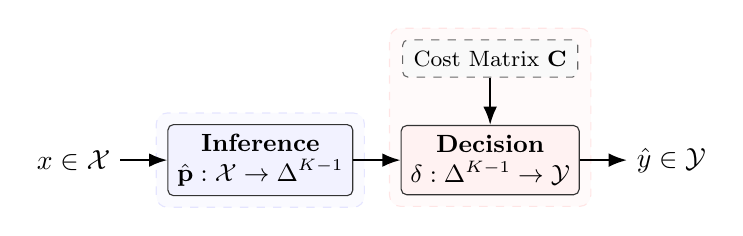
\begin{tikzpicture}[
        node distance=0.6cm,
        auto,
        block/.style={
            rectangle, 
            draw=black!80, 
            fill=blue!5, 
            align=center, 
            rounded corners=2pt, 
            minimum height=2.5em,
            minimum width=2.2cm,
            font=\small\bfseries
        },
        decision/.style={
            rectangle, 
            draw=black!80, 
            fill=red!5, 
            align=center, 
            rounded corners=2pt, 
            minimum height=2.5em,
            minimum width=2.2cm,
            font=\small\bfseries
        },
        param/.style={
            rectangle,
            draw=black!60,
            dashed,
            fill=gray!5,
            rounded corners=2pt,
            font=\footnotesize,
            inner sep=4pt
        },
        line/.style={
            draw, 
            -Latex, 
            thick
        }
    ]

        % --- Nodes ---
        
        \node (input) {$x \in \mathcal{X}$};

        \node [block, right=of input] (model) {\textbf{Inference} \\ $\hat{\mathbf{p}}: \mathcal{X} \to \Delta^{K-1}$};
        
        \node [decision, right=of model] (delta) {\textbf{Decision} \\ $\delta: \Delta^{K-1} \to \mathcal{Y}$};
        
        \node [right=of delta] (output) {$\hat{y} \in \mathcal{Y}$};
        
        \node [param, above=0.6cm of delta] (cost) {Cost Matrix $\mathbf{C}$};

        % --- Background Groups ---
        \begin{scope}[on background layer]
            \node [fit=(model), fill=blue!2, draw=blue!10, dashed, rounded corners, inner sep=4pt] {};
            \node [fit=(delta) (cost), fill=red!2, draw=red!10, dashed, rounded corners, inner sep=4pt] {};
        \end{scope}

        % --- Edges ---
        \path [line] (input) -- (model);
        \path [line] (model) -- (delta);
        \path [line] (delta) -- (output);
        \path [line] (cost) -- (delta);

    \end{tikzpicture}
\end{document} 
    \caption{The decomposition of the classification pipeline.}\label{fig:pipeline}
\end{figure}

\begin{enumerate}
    \item Inference Stage: An estimator $\hat{\mathbf{p}}: \mathcal{X} \to \Delta^{K-1}$ maps the input to the $(K-1)$-probability simplex, approximating the conditional distribution of $Y$ given $X$.
    \item Decision Stage: A decision rule $\delta: \Delta^{K-1} \to \mathcal{Y}$ maps the estimated probability vector to a discrete class label to satisfy a risk-minimization objective.
\end{enumerate}

The decomposition is sound when $\hat{\mathbf{p}}$ converges to the true conditional class probabilities. In finite-sample regimes or under model misspecification, $\hat{\mathbf{p}}$ deviates from $\boldsymbol{\eta}$ and the standard decision rules become suboptimal. The resulting excess risk (the gap between the decomposed classifier's risk and the Bayes Risk) is analyzed in Section~\ref{sec:excess_risk_miscalibration}.

\section{Inference: conditional probability estimation}\label{sec:inference}

Let $\Delta^{K-1} = \{ \mathbf{p} \in \mathbb{R}^K \mid \mathbf{p} \geq 0, \mathbf{1}^\top \mathbf{p} = 1 \}$ denote the standard $(K-1)$-simplex; throughout the dissertation, the unhatted symbol $\mathbf{p}$ stands for a generic element of $\Delta^{K-1}$ (e.g., the argument of a decision rule $\delta(\mathbf{p})$), distinct from the specific estimator output $\hat{\mathbf{p}}(x)$ introduced below. The \textit{conditional class probability} vector $\boldsymbol{\eta}: \mathcal{X} \to \Delta^{K-1}$ collects the per-class probabilities at $x$, with $k$-th entry
\begin{equation}
    \eta_k(x) := \mathbb{P}(Y=k \mid X=x), \quad k \in \mathcal{Y}.
\end{equation}
The inference stage uses the sample $\mathcal{S}$ to construct a measurable estimator $\hat{\mathbf{p}}: \mathcal{X} \to \Delta^{K-1}$ that approximates $\boldsymbol{\eta}$.

Since $\mathcal{S}$ contains only realized labels $y_i$ and not their generating probabilities $\boldsymbol{\eta}(x_i)$, $\hat{\mathbf{p}}$ is fit by minimizing a surrogate loss whose population minimizer recovers $\boldsymbol{\eta}$. The standard choices are the Logarithmic Loss (negative log-likelihood, equivalent to the Kullback-Leibler (KL) divergence between the empirical distribution and the model) and the Brier Score (squared error on the simplex); both belong to the family of \textit{strictly proper scoring rules}, whose population minimizer is $\boldsymbol{\eta}$ itself \citep{gneiting2007strictly}. If the hypothesis class $\mathcal{F}$ containing $\hat{\mathbf{p}}$ is sufficiently expressive ($\boldsymbol{\eta} \in \mathcal{F}$) and $N \to \infty$, optimizing these objectives guarantees that $\hat{\mathbf{p}}$ converges to $\boldsymbol{\eta}$ in probability.

\section{Decision: risk minimization}

Given the true conditional class probability vector $\boldsymbol{\eta}(x)$, the decision stage requires a mapping $\delta: \Delta^{K-1} \to \mathcal{Y}$ that selects a discrete action to minimize the expected loss. We define the \textit{Conditional Risk} $\mathcal{R}(\hat{y} \mid x)$ as the expected loss of taking a specific action $\hat{y} \in \mathcal{Y}$ with respect to the aleatoric uncertainty in $Y$,
\begin{equation}
    \mathcal{R}(\hat{y} \mid x) := \mathbb{E}_{Y \sim \boldsymbol{\eta}(x)} [C_{Y, \hat{y}}] = \sum_{k=0}^{K-1} C_{k, \hat{y}} \eta_k(x).
\end{equation}

In vectorized form, let $\mathbf{r}(x) \in \mathbb{R}_{\geq 0}^K$ denote the vector of conditional risks for all $K$ actions. Since the $i$-th column of $\mathbf{C}$ contains the costs of predicting class $i$,
\begin{equation}
    \mathbf{r}(x) = \left[ \mathcal{R}(0 \mid x), \dots, \mathcal{R}(K-1 \mid x) \right]^\top = \mathbf{C}^\top \boldsymbol{\eta}(x).
\end{equation}

The Bayes Optimal Decision Rule $h^*$ is the policy that selects the action minimizing this conditional risk
\begin{equation}\label{eq:bayes_optimal}
    h^*(x) = \underset{\hat{y} \in \mathcal{Y}}{\mathrm{argmin}} \,\, \mathcal{R}(\hat{y} \mid x),
\end{equation}
where ties are broken by selecting the smallest index. The corresponding Bayes Optimal Decision Rule on the simplex side of the decomposition $h = \delta \circ \hat{\mathbf{p}}$ is $\delta^*: \Delta^{K-1} \to \mathcal{Y}$,
\begin{equation}\label{eq:bayes_optimal_delta}
    \delta^*(\mathbf{p}) = \underset{\hat{y} \in \mathcal{Y}}{\mathrm{argmin}} \,\, [\mathbf{C}^\top \mathbf{p}]_{\hat{y}},
\end{equation}
so that $h^*(x) = \delta^*(\boldsymbol{\eta}(x))$. The following identity, which equates the Bayes Risk with the expectation of the pointwise minimum conditional risk, justifies treating $h^*$ as the optimal policy.

\begin{proposition}[Bayes risk identity]\label{prop:bayes_risk_identity}
For the Bayes Optimal Decision Rule $h^*$ defined in Eq.~(\ref{eq:bayes_optimal}),
\begin{equation}\label{eq:bayes_risk_identity}
    R(h^*) = \mathbb{E}_X \left[ \min_{\hat{y} \in \mathcal{Y}} \mathcal{R}(\hat{y} \mid X) \right] = \min_{h \in \mathcal{H}_{all}} \mathbb{E}_X \left[ \mathcal{R}(h(X) \mid X) \right] = R^*.
\end{equation}
\end{proposition}

\begin{proof}
Every $h \in \mathcal{H}_{all}$ satisfies the pointwise bound $\mathcal{R}(h(x) \mid x) \geq \min_{\hat{y}} \mathcal{R}(\hat{y} \mid x)$, and $h^*$ attains this minimum at every $x$, so monotonicity of the integral gives $R(h^*) = \mathbb{E}_X[\min_{\hat{y}} \mathcal{R}(\hat{y} \mid X)] = R^*$. The measurability of $h^*$ and finiteness of the integral are verified in Appendix~\ref{app:supplementary_proofs}.
\end{proof}

Geometrically, $\delta^*$ partitions the probability simplex $\Delta^{K-1}$ into the $K$ assigned regions $\{ \mathbf{p} \in \Delta^{K-1} \mid \delta^*(\mathbf{p}) = i \}$. Let $\mathbf{c}_i \in \mathbb{R}_{\geq 0}^K$ denote the $i$-th column of $\mathbf{C}$, i.e., the cost vector for predicting class $i$ across all possible true labels. Since the risk is linear in $\mathbf{p}$ ($\mathcal{R}(i \mid x) = \mathbf{c}_i^\top \boldsymbol{\eta}(x)$ when $\mathbf{p} = \boldsymbol{\eta}(x)$), the closed region $\mathcal{P}_i^*$ on which action $i$ minimizes the conditional risk is a convex polytope defined by the intersection of linear half-spaces
\begin{equation}
    \mathcal{P}_i^* = \{ \mathbf{p} \in \Delta^{K-1} \mid (\mathbf{c}_i - \mathbf{c}_j)^\top \mathbf{p} \leq 0, \forall j \neq i \}.
\end{equation}
The closed regions $\mathcal{P}_0^*, \dots, \mathcal{P}_{K-1}^*$ cover the simplex and overlap where conditional risks tie; the assigned region of action $i$ is $\mathcal{P}_i^*$ without the points at which a smaller index also minimizes the conditional risk, so the assigned regions form a partition but need not be closed. The boundaries between these regions are hyperplanes defined by the set of probability vectors where the conditional risks of two or more classes are equal. This geometric structure is analyzed in detail for the binary case in Section~\ref{sec:analytical_threshold} and for the multiclass case in Section~\ref{sec:geometry}.

\section{The plug-in principle}

Since $\boldsymbol{\eta}(x)$ is unknown in practice, we rely on the plug-in principle \citep{devroye1996probabilistic}, substituting the learned estimator $\hat{\mathbf{p}}(x)$ for the true conditional class probabilities. This yields the empirical decision rule $\hat{h}$,
\begin{equation}\label{argmin_risk}
    \hat{h}(x) = \underset{i \in \mathcal{Y}}{\mathrm{argmin}} \,\, [\mathbf{C}^\top \hat{\mathbf{p}}(x)]_i.
\end{equation}

The excess risk of the plug-in classifier can be bounded by the quality of the probability estimator.

\begin{proposition}[Bound on excess risk]\label{prop:excess_risk_bound}
Let $C_{max} = \max_{i,j} C_{ij}$ be the maximum entry in the cost matrix. The excess risk of the plug-in classifier $\hat{h}$ relative to the Bayes Optimal classifier $h^*$ is bounded by the $L_1$ estimation error
\begin{equation}
    R(\hat{h}) - R(h^*) \leq C_{max} \cdot \mathbb{E}_X \left[ \|\hat{\mathbf{p}}(X) - \boldsymbol{\eta}(X)\|_1 \right].
\end{equation}
\end{proposition}

\begin{proof}
Let $x$ be an arbitrary fixed input. Let $k^* = h^*(x)$ be the Bayes optimal action and $\hat{k} = \hat{h}(x)$ be the plug-in decision.
The conditional regret is defined as the difference in true conditional risk between the selected action and the optimal action,
\begin{equation}
    \Delta \mathcal{R}(x) = \mathcal{R}(\hat{k} \mid x) - \mathcal{R}(k^* \mid x) = \mathbf{c}_{\hat{k}}^\top \boldsymbol{\eta}(x) - \mathbf{c}_{k^*}^\top \boldsymbol{\eta}(x).
\end{equation}
We add and subtract the \textit{estimated} risks $\mathbf{c}_{\hat{k}}^\top \hat{\mathbf{p}}(x)$ and $\mathbf{c}_{k^*}^\top \hat{\mathbf{p}}(x)$ to the expression,
\begin{align}
    \Delta \mathcal{R}(x) &= \mathbf{c}_{\hat{k}}^\top \boldsymbol{\eta}(x) - \mathbf{c}_{\hat{k}}^\top \hat{\mathbf{p}}(x) + \underbrace{\left( \mathbf{c}_{\hat{k}}^\top \hat{\mathbf{p}}(x) - \mathbf{c}_{k^*}^\top \hat{\mathbf{p}}(x) \right)}_{\leq 0 \text{ by definition of } \hat{k}} + \mathbf{c}_{k^*}^\top \hat{\mathbf{p}}(x) - \mathbf{c}_{k^*}^\top \boldsymbol{\eta}(x) \\
    &\leq \mathbf{c}_{\hat{k}}^\top (\boldsymbol{\eta}(x) - \hat{\mathbf{p}}(x)) + \mathbf{c}_{k^*}^\top (\hat{\mathbf{p}}(x) - \boldsymbol{\eta}(x)) \\
    &= (\mathbf{c}_{\hat{k}} - \mathbf{c}_{k^*})^\top (\boldsymbol{\eta}(x) - \hat{\mathbf{p}}(x)).
\end{align}
Applying Hölder's inequality for the dot product ($\mathbf{a}^\top \mathbf{b} \leq \|\mathbf{a}\|_\infty \|\mathbf{b}\|_1$), we obtain
\begin{equation}
    \Delta \mathcal{R}(x) \leq \|\mathbf{c}_{\hat{k}} - \mathbf{c}_{k^*}\|_\infty \cdot \|\boldsymbol{\eta}(x) - \hat{\mathbf{p}}(x)\|_1.
\end{equation}
The term $\|\mathbf{c}_{\hat{k}} - \mathbf{c}_{k^*}\|_\infty$ represents the maximum absolute difference between the costs of action $\hat{k}$ and action $k^*$ for any ground truth class. Since $0 \leq C_{ij} \leq C_{max}$, this difference is bounded by $C_{max}$. Thus,
\begin{equation}
    \Delta \mathcal{R}(x) \leq C_{max} \|\boldsymbol{\eta}(x) - \hat{\mathbf{p}}(x)\|_1.
\end{equation}
Taking the expectation over $X$ yields the final result.
\end{proof}

The bound is linear in the $L_1$ estimation error with proportionality constant $C_{max}$, and both factors are worst-case. Pointwise, the conditional regret $\Delta\mathcal{R}(x)$ vanishes whenever $\hat{\mathbf{p}}(x)$ and $\boldsymbol{\eta}(x)$ lie in the same assigned region of $\delta^*$, that is, whenever the plug-in selects the Bayes-optimal action $\hat{h}(x) = h^*(x)$, so estimation error that does not cross a decision boundary contributes nothing to the excess risk, regardless of $C_{max}$. Sensitivity to estimation error is therefore concentrated near the boundaries between decision regions, where competing conditional risks are nearly equal and small perturbations of $\hat{\mathbf{p}}(x)$ can flip the argmin; the cost incurred when such a flip occurs is bounded by $\|\mathbf{c}_{\hat{k}} - \mathbf{c}_{k^*}\|_\infty \leq C_{max}$. When $C_{max} \gg 1$, even minor estimation errors that cross a boundary can produce substantial regret.

\section{Excess risk under probability miscalibration}\label{sec:excess_risk_miscalibration}

The excess risk incurred by the plug-in classifier relative to the Bayes optimal classifier is
\begin{equation}
    R(\hat{h}) - R(h^*) = \mathbb{E}_{X} \left[ \mathcal{R}(\hat{h}(X) \mid X) - \mathcal{R}(h^*(X) \mid X) \right].
\end{equation}

As established in Proposition~\ref{prop:excess_risk_bound}, this gap is bounded by the $L_1$ deviation of the estimator, but this worst-case bound obscures which features of the deviation actually drive the regret.

It is useful to distinguish failures of \textit{discrimination} from failures of \textit{calibration}. Modern classifiers (Deep Neural Networks, Gradient Boosted Machines) are often highly discriminative: they learn a monotonic transformation of the true conditional class probabilities, preserving the class ordering. But they frequently suffer from systematic calibration errors (shifts or scaling of probability values). When $\hat{\mathbf{p}}(x)$ is rank-preserving but miscalibrated, the analytical minimization in Eq.~(\ref{argmin_risk}) operates on a distorted probability landscape, and the boundaries between decision regions $\mathcal{P}_i^*$ shift to suboptimal positions. This suggests that the excess risk can be reduced by optimizing $\delta$ directly to compensate for the miscalibration of $\hat{\mathbf{p}}(x)$.

\section{The decision stage as a learning problem}\label{sec:decision_learning}

The decision stage can be seen as a supervised learning problem in its own right, nested inside the classification pipeline. Fix the estimator $\hat{\mathbf{p}}$, fitted on the sample $\mathcal{S}$, and let $\mathcal{V} = \{(x_i, y_i)\}_{i=1}^m$ be a held-out sample drawn i.i.d.\ from $\mathbb{P}$ and disjoint from $\mathcal{S}$. Writing $Z = \hat{\mathbf{p}}(X)$ for the induced representation on the simplex, the disjointness of $\mathcal{V}$ and $\mathcal{S}$ makes the pairs $(z_i, y_i) = (\hat{\mathbf{p}}(x_i), y_i)$ an i.i.d.\ sample from the joint law of $(Z, Y)$. The decision learner selects a rule $\delta$ from a hypothesis class $\mathcal{H}_{dec}$ of maps $\Delta^{K-1} \to \mathcal{Y}$ by minimizing the empirical risk
\begin{equation}\label{eq:decision_erm}
    \hat{R}(\delta) = \frac{1}{m} \sum_{i=1}^m C_{y_i, \delta(z_i)},
\end{equation}
whose population counterpart is the expected risk $R(\delta \circ \hat{\mathbf{p}}) = \mathbb{E}[C_{Y, \delta(Z)}]$ of Eq.~(\ref{eq:expected_risk}). Selecting $\delta$ by minimizing Eq.~(\ref{eq:decision_erm}) over $\mathcal{H}_{dec}$ is therefore empirical risk minimization (ERM), with input space $\Delta^{K-1}$, label space $\mathcal{Y}$, and the cost $C_{y, \hat{y}}$ as the loss. The name ``validation set'' is relative to the inference learner; for the decision learner, $\mathcal{V}$ is the training sample.

This viewpoint makes statistical learning theory applicable to the decision layer. When $\mathcal{V}$ is independent of the sample used to fit $\hat{\mathbf{p}}$, one may condition on the estimator and bound the generalization gap $R(\delta)-\hat{R}(\delta)$ in terms of the capacity of $\mathcal{H}_{dec}$ alone. This is the role of the capacity bounds below: the inference model may be highly complex and miscalibrated, but the learned decision rule can still generalize from a relatively small validation sample because it is chosen from a low-complexity class.

\subsection{Generalization guarantees for decision optimization}

The capacity of the decision-stage hypothesis class, or an integer upper bound on it, is denoted by $d_{dec}$. In the binary case, this capacity is measured by the VC dimension (Definition~\ref{def:vc_dimension}); in the multiclass setting, the corresponding capacity notion is introduced in the later multiclass chapters.

\begin{definition}[VC dimension]\label{def:vc_dimension}
    Let $\mathcal{H} \subseteq \{0,1\}^{\mathcal{X}}$.
    A set $S = \{x_1, \ldots, x_m\} \subset \mathcal{X}$ is shattered by $\mathcal{H}$
    if for every labeling $(b_1, \ldots, b_m) \in \{0,1\}^m$, there exists $h \in \mathcal{H}$
    with $h(x_i) = b_i$ for all $i$.
    The VC dimension $d_{VC}(\mathcal{H})$ is the cardinality of the largest
    shattered set.
\end{definition}

\begin{proposition}[Generalization bound for binary decision optimization]\label{prop:gen_bound}
Let $K = 2$ and $0 \leq C_{ij} \leq C_{max}$. Let $\mathcal{H}_{dec}$ be a class of binary decision rules with a countable subclass $\mathcal{H}_0$ of measurable rules that approximates every $\delta \in \mathcal{H}_{dec}$ pointwise: there is a sequence $(\delta_n)$ in $\mathcal{H}_0$ with $\delta_n(z) = \delta(z)$ for all sufficiently large $n$, at every input $z$. Let $d_{dec}$ be an integer with $d_{VC}(\mathcal{H}_{dec}) \leq d_{dec}$ and $1 \leq d_{dec} \leq m$, let $0 < \nu \leq 1$, and assume the validation sample $\mathcal{V}=\{(x_i,y_i)\}_{i=1}^m$ is drawn i.i.d.\ from $\mathbb{P}$ and independently of the sample used to fit $\hat{\mathbf{p}}$. With probability at least $1-\nu$ over the random draw of the validation sample, simultaneously for all $\delta \in \mathcal{H}_{dec}$, the true risk $R(\delta)$ is bounded by the empirical risk $\hat{R}(\delta)$ as
\begin{equation}\label{eq:generic_decision_gen_bound}
    R(\delta) \leq \hat{R}(\delta) + C_{max}\,\varepsilon(m,d_{dec},\nu),
\end{equation}
where one may take
\begin{equation}\label{eq:vc_decision_rate}
    \varepsilon(m,d_{dec},\nu)=2\sqrt{\frac{d_{dec}\log\frac{2em}{d_{dec}}+\log\frac{4}{\nu}}{m}}.
\end{equation}
\end{proposition}

\begin{proof}
Condition on the fitted estimator $\hat{\mathbf{p}}$, which is fixed with respect to the independent validation sample. Write $Z=\hat{\mathbf{p}}(X)$ and $z_i=\hat{\mathbf{p}}(x_i)$. The decision learner is then an ordinary empirical-risk-minimization problem over the validation pairs $(z_i,y_i)$, with loss
\begin{equation}\label{eq:decision_loss}
    \ell_\delta(z,y)=C_{y,\delta(z)}.
\end{equation}
This loss is not the $0/1$ loss of a binary classifier, so we decompose it into level sets. List its distinct positive values as $0 < v_1 < \cdots < v_q \leq C_{max}$, with $q \leq 4$, and set $v_0 = 0$; if there is no positive value the conclusion is immediate. Then
\begin{equation*}
    \ell_\delta(z,y)=\sum_{a=1}^{q}(v_a-v_{a-1})\,\mathbb{I}\{\ell_\delta(z,y)\geq v_a\}.
\end{equation*}
For each fixed level $v_a$, the binary class $(z,y)\mapsto\mathbb{I}\{C_{y,\delta(z)}\geq v_a\}$, $\delta \in \mathcal{H}_{dec}$, has VC dimension at most $d_{dec}$: a shattered sample cannot repeat an input $z$, because each such input has only two possible predictions, so at every sample point the level indicator must take different values for the two predictions, and the rules of $\mathcal{H}_{dec}$ must therefore realize every binary labeling of the distinct inputs.

Restrict first to $\mathcal{H}_0$. Apply the VC uniform-convergence bound of \citet[Corollary~3.19]{mohri2018foundations} to each level, with failure probability $\nu/4$, viewing the indicator as the $0/1$ loss of a classifier on examples relabelled with the constant label $0$. A union bound over the at most four levels gives, simultaneously for every level and every rule of $\mathcal{H}_0$, a population-minus-empirical gap at most
\begin{equation*}
    \sqrt{\frac{2d_{dec}\log(em/d_{dec})}{m}}+\sqrt{\frac{\log(4/\nu)}{2m}}.
\end{equation*}
The coefficients $v_a - v_{a-1}$ are nonnegative and sum to at most $C_{max}$, so multiplying and summing gives the same gap times $C_{max}$. Finally, $\sqrt{a}+\sqrt{b}\leq\sqrt{2(a+b)}$ and $\log(em/d_{dec})\leq\log(2em/d_{dec})$ bound this expression by Eq.~(\ref{eq:vc_decision_rate}). On the same event the bound extends to every $\delta\in\mathcal{H}_{dec}$: along its approximating sequence, bounded costs and eventual pointwise agreement give convergence of the population risks by dominated convergence, and the empirical risks on the fixed sample are eventually equal to that of $\delta$. Passing to the limit gives Eq.~(\ref{eq:generic_decision_gen_bound}).
\end{proof}

We will use a clean form of this guarantee in the chapters that follow. Under the hypotheses of Proposition~\ref{prop:gen_bound} without the restriction $d_{dec} \leq m$, with probability at least $1-\nu$, simultaneously for all $\delta \in \mathcal{H}_{dec}$,
\begin{equation}\label{eq:clean_gen_bound}
    R(\delta) \leq \hat{R}(\delta) + c_{bin}(m,\nu)\, C_{max} \sqrt{\frac{d_{dec}}{m}},
\end{equation}
where
\begin{equation*}
    c_{bin}(m,\nu)=\sqrt{2\log(em)}+\sqrt{\frac{\log(4/\nu)}{2}}.
\end{equation*}
For $m \geq d_{dec}$ this follows from the two-term gap in the proof, since $d_{dec} \geq 1$; for $m < d_{dec}$ the additive term exceeds $C_{max}$ and the bound is immediate. The factor $c_{bin}$ depends on $m$ and $1/\nu$ through logarithms, so the sufficient condition $m \geq c_{bin}(m,\nu)^2 C_{max}^2\, d_{dec}/\epsilon^2$ for a gap at most $\epsilon$ retains that dependence. In the multiclass case $d_{dec}$ is given by the multiclass capacity measure introduced later.

\subsection{Hypothesis-class complexity of decision rules}

The bound in Proposition~\ref{prop:gen_bound} is useful precisely because the decision-stage classes considered in this dissertation have low capacity. While the estimator $\hat{\mathbf{p}}$ may belong to a high-complexity class, the decision optimization occurs in a much smaller space.

In the binary regime ($K=2$), the decision rule acts on a scalar probability estimate $z \in [0, 1]$. The standard decision rule is a threshold function $\delta_\tau(z) = \mathbb{I}(z \geq \tau)$ (Lemma~\ref{lem:threshold_optimality} shows this form is Bayes-optimal under reasonable cost conditions).

\begin{lemma}\label{lem:vc_thresh}
Let $\mathcal{H}_{thresh} = \{ \delta_\tau : [0,1] \to \{0,1\} \mid \tau \in [0,1] \}$ be the class of threshold indicator functions $\delta_\tau(z) = \mathbb{I}(z \geq \tau)$. The VC dimension of this class is $d_{VC}(\mathcal{H}_{thresh}) = 1$.
\end{lemma}

\begin{proof}
The class shatters a single point, since varying $\tau$ around it realizes both labels, but no set of two points $z_1 < z_2$, since $\delta_\tau$ cannot label the smaller point positive and the larger negative ($z_1 \geq \tau > z_2$ contradicts $z_1 < z_2$). Hence $d_{VC}(\mathcal{H}_{thresh}) = 1$. Appendix~\ref{app:supplementary_proofs} gives the full argument.
\end{proof}

The threshold class satisfies the approximation hypothesis of Proposition~\ref{prop:gen_bound}. For each $\tau \in [0,1]$, rational thresholds in $[0,1]$ approaching $\tau$ from below, or the constant sequence $0$ when $\tau = 0$, give decisions that agree with $\delta_\tau$ eventually at every $z$, including $z = \tau$.

In the multiclass setting ($K>2$), the decision rule partitions $\Delta^{K-1}$ into $K$ regions, and the relevant combinatorial complexity depends on the chosen parameterization of $\delta$. Subsequent chapters introduce the specific multiclass partition families and bound their capacity using the appropriate multiclass notions; the resulting bounds are at most quadratic in $K$.

These capacity bounds explain why decision optimization can be statistically feasible: the decision layer is much smaller than the inference model, and its sample complexity scales with $d_{dec}$ rather than with the complexity of $\hat{\mathbf{p}}$. However, low capacity does not guarantee that the empirically selected rule improves on the analytical plug-in rule. Even in the binary case, where the decision class consists only of thresholds and has VC dimension one, choosing the threshold by minimizing validation risk can overfit finite-sample fluctuations. This is especially problematic when many thresholds have nearly indistinguishable true risk, so that the empirical minimizer is selected by noise rather than by a meaningful improvement in expected cost. In such regimes, the learned threshold may perform worse than the default plug-in rule, motivating the use of cross-validation or other model-selection safeguards in the empirical chapters.
%!TeX root=../carlo_master.tex
\chapter{Binary classification ($K=2$)}\label{sec:binary}

This chapter specializes the framework of Chapter~\ref{sec:theory} to $K=2$: we derive the classical Elkan threshold \citep{elkan2001foundations}, analyze its fragility under probability miscalibration, and develop empirical threshold optimization as an alternative.

\section{Problem setup and notation}

Let $\mathcal{Y} = \{0, 1\}$, with class $0$ as ``Negative'' and class $1$ as ``Positive''. Following the decomposition $h(x) = \delta(\hat{\mathbf{p}}(x))$, the inference stage learns $\hat{\mathbf{p}}: \mathcal{X} \to \Delta^1$.

Since $\eta_0(x) + \eta_1(x) = 1$, the estimator output can be reduced to a scalar. We write $\eta(x) := \eta_1(x) = \mathbb{P}(Y{=}1 \mid X{=}x)$ for the true conditional class probability, and $\hat{p}(x) := \hat{p}_1(x)$ for its estimate.

The decision rule $\delta: [0, 1] \to \{0, 1\}$ converts this score into a discrete action. We parameterize it by a threshold $\tau \in [0, 1]$,
\begin{equation}\label{eq:threshold_rule}
    \delta_\tau(\hat{p}(x)) = \mathbb{I}(\hat{p}(x) \geq \tau) = \begin{cases}
        1 & \text{if } \hat{p}(x) \geq \tau \\
        0 & \text{if } \hat{p}(x) < \tau
    \end{cases}.
\end{equation}
Optimizing $\delta$ thus reduces to finding the threshold $\tau^*$ that minimizes the expected risk for the fixed estimator $\hat{p}$.

\section{Analytical threshold derivation}\label{sec:analytical_threshold}

The $2 \times 2$ Cost Matrix $\mathbf{C}$ has entry $C_{ij}$ for the penalty of predicting class $j$ when the true class is $i$, covering True Negatives ($C_{00}$), False Positives ($C_{01}$), False Negatives ($C_{10}$), and True Positives ($C_{11}$).

\begin{table}[H]
    \centering
    \begin{tabular}{c|cc}
         & Predict Negative (0) & Predict Positive (1) \\
         \hline
         Actual Negative (0) & $C_{00}$ & $C_{01}$ \\
         Actual Positive (1) & $C_{10}$ & $C_{11}$
    \end{tabular}
    \caption{The Binary Cost Matrix.}
\end{table}

Following \citet{elkan2001foundations}, we impose \textit{reasonableness conditions}: misclassification must cost strictly more than a correct decision,
\begin{equation}\label{eq:reasonableness}
    C_{01} > C_{00} \quad \text{and} \quad C_{10} > C_{11}.
\end{equation}
If exactly one of these conditions is violated, one action weakly dominates the other and the optimal policy degenerates to a constant rule that ignores $x$ entirely. If both are violated, the problem is equivalent under label swap to a standard one with reasonable costs.

We first show that under these conditions, the risk-minimizing policy is always a threshold function, justifying the parameterization $\delta_\tau$ introduced in Eq.~\ref{eq:threshold_rule}.

\begin{lemma}[Optimality of threshold policies]\label{lem:threshold_optimality}
If the cost matrix satisfies the reasonableness conditions (Eq.~\ref{eq:reasonableness}), the Bayes Optimal decision rule $h^*(x)$ is equivalent to a threshold function $\delta_\tau(\eta(x)) = \mathbb{I}(\eta(x) \geq \tau)$ for a unique scalar $\tau \in [0, 1]$.
\end{lemma}

\begin{proof}
The risk-minimizing rule predicts class 1 whenever the conditional risk of predicting 1 is at most that of predicting 0, equivalently whenever the differential risk function $g(\eta) = \mathcal{R}(0 \mid \eta) - \mathcal{R}(1 \mid \eta)$ is non-negative; at $g(\eta) = 0$ the two conditional risks are equal, so either action attains the pointwise minimum and the choice between them does not affect the risk. Expanding the risks,
\begin{align}
    g(\eta) &= [C_{00}(1-\eta) + C_{10}\eta] - [C_{01}(1-\eta) + C_{11}\eta] \\
    &= \eta(C_{10} - C_{00} + C_{01} - C_{11}) + (C_{00} - C_{01}) \\
    &= \eta \underbrace{\left[ (C_{10} - C_{11}) + (C_{01} - C_{00}) \right]}_{m} - \underbrace{(C_{01} - C_{00})}_{c}.
\end{align}
This yields a linear function $g(\eta) = m\eta - c$. The reasonableness conditions imply that both term groups in $m$ are strictly positive: $(C_{10} - C_{11}) > 0$ and $(C_{01} - C_{00}) > 0$, so $m > 0$. Similarly, $c = C_{01} - C_{00} > 0$. Since $g(\eta)$ is strictly monotonically increasing with respect to $\eta$, it crosses zero exactly once at the unique root $\tau = c/m$.

It remains to verify that $\tau \in (0, 1)$. Since $c > 0$ and $m > 0$, we have $\tau > 0$. Moreover, $m = c + (C_{10} - C_{11})$ with $(C_{10} - C_{11}) > 0$, so $m > c$, which gives $\tau = c/m < 1$. Thus $\tau \in (0, 1)$ and $g(\eta) \geq 0$ if, and only if, $\eta \geq \tau$. Hence $\mathbb{I}(\eta \geq \tau)$ attains the minimum conditional risk at every $\eta$ and is Bayes-optimal; it may differ from the smallest-index selection of Eq.~(\ref{eq:bayes_optimal}) only on the tie set $\{\eta = \tau\}$, where both actions are risk-minimizers, so both rules attain the Bayes risk $R^*$.
\end{proof}

The Theoretical Optimal Threshold $p^*$ is the decision boundary where risks are equal ($g(\eta)=0$),
\begin{equation}\label{eq:elkan_threshold}
    p^* = \frac{C_{01} - C_{00}}{(C_{01} - C_{00}) + (C_{10} - C_{11})}.
\end{equation}

Under symmetric costs (0/1 loss, $C_{01}=C_{10}=C$, diagonal zero, with $C=1$ without loss of generality), this reduces to $p^* = 0.5$. The familiar $p > 0.5$ threshold, which many machine learning frameworks use by default, is thus an implicit assumption of symmetric loss.

Under asymmetric costs, the threshold must shift. For example, if a false negative costs ten times more than a false positive ($C_{10}=10, C_{01}=1$), the threshold drops to $p^* \approx 0.09$: the agent must act on weak signals to avoid missing positive instances.

The analytical threshold (Eq.~\ref{eq:elkan_threshold}) is optimal when $\hat{p}(x) = \eta(x)$ almost everywhere. In practice, this does not reliably hold. Modern classifiers are often highly discriminative (preserving the ordinal ranking of the true conditional class probabilities) but systematically miscalibrated: Deep Neural Networks tend toward overconfidence \citep{guo2017calibration}, pushing probability mass toward 0 and 1, while regularized models may exhibit oversmoothing, contracting predictions toward the marginal prior even with decent discriminative performance. When the analytical rule is applied to miscalibrated scores, the realized decision boundary diverges from the intended risk profile. Two complementary strategies address this: \textit{post-hoc calibration}, which corrects the probability estimates before thresholding, and \textit{empirical threshold optimization}, which bypasses the calibration problem entirely by selecting the threshold that directly minimizes empirical risk.

\section{Post-hoc probability calibration}\label{sec:calibration}

The core issue of the plug-in rule is that $\hat{p}(x)$ does not faithfully represent $\eta(x)$. A natural fix is to \textit{recalibrate} the estimator's outputs before applying the analytical rule. We formalize calibration, present the standard diagnostic, and describe four post-hoc methods evaluated in our experiments.

\subsection{Defining and measuring calibration}

\begin{definition}[Perfect calibration]\label{def:calibration}
An estimator $\hat{p} \colon \mathcal{X} \to [0,1]$ is perfectly calibrated with respect to $\mathbb{P}$ if
\begin{equation}\label{eq:perfect_calibration}
    \mathbb{P}(Y = 1 \mid \hat{p}(X) = q) = q, \quad \text{for } \mathbb{P}_{\hat{p}(X)}\text{-almost every } q \in [0,1].
\end{equation}
\end{definition}

Perfect calibration means that among all instances assigned predicted probability $q$, the true conditional proportion of positives equals $q$ exactly. This is a \textit{marginal} property: it constrains the distribution of $Y$ given the \textit{scalar output} $\hat{p}(X)$, not the full input $X$. It is strictly weaker than pointwise consistency ($\hat{p}(x) = \eta(x)$ almost everywhere) and independent of discriminative power: the trivial estimator $\hat{p}(x) = \bar{y}$ (marginal class frequency) is perfectly calibrated yet carries no information about individual instances \citep{degroot1983comparison}.

The standard finite-sample diagnostic is the Expected Calibration Error (ECE). Given $B$ bins $\{I_b\}_{b=1}^B$ partitioning $[0,1]$,
\begin{equation}\label{eq:ece}
    \widehat{\mathrm{ECE}} = \sum_{b=1}^{B} \frac{|I_b|}{n} \left| \bar{y}_b - \bar{p}_b \right|,
\end{equation}
where $\bar{y}_b$ and $\bar{p}_b$ denote the average true label and average predicted probability within bin $I_b$, respectively \citep{naeini2015obtaining}.

\subsection{Post-hoc calibration methods}

Post-hoc methods fit a transformation $g: [0,1] \to [0,1]$ on held-out data so that $g(\hat{p}(x))$ is better calibrated than $\hat{p}(x)$. The base estimator is \textit{frozen}: these methods remap outputs without retraining. We describe the four methods used in our experiments, ordered by increasing expressiveness.

\paragraph{Temperature scaling.} The simplest parametric method rescales the logit by a single scalar $T > 0$ \citep{guo2017calibration},
\begin{equation}\label{eq:temperature_scaling}
    g_T(\hat{p}) = \sigma\!\left(\frac{z(\hat{p})}{T}\right), \quad z(\hat{p}) = \log \frac{\hat{p}}{1 - \hat{p}},
\end{equation}
where $\sigma$ denotes the logistic sigmoid. When $T > 1$, the transformation softens overconfident predictions toward $0.5$; when $T < 1$, it sharpens underconfident ones. The parameter $T$ is fitted by minimizing the negative log-likelihood on held-out data, and the transformation preserves the ranking of instances.

\paragraph{Platt scaling.} This method fits a two-parameter sigmoid on the classifier's raw score $s(x)$ \citep{platt1999probabilistic,niculescuMizil2005predicting},
\begin{equation}\label{eq:platt_scaling}
    g_{a,b}(s) = \sigma\!\left(a \cdot s + b\right),
\end{equation}
with $(a, b) \in \mathbb{R}^2$ fitted by minimizing the negative log-likelihood. The slope $a$ corrects miscalibrated confidence spread (analogous to temperature) and the intercept $b$ a systematic score bias. Platt scaling can correct any monotonic sigmoid distortion of $s(x)$ but cannot model non-monotonic miscalibration.

\paragraph{Isotonic regression.} A non-parametric method that fits a monotone non-decreasing step function $m: [0,1] \to [0,1]$ \citep{zadrozny2002transforming}. On a calibration set, examples are first sorted by their predicted scores,
$\hat p(x_{(1)}) \le \cdots \le \hat p(x_{(n)})$, and the method solves the finite-dimensional constrained least-squares problem
\begin{equation}\label{eq:isotonic}
    z^* = \underset{0 \le z_1 \le \cdots \le z_n \le 1}{\mathrm{argmin}}
    \sum_{i=1}^{n} (z_i - y_{(i)})^2,
\end{equation}
where $z_i = m(\hat p(x_{(i)}))$ is the calibrated value assigned to the $i$-th sorted score. The solution is obtained efficiently by pooling adjacent blocks whose empirical label averages violate monotonicity, yielding a monotone step function $m^*$. Because $m^*$ is unconstrained in functional form beyond monotonicity, isotonic regression can correct \textit{any} monotonic distortion, not just sigmoid ones, making it strictly more expressive than Platt scaling.

\paragraph{Dirichlet calibration.} The most expressive parametric method in our suite learns an affine transformation in log-probability space \citep{kull2019beyond},
\begin{equation}\label{eq:dirichlet_calibration}
    g_{\mathbf{W}, \mathbf{b}}(\hat{\mathbf{p}}) = \mathrm{softmax}\!\left(\mathbf{W} \log \hat{\mathbf{p}} + \mathbf{b}\right),
\end{equation}
where $\mathbf{W} \in \mathbb{R}^{K \times K}$ and $\mathbf{b} \in \mathbb{R}^K$. In the binary case ($K=2$), this reduces to three effective parameters after accounting for the softmax normalization, since $z_1 - z_0 = a \cdot \log\hat p - a \cdot \log(1-\hat p) + (b_1 - b_0)$ when $\mathbf{W} = a \mathbf{I}$. Logit-space Platt scaling, $\sigma(a \cdot z(\hat p) + b)$, is therefore recovered when $\mathbf{W}$ is a scalar multiple of the identity (with $b = b_1 - b_0$), and temperature scaling is the further restriction $b_0 = b_1$. The parameters are fitted by minimizing the negative log-likelihood.

\subsection{The calibrate-then-decide framework}

The calibration methods above can be composed with the analytical threshold to form a two-stage decision pipeline: (1)~fit a calibrator $g$ on held-out data, then (2)~apply the cost-derived threshold $p^*$ from Equation~(\ref{eq:elkan_threshold}) to the recalibrated scores $g(\hat{p}(x))$.

\begin{proposition}[Optimality of calibrate-then-decide]\label{prop:calibrate_then_decide}
Assume the reasonableness conditions (Eq.~\ref{eq:reasonableness}), let $g: [0,1] \to [0,1]$ be a measurable post-hoc calibrator, and define the composite decision rule $\delta_g(x) = \mathbb{I}(g(\hat{p}(x)) \geq p^*)$. If $g(\hat{p}(x)) = \eta(x)$ for $\mathbb{P}_X$-almost every $x$, a condition that implies perfect calibration, then $\delta_g$ attains the Bayes risk, $R(\delta_g) = R^*$, and agrees with the Bayes-optimal decision rule $h^*$ (Eq.~\ref{eq:bayes_optimal}) almost everywhere off the tie set $\{x : \eta(x) = p^*\}$.
\end{proposition}
\begin{proof}
Immediate from the premise, which gives $\delta_g(x) = \mathbb{I}(\eta(x) \geq p^*)$ almost everywhere, and Lemma~\ref{lem:threshold_optimality}; on the tie set both actions minimize the conditional risk, although $\delta_g$ selects $1$ and $h^*$ selects $0$. See Appendix~\ref{app:supplementary_proofs}.
\end{proof}

In practice, perfect calibration is unattainable: the residual error after post-hoc correction, combined with the calibrator's own finite-sample variance, leaves the analytical threshold on recalibrated scores an approximation. The next subsection bypasses calibration entirely and optimizes the threshold against the operational objective.

\section{Empirical threshold optimization}

An alternative is empirical threshold optimization, following foundational work on cost-sensitive thresholding \citep{sheng2006thresholding} and widely used in applied machine learning. Rather than deriving the decision boundary from the cost matrix and probability estimates, which may be flawed, $\tau$ becomes a learnable parameter of $\delta_\tau$, optimized directly against the operational objective on real data.

Let $\mathcal{V} = \{(x_i, y_i)\}_{i=1}^m$ be a held-out validation set drawn i.i.d.\ from $\mathbb{P}$. We define the empirical risk objective $\hat{R}(\tau)$ for a candidate threshold $\tau$ as the average realized cost over the sample,
\begin{equation}\label{eq:empirical_risk_obj}
    \hat{R}(\tau) = \frac{1}{m} \sum_{i=1}^m \left[ \mathbb{I}(\hat{p}(x_i) \ge \tau) C_{y_i, 1} + \mathbb{I}(\hat{p}(x_i) < \tau) C_{y_i, 0} \right],
\end{equation}
where $C_{y_i, k}$ denotes the cost of predicting class $k$ given the true label $y_i$. The optimal empirical threshold is the scalar that minimizes this discontinuous, piecewise-constant objective,
\begin{equation}
    \tau_{emp} = \underset{\tau \in [0, 1]}{\mathrm{argmin}} \,\, \hat{R}(\tau).
\end{equation}

\subsection{Threshold grid search}\label{sec:threshold_grid_search}

Since $\hat{R}(\tau)$ is piecewise-constant with jumps only at the distinct predicted scores, only finitely many candidate thresholds need to be evaluated \citep{provost2001robust}. In practice we approximate this by evaluating $\hat{R}$ over a uniform grid of $G$ thresholds,
\begin{equation}
    \mathcal{T} = \left\{ \frac{g}{G-1} \;\middle|\; g \in \{0, \dots, G-1\} \right\} \subset [0,1],
\end{equation}
and returning
\begin{equation}
    \hat{\tau} = \underset{\tau \in \mathcal{T}}{\mathrm{argmin}} \; \hat{R}(\tau).
\end{equation}
For each candidate $\tau_k \in \mathcal{T}$, the confusion counts are computed simultaneously for all $k$ via broadcasting, so evaluating all $G$ candidates costs $G\,m$ confusion-count updates and is vectorization-friendly.


\subsection{Cross-validated threshold optimization}\label{sec:cv_threshold}

To avoid dedicating a fixed portion of the training data to the decision stage, the threshold can be optimized via $F$-fold cross-validation (CV), treating $\tau$ as a hyperparameter. The training data $\mathcal{D}_{train}$ are partitioned into $F$ disjoint folds $\mathcal{D}_1, \dots, \mathcal{D}_F$, and a grid $\mathcal{T} \subset [0, 1]$ of candidate thresholds is fixed.

For each fold $k$, the estimator $\hat{p}_{-k}$ is trained on $\mathcal{D}_{train} \setminus \mathcal{D}_k$ and its predicted probabilities on $\mathcal{D}_k$ are used to evaluate the per-fold empirical risk $\hat{R}_k(\tau)$. Averaging across folds yields the cross-validated risk
\[ \hat{R}_{CV}(\tau) = \frac{1}{F} \sum_{k=1}^F \hat{R}_k(\tau), \]
and the selected threshold minimizes this average,
\[ \tau_{emp} = \underset{\tau \in \mathcal{T}}{\mathrm{argmin}} \,\, \hat{R}_{CV}(\tau). \]
Averaging across splits reduces sensitivity to any single held-out fold. Once $\tau_{emp}$ is determined, the final estimator $\hat{p}$ is retrained on all of $\mathcal{D}_{train}$. A cross-validated threshold tuner of this kind is available in scikit-learn as \texttt{TunedThresholdClassifierCV} (added in version 1.5) \citep{pedregosa2011scikit}, which selects the decision threshold of a binary classifier against a user-supplied scoring function, with $5$-fold stratified cross-validation by default.

\section{Capacity of the binary decision and calibration classes}\label{sec:binary_sample_complexity}

Both the empirical threshold and the post-hoc calibrators are fitted on a finite validation set, so their hypothesis-class capacity controls the generalization gap of that fit. This section collects the binary capacity statements, which the experiments of Chapter~\ref{sec:binary_experiments} draw on.

\subsection{Generalization bound for the empirical threshold}

Empirical threshold optimization is the binary instance of the decision-stage learning problem of Section~\ref{sec:decision_learning}: $\mathcal{V}$ is its training sample, $\mathcal{H}_{thresh}$ its hypothesis class, and $\tau_{emp}$ its empirical risk minimizer, so the bound below is its generalization guarantee.

Since the VC dimension of threshold functions is $d_{VC}=1$ (Lemma~\ref{lem:vc_thresh}), the clean form~\eqref{eq:clean_gen_bound} of Proposition~\ref{prop:gen_bound} gives
\begin{equation}
    R(\tau_{emp}) \leq \hat{R}(\tau_{emp}) + c\, C_{max} \sqrt{\frac{1}{m}},
\end{equation}
with probability at least $1-\nu$, where $c = c_{bin}(m,\nu)$ is the logarithmic factor of~\eqref{eq:clean_gen_bound}; the bound holds simultaneously over all thresholds, and in particular for the data-dependent $\tau_{emp}$. Provided $m$ is large enough relative to $C_{max}$, the empirical optimization converges to the optimal operating point for the fixed estimator $\hat{p}$, effectively re-calibrating the decision boundary to account for estimation errors. The proviso is binding in practice: on a small dedicated validation split the $\sqrt{1/m}$ term need not be negligible, and the empirical threshold can fail to improve on the analytical plug-in. The low VC dimension is therefore necessary but not sufficient; the binding constraint is the label budget of the held-out partition, which the cross-validated variant enlarges.

\subsection{Calibrator complexity}

Since calibrators are real-valued functions ($g: [0,1] \to [0,1]$), the relevant complexity measure is the \textit{pseudo-dimension} \citep{pollard1984convergence,haussler1992decision}, a generalization of VC dimension to real-valued function classes.

\begin{definition}[Pseudo-dimension]\label{def:pseudo_dimension}
    Following \citet[Definition~11.2]{anthony1999neural}, let $\mathcal{G} \subseteq \mathbb{R}^{\mathcal{X}}$ be a class of real-valued functions on $\mathcal{X}$. A set of points $\{x_1, \ldots, x_m\} \subset \mathcal{X}$ is pseudo-shattered by $\mathcal{G}$ if there exist witnesses $r_1, \ldots, r_m \in \mathbb{R}$ such that for every binary labeling $(b_1, \ldots, b_m) \in \{0,1\}^m$, there exists $g \in \mathcal{G}$ satisfying
    \begin{equation}
        g(x_i) \geq r_i \iff b_i = 1, \quad \text{for all } i = 1, \ldots, m.
    \end{equation}
    The pseudo-dimension $d_P(\mathcal{G})$ is the cardinality of the largest set that can be pseudo-shattered by $\mathcal{G}$.
\end{definition}

When $\mathcal{G}$ is binary-valued, pseudo-dimension coincides with VC dimension, and a validation set of size proportional to $d_P/\epsilon^2$ (that is, $m \geq c\, d_P/\epsilon^2$) controls the empirical loss \citep[Chapter~11]{anthony1999neural}.

\begin{proposition}[Pseudo-dimension of binary calibrators]\label{prop:calibrator_complexity}
Let $\mathcal{H}_{temp}$, $\mathcal{H}_{platt}$, and $\mathcal{H}_{dir}$ denote the temperature, Platt, and binary Dirichlet calibrator families defined in Eqs.~\eqref{eq:temperature_scaling},~\eqref{eq:platt_scaling}, and~\eqref{eq:dirichlet_calibration}, with $W = 1$, $2$, and $3$ free parameters respectively. Each is a fixed strictly increasing transform (the sigmoid, or the softmax in the binary reduction) of a score that is affine in its $W$ parameters; pseudo-dimension is invariant under such a transform and is at most the dimension of the affine score family, so by \citet[Theorem~11.4]{anthony1999neural}, $d_P(\mathcal{H}_{temp}) \leq 1$, $d_P(\mathcal{H}_{platt}) \leq 2$, and $d_P(\mathcal{H}_{dir}) \leq 3$.
\end{proposition}

Isotonic regression over $\mathcal{M}_\uparrow$ is non-parametric and has unbounded pseudo-dimension, so its complexity is not captured by the framework above; control results in other measures are available in the literature \citep{meyer2000degrees, zhang2002risk}.

%!TeX root=../carlo_master.tex
\chapter{Experimental analysis: binary classification}\label{sec:binary_experiments}

This chapter evaluates the decision strategies of Chapter~\ref{sec:binary} on fourteen datasets, ten base classifiers, and ten objectives (five cost matrices and five non-decomposable maximization metrics; see Section~\ref{sec:binary_objectives}). The cost-blind plug-in rule is suboptimal in nearly every regime considered, and two routes recover competitive performance: post-hoc calibration composed with the analytical Elkan threshold, and cross-validated empirical optimization of the threshold (EmpiricalCV). EmpiricalCV wins or ties the per-row best strategy on $87\%$ of cost cells and $99.9\%$ of maximization-metric cells. Post-hoc calibration composed with the analytical rule is the highest-rate strategy among the non-tuning options on miscalibrated non-neural estimators under decomposable cost objectives.

\section{Experimental setup}

We use a standardized protocol that holds the data partition, preprocessing, and base estimator fixed across decision strategies for a given dataset.

\subsection{Datasets}
The benchmark draws fourteen binary datasets from OpenML \citep{vanschoren2014openml}, selected along four axes. First, size spread: the three sample-size tiers (small with $N < 10^3$; medium, $10^3 \leq N < 10^4$; large, $N \geq 10^4$) vary the budget available to the strategies that consume a held-out partition (calibrator fits and the empirical threshold search), so the comparison is exercised from tens of positives in the validation split up to tens of thousands. Second, imbalance diversity: prevalence ratios span $1.0$ (\textit{madelon}) to $42.0$ (\textit{mammography}), with coverage at every order of magnitude in between, so the cost-asymmetric objectives can be exercised under both near-balanced and high-skew regimes. Third, overlap with prior cost-sensitive learning benchmarks: \textit{sonar}, \textit{pima\_diabetes}, and \textit{german\_credit} appear in \citet{sheng2006thresholding}, and \textit{adult} is used in \citet{elkan2001foundations}, so part of the pool is directly comparable to earlier results. Fourth, task difficulty: the pool spans easy problems on which the base classifiers reach near-ceiling discrimination and harder ones on which every estimator in the benchmark remains well below ceiling, so the decision strategies are evaluated on top of probability estimates of widely varying quality. Table~\ref{tab:dataset-summary-binary} lists the per-dataset sample sizes, feature counts, and class prevalences.

\begin{table}[H]
  \centering
  \caption{Summary of binary classification datasets used in the experiments. Superscripts denote OpenML dataset IDs. Numerical and Categorical are the counts of raw numerical and categorical input features; Encoded is the model input dimensionality after one-hot encoding of the categorical features. The imbalance ratio (IR) is the size of the majority class divided by that of the minority class.}%
  \label{tab:dataset-summary-binary}
  \resizebox{\textwidth}{!}{%
  \begin{tabular}{lrrrrl}
\toprule
 &  & \multicolumn{3}{c}{Features} &  \\
\cmidrule(lr){3-5}
Dataset & Samples & Numerical & Categorical & Encoded & IR \\
\midrule
sonar\textsuperscript{\tiny 40}~\citep{gorman1988sonar} & 208 & 60 & 0 & 60 & 1.1 \\
ionosphere\textsuperscript{\tiny 59}~\citep{sigillito1989ionosphere} & 351 & 34 & 0 & 34 & 1.8 \\
wdbc\textsuperscript{\tiny 1510}~\citep{street1993wdbc} & 569 & 30 & 0 & 30 & 1.7 \\
pima\_diabetes\textsuperscript{\tiny 37}~\citep{smith1988diabetes} & 768 & 8 & 0 & 8 & 1.9 \\
german\_credit\textsuperscript{\tiny 31}~\citep{hofmann1994germancredit} & 1000 & 7 & 13 & 61 & 2.3 \\
pc3\textsuperscript{\tiny 1050}~\citep{sayyadshirabad2005promise} & 1563 & 37 & 0 & 37 & 8.8 \\
ozone\textsuperscript{\tiny 1487}~\citep{zhang2008ozone} & 2534 & 72 & 0 & 72 & 14.8 \\
madelon\textsuperscript{\tiny 1485}~\citep{guyon2004madelon} & 2600 & 500 & 0 & 500 & 1.0 \\
spambase\textsuperscript{\tiny 44}~\citep{hopkins1999spambase} & 4601 & 57 & 0 & 57 & 1.5 \\
phoneme\textsuperscript{\tiny 1489}~\citep{elena1993phoneme} & 5404 & 5 & 0 & 5 & 2.4 \\
jm1\textsuperscript{\tiny 1053}~\citep{sayyadshirabad2005promise} & 10885 & 21 & 0 & 21 & 4.2 \\
mammography\textsuperscript{\tiny 310}~\citep{woods1993mammography} & 11183 & 6 & 0 & 6 & 42.0 \\
bank\_marketing\textsuperscript{\tiny 1461}~\citep{moro2011bank} & 45211 & 7 & 9 & 51 & 7.5 \\
adult\textsuperscript{\tiny 1590}~\citep{kohavi1996adult} & 48842 & 6 & 8 & 105 & 3.2 \\
\bottomrule
\end{tabular}
  }
\end{table}


Preprocessing is applied via a \texttt{scikit-learn} \citep{pedregosa2011scikit} \texttt{ColumnTransformer} fitted once on the full dataset prior to splitting: numerical features are median-imputed and standardized; categorical features are most-frequent-imputed and one-hot encoded. Fitting the transformer on the full dataset, rather than refitting it inside each split, introduces a small amount of information leakage from the test partition into the imputation, standardization, and one-hot category statistics. This is a deliberate simplification: the same fitted transformer is reused across all strategies and splits for a given dataset, so any leakage affects all decision strategies equally and does not bias the comparison this benchmark is designed to support.

\subsection{Estimator architectures}
Ten base classifiers span a range of inductive biases and calibration profiles. The short label in parentheses after each full name is the form used as the column header in the result tables and figures of this chapter and the companion supplement:
\begin{itemize}
    \item Logistic Regression (LogReg) \citep[Ch.~4.4]{hastie2009elements}: parametric linear baseline; smooth monotonic probabilities.
    \item Gaussian Naive Bayes (GaussNB) \citep[Ch.~6.6.3]{hastie2009elements}: generative historical baseline with class-conditional Gaussian features and feature independence.
    \item LightGBM (LGBM) \citep{ke2017lightgbm}, XGBoost (XGB) \citep{chen2016xgboost}, CatBoost \citep{prokhorenkova2018catboost}: gradient-boosted trees, the standard top-performing family on tabular benchmarks in prediction quality and training and inference speed; typically discriminative but overconfident.
    \item Random Forest (RF) \citep{breiman2001random}, Extra Trees (ET) \citep{geurts2006extratrees}: bagged ensembles; averaging smooths the probability outputs and produces calibration profiles distinct from boosted trees.
    \item TabM \citep{gorishniy2025tabm}: deep tabular architecture; an MLP ensemble over shared representations.
    \item TabPFN \citep{hollmann2025accurate}, TabICL \citep{qu2025tabicl}: transformer-based in-context predictors for tabular data, evaluated only on datasets within their supported regime ($\le 10{,}000$ samples and $\le 2{,}000$ features for TabPFN\@; $\le 10{,}000$ samples and $\le 500$ features for TabICLv2, matching its tested envelope) and skipped on larger datasets.
\end{itemize}
All classifiers use default hyperparameters. The benchmark sweeps the base estimator architecture as one factor in the design but does not tune hyperparameters within each architecture, since the contribution under study is the analysis of decision strategy on top of a given estimator.

\subsection{Objectives}\label{sec:binary_objectives}
The objective set covers ten targets: five cost matrices and five maximization metrics. The cost matrices are
\begin{itemize}
    \item Symmetric: $0/1$ loss ($C_{ij} = 0$ if $i = j$, else $1$).
    \item Asymmetric $10\times$ / Asymmetric $100\times$: $C_{10} = 1$ and $C_{01} \in \{10, 100\}$ on the off-diagonals (with $C_{00} = C_{11} = 0$), so a false positive costs ten or one hundred false negatives.
    \item Non-Zero Diagonal: a matrix $C = \bigl[\begin{smallmatrix} 0.8 & 2.0 \\ 1.0 & 0.5 \end{smallmatrix}\bigr]$ with non-zero entries on the diagonal as well as the off-diagonal, so even correct predictions carry baseline loss; mixes asymmetric error costs with non-uniform correct-prediction costs.
    \item Balanced Error: the prior-weighted cost matrix $C_{00} = C_{11} = 0$, $C_{01} = 1/(2\pi_0)$, $C_{10} = 1/(2\pi_1)$, where $\pi_y = \mathbb{P}(Y = y)$ is the marginal class prior; misclassifying a class-$y$ example carries weight $1/(2\pi_y)$, so the rare class is over-weighted in inverse proportion to its frequency.
\end{itemize}
The five maximization metrics are $F_1$, $F_{0.5}$, $F_2$ (\texttt{sklearn.metrics.fbeta\_score}), MCC (\texttt{sklearn.metrics.matthews\_corrcoef}), and G-Mean (the geometric mean of per-class true-positive rates, \texttt{imblearn.metrics.geometric\_mean\_score}). These five are \emph{non-decomposable} performance measures in the sense of \citet{narasimhan2015optimizing}: each is a non-linear function of the confusion-matrix counts $(\mathrm{TP}, \mathrm{FP}, \mathrm{FN}, \mathrm{TN})$ as a whole and cannot be written as a per-sample average of a fixed loss $\tfrac{1}{n}\sum_i C_{y_i, \hat y_i}$ for any cost matrix $C$; consequently no fixed prior-weighted plug-in threshold of the calibrated $\hat p$ is Bayes-optimal across distributions, and the empirical-tuning family is the only one that targets these objectives directly.

\subsection{Decision strategies}
For each (dataset, model, objective) triple we evaluate twelve strategies that map the probability estimate $\hat{p}(x)$ to a discrete class. The strategies fall into three families: uncalibrated baselines that do not consume any held-out data, calibrate-then-decide pipelines that fit a probability transformation on a validation split before applying a closed-form threshold, and direct decision optimization that selects the threshold by minimizing empirical risk.

\paragraph{Uncalibrated baselines.} Two strategies apply a fixed threshold without consuming any held-out data: Argmax ($\tau{=}0.5$) is the cost-blind argmax rule, and Analytical ($\tau{=}p^*$) is the \citet{elkan2001foundations} threshold from Eq.~\ref{eq:elkan_threshold} applied directly to uncalibrated outputs.

\paragraph{Calibrate-then-decide.} A post-hoc calibrator is fitted to the raw probabilities on the validation set, then the analytical threshold $p^*$ or the default $\tau{=}0.5$ is applied to the recalibrated scores. Four calibrators paired with two threshold choices yield eight strategies:
\begin{itemize}
    \item Isotonic Regression (non-parametric, monotone) $\times$ \{Argmax, Analytical\}.
    \item Platt Scaling (sigmoid fit on the classifier's raw score $s(x)$, taken as the \texttt{decision\_function} output when the estimator exposes one, following scikit-learn's convention, and the raw probability $\hat p(x)$ otherwise) $\times$ \{Argmax, Analytical\}.
    \item Temperature Scaling (single-parameter logit rescaling) $\times$ \{Argmax, Analytical\}.
    \item Dirichlet Calibration \citep{kull2019beyond} $\times$ \{Argmax, Analytical\}.
\end{itemize}

\paragraph{Direct decision optimization.}
\begin{itemize}
    \item Empirical ($\tau_{\mathrm{emp}}$): exact grid search over a uniform grid of $G = 301$ thresholds on $[0,1]$, evaluated on the held-out validation set, following the algorithm of Section~\ref{sec:threshold_grid_search}.
    \item EmpiricalCV\@: same grid search, but the threshold is selected by $5$-fold stratified cross-validation on the full training set, eliminating the dedicated validation split, following Section~\ref{sec:cv_threshold}.
\end{itemize}

\subsection{Evaluation protocol}
Each dataset is split stratified $80/20$ into a training pool (\emph{train-full}) and a held-out \emph{test set}. The training pool is further split into a $70\%$ \emph{training split} and a $10\%$ \emph{validation split} relative to the full dataset.

The data budget consumed by each strategy depends on whether tuning requires a held-out signal. Argmax and Analytical use no tuning and fit the base estimator on the full $80\%$ train-full pool. The calibrate-then-decide pipelines and Empirical fit the estimator on the $70\%$ training split and tune the decision layer (calibrator parameters or threshold) on the $10\%$ validation split. EmpiricalCV fits and tunes jointly via $5$-fold stratified cross-validation over the full $80\%$ pool, matching the estimator's data budget to that of Argmax and Analytical.

The reported metric is the objective value (average cost or target metric) computed on the held-out test set, averaged over $10$ independent seeds that resample the data partition; each base estimator's own \texttt{random\_state} is held fixed across seeds, so the reported variance reflects partition resampling alone.

\section{Results and discussion}

Table~\ref{tab:model-auc-binary} reports the held-out test ROC AUC of each base estimator, computed on the positive class and averaged over the ten seeds.

\begin{table}[H]
    \centering
    \footnotesize
    \caption{Held-out test ROC AUC of each base estimator trained on the full 80\% training pool (positive class) for the binary datasets, reported as mean $\pm$ 1 SE over the ten seeds. Models skipped by a documented sample-size, feature-count, or class-count gate have no entry. Bold marks every model within 1 SE of the per-dataset best.}%
    \label{tab:model-auc-binary}
    \adjustbox{max width=\linewidth}{%
    \begin{tabular}{lcccccccccc}
    \toprule
    Dataset & LGBM & LogReg & XGB & CatBoost & RF & ET & GaussNB & TabM & TabPFN & TabICL \\
    \midrule
    sonar & 0.941 ± 0.013 & 0.853 ± 0.020 & 0.917 ± 0.012 & \textbf{0.959 ± 0.010} & 0.926 ± 0.014 & \textbf{0.969 ± 0.007} & 0.796 ± 0.019 & 0.946 ± 0.012 & \textbf{0.970 ± 0.007} & — \\
    ionosphere & 0.969 ± 0.006 & 0.897 ± 0.008 & 0.962 ± 0.006 & 0.971 ± 0.006 & 0.975 ± 0.006 & \textbf{0.985 ± 0.003} & 0.928 ± 0.006 & \textbf{0.982 ± 0.005} & \textbf{0.984 ± 0.004} & — \\
    wdbc & 0.992 ± 0.002 & 0.993 ± 0.002 & 0.993 ± 0.002 & 0.993 ± 0.002 & 0.989 ± 0.003 & 0.992 ± 0.002 & 0.984 ± 0.004 & \textbf{0.993 ± 0.002} & \textbf{0.996 ± 0.001} & \textbf{0.996 ± 0.002} \\
    pima\_diabetes & 0.811 ± 0.010 & \textbf{0.843 ± 0.011} & 0.805 ± 0.010 & \textbf{0.840 ± 0.010} & 0.830 ± 0.008 & 0.825 ± 0.009 & 0.824 ± 0.015 & 0.787 ± 0.009 & \textbf{0.853 ± 0.011} & \textbf{0.847 ± 0.011} \\
    german\_credit & 0.769 ± 0.009 & \textbf{0.781 ± 0.011} & 0.772 ± 0.009 & \textbf{0.797 ± 0.012} & \textbf{0.782 ± 0.012} & 0.770 ± 0.010 & 0.731 ± 0.008 & 0.771 ± 0.009 & \textbf{0.793 ± 0.012} & \textbf{0.791 ± 0.011} \\
    pc3 & 0.820 ± 0.005 & 0.795 ± 0.013 & 0.809 ± 0.007 & 0.833 ± 0.007 & 0.830 ± 0.010 & 0.835 ± 0.010 & 0.722 ± 0.021 & 0.804 ± 0.007 & 0.839 ± 0.008 & \textbf{0.857 ± 0.007} \\
    ozone & 0.923 ± 0.006 & 0.921 ± 0.006 & 0.919 ± 0.007 & \textbf{0.929 ± 0.007} & 0.913 ± 0.007 & 0.921 ± 0.009 & 0.839 ± 0.007 & 0.923 ± 0.009 & \textbf{0.939 ± 0.008} & \textbf{0.941 ± 0.007} \\
    madelon & 0.888 ± 0.005 & 0.569 ± 0.008 & 0.877 ± 0.006 & 0.921 ± 0.004 & 0.767 ± 0.009 & 0.720 ± 0.008 & 0.638 ± 0.008 & 0.647 ± 0.007 & 0.966 ± 0.003 & \textbf{0.972 ± 0.002} \\
    spambase & 0.989 ± 0.001 & 0.971 ± 0.001 & 0.987 ± 0.001 & 0.988 ± 0.001 & 0.986 ± 0.001 & 0.986 ± 0.001 & 0.924 ± 0.008 & 0.982 ± 0.001 & \textbf{0.992 ± 0.001} & \textbf{0.992 ± 0.001} \\
    phoneme & 0.956 ± 0.002 & 0.814 ± 0.003 & 0.956 ± 0.002 & 0.955 ± 0.002 & 0.964 ± 0.002 & 0.970 ± 0.002 & 0.816 ± 0.003 & 0.956 ± 0.002 & 0.969 ± 0.002 & \textbf{0.977 ± 0.001} \\
    jm1 & 0.745 ± 0.004 & 0.713 ± 0.004 & 0.729 ± 0.004 & 0.746 ± 0.004 & 0.751 ± 0.004 & 0.752 ± 0.004 & 0.688 ± 0.003 & 0.728 ± 0.005 & 0.762 ± 0.004 & \textbf{0.783 ± 0.003} \\
    mammography & 0.943 ± 0.009 & 0.912 ± 0.009 & 0.942 ± 0.008 & \textbf{0.960 ± 0.007} & 0.944 ± 0.010 & 0.946 ± 0.009 & 0.919 ± 0.006 & \textbf{0.953 ± 0.008} & \textbf{0.961 ± 0.006} & \textbf{0.960 ± 0.007} \\
    bank\_marketing & \textbf{0.935 ± 0.001} & 0.905 ± 0.001 & 0.931 ± 0.001 & \textbf{0.937 ± 0.001} & 0.927 ± 0.001 & 0.908 ± 0.001 & 0.807 ± 0.002 & 0.925 ± 0.001 & — & — \\
    adult & \textbf{0.929 ± 0.001} & 0.906 ± 0.001 & \textbf{0.929 ± 0.001} & \textbf{0.930 ± 0.001} & 0.902 ± 0.001 & 0.878 ± 0.001 & 0.826 ± 0.006 & 0.904 ± 0.001 & — & — \\
    \bottomrule
\end{tabular}
    }
\end{table}


Across the (dataset, model, objective) triples in the campaign, EmpiricalCV wins or ties the per-row best strategy on $87\%$ of cost cells and $99.9\%$ of maximization-metric cells.

Per-dataset means $\pm\,1$ standard error (SE) over the ten seeds for every (model, objective, strategy) combination are reported in the companion supplement (\texttt{tex/supplement/supplement.pdf} in the source repository), with cells whose mean$\,\pm\,$SE interval overlaps the best strategy's bolded. The aggregates cover all ten base classifiers.

\subsection{Calibration quality and the analytical rule}

The plug-in Analytical threshold matches direct search when the cost matrix is symmetric and separates from it as the asymmetry grows. Pooled across the ten estimators, Analytical, Empirical, and EmpiricalCV agree to within sampling error on the Symmetric and Non-Zero Diagonal matrices. On Asymmetric $10\times$ and Asymmetric $100\times$ the analytical rule trails the empirical strategies, with the per-row win-or-tie rate of EmpiricalCV larger than Analytical's on those two matrices.

The bare analytical threshold stays close to the per-row best on the three deep tabular models (TabM, TabPFN, TabICL) but trails on the seven non-neural classifiers. As the cost ratio $C_{01}/C_{10}$ departs from $1$ (Section~\ref{sec:analytical_threshold}), the Bayes-optimal threshold moves away from the bulk of the score distribution, so any systematic miscalibration of $\hat{p}(x)$ translates into a larger decision-level penalty; the deep tabular probabilities are calibrated well enough that the Elkan threshold of Eq.~\ref{eq:elkan_threshold} remains close to optimal without post-hoc adjustment, while the non-neural defaults are not. The per-classifier breakdown of Figure~\ref{fig:win-counts-binary-cost} shows the same pattern at the win-or-tie level.

Figure~\ref{fig:ci-mammography-non-zero_diagonal_cost} shows a representative cell, \textit{mammography} with TabICL under Non-Zero Diagonal: EmpiricalCV and Analytical share the lead within sampling error, the calibrate-then-Analytical pipelines form a middle band, and the cost-blind strategies trail.

% Auto-generated by experiments.analysis.generate_ci_plots --- do not edit.
\begin{figure}[H]
\centering
\adjustbox{max width=\textwidth}{%
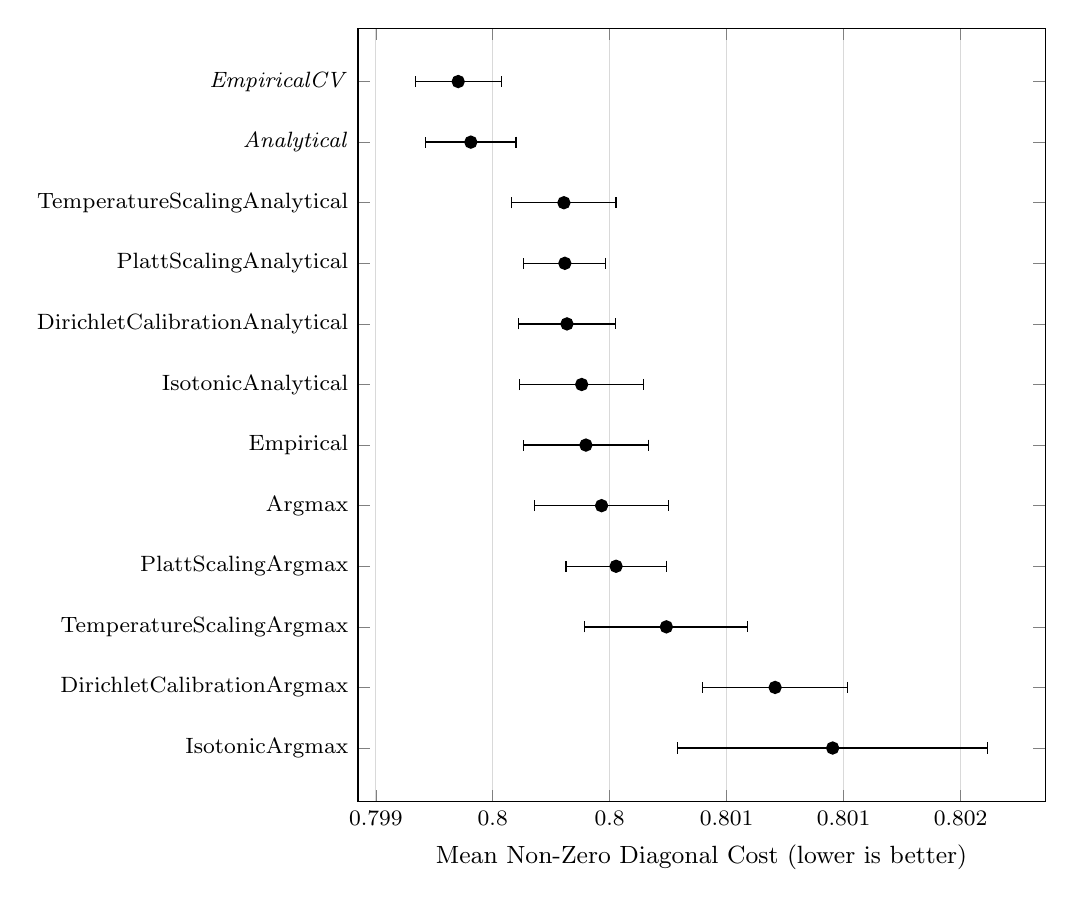
\begin{tikzpicture}
\begin{axis}[
    width=0.85\textwidth, height=11.40cm,
    xlabel={Mean Non-Zero Diagonal Cost (lower is better)},
    symbolic y coords={{EmpiricalCV},{Analytical},{TemperatureScalingAnalytical},{PlattScalingAnalytical},{DirichletCalibrationAnalytical},{IsotonicAnalytical},{Empirical},{Argmax},{PlattScalingArgmax},{TemperatureScalingArgmax},{DirichletCalibrationArgmax},{IsotonicArgmax}},
    ytick={{EmpiricalCV},{Analytical},{TemperatureScalingAnalytical},{PlattScalingAnalytical},{DirichletCalibrationAnalytical},{IsotonicAnalytical},{Empirical},{Argmax},{PlattScalingArgmax},{TemperatureScalingArgmax},{DirichletCalibrationArgmax},{IsotonicArgmax}},
    yticklabels={\textit{EmpiricalCV},\textit{Analytical},TemperatureScalingAnalytical,PlattScalingAnalytical,DirichletCalibrationAnalytical,IsotonicAnalytical,Empirical,Argmax,PlattScalingArgmax,TemperatureScalingArgmax,DirichletCalibrationArgmax,IsotonicArgmax},
    y dir=reverse,
    enlarge y limits=0.08,
    xmajorgrids=true,
    major grid style={draw=black!15, line width=0.3pt},
    scaled x ticks=false,
    xticklabel style={/pgf/number format/fixed, /pgf/number format/precision=3},
    tick label style={font=\footnotesize},
    label style={font=\small},
    every axis plot/.append style={thick},
]
\addplot[only marks, mark=*, mark size=2pt, color=black, error bars/x dir=both, error bars/x explicit, error bars/error bar style={color=black, line width=0.5pt}] coordinates { (0.799852,{EmpiricalCV}) +- (0.000183475,0) };
\addplot[only marks, mark=*, mark size=2pt, color=black, error bars/x dir=both, error bars/x explicit, error bars/error bar style={color=black, line width=0.5pt}] coordinates { (0.799906,{Analytical}) +- (0.00019296,0) };
\addplot[only marks, mark=*, mark size=2pt, color=black, error bars/x dir=both, error bars/x explicit, error bars/error bar style={color=black, line width=0.5pt}] coordinates { (0.800304,{TemperatureScalingAnalytical}) +- (0.000222498,0) };
\addplot[only marks, mark=*, mark size=2pt, color=black, error bars/x dir=both, error bars/x explicit, error bars/error bar style={color=black, line width=0.5pt}] coordinates { (0.800308,{PlattScalingAnalytical}) +- (0.00017561,0) };
\addplot[only marks, mark=*, mark size=2pt, color=black, error bars/x dir=both, error bars/x explicit, error bars/error bar style={color=black, line width=0.5pt}] coordinates { (0.800317,{DirichletCalibrationAnalytical}) +- (0.000207701,0) };
\addplot[only marks, mark=*, mark size=2pt, color=black, error bars/x dir=both, error bars/x explicit, error bars/error bar style={color=black, line width=0.5pt}] coordinates { (0.80038,{IsotonicAnalytical}) +- (0.000265909,0) };
\addplot[only marks, mark=*, mark size=2pt, color=black, error bars/x dir=both, error bars/x explicit, error bars/error bar style={color=black, line width=0.5pt}] coordinates { (0.800398,{Empirical}) +- (0.000266843,0) };
\addplot[only marks, mark=*, mark size=2pt, color=black, error bars/x dir=both, error bars/x explicit, error bars/error bar style={color=black, line width=0.5pt}] coordinates { (0.800465,{Argmax}) +- (0.00028664,0) };
\addplot[only marks, mark=*, mark size=2pt, color=black, error bars/x dir=both, error bars/x explicit, error bars/error bar style={color=black, line width=0.5pt}] coordinates { (0.800527,{PlattScalingArgmax}) +- (0.000214262,0) };
\addplot[only marks, mark=*, mark size=2pt, color=black, error bars/x dir=both, error bars/x explicit, error bars/error bar style={color=black, line width=0.5pt}] coordinates { (0.800742,{TemperatureScalingArgmax}) +- (0.000348452,0) };
\addplot[only marks, mark=*, mark size=2pt, color=black, error bars/x dir=both, error bars/x explicit, error bars/error bar style={color=black, line width=0.5pt}] coordinates { (0.801207,{DirichletCalibrationArgmax}) +- (0.000311069,0) };
\addplot[only marks, mark=*, mark size=2pt, color=black, error bars/x dir=both, error bars/x explicit, error bars/error bar style={color=black, line width=0.5pt}] coordinates { (0.801453,{IsotonicArgmax}) +- (0.000663325,0) };
\end{axis}
\end{tikzpicture}%
}
\caption{mammography: Non-Zero Diagonal Cost on TabICL (lower is better). Each dot is a strategy's mean over ten seeds with a $\pm 1$ SE horizontal bar; rows are sorted by mean, and the best strategy and any whose interval overlaps it are italicized.}%
\label{fig:ci-mammography-non-zero_diagonal_cost}
\end{figure}


\subsection{Validation label budget across empirical strategies}

The two empirical strategies differ only in the data used to choose the threshold, and that difference governs their behaviour.

Empirical tunes on the $10\%$ validation partition. Its cost win-or-tie rate is $42\%$, the lowest among the non-cost-blind strategies and below the bare analytical rule's $69\%$. The parametric calibrate-then-analytical pipelines (Platt, Temperature, Dirichlet) sit between, with win-or-tie rates of $65$, $73$, and $70\%$.

EmpiricalCV selects the threshold by five-fold cross-validation over the full $80\%$ pool, eight times the label budget of the validation split. Its cost win-or-tie rate is $87\%$, the highest in the suite. On the Asymmetric $100\times$ objective, where heavy class skew makes single-split tuning least reliable, the pooled mean-loss gap between Empirical and EmpiricalCV is widest on small datasets ($+1.90$ on $n < 10^3$ data), narrowing on medium ($+0.32$) and large ($+0.11$) data. This pattern is consistent with the validation-budget reading but does not isolate it from other dataset-size confounds.

Within the non-tuning strategies under decomposable cost objectives, the parametric calibrate-then-analytical pipelines (Platt, Temperature, Dirichlet) achieve the next-highest win-or-tie rates after EmpiricalCV\@. On individual (dataset, model) cells the parametric calibrators can match or beat EmpiricalCV\@; the per-cell numbers vary and are reported in the companion supplement.

\subsection{Non-decomposable objectives}

For the five maximization metrics ($F_1$, $F_{0.5}$, $F_2$, MCC, and G-Mean) no threshold can be computed from the metric definition alone. For $F_\beta$, for instance, the optimal classifier thresholds the conditional class probability at $F_\beta^*/(1+\beta^2)$, where $F_\beta^*$ is the optimal value of the metric and depends on the data distribution \citep{koyejo2014consistent}; for $F_1$ the threshold is $F_1^*/2$ \citep{lipton2014optimal}. The empirical family, which selects the threshold on held-out data as the consistent plug-in procedures of \citet{koyejo2014consistent} and \citet{narasimhan2014statistical} do, is therefore the only family here that targets these metrics directly.

Pooled across maximization metrics, EmpiricalCV wins or ties $99.9\%$ of cells, Empirical $73\%$, and Argmax $45\%$. Calibrate-then-Argmax strategies sit near Argmax ($28$ to $38\%$): a monotone calibrator does not move the $\arg\max$ of a symmetric-threshold decision.

Figure~\ref{fig:ci-adult-mcc} shows a representative cell, \textit{adult} with TabM on MCC\@: the empirical strategies lead, Argmax is close behind, and the calibrate-then-Argmax strategies sit a few points lower.

% Auto-generated by experiments.analysis.generate_ci_plots --- do not edit.
\begin{figure}[H]
\centering
\adjustbox{max width=\textwidth}{%
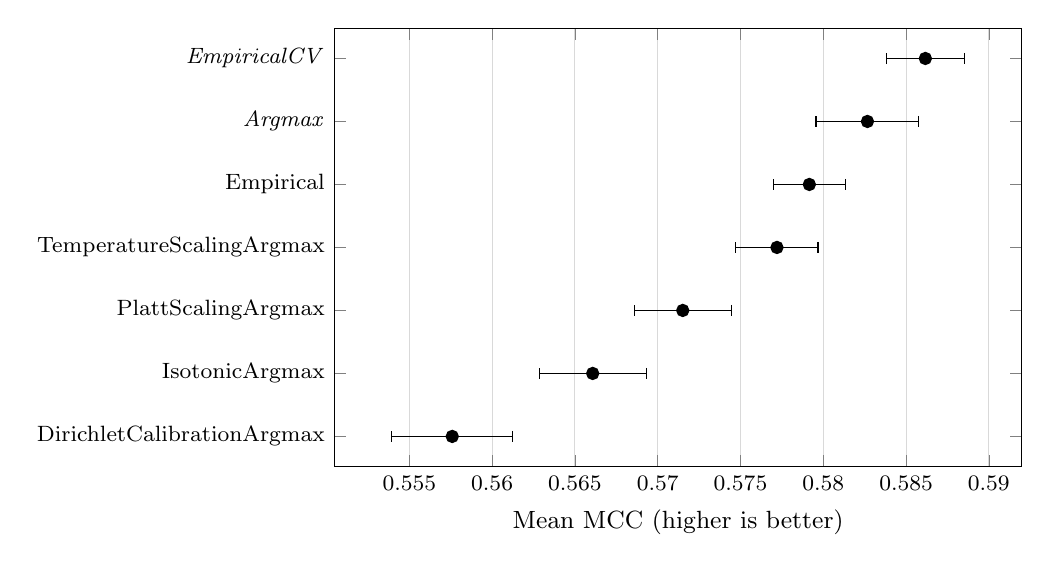
\begin{tikzpicture}
\begin{axis}[
    width=0.85\textwidth, height=7.15cm,
    xlabel={Mean MCC (higher is better)},
    symbolic y coords={{EmpiricalCV},{Argmax},{Empirical},{TemperatureScalingArgmax},{PlattScalingArgmax},{IsotonicArgmax},{DirichletCalibrationArgmax}},
    ytick={{EmpiricalCV},{Argmax},{Empirical},{TemperatureScalingArgmax},{PlattScalingArgmax},{IsotonicArgmax},{DirichletCalibrationArgmax}},
    yticklabels={\textit{EmpiricalCV},\textit{Argmax},Empirical,TemperatureScalingArgmax,PlattScalingArgmax,IsotonicArgmax,DirichletCalibrationArgmax},
    y dir=reverse,
    enlarge y limits=0.08,
    xmajorgrids=true,
    major grid style={draw=black!15, line width=0.3pt},
    scaled x ticks=false,
    xticklabel style={/pgf/number format/fixed, /pgf/number format/precision=3},
    tick label style={font=\footnotesize},
    label style={font=\small},
    every axis plot/.append style={thick},
]
\addplot[only marks, mark=*, mark size=2pt, color=black, error bars/x dir=both, error bars/x explicit, error bars/error bar style={color=black, line width=0.5pt}] coordinates { (0.586167,{EmpiricalCV}) +- (0.00235058,0) };
\addplot[only marks, mark=*, mark size=2pt, color=black, error bars/x dir=both, error bars/x explicit, error bars/error bar style={color=black, line width=0.5pt}] coordinates { (0.582668,{Argmax}) +- (0.00310402,0) };
\addplot[only marks, mark=*, mark size=2pt, color=black, error bars/x dir=both, error bars/x explicit, error bars/error bar style={color=black, line width=0.5pt}] coordinates { (0.57916,{Empirical}) +- (0.00218688,0) };
\addplot[only marks, mark=*, mark size=2pt, color=black, error bars/x dir=both, error bars/x explicit, error bars/error bar style={color=black, line width=0.5pt}] coordinates { (0.577204,{TemperatureScalingArgmax}) +- (0.00247722,0) };
\addplot[only marks, mark=*, mark size=2pt, color=black, error bars/x dir=both, error bars/x explicit, error bars/error bar style={color=black, line width=0.5pt}] coordinates { (0.571515,{PlattScalingArgmax}) +- (0.00292098,0) };
\addplot[only marks, mark=*, mark size=2pt, color=black, error bars/x dir=both, error bars/x explicit, error bars/error bar style={color=black, line width=0.5pt}] coordinates { (0.566076,{IsotonicArgmax}) +- (0.00322504,0) };
\addplot[only marks, mark=*, mark size=2pt, color=black, error bars/x dir=both, error bars/x explicit, error bars/error bar style={color=black, line width=0.5pt}] coordinates { (0.557592,{DirichletCalibrationArgmax}) +- (0.00365129,0) };
\end{axis}
\end{tikzpicture}%
}
\caption{adult: MCC on TabM (higher is better). Each dot is a strategy's mean over ten seeds with a $\pm 1$ SE horizontal bar; rows are sorted by mean, and the best strategy and any whose interval overlaps it are italicized.}%
\label{fig:ci-adult-mcc}
\end{figure}


Figures~\ref{fig:win-counts-binary-cost} and~\ref{fig:win-counts-binary-max} give the per-strategy win and tie rates under the $\pm 1$ SE overlap rule, broken out by base classifier and by dataset size and imbalance bucket; the figure captions document the reading convention and the bootstrap half-width.

% Auto-generated by experiments.analysis.generate_win_counts --- do not edit.
\begin{figure}[H]
\centering
\adjustbox{max width=\textwidth}{%
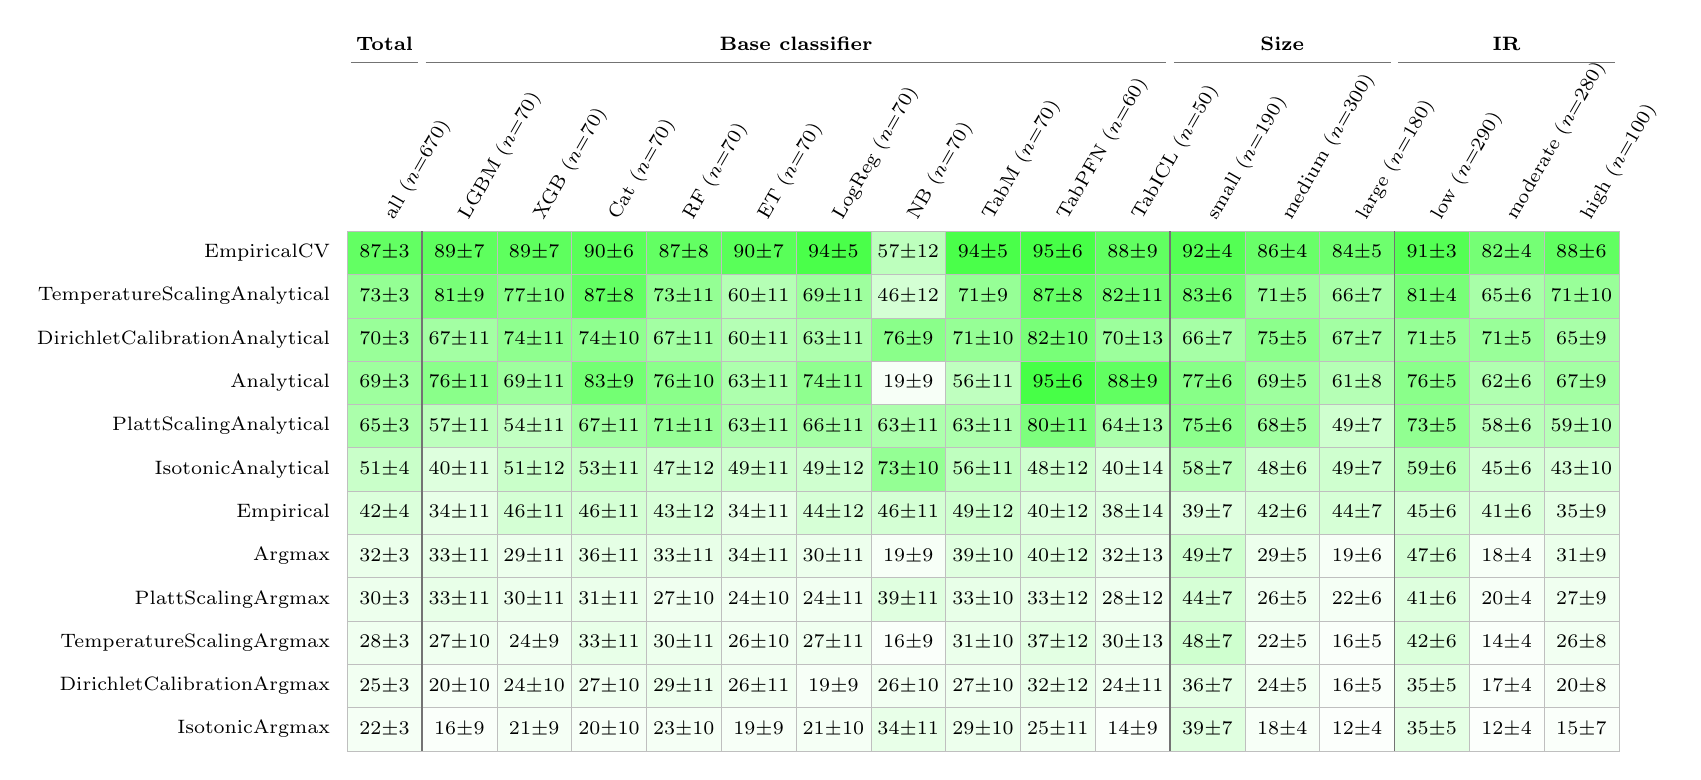
\begin{tikzpicture}[
    x=0.95cm, y=0.55cm,
    cell/.style={rectangle, draw=black!25, line width=0.2pt,
        minimum width=0.95cm, minimum height=0.55cm,
        anchor=center, font=\scriptsize, inner sep=0pt},
    rowlbl/.style={font=\scriptsize, anchor=east},
    collbl/.style={font=\scriptsize, anchor=west, rotate=60},
    grouplbl/.style={font=\scriptsize\bfseries, anchor=south},
    sep/.style={draw=black!55, line width=0.5pt},
]
\node[cell, fill=green!61] at (1, 12) {$87{\pm}3$};
\node[cell, fill=green!63] at (2, 12) {$89{\pm}7$};
\node[cell, fill=green!63] at (3, 12) {$89{\pm}7$};
\node[cell, fill=green!65] at (4, 12) {$90{\pm}6$};
\node[cell, fill=green!61] at (5, 12) {$87{\pm}8$};
\node[cell, fill=green!65] at (6, 12) {$90{\pm}7$};
\node[cell, fill=green!71] at (7, 12) {$94{\pm}5$};
\node[cell, fill=green!26] at (8, 12) {$57{\pm}12$};
\node[cell, fill=green!71] at (9, 12) {$94{\pm}5$};
\node[cell, fill=green!72] at (10, 12) {$95{\pm}6$};
\node[cell, fill=green!62] at (11, 12) {$88{\pm}9$};
\node[cell, fill=green!67] at (12, 12) {$92{\pm}4$};
\node[cell, fill=green!59] at (13, 12) {$86{\pm}4$};
\node[cell, fill=green!57] at (14, 12) {$84{\pm}5$};
\node[cell, fill=green!67] at (15, 12) {$91{\pm}3$};
\node[cell, fill=green!54] at (16, 12) {$82{\pm}4$};
\node[cell, fill=green!62] at (17, 12) {$88{\pm}6$};
\node[cell, fill=green!42] at (1, 11) {$73{\pm}3$};
\node[cell, fill=green!53] at (2, 11) {$81{\pm}9$};
\node[cell, fill=green!48] at (3, 11) {$77{\pm}10$};
\node[cell, fill=green!61] at (4, 11) {$87{\pm}8$};
\node[cell, fill=green!42] at (5, 11) {$73{\pm}11$};
\node[cell, fill=green!29] at (6, 11) {$60{\pm}11$};
\node[cell, fill=green!38] at (7, 11) {$69{\pm}11$};
\node[cell, fill=green!17] at (8, 11) {$46{\pm}12$};
\node[cell, fill=green!41] at (9, 11) {$71{\pm}9$};
\node[cell, fill=green!60] at (10, 11) {$87{\pm}8$};
\node[cell, fill=green!54] at (11, 11) {$82{\pm}11$};
\node[cell, fill=green!55] at (12, 11) {$83{\pm}6$};
\node[cell, fill=green!40] at (13, 11) {$71{\pm}5$};
\node[cell, fill=green!34] at (14, 11) {$66{\pm}7$};
\node[cell, fill=green!53] at (15, 11) {$81{\pm}4$};
\node[cell, fill=green!34] at (16, 11) {$65{\pm}6$};
\node[cell, fill=green!40] at (17, 11) {$71{\pm}10$};
\node[cell, fill=green!40] at (1, 10) {$70{\pm}3$};
\node[cell, fill=green!36] at (2, 10) {$67{\pm}11$};
\node[cell, fill=green!44] at (3, 10) {$74{\pm}11$};
\node[cell, fill=green!44] at (4, 10) {$74{\pm}10$};
\node[cell, fill=green!36] at (5, 10) {$67{\pm}11$};
\node[cell, fill=green!29] at (6, 10) {$60{\pm}11$};
\node[cell, fill=green!32] at (7, 10) {$63{\pm}11$};
\node[cell, fill=green!46] at (8, 10) {$76{\pm}9$};
\node[cell, fill=green!41] at (9, 10) {$71{\pm}10$};
\node[cell, fill=green!53] at (10, 10) {$82{\pm}10$};
\node[cell, fill=green!39] at (11, 10) {$70{\pm}13$};
\node[cell, fill=green!35] at (12, 10) {$66{\pm}7$};
\node[cell, fill=green!45] at (13, 10) {$75{\pm}5$};
\node[cell, fill=green!36] at (14, 10) {$67{\pm}7$};
\node[cell, fill=green!41] at (15, 10) {$71{\pm}5$};
\node[cell, fill=green!40] at (16, 10) {$71{\pm}5$};
\node[cell, fill=green!34] at (17, 10) {$65{\pm}9$};
\node[cell, fill=green!38] at (1, 9) {$69{\pm}3$};
\node[cell, fill=green!46] at (2, 9) {$76{\pm}11$};
\node[cell, fill=green!38] at (3, 9) {$69{\pm}11$};
\node[cell, fill=green!55] at (4, 9) {$83{\pm}9$};
\node[cell, fill=green!46] at (5, 9) {$76{\pm}10$};
\node[cell, fill=green!32] at (6, 9) {$63{\pm}11$};
\node[cell, fill=green!44] at (7, 9) {$74{\pm}11$};
\node[cell, fill=green!3] at (8, 9) {$19{\pm}9$};
\node[cell, fill=green!25] at (9, 9) {$56{\pm}11$};
\node[cell, fill=green!72] at (10, 9) {$95{\pm}6$};
\node[cell, fill=green!62] at (11, 9) {$88{\pm}9$};
\node[cell, fill=green!47] at (12, 9) {$77{\pm}6$};
\node[cell, fill=green!38] at (13, 9) {$69{\pm}5$};
\node[cell, fill=green!29] at (14, 9) {$61{\pm}8$};
\node[cell, fill=green!46] at (15, 9) {$76{\pm}5$};
\node[cell, fill=green!31] at (16, 9) {$62{\pm}6$};
\node[cell, fill=green!36] at (17, 9) {$67{\pm}9$};
\node[cell, fill=green!33] at (1, 8) {$65{\pm}3$};
\node[cell, fill=green!26] at (2, 8) {$57{\pm}11$};
\node[cell, fill=green!24] at (3, 8) {$54{\pm}11$};
\node[cell, fill=green!36] at (4, 8) {$67{\pm}11$};
\node[cell, fill=green!41] at (5, 8) {$71{\pm}11$};
\node[cell, fill=green!32] at (6, 8) {$63{\pm}11$};
\node[cell, fill=green!35] at (7, 8) {$66{\pm}11$};
\node[cell, fill=green!32] at (8, 8) {$63{\pm}11$};
\node[cell, fill=green!32] at (9, 8) {$63{\pm}11$};
\node[cell, fill=green!51] at (10, 8) {$80{\pm}11$};
\node[cell, fill=green!33] at (11, 8) {$64{\pm}13$};
\node[cell, fill=green!45] at (12, 8) {$75{\pm}6$};
\node[cell, fill=green!37] at (13, 8) {$68{\pm}5$};
\node[cell, fill=green!19] at (14, 8) {$49{\pm}7$};
\node[cell, fill=green!43] at (15, 8) {$73{\pm}5$};
\node[cell, fill=green!27] at (16, 8) {$58{\pm}6$};
\node[cell, fill=green!28] at (17, 8) {$59{\pm}10$};
\node[cell, fill=green!21] at (1, 7) {$51{\pm}4$};
\node[cell, fill=green!13] at (2, 7) {$40{\pm}11$};
\node[cell, fill=green!21] at (3, 7) {$51{\pm}12$};
\node[cell, fill=green!22] at (4, 7) {$53{\pm}11$};
\node[cell, fill=green!18] at (5, 7) {$47{\pm}12$};
\node[cell, fill=green!19] at (6, 7) {$49{\pm}11$};
\node[cell, fill=green!19] at (7, 7) {$49{\pm}12$};
\node[cell, fill=green!42] at (8, 7) {$73{\pm}10$};
\node[cell, fill=green!25] at (9, 7) {$56{\pm}11$};
\node[cell, fill=green!19] at (10, 7) {$48{\pm}12$};
\node[cell, fill=green!13] at (11, 7) {$40{\pm}14$};
\node[cell, fill=green!27] at (12, 7) {$58{\pm}7$};
\node[cell, fill=green!18] at (13, 7) {$48{\pm}6$};
\node[cell, fill=green!19] at (14, 7) {$49{\pm}7$};
\node[cell, fill=green!28] at (15, 7) {$59{\pm}6$};
\node[cell, fill=green!16] at (16, 7) {$45{\pm}6$};
\node[cell, fill=green!15] at (17, 7) {$43{\pm}10$};
\node[cell, fill=green!14] at (1, 6) {$42{\pm}4$};
\node[cell, fill=green!9] at (2, 6) {$34{\pm}11$};
\node[cell, fill=green!17] at (3, 6) {$46{\pm}11$};
\node[cell, fill=green!17] at (4, 6) {$46{\pm}11$};
\node[cell, fill=green!15] at (5, 6) {$43{\pm}12$};
\node[cell, fill=green!9] at (6, 6) {$34{\pm}11$};
\node[cell, fill=green!16] at (7, 6) {$44{\pm}12$};
\node[cell, fill=green!17] at (8, 6) {$46{\pm}11$};
\node[cell, fill=green!19] at (9, 6) {$49{\pm}12$};
\node[cell, fill=green!13] at (10, 6) {$40{\pm}12$};
\node[cell, fill=green!12] at (11, 6) {$38{\pm}14$};
\node[cell, fill=green!12] at (12, 6) {$39{\pm}7$};
\node[cell, fill=green!14] at (13, 6) {$42{\pm}6$};
\node[cell, fill=green!16] at (14, 6) {$44{\pm}7$};
\node[cell, fill=green!16] at (15, 6) {$45{\pm}6$};
\node[cell, fill=green!14] at (16, 6) {$41{\pm}6$};
\node[cell, fill=green!10] at (17, 6) {$35{\pm}9$};
\node[cell, fill=green!8] at (1, 5) {$32{\pm}3$};
\node[cell, fill=green!9] at (2, 5) {$33{\pm}11$};
\node[cell, fill=green!7] at (3, 5) {$29{\pm}11$};
\node[cell, fill=green!10] at (4, 5) {$36{\pm}11$};
\node[cell, fill=green!9] at (5, 5) {$33{\pm}11$};
\node[cell, fill=green!9] at (6, 5) {$34{\pm}11$};
\node[cell, fill=green!7] at (7, 5) {$30{\pm}11$};
\node[cell, fill=green!3] at (8, 5) {$19{\pm}9$};
\node[cell, fill=green!12] at (9, 5) {$39{\pm}10$};
\node[cell, fill=green!13] at (10, 5) {$40{\pm}12$};
\node[cell, fill=green!8] at (11, 5) {$32{\pm}13$};
\node[cell, fill=green!19] at (12, 5) {$49{\pm}7$};
\node[cell, fill=green!7] at (13, 5) {$29{\pm}5$};
\node[cell, fill=green!3] at (14, 5) {$19{\pm}6$};
\node[cell, fill=green!17] at (15, 5) {$47{\pm}6$};
\node[cell, fill=green!3] at (16, 5) {$18{\pm}4$};
\node[cell, fill=green!8] at (17, 5) {$31{\pm}9$};
\node[cell, fill=green!7] at (1, 4) {$30{\pm}3$};
\node[cell, fill=green!9] at (2, 4) {$33{\pm}11$};
\node[cell, fill=green!7] at (3, 4) {$30{\pm}11$};
\node[cell, fill=green!8] at (4, 4) {$31{\pm}11$};
\node[cell, fill=green!6] at (5, 4) {$27{\pm}10$};
\node[cell, fill=green!5] at (6, 4) {$24{\pm}10$};
\node[cell, fill=green!5] at (7, 4) {$24{\pm}11$};
\node[cell, fill=green!12] at (8, 4) {$39{\pm}11$};
\node[cell, fill=green!9] at (9, 4) {$33{\pm}10$};
\node[cell, fill=green!9] at (10, 4) {$33{\pm}12$};
\node[cell, fill=green!6] at (11, 4) {$28{\pm}12$};
\node[cell, fill=green!16] at (12, 4) {$44{\pm}7$};
\node[cell, fill=green!6] at (13, 4) {$26{\pm}5$};
\node[cell, fill=green!4] at (14, 4) {$22{\pm}6$};
\node[cell, fill=green!13] at (15, 4) {$41{\pm}6$};
\node[cell, fill=green!3] at (16, 4) {$20{\pm}4$};
\node[cell, fill=green!6] at (17, 4) {$27{\pm}9$};
\node[cell, fill=green!6] at (1, 3) {$28{\pm}3$};
\node[cell, fill=green!6] at (2, 3) {$27{\pm}10$};
\node[cell, fill=green!5] at (3, 3) {$24{\pm}9$};
\node[cell, fill=green!9] at (4, 3) {$33{\pm}11$};
\node[cell, fill=green!7] at (5, 3) {$30{\pm}11$};
\node[cell, fill=green!5] at (6, 3) {$26{\pm}10$};
\node[cell, fill=green!6] at (7, 3) {$27{\pm}11$};
\node[cell, fill=green!2] at (8, 3) {$16{\pm}9$};
\node[cell, fill=green!8] at (9, 3) {$31{\pm}10$};
\node[cell, fill=green!11] at (10, 3) {$37{\pm}12$};
\node[cell, fill=green!7] at (11, 3) {$30{\pm}13$};
\node[cell, fill=green!19] at (12, 3) {$48{\pm}7$};
\node[cell, fill=green!4] at (13, 3) {$22{\pm}5$};
\node[cell, fill=green!2] at (14, 3) {$16{\pm}5$};
\node[cell, fill=green!14] at (15, 3) {$42{\pm}6$};
\node[cell, fill=green!2] at (16, 3) {$14{\pm}4$};
\node[cell, fill=green!5] at (17, 3) {$26{\pm}8$};
\node[cell, fill=green!5] at (1, 2) {$25{\pm}3$};
\node[cell, fill=green!3] at (2, 2) {$20{\pm}10$};
\node[cell, fill=green!5] at (3, 2) {$24{\pm}10$};
\node[cell, fill=green!6] at (4, 2) {$27{\pm}10$};
\node[cell, fill=green!7] at (5, 2) {$29{\pm}11$};
\node[cell, fill=green!5] at (6, 2) {$26{\pm}11$};
\node[cell, fill=green!3] at (7, 2) {$19{\pm}9$};
\node[cell, fill=green!5] at (8, 2) {$26{\pm}10$};
\node[cell, fill=green!6] at (9, 2) {$27{\pm}10$};
\node[cell, fill=green!8] at (10, 2) {$32{\pm}12$};
\node[cell, fill=green!5] at (11, 2) {$24{\pm}11$};
\node[cell, fill=green!10] at (12, 2) {$36{\pm}7$};
\node[cell, fill=green!5] at (13, 2) {$24{\pm}5$};
\node[cell, fill=green!2] at (14, 2) {$16{\pm}5$};
\node[cell, fill=green!10] at (15, 2) {$35{\pm}5$};
\node[cell, fill=green!2] at (16, 2) {$17{\pm}4$};
\node[cell, fill=green!3] at (17, 2) {$20{\pm}8$};
\node[cell, fill=green!4] at (1, 1) {$22{\pm}3$};
\node[cell, fill=green!2] at (2, 1) {$16{\pm}9$};
\node[cell, fill=green!4] at (3, 1) {$21{\pm}9$};
\node[cell, fill=green!3] at (4, 1) {$20{\pm}10$};
\node[cell, fill=green!4] at (5, 1) {$23{\pm}10$};
\node[cell, fill=green!3] at (6, 1) {$19{\pm}9$};
\node[cell, fill=green!4] at (7, 1) {$21{\pm}10$};
\node[cell, fill=green!9] at (8, 1) {$34{\pm}11$};
\node[cell, fill=green!7] at (9, 1) {$29{\pm}10$};
\node[cell, fill=green!5] at (10, 1) {$25{\pm}11$};
\node[cell, fill=green!2] at (11, 1) {$14{\pm}9$};
\node[cell, fill=green!12] at (12, 1) {$39{\pm}7$};
\node[cell, fill=green!3] at (13, 1) {$18{\pm}4$};
\node[cell, fill=green!1] at (14, 1) {$12{\pm}4$};
\node[cell, fill=green!10] at (15, 1) {$35{\pm}5$};
\node[cell, fill=green!1] at (16, 1) {$12{\pm}4$};
\node[cell, fill=green!2] at (17, 1) {$15{\pm}7$};
\node[rowlbl] at (0.4, 12) {EmpiricalCV};
\node[rowlbl] at (0.4, 11) {TemperatureScalingAnalytical};
\node[rowlbl] at (0.4, 10) {DirichletCalibrationAnalytical};
\node[rowlbl] at (0.4, 9) {Analytical};
\node[rowlbl] at (0.4, 8) {PlattScalingAnalytical};
\node[rowlbl] at (0.4, 7) {IsotonicAnalytical};
\node[rowlbl] at (0.4, 6) {Empirical};
\node[rowlbl] at (0.4, 5) {Argmax};
\node[rowlbl] at (0.4, 4) {PlattScalingArgmax};
\node[rowlbl] at (0.4, 3) {TemperatureScalingArgmax};
\node[rowlbl] at (0.4, 2) {DirichletCalibrationArgmax};
\node[rowlbl] at (0.4, 1) {IsotonicArgmax};
\node[collbl] at (1, 12.6) {all ($n{=}670$)};
\node[collbl] at (2, 12.6) {LGBM ($n{=}70$)};
\node[collbl] at (3, 12.6) {XGB ($n{=}70$)};
\node[collbl] at (4, 12.6) {Cat ($n{=}70$)};
\node[collbl] at (5, 12.6) {RF ($n{=}70$)};
\node[collbl] at (6, 12.6) {ET ($n{=}70$)};
\node[collbl] at (7, 12.6) {LogReg ($n{=}70$)};
\node[collbl] at (8, 12.6) {NB ($n{=}70$)};
\node[collbl] at (9, 12.6) {TabM ($n{=}70$)};
\node[collbl] at (10, 12.6) {TabPFN ($n{=}60$)};
\node[collbl] at (11, 12.6) {TabICL ($n{=}50$)};
\node[collbl] at (12, 12.6) {small ($n{=}190$)};
\node[collbl] at (13, 12.6) {medium ($n{=}300$)};
\node[collbl] at (14, 12.6) {large ($n{=}180$)};
\node[collbl] at (15, 12.6) {low ($n{=}290$)};
\node[collbl] at (16, 12.6) {moderate ($n{=}280$)};
\node[collbl] at (17, 12.6) {high ($n{=}100$)};
\draw[black!55, line width=0.5pt] (0.55, 16.4) -- (1.45, 16.4);
\node[grouplbl] at (1.0, 16.45) {Total};
\draw[black!55, line width=0.5pt] (1.55, 16.4) -- (11.45, 16.4);
\node[grouplbl] at (6.5, 16.45) {Base classifier};
\draw[black!55, line width=0.5pt] (11.55, 16.4) -- (14.45, 16.4);
\node[grouplbl] at (13.0, 16.45) {Size};
\draw[black!55, line width=0.5pt] (14.55, 16.4) -- (17.45, 16.4);
\node[grouplbl] at (16.0, 16.45) {IR};
\draw[sep] (1.5, 0.5) -- (1.5, 12.5);
\draw[sep] (11.5, 0.5) -- (11.5, 12.5);
\draw[sep] (14.5, 0.5) -- (14.5, 12.5);
\end{tikzpicture}%
}
\caption{Per-strategy win/tie rates on binary cost-matrix objectives. Each cell reads ``$r{\pm}H$'': $r$ is the percentage of (dataset, model, objective) cells in the slice where the strategy won or tied the per-row best under the $\pm 1$ SE overlap rule, and $H$ is the half-width of a 95\% cluster-bootstrap confidence interval for $r$ (percentage points). Shading is a quadratic ($\mathrm{rate}^2$) scale of $r$. Strategies are sorted by overall win rate; ``$n$'' under each column header is the maximum applicable cell count for that slice.}%
\label{fig:win-counts-binary-cost}
\end{figure}


% Auto-generated by experiments.analysis.generate_win_counts --- do not edit.
\begin{figure}[H]
\centering
\adjustbox{max width=\textwidth}{%
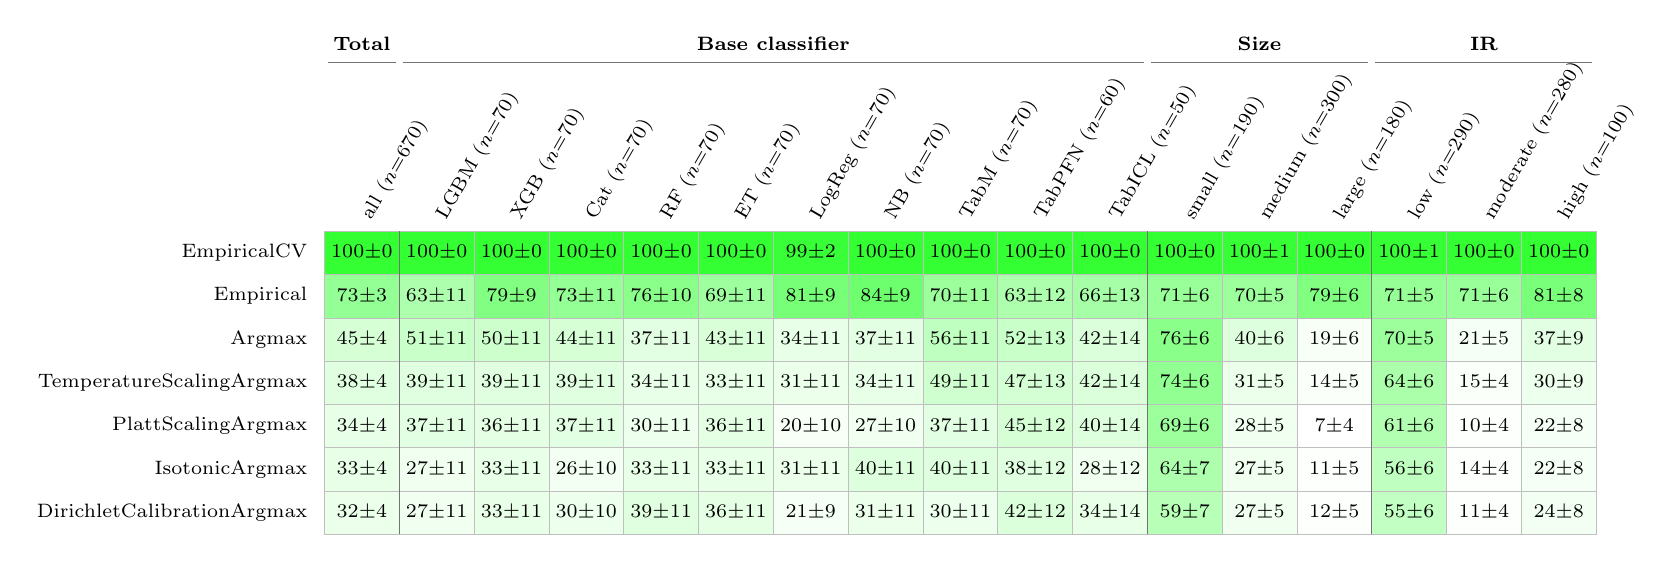
\begin{tikzpicture}[
    x=0.95cm, y=0.55cm,
    cell/.style={rectangle, draw=black!25, line width=0.2pt,
        minimum width=0.95cm, minimum height=0.55cm,
        anchor=center, font=\scriptsize, inner sep=0pt},
    rowlbl/.style={font=\scriptsize, anchor=east},
    collbl/.style={font=\scriptsize, anchor=west, rotate=60},
    grouplbl/.style={font=\scriptsize\bfseries, anchor=south},
    sep/.style={draw=black!55, line width=0.5pt},
]
\node[cell, fill=green!80] at (1, 7) {$100{\pm}0$};
\node[cell, fill=green!80] at (2, 7) {$100{\pm}0$};
\node[cell, fill=green!80] at (3, 7) {$100{\pm}0$};
\node[cell, fill=green!80] at (4, 7) {$100{\pm}0$};
\node[cell, fill=green!80] at (5, 7) {$100{\pm}0$};
\node[cell, fill=green!80] at (6, 7) {$100{\pm}0$};
\node[cell, fill=green!78] at (7, 7) {$99{\pm}2$};
\node[cell, fill=green!80] at (8, 7) {$100{\pm}0$};
\node[cell, fill=green!80] at (9, 7) {$100{\pm}0$};
\node[cell, fill=green!80] at (10, 7) {$100{\pm}0$};
\node[cell, fill=green!80] at (11, 7) {$100{\pm}0$};
\node[cell, fill=green!80] at (12, 7) {$100{\pm}0$};
\node[cell, fill=green!79] at (13, 7) {$100{\pm}1$};
\node[cell, fill=green!80] at (14, 7) {$100{\pm}0$};
\node[cell, fill=green!79] at (15, 7) {$100{\pm}1$};
\node[cell, fill=green!80] at (16, 7) {$100{\pm}0$};
\node[cell, fill=green!80] at (17, 7) {$100{\pm}0$};
\node[cell, fill=green!42] at (1, 6) {$73{\pm}3$};
\node[cell, fill=green!32] at (2, 6) {$63{\pm}11$};
\node[cell, fill=green!49] at (3, 6) {$79{\pm}9$};
\node[cell, fill=green!42] at (4, 6) {$73{\pm}11$};
\node[cell, fill=green!46] at (5, 6) {$76{\pm}10$};
\node[cell, fill=green!38] at (6, 6) {$69{\pm}11$};
\node[cell, fill=green!53] at (7, 6) {$81{\pm}9$};
\node[cell, fill=green!57] at (8, 6) {$84{\pm}9$};
\node[cell, fill=green!39] at (9, 6) {$70{\pm}11$};
\node[cell, fill=green!32] at (10, 6) {$63{\pm}12$};
\node[cell, fill=green!35] at (11, 6) {$66{\pm}13$};
\node[cell, fill=green!40] at (12, 6) {$71{\pm}6$};
\node[cell, fill=green!39] at (13, 6) {$70{\pm}5$};
\node[cell, fill=green!50] at (14, 6) {$79{\pm}6$};
\node[cell, fill=green!41] at (15, 6) {$71{\pm}5$};
\node[cell, fill=green!40] at (16, 6) {$71{\pm}6$};
\node[cell, fill=green!52] at (17, 6) {$81{\pm}8$};
\node[cell, fill=green!16] at (1, 5) {$45{\pm}4$};
\node[cell, fill=green!21] at (2, 5) {$51{\pm}11$};
\node[cell, fill=green!20] at (3, 5) {$50{\pm}11$};
\node[cell, fill=green!16] at (4, 5) {$44{\pm}11$};
\node[cell, fill=green!11] at (5, 5) {$37{\pm}11$};
\node[cell, fill=green!15] at (6, 5) {$43{\pm}11$};
\node[cell, fill=green!9] at (7, 5) {$34{\pm}11$};
\node[cell, fill=green!11] at (8, 5) {$37{\pm}11$};
\node[cell, fill=green!25] at (9, 5) {$56{\pm}11$};
\node[cell, fill=green!21] at (10, 5) {$52{\pm}13$};
\node[cell, fill=green!14] at (11, 5) {$42{\pm}14$};
\node[cell, fill=green!46] at (12, 5) {$76{\pm}6$};
\node[cell, fill=green!13] at (13, 5) {$40{\pm}6$};
\node[cell, fill=green!3] at (14, 5) {$19{\pm}6$};
\node[cell, fill=green!39] at (15, 5) {$70{\pm}5$};
\node[cell, fill=green!4] at (16, 5) {$21{\pm}5$};
\node[cell, fill=green!11] at (17, 5) {$37{\pm}9$};
\node[cell, fill=green!12] at (1, 4) {$38{\pm}4$};
\node[cell, fill=green!12] at (2, 4) {$39{\pm}11$};
\node[cell, fill=green!12] at (3, 4) {$39{\pm}11$};
\node[cell, fill=green!12] at (4, 4) {$39{\pm}11$};
\node[cell, fill=green!9] at (5, 4) {$34{\pm}11$};
\node[cell, fill=green!9] at (6, 4) {$33{\pm}11$};
\node[cell, fill=green!8] at (7, 4) {$31{\pm}11$};
\node[cell, fill=green!9] at (8, 4) {$34{\pm}11$};
\node[cell, fill=green!19] at (9, 4) {$49{\pm}11$};
\node[cell, fill=green!17] at (10, 4) {$47{\pm}13$};
\node[cell, fill=green!14] at (11, 4) {$42{\pm}14$};
\node[cell, fill=green!43] at (12, 4) {$74{\pm}6$};
\node[cell, fill=green!8] at (13, 4) {$31{\pm}5$};
\node[cell, fill=green!2] at (14, 4) {$14{\pm}5$};
\node[cell, fill=green!33] at (15, 4) {$64{\pm}6$};
\node[cell, fill=green!2] at (16, 4) {$15{\pm}4$};
\node[cell, fill=green!7] at (17, 4) {$30{\pm}9$};
\node[cell, fill=green!9] at (1, 3) {$34{\pm}4$};
\node[cell, fill=green!11] at (2, 3) {$37{\pm}11$};
\node[cell, fill=green!10] at (3, 3) {$36{\pm}11$};
\node[cell, fill=green!11] at (4, 3) {$37{\pm}11$};
\node[cell, fill=green!7] at (5, 3) {$30{\pm}11$};
\node[cell, fill=green!10] at (6, 3) {$36{\pm}11$};
\node[cell, fill=green!3] at (7, 3) {$20{\pm}10$};
\node[cell, fill=green!6] at (8, 3) {$27{\pm}10$};
\node[cell, fill=green!11] at (9, 3) {$37{\pm}11$};
\node[cell, fill=green!16] at (10, 3) {$45{\pm}12$};
\node[cell, fill=green!13] at (11, 3) {$40{\pm}14$};
\node[cell, fill=green!39] at (12, 3) {$69{\pm}6$};
\node[cell, fill=green!6] at (13, 3) {$28{\pm}5$};
\node[cell, fill=green!0] at (14, 3) {$7{\pm}4$};
\node[cell, fill=green!30] at (15, 3) {$61{\pm}6$};
\node[cell, fill=green!1] at (16, 3) {$10{\pm}4$};
\node[cell, fill=green!4] at (17, 3) {$22{\pm}8$};
\node[cell, fill=green!9] at (1, 2) {$33{\pm}4$};
\node[cell, fill=green!6] at (2, 2) {$27{\pm}11$};
\node[cell, fill=green!9] at (3, 2) {$33{\pm}11$};
\node[cell, fill=green!5] at (4, 2) {$26{\pm}10$};
\node[cell, fill=green!9] at (5, 2) {$33{\pm}11$};
\node[cell, fill=green!9] at (6, 2) {$33{\pm}11$};
\node[cell, fill=green!8] at (7, 2) {$31{\pm}11$};
\node[cell, fill=green!13] at (8, 2) {$40{\pm}11$};
\node[cell, fill=green!13] at (9, 2) {$40{\pm}11$};
\node[cell, fill=green!12] at (10, 2) {$38{\pm}12$};
\node[cell, fill=green!6] at (11, 2) {$28{\pm}12$};
\node[cell, fill=green!32] at (12, 2) {$64{\pm}7$};
\node[cell, fill=green!6] at (13, 2) {$27{\pm}5$};
\node[cell, fill=green!1] at (14, 2) {$11{\pm}5$};
\node[cell, fill=green!25] at (15, 2) {$56{\pm}6$};
\node[cell, fill=green!1] at (16, 2) {$14{\pm}4$};
\node[cell, fill=green!4] at (17, 2) {$22{\pm}8$};
\node[cell, fill=green!8] at (1, 1) {$32{\pm}4$};
\node[cell, fill=green!6] at (2, 1) {$27{\pm}11$};
\node[cell, fill=green!9] at (3, 1) {$33{\pm}11$};
\node[cell, fill=green!7] at (4, 1) {$30{\pm}10$};
\node[cell, fill=green!12] at (5, 1) {$39{\pm}11$};
\node[cell, fill=green!10] at (6, 1) {$36{\pm}11$};
\node[cell, fill=green!4] at (7, 1) {$21{\pm}9$};
\node[cell, fill=green!8] at (8, 1) {$31{\pm}11$};
\node[cell, fill=green!7] at (9, 1) {$30{\pm}11$};
\node[cell, fill=green!14] at (10, 1) {$42{\pm}12$};
\node[cell, fill=green!9] at (11, 1) {$34{\pm}14$};
\node[cell, fill=green!28] at (12, 1) {$59{\pm}7$};
\node[cell, fill=green!6] at (13, 1) {$27{\pm}5$};
\node[cell, fill=green!1] at (14, 1) {$12{\pm}5$};
\node[cell, fill=green!24] at (15, 1) {$55{\pm}6$};
\node[cell, fill=green!1] at (16, 1) {$11{\pm}4$};
\node[cell, fill=green!5] at (17, 1) {$24{\pm}8$};
\node[rowlbl] at (0.4, 7) {EmpiricalCV};
\node[rowlbl] at (0.4, 6) {Empirical};
\node[rowlbl] at (0.4, 5) {Argmax};
\node[rowlbl] at (0.4, 4) {TemperatureScalingArgmax};
\node[rowlbl] at (0.4, 3) {PlattScalingArgmax};
\node[rowlbl] at (0.4, 2) {IsotonicArgmax};
\node[rowlbl] at (0.4, 1) {DirichletCalibrationArgmax};
\node[collbl] at (1, 7.6) {all ($n{=}670$)};
\node[collbl] at (2, 7.6) {LGBM ($n{=}70$)};
\node[collbl] at (3, 7.6) {XGB ($n{=}70$)};
\node[collbl] at (4, 7.6) {Cat ($n{=}70$)};
\node[collbl] at (5, 7.6) {RF ($n{=}70$)};
\node[collbl] at (6, 7.6) {ET ($n{=}70$)};
\node[collbl] at (7, 7.6) {LogReg ($n{=}70$)};
\node[collbl] at (8, 7.6) {NB ($n{=}70$)};
\node[collbl] at (9, 7.6) {TabM ($n{=}70$)};
\node[collbl] at (10, 7.6) {TabPFN ($n{=}60$)};
\node[collbl] at (11, 7.6) {TabICL ($n{=}50$)};
\node[collbl] at (12, 7.6) {small ($n{=}190$)};
\node[collbl] at (13, 7.6) {medium ($n{=}300$)};
\node[collbl] at (14, 7.6) {large ($n{=}180$)};
\node[collbl] at (15, 7.6) {low ($n{=}290$)};
\node[collbl] at (16, 7.6) {moderate ($n{=}280$)};
\node[collbl] at (17, 7.6) {high ($n{=}100$)};
\draw[black!55, line width=0.5pt] (0.55, 11.4) -- (1.45, 11.4);
\node[grouplbl] at (1.0, 11.450000000000001) {Total};
\draw[black!55, line width=0.5pt] (1.55, 11.4) -- (11.45, 11.4);
\node[grouplbl] at (6.5, 11.450000000000001) {Base classifier};
\draw[black!55, line width=0.5pt] (11.55, 11.4) -- (14.45, 11.4);
\node[grouplbl] at (13.0, 11.450000000000001) {Size};
\draw[black!55, line width=0.5pt] (14.55, 11.4) -- (17.45, 11.4);
\node[grouplbl] at (16.0, 11.450000000000001) {IR};
\draw[sep] (1.5, 0.5) -- (1.5, 7.5);
\draw[sep] (11.5, 0.5) -- (11.5, 7.5);
\draw[sep] (14.5, 0.5) -- (14.5, 7.5);
\end{tikzpicture}%
}
\caption{Per-strategy win/tie rates on binary maximization metrics. Each cell reads ``$r{\pm}H$'': $r$ is the percentage of (dataset, model, objective) cells in the slice where the strategy won or tied the per-row best under the $\pm 1$ SE overlap rule, and $H$ is the half-width of a 95\% cluster-bootstrap confidence interval for $r$ (percentage points). Shading is a quadratic ($\mathrm{rate}^2$) scale of $r$. Strategies are sorted by overall win rate; ``$n$'' under each column header is the maximum applicable cell count for that slice.}%
\label{fig:win-counts-binary-max}
\end{figure}


\section{Summary of binary analysis}

The binary campaign shows an interaction between cost asymmetry and estimator calibration.

When the base estimator is well calibrated, as for the three deep tabular models here, the bare Analytical threshold is near-optimal under the decomposable cost objectives and consumes no held-out data.

When the estimator is miscalibrated, the analytical rule is far from optimal under heavy asymmetry, and the route back to competitive loss depends on the data budget available for tuning. A single $10\%$ validation split is too small to tune the threshold reliably under heavy asymmetry, so Empirical is in aggregate no better than the analytical plug-in. Cross-validation over the full pool makes EmpiricalCV the most reliable strategy across the campaign. For miscalibrated non-neural estimators specifically, post-hoc parametric calibration composed with the analytical rule is the lowest-loss option when the objective admits a closed-form optimum under calibrated probabilities.

%!TeX root=../carlo_master.tex
\chapter{Multiclass classification ($K > 2$)}\label{sec:multiclass}

This chapter extends the framework from binary ($K=2$) to the multiclass setting ($K > 2$). The binary case reduces to a scalar threshold on $[0, 1]$; the multiclass problem requires partitioning the probability simplex $\Delta^{K-1}$ into $K$ decision regions with no natural scalar parameterization. We recast the decision stage as a search for a partition of $\Delta^{K-1}$ and show that the standard cost-sensitive rule imposes rigid constraints on the boundary geometry, constraints that can be suboptimal under realistic miscalibration of the estimator.

\section{Geometric analysis of multiclass decision boundaries}\label{sec:geometry}

The decision stage operates on the standard $(K-1)$-simplex
\begin{equation}
    \Delta^{K-1} = \left\{ \mathbf{p} \in \mathbb{R}^K \mid p_i \geq 0 \,\,\, \forall\, i, \, \|\mathbf{p}\|_1 = 1 \right\},
\end{equation}
embedded in $\mathbb{R}^K$. With label space $\mathcal{Y} = \{0, 1, \ldots, K-1\}$, the inference stage produces an estimator $\hat{\mathbf{p}}: \mathcal{X} \to \Delta^{K-1}$, and a decision rule is a measurable map $\delta: \Delta^{K-1} \to \mathcal{Y}$ that induces $K$ disjoint decision regions $\mathcal{P}_i^\delta = \delta^{-1}(\{i\})$ partitioning the simplex. We drop the superscript and write $\mathcal{P}_i$ when the decision rule is unambiguous from context, and use $\mathcal{P}_i^*$ for the closed Bayes Optimal decision regions of Chapter~\ref{sec:theory}, which differ from the assigned regions $\mathcal{P}_i^{\delta^*}$ only on ties.

\section{Bayes optimal polyhedral partitions}

Consider a cost matrix $\mathbf{C} \in \mathbb{R}_{\ge 0}^{K \times K}$. We denote the $i$-th column of $\mathbf{C}$ as the risk vector $\mathbf{c}_i \in \mathbb{R}^K$, the costs of predicting class $i$ across all possible truth labels. Following the convention announced in Section~\ref{sec:theory}, the entry $C_{ij}$ represents the cost incurred by predicting class $j$ when the true class is $i$. The conditional risk of taking action $i$ given a class probability vector $\mathbf{p}$ is the linear functional,
\begin{equation}
    \mathcal{L}_i(\mathbf{p}) = \mathbf{c}_i^\top \mathbf{p} = \sum_{j=0}^{K-1} C_{ji} p_j.
\end{equation}
The functional $\mathcal{L}_i$ takes a generic simplex point as argument and coincides with the conditional risk $\mathcal{R}(i \mid x)$ of Section~\ref{sec:theory} when evaluated at $\mathbf{p} = \boldsymbol{\eta}(x)$.

The Bayes Optimal decision rule $\delta^*$ selects the action minimizing this risk
\begin{equation}\label{eq:multiclass_bayes}
    \delta^*(\mathbf{p}) = \underset{i \in \mathcal{Y}}{\mathrm{argmin}} \,\, \mathbf{c}_i^\top \mathbf{p}.
\end{equation}
We assume a lexicographic tie-breaking rule for the $\mathrm{argmin}$ in~\eqref{eq:multiclass_bayes} to ensure $\delta^*$ is a well-defined function.

\subsection{Admissibility of the cost matrix}

For the cost-sensitive multiclass problem to be well-posed, every class must be optimal for at least one probability vector. A class that is dominated everywhere on the simplex is redundant: no decision rule should ever predict it, and removing it leaves an equivalent problem over the remaining $K-1$ classes. We formalize this through a non-degeneracy condition on $\mathbf{C}$ that generalizes the two-class reasonableness conditions of~\cite{elkan2001foundations}; the element-wise multiclass form of this restriction, in the same simplex-partition setting, appears in~\cite{obrien2008costsensitive}.

\begin{definition}[Admissible cost matrix]\label{def:admissibility}
    A cost matrix $\mathbf{C}$ is admissible if every class $i \in \mathcal{Y}$ is the unique risk-minimizer for at least one valid probability distribution. Formally, for every class $i$, there exists a vector $\mathbf{p} \in \Delta^{K-1}$ such that
    \begin{equation}
        \mathbf{c}_i^\top \mathbf{p} < \mathbf{c}_k^\top \mathbf{p}, \quad \forall k \neq i.
    \end{equation}
    Geometrically, this implies that the decision region $\mathcal{P}_i^*$ for every class has a non-empty interior within the probability simplex.
\end{definition}

\begin{example}[Inadmissible cost matrix]\label{ex:inadmissible}
    Consider a 3-class problem with $\mathcal{Y}=\{0, 1, 2\}$ and cost matrix
    \begin{equation}
        \mathbf{C} = \begin{bmatrix}
            0 & 6 & 10 \\
            4 & 6 & 4 \\
            10 & 6 & 0
        \end{bmatrix}.
    \end{equation}
    Class~1 is the unique risk-minimizer at no $\mathbf{p} \in \Delta^{K-1}$, so $\mathcal{P}_1^* = \emptyset$ and $\mathbf{C}$ is inadmissible. Appendix~\ref{app:supplementary_proofs} gives the verification, including that Class~1 has strictly lower cost than Class~0 in row~2 and than Class~2 in row~0, so no single alternative is element-wise cheaper across every true label and the inadmissibility cannot be read off the entries of $\mathbf{C}$ alone.
\end{example}

The applied cost-sensitive literature commonly works instead with a condition stated directly on the entries of $\mathbf{C}$.

\begin{definition}[Element-wise reasonable cost matrix]\label{def:elementwise}
    A cost matrix $\mathbf{C}$ is element-wise reasonable if, for every true class $j$, a correct prediction costs strictly less than any misprediction,
    \begin{equation}
        C_{jj} < C_{ji}, \quad \forall\, i \neq j.
    \end{equation}
    This is the multiclass form adopted by~\citet{obrien2008costsensitive}; at $K = 2$ it reduces to the reasonableness conditions $C_{00} < C_{01}$ and $C_{11} < C_{10}$ of~\citet{elkan2001foundations}.
\end{definition}

Element-wise reasonableness implies admissibility, but not conversely: a class can have a non-empty decision region without being optimal at any vertex, as the next example shows.

\begin{example}[Admissible matrix violating the element-wise condition]\label{ex:hedge}
    Consider again $\mathcal{Y}=\{0, 1, 2\}$ with
    \begin{equation}
        \mathbf{C} = \begin{bmatrix}
            0 & 10 & 2 \\
            10 & 0 & 2 \\
            3 & 3 & 5
        \end{bmatrix}.
    \end{equation}
    This matrix is admissible but not element-wise reasonable (Definition~\ref{def:elementwise}): class~$2$ is a low-stakes hedge whose correct-prediction cost is not the smallest in its row, so it is risk-optimal at no vertex of $\Delta^{K-1}$, although it is the unique risk-minimizer at the boundary point $(1/2, 1/2, 0)$. Hedge and abstention cost structures populate exactly this gap between the element-wise condition and admissibility; Appendix~\ref{app:supplementary_proofs} gives the verification.
\end{example}

Proposition~\ref{prop:elementwise_admissible} states this relationship in general.

\begin{proposition}[Element-wise reasonableness is strictly stronger than admissibility]\label{prop:elementwise_admissible}
    Let $\mathbf{C} \in \mathbb{R}_{\ge 0}^{K \times K}$.
    \begin{enumerate}
        \item Every element-wise reasonable cost matrix (Definition~\ref{def:elementwise}) is admissible (Definition~\ref{def:admissibility}).
        \item The inclusion is strict for every $K \ge 2$. At $K = 2$ the only admissible matrices outside the element-wise class are obtained by relabeling the two actions; a class that is risk-optimal somewhere in $\Delta^{K-1}$ but at no vertex can occur only for $K \ge 3$, as Example~\ref{ex:hedge} exhibits.
    \end{enumerate}
\end{proposition}

We defer the proof, together with the vertex computations behind Examples~\ref{ex:inadmissible} and~\ref{ex:hedge}, to Appendix~\ref{app:supplementary_proofs}.

Our theoretical results are stated under admissibility, the weaker of the two conditions. This is a scope choice, not a claim that element-wise reasonableness is deficient: the proofs that invoke admissibility use it only through the non-emptiness of each Bayes region, so the weaker hypothesis is all they require. Example~\ref{ex:inadmissible} shows a matrix that is not even admissible, and Example~\ref{ex:hedge} one that is admissible but not element-wise reasonable. The empirical campaign (Chapters~\ref{sec:binary_experiments} and~\ref{sec:multiclass_experiments}) uses element-wise reasonable cost matrices, following the applied cost-sensitive literature; by Proposition~\ref{prop:elementwise_admissible}(1) these are admissible, so the theory transfers to the experimental setting unchanged.

\subsection{Cost-determined geometry of the Bayes partition}

Under admissibility, the minimization in Eq.~(\ref{eq:multiclass_bayes}) induces a polyhedral partition of the simplex whose boundary normals are determined entirely by the cost matrix.

\begin{theorem}[Rigid polyhedral partition]\label{thm:rigid_partition}
    Given an admissible cost matrix $\mathbf{C}$, the closed Bayes Optimal decision regions are convex polyhedra that cover $\Delta^{K-1}$. They can overlap where conditional risks tie; assigning each tie to its smallest-index minimizer gives a partition. The boundary separating any two adjacent regions $\mathcal{P}_i$ and $\mathcal{P}_j$ lies on the hyperplane $\mathcal{B}_{ij}$ defined by
    \begin{equation}
        \mathcal{B}_{ij} = \{ \mathbf{p} \in \mathbb{R}^K \mid (\mathbf{c}_i - \mathbf{c}_j)^\top \mathbf{p} = 0 \}.
    \end{equation}
    The normal vector to the separating boundary is fixed as $\mathbf{n}_{ij} = \mathbf{c}_i - \mathbf{c}_j$.
\end{theorem}

\begin{proof}
    A point $\mathbf{p}$ belongs to the closed region $\mathcal{P}_i$ if the risk of action $i$ is lower than or equal to the risk of any other action $k$. This can be expressed as an intersection of linear inequalities,
    \begin{equation}\label{eq:region_def}
        \mathcal{P}_i = \bigcap_{k \neq i} \left\{ \mathbf{p} \in \Delta^{K-1} \mid \mathbf{c}_i^\top \mathbf{p} \le \mathbf{c}_k^\top \mathbf{p} \right\}
              = \bigcap_{k \neq i} \left\{ \mathbf{p} \in \Delta^{K-1} \mid (\mathbf{c}_i - \mathbf{c}_k)^\top \mathbf{p} \le 0 \right\}.
    \end{equation}
    Each term $(\mathbf{c}_i - \mathbf{c}_k)^\top \mathbf{p} \le 0$ defines a closed half-space in $\mathbb{R}^K$. Since the simplex $\Delta^{K-1}$ is a convex polytope, and the intersection of convex sets is convex, the resulting region $\mathcal{P}_i$ is a convex polytope. The boundary between regions $i$ and $j$ is the set where risks are equal, $\mathbf{c}_i^\top \mathbf{p} = \mathbf{c}_j^\top \mathbf{p}$, which defines the hyperplane with normal vector $\mathbf{c}_i - \mathbf{c}_j$.
\end{proof}

By Theorem~\ref{thm:rigid_partition} the boundary orientation $\mathbf{n}_{ij} = \mathbf{c}_i - \mathbf{c}_j$ is fixed by $\mathbf{C}$ alone, while the estimation error $\boldsymbol{\epsilon}(x) = \hat{\mathbf{p}}(x) - \boldsymbol{\eta}(x)$ is governed by the estimator's inductive bias and is unconstrained relative to that orientation. The plug-in rule decides the $i$ versus $j$ boundary on $\mathbf{n}_{ij}^\top \hat{\mathbf{p}}(x)$ rather than $\mathbf{n}_{ij}^\top \boldsymbol{\eta}(x)$, so it inverts the Bayes decision at $x$ exactly when the two have opposite signs, that is when $|\mathbf{n}_{ij}^\top \boldsymbol{\epsilon}(x)| > |\mathbf{n}_{ij}^\top \boldsymbol{\eta}(x)|$ with $\boldsymbol{\epsilon}(x)$ opposing $\boldsymbol{\eta}(x)$ along $\mathbf{n}_{ij}$. Since the orientation cannot adapt to this error, Chapter~\ref{sec:partition_optimization} fits the boundary to validation data instead of deriving it from $\mathbf{C}$.

\begin{figure}[H]
    \centering
    \resizebox{0.8\textwidth}{!}{\documentclass[tikz, border=10pt]{standalone}
\usepackage{tikz}
\usepackage{amsmath}
\usetikzlibrary{shapes, calc, backgrounds, arrows.meta}

\begin{document}
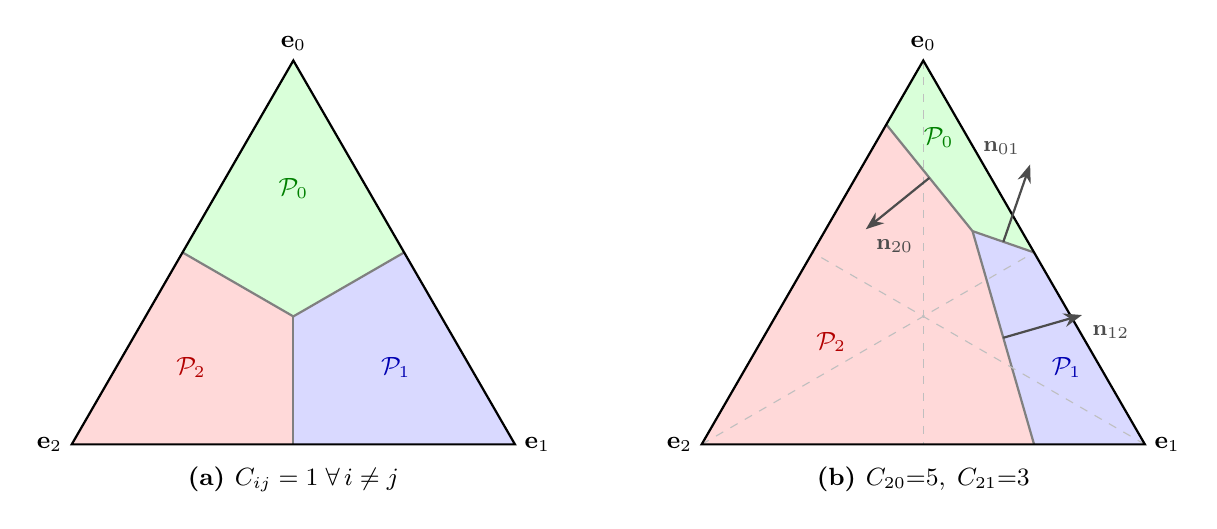
\begin{tikzpicture}[font=\sffamily]

    \begin{scope}[xshift=0.0cm, scale=0.65]
    \coordinate (Top) at (0.000, 5.000);
    \coordinate (Right) at (4.330, -2.500);
    \coordinate (Left) at (-4.330, -2.500);

    \coordinate (Int) at (0.000, 0.000);

    \fill[green!15] (0.000, 5.000) -- (2.165, 1.250) -- (0.000, 0.000) -- (-2.165, 1.250) -- cycle;
    \fill[blue!15] (4.330, -2.500) -- (0.000, -2.500) -- (0.000, 0.000) -- (2.165, 1.250) -- cycle;
    \fill[red!15] (-4.330, -2.500) -- (-2.165, 1.250) -- (0.000, 0.000) -- (0.000, -2.500) -- cycle;

    \draw[thick, black!50] (Int) -- (2.165, 1.250);
    \draw[thick, black!50] (Int) -- (-2.165, 1.250);
    \draw[thick, black!50] (Int) -- (0.000, -2.500);

    \draw[thick] (Top) -- (Right) -- (Left) -- cycle;

    \node[green!50!black, font=\small\bfseries] at (0.000, 2.500) {$\mathcal{P}_0$};
    \node[blue!70!black, font=\small\bfseries] at (2.000, -1.000) {$\mathcal{P}_1$};
    \node[red!70!black, font=\small\bfseries] at (-2.000, -1.000) {$\mathcal{P}_2$};

    \node[above, font=\small] at (Top) {$\mathbf{e}_0$};
    \node[right, font=\small] at (Right) {$\mathbf{e}_1$};
    \node[left, font=\small] at (Left) {$\mathbf{e}_2$};
    \node[font=\small\bfseries, anchor=north, align=center] at (0, -2.750) {(a) $C_{ij} = 1 \;\forall\, i \neq j$};
    \end{scope}

    \begin{scope}[xshift=8.0cm, scale=0.65]
    \coordinate (Top) at (0.000, 5.000);
    \coordinate (Right) at (4.330, -2.500);
    \coordinate (Left) at (-4.330, -2.500);

    \coordinate (Int) at (0.962, 1.667);

    \fill[green!15] (0.000, 5.000) -- (2.165, 1.250) -- (0.962, 1.667) -- (-0.722, 3.750) -- cycle;
    \fill[blue!15] (4.330, -2.500) -- (2.165, -2.500) -- (0.962, 1.667) -- (2.165, 1.250) -- cycle;
    \fill[red!15] (-4.330, -2.500) -- (-0.722, 3.750) -- (0.962, 1.667) -- (2.165, -2.500) -- cycle;

    \draw[thick, black!50] (Int) -- (2.165, 1.250);
    \draw[thick, black!50] (Int) -- (-0.722, 3.750);
    \draw[thick, black!50] (Int) -- (2.165, -2.500);

    \draw[dashed, gray!50, thin] (Left) -- (2.165, 1.250);
    \draw[dashed, gray!50, thin] (Right) -- (-2.165, 1.250);
    \draw[dashed, gray!50, thin] (Top) -- (0.000, -2.500);

    \draw[thick] (Top) -- (Right) -- (Left) -- cycle;

    % Normal vector annotations
    \coordinate (NormStart) at (1.564, 1.458);
    \draw[->, >=Stealth, thick, black!70] (NormStart) -- ++(0.524, 1.512)
        node[above left, font=\footnotesize] {$\mathbf{n}_{01}$};
    \coordinate (NormStart) at (0.120, 2.708);
    \draw[->, >=Stealth, thick, black!70] (NormStart) -- ++(-1.244, -1.006)
        node[below right, font=\footnotesize] {$\mathbf{n}_{20}$};
    \coordinate (NormStart) at (1.564, -0.417);
    \draw[->, >=Stealth, thick, black!70] (NormStart) -- ++(1.537, 0.444)
        node[below right, font=\footnotesize] {$\mathbf{n}_{12}$};

    \node[green!50!black, font=\small\bfseries] at (0.300, 3.500) {$\mathcal{P}_0$};
    \node[blue!70!black, font=\small\bfseries] at (2.800, -1.000) {$\mathcal{P}_1$};
    \node[red!70!black, font=\small\bfseries] at (-1.800, -0.500) {$\mathcal{P}_2$};

    \node[above, font=\small] at (Top) {$\mathbf{e}_0$};
    \node[right, font=\small] at (Right) {$\mathbf{e}_1$};
    \node[left, font=\small] at (Left) {$\mathbf{e}_2$};
    \node[font=\small\bfseries, anchor=north, align=center] at (0, -2.750) {(b) $C_{20}{=}5,\; C_{21}{=}3$};
    \end{scope}

\end{tikzpicture}
\end{document}
}
    \caption{Bayes-optimal decision regions on the 3-class probability simplex. \textbf{(a)}~Under symmetric 0/1 loss, boundaries are the medians meeting at the barycenter $(1/3, 1/3, 1/3)$, yielding equal-sized regions. \textbf{(b)}~Under asymmetric costs with $C_{ii}=0$, $C_{20}=5$, $C_{21}=3$, and all other off-diagonal entries equal to~1, the boundaries rotate and the intersection shifts to $(5/9, 1/3, 1/9)$, expanding $\mathcal{P}_2$ at the expense of $\mathcal{P}_0$ and $\mathcal{P}_1$. The normal vectors $\mathbf{n}_{ij} = \mathbf{c}_i - \mathbf{c}_j$ are determined entirely by the cost matrix (Theorem~\ref{thm:rigid_partition}).}\label{fig:simplex_cost_partition}
\end{figure}

The same partition admits a three-dimensional reading. Graphing each conditional-risk functional $\mathcal{L}_i(\mathbf{p}) = \mathbf{c}_i^\top \mathbf{p}$ as a plane over $\Delta^{K-1}$, the Bayes rule selects the lowest plane at each $\mathbf{p}$, and the orthogonal projection of this lower envelope onto the simplex base reproduces the 2D partition; Figure~\ref{fig:simplex_cost_partition_3d} renders both cost matrices in this view.

\begin{figure}[H]
    \centering
    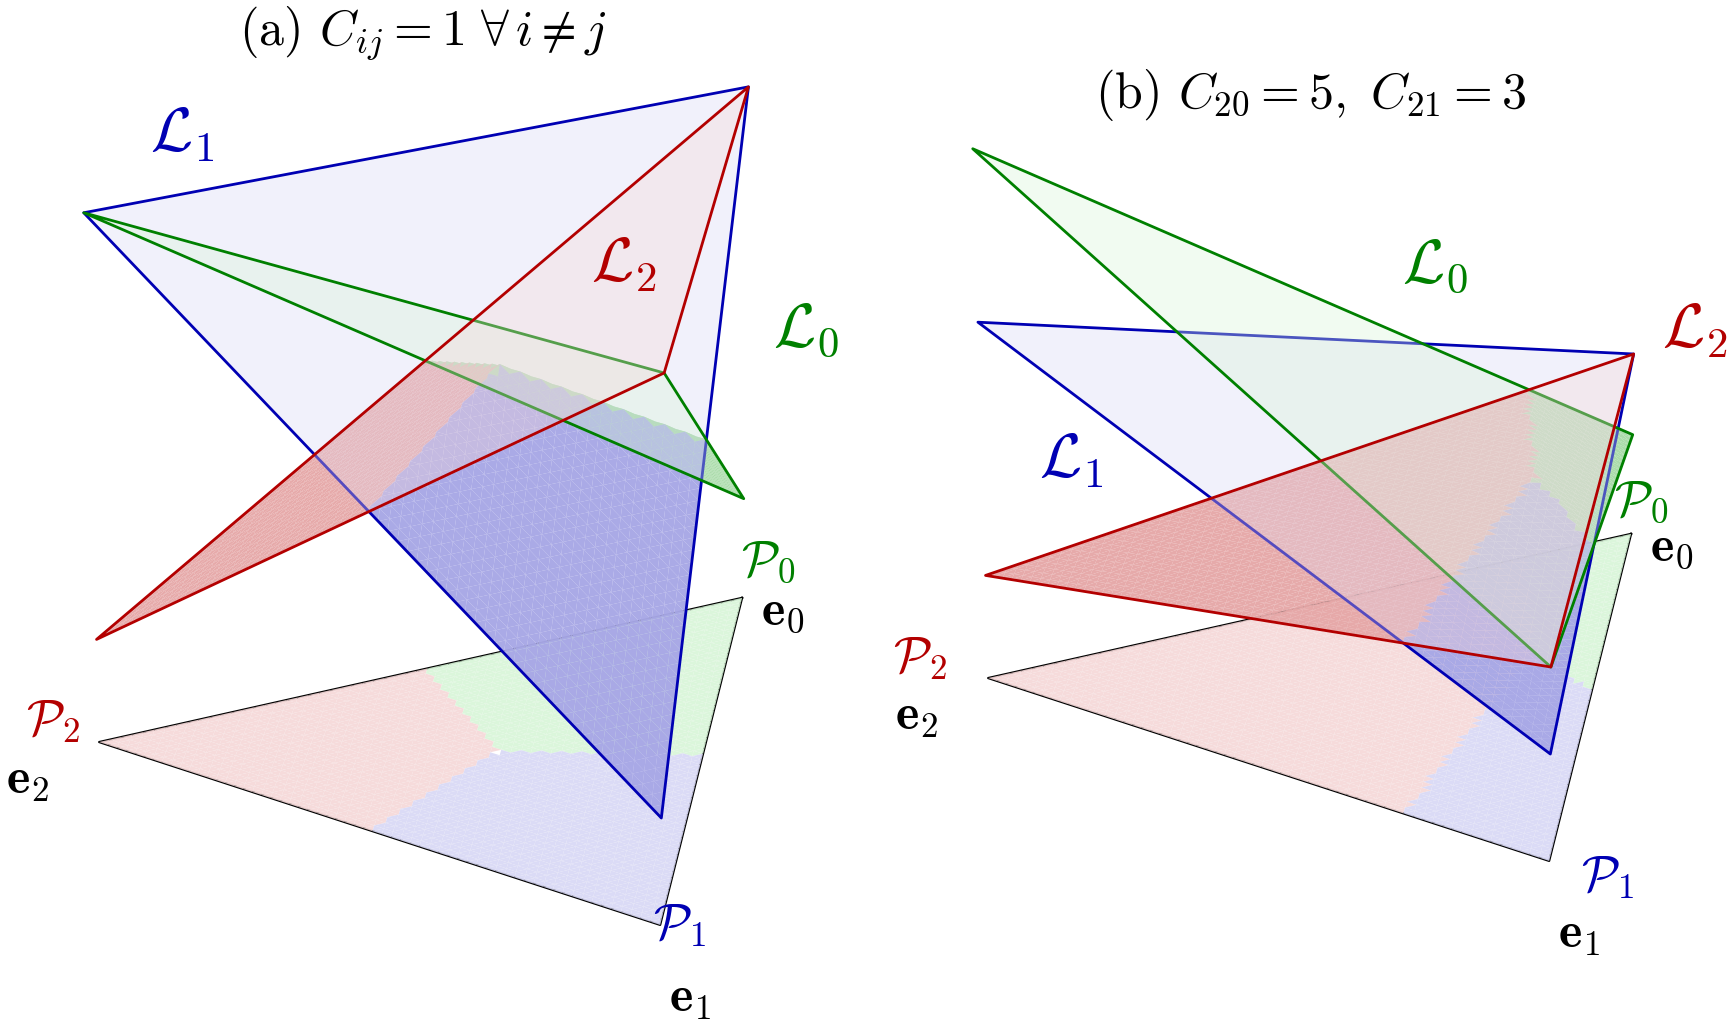
\includegraphics[width=0.72\textwidth]{figures/simplex_cost_partition_3d.png}
    \caption{Risk planes and lower envelope on the 3-class probability simplex, for the same cost matrices as Figure~\ref{fig:simplex_cost_partition}. Each semi-transparent plane graphs a conditional-risk functional $\mathcal{L}_i(\mathbf{p}) = \mathbf{c}_i^\top \mathbf{p}$ over $\Delta^2$; the opaque facets are the lower envelope $\min_i \mathcal{L}_i$, one facet per region $\mathcal{P}_i^*$ on which action $i$ is risk-minimal. Projecting the envelope vertically onto the simplex base recovers the 2D partition of Figure~\ref{fig:simplex_cost_partition}. \textbf{(a)}~Symmetric 0/1 loss yields three congruent planes meeting at the barycenter and three equal-area envelope facets. \textbf{(b)}~Under asymmetric costs $C_{20}=5,\ C_{21}=3$, plane $\mathcal{L}_2$ has steeper slopes against $\mathbf{e}_0$ and $\mathbf{e}_1$, and $\mathcal{P}_2^*$ expands at the expense of $\mathcal{P}_0^*$ and $\mathcal{P}_1^*$.}\label{fig:simplex_cost_partition_3d}
\end{figure}

\section{Limitations of the plug-in rule in the multiclass setting}\label{sec:analytical_fragility}

As in the binary case, the standard approach applies the Bayes Optimal projection (Eq.~\ref{eq:multiclass_bayes}) directly to the estimated probabilities,
\begin{equation}
    \hat{h}(x) = \underset{i \in \mathcal{Y}}{\mathrm{argmin}} \,\, \mathbf{c}_i^\top \hat{\mathbf{p}}(x).
\end{equation}
This rule attains the Bayes risk whenever, for almost every $x$, its selected action minimizes the conditional risk at the true posterior; exact posterior recovery, $\hat{\mathbf{p}}(x) = \boldsymbol{\eta}(x)$ almost everywhere, is sufficient for this but not necessary. In practice, systematic estimation errors shift the distribution of estimates within the simplex, creating a geometric mismatch between the theoretical boundaries from $\mathbf{C}$ and the effective support of the estimator.

\subsection{Systematic estimation error in the probability simplex}

Let $\Psi: \Delta^{K-1} \to \Delta^{K-1}$ denote the systematic distortion induced by the estimator, so that
$\hat{\mathbf{p}}(x) \approx \Psi(\boldsymbol{\eta}(x))$. Two common distortion regimes are especially relevant.

\paragraph{Oversmoothing.}
Strong regularization shrinks estimated probabilities toward the barycenter
$\mathbf{u} = (1/K,\ldots,1/K)^\top$. As a result, estimates may never reach the parts of the simplex where a high-penalty or minority class is Bayes-optimal. The plug-in classifier can then fail to predict that class at all, even when the estimator preserves the correct ranking among class probabilities.

\paragraph{Undersmoothing.}
At the opposite extreme, overconfident estimators push $\hat{\mathbf{p}}(x)$ toward the vertices of the simplex. If $\hat{\mathbf{p}}(x) \approx \mathbf{e}_i$, then the risk of predicting class $k$ is approximately $C_{ik}$, and the plug-in rule chooses the cheapest action in row $i$ of the cost matrix. Under element-wise reasonableness, this is simply class $i$, since $C_{ii} < C_{ik}$ for all $k \neq i$. Thus the decision reduces to the cost-blind argmax rule, and the magnitudes of the off-diagonal costs have little practical effect.

Figure~\ref{fig:simplex_distortions} illustrates these two distortions on the 3-class simplex.

\begin{figure}[H]
    \centering
    \resizebox{\textwidth}{!}{\documentclass[tikz, border=10pt]{standalone}
\usepackage{tikz}
\usepackage{amsmath}
\usetikzlibrary{calc, arrows.meta}

\begin{document}
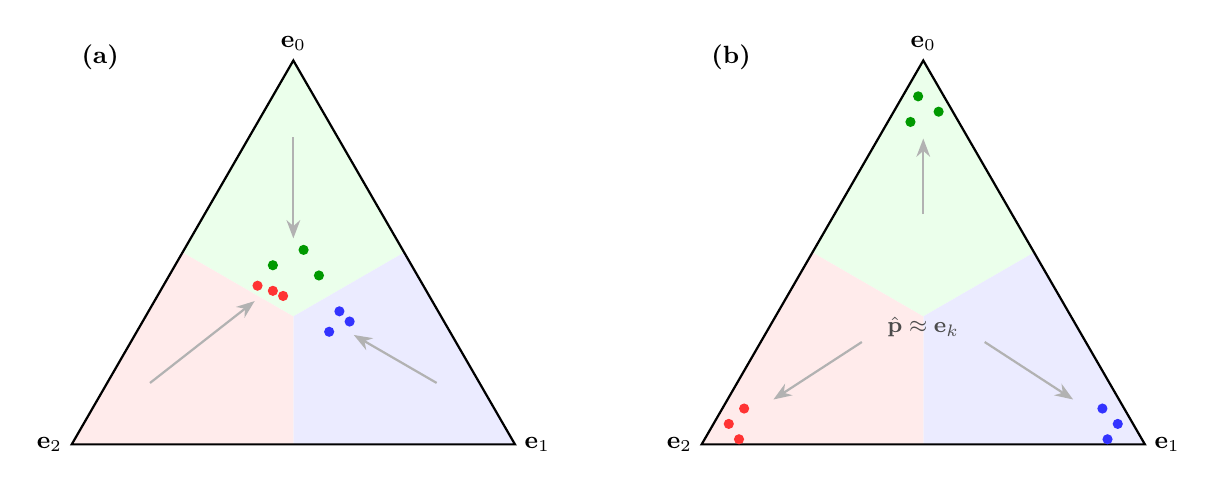
\begin{tikzpicture}[font=\sffamily]

    % ===== LEFT PANEL: Oversmoothing =====
    \begin{scope}[scale=0.65]
        % Vertices
        \coordinate (T) at (0, 5);
        \coordinate (R) at (4.33, -2.5);
        \coordinate (L) at (-4.33, -2.5);

        % Centroid and edge midpoints
        \coordinate (G) at (0, 0);
        \coordinate (MidTR) at (2.165, 1.25);
        \coordinate (MidTL) at (-2.165, 1.25);
        \coordinate (MidRL) at (0, -2.5);

        % Light region fills (same as 0/1 loss partition)
        \fill[green!8] (T) -- (MidTR) -- (G) -- (MidTL) -- cycle;
        \fill[blue!8] (R) -- (MidRL) -- (G) -- (MidTR) -- cycle;
        \fill[red!8] (L) -- (MidTL) -- (G) -- (MidRL) -- cycle;

        % Triangle frame
        \draw[thick] (T) -- (R) -- (L) -- cycle;

        % Contraction arrows (showing direction of distortion toward centroid)
        \draw[->, >=Stealth, gray!60, thick, shorten >=6pt] (0, 3.5) -- (0, 1.2);
        \draw[->, >=Stealth, gray!60, thick, shorten >=6pt] (2.8, -1.3) -- (0.9, -0.2);
        \draw[->, >=Stealth, gray!60, thick, shorten >=6pt] (-2.8, -1.3) -- (-0.5, 0.5);

        % Estimated points colored by TRUE class, all clustered near centroid
        % Class 0 (green) — estimates still in R_0
        \node[circle, fill=green!60!black, inner sep=1.3pt] at (0.2, 1.3) {};
        \node[circle, fill=green!60!black, inner sep=1.3pt] at (-0.4, 1.0) {};
        \node[circle, fill=green!60!black, inner sep=1.3pt] at (0.5, 0.8) {};

        % Class 1 (blue) — estimates still in R_1
        \node[circle, fill=blue!80, inner sep=1.3pt] at (0.9, 0.1) {};
        \node[circle, fill=blue!80, inner sep=1.3pt] at (0.7, -0.3) {};
        \node[circle, fill=blue!80, inner sep=1.3pt] at (1.1, -0.1) {};

        % Class 2 (red) — estimates in R_0, NOT in R_2 (misclassified)
        \node[circle, fill=red!80, inner sep=1.3pt] at (-0.4, 0.5) {};
        \node[circle, fill=red!80, inner sep=1.3pt] at (-0.2, 0.4) {};
        \node[circle, fill=red!80, inner sep=1.3pt] at (-0.7, 0.6) {};

        % Vertex labels
        \node[above, font=\small] at (T) {$\mathbf{e}_0$};
        \node[right, font=\small] at (R) {$\mathbf{e}_1$};
        \node[left, font=\small] at (L) {$\mathbf{e}_2$};

        % Panel label
        \node[font=\small\bfseries, anchor=north west] at (-4.33, 5.5) {(a)};
    \end{scope}

    % ===== RIGHT PANEL: Undersmoothing =====
    \begin{scope}[xshift=8cm, scale=0.65]
        % Vertices
        \coordinate (T) at (0, 5);
        \coordinate (R) at (4.33, -2.5);
        \coordinate (L) at (-4.33, -2.5);

        % Centroid and edge midpoints
        \coordinate (G) at (0, 0);
        \coordinate (MidTR) at (2.165, 1.25);
        \coordinate (MidTL) at (-2.165, 1.25);
        \coordinate (MidRL) at (0, -2.5);

        % Light region fills
        \fill[green!8] (T) -- (MidTR) -- (G) -- (MidTL) -- cycle;
        \fill[blue!8] (R) -- (MidRL) -- (G) -- (MidTR) -- cycle;
        \fill[red!8] (L) -- (MidTL) -- (G) -- (MidRL) -- cycle;

        % Triangle frame
        \draw[thick] (T) -- (R) -- (L) -- cycle;

        % Expansion arrows (showing direction of distortion toward vertices)
        \draw[->, >=Stealth, gray!60, thick, shorten >=6pt] (0, 2.0) -- (0, 3.8);
        \draw[->, >=Stealth, gray!60, thick, shorten >=6pt] (1.2, -0.5) -- (3.2, -1.8);
        \draw[->, >=Stealth, gray!60, thick, shorten >=6pt] (-1.2, -0.5) -- (-3.2, -1.8);

        % Data points clustered near vertices (overconfident)
        % Class 0 near Top
        \node[circle, fill=green!60!black, inner sep=1.3pt] at (-0.1, 4.3) {};
        \node[circle, fill=green!60!black, inner sep=1.3pt] at (0.3, 4.0) {};
        \node[circle, fill=green!60!black, inner sep=1.3pt] at (-0.25, 3.8) {};

        % Class 1 near Right
        \node[circle, fill=blue!80, inner sep=1.3pt] at (3.8, -2.1) {};
        \node[circle, fill=blue!80, inner sep=1.3pt] at (3.5, -1.8) {};
        \node[circle, fill=blue!80, inner sep=1.3pt] at (3.6, -2.4) {};

        % Class 2 near Left
        \node[circle, fill=red!80, inner sep=1.3pt] at (-3.8, -2.1) {};
        \node[circle, fill=red!80, inner sep=1.3pt] at (-3.5, -1.8) {};
        \node[circle, fill=red!80, inner sep=1.3pt] at (-3.6, -2.4) {};

        % Annotation
        \node[black!70, font=\footnotesize, align=center] at (0, -0.2)
            {$\hat{\mathbf{p}} \approx \mathbf{e}_k$};

        % Vertex labels
        \node[above, font=\small] at (T) {$\mathbf{e}_0$};
        \node[right, font=\small] at (R) {$\mathbf{e}_1$};
        \node[left, font=\small] at (L) {$\mathbf{e}_2$};

        % Panel label
        \node[font=\small\bfseries, anchor=north west] at (-4.33, 5.5) {(b)};
    \end{scope}

\end{tikzpicture}
\end{document}
}
    \caption{Effects of estimation error on the 3-class simplex. \textbf{(a)}~Probability contraction (oversmoothing) shrinks the estimator's image $\mathrm{Im}(\Psi)$ into a sub-region $\mathcal{S}$ near the barycenter. If $\mathcal{S}$ does not intersect $\mathcal{P}_2^*$, the classifier has zero recall for class~2 even though the decision boundary is correct. \textbf{(b)}~Overconfidence (undersmoothing) pushes estimates toward vertices ($\hat{\mathbf{p}} \approx \mathbf{e}_k$), making all points fall deep inside their respective argmax regions. The cost structure becomes irrelevant since $\mathrm{argmin}_{k \in \mathcal{Y}} \mathbf{c}_k^\top \hat{\mathbf{p}}$ reduces to $\mathrm{argmax}_{k \in \mathcal{Y}} \hat{p}_k$.}\label{fig:simplex_distortions}
\end{figure}

\subsection{The inverse-map problem}

Even when $\Psi$ is a bijection on $\Delta^{K-1}$ and the discriminative ranking is preserved, the analytical rule applied in the estimate space is not Bayes-optimal. The analytical boundary lives in the true-probability space, $\mathcal{B}_{ij} = \{\mathbf{p} \in \mathbb{R}^K \mid (\mathbf{c}_i - \mathbf{c}_j)^\top \mathbf{p} = 0\}$, so the corresponding boundary in the estimate space is its pre-image
\begin{equation}
    \tilde{\mathcal{B}}_{ij} = \Psi^{-1}(\mathcal{B}_{ij}) = \{ \mathbf{z} \in \Delta^{K-1} \mid (\mathbf{c}_i - \mathbf{c}_j)^\top \Psi^{-1}(\mathbf{z}) = 0 \}.
\end{equation}
Because $\Psi$ is generically non-linear, $\tilde{\mathcal{B}}_{ij}$ is a curved manifold, not a hyperplane. Applying the analytical rule with the fixed normals $\mathbf{n}_{ij} = \mathbf{c}_i - \mathbf{c}_j$ in estimate space therefore introduces an approximation error that translation alone cannot eliminate. Two corrective routes follow: estimate $\Psi^{-1}$ with a low-parameter family before applying the analytical rule (post-hoc calibration, Section~\ref{sec:multiclass_calibration}), or skip the inverse map entirely and learn a new partition of the estimate simplex directly (Chapter~\ref{sec:partition_optimization}).

\section{Post-hoc calibration in the multiclass setting}\label{sec:multiclass_calibration}

Multiclass perfect calibration requires $\mathbb{P}(Y{=}k \mid \hat{\mathbf{p}}(X) = \mathbf{q}) = q_k$ for all $k$ and almost every $\mathbf{q} \in \Delta^{K-1}$ under the law of $\hat{\mathbf{p}}(X)$, a joint condition over the simplex strictly stronger than the per-class binary condition (Definition~\ref{def:calibration}). The calibrators that extend the binary methods to $K > 2$ trade off in how much of this joint structure they attempt to model.

\paragraph{Temperature scaling.} The most conservative extension \citep{guo2017calibration} applies a single scalar $T > 0$ to the logit vector before the softmax: $g_T(\hat{\mathbf{p}}) = \mathrm{softmax}(\mathbf{z}/T)$ with $z_k = \log \hat{p}_k$. Like its binary analogue, it preserves the ranking of all $K$ classes and has only one degree of freedom, so it is the most data-efficient option but cannot redistribute mass between classes asymmetrically.

\paragraph{Platt scaling.} Extends temperature scaling by a one-vs-rest decomposition: each class $k$ receives its own two-parameter sigmoid calibrator fitted on the binary task ``class $k$ vs.\ rest'', and the $K$ outputs are renormalized to sum to one. The total parameter count is $2K$, so the family can correct class-specific overconfidence but ignores cross-class interactions: the calibrator for class $k$ is blind to the joint shape of the score distribution over the other $K-1$ classes.

\paragraph{Isotonic regression.} Applies the same one-vs-rest decomposition with non-parametric monotone calibrators in place of the sigmoid; its complexity is adaptive in the calibration-set size rather than fixed in $K$, and it inherits the same cross-class blindness.

\paragraph{Dirichlet calibration.} Natively multiclass \citep{kull2019beyond}, this calibrator models exactly those cross-class interactions. The full parameterization
\[
g_{\mathbf{W},\mathbf{b}}(\hat{\mathbf{p}}) = \mathrm{softmax}(\mathbf{W} \log \hat{\mathbf{p}} + \mathbf{b}),
\quad \mathbf{W} \in \mathbb{R}^{K \times K},\; \mathbf{b} \in \mathbb{R}^K
\]
(Eq.~\ref{eq:dirichlet_calibration}) acts as a log-linear transformation on the simplex with $K^2 + K$ free parameters. Setting $\mathbf{W} = (1/T)\,\mathbf{I}$ with $\mathbf{b} = \mathbf{0}$ recovers temperature scaling, and the full $\mathbf{W}$ is the maximally expressive log-linear case; intermediate restrictions on $\mathbf{W}$ correspond to the vector and matrix scaling variants of \citet{guo2017calibration}.

The parametric calibrators can be ordered by flexibility. Temperature scaling uses a single parameter and preserves the class ranking, so it can correct global overconfidence but not class-specific distortions. One-vs-rest Platt scaling introduces $2K$ parameters and can correct per-class miscalibration, but because each class is calibrated against the rest independently, it does not model cross-class interactions. Dirichlet calibration is the most expressive of the three: with $K^2+K$ parameters, it applies a log-linear transformation to the full probability vector and can represent interactions among classes. Isotonic regression occupies a separate position in the comparison, since its non-parametric monotone complexity depends on the calibration-set size rather than on a fixed parameter count in $K$.

Each calibrator can be composed with either the cost-blind argmax rule or the analytical cost-sensitive rule in Eq.~\ref{eq:multiclass_bayes}, yielding a \textit{calibrate-then-decide} strategy. As in the binary case, the argument of Proposition~\ref{prop:calibrate_then_decide} extends: recovering the true posterior vector, $g(\hat{\mathbf{p}}(x)) = \boldsymbol{\eta}(x)$ almost everywhere, makes the analytical rule applied to $g(\hat{\mathbf{p}}(x))$ attain the Bayes risk. Perfect multiclass calibration alone does not imply this posterior-recovery condition. In practice, calibration is only approximate, and the remaining distortion motivates the direct partition-optimization strategies of Chapter~\ref{sec:partition_optimization}.

%!TeX root=../carlo_master.tex
\chapter{Approaches to partition optimization}\label{sec:partition_optimization}

A line of work going back to \citet{obrien2008costsensitive} replaces the fixed analytical baseline with a learnable decision rule that minimizes empirical risk on a validation set, rather than relying on the theoretical partition derived from a potentially miscalibrated estimator. This chapter compares five parameterizations of that learnable rule: parallel shift on the cost matrix, linear scaling, probability-ratio thresholding, the multidimensional-thresholding view of \citet{legnaro2025multiclass}, and a priority-based sequential cascade. The first four induce convex-polytope partitions and are compared by which boundary normals each can express; they cluster into a hierarchy. Its top tier, $\mathcal{H}_{Full}$ (Section~\ref{sec:partition_matrix_framework}, Eq.~\ref{eq:hfull_def}), is the class of decision rules $\delta_{\mathbf{A}}(\mathbf{p}) = \underset{i \in \mathcal{Y}}{\mathrm{argmin}} \, \mathbf{a}_i^\top \mathbf{p}$ induced by an unconstrained learnable partition matrix $\mathbf{A} \in \mathbb{R}^{K \times K}$; its middle tier, $\mathcal{H}_{PS}$ (Eq.~\ref{eq:hps_def}), is the parallel-shift subclass that fixes the boundary normals at the cost-matrix differences but cannot rotate them. We collectively refer to the three classes $\mathcal{H}_{PS}$, $\mathcal{H}_{Sc}$, $\mathcal{H}_{Full}$, all parameterized through the partition matrix $\mathbf{A}$ of Section~\ref{sec:partition_matrix_framework}, as the \emph{matrix-parameterized methods}, and to the $K{-}1$-parameter subset $\mathcal{H}_{PS} \cup \mathcal{H}_{Sc}$, in which a single $K$-vector translates or rescales the cost-matrix columns, as the \emph{vector-tuned methods}. Their sample complexity is analysed together in Chapter~\ref{sec:voronoi_tessellation}. The sequential cascade sits outside this hierarchy: its decision regions are non-convex and order-dependent, and we include it as a heuristic contrast to the polytope methods.

\section{The partition matrix framework}\label{sec:partition_matrix_framework}

\citet{obrien2008costsensitive} formalized the problem of learning the decision rule from validation data as \textit{partition learning}: decouple the \textit{evaluation cost matrix} $\mathbf{C}$, which defines the ground-truth penalty, from the \textit{decision partition matrix} $\mathbf{A}$, which parameterizes the decision boundary.

Let $\mathbf{A} \in \mathbb{R}^{K \times K}$ be a learnable parameter matrix. The decision rule is defined as minimizing the ``apparent'' risk parameterized by $\mathbf{A}$,
\begin{equation}\label{eq:obrien_rule}
    \delta_{\mathbf{A}}(\mathbf{p}) = \underset{i \in \mathcal{Y}}{\mathrm{argmin}} \sum_{j=0}^{K-1} A_{ji} p_j = \underset{i \in \mathcal{Y}}{\mathrm{argmin}} \,\, \mathbf{a}_i^\top \mathbf{p},
\end{equation}
where $\mathbf{a}_i$ denotes the $i$-th column of $\mathbf{A}$ (the apparent costs of predicting class $i$ across all possible truth labels).
The optimization objective is to find the matrix $\mathbf{A}^*$ that minimizes the \textit{true} empirical risk, evaluated using $\mathbf{C}$ on the plug-in classifier $\delta_{\mathbf{A}} \circ \hat{\mathbf{p}}$, over the validation set $\mathcal{V}$,
\begin{equation}
    \mathbf{A}^* = \underset{\mathbf{A} \in \mathbb{R}^{K \times K}}{\mathrm{argmin}} \sum_{(x, y) \in \mathcal{V}} C_{y, \,\delta_{\mathbf{A}}(\hat{\mathbf{p}}(x))}.
\end{equation}
Choosing $\mathbf{A}^*$ by minimizing this empirical risk over $\mathcal{V}$ is the multiclass instance of the decision-stage learning problem (Section~\ref{sec:decision_learning}): empirical risk minimization over $\mathcal{H}_{dec}$, here parameterized by the partition matrix $\mathbf{A}$.
Learning all $K^2$ entries of $\mathbf{A}$ is prone to overfitting, which is why \citet{obrien2008costsensitive} proposed structural constraints on $\mathbf{A}$ corresponding to specific geometric transformations of the boundaries.

The admissibility and element-wise reasonableness conditions (Definitions~\ref{def:admissibility} and~\ref{def:elementwise}) constrain only the evaluation matrix $\mathbf{C}$. We place no such restriction on the decision matrix $\mathbf{A}$: the unconstrained partition class is
\begin{equation}\label{eq:hfull_def}
    \mathcal{H}_{Full} = \left\{ \delta(\mathbf{p}) = \underset{k \in \mathcal{Y}}{\mathrm{argmin}} \,\, \mathbf{a}_k^\top \mathbf{p} \mid \mathbf{A} \in \mathbb{R}^{K \times K} \right\},
\end{equation}
with $\mathbf{a}_k$ ranging over all of $\mathbb{R}^{K}$.

\section{Geometric regularization strategies}

The four constraints below sit on a spectrum of how aggressively they reduce $\mathcal{H}_{Full}$. All can be fit by empirical optimization on a validation set, so the learning objective need not be tied to a specified cost matrix: the same search can target cost-sensitive risk, macro $F_1$, macro G-Mean, or any other task utility. What distinguishes the methods below is not the optimization criterion but the geometry of the partitions they can express.

The first two (parallel shift and linear scaling) come from \citet{obrien2008costsensitive}; the third is the per-class probability rescaling of \citet{lachiche2003improving}, recast here in cost-agnostic form; the fourth, due to \citet{legnaro2025multiclass}, parameterizes the decision rule directly on the simplex and, as we show below, is mathematically equivalent to the parallel shift under $0/1$ loss.

\subsection{Parallel shift parameterization}\label{sec:parallel_shifts}

The strongest strategy identified by \citet{obrien2008costsensitive} constrains $\mathbf{A}$ to be a column-wise translation of $\mathbf{C}$, one bias per predicted class. Introducing a learnable bias vector $\boldsymbol{\alpha} \in \mathbb{R}^K$,
\begin{equation}
    A_{ij} = C_{ij} + \alpha_j.
\end{equation}
This formulation has $K-1$ degrees of freedom (since shifting all $\alpha_j$ by a constant does not change the argmin).

\begin{proposition}[Parallel boundary invariance]\label{prop:parallel_invariance}
    Let $\mathcal{B}_{ij}(\mathbf{C})$ be the theoretical decision boundary between class $i$ and $j$ induced by $\mathbf{C}$. The boundary $\mathcal{B}_{ij}(\mathbf{A})$ induced by the parallel shift parameterization is parallel to $\mathcal{B}_{ij}(\mathbf{C})$.
\end{proposition}

\begin{proof}
    The boundary between class $i$ and $j$ is the locus of points where the apparent risks are equal,
    \begin{align}
        \sum_{k=0}^{K-1} (C_{ki} + \alpha_i) p_k &= \sum_{k=0}^{K-1} (C_{kj} + \alpha_j) p_k \\
        \mathbf{c}_i^\top \mathbf{p} + \alpha_i \underbrace{\sum_{k=0}^{K-1} p_k}_{1} &= \mathbf{c}_j^\top \mathbf{p} + \alpha_j \underbrace{\sum_{k=0}^{K-1} p_k}_{1} \\
        (\mathbf{c}_i - \mathbf{c}_j)^\top \mathbf{p} + (\alpha_i - \alpha_j) &= 0.
    \end{align}
    The normal vector of this hyperplane remains $\mathbf{n}_{ij} = \mathbf{c}_i - \mathbf{c}_j$, identical to the theoretical boundary. The term $(\alpha_i - \alpha_j)$ acts as a scalar offset, translating the hyperplane along the normal vector.
\end{proof}

The parallel-shift constraint corrects monotonic calibration bias (global over- or undersmoothing in the sense of Section~\ref{sec:analytical_fragility}) without changing the cost-aware orientation of any boundary. When $\hat{\mathbf{p}}$ systematically underestimates a minority class $i$, the optimizer can lower $\alpha_i$ relative to the other classes to enlarge $\mathcal{P}_i^{\boldsymbol{\alpha}}$, leaving the relative trade-off between the remaining classes unchanged. Figure~\ref{fig:obrien_parallel_shifts} illustrates this on an asymmetric cost matrix: a lowered bias entry enlarges its region by translating the bordering boundaries while keeping every boundary normal fixed.

\begin{figure}[H]
    \centering
    \resizebox{\textwidth}{!}{\documentclass[tikz, border=10pt]{standalone}
\usepackage{tikz}
\usepackage{amsmath}
\usetikzlibrary{shapes, calc, backgrounds, arrows.meta}

\begin{document}
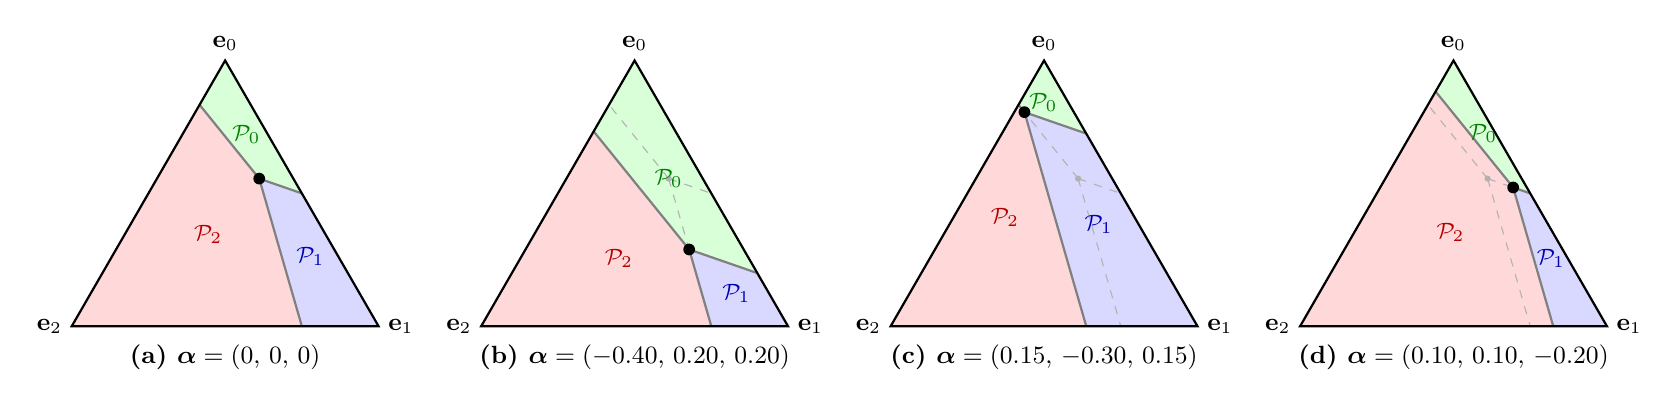
\begin{tikzpicture}[font=\sffamily]

    \begin{scope}[xshift=0.0cm, scale=0.45]
    \coordinate (Top) at (0.000, 5.000);
    \coordinate (Right) at (4.330, -2.500);
    \coordinate (Left) at (-4.330, -2.500);

    \coordinate (Int) at (0.962, 1.667);

    \fill[green!15] (0.000, 5.000) -- (2.165, 1.250) -- (0.962, 1.667) -- (-0.722, 3.750) -- cycle;
    \fill[blue!15] (4.330, -2.500) -- (2.165, -2.500) -- (0.962, 1.667) -- (2.165, 1.250) -- cycle;
    \fill[red!15] (-4.330, -2.500) -- (-0.722, 3.750) -- (0.962, 1.667) -- (2.165, -2.500) -- cycle;

    \draw[thick, black!50] (Int) -- (2.165, 1.250);
    \draw[thick, black!50] (Int) -- (-0.722, 3.750);
    \draw[thick, black!50] (Int) -- (2.165, -2.500);

    \draw[thick] (Top) -- (Right) -- (Left) -- cycle;

    \node[circle, fill=black, inner sep=1.5pt] at (Int) {};

    \node[green!50!black, font=\footnotesize\bfseries] at (0.601, 2.917) {$\mathcal{P}_0$};
    \node[blue!70!black, font=\footnotesize\bfseries] at (2.406, -0.521) {$\mathcal{P}_1$};
    \node[red!70!black, font=\footnotesize\bfseries] at (-0.481, 0.104) {$\mathcal{P}_2$};

    \node[above, font=\small] at (Top) {$\mathbf{e}_0$};
    \node[right, font=\small] at (Right) {$\mathbf{e}_1$};
    \node[left, font=\small] at (Left) {$\mathbf{e}_2$};
    \node[font=\small\bfseries, anchor=north, align=center] at (0, -2.750) {(a) $\boldsymbol{\alpha} = (0,\,0,\,0)$};
    \end{scope}

    \begin{scope}[xshift=5.2cm, scale=0.45]
    \coordinate (Top) at (0.000, 5.000);
    \coordinate (Right) at (4.330, -2.500);
    \coordinate (Left) at (-4.330, -2.500);

    \coordinate (Int) at (1.540, -0.333);

    \fill[green!15] (0.000, 5.000) -- (3.464, -1.000) -- (1.540, -0.333) -- (-1.155, 3.000) -- cycle;
    \fill[blue!15] (4.330, -2.500) -- (2.165, -2.500) -- (1.540, -0.333) -- (3.464, -1.000) -- cycle;
    \fill[red!15] (-4.330, -2.500) -- (-1.155, 3.000) -- (1.540, -0.333) -- (2.165, -2.500) -- cycle;

    \coordinate (OvInt) at (0.962, 1.667);
    \draw[dashed, gray!60, thin] (OvInt) -- (2.165, 1.250);
    \draw[dashed, gray!60, thin] (OvInt) -- (-0.722, 3.750);
    \draw[dashed, gray!60, thin] (OvInt) -- (2.165, -2.500);
    \node[circle, fill=gray!60, inner sep=0.8pt] at (OvInt) {};

    \draw[thick, black!50] (Int) -- (3.464, -1.000);
    \draw[thick, black!50] (Int) -- (-1.155, 3.000);
    \draw[thick, black!50] (Int) -- (2.165, -2.500);

    \draw[thick] (Top) -- (Right) -- (Left) -- cycle;

    \node[circle, fill=black, inner sep=1.5pt] at (Int) {};

    \node[green!50!black, font=\footnotesize\bfseries] at (0.962, 1.667) {$\mathcal{P}_0$};
    \node[blue!70!black, font=\footnotesize\bfseries] at (2.875, -1.583) {$\mathcal{P}_1$};
    \node[red!70!black, font=\footnotesize\bfseries] at (-0.445, -0.583) {$\mathcal{P}_2$};

    \node[above, font=\small] at (Top) {$\mathbf{e}_0$};
    \node[right, font=\small] at (Right) {$\mathbf{e}_1$};
    \node[left, font=\small] at (Left) {$\mathbf{e}_2$};
    \node[font=\small\bfseries, anchor=north, align=center] at (0, -2.750) {(b) $\boldsymbol{\alpha} = (-0.40,\,0.20,\,0.20)$};
    \end{scope}

    \begin{scope}[xshift=10.4cm, scale=0.45]
    \coordinate (Top) at (0.000, 5.000);
    \coordinate (Right) at (4.330, -2.500);
    \coordinate (Left) at (-4.330, -2.500);

    \coordinate (Int) at (-0.553, 3.542);

    \fill[green!15] (0.000, 5.000) -- (1.191, 2.938) -- (-0.553, 3.542) -- (-0.722, 3.750) -- cycle;
    \fill[blue!15] (4.330, -2.500) -- (1.191, -2.500) -- (-0.553, 3.542) -- (1.191, 2.938) -- cycle;
    \fill[red!15] (-4.330, -2.500) -- (-0.722, 3.750) -- (-0.553, 3.542) -- (1.191, -2.500) -- cycle;

    \coordinate (OvInt) at (0.962, 1.667);
    \draw[dashed, gray!60, thin] (OvInt) -- (2.165, 1.250);
    \draw[dashed, gray!60, thin] (OvInt) -- (-0.722, 3.750);
    \draw[dashed, gray!60, thin] (OvInt) -- (2.165, -2.500);
    \node[circle, fill=gray!60, inner sep=0.8pt] at (OvInt) {};

    \draw[thick, black!50] (Int) -- (1.191, 2.938);
    \draw[thick, black!50] (Int) -- (-0.722, 3.750);
    \draw[thick, black!50] (Int) -- (1.191, -2.500);

    \draw[thick] (Top) -- (Right) -- (Left) -- cycle;

    \node[circle, fill=black, inner sep=1.5pt] at (Int) {};

    \node[green!50!black, font=\footnotesize\bfseries] at (-0.021, 3.807) {$\mathcal{P}_0$};
    \node[blue!70!black, font=\footnotesize\bfseries] at (1.540, 0.370) {$\mathcal{P}_1$};
    \node[red!70!black, font=\footnotesize\bfseries] at (-1.104, 0.573) {$\mathcal{P}_2$};

    \node[above, font=\small] at (Top) {$\mathbf{e}_0$};
    \node[right, font=\small] at (Right) {$\mathbf{e}_1$};
    \node[left, font=\small] at (Left) {$\mathbf{e}_2$};
    \node[font=\small\bfseries, anchor=north, align=center] at (0, -2.750) {(c) $\boldsymbol{\alpha} = (0.15,\,-0.30,\,0.15)$};
    \end{scope}

    \begin{scope}[xshift=15.600000000000001cm, scale=0.45]
    \coordinate (Top) at (0.000, 5.000);
    \coordinate (Right) at (4.330, -2.500);
    \coordinate (Left) at (-4.330, -2.500);

    \coordinate (Int) at (1.684, 1.417);

    \fill[green!15] (0.000, 5.000) -- (2.165, 1.250) -- (1.684, 1.417) -- (-0.505, 4.125) -- cycle;
    \fill[blue!15] (4.330, -2.500) -- (2.815, -2.500) -- (1.684, 1.417) -- (2.165, 1.250) -- cycle;
    \fill[red!15] (-4.330, -2.500) -- (-0.505, 4.125) -- (1.684, 1.417) -- (2.815, -2.500) -- cycle;

    \coordinate (OvInt) at (0.962, 1.667);
    \draw[dashed, gray!60, thin] (OvInt) -- (2.165, 1.250);
    \draw[dashed, gray!60, thin] (OvInt) -- (-0.722, 3.750);
    \draw[dashed, gray!60, thin] (OvInt) -- (2.165, -2.500);
    \node[circle, fill=gray!60, inner sep=0.8pt] at (OvInt) {};

    \draw[thick, black!50] (Int) -- (2.165, 1.250);
    \draw[thick, black!50] (Int) -- (-0.505, 4.125);
    \draw[thick, black!50] (Int) -- (2.815, -2.500);

    \draw[thick] (Top) -- (Right) -- (Left) -- cycle;

    \node[circle, fill=black, inner sep=1.5pt] at (Int) {};

    \node[green!50!black, font=\footnotesize\bfseries] at (0.836, 2.948) {$\mathcal{P}_0$};
    \node[blue!70!black, font=\footnotesize\bfseries] at (2.748, -0.583) {$\mathcal{P}_1$};
    \node[red!70!black, font=\footnotesize\bfseries] at (-0.084, 0.135) {$\mathcal{P}_2$};

    \node[above, font=\small] at (Top) {$\mathbf{e}_0$};
    \node[right, font=\small] at (Right) {$\mathbf{e}_1$};
    \node[left, font=\small] at (Left) {$\mathbf{e}_2$};
    \node[font=\small\bfseries, anchor=north, align=center] at (0, -2.750) {(d) $\boldsymbol{\alpha} = (0.10,\,0.10,\,-0.20)$};
    \end{scope}

\end{tikzpicture}
\end{document}
}
    \caption{O'Brien's parallel-shift regularization on the asymmetric cost matrix $\mathbf{C}$ with $C_{20}=5$, $C_{21}=3$ (same as panel~(b) of Figure~\ref{fig:simplex_cost_partition}). Panel~(a) shows the baseline $\mathbf{A}=\mathbf{C}$. Panels~(b)--(d) show $\mathbf{A}=\mathbf{C}+\mathbf{1}\boldsymbol{\alpha}^\top$ for three choices of the bias vector $\boldsymbol{\alpha}$, with dashed gray segments reproducing panel~(a)'s boundaries for reference. In each panel one entry of $\boldsymbol{\alpha}$ is set below the other two equal entries. Since $\mathcal{B}_{ij}$ depends only on $\alpha_i-\alpha_j$, the two boundaries bordering the favored class $i$ translate parallel to themselves and enlarge $\mathcal{P}_i^{\boldsymbol{\alpha}}$, while the boundary between the two equal-bias classes stays fixed (Proposition~\ref{prop:parallel_invariance}).}\label{fig:obrien_parallel_shifts}
\end{figure}

\subsection{Linear class scaling}\label{sec:linear_scaling}

An alternative parameterization scales each truth class by a learnable weight (a row-wise scaling under our convention; this corresponds to the column-wise scaling of \citet{obrien2008costsensitive}, who index $\mathbf{C}$ with the transposed convention). Let $\boldsymbol{\beta} \in \mathbb{R}^K_{\ge 0}$ be a vector of scaling factors, such that
\begin{equation}
    A_{ij} = C_{ij} \beta_i.
\end{equation}
This transformation is equivalent to modifying the estimated probabilities themselves, effectively replacing $\hat{p}_j(x)$ with a reweighted $\hat{p}'_j(x) \propto \beta_j \hat{p}_j(x)$.

\begin{proposition}[Boundary rotation under linear scaling]\label{prop:column_rotation}
    Unlike parallel shifts, linear scaling rotates the decision boundaries. Specifically, the boundary between classes $i$ and $j$ under linear scaling has normal vector $\mathbf{n}_{ij}^{(\boldsymbol{\beta})} = [(C_{0i} - C_{0j})\beta_0, \ldots, (C_{K-1,i} - C_{K-1,j})\beta_{K-1}]^\top$, which is in general not proportional to the unscaled normal $\mathbf{c}_i - \mathbf{c}_j$.
\end{proposition}

\begin{proof}
Under linear scaling, the decision boundary between classes $i$ and $j$ is the locus where their modified risks are equal,
\begin{equation}
    \sum_{k=0}^{K-1} C_{ki} \beta_k p_k = \sum_{k=0}^{K-1} C_{kj} \beta_k p_k.
\end{equation}
Rearranging yields $\sum_{k=0}^{K-1} (C_{ki} - C_{kj}) \beta_k p_k = 0$, which defines a hyperplane with normal vector
\begin{equation}
    \mathbf{n}_{ij}^{(\boldsymbol{\beta})} = \left[(C_{0i} - C_{0j})\beta_0, \; \ldots, \; (C_{K-1,i} - C_{K-1,j})\beta_{K-1}\right]^\top.
\end{equation}
In contrast, the unscaled normal is $\mathbf{n}_{ij} = \mathbf{c}_i - \mathbf{c}_j$, with components $(C_{ki} - C_{kj})$. The scaled normal $\mathbf{n}_{ij}^{(\boldsymbol{\beta})}$ is obtained by component-wise multiplication with $\boldsymbol{\beta}$, so $\mathbf{n}_{ij}^{(\boldsymbol{\beta})} = \boldsymbol{\beta} \odot \mathbf{n}_{ij}$, where $\odot$ denotes the Hadamard (element-wise) product. If $\boldsymbol{\beta}$ is not proportional to $\mathbf{1}$ and $\mathbf{n}_{ij}$ has at least two nonzero components with distinct $\beta$ values, then $\mathbf{n}_{ij}^{(\boldsymbol{\beta})} \not\propto \mathbf{n}_{ij}$, confirming that the boundary has rotated.
\end{proof}

Linear scaling is closely related to the per-class probability weighting of \citet{lachiche2003improving}, who learn one multiplicative weight per class for the estimated probabilities by greedy hill-climbing. Geometrically, this is the same kind of operation described above: it changes the boundary normals by reweighting the coordinates of the probability simplex.

Figure~\ref{fig:obrien_vs_column_scaling} contrasts the linear scaling with the parallel-shift parameterizations on a shared asymmetric cost matrix.

\begin{figure}[H]
    \centering
    \resizebox{\textwidth}{!}{\documentclass[tikz, border=10pt]{standalone}
\usepackage{tikz}
\usepackage{amsmath}
\usetikzlibrary{shapes, calc, backgrounds, arrows.meta}

\begin{document}
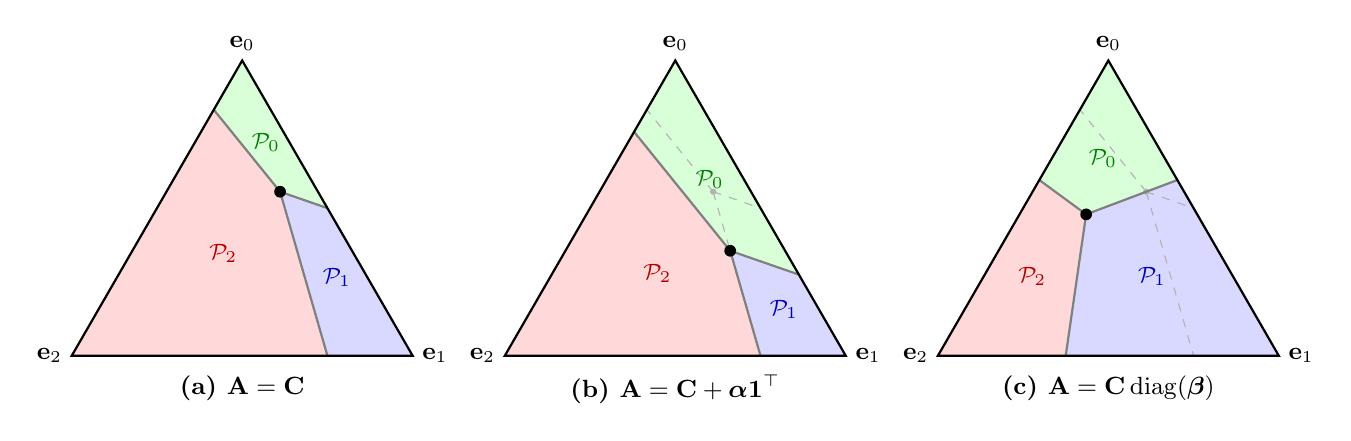
\begin{tikzpicture}[font=\sffamily]

    \begin{scope}[xshift=0.0cm, scale=0.5]
    \coordinate (Top) at (0.000, 5.000);
    \coordinate (Right) at (4.330, -2.500);
    \coordinate (Left) at (-4.330, -2.500);

    \coordinate (Int) at (0.962, 1.667);

    \fill[green!15] (0.000, 5.000) -- (2.165, 1.250) -- (0.962, 1.667) -- (-0.722, 3.750) -- cycle;
    \fill[blue!15] (4.330, -2.500) -- (2.165, -2.500) -- (0.962, 1.667) -- (2.165, 1.250) -- cycle;
    \fill[red!15] (-4.330, -2.500) -- (-0.722, 3.750) -- (0.962, 1.667) -- (2.165, -2.500) -- cycle;

    \draw[thick, black!50] (Int) -- (2.165, 1.250);
    \draw[thick, black!50] (Int) -- (-0.722, 3.750);
    \draw[thick, black!50] (Int) -- (2.165, -2.500);

    \draw[thick] (Top) -- (Right) -- (Left) -- cycle;

    \node[circle, fill=black, inner sep=1.5pt] at (Int) {};

    \node[green!50!black, font=\footnotesize\bfseries] at (0.601, 2.917) {$\mathcal{P}_0$};
    \node[blue!70!black, font=\footnotesize\bfseries] at (2.406, -0.521) {$\mathcal{P}_1$};
    \node[red!70!black, font=\footnotesize\bfseries] at (-0.481, 0.104) {$\mathcal{P}_2$};

    \node[above, font=\small] at (Top) {$\mathbf{e}_0$};
    \node[right, font=\small] at (Right) {$\mathbf{e}_1$};
    \node[left, font=\small] at (Left) {$\mathbf{e}_2$};
    \node[font=\small\bfseries, anchor=north, align=center] at (0, -2.750) {(a) $\mathbf{A} = \mathbf{C}$};
    \end{scope}

    \begin{scope}[xshift=5.5cm, scale=0.5]
    \coordinate (Top) at (0.000, 5.000);
    \coordinate (Right) at (4.330, -2.500);
    \coordinate (Left) at (-4.330, -2.500);

    \coordinate (Int) at (1.395, 0.167);

    \fill[green!15] (0.000, 5.000) -- (3.139, -0.438) -- (1.395, 0.167) -- (-1.046, 3.188) -- cycle;
    \fill[blue!15] (4.330, -2.500) -- (2.165, -2.500) -- (1.395, 0.167) -- (3.139, -0.438) -- cycle;
    \fill[red!15] (-4.330, -2.500) -- (-1.046, 3.188) -- (1.395, 0.167) -- (2.165, -2.500) -- cycle;

    \coordinate (OvInt) at (0.962, 1.667);
    \draw[dashed, gray!60, thin] (OvInt) -- (2.165, 1.250);
    \draw[dashed, gray!60, thin] (OvInt) -- (-0.722, 3.750);
    \draw[dashed, gray!60, thin] (OvInt) -- (2.165, -2.500);
    \node[circle, fill=gray!60, inner sep=0.8pt] at (OvInt) {};

    \draw[thick, black!50] (Int) -- (3.139, -0.438);
    \draw[thick, black!50] (Int) -- (-1.046, 3.188);
    \draw[thick, black!50] (Int) -- (2.165, -2.500);

    \draw[thick] (Top) -- (Right) -- (Left) -- cycle;

    \node[circle, fill=black, inner sep=1.5pt] at (Int) {};

    \node[green!50!black, font=\footnotesize\bfseries] at (0.872, 1.979) {$\mathcal{P}_0$};
    \node[blue!70!black, font=\footnotesize\bfseries] at (2.757, -1.318) {$\mathcal{P}_1$};
    \node[red!70!black, font=\footnotesize\bfseries] at (-0.454, -0.411) {$\mathcal{P}_2$};

    \node[above, font=\small] at (Top) {$\mathbf{e}_0$};
    \node[right, font=\small] at (Right) {$\mathbf{e}_1$};
    \node[left, font=\small] at (Left) {$\mathbf{e}_2$};
    \node[font=\small\bfseries, anchor=north, align=center] at (0, -2.750) {(b) $\mathbf{A} = \mathbf{C} + \boldsymbol{\alpha}\mathbf{1}^\top$};
    \end{scope}

    \begin{scope}[xshift=11.0cm, scale=0.5]
    \coordinate (Top) at (0.000, 5.000);
    \coordinate (Right) at (4.330, -2.500);
    \coordinate (Left) at (-4.330, -2.500);

    \coordinate (Int) at (-0.564, 1.092);

    \fill[green!15] (0.000, 5.000) -- (1.753, 1.964) -- (-0.564, 1.092) -- (-1.753, 1.964) -- cycle;
    \fill[blue!15] (4.330, -2.500) -- (-1.083, -2.500) -- (-0.564, 1.092) -- (1.753, 1.964) -- cycle;
    \fill[red!15] (-4.330, -2.500) -- (-1.753, 1.964) -- (-0.564, 1.092) -- (-1.083, -2.500) -- cycle;

    \coordinate (OvInt) at (0.962, 1.667);
    \draw[dashed, gray!60, thin] (OvInt) -- (2.165, 1.250);
    \draw[dashed, gray!60, thin] (OvInt) -- (-0.722, 3.750);
    \draw[dashed, gray!60, thin] (OvInt) -- (2.165, -2.500);
    \node[circle, fill=gray!60, inner sep=0.8pt] at (OvInt) {};

    \draw[thick, black!50] (Int) -- (1.753, 1.964);
    \draw[thick, black!50] (Int) -- (-1.753, 1.964);
    \draw[thick, black!50] (Int) -- (-1.083, -2.500);

    \draw[thick] (Top) -- (Right) -- (Left) -- cycle;

    \node[circle, fill=black, inner sep=1.5pt] at (Int) {};

    \node[green!50!black, font=\footnotesize\bfseries] at (-0.141, 2.505) {$\mathcal{P}_0$};
    \node[blue!70!black, font=\footnotesize\bfseries] at (1.109, -0.486) {$\mathcal{P}_1$};
    \node[red!70!black, font=\footnotesize\bfseries] at (-1.932, -0.486) {$\mathcal{P}_2$};

    \node[above, font=\small] at (Top) {$\mathbf{e}_0$};
    \node[right, font=\small] at (Right) {$\mathbf{e}_1$};
    \node[left, font=\small] at (Left) {$\mathbf{e}_2$};
    \node[font=\small\bfseries, anchor=north, align=center] at (0, -2.750) {(c) $\mathbf{A} = \mathbf{C}\,\mathrm{diag}(\boldsymbol{\beta})$};
    \end{scope}

\end{tikzpicture}
\end{document}
}
    \caption{Parallel shift versus linear scaling applied to the same asymmetric $\mathbf{C}$ as Figure~\ref{fig:obrien_parallel_shifts}. Panel~(a) is the baseline $\mathbf{A}=\mathbf{C}$. Panel~(b) adds a per-prediction-class bias $\boldsymbol{\alpha}=(-0.30,\,0.15,\,0.15)$: the boundaries translate but retain the normals $\mathbf{n}_{ij}=\mathbf{c}_i-\mathbf{c}_j$ (Proposition~\ref{prop:parallel_invariance}). Panel~(c) applies a linear scaling $\boldsymbol{\beta}=(3.4,\,5.0,\,1.0)$; the dashed baseline shows that the solid boundaries are \emph{rotated}, not merely shifted (Proposition~\ref{prop:column_rotation}). When the cost structure is known, the parallel-shift parameterization respects it by construction; linear scaling does not.}\label{fig:obrien_vs_column_scaling}
\end{figure}

\subsection{Probability ratio thresholding}\label{sec:prob_ratio_thresholding}

An alternative to linear scaling that avoids direct manipulation of the cost matrix is \textit{Probability Ratio Thresholding}, the per-class probability reweighting of \citet{lachiche2003improving}, stated here as a decision rule rather than a probability correction. Rather than modifying the risk computation, this method rescales the estimated probabilities directly,
\begin{equation}\label{eq:threshold_ratio}
    \delta_{\boldsymbol{\tau}}(\mathbf{p}) = \underset{k \in \mathcal{Y}}{\mathrm{argmax}} \; \frac{p_k}{\tau_k},
\end{equation}
where $\boldsymbol{\tau} \in \mathbb{R}_{>0}^K$ is a per-class threshold vector. To remove scale invariance, we fix $\tau_0 = 1$, yielding $K-1$ free parameters.

\begin{proposition}[Equivalence to linear scaling under 0/1 loss]\label{prop:ratio_equivalence}
    Under the 0/1 loss matrix ($C_{ij} = 1 - \delta_{ij}$), Probability Ratio Thresholding with parameter $\boldsymbol{\tau}$ is equivalent to linear scaling with $\beta_k = 1/\tau_k$.
\end{proposition}

\begin{proof}
    Under 0/1 loss, the risk of predicting class $i$ given $\mathbf{p}$ is $\mathcal{L}_i(\mathbf{p}) = \sum_{j \neq i} p_j = 1 - p_i$. The standard analytical rule is $\mathrm{argmin}_{k \in \mathcal{Y}}(1 - p_k) = \mathrm{argmax}_{k \in \mathcal{Y}}\, p_k$. Applying linear scaling with $\boldsymbol{\beta}$ gives $\mathrm{argmin}_{k \in \mathcal{Y}}\sum_{j \neq k} \beta_j p_j = \mathrm{argmin}_{k \in \mathcal{Y}}(\sum_j \beta_j p_j - \beta_k p_k)$. Since $\sum_j \beta_j p_j$ is independent of $k$, this reduces to $\mathrm{argmax}_{k \in \mathcal{Y}}\, \beta_k p_k$. Setting $\beta_k = 1/\tau_k$ yields $\mathrm{argmax}_{k \in \mathcal{Y}}\, p_k / \tau_k$, which is exactly Eq.~\ref{eq:threshold_ratio}.
\end{proof}

Under $0/1$ loss, linear scaling and probability-ratio thresholding thus parameterize the same hypothesis class, the column-scaling counterpart of $\mathcal{H}_{PS}$, which we denote
\begin{equation}\label{eq:hsc_def}
    \mathcal{H}_{Sc} = \left\{ \delta(\mathbf{p}) = \underset{i \in \mathcal{Y}}{\mathrm{argmin}} \sum_{k=0}^{K-1} C_{ki}\, \beta_k\, p_k \;\middle|\; \boldsymbol{\beta} \in \mathbb{R}_{>0}^K,\; \beta_0 = 1 \right\}.
\end{equation}
The gauge $\beta_0 = 1$ pins down the one-dimensional scaling invariance $\arg\min_k(c\, s_k) = \arg\min_k s_k$ for any $c > 0$, so $\mathcal{H}_{Sc}$ has $K-1$ free parameters, the same budget as $\mathcal{H}_{PS}$. Its boundary normals rotate with $\boldsymbol{\beta}$ (Proposition~\ref{prop:column_rotation}) rather than staying fixed at $\mathbf{c}_i - \mathbf{c}_j$, so $\mathcal{H}_{Sc}$ and $\mathcal{H}_{PS}$ are distinct restricted classes at the same complexity, not nested.

\subsection{Multidimensional thresholding}\label{sec:multidim_thresholding}

\citet{legnaro2025multiclass} reformulate the parallel-shift rule directly on the simplex, sidestepping the cost matrix entirely. Their decision rule selects the class with the largest threshold-shifted probability,
\begin{equation}
    \delta(\mathbf{p}) = \underset{k \in \mathcal{Y}}{\mathrm{argmax}} \,\, (p_k - \tau_k),
\end{equation}
parameterized by a threshold vector $\boldsymbol{\tau} \in \Delta^{K-1}$, with the corresponding decision regions
\begin{equation}
    \mathcal{P}_j^{\boldsymbol{\tau}} = \left\{ \mathbf{p} \in \Delta^{K-1} \mid p_j - p_k > \tau_j - \tau_k, \, \forall k \neq j \right\}.
\end{equation}
Unlike probability-ratio thresholding, which rescales the simplex coordinates and rotates the induced boundaries, multidimensional thresholding translates the argmax partition: the pairwise boundaries remain hyperplanes with normals $\mathbf{n}_{ij} = \mathbf{e}_i - \mathbf{e}_j$, but their common intersection is moved away from the barycenter (Figure~\ref{fig:marchetti_thresholding}).

\begin{proposition}[Equivalence to parallel-shift regularization]\label{prop:marchetti_equivalence}
    With the threshold vector allowed to range over $\mathbb{R}^K$, multidimensional thresholding is equivalent to the parallel-shift strategy applied to the $0/1$ loss matrix.
\end{proposition}

\begin{proof}
    Under the $0/1$ cost matrix ($C_{ij} = 1 - \delta_{ij}$), the parallel-shift rule of Section~\ref{sec:partition_optimization} reduces to
    \begin{equation}
        \underset{k \in \mathcal{Y}}{\mathrm{argmin}} \,\, (1 - p_k) + \alpha_k = \underset{k \in \mathcal{Y}}{\mathrm{argmax}} \,\, (p_k - \alpha_k).
    \end{equation}
    Setting $\alpha_k = \tau_k$ recovers the multidimensional-thresholding rule.
\end{proof}

The equivalence is exact only under $0/1$ loss; for asymmetric cost matrices the parallel-shift parameterization on $\mathbf{C}$ exploits cost-matrix structure that the simplex-side $\boldsymbol{\tau}$ does not see.

\begin{figure}[H]
    \centering
    \resizebox{\textwidth}{!}{\documentclass[tikz, border=10pt]{standalone}
\usepackage{tikz}
\usepackage{amsmath}
\usetikzlibrary{shapes, calc, backgrounds, arrows.meta}

\begin{document}
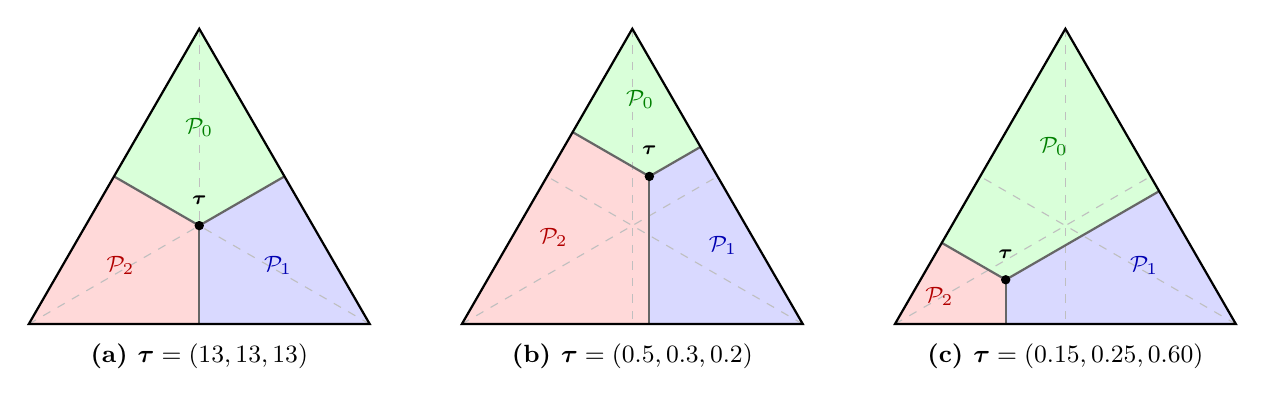
\begin{tikzpicture}[font=\sffamily]

    \begin{scope}[xshift=0.0cm, scale=0.5]
    \coordinate (Top) at (0.000, 5.000);
    \coordinate (Right) at (4.330, -2.500);
    \coordinate (Left) at (-4.330, -2.500);

    \coordinate (Int) at (0.000, 0.000);

    \fill[green!15] (0.000, 5.000) -- (2.165, 1.250) -- (0.000, 0.000) -- (-2.165, 1.250) -- cycle;
    \fill[blue!15] (4.330, -2.500) -- (0.000, -2.500) -- (0.000, 0.000) -- (2.165, 1.250) -- cycle;
    \fill[red!15] (-4.330, -2.500) -- (-2.165, 1.250) -- (0.000, 0.000) -- (0.000, -2.500) -- cycle;

    \draw[dashed, gray!50, thin] (Left) -- (2.165, 1.250);
    \draw[dashed, gray!50, thin] (Right) -- (-2.165, 1.250);
    \draw[dashed, gray!50, thin] (Top) -- (0.000, -2.500);

    \draw[thick, black!60] (Int) -- (2.165, 1.250);
    \draw[thick, black!60] (Int) -- (-2.165, 1.250);
    \draw[thick, black!60] (Int) -- (0.000, -2.500);

    \node[circle, fill=black, inner sep=1.2pt] at (Int) {};
    \node[font=\scriptsize, anchor=south] at (0.000, 0.300) {$\boldsymbol{\tau}$};

    \draw[thick] (Top) -- (Right) -- (Left) -- cycle;

    \node[green!50!black, font=\footnotesize\bfseries] at (0.000, 2.500) {$\mathcal{P}_0$};
    \node[blue!70!black, font=\footnotesize\bfseries] at (2.000, -1.000) {$\mathcal{P}_1$};
    \node[red!70!black, font=\footnotesize\bfseries] at (-2.000, -1.000) {$\mathcal{P}_2$};

    \node[font=\small\bfseries, anchor=north, align=center] at (0, -2.750) {(a) $\boldsymbol{\tau} = (\tfrac{1}{3},\tfrac{1}{3},\tfrac{1}{3})$};
    \end{scope}

    \begin{scope}[xshift=5.5cm, scale=0.5]
    \coordinate (Top) at (0.000, 5.000);
    \coordinate (Right) at (4.330, -2.500);
    \coordinate (Left) at (-4.330, -2.500);

    \coordinate (Int) at (0.433, 1.250);

    \fill[green!15] (0.000, 5.000) -- (1.732, 2.000) -- (0.433, 1.250) -- (-1.516, 2.375) -- cycle;
    \fill[blue!15] (4.330, -2.500) -- (0.433, -2.500) -- (0.433, 1.250) -- (1.732, 2.000) -- cycle;
    \fill[red!15] (-4.330, -2.500) -- (-1.516, 2.375) -- (0.433, 1.250) -- (0.433, -2.500) -- cycle;

    \draw[dashed, gray!50, thin] (Left) -- (2.165, 1.250);
    \draw[dashed, gray!50, thin] (Right) -- (-2.165, 1.250);
    \draw[dashed, gray!50, thin] (Top) -- (0.000, -2.500);

    \draw[thick, black!60] (Int) -- (1.732, 2.000);
    \draw[thick, black!60] (Int) -- (-1.516, 2.375);
    \draw[thick, black!60] (Int) -- (0.433, -2.500);

    \node[circle, fill=black, inner sep=1.2pt] at (Int) {};
    \node[font=\scriptsize, anchor=south] at (0.433, 1.550) {$\boldsymbol{\tau}$};

    \draw[thick] (Top) -- (Right) -- (Left) -- cycle;

    \node[green!50!black, font=\footnotesize\bfseries] at (0.200, 3.200) {$\mathcal{P}_0$};
    \node[blue!70!black, font=\footnotesize\bfseries] at (2.300, -0.500) {$\mathcal{P}_1$};
    \node[red!70!black, font=\footnotesize\bfseries] at (-2.000, -0.300) {$\mathcal{P}_2$};

    \node[font=\small\bfseries, anchor=north, align=center] at (0, -2.750) {(b) $\boldsymbol{\tau} = (0.5, 0.3, 0.2)$};
    \end{scope}

    \begin{scope}[xshift=11.0cm, scale=0.5]
    \coordinate (Top) at (0.000, 5.000);
    \coordinate (Right) at (4.330, -2.500);
    \coordinate (Left) at (-4.330, -2.500);

    \coordinate (Int) at (-1.516, -1.375);

    \fill[green!15] (0.000, 5.000) -- (2.382, 0.875) -- (-1.516, -1.375) -- (-3.139, -0.438) -- cycle;
    \fill[blue!15] (4.330, -2.500) -- (-1.516, -2.500) -- (-1.516, -1.375) -- (2.382, 0.875) -- cycle;
    \fill[red!15] (-4.330, -2.500) -- (-3.139, -0.438) -- (-1.516, -1.375) -- (-1.516, -2.500) -- cycle;

    \draw[dashed, gray!50, thin] (Left) -- (2.165, 1.250);
    \draw[dashed, gray!50, thin] (Right) -- (-2.165, 1.250);
    \draw[dashed, gray!50, thin] (Top) -- (0.000, -2.500);

    \draw[thick, black!60] (Int) -- (2.382, 0.875);
    \draw[thick, black!60] (Int) -- (-3.139, -0.438);
    \draw[thick, black!60] (Int) -- (-1.516, -2.500);

    \node[circle, fill=black, inner sep=1.2pt] at (Int) {};
    \node[font=\scriptsize, anchor=south] at (-1.516, -1.075) {$\boldsymbol{\tau}$};

    \draw[thick] (Top) -- (Right) -- (Left) -- cycle;

    \node[green!50!black, font=\footnotesize\bfseries] at (-0.300, 2.000) {$\mathcal{P}_0$};
    \node[blue!70!black, font=\footnotesize\bfseries] at (2.000, -1.000) {$\mathcal{P}_1$};
    \node[red!70!black, font=\footnotesize\bfseries] at (-3.200, -1.800) {$\mathcal{P}_2$};

    \node[font=\small\bfseries, anchor=north, align=center] at (0, -2.750) {(c) $\boldsymbol{\tau} = (0.15, 0.25, 0.60)$};
    \end{scope}

\end{tikzpicture}
\end{document}
}
    \caption{Effect of the threshold vector $\boldsymbol{\tau}$ on the multidimensional thresholding rule. The decision rule $\delta(\mathbf{p}) = \operatorname{argmax}_{k \in \mathcal{Y}} (p_k - \tau_k)$ produces boundaries parallel to the argmax medians (dashed gray), with the intersection point shifted from the barycenter $G$ to $\boldsymbol{\tau}$ (black dot). A larger $\tau_k$ penalizes class~$k$, shrinking $\mathcal{P}_k^{\boldsymbol{\tau}}$: \textbf{(a)}~equal thresholds recover the standard argmax partition; \textbf{(b)}~$\tau_0 = 0.5$ shrinks $\mathcal{P}_0^{\boldsymbol{\tau}}$; \textbf{(c)}~$\tau_2 = 0.60$ shrinks $\mathcal{P}_2^{\boldsymbol{\tau}}$, expanding $\mathcal{P}_0^{\boldsymbol{\tau}}$.}\label{fig:marchetti_thresholding}
\end{figure}

\citeauthor{obrien2008costsensitive}'s parallel shifts and \citeauthor{legnaro2025multiclass}'s multidimensional thresholding are thus the same restricted class when $\boldsymbol{\tau}$ ranges over $\mathbb{R}^K$, in which boundaries are parameterized by a single vector $\mathbf{v} \in \mathbb{R}^K$ (either the bias $\boldsymbol{\alpha}$ or the threshold $\boldsymbol{\tau}$),
\begin{equation}\label{eq:hps_def}
    \mathcal{H}_{PS} = \left\{ \delta(\mathbf{p}) = \underset{k \in \mathcal{Y}}{\mathrm{argmin}} \,\, (\mathbf{c}_k^\top \mathbf{p} + v_k) \mid \mathbf{v} \in \mathbb{R}^{K}, \sum v_k = 0 \right\}.
\end{equation}
The mean-zero gauge $\sum_k v_k = 0$ pins down the one-dimensional translation invariance $\arg\min_{k \in \mathcal{Y}}(s_k + c) = \arg\min_{k \in \mathcal{Y}} s_k$ for any scalar $c$. The accompanying code adopts the equivalent first-coordinate gauge $v_0 = 0$ instead and searches the remaining $K-1$ coordinates; the two parameterizations yield identical decision rules but the recorded bias vectors differ by the additive constant $-\overline{v}$. Linear scaling (Section~\ref{sec:linear_scaling}) and probability-ratio thresholding (Section~\ref{sec:prob_ratio_thresholding}) form the column-scaling sibling $\mathcal{H}_{Sc}$ (Eq.~\ref{eq:hsc_def}) at the same $K-1$ parameter budget but outside $\mathcal{H}_{PS}$: their boundary normals are rotated by the per-class scaling (Proposition~\ref{prop:column_rotation}) rather than fixed at $\mathbf{c}_i - \mathbf{c}_j$.

\subsection{Priority-based sequential selection}\label{sec:sequential_selection}

An alternative heuristic, motivated by class-imbalanced settings, applies per-class binary thresholds in a sequential cascade that processes classes in an explicit priority order. This construction is not new: structurally the rule is a decision list \citep{rivest1987decision}, an ordered sequence of tests in which the first satisfied test fixes the label and an explicit default applies when none fire. Each test $p_k \ge \tau_k$ is a one-vs-rest detector \citep{rifkin2004defense}, so the cascade can equivalently be read as a one-vs-rest decomposition in which several simultaneously firing detectors are disambiguated by a fixed class priority rather than by the usual argmax combination. We present it here mainly to contrast it with the convex-polytope methods above; the first-match-with-default structure that defines a decision list yields the non-convex, order-dependent geometry analysed below.

Let $\mathrm{ord}: \mathcal{Y} \to \mathcal{Y}$ be a permutation defining the evaluation order (for the imbalanced motivation, classes sorted by ascending training frequency, so rare classes are evaluated first), and let $\boldsymbol{\tau} \in [0,1]^K$ be a vector of per-class probability thresholds. The decision rule is
\begin{equation}\label{eq:sequential_selection}
    \delta_{\mathrm{ord}, \boldsymbol{\tau}}(\mathbf{p}) = \begin{cases}
        \mathrm{ord}(j^*) & \text{if } j^* = \min\{j \in \{0, \ldots, K{-}1\} \mid p_{\mathrm{ord}(j)} \geq \tau_{\mathrm{ord}(j)}\} \text{ exists}, \\
        \mathrm{argmax}_{k \in \mathcal{Y}}\, p_k & \text{otherwise}.
    \end{cases}
\end{equation}
The first class in the priority ordering whose probability exceeds its threshold is selected; if no threshold is met, the standard argmax rule applies as a default. The ordering $\mathrm{ord}$ encodes an application-defined priority and is not tied to the frequency-based choice; any domain ranking is admissible, including one derived from the cost matrix $\mathbf{C}$. Sorting classes by descending worst-case misclassification cost $\max_{j \neq k} C_{kj}$, for example, places the classes most expensive to miss earliest in the cascade, so such a class claims an instance whenever its threshold is met even when a less costly class has larger estimated probability.

The decision regions induced by Eq.~\ref{eq:sequential_selection} differ qualitatively from those of every preceding method: they are \emph{not} convex polytopes, and they depend on the evaluation order $\mathrm{ord}$. Because a class is selected as soon as its own threshold is met, a class placed earlier in the ordering can claim an instance even when a later class has larger estimated probability. The cascade therefore implements an explicit priority rule, and under the frequency-based ordering it ensures that rare classes are considered before common ones. Figure~\ref{fig:sequential_selection} shows the resulting non-convex, order-dependent regions.

The rule has $K$ free parameters, one threshold per class, compared with $K-1$ for the vector-tuned classes of Section~\ref{sec:partition_optimization}. Its capacity is not directly comparable to theirs: the non-convex, order-dependent regions do not admit the Natarajan-dimension argument used for the convex-polytope classes, so the method carries no analogous sample-complexity guarantee.

\begin{figure}[H]
    \centering
    \documentclass[tikz, border=10pt]{standalone}
\usepackage{tikz}
\usepackage{amsmath}
\usetikzlibrary{calc, arrows.meta}

\begin{document}
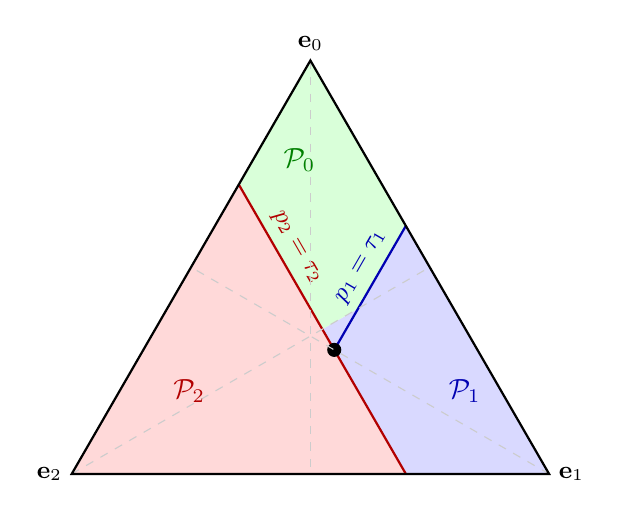
\begin{tikzpicture}[font=\sffamily, scale=0.7]

    % Vertices
    \coordinate (T) at (0, 5);          % Class 0 (p_0=1)
    \coordinate (R) at (4.33, -2.5);    % Class 1 (p_1=1)
    \coordinate (L) at (-4.33, -2.5);   % Class 2 (p_2=1)

    % Threshold contour endpoints:
    % p_2 = 0.30 line:
    %   Top-Left edge (p_1=0): (0.70, 0, 0.30) -> (-1.299, 2.75)
    %   Right-Left edge (p_0=0): (0, 0.70, 0.30) -> (1.732, -2.5)
    \coordinate (T2a) at (-1.299, 2.75);
    \coordinate (T2b) at (1.732, -2.5);

    % p_1 = 0.40 line:
    %   Top-Right edge (p_2=0): (0.60, 0.40, 0) -> (1.732, 2.0)
    %   Right-Left edge (p_0=0): (0, 0.40, 0.60) -> (-0.866, -2.5)
    \coordinate (T1a) at (1.732, 2.0);
    \coordinate (T1b) at (-0.866, -2.5);

    % Intersection of p_2=0.30 and p_1=0.40: (0.30, 0.40, 0.30) -> (0.433, -0.25)
    \coordinate (Corner) at (0.433, -0.25);

    % ===== Region fills =====

    % Argmax median (p_0=p_1) intersects the fallback region at two points:
    %   MedOnBlue: on p_1=0.40 line at (0.35, 0.35, 0.30) -> (0.2165, 0.125)
    %     Wait: (p0=0.35, p1=0.35, p2=0.30) -> x=4.33*(0.35-0.30)=0.2165, y=7.5*0.35-2.5=0.125
    %   MedOnP1: on p_1=0.40 line at (0.30, 0.40, 0.30)... that's Corner itself
    %     Actually: median L-MidTR intersects p_1=0.40 at (0.30, 0.40, 0.30)
    %     but Corner=(0.30, 0.40, 0.30) IS the intersection of p1=0.40 and p2=0.30.
    %     The median hits p_1=0.40 at (p0, 0.40, p2) where p0=p1=0.40... wait no.
    %     p0=p1 and p1=0.40 means p0=0.40, p2=0.20.
    %     -> x=4.33*(0.40-0.20)=0.866, y=7.5*0.40-2.5=0.5
    \coordinate (MedOnRed) at (0.2165, 0.125);  % p0=p1 meets p2=0.30
    \coordinate (MedOnBlue) at (0.866, 0.5);     % p0=p1 meets p1=0.40

    % Class 2 (red, priority 1): p_2 >= 0.30
    \fill[red!15] (T2a) -- (T2b) -- (L) -- cycle;

    % Class 1 (blue, priority 2): p_2 < 0.30 AND p_1 >= 0.40
    \fill[blue!15] (T1a) -- (Corner) -- (T2b) -- (R) -- cycle;

    % Class 1 (blue, fallback argmax): p_2 < 0.30 AND p_1 < 0.40 AND p_1 > p_0
    \fill[blue!15] (MedOnBlue) -- (Corner) -- (MedOnRed) -- cycle;

    % Class 0 (green, fallback argmax): p_2 < 0.30 AND p_1 < 0.40 AND p_0 > p_1
    \fill[green!15] (T) -- (T1a) -- (MedOnBlue) -- (MedOnRed) -- (T2a) -- cycle;

    % ===== Threshold contour lines =====

    % p_2 = tau_2 line (separates class 2 from rest)
    \draw[thick, red!70!black] (T2a) -- (T2b)
        node[sloped, above, pos=0.25, font=\small, red!70!black] {$p_2 = \tau_2$};

    % p_1 = tau_1 line (separates class 1 from class 0, within p_2 < tau_2)
    \draw[thick, blue!70!black] (T1a) -- (Corner)
        node[sloped, above, pos=0.4, font=\small, blue!70!black] {$p_1 = \tau_1$};

    % Corner marker (the "step" — key visual)
    \node[circle, fill=black, inner sep=1.8pt] at (Corner) {};

    % ===== Argmax boundaries (dashed, for comparison) =====
    \coordinate (MidTR) at (2.165, 1.25);
    \coordinate (MidTL) at (-2.165, 1.25);
    \coordinate (MidRL) at (0, -2.5);
    \draw[dashed, gray!40, thin] (L) -- (MidTR);
    \draw[dashed, gray!40, thin] (R) -- (MidTL);
    \draw[dashed, gray!40, thin] (T) -- (MidRL);

    % ===== Triangle frame =====
    \draw[thick] (T) -- (R) -- (L) -- cycle;

    % ===== Labels =====

    % Vertex labels
    \node[above, font=\small] at (T) {$\mathbf{e}_0$};
    \node[right, font=\small] at (R) {$\mathbf{e}_1$};
    \node[left, font=\small] at (L) {$\mathbf{e}_2$};

    % Region labels
    \node[green!50!black, font=\normalsize\bfseries] at (-0.2, 3.2) {$\mathcal{P}_0$};
    \node[blue!70!black, font=\normalsize\bfseries] at (2.8, -1.0) {$\mathcal{P}_1$};
    \node[red!70!black, font=\normalsize\bfseries] at (-2.2, -1.0) {$\mathcal{P}_2$};

\end{tikzpicture}
\end{document}

    \caption{Decision regions induced by sequential selection with priority order $\mathrm{ord} = (2, 1, 0)$ and thresholds $\tau_2 = 0.30$, $\tau_1 = 0.40$ on the 3-class probability simplex. Class~2 is evaluated first: any point with $p_2 \ge \tau_2$ is claimed by class~2 regardless of other probabilities, creating the red region. Class~1 is evaluated next in the complement, and class~0 receives the fallback.}\label{fig:sequential_selection}
\end{figure}

\section{Limitations of parallel-shift partitions}

Every boundary normal of $\mathcal{H}_{PS}$ is locked to $\mathbf{n}_{ij} = \mathbf{c}_i - \mathbf{c}_j$, a fixed expressivity cost: the rule can translate the partition but cannot rotate or curve any boundary. Two regimes make this constraint binding.

\subsection{Error-covariance misalignment}
When the estimator's error has directional structure that is not aligned with the cost-matrix differences, the risk-minimizing boundary in estimate space need not be normal to $\mathbf{n}_{ij} = \mathbf{c}_i - \mathbf{c}_j$. If $\Sigma_\epsilon$ is the covariance of $\boldsymbol{\epsilon}(x) = \hat{\mathbf{p}}(x) - \boldsymbol{\eta}(x)$ and its principal axes are not aligned with $\mathbf{c}_i - \mathbf{c}_j$, the orientation that minimizes risk depends on $\Sigma_\epsilon$ and can differ from the analytical normal. $\mathcal{H}_{PS}$ fixes every boundary normal at $\mathbf{n}_{ij}$, so it cannot represent such a rotation and the mismatch contributes to excess risk that the class has no parameter to remove.

\subsection{Non-linear calibration bias}
When the systematic distortion $\Psi$ of Section~\ref{sec:analytical_fragility} is non-linear (for example the saturation of softmax outputs in deep networks, or the prior shrinkage of in-context predictors), the pre-image $\Psi^{-1}(\mathcal{B}_{ij})$ of the analytical boundary is in general a curved manifold in estimate space rather than a hyperplane. A flat parallel-shift boundary can only approximate it, with an approximation error that grows with the local curvature of $\Psi$ and that $\mathcal{H}_{PS}$ has no parameter to reduce.

Both regimes motivate a hypothesis class whose boundary normals can rotate, which $\mathcal{H}_{PS}$ forbids. The Voronoi partition class of Chapter~\ref{sec:voronoi_tessellation} provides this, with $K(K-1)$ prototype parameters and boundary rotations that $\mathcal{H}_{PS}$ cannot represent.

%!TeX root=../carlo_master.tex
\chapter{Voronoi tessellations as decision hypothesis class}\label{sec:voronoi_tessellation}

The parallel-shift class $\mathcal{H}_{PS}$ is structured but rigid: its boundary normals are fixed at $\mathbf{c}_i-\mathbf{c}_j$, so learning can only translate the partition. The full class $\mathcal{H}_{Full}$ removes this rigidity by freeing every pairwise boundary, but loses the coupling of a coherent multiclass geometry. This chapter studies a candidate intermediate class, the Voronoi one: its boundaries can rotate, but only through the motion of $K$ shared class prototypes. Moving one prototype changes all boundaries involving that class, so the pairwise decisions are regularized by a common geometric representation.

\section{From argmax to the Voronoi parameterization}

The standard cost-blind argmax rule is already a nearest-prototype rule on the simplex. The squared Euclidean distance from $\mathbf{p}$ to a vertex $\mathbf{e}_i$ is $\|\mathbf{p} - \mathbf{e}_i\|_2^2 = \|\mathbf{p}\|_2^2 - 2 p_i + 1$, in which only the $-2 p_i$ term depends on $i$, so $\arg\min_{i \in \mathcal{Y}} \|\mathbf{p} - \mathbf{e}_i\|_2^2 = \arg\max_{i \in \mathcal{Y}} p_i$. Assigning each $\mathbf{p}$ to its nearest vertex therefore reproduces the Bayes rule under $0/1$ loss, and the induced partition of $\Delta^{K-1}$ is the tessellation into cells closest to each vertex $\{\mathbf{e}_0, \ldots, \mathbf{e}_{K-1}\}$.

Nothing in this construction forces the reference points to sit at the vertices. The vertices are the natural anchors only because argmax treats class $k$ as fully described by $\mathbf{e}_k$; once the estimator's outputs are distorted (Section~\ref{sec:analytical_fragility}), that choice need no longer be the one that minimizes risk. Letting the $K$ prototypes move freely inside the simplex gives a strictly richer family of partitions, parameterized by the prototype locations rather than by hyperplane coefficients. The rest of this section makes that family precise and studies its expressivity and sample complexity.

\section{The Voronoi decision rule}

Let $\mathcal{M} = \{ \boldsymbol{\mu}_0, \boldsymbol{\mu}_1, \dots, \boldsymbol{\mu}_{K-1} \}$ be a set of $K$ distinct prototypes, where $\boldsymbol{\mu}_k \in \mathbb{R}^K$ is the learnable anchor for class $k$.

\begin{definition}[Voronoi decision rule]
    The decision rule $\delta_{\mathcal{M}}: \Delta^{K-1} \to \mathcal{Y}$ assigns a probability vector $\mathbf{p}$ to the class of its nearest prototype,
    \begin{equation}\label{eq:voronoi_rule}
        \delta_{\mathcal{M}}(\mathbf{p}) = \underset{k \in \mathcal{Y}}{\mathrm{argmin}} \, \| \mathbf{p} - \boldsymbol{\mu}_k \|_2.
    \end{equation}
\end{definition}

This rule induces a Voronoi tessellation of the simplex: the decision region $\mathcal{P}_k^{\mathcal{M}}$ is the convex cell of points in $\Delta^{K-1}$ closer to $\boldsymbol{\mu}_k$ than to any other prototype.

The boundary between classes $i$ and $j$ is the perpendicular bisector of the segment joining $\boldsymbol{\mu}_i$ and $\boldsymbol{\mu}_j$. Equivalently, it is the set of $\mathbf{p}$ satisfying
\begin{equation}
    \|\mathbf{p}-\boldsymbol{\mu}_i\|_2^2 = \|\mathbf{p}-\boldsymbol{\mu}_j\|_2^2,
\end{equation}
or
\begin{equation}
    2(\boldsymbol{\mu}_i-\boldsymbol{\mu}_j)^\top \mathbf{p} = \|\boldsymbol{\mu}_i\|_2^2-\|\boldsymbol{\mu}_j\|_2^2.
\end{equation}
Thus the Voronoi boundary normal is
\begin{equation}
    \mathbf{n}_{vor} = \boldsymbol{\mu}_i - \boldsymbol{\mu}_j.
\end{equation}
Unlike in $\mathcal{H}_{PS}$, where the corresponding normal is fixed by the cost matrix at $\mathbf{c}_i-\mathbf{c}_j$, the Voronoi normal can rotate as the prototypes move. Moving a prototype also shifts all boundaries involving that class, coupling the pairwise decisions through a common geometric representation.

This prototype view also explains the role of interior anchors. When the estimator contracts probability mass toward the barycenter (Section~\ref{sec:analytical_fragility}), the simplex vertices may lie outside the effective support of $\hat{\mathbf{p}}$. The argmax Voronoi diagram generated by $\{\mathbf{e}_0,\ldots,\mathbf{e}_{K-1}\}$ then partitions regions that the estimator rarely visits. Moving the prototypes into the simplex interior places the decision boundaries within the support of the estimated probabilities and allows both boundary translation and rotation. Figure~\ref{fig:partition_strategies} compares this geometry with the parallel-shift alternative.


\begin{figure}[H]
    \centering
    \resizebox{0.65\textwidth}{!}{\documentclass[tikz, border=10pt]{standalone}
\usepackage{tikz}
\usepackage{amsmath}
\usetikzlibrary{shapes, calc, backgrounds, arrows.meta}

\begin{document}
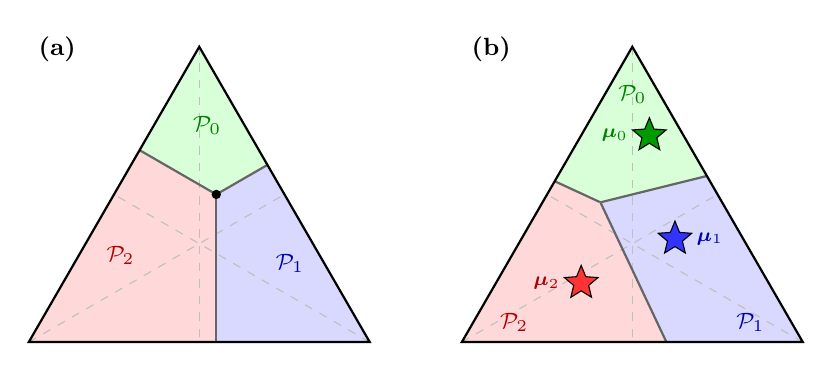
\begin{tikzpicture}[font=\sffamily]

    \begin{scope}[xshift=0.0cm, scale=0.5]
    \node[font=\small\bfseries, anchor=north west] at (-4.330, 5.500) {(a)};
    \coordinate (Top) at (0.000, 5.000);
    \coordinate (Right) at (4.330, -2.500);
    \coordinate (Left) at (-4.330, -2.500);

    \coordinate (Int) at (0.433, 1.250);

    \fill[green!15] (0.000, 5.000) -- (1.732, 2.000) -- (0.433, 1.250) -- (-1.516, 2.375) -- cycle;
    \fill[blue!15] (4.330, -2.500) -- (0.433, -2.500) -- (0.433, 1.250) -- (1.732, 2.000) -- cycle;
    \fill[red!15] (-4.330, -2.500) -- (-1.516, 2.375) -- (0.433, 1.250) -- (0.433, -2.500) -- cycle;

    \draw[dashed, gray!50, thin] (Left) -- (2.165, 1.250);
    \draw[dashed, gray!50, thin] (Right) -- (-2.165, 1.250);
    \draw[dashed, gray!50, thin] (Top) -- (0.000, -2.500);

    \draw[thick, black!60] (Int) -- (1.732, 2.000);
    \draw[thick, black!60] (Int) -- (-1.516, 2.375);
    \draw[thick, black!60] (Int) -- (0.433, -2.500);

    \node[circle, fill=black, inner sep=1.2pt] at (Int) {};

    \draw[thick] (Top) -- (Right) -- (Left) -- cycle;

    \node[green!50!black, font=\footnotesize\bfseries] at (0.200, 3.000) {$\mathcal{P}_0$};
    \node[blue!70!black, font=\footnotesize\bfseries] at (2.300, -0.500) {$\mathcal{P}_1$};
    \node[red!70!black, font=\footnotesize\bfseries] at (-2.000, -0.300) {$\mathcal{P}_2$};

    \end{scope}

    \begin{scope}[xshift=5.5cm, scale=0.5]
    \node[font=\small\bfseries, anchor=north west] at (-4.330, 5.500) {(b)};
    \coordinate (Top) at (0.000, 5.000);
    \coordinate (Right) at (4.330, -2.500);
    \coordinate (Left) at (-4.330, -2.500);

    \coordinate (Mu0) at (0.433, 2.750);
    \coordinate (Mu1) at (1.083, 0.125);
    \coordinate (Mu2) at (-1.299, -1.000);

    % Region 0 (Green)
    \begin{scope}
        \clip (Top) -- (Right) -- (Left) -- cycle;
        \path (Mu0) -- (Mu1) coordinate[midway] (M01);
        \clip ($(M01)!20cm!90:(Mu1)$) -- ($(M01)!20cm!-90:(Mu1)$) -- ($(M01)!20cm!180:(Mu1)$) -- cycle;
        \path (Mu0) -- (Mu2) coordinate[midway] (M02);
        \clip ($(M02)!20cm!90:(Mu2)$) -- ($(M02)!20cm!-90:(Mu2)$) -- ($(M02)!20cm!180:(Mu2)$) -- cycle;
        \fill[green!15] (-6,-6) rectangle (6,6);
    \end{scope}

    % Region 1 (Blue)
    \begin{scope}
        \clip (Top) -- (Right) -- (Left) -- cycle;
        \path (Mu1) -- (Mu0) coordinate[midway] (M10);
        \clip ($(M10)!20cm!90:(Mu0)$) -- ($(M10)!20cm!-90:(Mu0)$) -- ($(M10)!20cm!180:(Mu0)$) -- cycle;
        \path (Mu1) -- (Mu2) coordinate[midway] (M12);
        \clip ($(M12)!20cm!90:(Mu2)$) -- ($(M12)!20cm!-90:(Mu2)$) -- ($(M12)!20cm!180:(Mu2)$) -- cycle;
        \fill[blue!15] (-6,-6) rectangle (6,6);
    \end{scope}

    % Region 2 (Red)
    \begin{scope}
        \clip (Top) -- (Right) -- (Left) -- cycle;
        \path (Mu2) -- (Mu0) coordinate[midway] (M20);
        \clip ($(M20)!20cm!90:(Mu0)$) -- ($(M20)!20cm!-90:(Mu0)$) -- ($(M20)!20cm!180:(Mu0)$) -- cycle;
        \path (Mu2) -- (Mu1) coordinate[midway] (M21);
        \clip ($(M21)!20cm!90:(Mu1)$) -- ($(M21)!20cm!-90:(Mu1)$) -- ($(M21)!20cm!180:(Mu1)$) -- cycle;
        \fill[red!15] (-6,-6) rectangle (6,6);
    \end{scope}

    \draw[dashed, gray!50, thin] (Left) -- (2.165, 1.250);
    \draw[dashed, gray!50, thin] (Right) -- (-2.165, 1.250);
    \draw[dashed, gray!50, thin] (Top) -- (0.000, -2.500);

    \begin{scope}
        \clip (Top) -- (Right) -- (Left) -- cycle;
        \path (Mu0) -- (Mu2) coordinate[midway] (Mc02);
        \clip ($(Mc02)!20cm!90:(Mu2)$) -- ($(Mc02)!20cm!-90:(Mu2)$) -- ($(Mc02)!20cm!180:(Mu2)$) -- cycle;
        \path (Mu0) -- (Mu1) coordinate[midway] (Mb01);
        \draw[thick, black!60] ($(Mb01)!20cm!90:(Mu1)$) -- ($(Mb01)!20cm!-90:(Mu1)$);
    \end{scope}
    \begin{scope}
        \clip (Top) -- (Right) -- (Left) -- cycle;
        \path (Mu0) -- (Mu1) coordinate[midway] (Mc01);
        \clip ($(Mc01)!20cm!90:(Mu1)$) -- ($(Mc01)!20cm!-90:(Mu1)$) -- ($(Mc01)!20cm!180:(Mu1)$) -- cycle;
        \path (Mu0) -- (Mu2) coordinate[midway] (Mb02);
        \draw[thick, black!60] ($(Mb02)!20cm!90:(Mu2)$) -- ($(Mb02)!20cm!-90:(Mu2)$);
    \end{scope}
    \begin{scope}
        \clip (Top) -- (Right) -- (Left) -- cycle;
        \path (Mu1) -- (Mu0) coordinate[midway] (Mc10);
        \clip ($(Mc10)!20cm!90:(Mu0)$) -- ($(Mc10)!20cm!-90:(Mu0)$) -- ($(Mc10)!20cm!180:(Mu0)$) -- cycle;
        \path (Mu1) -- (Mu2) coordinate[midway] (Mb12);
        \draw[thick, black!60] ($(Mb12)!20cm!90:(Mu2)$) -- ($(Mb12)!20cm!-90:(Mu2)$);
    \end{scope}

    \draw[thick] (Top) -- (Right) -- (Left) -- cycle;

    \node[star, star points=5, star point ratio=2.25, fill=green!60!black, draw=black, inner sep=2pt] at (Mu0) {};
    \node[font=\scriptsize, green!50!black, anchor=east] at ($(Mu0)+(-0.300,0.000)$) {$\boldsymbol{\mu}_0$};
    \node[star, star points=5, star point ratio=2.25, fill=blue!80, draw=black, inner sep=2pt] at (Mu1) {};
    \node[font=\scriptsize, blue!70!black, anchor=west] at ($(Mu1)+(0.300,0.000)$) {$\boldsymbol{\mu}_1$};
    \node[star, star points=5, star point ratio=2.25, fill=red!80, draw=black, inner sep=2pt] at (Mu2) {};
    \node[font=\scriptsize, red!70!black, anchor=east] at ($(Mu2)+(-0.300,0.000)$) {$\boldsymbol{\mu}_2$};

    \node[green!50!black, font=\footnotesize\bfseries] at (0.000, 3.800) {$\mathcal{P}_0$};
    \node[blue!70!black, font=\footnotesize\bfseries] at (3.000, -2.000) {$\mathcal{P}_1$};
    \node[red!70!black, font=\footnotesize\bfseries] at (-3.000, -2.000) {$\mathcal{P}_2$};

    \end{scope}

\end{tikzpicture}
\end{document}
}
    \caption{Geometric comparison of partition optimization strategies on the 3-class simplex. Dashed gray lines show the baseline argmax boundaries (medians meeting at the barycenter). \textbf{(a)}~Parallel Shift preserves boundary orientations (fixed normals $\mathbf{n}_{ij} = \mathbf{e}_i - \mathbf{e}_j$) and translates the intersection point, using $K{-}1$ free parameters. \textbf{(b)}~Voronoi tessellation places free prototypes $\boldsymbol{\mu}_k$ inside the simplex, allowing both rotation and translation with $K(K{-}1)$ parameters.}\label{fig:partition_strategies}
\end{figure}

We will use two versions of the class. For expressivity results, prototypes are allowed anywhere in $\mathbb{R}^K$; this unconstrained class is denoted $\mathcal{H}_{Vor}$. For the optimizer, prototypes are restricted to the simplex, giving $\mathcal{H}_{Vor}^{\Delta}$. The restriction matches the interpretation of prototypes as probability-space anchors, but it is not only cosmetic: the containment result for $\mathcal{H}_{PS}$ uses off-simplex prototypes and therefore applies to $\mathcal{H}_{Vor}$, not necessarily to $\mathcal{H}_{Vor}^{\Delta}$.

\section{Containment and strict separation from the parallel-shift class}

The preceding paragraphs established the geometry: the parallel-shift normal $\mathbf{n}_{ps} = \mathbf{c}_i - \mathbf{c}_j$ is fixed by the cost matrix, while the Voronoi normal $\mathbf{n}_{vor} = \boldsymbol{\mu}_i - \boldsymbol{\mu}_j$ rotates freely with the prototypes. We now establish what that freedom buys at the population level: $\mathcal{H}_{Vor}$ contains $\mathcal{H}_{PS}$ and represents partitions it cannot (Theorem~\ref{thm:rotational_dominance}, Proposition~\ref{prop:ps_in_vor}), an unconditional property of the function classes. Whether the resulting advantage is realized under a given estimator is a separate, finite-sample question.

The separation is unconditional. It uses symmetric $0/1$ loss, so the parallel-shift normals carry no cost-matrix information and no estimator distortion enters; the comparison isolates pure boundary geometry. We exhibit a single 3-class point configuration, a ``vertical stack'' along the simplex altitude, on which $\mathcal{H}_{PS}$ incurs irreducible positive risk while a Voronoi partition with prototypes in $\mathcal{H}_{Vor}^{\mathrm{DLC}}$ achieves zero risk.

\begin{theorem}[Strict risk separation from the parallel-shift class]\label{thm:rotational_dominance}
    Let $\mathcal{H}_{PS}$ be the class of parallel-shift partitions and let $\mathcal{H}_{Vor}^{\mathrm{DLC}} \subseteq \mathcal{H}_{Vor}$ be the subclass of Voronoi partitions whose prototypes satisfy the pure-class vertex-consistency condition
    \begin{equation}
        \arg\min_{j \in \mathcal{Y}} \, \|\mathbf{e}_k - \boldsymbol{\mu}_j\|_2 = \{k\} \qquad \text{for every } k \in \mathcal{Y},
        \label{eq:thm_vertex_consistency}
    \end{equation}
    so that the Voronoi decoder agrees with argmax decoding at every simplex vertex. (This is the Dominant Label Constraint formalized in Definition~\ref{def:dlc}.) There exist data distributions $\mathbb{P}$ and cost matrices $\mathbf{C}$ such that $\inf_{\delta \in \mathcal{H}_{Vor}^{\mathrm{DLC}}} R(\delta) < \inf_{\delta \in \mathcal{H}_{PS}} R(\delta)$.
\end{theorem}

\begin{proof}
    Take $K = 3$, symmetric $0/1$ loss, and place mass $1/3$ on each of three points $\mathbf{p}_C, \mathbf{p}_A, \mathbf{p}_B$ lying along the simplex altitude $p_1 = p_2$ with true labels $0$, $1$, $2$. Under $0/1$ loss the class-$1$-vs-$2$ parallel-shift score reduces to $s_1(\mathbf{p}) - s_2(\mathbf{p}) = (\alpha_1 - \alpha_2) + (p_2 - p_1)$, which is invariant on the altitude, so any parallel-shift rule assigns $\mathbf{p}_A$ and $\mathbf{p}_B$ a common label and errs on at least one of them, giving $\inf_{\delta \in \mathcal{H}_{PS}} R(\delta) \ge 1/3 > 0$. A DLC-compliant prototype set with $\boldsymbol{\mu}_0 = \mathbf{e}_0$ and $\boldsymbol{\mu}_1, \boldsymbol{\mu}_2$ placed at distinct altitudes resolves the three points correctly through their $p_0$ coordinate, attaining $R = 0$ and exhibiting the strict separation. Appendix~\ref{app:supplementary_proofs} verifies the vertex-consistency condition and the distance computations.
\end{proof}

\begin{proposition}[$\mathcal{H}_{PS} \subseteq \mathcal{H}_{Vor}$ for unconstrained prototypes]\label{prop:ps_in_vor}
    For any cost matrix and any parallel-shift rule $\delta(\mathbf{p}) = \arg\min_{k \in \mathcal{Y}} (\mathbf{c}_k^\top \mathbf{p} + \alpha_k)$ on $\Delta^{K-1}$, there exist prototypes $\boldsymbol{\mu}_0, \ldots, \boldsymbol{\mu}_{K-1} \in \mathbb{R}^K$ whose Voronoi rule induces the same partition. Hence $\mathcal{H}_{PS} \subsetneq \mathcal{H}_{Vor}$.
\end{proposition}

\begin{proof}
    Set $\boldsymbol{\mu}_k = -\tfrac{1}{2}\mathbf{c}_k + \beta_k \mathbf{1}$ with $\beta_k \in \mathbb{R}$ free. Discarding the $k$-independent term $\|\mathbf{p}\|_2^2$, the Voronoi score is $G_k(\mathbf{p}) = -2\boldsymbol{\mu}_k^\top \mathbf{p} + \|\boldsymbol{\mu}_k\|_2^2$. Using $\mathbf{1}^\top \mathbf{p} = 1$ on the simplex,
    \begin{equation}
        G_k(\mathbf{p}) = \mathbf{c}_k^\top \mathbf{p} + \big[\, K\beta_k^2 - (2 + \mathbf{c}_k^\top \mathbf{1})\,\beta_k + \tfrac{1}{4}\|\mathbf{c}_k\|_2^2 \,\big].
    \end{equation}
    The $\mathbf{p}$-dependent part is exactly the parallel-shift score's, so the partitions agree once the bracketed constants $R_k$ satisfy $R_k = \alpha_k + c$ for a single $c \in \mathbb{R}$ (a constant common to all $k$ does not move $\arg\min_{k \in \mathcal{Y}}$). This is a quadratic in $\beta_k$ with positive leading coefficient $K$; its discriminant $(2 + \mathbf{c}_k^\top \mathbf{1})^2 - K\|\mathbf{c}_k\|_2^2 + 4K(\alpha_k + c)$ is nonnegative for every $k$ once $c > \max_k \big[\tfrac{1}{4K}\big(K\|\mathbf{c}_k\|_2^2 - (2 + \mathbf{c}_k^\top \mathbf{1})^2\big) - \alpha_k\big]$. Any real root $\beta_k$ then yields $G_k(\mathbf{p}) = \mathbf{c}_k^\top \mathbf{p} + \alpha_k + c$, so the Voronoi and parallel-shift partitions of $\Delta^{K-1}$ coincide, boundaries included.

    The per-class component $\beta_k \mathbf{1}$ cancels from every boundary normal $\boldsymbol{\mu}_i - \boldsymbol{\mu}_j$ modulo $\mathbf{1}$, yet supplies an arbitrary per-class offset through $\mathbf{1}^\top \mathbf{p} = 1$; this is what decouples offset from normal inside the Voronoi family. The inclusion is proper because the vertical-stack partition of Theorem~\ref{thm:rotational_dominance} lies in $\mathcal{H}_{Vor}$ but not in $\mathcal{H}_{PS}$.
\end{proof}

Two scopes must be separated. The population inequality $\inf_{\delta \in \mathcal{H}_{Vor}} R(\delta) \leq \inf_{\delta \in \mathcal{H}_{PS}} R(\delta)$ is immediate from the inclusion $\mathcal{H}_{PS} \subseteq \mathcal{H}_{Vor}$ (Proposition~\ref{prop:ps_in_vor}) and holds for every cost matrix. The strictness is exhibited on a symmetric-$0/1$ witness, chosen so that the parallel-shift normals reduce to $\mathbf{e}_i - \mathbf{e}_j$ and the strict gap cannot be charged to a cost-induced inductive bias. Combined with $\mathcal{H}_{Vor}^{\mathrm{DLC}} \subseteq \mathcal{H}_{Vor}$, Theorem~\ref{thm:rotational_dominance} also gives a strict separation between $\mathcal{H}_{Vor}$ and $\mathcal{H}_{PS}$ on that witness. This population inequality does not transfer to finite samples: the larger class is estimated from the same validation budget, and the finite-sample comparison, not this inequality, is what determines whether the parallel-shift restriction is the better operational choice despite the inclusion.

\section{Stochastic search over Voronoi prototypes}

The Voronoi training problem is empirical risk minimization over the prototype configuration,
\begin{equation}
    \mathcal{M}^* = \underset{\boldsymbol{\mu}_0, \ldots, \boldsymbol{\mu}_{K-1} \in \Delta^{K-1}}{\mathrm{argmin}} \frac{1}{|\mathcal{V}|} \sum_{(x, y) \in \mathcal{V}} C_{\delta_{\mathcal{M}}(\hat{\mathbf{p}}(x)),\, y},
\end{equation}
so the optimizer searches the simplex-restricted class $\mathcal{H}_{Vor}^{\Delta}$.

In the experiments in following sections, the optimizer searches an even smaller subclass, $\mathcal{H}_{Vor}^{\mathrm{DLC}} \subseteq \mathcal{H}_{Vor}^{\Delta}$, obtained by requiring each simplex vertex $\mathbf{e}_k$ to remain in the cell of prototype $\boldsymbol{\mu}_k$. This restriction prevents label swapping at the pure-class corners and is formalized next.

The objective is piecewise constant in $\mathcal{M}$: gradients are zero almost everywhere and switch discontinuously at boundary crossings. First-order methods therefore do not apply without a relaxation, and we instead use a constrained stochastic local search that proposes candidate configurations from a distribution concentrated near the simplex vertices and accepts those that improve the validation score. The search is deliberately confined to the simplex, $\boldsymbol{\mu}_k \in \Delta^{K-1}$, i.e.\ the class $\mathcal{H}_{Vor}^{\Delta}$, which Section~\ref{sec:voronoi_dlc} further narrows to the DLC subclass $\mathcal{H}_{Vor}^{\mathrm{DLC}}$. The unconstrained alternative $\boldsymbol{\mu}_k \in \mathbb{R}^K$, the class $\mathcal{H}_{Vor}$ on which the containment result of Proposition~\ref{prop:ps_in_vor} relies, is not searched.

\subsection{The dominant label constraint}\label{sec:voronoi_dlc}
Without constraints, the Voronoi cell of $\boldsymbol{\mu}_i$ under $\mathcal{M}$ may contain the simplex vertex $\mathbf{e}_j$ for some $j \neq i$; the decoder~\eqref{eq:voronoi_rule} then maps a pure-class $j$ input to class $i$, permuting the decision logic (\textit{Label Swapping}). To rule this out, the configuration must place $\mathbf{e}_k$ in the interior of the Voronoi cell of $\boldsymbol{\mu}_k$ for every $k$.

\begin{definition}[Dominant label constraint]\label{def:dlc}
A configuration $\mathcal{M} = (\boldsymbol{\mu}_0, \ldots, \boldsymbol{\mu}_{K-1}) \in (\Delta^{K-1})^K$ satisfies the \emph{Dominant Label Constraint} (DLC) if
\begin{equation}
    \arg\min_{j \in \mathcal{Y}} \, \|\mathbf{e}_k - \boldsymbol{\mu}_j\|_2 \;=\; \{k\} \qquad \text{for every } k \in \mathcal{Y}.
    \label{eq:dlc}
\end{equation}
\end{definition}

Equivalently, $\delta_{\mathcal{M}}(\mathbf{e}_k) = k$ for every $k$: on pure-class inputs the Voronoi decoder agrees with the argmax rule used by the Default strategy, so the Voronoi search refines Default at the simplex corners rather than relabelling them. The condition is the one used in Theorem~\ref{thm:rotational_dominance} (Equation~\eqref{eq:thm_vertex_consistency}). It is the prototype-space analogue of element-wise reasonableness (Definition~\ref{def:elementwise}): that condition makes the cost-induced decoder map every simplex vertex to its own class, and the DLC asks exactly this of the Voronoi decoder. Its relationship to the non-emptiness of all cells mirrors Proposition~\ref{prop:elementwise_admissible}: the DLC implies every induced Voronoi cell is non-empty, the prototype-space analogue of admissibility (Definition~\ref{def:admissibility}), but the converse fails, since a configuration can leave all cells non-empty while permuting the labels at the corners. The singleton-argmin formulation is strict: if $\boldsymbol{\mu}_i = \boldsymbol{\mu}_j$ for some $i \neq j$, the argmin at $\mathbf{e}_i$ is not a singleton, so~\eqref{eq:dlc} already rules out coincident prototypes.

\section{Sampling DLC-preserving prototype configurations}\label{sec:voronoi_samplers}\label{sec:voronoi_comparison}

The Dominant Label Constraint~\eqref{eq:dlc} defines the search space but leaves the sampling distribution underspecified. A usable sampler has three desiderata: (i) every emitted configuration satisfies~\eqref{eq:dlc}; (ii) the configurations it emits cover a useful range of the DLC-preserving set, so that the local search has room to improve on the argmax baseline; (iii) sampling remains efficient at the values of $K$ the benchmarks require. We survey five alternatives that fail at least one desideratum, then present the sampler used in the experiments.

Alongside the Voronoi samplers, the empirical comparison later in this section also plots three non-Voronoi baselines: MultidimensionalThreshold ($\mathcal{H}_{PS}$), ThresholdRatio ($\mathcal{H}_{Sc}$), and FullMatrixPartitioning ($\mathcal{H}_{Full}$). Their decoders, $\arg\max_{k \in \mathcal{Y}} (p_k - b_k)$, $\arg\max_{k \in \mathcal{Y}} (p_k / \tau_k)$, and $\arg\min_{i \in \mathcal{Y}} (\mathbf{A}\mathbf{p})_i$, are well-defined for any parameter vector, so the DLC problem is specific to the Voronoi family: these strategies enter the comparison as external baselines rather than fellow Voronoi samplers.

Throughout this subsection we use the identity
\begin{equation}
    d^2(\mathbf{e}_k, \mathbf{p}) \;:=\; \|\mathbf{e}_k - \mathbf{p}\|_2^2 \;=\; 1 - 2\,p_k + \|\mathbf{p}\|_2^2, \qquad \mathbf{p} \in \Delta^{K-1},
    \label{eq:dsq_identity}
\end{equation}
which follows from $\|\mathbf{e}_k\|_2^2 = 1$ and $\mathbf{e}_k^\top \mathbf{p} = p_k$.

The samplers below draw centroids from a Dirichlet $\mathrm{Dir}(\boldsymbol{\alpha})$ with concentration vector $\boldsymbol{\alpha} \in \mathbb{R}^K_{>0}$, written here with the full vector throughout. A symmetric $\boldsymbol{\alpha} = \alpha\,\mathbf{1}_K$ places mass near the simplex vertices when $\alpha < 1$, is uniform on the simplex when $\alpha = 1$, and concentrates toward the barycentre when $\alpha > 1$; an asymmetric $\boldsymbol{\alpha}$ biases the mean toward its larger coordinates.

\paragraph{Rejection.} Draw $\boldsymbol{\mu}_0,\ldots,\boldsymbol{\mu}_{K-1} \overset{\mathrm{iid}}{\sim} \mathrm{Dir}(\tfrac{1}{K}\mathbf{1}_K)$, accept if $k \mapsto \arg\min_{j \in \mathcal{Y}} d^2(\mathbf{e}_k,\boldsymbol{\mu}_j)$ is a permutation of $\{0,\ldots,K-1\}$, and relabel the centroids accordingly; on rejection, retry up to a budget $M$ and otherwise raise. This concentration sits below one, so the draws cluster near the vertices and independent centroids increasingly share a nearest vertex as $K$ grows, making the permutation test fail with probability approaching one.

\paragraph{Hungarian assignment.} Draw centroids as in rejection sampling, solve $\sigma = \arg\min_{\pi \in S_K} \sum_k d^2(\mathbf{e}_k,\boldsymbol{\mu}_{\pi(k)})$ by Hungarian matching, and relabel by $\sigma^{-1}$. The relabelling is a bijection but minimizes the permutation-summed distance, not the per-vertex inequalities required by~\eqref{eq:dlc}, so a relabelled draw need not satisfy~\eqref{eq:dlc} and the satisfaction fraction degrades as $K$ grows.

\paragraph{Shrink-to-vertex.} Fix $\lambda \in (0,1)$ and set $\boldsymbol{\mu}_k = (1-\lambda)\,\mathbf{e}_k + \lambda\,\mathbf{d}_k$ with $\mathbf{d}_k \overset{\mathrm{iid}}{\sim} \mathrm{Dir}(\mathbf{1}_K)$: each prototype is a random simplex point pulled a fraction $1-\lambda$ of the way onto its own vertex. Since $\mathbf{e}_k - \boldsymbol{\mu}_k = \lambda(\mathbf{e}_k - \mathbf{d}_k)$ and any two points of $\Delta^{K-1}$ are within the vertex-to-vertex diameter $\sqrt{2}$, we have $\|\mathbf{e}_k - \boldsymbol{\mu}_k\|_2 \leq \lambda\sqrt{2}$; and for $j \neq k$ the reverse triangle inequality gives $\|\mathbf{e}_k - \boldsymbol{\mu}_j\|_2 \geq \|\mathbf{e}_k - \mathbf{e}_j\|_2 - \|\mathbf{e}_j - \boldsymbol{\mu}_j\|_2 \geq (1-\lambda)\sqrt{2}$. When $\lambda < 1/2$ the first bound is strictly below the second, so every vertex $\mathbf{e}_k$ is closer to its own prototype $\boldsymbol{\mu}_k$ than to any $\boldsymbol{\mu}_j$ and~\eqref{eq:dlc} holds on every draw, not merely with high probability. The cost is exploration range: each $\boldsymbol{\mu}_k$ stays within $\lambda\sqrt{2}$ of $\mathbf{e}_k$, so the tessellation stays close to the argmax one and can differ from it only near the barycentre, where the cells meet.

\paragraph{Concentrated Dirichlet.} Draw $\boldsymbol{\mu}_i \sim \mathrm{Dir}(\boldsymbol{\alpha}^{(i)})$ with $\alpha^{(i)}_i = \beta > 1$ and $\alpha^{(i)}_j = 1$ otherwise. The marginal mean of the $i$-th centroid biases toward $\mathbf{e}_i$, but the sampler imposes no joint condition across the $K$ centroids, so satisfaction of~\eqref{eq:dlc} depends on how the $K$ independent draws interact and degrades as $K$ grows for the same reason as Hungarian.

\paragraph{Swap-max.} For each $i$, draw $\mathbf{p} \sim \mathrm{Dir}(\tfrac{1}{K}\mathbf{1}_K)$, permute its coordinates so that $\arg\max_{j \in \mathcal{Y}} p_j = i$, and set $\boldsymbol{\mu}_i = \mathbf{p}$. This enforces $\boldsymbol{\mu}_i[i] > \boldsymbol{\mu}_i[j]$ for $j \neq i$, the per-centroid diagonal-dominance part of~\eqref{eq:dlc} but not its joint condition across centroids (analyzed below).

\paragraph{Sequential $d^2$.} Centroids are constructed sequentially. Fix a retry budget $M$; for $i = 0, 1, \ldots, K-1$, repeat the following up to $M$ times:
\begin{enumerate}
    \item draw $\mathbf{p} \sim \mathrm{Dir}(\mathbf{1}_K)$ and permute its coordinates so that $\arg\max_{j \in \mathcal{Y}} p_j = i$;
    \item accept $\mathbf{p}$ as $\boldsymbol{\mu}_i$ if, for every $k < i$,
    \begin{equation}
        d^2(\mathbf{e}_k, \mathbf{p}) > d^2(\mathbf{e}_k, \boldsymbol{\mu}_k) \quad \text{and} \quad d^2(\mathbf{e}_i, \mathbf{p}) < d^2(\mathbf{e}_i, \boldsymbol{\mu}_k);
        \label{eq:seqd2_accept}
    \end{equation}
    otherwise repeat step~1.
\end{enumerate}

\begin{proposition}[DLC satisfaction of the sequential $d^2$ sampler]\label{prop:seqd2_correct}
Any configuration $\mathcal{M}$ returned by the sequential $d^2$ sampler satisfies~\eqref{eq:dlc}.
\end{proposition}

\begin{proof}
For $i \in \{0,\ldots,K-1\}$, write $\mathcal{M}^{(i)} = (\boldsymbol{\mu}_0,\ldots,\boldsymbol{\mu}_i)$ for the partial configuration produced after step $i$. We show by induction on $i$ that $\mathcal{M}^{(i)}$ satisfies
\begin{equation}
    \arg\min_{j \in \{0,\ldots,i\}} d^2(\mathbf{e}_k, \boldsymbol{\mu}_j) = \{k\} \qquad \text{for every } k \in \{0,\ldots,i\}.
    \label{eq:seqd2_invariant}
\end{equation}
The base case $i = 0$ is immediate: the argmin over a singleton is $\{0\}$. Suppose~\eqref{eq:seqd2_invariant} holds for $\mathcal{M}^{(i-1)}$. The first inequality in~\eqref{eq:seqd2_accept} gives $d^2(\mathbf{e}_k, \boldsymbol{\mu}_i) > d^2(\mathbf{e}_k, \boldsymbol{\mu}_k)$ for every $k < i$, so adjoining $\boldsymbol{\mu}_i$ does not introduce a new argmin at $\mathbf{e}_k$; combined with the inductive hypothesis, $\arg\min_{j \leq i} d^2(\mathbf{e}_k, \boldsymbol{\mu}_j) = \{k\}$ for $k < i$. For the new vertex $\mathbf{e}_i$ the second inequality in~\eqref{eq:seqd2_accept} gives $d^2(\mathbf{e}_i, \boldsymbol{\mu}_i) < d^2(\mathbf{e}_i, \boldsymbol{\mu}_j)$ for every $j < i$ (the $j = i$ self-comparison is vacuous since a candidate does not compete with itself for being the argmin), establishing~\eqref{eq:seqd2_invariant} at $k = i$. Taking $i = K-1$ yields~\eqref{eq:dlc}.
\end{proof}

Figure~\ref{fig:sampler_partition_overlay} renders sampler-level classification disagreement at $K = 3$: at each point of a triangular grid on $\Delta^2$ the panel shades by the normalised Shannon entropy of the empirical class-fraction vector over $300$ sampled configurations, with white marking unanimous agreement and black marking uniform disagreement.

\begin{figure}[H]
    \centering
    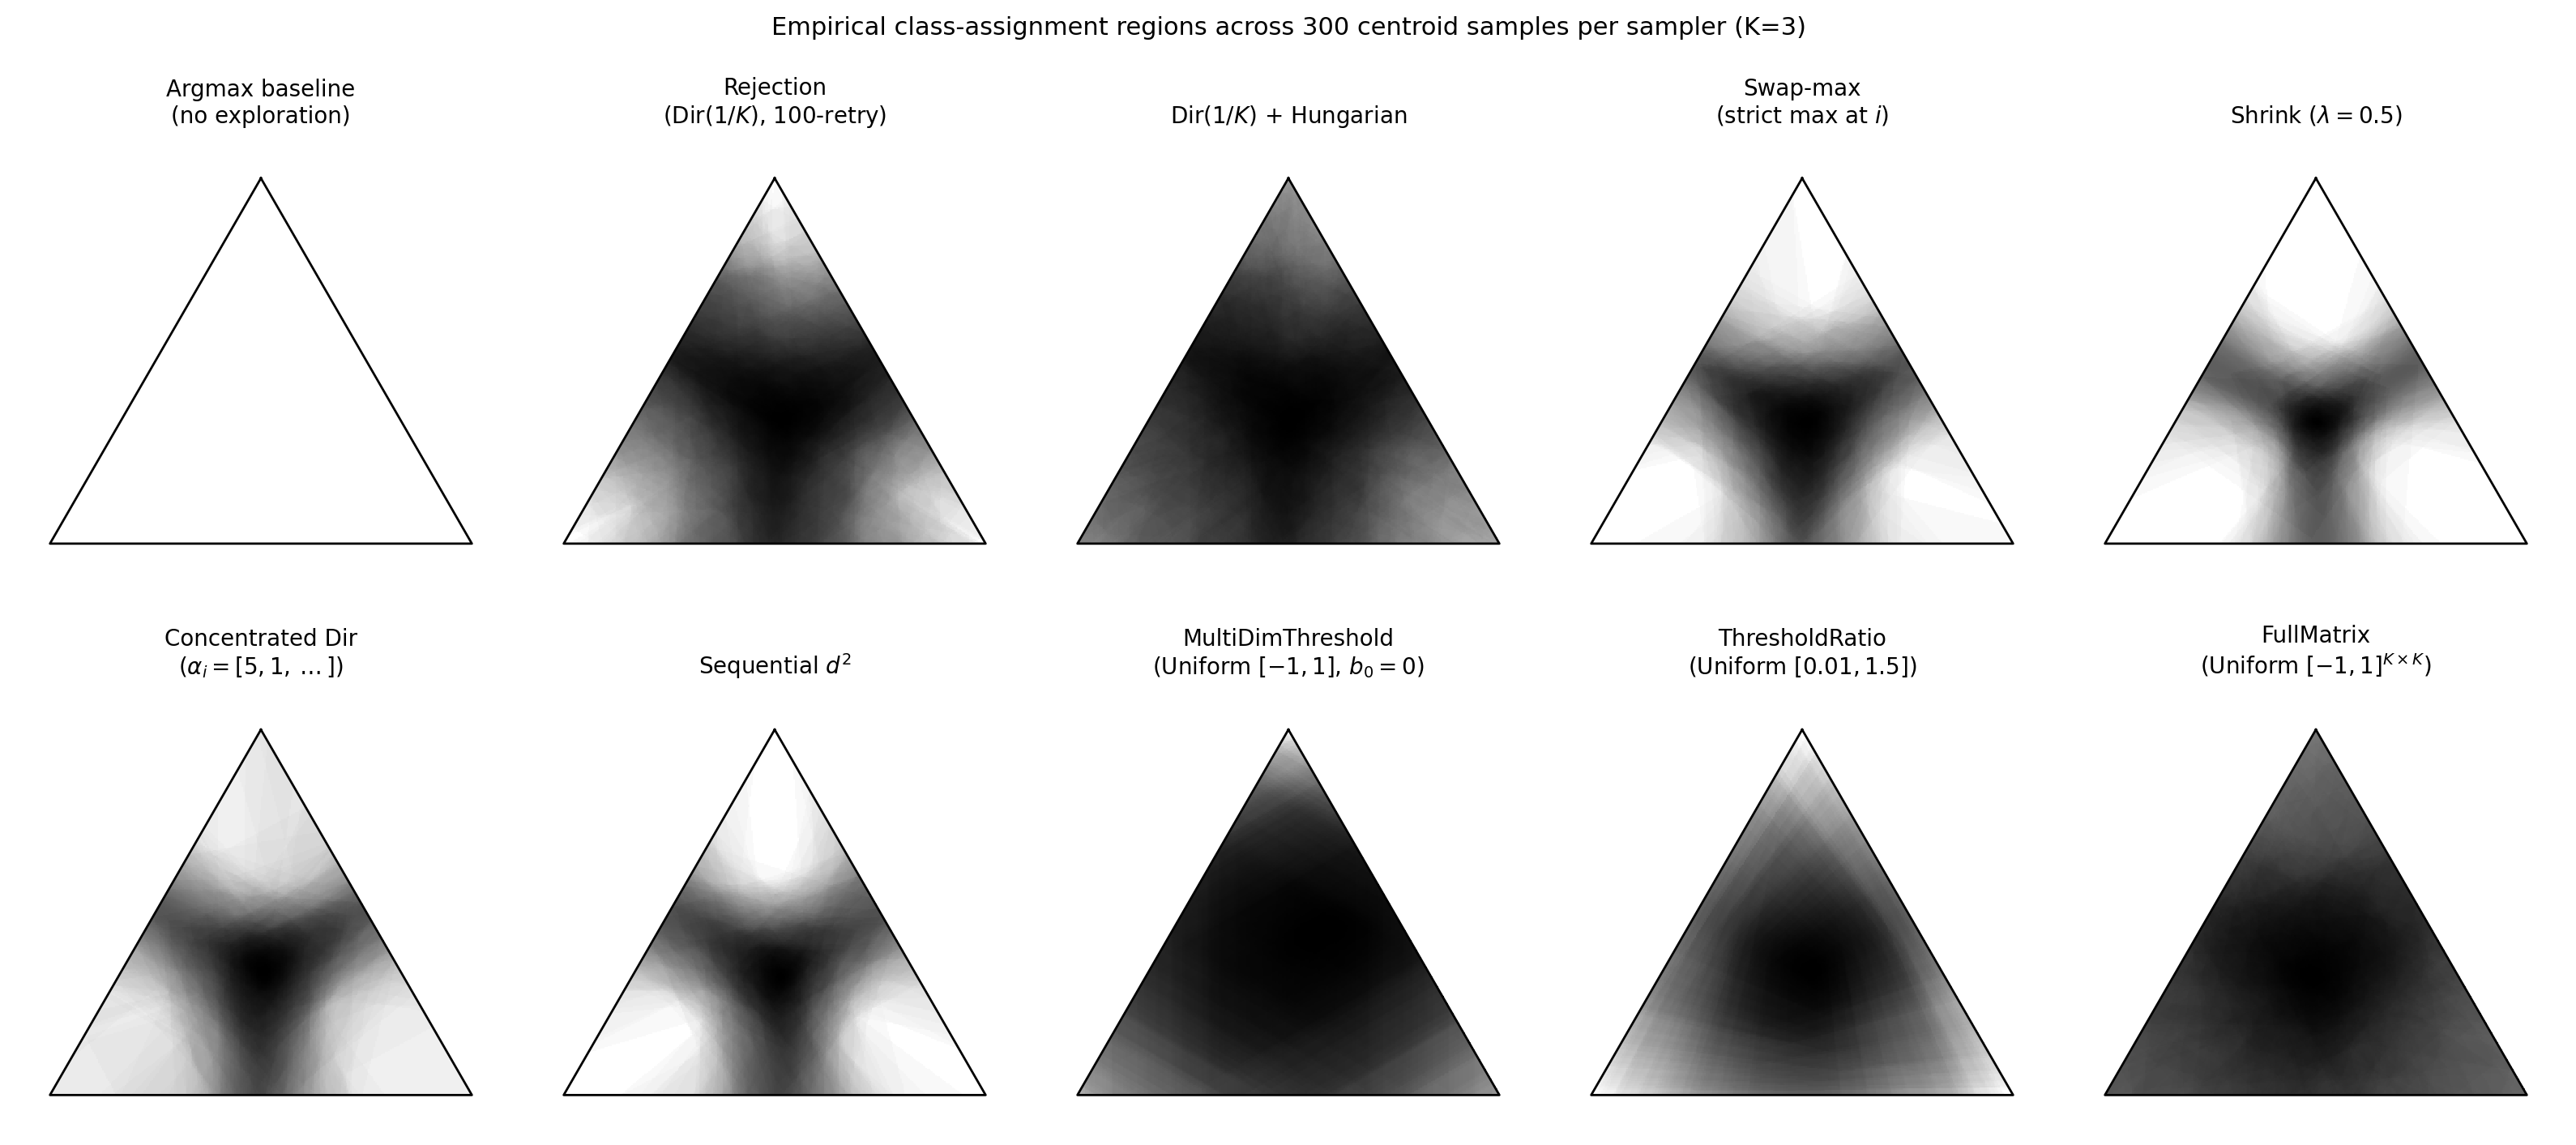
\includegraphics[width=\textwidth]{figures/sampler_partition_overlay.png}
    \caption{Classification disagreement across $300$ sampled configurations per panel at $K=3$. Shade at each grid point is $1 - H(\mathbf{f})$, where $\mathbf{f}$ is the empirical class-fraction vector across samples and $H$ is the Shannon entropy normalised to $[0, 1]$: white marks unanimous agreement on a single class and black marks the uniform distribution over three classes. Rejection and Dir$(1/K)$+Hungarian exhibit dark vertex regions, indicating that the pure-class corners are not consistently decoded to their own class; Shrink keeps the vertex regions white and the interior near-white, reflecting its limited exploration range; Sequential $d^2$ keeps the vertex regions white while producing interior disagreement comparable to Hungarian.}\label{fig:sampler_partition_overlay}
\end{figure}

The rejection baseline and sequential $d^2$ are the two retry-based samplers; Figure~\ref{fig:sampler_rejection_rate} reports their exhaustion rate as a function of $K$ for $M \in \{10, 100, 500\}$. The rejection baseline asymptotes at one for every $M$, confirming that its failure mode is structural in $K$ rather than budget-bounded. Sequential $d^2$ exhausts at zero for $M \geq 100$ across the entire sweep, because the joint acceptance condition~\eqref{eq:seqd2_accept} concentrates the sampler on configurations satisfying the invariant rather than filtering from an uninformative prior.

\begin{figure}[H]
    \centering
    % Auto-generated by experiments.analysis.generate_sampler_overlay_figure --- do not edit.
\resizebox{\textwidth}{!}{%
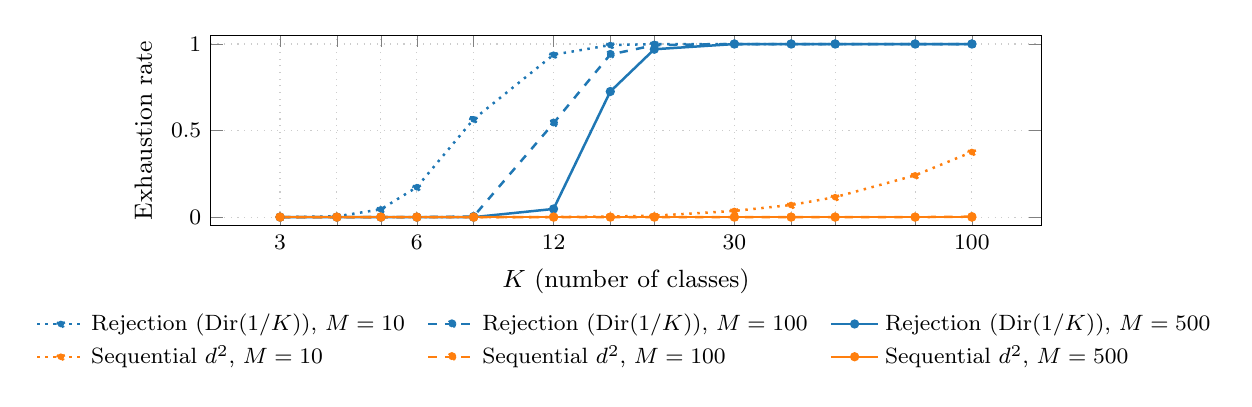
\begin{tikzpicture}
\begin{axis}[
    width=\textwidth, height=4.0cm,
    xlabel={$K$ (number of classes)},
    ylabel={Exhaustion rate},
    xmode=log, log basis x=10, log ticks with fixed point,
    xtick={3,4,5,6,8,12,16,20,30,40,50,75,100},
    xticklabels={3,,,6,,12,,,30,,,,100},
    ymin=-0.05, ymax=1.05,
    grid=major, grid style={dotted, gray!40},
    legend cell align=left,
    legend style={
        at={(0.5,-0.40)}, anchor=north,
        legend columns=3,
        /tikz/every even column/.append style={column sep=0.6em},
        font=\footnotesize, draw=none, fill=none,
    },
    tick label style={font=\footnotesize},
    label style={font=\small},
]
\addplot[
    color={rgb,255:red,31; green,119; blue,180}, mark=*, mark size=1.2pt, line width=0.9pt, dotted,
    error bars/y dir=both, error bars/y explicit,
    error bars/error bar style={line width=0.5pt}
] coordinates {
        (3, 0) +- (0, 0)
        (4, 0.00466667) +- (0, 0.00152853)
        (5, 0.045) +- (0, 0.00629695)
        (6, 0.173) +- (0, 0.0107969)
        (8, 0.565167) +- (0, 0.0141756)
        (12, 0.938333) +- (0, 0.00661025)
        (16, 0.994) +- (0, 0.00187206)
        (20, 0.9995) +- (0, 0.000535196)
        (30, 1) +- (0, 0)
        (40, 1) +- (0, 0)
        (50, 1) +- (0, 0)
        (75, 1) +- (0, 0)
        (100, 1) +- (0, 0)
    };
\addlegendentry{Rejection (Dir$(1/K)$), $M=10$}
\addplot[
    color={rgb,255:red,31; green,119; blue,180}, mark=*, mark size=1.2pt, line width=0.9pt, dashed,
    error bars/y dir=both, error bars/y explicit,
    error bars/error bar style={line width=0.5pt}
] coordinates {
        (3, 0) +- (0, 0)
        (4, 0) +- (0, 0)
        (5, 0) +- (0, 0)
        (6, 0) +- (0, 0)
        (8, 0.00366667) +- (0, 0.00221809)
        (12, 0.542833) +- (0, 0.00978595)
        (16, 0.9395) +- (0, 0.00650361)
        (20, 0.993167) +- (0, 0.00234487)
        (30, 1) +- (0, 0)
        (40, 1) +- (0, 0)
        (50, 1) +- (0, 0)
        (75, 1) +- (0, 0)
        (100, 1) +- (0, 0)
    };
\addlegendentry{Rejection (Dir$(1/K)$), $M=100$}
\addplot[
    color={rgb,255:red,31; green,119; blue,180}, mark=*, mark size=1.2pt, line width=0.9pt, solid,
    error bars/y dir=both, error bars/y explicit,
    error bars/error bar style={line width=0.5pt}
] coordinates {
        (3, 0) +- (0, 0)
        (4, 0) +- (0, 0)
        (5, 0) +- (0, 0)
        (6, 0) +- (0, 0)
        (8, 0) +- (0, 0)
        (12, 0.0473333) +- (0, 0.00520513)
        (16, 0.725667) +- (0, 0.0132638)
        (20, 0.969833) +- (0, 0.00427829)
        (30, 0.999833) +- (0, 0.000326667)
        (40, 1) +- (0, 0)
        (50, 1) +- (0, 0)
        (75, 1) +- (0, 0)
        (100, 1) +- (0, 0)
    };
\addlegendentry{Rejection (Dir$(1/K)$), $M=500$}
\addplot[
    color={rgb,255:red,255; green,127; blue,14}, mark=*, mark size=1.2pt, line width=0.9pt, dotted,
    error bars/y dir=both, error bars/y explicit,
    error bars/error bar style={line width=0.5pt}
] coordinates {
        (3, 0) +- (0, 0)
        (4, 0) +- (0, 0)
        (5, 0) +- (0, 0)
        (6, 0) +- (0, 0)
        (8, 0) +- (0, 0)
        (12, 0.000833333) +- (0, 0.000803668)
        (16, 0.0035) +- (0, 0.00153403)
        (20, 0.00833333) +- (0, 0.00160734)
        (30, 0.0358333) +- (0, 0.0049)
        (40, 0.0701667) +- (0, 0.00537239)
        (50, 0.115333) +- (0, 0.00455611)
        (75, 0.241333) +- (0, 0.0132832)
        (100, 0.376333) +- (0, 0.0108385)
    };
\addlegendentry{Sequential $d^2$, $M=10$}
\addplot[
    color={rgb,255:red,255; green,127; blue,14}, mark=*, mark size=1.2pt, line width=0.9pt, dashed,
    error bars/y dir=both, error bars/y explicit,
    error bars/error bar style={line width=0.5pt}
] coordinates {
        (3, 0) +- (0, 0)
        (4, 0) +- (0, 0)
        (5, 0) +- (0, 0)
        (6, 0) +- (0, 0)
        (8, 0) +- (0, 0)
        (12, 0) +- (0, 0)
        (16, 0) +- (0, 0)
        (20, 0) +- (0, 0)
        (30, 0) +- (0, 0)
        (40, 0.000166667) +- (0, 0.000326667)
        (50, 0.000333333) +- (0, 0.000449655)
        (75, 0.000166667) +- (0, 0.000326667)
        (100, 0.00266667) +- (0, 0.00154316)
    };
\addlegendentry{Sequential $d^2$, $M=100$}
\addplot[
    color={rgb,255:red,255; green,127; blue,14}, mark=*, mark size=1.2pt, line width=0.9pt, solid,
    error bars/y dir=both, error bars/y explicit,
    error bars/error bar style={line width=0.5pt}
] coordinates {
        (3, 0) +- (0, 0)
        (4, 0) +- (0, 0)
        (5, 0) +- (0, 0)
        (6, 0) +- (0, 0)
        (8, 0) +- (0, 0)
        (12, 0) +- (0, 0)
        (16, 0) +- (0, 0)
        (20, 0) +- (0, 0)
        (30, 0) +- (0, 0)
        (40, 0) +- (0, 0)
        (50, 0) +- (0, 0)
        (75, 0) +- (0, 0)
        (100, 0) +- (0, 0)
    };
\addlegendentry{Sequential $d^2$, $M=500$}
\end{axis}
\end{tikzpicture}%
}

    \caption{Exhaustion rate versus $K$ for the two retry-based samplers under three retry budgets $M \in \{10, 100, 500\}$. Colour identifies the sampler (blue: rejection baseline, orange: sequential $d^2$); line style identifies the budget (dotted: $M{=}10$, dashed: $M{=}100$, solid: $M{=}500$). Each marker is the fraction of sampler calls (over $20$ trials of $300$ draws each) that exhausted the budget without producing a valid configuration; error bars are $95\%$ confidence intervals across trials.}\label{fig:sampler_rejection_rate}
\end{figure}

Figure~\ref{fig:sampler_metrics_vs_k} sweeps $K \in \{3, 4, 5, 6, 8, 12, 16, 20, 30, 40, 50, 75, 100\}$ and reports three summary statistics per sampler, averaged over only those draws that did not raise. The left panel is the fraction of successful draws satisfying~\eqref{eq:dlc}; sequential $d^2$, Shrink, argmax, and ThresholdRatio remain at $1.0$ by construction, while Hungarian, Swap-max, Concentrated Dirichlet, MultidimensionalThreshold, and FullMatrix decrease monotonically with $K$. The middle panel is the mean disagreement entropy across a simplex grid (the average greyscale darkness in Figure~\ref{fig:sampler_partition_overlay}), measuring how much independent draws of the same sampler disagree on the same input. The right panel is the partition deviation from argmax: the fraction of grid points whose predicted class differs from $\arg\max_{j \in \mathcal{Y}} p_j$, averaged over successful draws. The two panels separate exploration magnitude (deviation) from exploration variability (entropy): a sampler that consistently produces a partition far from argmax scores high on the right and low in the middle.

\begin{figure}[H]
    \centering
    % Auto-generated by experiments.analysis.generate_sampler_overlay_figure --- do not edit.
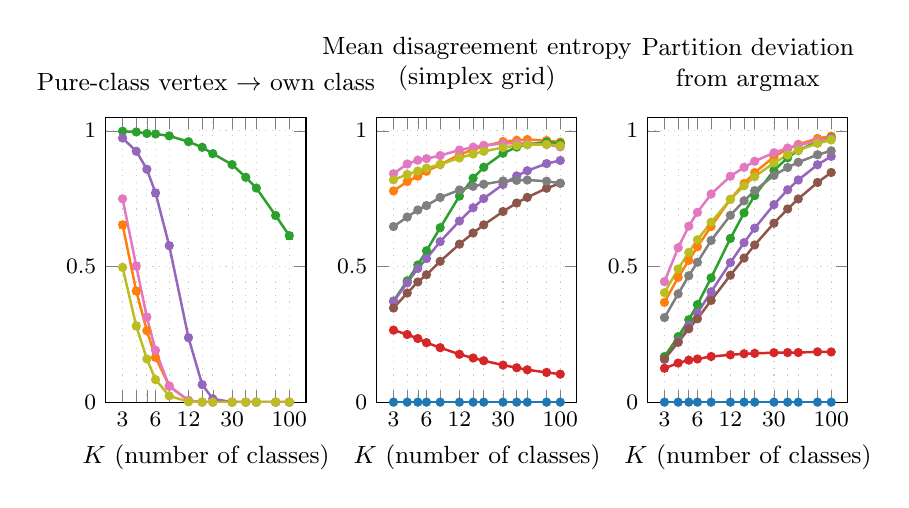
\begin{tikzpicture}
\begin{groupplot}[
    group style={group size=3 by 1, horizontal sep=0.9cm},
    width=0.34\textwidth, height=5.2cm,
    xmode=log, log basis x=10, log ticks with fixed point,
    xtick={3,4,5,6,8,12,16,20,30,40,50,75,100},
    xticklabels={3,,,6,,12,,,30,,,,100},
    ymin=0, ymax=1.05,
    xlabel={$K$ (number of classes)},
    grid=major, grid style={dotted, gray!40},
    tick label style={font=\footnotesize},
    label style={font=\small},
    title style={font=\small, align=center},
]
\nextgroupplot[title={Pure-class vertex $\to$ own class}]
\addplot[
    color={rgb,255:red,255; green,127; blue,14}, mark=*, mark size=1.2pt, line width=0.9pt, solid,
    error bars/y dir=both, error bars/y explicit,
    error bars/error bar style={line width=0.5pt}
] coordinates {
        (3, 0.6535) +- (0, 0.0131051)
        (4, 0.4095) +- (0, 0.0118899)
        (5, 0.263333) +- (0, 0.00895555)
        (6, 0.165) +- (0, 0.00993659)
        (8, 0.0596667) +- (0, 0.00415644)
        (12, 0.006) +- (0, 0.00161431)
        (16, 0.000666667) +- (0, 0.000764266)
        (20, 0) +- (0, 0)
        (30, 0) +- (0, 0)
        (40, 0) +- (0, 0)
        (50, 0) +- (0, 0)
        (75, 0) +- (0, 0)
        (100, 0) +- (0, 0)
    };
\addplot[
    color={rgb,255:red,44; green,160; blue,44}, mark=*, mark size=1.2pt, line width=0.9pt, solid,
    error bars/y dir=both, error bars/y explicit,
    error bars/error bar style={line width=0.5pt}
] coordinates {
        (3, 0.9985) +- (0, 0.00110905)
        (4, 0.995667) +- (0, 0.00117064)
        (5, 0.990167) +- (0, 0.0023923)
        (6, 0.988333) +- (0, 0.00266019)
        (8, 0.981333) +- (0, 0.00269793)
        (12, 0.959833) +- (0, 0.0045084)
        (16, 0.939167) +- (0, 0.00603042)
        (20, 0.915833) +- (0, 0.00896652)
        (30, 0.8755) +- (0, 0.00752827)
        (40, 0.828833) +- (0, 0.0093155)
        (50, 0.789) +- (0, 0.00865058)
        (75, 0.687833) +- (0, 0.00967048)
        (100, 0.613667) +- (0, 0.0129882)
    };
\addplot[
    color={rgb,255:red,148; green,103; blue,189}, mark=*, mark size=1.2pt, line width=0.9pt, solid,
    error bars/y dir=both, error bars/y explicit,
    error bars/error bar style={line width=0.5pt}
] coordinates {
        (3, 0.973333) +- (0, 0.00328381)
        (4, 0.924667) +- (0, 0.00551528)
        (5, 0.858333) +- (0, 0.00692559)
        (6, 0.771) +- (0, 0.0113666)
        (8, 0.576667) +- (0, 0.00970208)
        (12, 0.2375) +- (0, 0.0101311)
        (16, 0.0646667) +- (0, 0.00739466)
        (20, 0.0125) +- (0, 0.00295524)
        (30, 0) +- (0, 0)
        (40, 0) +- (0, 0)
        (50, 0) +- (0, 0)
        (75, 0) +- (0, 0)
        (100, 0) +- (0, 0)
    };
\addplot[
    color={rgb,255:red,227; green,119; blue,194}, mark=*, mark size=1.2pt, line width=0.9pt, solid,
    error bars/y dir=both, error bars/y explicit,
    error bars/error bar style={line width=0.5pt}
] coordinates {
        (3, 0.749333) +- (0, 0.0097782)
        (4, 0.5015) +- (0, 0.0120978)
        (5, 0.313333) +- (0, 0.0140124)
        (6, 0.191333) +- (0, 0.0103453)
        (8, 0.0585) +- (0, 0.00705376)
        (12, 0.00616667) +- (0, 0.00228667)
        (16, 0) +- (0, 0)
        (20, 0) +- (0, 0)
        (30, 0) +- (0, 0)
        (40, 0) +- (0, 0)
        (50, 0) +- (0, 0)
        (75, 0) +- (0, 0)
        (100, 0) +- (0, 0)
    };
\addplot[
    color={rgb,255:red,188; green,189; blue,34}, mark=*, mark size=1.2pt, line width=0.9pt, solid,
    error bars/y dir=both, error bars/y explicit,
    error bars/error bar style={line width=0.5pt}
] coordinates {
        (3, 0.496667) +- (0, 0.00912946)
        (4, 0.2805) +- (0, 0.0110679)
        (5, 0.159167) +- (0, 0.00952536)
        (6, 0.083) +- (0, 0.00560618)
        (8, 0.0233333) +- (0, 0.00373211)
        (12, 0.00133333) +- (0, 0.000873972)
        (16, 0.000333333) +- (0, 0.000653333)
        (20, 0) +- (0, 0)
        (30, 0) +- (0, 0)
        (40, 0) +- (0, 0)
        (50, 0) +- (0, 0)
        (75, 0) +- (0, 0)
        (100, 0) +- (0, 0)
    };
\nextgroupplot[title={Mean disagreement entropy \\ (simplex grid)}]
\addplot[
    color={rgb,255:red,31; green,119; blue,180}, mark=*, mark size=1.2pt, line width=0.9pt, solid,
    error bars/y dir=both, error bars/y explicit,
    error bars/error bar style={line width=0.5pt}
] coordinates {
        (3, 0) +- (0, 0)
        (4, 0) +- (0, 0)
        (5, 0) +- (0, 0)
        (6, 0) +- (0, 0)
        (8, 0) +- (0, 0)
        (12, 0) +- (0, 0)
        (16, 0) +- (0, 0)
        (20, 0) +- (0, 0)
        (30, 0) +- (0, 0)
        (40, 0) +- (0, 0)
        (50, 0) +- (0, 0)
        (75, 0) +- (0, 0)
        (100, 0) +- (0, 0)
    };
\addplot[
    color={rgb,255:red,255; green,127; blue,14}, mark=*, mark size=1.2pt, line width=0.9pt, solid,
    error bars/y dir=both, error bars/y explicit,
    error bars/error bar style={line width=0.5pt}
] coordinates {
        (3, 0.77837) +- (0, 0.00585969)
        (4, 0.813056) +- (0, 0.00472878)
        (5, 0.832734) +- (0, 0.00288057)
        (6, 0.850708) +- (0, 0.00320886)
        (8, 0.875537) +- (0, 0.00223782)
        (12, 0.911993) +- (0, 0.00151792)
        (16, 0.930978) +- (0, 0.00146938)
        (20, 0.943361) +- (0, 0.00129199)
        (30, 0.960389) +- (0, 0.00107288)
        (40, 0.965026) +- (0, 0.000798964)
        (50, 0.967955) +- (0, 0.000908311)
        (75, 0.964269) +- (0, 0.00131859)
        (100, 0.958256) +- (0, 0.00152893)
    };
\addplot[
    color={rgb,255:red,44; green,160; blue,44}, mark=*, mark size=1.2pt, line width=0.9pt, solid,
    error bars/y dir=both, error bars/y explicit,
    error bars/error bar style={line width=0.5pt}
] coordinates {
        (3, 0.372799) +- (0, 0.00593744)
        (4, 0.447166) +- (0, 0.0058969)
        (5, 0.505565) +- (0, 0.00515114)
        (6, 0.557794) +- (0, 0.00371621)
        (8, 0.642779) +- (0, 0.00429098)
        (12, 0.759441) +- (0, 0.00267977)
        (16, 0.825428) +- (0, 0.00347969)
        (20, 0.865639) +- (0, 0.00256653)
        (30, 0.917364) +- (0, 0.0017437)
        (40, 0.940013) +- (0, 0.00130232)
        (50, 0.950407) +- (0, 0.000909989)
        (75, 0.958581) +- (0, 0.00100233)
        (100, 0.953611) +- (0, 0.00225912)
    };
\addplot[
    color={rgb,255:red,214; green,39; blue,40}, mark=*, mark size=1.2pt, line width=0.9pt, solid,
    error bars/y dir=both, error bars/y explicit,
    error bars/error bar style={line width=0.5pt}
] coordinates {
        (3, 0.265537) +- (0, 0.00562947)
        (4, 0.249357) +- (0, 0.00395823)
        (5, 0.234437) +- (0, 0.00394318)
        (6, 0.219159) +- (0, 0.00247256)
        (8, 0.200843) +- (0, 0.00204682)
        (12, 0.176409) +- (0, 0.0024103)
        (16, 0.162717) +- (0, 0.00180198)
        (20, 0.152623) +- (0, 0.0018185)
        (30, 0.136546) +- (0, 0.00158247)
        (40, 0.126753) +- (0, 0.0012205)
        (50, 0.119318) +- (0, 0.00128798)
        (75, 0.109573) +- (0, 0.00092299)
        (100, 0.103191) +- (0, 0.00129697)
    };
\addplot[
    color={rgb,255:red,148; green,103; blue,189}, mark=*, mark size=1.2pt, line width=0.9pt, solid,
    error bars/y dir=both, error bars/y explicit,
    error bars/error bar style={line width=0.5pt}
] coordinates {
        (3, 0.371256) +- (0, 0.00625153)
        (4, 0.439725) +- (0, 0.00531927)
        (5, 0.492492) +- (0, 0.00617642)
        (6, 0.52919) +- (0, 0.00539672)
        (8, 0.591514) +- (0, 0.0035765)
        (12, 0.667666) +- (0, 0.00294207)
        (16, 0.716458) +- (0, 0.00339461)
        (20, 0.750384) +- (0, 0.00194903)
        (30, 0.802315) +- (0, 0.00150149)
        (40, 0.833899) +- (0, 0.000708931)
        (50, 0.852921) +- (0, 0.00119884)
        (75, 0.879233) +- (0, 0.000730223)
        (100, 0.890571) +- (0, 0.000618399)
    };
\addplot[
    color={rgb,255:red,140; green,86; blue,75}, mark=*, mark size=1.2pt, line width=0.9pt, solid,
    error bars/y dir=both, error bars/y explicit,
    error bars/error bar style={line width=0.5pt}
] coordinates {
        (3, 0.346799) +- (0, 0.00527885)
        (4, 0.402057) +- (0, 0.00569766)
        (5, 0.442914) +- (0, 0.00517294)
        (6, 0.469562) +- (0, 0.00338183)
        (8, 0.519007) +- (0, 0.0024014)
        (12, 0.582268) +- (0, 0.00253397)
        (16, 0.623343) +- (0, 0.00242087)
        (20, 0.653314) +- (0, 0.00204929)
        (30, 0.702519) +- (0, 0.00170069)
        (40, 0.733939) +- (0, 0.000966374)
        (50, 0.754689) +- (0, 0.00146493)
        (75, 0.788332) +- (0, 0.00110195)
        (100, 0.806591) +- (0, 0.00073574)
    };
\addplot[
    color={rgb,255:red,227; green,119; blue,194}, mark=*, mark size=1.2pt, line width=0.9pt, solid,
    error bars/y dir=both, error bars/y explicit,
    error bars/error bar style={line width=0.5pt}
] coordinates {
        (3, 0.841806) +- (0, 0.00380629)
        (4, 0.87784) +- (0, 0.00364437)
        (5, 0.891622) +- (0, 0.00362347)
        (6, 0.897392) +- (0, 0.00364769)
        (8, 0.908875) +- (0, 0.00318785)
        (12, 0.92922) +- (0, 0.00180897)
        (16, 0.939459) +- (0, 0.00157958)
        (20, 0.946445) +- (0, 0.0017324)
        (30, 0.95289) +- (0, 0.00122959)
        (40, 0.954904) +- (0, 0.000964237)
        (50, 0.952766) +- (0, 0.00135665)
        (75, 0.949451) +- (0, 0.00177961)
        (100, 0.940819) +- (0, 0.00245238)
    };
\addplot[
    color={rgb,255:red,127; green,127; blue,127}, mark=*, mark size=1.2pt, line width=0.9pt, solid,
    error bars/y dir=both, error bars/y explicit,
    error bars/error bar style={line width=0.5pt}
] coordinates {
        (3, 0.647221) +- (0, 0.0075065)
        (4, 0.682117) +- (0, 0.00784401)
        (5, 0.708197) +- (0, 0.00661577)
        (6, 0.724471) +- (0, 0.00531476)
        (8, 0.754369) +- (0, 0.00480233)
        (12, 0.782009) +- (0, 0.0032986)
        (16, 0.795448) +- (0, 0.00299954)
        (20, 0.803172) +- (0, 0.00265332)
        (30, 0.815186) +- (0, 0.00308205)
        (40, 0.817452) +- (0, 0.00249688)
        (50, 0.818564) +- (0, 0.00210879)
        (75, 0.814271) +- (0, 0.00161582)
        (100, 0.80669) +- (0, 0.00105788)
    };
\addplot[
    color={rgb,255:red,188; green,189; blue,34}, mark=*, mark size=1.2pt, line width=0.9pt, solid,
    error bars/y dir=both, error bars/y explicit,
    error bars/error bar style={line width=0.5pt}
] coordinates {
        (3, 0.819566) +- (0, 0.00501197)
        (4, 0.839068) +- (0, 0.0056958)
        (5, 0.851929) +- (0, 0.00361308)
        (6, 0.862499) +- (0, 0.00290218)
        (8, 0.876193) +- (0, 0.00210679)
        (12, 0.900123) +- (0, 0.00108741)
        (16, 0.914479) +- (0, 0.000905028)
        (20, 0.924322) +- (0, 0.000887098)
        (30, 0.93831) +- (0, 0.000581018)
        (40, 0.945657) +- (0, 0.000512726)
        (50, 0.948428) +- (0, 0.000379355)
        (75, 0.949459) +- (0, 0.000388088)
        (100, 0.945453) +- (0, 0.000252369)
    };
\nextgroupplot[title={Partition deviation \\ from argmax},
    legend to name=samplerlegendmetrics,
    legend style={
        font=\footnotesize, draw=none, fill=none,
        legend columns=4,
        /tikz/every even column/.append style={column sep=0.6em},
    },
    legend cell align=left]
\addplot[
    color={rgb,255:red,31; green,119; blue,180}, mark=*, mark size=1.2pt, line width=0.9pt, solid,
    error bars/y dir=both, error bars/y explicit,
    error bars/error bar style={line width=0.5pt}
] coordinates {
        (3, 0) +- (0, 0)
        (4, 0) +- (0, 0)
        (5, 0) +- (0, 0)
        (6, 0) +- (0, 0)
        (8, 0) +- (0, 0)
        (12, 0) +- (0, 0)
        (16, 0) +- (0, 0)
        (20, 0) +- (0, 0)
        (30, 0) +- (0, 0)
        (40, 0) +- (0, 0)
        (50, 0) +- (0, 0)
        (75, 0) +- (0, 0)
        (100, 0) +- (0, 0)
    };
\addplot[
    color={rgb,255:red,255; green,127; blue,14}, mark=*, mark size=1.2pt, line width=0.9pt, solid,
    error bars/y dir=both, error bars/y explicit,
    error bars/error bar style={line width=0.5pt}
] coordinates {
        (3, 0.367732) +- (0, 0.0043432)
        (4, 0.459895) +- (0, 0.00434397)
        (5, 0.522282) +- (0, 0.00288499)
        (6, 0.572665) +- (0, 0.00350981)
        (8, 0.647334) +- (0, 0.00269877)
        (12, 0.747536) +- (0, 0.00188312)
        (16, 0.805781) +- (0, 0.00187474)
        (20, 0.84587) +- (0, 0.00156137)
        (30, 0.904187) +- (0, 0.000748952)
        (40, 0.933224) +- (0, 0.000728659)
        (50, 0.950068) +- (0, 0.000569008)
        (75, 0.971754) +- (0, 0.00043202)
        (100, 0.980786) +- (0, 0.000229619)
    };
\addplot[
    color={rgb,255:red,44; green,160; blue,44}, mark=*, mark size=1.2pt, line width=0.9pt, solid,
    error bars/y dir=both, error bars/y explicit,
    error bars/error bar style={line width=0.5pt}
] coordinates {
        (3, 0.168111) +- (0, 0.00338015)
        (4, 0.241462) +- (0, 0.00362543)
        (5, 0.30383) +- (0, 0.00350984)
        (6, 0.359529) +- (0, 0.00300043)
        (8, 0.458015) +- (0, 0.00336196)
        (12, 0.603403) +- (0, 0.00249757)
        (16, 0.697615) +- (0, 0.00320266)
        (20, 0.761199) +- (0, 0.00256102)
        (30, 0.85422) +- (0, 0.00145083)
        (40, 0.900721) +- (0, 0.00115666)
        (50, 0.927489) +- (0, 0.00105105)
        (75, 0.960694) +- (0, 0.000699423)
        (100, 0.974178) +- (0, 0.000359782)
    };
\addplot[
    color={rgb,255:red,214; green,39; blue,40}, mark=*, mark size=1.2pt, line width=0.9pt, solid,
    error bars/y dir=both, error bars/y explicit,
    error bars/error bar style={line width=0.5pt}
] coordinates {
        (3, 0.124882) +- (0, 0.00261134)
        (4, 0.144149) +- (0, 0.00246368)
        (5, 0.154808) +- (0, 0.00286235)
        (6, 0.159126) +- (0, 0.00213982)
        (8, 0.168398) +- (0, 0.00231317)
        (12, 0.174299) +- (0, 0.00289588)
        (16, 0.178388) +- (0, 0.00243734)
        (20, 0.179814) +- (0, 0.0026394)
        (30, 0.182278) +- (0, 0.00290332)
        (40, 0.182722) +- (0, 0.00223039)
        (50, 0.182901) +- (0, 0.00257952)
        (75, 0.185486) +- (0, 0.00150741)
        (100, 0.185081) +- (0, 0.00256207)
    };
\addplot[
    color={rgb,255:red,148; green,103; blue,189}, mark=*, mark size=1.2pt, line width=0.9pt, solid,
    error bars/y dir=both, error bars/y explicit,
    error bars/error bar style={line width=0.5pt}
] coordinates {
        (3, 0.157405) +- (0, 0.00303679)
        (4, 0.225645) +- (0, 0.0033817)
        (5, 0.283244) +- (0, 0.00409966)
        (6, 0.328151) +- (0, 0.00355737)
        (8, 0.406721) +- (0, 0.00267064)
        (12, 0.514332) +- (0, 0.00288974)
        (16, 0.587824) +- (0, 0.00310824)
        (20, 0.641093) +- (0, 0.00205485)
        (30, 0.728017) +- (0, 0.00168531)
        (40, 0.782648) +- (0, 0.000894158)
        (50, 0.818767) +- (0, 0.00140421)
        (75, 0.874868) +- (0, 0.000998815)
        (100, 0.905719) +- (0, 0.000880204)
    };
\addplot[
    color={rgb,255:red,140; green,86; blue,75}, mark=*, mark size=1.2pt, line width=0.9pt, solid,
    error bars/y dir=both, error bars/y explicit,
    error bars/error bar style={line width=0.5pt}
] coordinates {
        (3, 0.159691) +- (0, 0.00284143)
        (4, 0.220365) +- (0, 0.00332963)
        (5, 0.270407) +- (0, 0.00367207)
        (6, 0.307172) +- (0, 0.0027213)
        (8, 0.374889) +- (0, 0.00201705)
        (12, 0.46779) +- (0, 0.0024261)
        (16, 0.531006) +- (0, 0.00238303)
        (20, 0.579214) +- (0, 0.00235585)
        (30, 0.659605) +- (0, 0.00190598)
        (40, 0.711961) +- (0, 0.00126868)
        (50, 0.748901) +- (0, 0.00185437)
        (75, 0.80954) +- (0, 0.00137474)
        (100, 0.846412) +- (0, 0.00126185)
    };
\addplot[
    color={rgb,255:red,227; green,119; blue,194}, mark=*, mark size=1.2pt, line width=0.9pt, solid,
    error bars/y dir=both, error bars/y explicit,
    error bars/error bar style={line width=0.5pt}
] coordinates {
        (3, 0.444159) +- (0, 0.00374994)
        (4, 0.568977) +- (0, 0.00395233)
        (5, 0.64859) +- (0, 0.00420293)
        (6, 0.699492) +- (0, 0.00383452)
        (8, 0.766746) +- (0, 0.00246998)
        (12, 0.832669) +- (0, 0.00245901)
        (16, 0.865284) +- (0, 0.00168187)
        (20, 0.887737) +- (0, 0.0011488)
        (30, 0.919201) +- (0, 0.000942476)
        (40, 0.936399) +- (0, 0.00060299)
        (50, 0.946984) +- (0, 0.000466637)
        (75, 0.962395) +- (0, 0.000427416)
        (100, 0.970486) +- (0, 0.000354685)
    };
\addplot[
    color={rgb,255:red,127; green,127; blue,127}, mark=*, mark size=1.2pt, line width=0.9pt, solid,
    error bars/y dir=both, error bars/y explicit,
    error bars/error bar style={line width=0.5pt}
] coordinates {
        (3, 0.311681) +- (0, 0.00548634)
        (4, 0.399075) +- (0, 0.00606963)
        (5, 0.465765) +- (0, 0.00605427)
        (6, 0.51548) +- (0, 0.00487938)
        (8, 0.595761) +- (0, 0.00409933)
        (12, 0.688682) +- (0, 0.00325143)
        (16, 0.742075) +- (0, 0.00232123)
        (20, 0.779371) +- (0, 0.00210046)
        (30, 0.835683) +- (0, 0.00189765)
        (40, 0.864892) +- (0, 0.0014669)
        (50, 0.884106) +- (0, 0.00128854)
        (75, 0.911753) +- (0, 0.000918897)
        (100, 0.926173) +- (0, 0.000655623)
    };
\addplot[
    color={rgb,255:red,188; green,189; blue,34}, mark=*, mark size=1.2pt, line width=0.9pt, solid,
    error bars/y dir=both, error bars/y explicit,
    error bars/error bar style={line width=0.5pt}
] coordinates {
        (3, 0.403405) +- (0, 0.00445641)
        (4, 0.490825) +- (0, 0.00499481)
        (5, 0.552072) +- (0, 0.00343839)
        (6, 0.59841) +- (0, 0.00299632)
        (8, 0.662986) +- (0, 0.00232583)
        (12, 0.747383) +- (0, 0.00135307)
        (16, 0.797368) +- (0, 0.000940028)
        (20, 0.831009) +- (0, 0.000968433)
        (30, 0.8819) +- (0, 0.000462139)
        (40, 0.910841) +- (0, 0.000558771)
        (50, 0.928291) +- (0, 0.000424632)
        (75, 0.953425) +- (0, 0.000316544)
        (100, 0.96624) +- (0, 0.000197039)
    };
\addlegendimage{color={rgb,255:red,31; green,119; blue,180}, mark=*, mark size=1.2pt, line width=0.9pt}
\addlegendentry{Argmax}
\addlegendimage{color={rgb,255:red,255; green,127; blue,14}, mark=*, mark size=1.2pt, line width=0.9pt}
\addlegendentry{Hungarian (Dir$(1/K)$)}
\addlegendimage{color={rgb,255:red,44; green,160; blue,44}, mark=*, mark size=1.2pt, line width=0.9pt}
\addlegendentry{Swap-max}
\addlegendimage{color={rgb,255:red,214; green,39; blue,40}, mark=*, mark size=1.2pt, line width=0.9pt}
\addlegendentry{Shrink ($\lambda=0.5$)}
\addlegendimage{color={rgb,255:red,148; green,103; blue,189}, mark=*, mark size=1.2pt, line width=0.9pt}
\addlegendentry{Concentrated Dir}
\addlegendimage{color={rgb,255:red,140; green,86; blue,75}, mark=*, mark size=1.2pt, line width=0.9pt}
\addlegendentry{Sequential $d^2$}
\addlegendimage{color={rgb,255:red,227; green,119; blue,194}, mark=*, mark size=1.2pt, line width=0.9pt}
\addlegendentry{MultiDimThreshold}
\addlegendimage{color={rgb,255:red,127; green,127; blue,127}, mark=*, mark size=1.2pt, line width=0.9pt}
\addlegendentry{ThresholdRatio}
\addlegendimage{color={rgb,255:red,188; green,189; blue,34}, mark=*, mark size=1.2pt, line width=0.9pt}
\addlegendentry{FullMatrix}
\end{groupplot}
\end{tikzpicture}%
\par\smallskip
\centerline{\ref{samplerlegendmetrics}}

    \caption{Sampler metrics as a function of $K$. Markers denote the mean over $20$ independent trials of $300$ sampled configurations; error bars are $95\%$ confidence intervals across trials. All metrics are averaged only over draws that did not raise during construction. Left: fraction of successful draws satisfying $\arg\min_{j \in \mathcal{Y}}\|\mathbf{e}_k-\boldsymbol{\mu}_j\|_2 = \{k\}$ for every $k$. Middle: mean over a simplex grid of the normalised Shannon entropy of the empirical class-fraction vector across samples (the grid-average of the greyscale darkness in Figure~\ref{fig:sampler_partition_overlay}). Right: mean over successful draws of the fraction of grid points classified differently from $\arg\max_{j \in \mathcal{Y}} p_j$.}\label{fig:sampler_metrics_vs_k}
\end{figure}

Among the six Voronoi samplers compared, sequential $d^2$ is the only one that satisfies~\eqref{eq:dlc} with probability one across the entire sweep while producing a partition-deviation footprint comparable to Hungarian; it is therefore the sampler we adopt for the Voronoi optimizer. Shrink also satisfies~\eqref{eq:dlc}, but its reachable configurations stay near the argmax tessellation, so its partition-deviation footprint is small.

Swap-max and Concentrated Dirichlet enforce only a per-centroid marginal of~\eqref{eq:dlc}, not the joint condition across centroids, which is why the left panel of Figure~\ref{fig:sampler_metrics_vs_k} shows their satisfaction fraction decaying as $K$ grows. For swap-max the decay is exact: applying~\eqref{eq:dsq_identity} to~\eqref{eq:dlc}, the constraint is equivalent to
\begin{equation}
    \|\boldsymbol{\mu}_k\|_2^2 - 2\,\boldsymbol{\mu}_k[k] \;<\; \|\boldsymbol{\mu}_j\|_2^2 - 2\,\boldsymbol{\mu}_j[k] \qquad \text{for all } j \neq k,
    \label{eq:voronoi_invariant_expanded}
\end{equation}
which involves the off-diagonal entries $\boldsymbol{\mu}_j[k]$ and the squared norms $\|\boldsymbol{\mu}_j\|_2^2$ that swap-max leaves uncontrolled, so it cannot hold~\eqref{eq:voronoi_invariant_expanded} as $K$ grows, consistent with the observed decay; Concentrated Dirichlet's per-centroid marginal bias breaks~\eqref{eq:dlc} for the same reason.

A broader observation cuts against the Voronoi family as a whole: the two vector-tuned baselines, MultidimensionalThreshold ($\mathcal{H}_{PS}$) and ThresholdRatio ($\mathcal{H}_{Sc}$), achieve sampling-variety metrics competitive with sequential $d^2$ (and in the middle panel of Figure~\ref{fig:sampler_metrics_vs_k}, MultidimensionalThreshold attains the highest disagreement entropy across the entire sweep) without needing any invariant-preserving construction. FullMatrix, the unconstrained $K^2$-parameter family, behaves the same way: it reaches a comparable partition-deviation footprint at zero exhaustion, having no diagonal-dominance invariant to preserve. The DLC machinery of this section is therefore the price of the strictly richer $\mathcal{H}_{Vor}$; staying within $\mathcal{H}_{PS}$ removes the sampling problem entirely.

With sequential $d^2$ as the chosen sampler, Algorithm~\ref{alg:voronoi_tuning} wraps it in an outer random-search loop: initialize at the argmax prototypes, propose a new configuration each iteration, and keep it when it improves the validation score.

\begin{algorithm}[H]
\caption{Voronoi Tuning via Sequential $d^2$ Sampling}\label{alg:voronoi_tuning}
\begin{algorithmic}[1]
\State \textbf{Input:} Validation set $\mathcal{V}=\{(x_i, y_i)\}_{i=1}^m$ with pre-computed scores $\hat{\mathbf{p}}(x_i)$, optimization objective, iterations $T$, retry budget $M$.
\State \textbf{Initialize:} $\mathcal{M}^* \leftarrow \{\mathbf{e}_0, \dots, \mathbf{e}_{K-1}\}$ (standard argmax prototypes).
\State \textbf{Compute baseline score:} $S^* \leftarrow \text{Score}(\mathcal{M}^*, \mathcal{V})$.
\For{$t = 1$ to $T$}
    \State \textit{Sampling step (sequential $d^2$):}
    \For{$i = 0$ to $K-1$}
        \State \textit{attempts} $\leftarrow 0$
        \Repeat
            \State Draw $\mathbf{p} \sim \mathrm{Dir}(\mathbf{1}_K)$; permute coordinates so that $\arg\max_{j \in \mathcal{Y}} p_j = i$.
            \State \textit{attempts} $\leftarrow$ \textit{attempts} $+\,1$
        \Until{for every $k < i$, $d^2(\mathbf{e}_k, \mathbf{p}) > d^2(\mathbf{e}_k, \boldsymbol{\mu}_k)$ and $d^2(\mathbf{e}_i, \mathbf{p}) < d^2(\mathbf{e}_i, \boldsymbol{\mu}_k)$ (condition~\eqref{eq:seqd2_accept}), or \textit{attempts} $= M$}
        \If{\textit{attempts} $= M$ and $\mathbf{p}$ was not accepted}
            \State \textbf{error} ``retry budget $M$ exhausted''
        \EndIf
        \State $\boldsymbol{\mu}_i \leftarrow \mathbf{p}$.
    \EndFor
    \State Let $\mathcal{M}' = \{\boldsymbol{\mu}_0, \ldots, \boldsymbol{\mu}_{K-1}\}$ and compute $\hat{S} \leftarrow \text{Score}(\mathcal{M}', \mathcal{V})$.
    \If{$\hat{S} > S^*$}
        \State $\mathcal{M}^* \leftarrow \mathcal{M}'$, \quad $S^* \leftarrow \hat{S}$.
    \EndIf
\EndFor
\State \textbf{Return} $\mathcal{M}^*$.
\end{algorithmic}
\end{algorithm}

The production implementation sets the retry budget to $M = 500$ as headroom, well above the regime in which Figure~\ref{fig:sampler_rejection_rate} shows the exhaustion rate already vanishing for sequential $d^2$.

\section{A boundary-rotation scenario}\label{sec:boundary_rotation_experiment}

Proposition~\ref{prop:ps_in_vor} states an expressivity inclusion: the best rule in $\mathcal{H}_{Vor}$ has population risk no higher than the best rule in $\mathcal{H}_{PS}$. It does not say when the gap is strict, how large it is, or what survives finite-sample tuning. This section exhibits one regime where the population gap is strict and recoverable.

The mechanism. When the true class-conditional covariances $\Sigma_k$ differ across classes but the probability estimator does not model per-class second-order structure, the Bayes-optimal boundary between classes $i$ and $j$ picks up a quadratic term $\propto \mathbf{x}^\top (\Sigma_i^{-1} - \Sigma_j^{-1})\, \mathbf{x}$ that rotates the pairwise boundary in a direction that depends on $(i, j)$. Parallel shifts ($\mathcal{H}_{PS}$) cannot rotate boundaries at all. Column scaling ($\mathcal{H}_{Sc}$) does rotate the pairwise normals (Proposition~\ref{prop:column_rotation}), but with only $K-1$ free parameters its rotations are coupled across all $\binom{K}{2}$ pairs and need not match the per-pair quadratic. The Voronoi class has $K(K-1)$ parameters and places each pairwise normal as $\boldsymbol{\mu}_j - \boldsymbol{\mu}_i$, the full-matrix class has $K^2$ parameters; both can match the per-pair rotation that $(\Sigma_i^{-1} - \Sigma_j^{-1})$ induces.

The construction. Three Gaussian classes live in $\mathbb{R}^3$ with means
\begin{equation*}
    \boldsymbol{\mu}_0 = (0, 0, 0), \quad \boldsymbol{\mu}_1 = (2, 0, 0), \quad \boldsymbol{\mu}_2 = (1, 2, 0)
\end{equation*}
placed close enough to overlap, and priors $\boldsymbol{\pi} \approx (10, 2, 1)/13$. Every class has unit per-feature variances, but the off-diagonal correlation $\rho = 0.8$ sits in a different coordinate plane in each class:
\begin{equation*}
    \Sigma_0 = \begin{pmatrix} 1 & 0.8 & 0 \\ 0.8 & 1 & 0 \\ 0 & 0 & 1 \end{pmatrix}, \quad
    \Sigma_1 = \begin{pmatrix} 1 & -0.8 & 0 \\ -0.8 & 1 & 0 \\ 0 & 0 & 1 \end{pmatrix}, \quad
    \Sigma_2 = \begin{pmatrix} 1 & 0 & 0.8 \\ 0 & 1 & 0 \\ 0.8 & 0 & 1 \end{pmatrix}.
\end{equation*}
A Gaussian Naive Bayes estimator fitted on the training sample assumes a diagonal covariance and so discards all of this correlation structure; its misspecified probability estimates $\hat{\mathbf{p}}(\mathbf{x}) \in \Delta^{2}$ are what the decision rules operate on. The two objectives are Accuracy and Macro-F1, both symmetric and with no cost matrix.

Under symmetric objectives the structured tuning strategies of Section~\ref{sec:partition_optimization} reduce to two equivalence classes of decision rule: the parallel-shift class $\mathcal{H}_{PS}$ (Eq.~\ref{eq:hps_def}) and the column-scaling class $\mathcal{H}_{Sc}$ (Eq.~\ref{eq:hsc_def}), which is distinct from $\mathcal{H}_{PS}$ in that it rotates the boundary normals (Proposition~\ref{prop:column_rotation}). The comparison uses five strategies: a cost-blind baseline, one representative of each vector-tuned class, the Voronoi prototype family, and the unconstrained partition matrix. RiskPartitioning and LinearScaling would duplicate MultidimensionalThreshold and ThresholdRatio respectively under symmetric objectives, while SequentialSelection's non-convex, order-dependent regions probe a different geometry; the three are omitted.

The five strategies are: Default, the cost-blind $\arg\max_{k \in \mathcal{Y}} p_k$; ThresholdRatio, the probability-ratio rule $\arg\max_{k \in \mathcal{Y}} (\hat{p}_k / \tau_k)$ of Section~\ref{sec:prob_ratio_thresholding}, the $\mathcal{H}_{Sc}$ representative (equivalent under $0/1$ loss to O'Brien's linear class scaling by Proposition~\ref{prop:ratio_equivalence}); MultidimensionalThreshold, the per-class additive bias rule $\arg\max_{k \in \mathcal{Y}} (\hat{p}_k - b_k)$ of \citet{marchetti2025multidimensional} (Section~\ref{sec:multidim_thresholding}), the $\mathcal{H}_{PS}$ representative (equivalent under $0/1$ loss to O'Brien's parallel-shift rule by Proposition~\ref{prop:marchetti_equivalence}); VoronoiTuning, the prototype rule $\arg\min_{k \in \mathcal{Y}} \|\mathbf{p} - \boldsymbol{\mu}_k\|_2$ of Equation~\eqref{eq:voronoi_rule} fit by Algorithm~\ref{alg:voronoi_tuning}, the rotating prototype class at parameter budget $K(K-1)$; and FullMatrixPartitioning, the unconstrained partition rule $\arg\min_{i \in \mathcal{Y}} \mathbf{a}_i^\top \mathbf{p}$ (Eq.~\ref{eq:obrien_rule}) with all $K^2$ entries of $\mathbf{A}$ free, which rotates boundaries unconstrainedly and isolates whether the gap is closed by rotation in general or by the Voronoi parameterization in particular. Full parameterizations, search ranges, warm-starts, and per-strategy sampler settings are deferred to the OpenML campaign of Section~\ref{sec:multiclass_strategies}.

Each tuned strategy is fit by random search ($301$ iterations) on a held-out validation sample against each objective and evaluated on an independent test sample; sample sizes are $6{,}000$ (train), $3{,}000$ (validation), and $10{,}000$ (test), with results averaged over $10$ seeds.

\begin{figure}[H]
    \centering
    \resizebox{\textwidth}{!}{\documentclass[tikz, border=10pt]{standalone}
\usepackage{tikz}
\usepackage{amsmath}
\usetikzlibrary{shapes, calc, backgrounds, arrows.meta}

\begin{document}
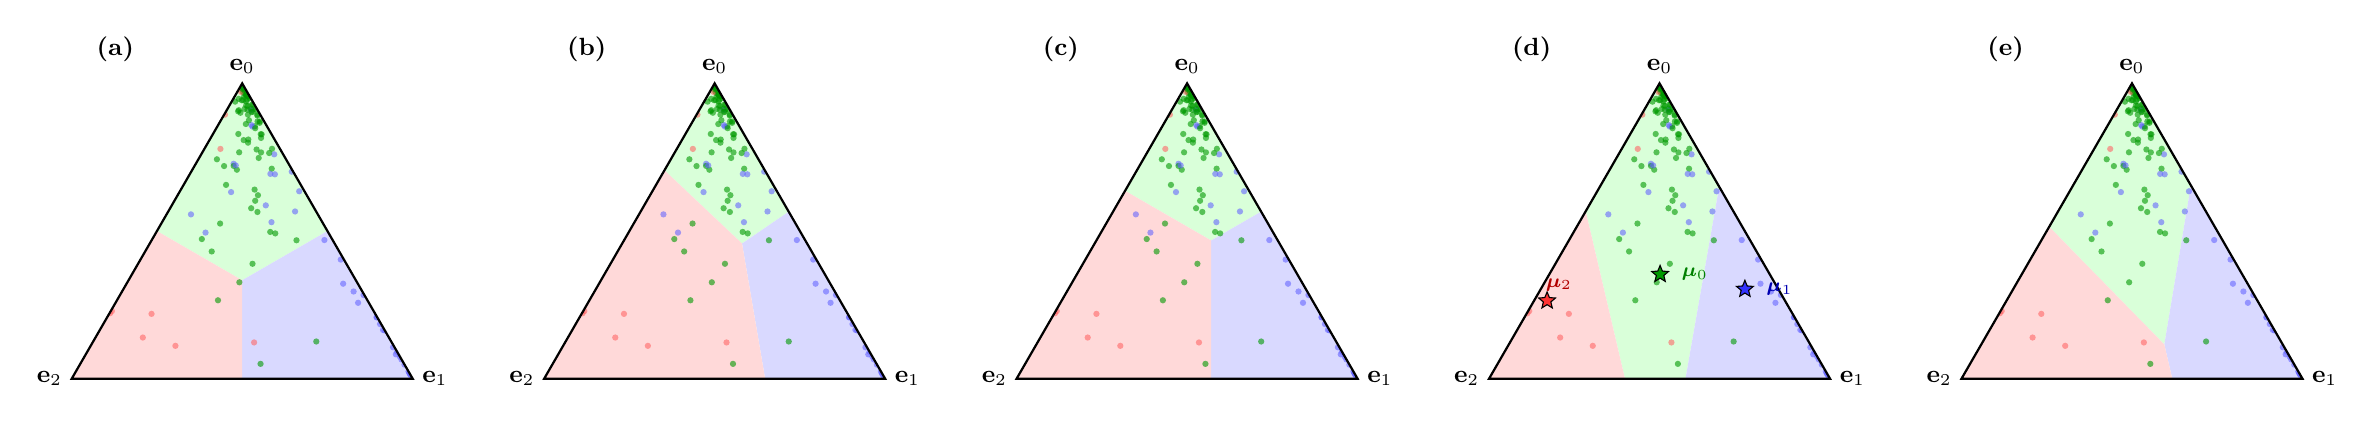
\begin{tikzpicture}[font=\sffamily]

    \begin{scope}[xshift=0.0cm, scale=0.5]
    \coordinate (Top) at (0.000, 5.000);
    \coordinate (Right) at (4.330, -2.500);
    \coordinate (Left) at (-4.330, -2.500);

    \coordinate (Int) at (0.000, 0.000);

    \fill[green!15] (0.000, 5.000) -- (2.165, 1.250) -- (0.000, 0.000) -- (-2.165, 1.250) -- cycle;
    \fill[blue!15] (4.330, -2.500) -- (0.000, -2.500) -- (0.000, 0.000) -- (2.165, 1.250) -- cycle;
    \fill[red!15] (-4.330, -2.500) -- (-2.165, 1.250) -- (0.000, 0.000) -- (0.000, -2.500) -- cycle;

    \begin{scope}
        \clip (Top) -- (Right) -- (Left) -- cycle;

    % --- Data points ---
    \node[circle, fill=red!60, fill opacity=0.6, inner sep=0.8pt, draw=none] at (-3.310, -0.782) {};
    \node[circle, fill=green!60!black, fill opacity=0.6, inner sep=0.8pt, draw=none] at (0.757, 3.339) {};
    \node[circle, fill=green!60!black, fill opacity=0.6, inner sep=0.8pt, draw=none] at (-0.460, 2.900) {};
    \node[circle, fill=green!60!black, fill opacity=0.6, inner sep=0.8pt, draw=none] at (0.070, 4.862) {};
    \node[circle, fill=green!60!black, fill opacity=0.6, inner sep=0.8pt, draw=none] at (0.419, 3.106) {};
    \node[circle, fill=blue!60, fill opacity=0.6, inner sep=0.8pt, draw=none] at (1.448, 2.260) {};
    \node[circle, fill=green!60!black, fill opacity=0.6, inner sep=0.8pt, draw=none] at (-0.086, 4.319) {};
    \node[circle, fill=blue!60, fill opacity=0.6, inner sep=0.8pt, draw=none] at (0.744, 1.475) {};
    \node[circle, fill=blue!60, fill opacity=0.6, inner sep=0.8pt, draw=none] at (-1.301, 1.673) {};
    \node[circle, fill=green!60!black, fill opacity=0.6, inner sep=0.8pt, draw=none] at (0.004, 4.991) {};
    \node[circle, fill=green!60!black, fill opacity=0.6, inner sep=0.8pt, draw=none] at (-0.012, 4.572) {};
    \node[circle, fill=green!60!black, fill opacity=0.6, inner sep=0.8pt, draw=none] at (0.315, 2.302) {};
    \node[circle, fill=green!60!black, fill opacity=0.6, inner sep=0.8pt, draw=none] at (0.038, 4.923) {};
    \node[circle, fill=green!60!black, fill opacity=0.6, inner sep=0.8pt, draw=none] at (0.041, 4.842) {};
    \node[circle, fill=blue!60, fill opacity=0.6, inner sep=0.8pt, draw=none] at (0.813, 3.198) {};
    \node[circle, fill=green!60!black, fill opacity=0.6, inner sep=0.8pt, draw=none] at (0.051, 4.855) {};
    \node[circle, fill=green!60!black, fill opacity=0.6, inner sep=0.8pt, draw=none] at (0.003, 4.994) {};
    \node[circle, fill=green!60!black, fill opacity=0.6, inner sep=0.8pt, draw=none] at (0.002, 4.990) {};
    \node[circle, fill=green!60!black, fill opacity=0.6, inner sep=0.8pt, draw=none] at (-0.000, 4.992) {};
    \node[circle, fill=green!60!black, fill opacity=0.6, inner sep=0.8pt, draw=none] at (0.029, 4.942) {};
    \node[circle, fill=green!60!black, fill opacity=0.6, inner sep=0.8pt, draw=none] at (0.096, 4.826) {};
    \node[circle, fill=blue!60, fill opacity=0.6, inner sep=0.8pt, draw=none] at (3.422, -0.939) {};
    \node[circle, fill=green!60!black, fill opacity=0.6, inner sep=0.8pt, draw=none] at (0.018, 4.954) {};
    \node[circle, fill=green!60!black, fill opacity=0.6, inner sep=0.8pt, draw=none] at (-0.615, -0.509) {};
    \node[circle, fill=red!60, fill opacity=0.6, inner sep=0.8pt, draw=none] at (-3.354, -0.838) {};
    \node[circle, fill=green!60!black, fill opacity=0.6, inner sep=0.8pt, draw=none] at (-0.072, -0.052) {};
    \node[circle, fill=green!60!black, fill opacity=0.6, inner sep=0.8pt, draw=none] at (0.010, 4.796) {};
    \node[circle, fill=green!60!black, fill opacity=0.6, inner sep=0.8pt, draw=none] at (0.479, 3.247) {};
    \node[circle, fill=green!60!black, fill opacity=0.6, inner sep=0.8pt, draw=none] at (0.148, 3.494) {};
    \node[circle, fill=green!60!black, fill opacity=0.6, inner sep=0.8pt, draw=none] at (0.319, 3.910) {};
    \node[circle, fill=blue!60, fill opacity=0.6, inner sep=0.8pt, draw=none] at (-0.218, 2.958) {};
    \node[circle, fill=green!60!black, fill opacity=0.6, inner sep=0.8pt, draw=none] at (0.037, 3.560) {};
    \node[circle, fill=green!60!black, fill opacity=0.6, inner sep=0.8pt, draw=none] at (0.009, 4.979) {};
    \node[circle, fill=green!60!black, fill opacity=0.6, inner sep=0.8pt, draw=none] at (0.006, 4.988) {};
    \node[circle, fill=green!60!black, fill opacity=0.6, inner sep=0.8pt, draw=none] at (0.444, 3.998) {};
    \node[circle, fill=green!60!black, fill opacity=0.6, inner sep=0.8pt, draw=none] at (0.020, 4.942) {};
    \node[circle, fill=green!60!black, fill opacity=0.6, inner sep=0.8pt, draw=none] at (0.119, 4.770) {};
    \node[circle, fill=red!60, fill opacity=0.6, inner sep=0.8pt, draw=none] at (-1.696, -1.666) {};
    \node[circle, fill=blue!60, fill opacity=0.6, inner sep=0.8pt, draw=none] at (3.501, -1.113) {};
    \node[circle, fill=green!60!black, fill opacity=0.6, inner sep=0.8pt, draw=none] at (0.155, 3.574) {};
    \node[circle, fill=green!60!black, fill opacity=0.6, inner sep=0.8pt, draw=none] at (0.045, 4.661) {};
    \node[circle, fill=blue!60, fill opacity=0.6, inner sep=0.8pt, draw=none] at (4.122, -2.142) {};
    \node[circle, fill=green!60!black, fill opacity=0.6, inner sep=0.8pt, draw=none] at (-0.135, 2.807) {};
    \node[circle, fill=green!60!black, fill opacity=0.6, inner sep=0.8pt, draw=none] at (0.004, 4.992) {};
    \node[circle, fill=blue!60, fill opacity=0.6, inner sep=0.8pt, draw=none] at (3.934, -1.816) {};
    \node[circle, fill=green!60!black, fill opacity=0.6, inner sep=0.8pt, draw=none] at (-0.045, 4.254) {};
    \node[circle, fill=green!60!black, fill opacity=0.6, inner sep=0.8pt, draw=none] at (0.268, 4.335) {};
    \node[circle, fill=red!60, fill opacity=0.6, inner sep=0.8pt, draw=none] at (-2.303, -0.854) {};
    \node[circle, fill=green!60!black, fill opacity=0.6, inner sep=0.8pt, draw=none] at (-0.774, 0.731) {};
    \node[circle, fill=green!60!black, fill opacity=0.6, inner sep=0.8pt, draw=none] at (0.025, 4.938) {};
    \node[circle, fill=green!60!black, fill opacity=0.6, inner sep=0.8pt, draw=none] at (-0.104, 4.291) {};
    \node[circle, fill=green!60!black, fill opacity=0.6, inner sep=0.8pt, draw=none] at (-0.561, 1.440) {};
    \node[circle, fill=green!60!black, fill opacity=0.6, inner sep=0.8pt, draw=none] at (0.101, 4.543) {};
    \node[circle, fill=green!60!black, fill opacity=0.6, inner sep=0.8pt, draw=none] at (0.004, 4.991) {};
    \node[circle, fill=green!60!black, fill opacity=0.6, inner sep=0.8pt, draw=none] at (0.112, 4.785) {};
    \node[circle, fill=green!60!black, fill opacity=0.6, inner sep=0.8pt, draw=none] at (0.162, 4.680) {};
    \node[circle, fill=green!60!black, fill opacity=0.6, inner sep=0.8pt, draw=none] at (0.021, 4.961) {};
    \node[circle, fill=green!60!black, fill opacity=0.6, inner sep=0.8pt, draw=none] at (0.020, 4.963) {};
    \node[circle, fill=green!60!black, fill opacity=0.6, inner sep=0.8pt, draw=none] at (0.366, 3.321) {};
    \node[circle, fill=green!60!black, fill opacity=0.6, inner sep=0.8pt, draw=none] at (0.470, 3.709) {};
    \node[circle, fill=green!60!black, fill opacity=0.6, inner sep=0.8pt, draw=none] at (0.021, 4.864) {};
    \node[circle, fill=blue!60, fill opacity=0.6, inner sep=0.8pt, draw=none] at (0.830, 2.691) {};
    \node[circle, fill=blue!60, fill opacity=0.6, inner sep=0.8pt, draw=none] at (4.045, -2.012) {};
    \node[circle, fill=green!60!black, fill opacity=0.6, inner sep=0.8pt, draw=none] at (0.020, 4.900) {};
    \node[circle, fill=blue!60, fill opacity=0.6, inner sep=0.8pt, draw=none] at (4.224, -2.316) {};
    \node[circle, fill=green!60!black, fill opacity=0.6, inner sep=0.8pt, draw=none] at (0.013, 4.974) {};
    \node[circle, fill=blue!60, fill opacity=0.6, inner sep=0.8pt, draw=none] at (1.259, 2.758) {};
    \node[circle, fill=blue!60, fill opacity=0.6, inner sep=0.8pt, draw=none] at (2.504, 0.525) {};
    \node[circle, fill=green!60!black, fill opacity=0.6, inner sep=0.8pt, draw=none] at (0.140, 4.429) {};
    \node[circle, fill=green!60!black, fill opacity=0.6, inner sep=0.8pt, draw=none] at (0.062, 4.830) {};
    \node[circle, fill=green!60!black, fill opacity=0.6, inner sep=0.8pt, draw=none] at (0.014, 4.961) {};
    \node[circle, fill=blue!60, fill opacity=0.6, inner sep=0.8pt, draw=none] at (4.299, -2.446) {};
    \node[circle, fill=green!60!black, fill opacity=0.6, inner sep=0.8pt, draw=none] at (0.009, 4.984) {};
    \node[circle, fill=green!60!black, fill opacity=0.6, inner sep=0.8pt, draw=none] at (0.007, 4.981) {};
    \node[circle, fill=blue!60, fill opacity=0.6, inner sep=0.8pt, draw=none] at (2.944, -0.573) {};
    \node[circle, fill=green!60!black, fill opacity=0.6, inner sep=0.8pt, draw=none] at (0.144, 4.710) {};
    \node[circle, fill=green!60!black, fill opacity=0.6, inner sep=0.8pt, draw=none] at (0.080, 4.794) {};
    \node[circle, fill=green!60!black, fill opacity=0.6, inner sep=0.8pt, draw=none] at (0.064, 4.832) {};
    \node[circle, fill=blue!60, fill opacity=0.6, inner sep=0.8pt, draw=none] at (0.231, 3.943) {};
    \node[circle, fill=green!60!black, fill opacity=0.6, inner sep=0.8pt, draw=none] at (0.384, 4.206) {};
    \node[circle, fill=green!60!black, fill opacity=0.6, inner sep=0.8pt, draw=none] at (-0.088, 4.607) {};
    \node[circle, fill=green!60!black, fill opacity=0.6, inner sep=0.8pt, draw=none] at (0.228, 1.829) {};
    \node[circle, fill=blue!60, fill opacity=0.6, inner sep=0.8pt, draw=none] at (0.223, 4.325) {};
    \node[circle, fill=green!60!black, fill opacity=0.6, inner sep=0.8pt, draw=none] at (0.060, 4.849) {};
    \node[circle, fill=green!60!black, fill opacity=0.6, inner sep=0.8pt, draw=none] at (0.085, 4.832) {};
    \node[circle, fill=green!60!black, fill opacity=0.6, inner sep=0.8pt, draw=none] at (0.003, 4.994) {};
    \node[circle, fill=blue!60, fill opacity=0.6, inner sep=0.8pt, draw=none] at (3.831, -1.703) {};
    \node[circle, fill=blue!60, fill opacity=0.6, inner sep=0.8pt, draw=none] at (0.259, 3.904) {};
    \node[circle, fill=blue!60, fill opacity=0.6, inner sep=0.8pt, draw=none] at (4.270, -2.399) {};
    \node[circle, fill=green!60!black, fill opacity=0.6, inner sep=0.8pt, draw=none] at (-0.179, 4.536) {};
    \node[circle, fill=blue!60, fill opacity=0.6, inner sep=0.8pt, draw=none] at (4.257, -2.376) {};
    \node[circle, fill=green!60!black, fill opacity=0.6, inner sep=0.8pt, draw=none] at (0.001, 4.998) {};
    \node[circle, fill=green!60!black, fill opacity=0.6, inner sep=0.8pt, draw=none] at (0.016, 4.937) {};
    \node[circle, fill=green!60!black, fill opacity=0.6, inner sep=0.8pt, draw=none] at (1.882, -1.556) {};
    \node[circle, fill=green!60!black, fill opacity=0.6, inner sep=0.8pt, draw=none] at (0.262, 0.418) {};
    \node[circle, fill=green!60!black, fill opacity=0.6, inner sep=0.8pt, draw=none] at (0.221, 4.360) {};
    \node[circle, fill=green!60!black, fill opacity=0.6, inner sep=0.8pt, draw=none] at (0.024, 4.935) {};
    \node[circle, fill=red!60, fill opacity=0.6, inner sep=0.8pt, draw=none] at (-0.437, 4.206) {};
    \node[circle, fill=green!60!black, fill opacity=0.6, inner sep=0.8pt, draw=none] at (-0.217, 2.904) {};
    \node[circle, fill=green!60!black, fill opacity=0.6, inner sep=0.8pt, draw=none] at (0.161, 4.676) {};
    \node[circle, fill=green!60!black, fill opacity=0.6, inner sep=0.8pt, draw=none] at (0.685, 3.231) {};
    \node[circle, fill=green!60!black, fill opacity=0.6, inner sep=0.8pt, draw=none] at (0.038, 4.763) {};
    \node[circle, fill=green!60!black, fill opacity=0.6, inner sep=0.8pt, draw=none] at (0.004, 4.990) {};
    \node[circle, fill=green!60!black, fill opacity=0.6, inner sep=0.8pt, draw=none] at (0.031, 4.902) {};
    \node[circle, fill=green!60!black, fill opacity=0.6, inner sep=0.8pt, draw=none] at (0.018, 4.874) {};
    \node[circle, fill=green!60!black, fill opacity=0.6, inner sep=0.8pt, draw=none] at (0.017, 4.851) {};
    \node[circle, fill=blue!60, fill opacity=0.6, inner sep=0.8pt, draw=none] at (3.576, -1.261) {};
    \node[circle, fill=green!60!black, fill opacity=0.6, inner sep=0.8pt, draw=none] at (0.135, 4.332) {};
    \node[circle, fill=green!60!black, fill opacity=0.6, inner sep=0.8pt, draw=none] at (0.063, 4.798) {};
    \node[circle, fill=green!60!black, fill opacity=0.6, inner sep=0.8pt, draw=none] at (0.090, 4.708) {};
    \node[circle, fill=green!60!black, fill opacity=0.6, inner sep=0.8pt, draw=none] at (-0.077, 3.249) {};
    \node[circle, fill=blue!60, fill opacity=0.6, inner sep=0.8pt, draw=none] at (4.243, -2.351) {};
    \node[circle, fill=green!60!black, fill opacity=0.6, inner sep=0.8pt, draw=none] at (0.093, 3.968) {};
    \node[circle, fill=green!60!black, fill opacity=0.6, inner sep=0.8pt, draw=none] at (-0.098, 3.715) {};
    \node[circle, fill=green!60!black, fill opacity=0.6, inner sep=0.8pt, draw=none] at (0.099, 4.703) {};
    \node[circle, fill=green!60!black, fill opacity=0.6, inner sep=0.8pt, draw=none] at (0.092, 4.817) {};
    \node[circle, fill=blue!60, fill opacity=0.6, inner sep=0.8pt, draw=none] at (4.005, -1.940) {};
    \node[circle, fill=blue!60, fill opacity=0.6, inner sep=0.8pt, draw=none] at (-0.163, 2.916) {};
    \node[circle, fill=blue!60, fill opacity=0.6, inner sep=0.8pt, draw=none] at (1.343, 1.747) {};
    \node[circle, fill=red!60, fill opacity=0.6, inner sep=0.8pt, draw=none] at (-0.028, 4.783) {};
    \node[circle, fill=green!60!black, fill opacity=0.6, inner sep=0.8pt, draw=none] at (0.131, 4.684) {};
    \node[circle, fill=green!60!black, fill opacity=0.6, inner sep=0.8pt, draw=none] at (0.035, 4.879) {};
    \node[circle, fill=green!60!black, fill opacity=0.6, inner sep=0.8pt, draw=none] at (0.002, 4.991) {};
    \node[circle, fill=red!60, fill opacity=0.6, inner sep=0.8pt, draw=none] at (0.302, -1.580) {};
    \node[circle, fill=green!60!black, fill opacity=0.6, inner sep=0.8pt, draw=none] at (0.840, 1.190) {};
    \node[circle, fill=green!60!black, fill opacity=0.6, inner sep=0.8pt, draw=none] at (0.010, 4.970) {};
    \node[circle, fill=green!60!black, fill opacity=0.6, inner sep=0.8pt, draw=none] at (0.019, 4.962) {};
    \node[circle, fill=green!60!black, fill opacity=0.6, inner sep=0.8pt, draw=none] at (0.050, 4.874) {};
    \node[circle, fill=green!60!black, fill opacity=0.6, inner sep=0.8pt, draw=none] at (0.029, 4.936) {};
    \node[circle, fill=green!60!black, fill opacity=0.6, inner sep=0.8pt, draw=none] at (0.390, 4.033) {};
    \node[circle, fill=green!60!black, fill opacity=0.6, inner sep=0.8pt, draw=none] at (0.466, -2.124) {};
    \node[circle, fill=blue!60, fill opacity=0.6, inner sep=0.8pt, draw=none] at (2.088, 1.021) {};
    \node[circle, fill=green!60!black, fill opacity=0.6, inner sep=0.8pt, draw=none] at (0.330, 2.018) {};
    \node[circle, fill=green!60!black, fill opacity=0.6, inner sep=0.8pt, draw=none] at (0.023, 4.906) {};
    \node[circle, fill=green!60!black, fill opacity=0.6, inner sep=0.8pt, draw=none] at (0.020, 4.936) {};
    \node[circle, fill=green!60!black, fill opacity=0.6, inner sep=0.8pt, draw=none] at (0.010, 4.973) {};
    \node[circle, fill=green!60!black, fill opacity=0.6, inner sep=0.8pt, draw=none] at (0.058, 4.350) {};
    \node[circle, fill=green!60!black, fill opacity=0.6, inner sep=0.8pt, draw=none] at (0.000, 4.994) {};
    \node[circle, fill=blue!60, fill opacity=0.6, inner sep=0.8pt, draw=none] at (3.617, -1.274) {};
    \node[circle, fill=green!60!black, fill opacity=0.6, inner sep=0.8pt, draw=none] at (0.479, 3.615) {};
    \node[circle, fill=green!60!black, fill opacity=0.6, inner sep=0.8pt, draw=none] at (0.184, 4.628) {};
    \node[circle, fill=blue!60, fill opacity=0.6, inner sep=0.8pt, draw=none] at (3.903, -1.882) {};
    \node[circle, fill=green!60!black, fill opacity=0.6, inner sep=0.8pt, draw=none] at (0.750, 2.833) {};
    \node[circle, fill=green!60!black, fill opacity=0.6, inner sep=0.8pt, draw=none] at (0.400, 2.160) {};
    \node[circle, fill=green!60!black, fill opacity=0.6, inner sep=0.8pt, draw=none] at (0.074, 4.795) {};
    \node[circle, fill=green!60!black, fill opacity=0.6, inner sep=0.8pt, draw=none] at (0.000, 5.000) {};
    \node[circle, fill=green!60!black, fill opacity=0.6, inner sep=0.8pt, draw=none] at (0.001, 4.998) {};
    \node[circle, fill=blue!60, fill opacity=0.6, inner sep=0.8pt, draw=none] at (0.599, 1.902) {};
    \node[circle, fill=green!60!black, fill opacity=0.6, inner sep=0.8pt, draw=none] at (0.171, 4.065) {};
    \node[circle, fill=red!60, fill opacity=0.6, inner sep=0.8pt, draw=none] at (-0.553, 3.336) {};
    \node[circle, fill=green!60!black, fill opacity=0.6, inner sep=0.8pt, draw=none] at (0.331, 3.862) {};
    \node[circle, fill=green!60!black, fill opacity=0.6, inner sep=0.8pt, draw=none] at (0.240, 4.272) {};
    \node[circle, fill=green!60!black, fill opacity=0.6, inner sep=0.8pt, draw=none] at (0.032, 4.941) {};
    \node[circle, fill=green!60!black, fill opacity=0.6, inner sep=0.8pt, draw=none] at (0.129, 4.690) {};
    \node[circle, fill=green!60!black, fill opacity=0.6, inner sep=0.8pt, draw=none] at (-1.025, 1.046) {};
    \node[circle, fill=green!60!black, fill opacity=0.6, inner sep=0.8pt, draw=none] at (0.009, 4.963) {};
    \node[circle, fill=green!60!black, fill opacity=0.6, inner sep=0.8pt, draw=none] at (0.150, 4.729) {};
    \node[circle, fill=green!60!black, fill opacity=0.6, inner sep=0.8pt, draw=none] at (0.248, 4.459) {};
    \node[circle, fill=green!60!black, fill opacity=0.6, inner sep=0.8pt, draw=none] at (0.146, 4.206) {};
    \node[circle, fill=blue!60, fill opacity=0.6, inner sep=0.8pt, draw=none] at (-0.931, 1.210) {};
    \node[circle, fill=green!60!black, fill opacity=0.6, inner sep=0.8pt, draw=none] at (0.025, 4.574) {};
    \node[circle, fill=green!60!black, fill opacity=0.6, inner sep=0.8pt, draw=none] at (0.279, 4.466) {};
    \node[circle, fill=green!60!black, fill opacity=0.6, inner sep=0.8pt, draw=none] at (0.013, 4.853) {};
    \node[circle, fill=green!60!black, fill opacity=0.6, inner sep=0.8pt, draw=none] at (0.443, 4.031) {};
    \node[circle, fill=green!60!black, fill opacity=0.6, inner sep=0.8pt, draw=none] at (0.100, 4.440) {};
    \node[circle, fill=green!60!black, fill opacity=0.6, inner sep=0.8pt, draw=none] at (0.024, 4.889) {};
    \node[circle, fill=green!60!black, fill opacity=0.6, inner sep=0.8pt, draw=none] at (0.346, 4.339) {};
    \node[circle, fill=red!60, fill opacity=0.6, inner sep=0.8pt, draw=none] at (-2.524, -1.455) {};
    \node[circle, fill=green!60!black, fill opacity=0.6, inner sep=0.8pt, draw=none] at (0.122, 4.591) {};
    \node[circle, fill=blue!60, fill opacity=0.6, inner sep=0.8pt, draw=none] at (0.716, 2.701) {};
    \node[circle, fill=green!60!black, fill opacity=0.6, inner sep=0.8pt, draw=none] at (-0.642, 3.072) {};
    \node[circle, fill=blue!60, fill opacity=0.6, inner sep=0.8pt, draw=none] at (2.830, -0.286) {};
    \node[circle, fill=green!60!black, fill opacity=0.6, inner sep=0.8pt, draw=none] at (0.008, 4.912) {};
    \node[circle, fill=green!60!black, fill opacity=0.6, inner sep=0.8pt, draw=none] at (0.133, 4.707) {};
    \node[circle, fill=green!60!black, fill opacity=0.6, inner sep=0.8pt, draw=none] at (0.712, 1.227) {};
    \node[circle, fill=green!60!black, fill opacity=0.6, inner sep=0.8pt, draw=none] at (0.040, 4.906) {};
    \node[circle, fill=green!60!black, fill opacity=0.6, inner sep=0.8pt, draw=none] at (0.028, 4.948) {};
    \node[circle, fill=green!60!black, fill opacity=0.6, inner sep=0.8pt, draw=none] at (-0.410, 2.422) {};
    \node[circle, fill=green!60!black, fill opacity=0.6, inner sep=0.8pt, draw=none] at (0.007, 4.913) {};
    \node[circle, fill=green!60!black, fill opacity=0.6, inner sep=0.8pt, draw=none] at (0.023, 4.950) {};
    \node[circle, fill=green!60!black, fill opacity=0.6, inner sep=0.8pt, draw=none] at (0.115, 4.709) {};
    \node[circle, fill=green!60!black, fill opacity=0.6, inner sep=0.8pt, draw=none] at (0.010, 4.971) {};
    \node[circle, fill=green!60!black, fill opacity=0.6, inner sep=0.8pt, draw=none] at (0.029, 4.927) {};
    \node[circle, fill=green!60!black, fill opacity=0.6, inner sep=0.8pt, draw=none] at (0.005, 4.986) {};
    \node[circle, fill=green!60!black, fill opacity=0.6, inner sep=0.8pt, draw=none] at (0.042, 4.916) {};
    \node[circle, fill=green!60!black, fill opacity=0.6, inner sep=0.8pt, draw=none] at (0.494, 3.706) {};
    \node[circle, fill=blue!60, fill opacity=0.6, inner sep=0.8pt, draw=none] at (2.564, -0.088) {};
    \node[circle, fill=green!60!black, fill opacity=0.6, inner sep=0.8pt, draw=none] at (0.008, 4.985) {};
    \node[circle, fill=green!60!black, fill opacity=0.6, inner sep=0.8pt, draw=none] at (0.001, 4.971) {};
    \node[circle, fill=green!60!black, fill opacity=0.6, inner sep=0.8pt, draw=none] at (0.122, 4.772) {};
    \node[circle, fill=green!60!black, fill opacity=0.6, inner sep=0.8pt, draw=none] at (0.387, 1.734) {};
    \node[circle, fill=green!60!black, fill opacity=0.6, inner sep=0.8pt, draw=none] at (1.379, 1.015) {};
    \node[circle, fill=green!60!black, fill opacity=0.6, inner sep=0.8pt, draw=none] at (0.385, 4.182) {};
    \node[circle, fill=green!60!black, fill opacity=0.6, inner sep=0.8pt, draw=none] at (0.047, 4.901) {};
    \node[circle, fill=green!60!black, fill opacity=0.6, inner sep=0.8pt, draw=none] at (0.025, 4.948) {};
    \node[circle, fill=green!60!black, fill opacity=0.6, inner sep=0.8pt, draw=none] at (0.265, 4.280) {};
    \node[circle, fill=blue!60, fill opacity=0.6, inner sep=0.8pt, draw=none] at (3.412, -0.942) {};
    \node[circle, fill=blue!60, fill opacity=0.6, inner sep=0.8pt, draw=none] at (-0.282, 2.239) {};
    \node[circle, fill=blue!60, fill opacity=0.6, inner sep=0.8pt, draw=none] at (3.082, -0.375) {};
    \node[circle, fill=green!60!black, fill opacity=0.6, inner sep=0.8pt, draw=none] at (0.004, 4.992) {};
    \end{scope}

    \draw[thick] (Top) -- (Right) -- (Left) -- cycle;

    \node[above, font=\small] at (Top) {$\mathbf{e}_0$};
    \node[right, font=\small] at (Right) {$\mathbf{e}_1$};
    \node[left, font=\small] at (Left) {$\mathbf{e}_2$};
    \node[font=\small\bfseries, anchor=south east] at (-2.500, 5.300) {(a)};
    \end{scope}

    \begin{scope}[xshift=6.0cm, scale=0.5]
    \coordinate (Top) at (0.000, 5.000);
    \coordinate (Right) at (4.330, -2.500);
    \coordinate (Left) at (-4.330, -2.500);

    \coordinate (Int) at (0.696, 0.932);

    \fill[green!15] (0.000, 5.000) -- (1.881, 1.742) -- (0.696, 0.932) -- (-1.274, 2.793) -- cycle;
    \fill[blue!15] (4.330, -2.500) -- (1.282, -2.500) -- (0.696, 0.932) -- (1.881, 1.742) -- cycle;
    \fill[red!15] (-4.330, -2.500) -- (-1.274, 2.793) -- (0.696, 0.932) -- (1.282, -2.500) -- cycle;

    \begin{scope}
        \clip (Top) -- (Right) -- (Left) -- cycle;

    % --- Data points ---
    \node[circle, fill=red!60, fill opacity=0.6, inner sep=0.8pt, draw=none] at (-3.310, -0.782) {};
    \node[circle, fill=green!60!black, fill opacity=0.6, inner sep=0.8pt, draw=none] at (0.757, 3.339) {};
    \node[circle, fill=green!60!black, fill opacity=0.6, inner sep=0.8pt, draw=none] at (-0.460, 2.900) {};
    \node[circle, fill=green!60!black, fill opacity=0.6, inner sep=0.8pt, draw=none] at (0.070, 4.862) {};
    \node[circle, fill=green!60!black, fill opacity=0.6, inner sep=0.8pt, draw=none] at (0.419, 3.106) {};
    \node[circle, fill=blue!60, fill opacity=0.6, inner sep=0.8pt, draw=none] at (1.448, 2.260) {};
    \node[circle, fill=green!60!black, fill opacity=0.6, inner sep=0.8pt, draw=none] at (-0.086, 4.319) {};
    \node[circle, fill=blue!60, fill opacity=0.6, inner sep=0.8pt, draw=none] at (0.744, 1.475) {};
    \node[circle, fill=blue!60, fill opacity=0.6, inner sep=0.8pt, draw=none] at (-1.301, 1.673) {};
    \node[circle, fill=green!60!black, fill opacity=0.6, inner sep=0.8pt, draw=none] at (0.004, 4.991) {};
    \node[circle, fill=green!60!black, fill opacity=0.6, inner sep=0.8pt, draw=none] at (-0.012, 4.572) {};
    \node[circle, fill=green!60!black, fill opacity=0.6, inner sep=0.8pt, draw=none] at (0.315, 2.302) {};
    \node[circle, fill=green!60!black, fill opacity=0.6, inner sep=0.8pt, draw=none] at (0.038, 4.923) {};
    \node[circle, fill=green!60!black, fill opacity=0.6, inner sep=0.8pt, draw=none] at (0.041, 4.842) {};
    \node[circle, fill=blue!60, fill opacity=0.6, inner sep=0.8pt, draw=none] at (0.813, 3.198) {};
    \node[circle, fill=green!60!black, fill opacity=0.6, inner sep=0.8pt, draw=none] at (0.051, 4.855) {};
    \node[circle, fill=green!60!black, fill opacity=0.6, inner sep=0.8pt, draw=none] at (0.003, 4.994) {};
    \node[circle, fill=green!60!black, fill opacity=0.6, inner sep=0.8pt, draw=none] at (0.002, 4.990) {};
    \node[circle, fill=green!60!black, fill opacity=0.6, inner sep=0.8pt, draw=none] at (-0.000, 4.992) {};
    \node[circle, fill=green!60!black, fill opacity=0.6, inner sep=0.8pt, draw=none] at (0.029, 4.942) {};
    \node[circle, fill=green!60!black, fill opacity=0.6, inner sep=0.8pt, draw=none] at (0.096, 4.826) {};
    \node[circle, fill=blue!60, fill opacity=0.6, inner sep=0.8pt, draw=none] at (3.422, -0.939) {};
    \node[circle, fill=green!60!black, fill opacity=0.6, inner sep=0.8pt, draw=none] at (0.018, 4.954) {};
    \node[circle, fill=green!60!black, fill opacity=0.6, inner sep=0.8pt, draw=none] at (-0.615, -0.509) {};
    \node[circle, fill=red!60, fill opacity=0.6, inner sep=0.8pt, draw=none] at (-3.354, -0.838) {};
    \node[circle, fill=green!60!black, fill opacity=0.6, inner sep=0.8pt, draw=none] at (-0.072, -0.052) {};
    \node[circle, fill=green!60!black, fill opacity=0.6, inner sep=0.8pt, draw=none] at (0.010, 4.796) {};
    \node[circle, fill=green!60!black, fill opacity=0.6, inner sep=0.8pt, draw=none] at (0.479, 3.247) {};
    \node[circle, fill=green!60!black, fill opacity=0.6, inner sep=0.8pt, draw=none] at (0.148, 3.494) {};
    \node[circle, fill=green!60!black, fill opacity=0.6, inner sep=0.8pt, draw=none] at (0.319, 3.910) {};
    \node[circle, fill=blue!60, fill opacity=0.6, inner sep=0.8pt, draw=none] at (-0.218, 2.958) {};
    \node[circle, fill=green!60!black, fill opacity=0.6, inner sep=0.8pt, draw=none] at (0.037, 3.560) {};
    \node[circle, fill=green!60!black, fill opacity=0.6, inner sep=0.8pt, draw=none] at (0.009, 4.979) {};
    \node[circle, fill=green!60!black, fill opacity=0.6, inner sep=0.8pt, draw=none] at (0.006, 4.988) {};
    \node[circle, fill=green!60!black, fill opacity=0.6, inner sep=0.8pt, draw=none] at (0.444, 3.998) {};
    \node[circle, fill=green!60!black, fill opacity=0.6, inner sep=0.8pt, draw=none] at (0.020, 4.942) {};
    \node[circle, fill=green!60!black, fill opacity=0.6, inner sep=0.8pt, draw=none] at (0.119, 4.770) {};
    \node[circle, fill=red!60, fill opacity=0.6, inner sep=0.8pt, draw=none] at (-1.696, -1.666) {};
    \node[circle, fill=blue!60, fill opacity=0.6, inner sep=0.8pt, draw=none] at (3.501, -1.113) {};
    \node[circle, fill=green!60!black, fill opacity=0.6, inner sep=0.8pt, draw=none] at (0.155, 3.574) {};
    \node[circle, fill=green!60!black, fill opacity=0.6, inner sep=0.8pt, draw=none] at (0.045, 4.661) {};
    \node[circle, fill=blue!60, fill opacity=0.6, inner sep=0.8pt, draw=none] at (4.122, -2.142) {};
    \node[circle, fill=green!60!black, fill opacity=0.6, inner sep=0.8pt, draw=none] at (-0.135, 2.807) {};
    \node[circle, fill=green!60!black, fill opacity=0.6, inner sep=0.8pt, draw=none] at (0.004, 4.992) {};
    \node[circle, fill=blue!60, fill opacity=0.6, inner sep=0.8pt, draw=none] at (3.934, -1.816) {};
    \node[circle, fill=green!60!black, fill opacity=0.6, inner sep=0.8pt, draw=none] at (-0.045, 4.254) {};
    \node[circle, fill=green!60!black, fill opacity=0.6, inner sep=0.8pt, draw=none] at (0.268, 4.335) {};
    \node[circle, fill=red!60, fill opacity=0.6, inner sep=0.8pt, draw=none] at (-2.303, -0.854) {};
    \node[circle, fill=green!60!black, fill opacity=0.6, inner sep=0.8pt, draw=none] at (-0.774, 0.731) {};
    \node[circle, fill=green!60!black, fill opacity=0.6, inner sep=0.8pt, draw=none] at (0.025, 4.938) {};
    \node[circle, fill=green!60!black, fill opacity=0.6, inner sep=0.8pt, draw=none] at (-0.104, 4.291) {};
    \node[circle, fill=green!60!black, fill opacity=0.6, inner sep=0.8pt, draw=none] at (-0.561, 1.440) {};
    \node[circle, fill=green!60!black, fill opacity=0.6, inner sep=0.8pt, draw=none] at (0.101, 4.543) {};
    \node[circle, fill=green!60!black, fill opacity=0.6, inner sep=0.8pt, draw=none] at (0.004, 4.991) {};
    \node[circle, fill=green!60!black, fill opacity=0.6, inner sep=0.8pt, draw=none] at (0.112, 4.785) {};
    \node[circle, fill=green!60!black, fill opacity=0.6, inner sep=0.8pt, draw=none] at (0.162, 4.680) {};
    \node[circle, fill=green!60!black, fill opacity=0.6, inner sep=0.8pt, draw=none] at (0.021, 4.961) {};
    \node[circle, fill=green!60!black, fill opacity=0.6, inner sep=0.8pt, draw=none] at (0.020, 4.963) {};
    \node[circle, fill=green!60!black, fill opacity=0.6, inner sep=0.8pt, draw=none] at (0.366, 3.321) {};
    \node[circle, fill=green!60!black, fill opacity=0.6, inner sep=0.8pt, draw=none] at (0.470, 3.709) {};
    \node[circle, fill=green!60!black, fill opacity=0.6, inner sep=0.8pt, draw=none] at (0.021, 4.864) {};
    \node[circle, fill=blue!60, fill opacity=0.6, inner sep=0.8pt, draw=none] at (0.830, 2.691) {};
    \node[circle, fill=blue!60, fill opacity=0.6, inner sep=0.8pt, draw=none] at (4.045, -2.012) {};
    \node[circle, fill=green!60!black, fill opacity=0.6, inner sep=0.8pt, draw=none] at (0.020, 4.900) {};
    \node[circle, fill=blue!60, fill opacity=0.6, inner sep=0.8pt, draw=none] at (4.224, -2.316) {};
    \node[circle, fill=green!60!black, fill opacity=0.6, inner sep=0.8pt, draw=none] at (0.013, 4.974) {};
    \node[circle, fill=blue!60, fill opacity=0.6, inner sep=0.8pt, draw=none] at (1.259, 2.758) {};
    \node[circle, fill=blue!60, fill opacity=0.6, inner sep=0.8pt, draw=none] at (2.504, 0.525) {};
    \node[circle, fill=green!60!black, fill opacity=0.6, inner sep=0.8pt, draw=none] at (0.140, 4.429) {};
    \node[circle, fill=green!60!black, fill opacity=0.6, inner sep=0.8pt, draw=none] at (0.062, 4.830) {};
    \node[circle, fill=green!60!black, fill opacity=0.6, inner sep=0.8pt, draw=none] at (0.014, 4.961) {};
    \node[circle, fill=blue!60, fill opacity=0.6, inner sep=0.8pt, draw=none] at (4.299, -2.446) {};
    \node[circle, fill=green!60!black, fill opacity=0.6, inner sep=0.8pt, draw=none] at (0.009, 4.984) {};
    \node[circle, fill=green!60!black, fill opacity=0.6, inner sep=0.8pt, draw=none] at (0.007, 4.981) {};
    \node[circle, fill=blue!60, fill opacity=0.6, inner sep=0.8pt, draw=none] at (2.944, -0.573) {};
    \node[circle, fill=green!60!black, fill opacity=0.6, inner sep=0.8pt, draw=none] at (0.144, 4.710) {};
    \node[circle, fill=green!60!black, fill opacity=0.6, inner sep=0.8pt, draw=none] at (0.080, 4.794) {};
    \node[circle, fill=green!60!black, fill opacity=0.6, inner sep=0.8pt, draw=none] at (0.064, 4.832) {};
    \node[circle, fill=blue!60, fill opacity=0.6, inner sep=0.8pt, draw=none] at (0.231, 3.943) {};
    \node[circle, fill=green!60!black, fill opacity=0.6, inner sep=0.8pt, draw=none] at (0.384, 4.206) {};
    \node[circle, fill=green!60!black, fill opacity=0.6, inner sep=0.8pt, draw=none] at (-0.088, 4.607) {};
    \node[circle, fill=green!60!black, fill opacity=0.6, inner sep=0.8pt, draw=none] at (0.228, 1.829) {};
    \node[circle, fill=blue!60, fill opacity=0.6, inner sep=0.8pt, draw=none] at (0.223, 4.325) {};
    \node[circle, fill=green!60!black, fill opacity=0.6, inner sep=0.8pt, draw=none] at (0.060, 4.849) {};
    \node[circle, fill=green!60!black, fill opacity=0.6, inner sep=0.8pt, draw=none] at (0.085, 4.832) {};
    \node[circle, fill=green!60!black, fill opacity=0.6, inner sep=0.8pt, draw=none] at (0.003, 4.994) {};
    \node[circle, fill=blue!60, fill opacity=0.6, inner sep=0.8pt, draw=none] at (3.831, -1.703) {};
    \node[circle, fill=blue!60, fill opacity=0.6, inner sep=0.8pt, draw=none] at (0.259, 3.904) {};
    \node[circle, fill=blue!60, fill opacity=0.6, inner sep=0.8pt, draw=none] at (4.270, -2.399) {};
    \node[circle, fill=green!60!black, fill opacity=0.6, inner sep=0.8pt, draw=none] at (-0.179, 4.536) {};
    \node[circle, fill=blue!60, fill opacity=0.6, inner sep=0.8pt, draw=none] at (4.257, -2.376) {};
    \node[circle, fill=green!60!black, fill opacity=0.6, inner sep=0.8pt, draw=none] at (0.001, 4.998) {};
    \node[circle, fill=green!60!black, fill opacity=0.6, inner sep=0.8pt, draw=none] at (0.016, 4.937) {};
    \node[circle, fill=green!60!black, fill opacity=0.6, inner sep=0.8pt, draw=none] at (1.882, -1.556) {};
    \node[circle, fill=green!60!black, fill opacity=0.6, inner sep=0.8pt, draw=none] at (0.262, 0.418) {};
    \node[circle, fill=green!60!black, fill opacity=0.6, inner sep=0.8pt, draw=none] at (0.221, 4.360) {};
    \node[circle, fill=green!60!black, fill opacity=0.6, inner sep=0.8pt, draw=none] at (0.024, 4.935) {};
    \node[circle, fill=red!60, fill opacity=0.6, inner sep=0.8pt, draw=none] at (-0.437, 4.206) {};
    \node[circle, fill=green!60!black, fill opacity=0.6, inner sep=0.8pt, draw=none] at (-0.217, 2.904) {};
    \node[circle, fill=green!60!black, fill opacity=0.6, inner sep=0.8pt, draw=none] at (0.161, 4.676) {};
    \node[circle, fill=green!60!black, fill opacity=0.6, inner sep=0.8pt, draw=none] at (0.685, 3.231) {};
    \node[circle, fill=green!60!black, fill opacity=0.6, inner sep=0.8pt, draw=none] at (0.038, 4.763) {};
    \node[circle, fill=green!60!black, fill opacity=0.6, inner sep=0.8pt, draw=none] at (0.004, 4.990) {};
    \node[circle, fill=green!60!black, fill opacity=0.6, inner sep=0.8pt, draw=none] at (0.031, 4.902) {};
    \node[circle, fill=green!60!black, fill opacity=0.6, inner sep=0.8pt, draw=none] at (0.018, 4.874) {};
    \node[circle, fill=green!60!black, fill opacity=0.6, inner sep=0.8pt, draw=none] at (0.017, 4.851) {};
    \node[circle, fill=blue!60, fill opacity=0.6, inner sep=0.8pt, draw=none] at (3.576, -1.261) {};
    \node[circle, fill=green!60!black, fill opacity=0.6, inner sep=0.8pt, draw=none] at (0.135, 4.332) {};
    \node[circle, fill=green!60!black, fill opacity=0.6, inner sep=0.8pt, draw=none] at (0.063, 4.798) {};
    \node[circle, fill=green!60!black, fill opacity=0.6, inner sep=0.8pt, draw=none] at (0.090, 4.708) {};
    \node[circle, fill=green!60!black, fill opacity=0.6, inner sep=0.8pt, draw=none] at (-0.077, 3.249) {};
    \node[circle, fill=blue!60, fill opacity=0.6, inner sep=0.8pt, draw=none] at (4.243, -2.351) {};
    \node[circle, fill=green!60!black, fill opacity=0.6, inner sep=0.8pt, draw=none] at (0.093, 3.968) {};
    \node[circle, fill=green!60!black, fill opacity=0.6, inner sep=0.8pt, draw=none] at (-0.098, 3.715) {};
    \node[circle, fill=green!60!black, fill opacity=0.6, inner sep=0.8pt, draw=none] at (0.099, 4.703) {};
    \node[circle, fill=green!60!black, fill opacity=0.6, inner sep=0.8pt, draw=none] at (0.092, 4.817) {};
    \node[circle, fill=blue!60, fill opacity=0.6, inner sep=0.8pt, draw=none] at (4.005, -1.940) {};
    \node[circle, fill=blue!60, fill opacity=0.6, inner sep=0.8pt, draw=none] at (-0.163, 2.916) {};
    \node[circle, fill=blue!60, fill opacity=0.6, inner sep=0.8pt, draw=none] at (1.343, 1.747) {};
    \node[circle, fill=red!60, fill opacity=0.6, inner sep=0.8pt, draw=none] at (-0.028, 4.783) {};
    \node[circle, fill=green!60!black, fill opacity=0.6, inner sep=0.8pt, draw=none] at (0.131, 4.684) {};
    \node[circle, fill=green!60!black, fill opacity=0.6, inner sep=0.8pt, draw=none] at (0.035, 4.879) {};
    \node[circle, fill=green!60!black, fill opacity=0.6, inner sep=0.8pt, draw=none] at (0.002, 4.991) {};
    \node[circle, fill=red!60, fill opacity=0.6, inner sep=0.8pt, draw=none] at (0.302, -1.580) {};
    \node[circle, fill=green!60!black, fill opacity=0.6, inner sep=0.8pt, draw=none] at (0.840, 1.190) {};
    \node[circle, fill=green!60!black, fill opacity=0.6, inner sep=0.8pt, draw=none] at (0.010, 4.970) {};
    \node[circle, fill=green!60!black, fill opacity=0.6, inner sep=0.8pt, draw=none] at (0.019, 4.962) {};
    \node[circle, fill=green!60!black, fill opacity=0.6, inner sep=0.8pt, draw=none] at (0.050, 4.874) {};
    \node[circle, fill=green!60!black, fill opacity=0.6, inner sep=0.8pt, draw=none] at (0.029, 4.936) {};
    \node[circle, fill=green!60!black, fill opacity=0.6, inner sep=0.8pt, draw=none] at (0.390, 4.033) {};
    \node[circle, fill=green!60!black, fill opacity=0.6, inner sep=0.8pt, draw=none] at (0.466, -2.124) {};
    \node[circle, fill=blue!60, fill opacity=0.6, inner sep=0.8pt, draw=none] at (2.088, 1.021) {};
    \node[circle, fill=green!60!black, fill opacity=0.6, inner sep=0.8pt, draw=none] at (0.330, 2.018) {};
    \node[circle, fill=green!60!black, fill opacity=0.6, inner sep=0.8pt, draw=none] at (0.023, 4.906) {};
    \node[circle, fill=green!60!black, fill opacity=0.6, inner sep=0.8pt, draw=none] at (0.020, 4.936) {};
    \node[circle, fill=green!60!black, fill opacity=0.6, inner sep=0.8pt, draw=none] at (0.010, 4.973) {};
    \node[circle, fill=green!60!black, fill opacity=0.6, inner sep=0.8pt, draw=none] at (0.058, 4.350) {};
    \node[circle, fill=green!60!black, fill opacity=0.6, inner sep=0.8pt, draw=none] at (0.000, 4.994) {};
    \node[circle, fill=blue!60, fill opacity=0.6, inner sep=0.8pt, draw=none] at (3.617, -1.274) {};
    \node[circle, fill=green!60!black, fill opacity=0.6, inner sep=0.8pt, draw=none] at (0.479, 3.615) {};
    \node[circle, fill=green!60!black, fill opacity=0.6, inner sep=0.8pt, draw=none] at (0.184, 4.628) {};
    \node[circle, fill=blue!60, fill opacity=0.6, inner sep=0.8pt, draw=none] at (3.903, -1.882) {};
    \node[circle, fill=green!60!black, fill opacity=0.6, inner sep=0.8pt, draw=none] at (0.750, 2.833) {};
    \node[circle, fill=green!60!black, fill opacity=0.6, inner sep=0.8pt, draw=none] at (0.400, 2.160) {};
    \node[circle, fill=green!60!black, fill opacity=0.6, inner sep=0.8pt, draw=none] at (0.074, 4.795) {};
    \node[circle, fill=green!60!black, fill opacity=0.6, inner sep=0.8pt, draw=none] at (0.000, 5.000) {};
    \node[circle, fill=green!60!black, fill opacity=0.6, inner sep=0.8pt, draw=none] at (0.001, 4.998) {};
    \node[circle, fill=blue!60, fill opacity=0.6, inner sep=0.8pt, draw=none] at (0.599, 1.902) {};
    \node[circle, fill=green!60!black, fill opacity=0.6, inner sep=0.8pt, draw=none] at (0.171, 4.065) {};
    \node[circle, fill=red!60, fill opacity=0.6, inner sep=0.8pt, draw=none] at (-0.553, 3.336) {};
    \node[circle, fill=green!60!black, fill opacity=0.6, inner sep=0.8pt, draw=none] at (0.331, 3.862) {};
    \node[circle, fill=green!60!black, fill opacity=0.6, inner sep=0.8pt, draw=none] at (0.240, 4.272) {};
    \node[circle, fill=green!60!black, fill opacity=0.6, inner sep=0.8pt, draw=none] at (0.032, 4.941) {};
    \node[circle, fill=green!60!black, fill opacity=0.6, inner sep=0.8pt, draw=none] at (0.129, 4.690) {};
    \node[circle, fill=green!60!black, fill opacity=0.6, inner sep=0.8pt, draw=none] at (-1.025, 1.046) {};
    \node[circle, fill=green!60!black, fill opacity=0.6, inner sep=0.8pt, draw=none] at (0.009, 4.963) {};
    \node[circle, fill=green!60!black, fill opacity=0.6, inner sep=0.8pt, draw=none] at (0.150, 4.729) {};
    \node[circle, fill=green!60!black, fill opacity=0.6, inner sep=0.8pt, draw=none] at (0.248, 4.459) {};
    \node[circle, fill=green!60!black, fill opacity=0.6, inner sep=0.8pt, draw=none] at (0.146, 4.206) {};
    \node[circle, fill=blue!60, fill opacity=0.6, inner sep=0.8pt, draw=none] at (-0.931, 1.210) {};
    \node[circle, fill=green!60!black, fill opacity=0.6, inner sep=0.8pt, draw=none] at (0.025, 4.574) {};
    \node[circle, fill=green!60!black, fill opacity=0.6, inner sep=0.8pt, draw=none] at (0.279, 4.466) {};
    \node[circle, fill=green!60!black, fill opacity=0.6, inner sep=0.8pt, draw=none] at (0.013, 4.853) {};
    \node[circle, fill=green!60!black, fill opacity=0.6, inner sep=0.8pt, draw=none] at (0.443, 4.031) {};
    \node[circle, fill=green!60!black, fill opacity=0.6, inner sep=0.8pt, draw=none] at (0.100, 4.440) {};
    \node[circle, fill=green!60!black, fill opacity=0.6, inner sep=0.8pt, draw=none] at (0.024, 4.889) {};
    \node[circle, fill=green!60!black, fill opacity=0.6, inner sep=0.8pt, draw=none] at (0.346, 4.339) {};
    \node[circle, fill=red!60, fill opacity=0.6, inner sep=0.8pt, draw=none] at (-2.524, -1.455) {};
    \node[circle, fill=green!60!black, fill opacity=0.6, inner sep=0.8pt, draw=none] at (0.122, 4.591) {};
    \node[circle, fill=blue!60, fill opacity=0.6, inner sep=0.8pt, draw=none] at (0.716, 2.701) {};
    \node[circle, fill=green!60!black, fill opacity=0.6, inner sep=0.8pt, draw=none] at (-0.642, 3.072) {};
    \node[circle, fill=blue!60, fill opacity=0.6, inner sep=0.8pt, draw=none] at (2.830, -0.286) {};
    \node[circle, fill=green!60!black, fill opacity=0.6, inner sep=0.8pt, draw=none] at (0.008, 4.912) {};
    \node[circle, fill=green!60!black, fill opacity=0.6, inner sep=0.8pt, draw=none] at (0.133, 4.707) {};
    \node[circle, fill=green!60!black, fill opacity=0.6, inner sep=0.8pt, draw=none] at (0.712, 1.227) {};
    \node[circle, fill=green!60!black, fill opacity=0.6, inner sep=0.8pt, draw=none] at (0.040, 4.906) {};
    \node[circle, fill=green!60!black, fill opacity=0.6, inner sep=0.8pt, draw=none] at (0.028, 4.948) {};
    \node[circle, fill=green!60!black, fill opacity=0.6, inner sep=0.8pt, draw=none] at (-0.410, 2.422) {};
    \node[circle, fill=green!60!black, fill opacity=0.6, inner sep=0.8pt, draw=none] at (0.007, 4.913) {};
    \node[circle, fill=green!60!black, fill opacity=0.6, inner sep=0.8pt, draw=none] at (0.023, 4.950) {};
    \node[circle, fill=green!60!black, fill opacity=0.6, inner sep=0.8pt, draw=none] at (0.115, 4.709) {};
    \node[circle, fill=green!60!black, fill opacity=0.6, inner sep=0.8pt, draw=none] at (0.010, 4.971) {};
    \node[circle, fill=green!60!black, fill opacity=0.6, inner sep=0.8pt, draw=none] at (0.029, 4.927) {};
    \node[circle, fill=green!60!black, fill opacity=0.6, inner sep=0.8pt, draw=none] at (0.005, 4.986) {};
    \node[circle, fill=green!60!black, fill opacity=0.6, inner sep=0.8pt, draw=none] at (0.042, 4.916) {};
    \node[circle, fill=green!60!black, fill opacity=0.6, inner sep=0.8pt, draw=none] at (0.494, 3.706) {};
    \node[circle, fill=blue!60, fill opacity=0.6, inner sep=0.8pt, draw=none] at (2.564, -0.088) {};
    \node[circle, fill=green!60!black, fill opacity=0.6, inner sep=0.8pt, draw=none] at (0.008, 4.985) {};
    \node[circle, fill=green!60!black, fill opacity=0.6, inner sep=0.8pt, draw=none] at (0.001, 4.971) {};
    \node[circle, fill=green!60!black, fill opacity=0.6, inner sep=0.8pt, draw=none] at (0.122, 4.772) {};
    \node[circle, fill=green!60!black, fill opacity=0.6, inner sep=0.8pt, draw=none] at (0.387, 1.734) {};
    \node[circle, fill=green!60!black, fill opacity=0.6, inner sep=0.8pt, draw=none] at (1.379, 1.015) {};
    \node[circle, fill=green!60!black, fill opacity=0.6, inner sep=0.8pt, draw=none] at (0.385, 4.182) {};
    \node[circle, fill=green!60!black, fill opacity=0.6, inner sep=0.8pt, draw=none] at (0.047, 4.901) {};
    \node[circle, fill=green!60!black, fill opacity=0.6, inner sep=0.8pt, draw=none] at (0.025, 4.948) {};
    \node[circle, fill=green!60!black, fill opacity=0.6, inner sep=0.8pt, draw=none] at (0.265, 4.280) {};
    \node[circle, fill=blue!60, fill opacity=0.6, inner sep=0.8pt, draw=none] at (3.412, -0.942) {};
    \node[circle, fill=blue!60, fill opacity=0.6, inner sep=0.8pt, draw=none] at (-0.282, 2.239) {};
    \node[circle, fill=blue!60, fill opacity=0.6, inner sep=0.8pt, draw=none] at (3.082, -0.375) {};
    \node[circle, fill=green!60!black, fill opacity=0.6, inner sep=0.8pt, draw=none] at (0.004, 4.992) {};
    \end{scope}

    \draw[thick] (Top) -- (Right) -- (Left) -- cycle;

    \node[above, font=\small] at (Top) {$\mathbf{e}_0$};
    \node[right, font=\small] at (Right) {$\mathbf{e}_1$};
    \node[left, font=\small] at (Left) {$\mathbf{e}_2$};
    \node[font=\small\bfseries, anchor=south east] at (-2.500, 5.300) {(b)};
    \end{scope}

    \begin{scope}[xshift=12.0cm, scale=0.5]
    \coordinate (Top) at (0.000, 5.000);
    \coordinate (Right) at (4.330, -2.500);
    \coordinate (Left) at (-4.330, -2.500);

    \coordinate (Int) at (0.611, 1.010);

    \fill[green!15] (0.000, 5.000) -- (1.881, 1.743) -- (0.611, 1.010) -- (-1.575, 2.272) -- cycle;
    \fill[blue!15] (4.330, -2.500) -- (0.611, -2.500) -- (0.611, 1.010) -- (1.881, 1.743) -- cycle;
    \fill[red!15] (-4.330, -2.500) -- (-1.575, 2.272) -- (0.611, 1.010) -- (0.611, -2.500) -- cycle;

    \begin{scope}
        \clip (Top) -- (Right) -- (Left) -- cycle;

    % --- Data points ---
    \node[circle, fill=red!60, fill opacity=0.6, inner sep=0.8pt, draw=none] at (-3.310, -0.782) {};
    \node[circle, fill=green!60!black, fill opacity=0.6, inner sep=0.8pt, draw=none] at (0.757, 3.339) {};
    \node[circle, fill=green!60!black, fill opacity=0.6, inner sep=0.8pt, draw=none] at (-0.460, 2.900) {};
    \node[circle, fill=green!60!black, fill opacity=0.6, inner sep=0.8pt, draw=none] at (0.070, 4.862) {};
    \node[circle, fill=green!60!black, fill opacity=0.6, inner sep=0.8pt, draw=none] at (0.419, 3.106) {};
    \node[circle, fill=blue!60, fill opacity=0.6, inner sep=0.8pt, draw=none] at (1.448, 2.260) {};
    \node[circle, fill=green!60!black, fill opacity=0.6, inner sep=0.8pt, draw=none] at (-0.086, 4.319) {};
    \node[circle, fill=blue!60, fill opacity=0.6, inner sep=0.8pt, draw=none] at (0.744, 1.475) {};
    \node[circle, fill=blue!60, fill opacity=0.6, inner sep=0.8pt, draw=none] at (-1.301, 1.673) {};
    \node[circle, fill=green!60!black, fill opacity=0.6, inner sep=0.8pt, draw=none] at (0.004, 4.991) {};
    \node[circle, fill=green!60!black, fill opacity=0.6, inner sep=0.8pt, draw=none] at (-0.012, 4.572) {};
    \node[circle, fill=green!60!black, fill opacity=0.6, inner sep=0.8pt, draw=none] at (0.315, 2.302) {};
    \node[circle, fill=green!60!black, fill opacity=0.6, inner sep=0.8pt, draw=none] at (0.038, 4.923) {};
    \node[circle, fill=green!60!black, fill opacity=0.6, inner sep=0.8pt, draw=none] at (0.041, 4.842) {};
    \node[circle, fill=blue!60, fill opacity=0.6, inner sep=0.8pt, draw=none] at (0.813, 3.198) {};
    \node[circle, fill=green!60!black, fill opacity=0.6, inner sep=0.8pt, draw=none] at (0.051, 4.855) {};
    \node[circle, fill=green!60!black, fill opacity=0.6, inner sep=0.8pt, draw=none] at (0.003, 4.994) {};
    \node[circle, fill=green!60!black, fill opacity=0.6, inner sep=0.8pt, draw=none] at (0.002, 4.990) {};
    \node[circle, fill=green!60!black, fill opacity=0.6, inner sep=0.8pt, draw=none] at (-0.000, 4.992) {};
    \node[circle, fill=green!60!black, fill opacity=0.6, inner sep=0.8pt, draw=none] at (0.029, 4.942) {};
    \node[circle, fill=green!60!black, fill opacity=0.6, inner sep=0.8pt, draw=none] at (0.096, 4.826) {};
    \node[circle, fill=blue!60, fill opacity=0.6, inner sep=0.8pt, draw=none] at (3.422, -0.939) {};
    \node[circle, fill=green!60!black, fill opacity=0.6, inner sep=0.8pt, draw=none] at (0.018, 4.954) {};
    \node[circle, fill=green!60!black, fill opacity=0.6, inner sep=0.8pt, draw=none] at (-0.615, -0.509) {};
    \node[circle, fill=red!60, fill opacity=0.6, inner sep=0.8pt, draw=none] at (-3.354, -0.838) {};
    \node[circle, fill=green!60!black, fill opacity=0.6, inner sep=0.8pt, draw=none] at (-0.072, -0.052) {};
    \node[circle, fill=green!60!black, fill opacity=0.6, inner sep=0.8pt, draw=none] at (0.010, 4.796) {};
    \node[circle, fill=green!60!black, fill opacity=0.6, inner sep=0.8pt, draw=none] at (0.479, 3.247) {};
    \node[circle, fill=green!60!black, fill opacity=0.6, inner sep=0.8pt, draw=none] at (0.148, 3.494) {};
    \node[circle, fill=green!60!black, fill opacity=0.6, inner sep=0.8pt, draw=none] at (0.319, 3.910) {};
    \node[circle, fill=blue!60, fill opacity=0.6, inner sep=0.8pt, draw=none] at (-0.218, 2.958) {};
    \node[circle, fill=green!60!black, fill opacity=0.6, inner sep=0.8pt, draw=none] at (0.037, 3.560) {};
    \node[circle, fill=green!60!black, fill opacity=0.6, inner sep=0.8pt, draw=none] at (0.009, 4.979) {};
    \node[circle, fill=green!60!black, fill opacity=0.6, inner sep=0.8pt, draw=none] at (0.006, 4.988) {};
    \node[circle, fill=green!60!black, fill opacity=0.6, inner sep=0.8pt, draw=none] at (0.444, 3.998) {};
    \node[circle, fill=green!60!black, fill opacity=0.6, inner sep=0.8pt, draw=none] at (0.020, 4.942) {};
    \node[circle, fill=green!60!black, fill opacity=0.6, inner sep=0.8pt, draw=none] at (0.119, 4.770) {};
    \node[circle, fill=red!60, fill opacity=0.6, inner sep=0.8pt, draw=none] at (-1.696, -1.666) {};
    \node[circle, fill=blue!60, fill opacity=0.6, inner sep=0.8pt, draw=none] at (3.501, -1.113) {};
    \node[circle, fill=green!60!black, fill opacity=0.6, inner sep=0.8pt, draw=none] at (0.155, 3.574) {};
    \node[circle, fill=green!60!black, fill opacity=0.6, inner sep=0.8pt, draw=none] at (0.045, 4.661) {};
    \node[circle, fill=blue!60, fill opacity=0.6, inner sep=0.8pt, draw=none] at (4.122, -2.142) {};
    \node[circle, fill=green!60!black, fill opacity=0.6, inner sep=0.8pt, draw=none] at (-0.135, 2.807) {};
    \node[circle, fill=green!60!black, fill opacity=0.6, inner sep=0.8pt, draw=none] at (0.004, 4.992) {};
    \node[circle, fill=blue!60, fill opacity=0.6, inner sep=0.8pt, draw=none] at (3.934, -1.816) {};
    \node[circle, fill=green!60!black, fill opacity=0.6, inner sep=0.8pt, draw=none] at (-0.045, 4.254) {};
    \node[circle, fill=green!60!black, fill opacity=0.6, inner sep=0.8pt, draw=none] at (0.268, 4.335) {};
    \node[circle, fill=red!60, fill opacity=0.6, inner sep=0.8pt, draw=none] at (-2.303, -0.854) {};
    \node[circle, fill=green!60!black, fill opacity=0.6, inner sep=0.8pt, draw=none] at (-0.774, 0.731) {};
    \node[circle, fill=green!60!black, fill opacity=0.6, inner sep=0.8pt, draw=none] at (0.025, 4.938) {};
    \node[circle, fill=green!60!black, fill opacity=0.6, inner sep=0.8pt, draw=none] at (-0.104, 4.291) {};
    \node[circle, fill=green!60!black, fill opacity=0.6, inner sep=0.8pt, draw=none] at (-0.561, 1.440) {};
    \node[circle, fill=green!60!black, fill opacity=0.6, inner sep=0.8pt, draw=none] at (0.101, 4.543) {};
    \node[circle, fill=green!60!black, fill opacity=0.6, inner sep=0.8pt, draw=none] at (0.004, 4.991) {};
    \node[circle, fill=green!60!black, fill opacity=0.6, inner sep=0.8pt, draw=none] at (0.112, 4.785) {};
    \node[circle, fill=green!60!black, fill opacity=0.6, inner sep=0.8pt, draw=none] at (0.162, 4.680) {};
    \node[circle, fill=green!60!black, fill opacity=0.6, inner sep=0.8pt, draw=none] at (0.021, 4.961) {};
    \node[circle, fill=green!60!black, fill opacity=0.6, inner sep=0.8pt, draw=none] at (0.020, 4.963) {};
    \node[circle, fill=green!60!black, fill opacity=0.6, inner sep=0.8pt, draw=none] at (0.366, 3.321) {};
    \node[circle, fill=green!60!black, fill opacity=0.6, inner sep=0.8pt, draw=none] at (0.470, 3.709) {};
    \node[circle, fill=green!60!black, fill opacity=0.6, inner sep=0.8pt, draw=none] at (0.021, 4.864) {};
    \node[circle, fill=blue!60, fill opacity=0.6, inner sep=0.8pt, draw=none] at (0.830, 2.691) {};
    \node[circle, fill=blue!60, fill opacity=0.6, inner sep=0.8pt, draw=none] at (4.045, -2.012) {};
    \node[circle, fill=green!60!black, fill opacity=0.6, inner sep=0.8pt, draw=none] at (0.020, 4.900) {};
    \node[circle, fill=blue!60, fill opacity=0.6, inner sep=0.8pt, draw=none] at (4.224, -2.316) {};
    \node[circle, fill=green!60!black, fill opacity=0.6, inner sep=0.8pt, draw=none] at (0.013, 4.974) {};
    \node[circle, fill=blue!60, fill opacity=0.6, inner sep=0.8pt, draw=none] at (1.259, 2.758) {};
    \node[circle, fill=blue!60, fill opacity=0.6, inner sep=0.8pt, draw=none] at (2.504, 0.525) {};
    \node[circle, fill=green!60!black, fill opacity=0.6, inner sep=0.8pt, draw=none] at (0.140, 4.429) {};
    \node[circle, fill=green!60!black, fill opacity=0.6, inner sep=0.8pt, draw=none] at (0.062, 4.830) {};
    \node[circle, fill=green!60!black, fill opacity=0.6, inner sep=0.8pt, draw=none] at (0.014, 4.961) {};
    \node[circle, fill=blue!60, fill opacity=0.6, inner sep=0.8pt, draw=none] at (4.299, -2.446) {};
    \node[circle, fill=green!60!black, fill opacity=0.6, inner sep=0.8pt, draw=none] at (0.009, 4.984) {};
    \node[circle, fill=green!60!black, fill opacity=0.6, inner sep=0.8pt, draw=none] at (0.007, 4.981) {};
    \node[circle, fill=blue!60, fill opacity=0.6, inner sep=0.8pt, draw=none] at (2.944, -0.573) {};
    \node[circle, fill=green!60!black, fill opacity=0.6, inner sep=0.8pt, draw=none] at (0.144, 4.710) {};
    \node[circle, fill=green!60!black, fill opacity=0.6, inner sep=0.8pt, draw=none] at (0.080, 4.794) {};
    \node[circle, fill=green!60!black, fill opacity=0.6, inner sep=0.8pt, draw=none] at (0.064, 4.832) {};
    \node[circle, fill=blue!60, fill opacity=0.6, inner sep=0.8pt, draw=none] at (0.231, 3.943) {};
    \node[circle, fill=green!60!black, fill opacity=0.6, inner sep=0.8pt, draw=none] at (0.384, 4.206) {};
    \node[circle, fill=green!60!black, fill opacity=0.6, inner sep=0.8pt, draw=none] at (-0.088, 4.607) {};
    \node[circle, fill=green!60!black, fill opacity=0.6, inner sep=0.8pt, draw=none] at (0.228, 1.829) {};
    \node[circle, fill=blue!60, fill opacity=0.6, inner sep=0.8pt, draw=none] at (0.223, 4.325) {};
    \node[circle, fill=green!60!black, fill opacity=0.6, inner sep=0.8pt, draw=none] at (0.060, 4.849) {};
    \node[circle, fill=green!60!black, fill opacity=0.6, inner sep=0.8pt, draw=none] at (0.085, 4.832) {};
    \node[circle, fill=green!60!black, fill opacity=0.6, inner sep=0.8pt, draw=none] at (0.003, 4.994) {};
    \node[circle, fill=blue!60, fill opacity=0.6, inner sep=0.8pt, draw=none] at (3.831, -1.703) {};
    \node[circle, fill=blue!60, fill opacity=0.6, inner sep=0.8pt, draw=none] at (0.259, 3.904) {};
    \node[circle, fill=blue!60, fill opacity=0.6, inner sep=0.8pt, draw=none] at (4.270, -2.399) {};
    \node[circle, fill=green!60!black, fill opacity=0.6, inner sep=0.8pt, draw=none] at (-0.179, 4.536) {};
    \node[circle, fill=blue!60, fill opacity=0.6, inner sep=0.8pt, draw=none] at (4.257, -2.376) {};
    \node[circle, fill=green!60!black, fill opacity=0.6, inner sep=0.8pt, draw=none] at (0.001, 4.998) {};
    \node[circle, fill=green!60!black, fill opacity=0.6, inner sep=0.8pt, draw=none] at (0.016, 4.937) {};
    \node[circle, fill=green!60!black, fill opacity=0.6, inner sep=0.8pt, draw=none] at (1.882, -1.556) {};
    \node[circle, fill=green!60!black, fill opacity=0.6, inner sep=0.8pt, draw=none] at (0.262, 0.418) {};
    \node[circle, fill=green!60!black, fill opacity=0.6, inner sep=0.8pt, draw=none] at (0.221, 4.360) {};
    \node[circle, fill=green!60!black, fill opacity=0.6, inner sep=0.8pt, draw=none] at (0.024, 4.935) {};
    \node[circle, fill=red!60, fill opacity=0.6, inner sep=0.8pt, draw=none] at (-0.437, 4.206) {};
    \node[circle, fill=green!60!black, fill opacity=0.6, inner sep=0.8pt, draw=none] at (-0.217, 2.904) {};
    \node[circle, fill=green!60!black, fill opacity=0.6, inner sep=0.8pt, draw=none] at (0.161, 4.676) {};
    \node[circle, fill=green!60!black, fill opacity=0.6, inner sep=0.8pt, draw=none] at (0.685, 3.231) {};
    \node[circle, fill=green!60!black, fill opacity=0.6, inner sep=0.8pt, draw=none] at (0.038, 4.763) {};
    \node[circle, fill=green!60!black, fill opacity=0.6, inner sep=0.8pt, draw=none] at (0.004, 4.990) {};
    \node[circle, fill=green!60!black, fill opacity=0.6, inner sep=0.8pt, draw=none] at (0.031, 4.902) {};
    \node[circle, fill=green!60!black, fill opacity=0.6, inner sep=0.8pt, draw=none] at (0.018, 4.874) {};
    \node[circle, fill=green!60!black, fill opacity=0.6, inner sep=0.8pt, draw=none] at (0.017, 4.851) {};
    \node[circle, fill=blue!60, fill opacity=0.6, inner sep=0.8pt, draw=none] at (3.576, -1.261) {};
    \node[circle, fill=green!60!black, fill opacity=0.6, inner sep=0.8pt, draw=none] at (0.135, 4.332) {};
    \node[circle, fill=green!60!black, fill opacity=0.6, inner sep=0.8pt, draw=none] at (0.063, 4.798) {};
    \node[circle, fill=green!60!black, fill opacity=0.6, inner sep=0.8pt, draw=none] at (0.090, 4.708) {};
    \node[circle, fill=green!60!black, fill opacity=0.6, inner sep=0.8pt, draw=none] at (-0.077, 3.249) {};
    \node[circle, fill=blue!60, fill opacity=0.6, inner sep=0.8pt, draw=none] at (4.243, -2.351) {};
    \node[circle, fill=green!60!black, fill opacity=0.6, inner sep=0.8pt, draw=none] at (0.093, 3.968) {};
    \node[circle, fill=green!60!black, fill opacity=0.6, inner sep=0.8pt, draw=none] at (-0.098, 3.715) {};
    \node[circle, fill=green!60!black, fill opacity=0.6, inner sep=0.8pt, draw=none] at (0.099, 4.703) {};
    \node[circle, fill=green!60!black, fill opacity=0.6, inner sep=0.8pt, draw=none] at (0.092, 4.817) {};
    \node[circle, fill=blue!60, fill opacity=0.6, inner sep=0.8pt, draw=none] at (4.005, -1.940) {};
    \node[circle, fill=blue!60, fill opacity=0.6, inner sep=0.8pt, draw=none] at (-0.163, 2.916) {};
    \node[circle, fill=blue!60, fill opacity=0.6, inner sep=0.8pt, draw=none] at (1.343, 1.747) {};
    \node[circle, fill=red!60, fill opacity=0.6, inner sep=0.8pt, draw=none] at (-0.028, 4.783) {};
    \node[circle, fill=green!60!black, fill opacity=0.6, inner sep=0.8pt, draw=none] at (0.131, 4.684) {};
    \node[circle, fill=green!60!black, fill opacity=0.6, inner sep=0.8pt, draw=none] at (0.035, 4.879) {};
    \node[circle, fill=green!60!black, fill opacity=0.6, inner sep=0.8pt, draw=none] at (0.002, 4.991) {};
    \node[circle, fill=red!60, fill opacity=0.6, inner sep=0.8pt, draw=none] at (0.302, -1.580) {};
    \node[circle, fill=green!60!black, fill opacity=0.6, inner sep=0.8pt, draw=none] at (0.840, 1.190) {};
    \node[circle, fill=green!60!black, fill opacity=0.6, inner sep=0.8pt, draw=none] at (0.010, 4.970) {};
    \node[circle, fill=green!60!black, fill opacity=0.6, inner sep=0.8pt, draw=none] at (0.019, 4.962) {};
    \node[circle, fill=green!60!black, fill opacity=0.6, inner sep=0.8pt, draw=none] at (0.050, 4.874) {};
    \node[circle, fill=green!60!black, fill opacity=0.6, inner sep=0.8pt, draw=none] at (0.029, 4.936) {};
    \node[circle, fill=green!60!black, fill opacity=0.6, inner sep=0.8pt, draw=none] at (0.390, 4.033) {};
    \node[circle, fill=green!60!black, fill opacity=0.6, inner sep=0.8pt, draw=none] at (0.466, -2.124) {};
    \node[circle, fill=blue!60, fill opacity=0.6, inner sep=0.8pt, draw=none] at (2.088, 1.021) {};
    \node[circle, fill=green!60!black, fill opacity=0.6, inner sep=0.8pt, draw=none] at (0.330, 2.018) {};
    \node[circle, fill=green!60!black, fill opacity=0.6, inner sep=0.8pt, draw=none] at (0.023, 4.906) {};
    \node[circle, fill=green!60!black, fill opacity=0.6, inner sep=0.8pt, draw=none] at (0.020, 4.936) {};
    \node[circle, fill=green!60!black, fill opacity=0.6, inner sep=0.8pt, draw=none] at (0.010, 4.973) {};
    \node[circle, fill=green!60!black, fill opacity=0.6, inner sep=0.8pt, draw=none] at (0.058, 4.350) {};
    \node[circle, fill=green!60!black, fill opacity=0.6, inner sep=0.8pt, draw=none] at (0.000, 4.994) {};
    \node[circle, fill=blue!60, fill opacity=0.6, inner sep=0.8pt, draw=none] at (3.617, -1.274) {};
    \node[circle, fill=green!60!black, fill opacity=0.6, inner sep=0.8pt, draw=none] at (0.479, 3.615) {};
    \node[circle, fill=green!60!black, fill opacity=0.6, inner sep=0.8pt, draw=none] at (0.184, 4.628) {};
    \node[circle, fill=blue!60, fill opacity=0.6, inner sep=0.8pt, draw=none] at (3.903, -1.882) {};
    \node[circle, fill=green!60!black, fill opacity=0.6, inner sep=0.8pt, draw=none] at (0.750, 2.833) {};
    \node[circle, fill=green!60!black, fill opacity=0.6, inner sep=0.8pt, draw=none] at (0.400, 2.160) {};
    \node[circle, fill=green!60!black, fill opacity=0.6, inner sep=0.8pt, draw=none] at (0.074, 4.795) {};
    \node[circle, fill=green!60!black, fill opacity=0.6, inner sep=0.8pt, draw=none] at (0.000, 5.000) {};
    \node[circle, fill=green!60!black, fill opacity=0.6, inner sep=0.8pt, draw=none] at (0.001, 4.998) {};
    \node[circle, fill=blue!60, fill opacity=0.6, inner sep=0.8pt, draw=none] at (0.599, 1.902) {};
    \node[circle, fill=green!60!black, fill opacity=0.6, inner sep=0.8pt, draw=none] at (0.171, 4.065) {};
    \node[circle, fill=red!60, fill opacity=0.6, inner sep=0.8pt, draw=none] at (-0.553, 3.336) {};
    \node[circle, fill=green!60!black, fill opacity=0.6, inner sep=0.8pt, draw=none] at (0.331, 3.862) {};
    \node[circle, fill=green!60!black, fill opacity=0.6, inner sep=0.8pt, draw=none] at (0.240, 4.272) {};
    \node[circle, fill=green!60!black, fill opacity=0.6, inner sep=0.8pt, draw=none] at (0.032, 4.941) {};
    \node[circle, fill=green!60!black, fill opacity=0.6, inner sep=0.8pt, draw=none] at (0.129, 4.690) {};
    \node[circle, fill=green!60!black, fill opacity=0.6, inner sep=0.8pt, draw=none] at (-1.025, 1.046) {};
    \node[circle, fill=green!60!black, fill opacity=0.6, inner sep=0.8pt, draw=none] at (0.009, 4.963) {};
    \node[circle, fill=green!60!black, fill opacity=0.6, inner sep=0.8pt, draw=none] at (0.150, 4.729) {};
    \node[circle, fill=green!60!black, fill opacity=0.6, inner sep=0.8pt, draw=none] at (0.248, 4.459) {};
    \node[circle, fill=green!60!black, fill opacity=0.6, inner sep=0.8pt, draw=none] at (0.146, 4.206) {};
    \node[circle, fill=blue!60, fill opacity=0.6, inner sep=0.8pt, draw=none] at (-0.931, 1.210) {};
    \node[circle, fill=green!60!black, fill opacity=0.6, inner sep=0.8pt, draw=none] at (0.025, 4.574) {};
    \node[circle, fill=green!60!black, fill opacity=0.6, inner sep=0.8pt, draw=none] at (0.279, 4.466) {};
    \node[circle, fill=green!60!black, fill opacity=0.6, inner sep=0.8pt, draw=none] at (0.013, 4.853) {};
    \node[circle, fill=green!60!black, fill opacity=0.6, inner sep=0.8pt, draw=none] at (0.443, 4.031) {};
    \node[circle, fill=green!60!black, fill opacity=0.6, inner sep=0.8pt, draw=none] at (0.100, 4.440) {};
    \node[circle, fill=green!60!black, fill opacity=0.6, inner sep=0.8pt, draw=none] at (0.024, 4.889) {};
    \node[circle, fill=green!60!black, fill opacity=0.6, inner sep=0.8pt, draw=none] at (0.346, 4.339) {};
    \node[circle, fill=red!60, fill opacity=0.6, inner sep=0.8pt, draw=none] at (-2.524, -1.455) {};
    \node[circle, fill=green!60!black, fill opacity=0.6, inner sep=0.8pt, draw=none] at (0.122, 4.591) {};
    \node[circle, fill=blue!60, fill opacity=0.6, inner sep=0.8pt, draw=none] at (0.716, 2.701) {};
    \node[circle, fill=green!60!black, fill opacity=0.6, inner sep=0.8pt, draw=none] at (-0.642, 3.072) {};
    \node[circle, fill=blue!60, fill opacity=0.6, inner sep=0.8pt, draw=none] at (2.830, -0.286) {};
    \node[circle, fill=green!60!black, fill opacity=0.6, inner sep=0.8pt, draw=none] at (0.008, 4.912) {};
    \node[circle, fill=green!60!black, fill opacity=0.6, inner sep=0.8pt, draw=none] at (0.133, 4.707) {};
    \node[circle, fill=green!60!black, fill opacity=0.6, inner sep=0.8pt, draw=none] at (0.712, 1.227) {};
    \node[circle, fill=green!60!black, fill opacity=0.6, inner sep=0.8pt, draw=none] at (0.040, 4.906) {};
    \node[circle, fill=green!60!black, fill opacity=0.6, inner sep=0.8pt, draw=none] at (0.028, 4.948) {};
    \node[circle, fill=green!60!black, fill opacity=0.6, inner sep=0.8pt, draw=none] at (-0.410, 2.422) {};
    \node[circle, fill=green!60!black, fill opacity=0.6, inner sep=0.8pt, draw=none] at (0.007, 4.913) {};
    \node[circle, fill=green!60!black, fill opacity=0.6, inner sep=0.8pt, draw=none] at (0.023, 4.950) {};
    \node[circle, fill=green!60!black, fill opacity=0.6, inner sep=0.8pt, draw=none] at (0.115, 4.709) {};
    \node[circle, fill=green!60!black, fill opacity=0.6, inner sep=0.8pt, draw=none] at (0.010, 4.971) {};
    \node[circle, fill=green!60!black, fill opacity=0.6, inner sep=0.8pt, draw=none] at (0.029, 4.927) {};
    \node[circle, fill=green!60!black, fill opacity=0.6, inner sep=0.8pt, draw=none] at (0.005, 4.986) {};
    \node[circle, fill=green!60!black, fill opacity=0.6, inner sep=0.8pt, draw=none] at (0.042, 4.916) {};
    \node[circle, fill=green!60!black, fill opacity=0.6, inner sep=0.8pt, draw=none] at (0.494, 3.706) {};
    \node[circle, fill=blue!60, fill opacity=0.6, inner sep=0.8pt, draw=none] at (2.564, -0.088) {};
    \node[circle, fill=green!60!black, fill opacity=0.6, inner sep=0.8pt, draw=none] at (0.008, 4.985) {};
    \node[circle, fill=green!60!black, fill opacity=0.6, inner sep=0.8pt, draw=none] at (0.001, 4.971) {};
    \node[circle, fill=green!60!black, fill opacity=0.6, inner sep=0.8pt, draw=none] at (0.122, 4.772) {};
    \node[circle, fill=green!60!black, fill opacity=0.6, inner sep=0.8pt, draw=none] at (0.387, 1.734) {};
    \node[circle, fill=green!60!black, fill opacity=0.6, inner sep=0.8pt, draw=none] at (1.379, 1.015) {};
    \node[circle, fill=green!60!black, fill opacity=0.6, inner sep=0.8pt, draw=none] at (0.385, 4.182) {};
    \node[circle, fill=green!60!black, fill opacity=0.6, inner sep=0.8pt, draw=none] at (0.047, 4.901) {};
    \node[circle, fill=green!60!black, fill opacity=0.6, inner sep=0.8pt, draw=none] at (0.025, 4.948) {};
    \node[circle, fill=green!60!black, fill opacity=0.6, inner sep=0.8pt, draw=none] at (0.265, 4.280) {};
    \node[circle, fill=blue!60, fill opacity=0.6, inner sep=0.8pt, draw=none] at (3.412, -0.942) {};
    \node[circle, fill=blue!60, fill opacity=0.6, inner sep=0.8pt, draw=none] at (-0.282, 2.239) {};
    \node[circle, fill=blue!60, fill opacity=0.6, inner sep=0.8pt, draw=none] at (3.082, -0.375) {};
    \node[circle, fill=green!60!black, fill opacity=0.6, inner sep=0.8pt, draw=none] at (0.004, 4.992) {};
    \end{scope}

    \draw[thick] (Top) -- (Right) -- (Left) -- cycle;

    \node[above, font=\small] at (Top) {$\mathbf{e}_0$};
    \node[right, font=\small] at (Right) {$\mathbf{e}_1$};
    \node[left, font=\small] at (Left) {$\mathbf{e}_2$};
    \node[font=\small\bfseries, anchor=south east] at (-2.500, 5.300) {(c)};
    \end{scope}

    \begin{scope}[xshift=18.0cm, scale=0.5]
    \coordinate (Top) at (0.000, 5.000);
    \coordinate (Right) at (4.330, -2.500);
    \coordinate (Left) at (-4.330, -2.500);

    \coordinate (Mu0) at (0.014, 0.152);
    \coordinate (Mu1) at (2.168, -0.226);
    \coordinate (Mu2) at (-2.856, -0.521);

    % Region 0 (Green)
    \begin{scope}
        \clip (Top) -- (Right) -- (Left) -- cycle;
        \path (Mu0) -- (Mu1) coordinate[midway] (M01);
        \clip ($(M01)!20cm!90:(Mu1)$) -- ($(M01)!20cm!-90:(Mu1)$) -- ($(M01)!20cm!180:(Mu1)$) -- cycle;
        \path (Mu0) -- (Mu2) coordinate[midway] (M02);
        \clip ($(M02)!20cm!90:(Mu2)$) -- ($(M02)!20cm!-90:(Mu2)$) -- ($(M02)!20cm!180:(Mu2)$) -- cycle;
        \fill[green!15] (-6,-6) rectangle (6,6);
    \end{scope}

    % Region 1 (Blue)
    \begin{scope}
        \clip (Top) -- (Right) -- (Left) -- cycle;
        \path (Mu1) -- (Mu0) coordinate[midway] (M10);
        \clip ($(M10)!20cm!90:(Mu0)$) -- ($(M10)!20cm!-90:(Mu0)$) -- ($(M10)!20cm!180:(Mu0)$) -- cycle;
        \path (Mu1) -- (Mu2) coordinate[midway] (M12);
        \clip ($(M12)!20cm!90:(Mu2)$) -- ($(M12)!20cm!-90:(Mu2)$) -- ($(M12)!20cm!180:(Mu2)$) -- cycle;
        \fill[blue!15] (-6,-6) rectangle (6,6);
    \end{scope}

    % Region 2 (Red)
    \begin{scope}
        \clip (Top) -- (Right) -- (Left) -- cycle;
        \path (Mu2) -- (Mu0) coordinate[midway] (M20);
        \clip ($(M20)!20cm!90:(Mu0)$) -- ($(M20)!20cm!-90:(Mu0)$) -- ($(M20)!20cm!180:(Mu0)$) -- cycle;
        \path (Mu2) -- (Mu1) coordinate[midway] (M21);
        \clip ($(M21)!20cm!90:(Mu1)$) -- ($(M21)!20cm!-90:(Mu1)$) -- ($(M21)!20cm!180:(Mu1)$) -- cycle;
        \fill[red!15] (-6,-6) rectangle (6,6);
    \end{scope}

    \begin{scope}
        \clip (Top) -- (Right) -- (Left) -- cycle;

    % --- Data points ---
    \node[circle, fill=red!60, fill opacity=0.6, inner sep=0.8pt, draw=none] at (-3.310, -0.782) {};
    \node[circle, fill=green!60!black, fill opacity=0.6, inner sep=0.8pt, draw=none] at (0.757, 3.339) {};
    \node[circle, fill=green!60!black, fill opacity=0.6, inner sep=0.8pt, draw=none] at (-0.460, 2.900) {};
    \node[circle, fill=green!60!black, fill opacity=0.6, inner sep=0.8pt, draw=none] at (0.070, 4.862) {};
    \node[circle, fill=green!60!black, fill opacity=0.6, inner sep=0.8pt, draw=none] at (0.419, 3.106) {};
    \node[circle, fill=blue!60, fill opacity=0.6, inner sep=0.8pt, draw=none] at (1.448, 2.260) {};
    \node[circle, fill=green!60!black, fill opacity=0.6, inner sep=0.8pt, draw=none] at (-0.086, 4.319) {};
    \node[circle, fill=blue!60, fill opacity=0.6, inner sep=0.8pt, draw=none] at (0.744, 1.475) {};
    \node[circle, fill=blue!60, fill opacity=0.6, inner sep=0.8pt, draw=none] at (-1.301, 1.673) {};
    \node[circle, fill=green!60!black, fill opacity=0.6, inner sep=0.8pt, draw=none] at (0.004, 4.991) {};
    \node[circle, fill=green!60!black, fill opacity=0.6, inner sep=0.8pt, draw=none] at (-0.012, 4.572) {};
    \node[circle, fill=green!60!black, fill opacity=0.6, inner sep=0.8pt, draw=none] at (0.315, 2.302) {};
    \node[circle, fill=green!60!black, fill opacity=0.6, inner sep=0.8pt, draw=none] at (0.038, 4.923) {};
    \node[circle, fill=green!60!black, fill opacity=0.6, inner sep=0.8pt, draw=none] at (0.041, 4.842) {};
    \node[circle, fill=blue!60, fill opacity=0.6, inner sep=0.8pt, draw=none] at (0.813, 3.198) {};
    \node[circle, fill=green!60!black, fill opacity=0.6, inner sep=0.8pt, draw=none] at (0.051, 4.855) {};
    \node[circle, fill=green!60!black, fill opacity=0.6, inner sep=0.8pt, draw=none] at (0.003, 4.994) {};
    \node[circle, fill=green!60!black, fill opacity=0.6, inner sep=0.8pt, draw=none] at (0.002, 4.990) {};
    \node[circle, fill=green!60!black, fill opacity=0.6, inner sep=0.8pt, draw=none] at (-0.000, 4.992) {};
    \node[circle, fill=green!60!black, fill opacity=0.6, inner sep=0.8pt, draw=none] at (0.029, 4.942) {};
    \node[circle, fill=green!60!black, fill opacity=0.6, inner sep=0.8pt, draw=none] at (0.096, 4.826) {};
    \node[circle, fill=blue!60, fill opacity=0.6, inner sep=0.8pt, draw=none] at (3.422, -0.939) {};
    \node[circle, fill=green!60!black, fill opacity=0.6, inner sep=0.8pt, draw=none] at (0.018, 4.954) {};
    \node[circle, fill=green!60!black, fill opacity=0.6, inner sep=0.8pt, draw=none] at (-0.615, -0.509) {};
    \node[circle, fill=red!60, fill opacity=0.6, inner sep=0.8pt, draw=none] at (-3.354, -0.838) {};
    \node[circle, fill=green!60!black, fill opacity=0.6, inner sep=0.8pt, draw=none] at (-0.072, -0.052) {};
    \node[circle, fill=green!60!black, fill opacity=0.6, inner sep=0.8pt, draw=none] at (0.010, 4.796) {};
    \node[circle, fill=green!60!black, fill opacity=0.6, inner sep=0.8pt, draw=none] at (0.479, 3.247) {};
    \node[circle, fill=green!60!black, fill opacity=0.6, inner sep=0.8pt, draw=none] at (0.148, 3.494) {};
    \node[circle, fill=green!60!black, fill opacity=0.6, inner sep=0.8pt, draw=none] at (0.319, 3.910) {};
    \node[circle, fill=blue!60, fill opacity=0.6, inner sep=0.8pt, draw=none] at (-0.218, 2.958) {};
    \node[circle, fill=green!60!black, fill opacity=0.6, inner sep=0.8pt, draw=none] at (0.037, 3.560) {};
    \node[circle, fill=green!60!black, fill opacity=0.6, inner sep=0.8pt, draw=none] at (0.009, 4.979) {};
    \node[circle, fill=green!60!black, fill opacity=0.6, inner sep=0.8pt, draw=none] at (0.006, 4.988) {};
    \node[circle, fill=green!60!black, fill opacity=0.6, inner sep=0.8pt, draw=none] at (0.444, 3.998) {};
    \node[circle, fill=green!60!black, fill opacity=0.6, inner sep=0.8pt, draw=none] at (0.020, 4.942) {};
    \node[circle, fill=green!60!black, fill opacity=0.6, inner sep=0.8pt, draw=none] at (0.119, 4.770) {};
    \node[circle, fill=red!60, fill opacity=0.6, inner sep=0.8pt, draw=none] at (-1.696, -1.666) {};
    \node[circle, fill=blue!60, fill opacity=0.6, inner sep=0.8pt, draw=none] at (3.501, -1.113) {};
    \node[circle, fill=green!60!black, fill opacity=0.6, inner sep=0.8pt, draw=none] at (0.155, 3.574) {};
    \node[circle, fill=green!60!black, fill opacity=0.6, inner sep=0.8pt, draw=none] at (0.045, 4.661) {};
    \node[circle, fill=blue!60, fill opacity=0.6, inner sep=0.8pt, draw=none] at (4.122, -2.142) {};
    \node[circle, fill=green!60!black, fill opacity=0.6, inner sep=0.8pt, draw=none] at (-0.135, 2.807) {};
    \node[circle, fill=green!60!black, fill opacity=0.6, inner sep=0.8pt, draw=none] at (0.004, 4.992) {};
    \node[circle, fill=blue!60, fill opacity=0.6, inner sep=0.8pt, draw=none] at (3.934, -1.816) {};
    \node[circle, fill=green!60!black, fill opacity=0.6, inner sep=0.8pt, draw=none] at (-0.045, 4.254) {};
    \node[circle, fill=green!60!black, fill opacity=0.6, inner sep=0.8pt, draw=none] at (0.268, 4.335) {};
    \node[circle, fill=red!60, fill opacity=0.6, inner sep=0.8pt, draw=none] at (-2.303, -0.854) {};
    \node[circle, fill=green!60!black, fill opacity=0.6, inner sep=0.8pt, draw=none] at (-0.774, 0.731) {};
    \node[circle, fill=green!60!black, fill opacity=0.6, inner sep=0.8pt, draw=none] at (0.025, 4.938) {};
    \node[circle, fill=green!60!black, fill opacity=0.6, inner sep=0.8pt, draw=none] at (-0.104, 4.291) {};
    \node[circle, fill=green!60!black, fill opacity=0.6, inner sep=0.8pt, draw=none] at (-0.561, 1.440) {};
    \node[circle, fill=green!60!black, fill opacity=0.6, inner sep=0.8pt, draw=none] at (0.101, 4.543) {};
    \node[circle, fill=green!60!black, fill opacity=0.6, inner sep=0.8pt, draw=none] at (0.004, 4.991) {};
    \node[circle, fill=green!60!black, fill opacity=0.6, inner sep=0.8pt, draw=none] at (0.112, 4.785) {};
    \node[circle, fill=green!60!black, fill opacity=0.6, inner sep=0.8pt, draw=none] at (0.162, 4.680) {};
    \node[circle, fill=green!60!black, fill opacity=0.6, inner sep=0.8pt, draw=none] at (0.021, 4.961) {};
    \node[circle, fill=green!60!black, fill opacity=0.6, inner sep=0.8pt, draw=none] at (0.020, 4.963) {};
    \node[circle, fill=green!60!black, fill opacity=0.6, inner sep=0.8pt, draw=none] at (0.366, 3.321) {};
    \node[circle, fill=green!60!black, fill opacity=0.6, inner sep=0.8pt, draw=none] at (0.470, 3.709) {};
    \node[circle, fill=green!60!black, fill opacity=0.6, inner sep=0.8pt, draw=none] at (0.021, 4.864) {};
    \node[circle, fill=blue!60, fill opacity=0.6, inner sep=0.8pt, draw=none] at (0.830, 2.691) {};
    \node[circle, fill=blue!60, fill opacity=0.6, inner sep=0.8pt, draw=none] at (4.045, -2.012) {};
    \node[circle, fill=green!60!black, fill opacity=0.6, inner sep=0.8pt, draw=none] at (0.020, 4.900) {};
    \node[circle, fill=blue!60, fill opacity=0.6, inner sep=0.8pt, draw=none] at (4.224, -2.316) {};
    \node[circle, fill=green!60!black, fill opacity=0.6, inner sep=0.8pt, draw=none] at (0.013, 4.974) {};
    \node[circle, fill=blue!60, fill opacity=0.6, inner sep=0.8pt, draw=none] at (1.259, 2.758) {};
    \node[circle, fill=blue!60, fill opacity=0.6, inner sep=0.8pt, draw=none] at (2.504, 0.525) {};
    \node[circle, fill=green!60!black, fill opacity=0.6, inner sep=0.8pt, draw=none] at (0.140, 4.429) {};
    \node[circle, fill=green!60!black, fill opacity=0.6, inner sep=0.8pt, draw=none] at (0.062, 4.830) {};
    \node[circle, fill=green!60!black, fill opacity=0.6, inner sep=0.8pt, draw=none] at (0.014, 4.961) {};
    \node[circle, fill=blue!60, fill opacity=0.6, inner sep=0.8pt, draw=none] at (4.299, -2.446) {};
    \node[circle, fill=green!60!black, fill opacity=0.6, inner sep=0.8pt, draw=none] at (0.009, 4.984) {};
    \node[circle, fill=green!60!black, fill opacity=0.6, inner sep=0.8pt, draw=none] at (0.007, 4.981) {};
    \node[circle, fill=blue!60, fill opacity=0.6, inner sep=0.8pt, draw=none] at (2.944, -0.573) {};
    \node[circle, fill=green!60!black, fill opacity=0.6, inner sep=0.8pt, draw=none] at (0.144, 4.710) {};
    \node[circle, fill=green!60!black, fill opacity=0.6, inner sep=0.8pt, draw=none] at (0.080, 4.794) {};
    \node[circle, fill=green!60!black, fill opacity=0.6, inner sep=0.8pt, draw=none] at (0.064, 4.832) {};
    \node[circle, fill=blue!60, fill opacity=0.6, inner sep=0.8pt, draw=none] at (0.231, 3.943) {};
    \node[circle, fill=green!60!black, fill opacity=0.6, inner sep=0.8pt, draw=none] at (0.384, 4.206) {};
    \node[circle, fill=green!60!black, fill opacity=0.6, inner sep=0.8pt, draw=none] at (-0.088, 4.607) {};
    \node[circle, fill=green!60!black, fill opacity=0.6, inner sep=0.8pt, draw=none] at (0.228, 1.829) {};
    \node[circle, fill=blue!60, fill opacity=0.6, inner sep=0.8pt, draw=none] at (0.223, 4.325) {};
    \node[circle, fill=green!60!black, fill opacity=0.6, inner sep=0.8pt, draw=none] at (0.060, 4.849) {};
    \node[circle, fill=green!60!black, fill opacity=0.6, inner sep=0.8pt, draw=none] at (0.085, 4.832) {};
    \node[circle, fill=green!60!black, fill opacity=0.6, inner sep=0.8pt, draw=none] at (0.003, 4.994) {};
    \node[circle, fill=blue!60, fill opacity=0.6, inner sep=0.8pt, draw=none] at (3.831, -1.703) {};
    \node[circle, fill=blue!60, fill opacity=0.6, inner sep=0.8pt, draw=none] at (0.259, 3.904) {};
    \node[circle, fill=blue!60, fill opacity=0.6, inner sep=0.8pt, draw=none] at (4.270, -2.399) {};
    \node[circle, fill=green!60!black, fill opacity=0.6, inner sep=0.8pt, draw=none] at (-0.179, 4.536) {};
    \node[circle, fill=blue!60, fill opacity=0.6, inner sep=0.8pt, draw=none] at (4.257, -2.376) {};
    \node[circle, fill=green!60!black, fill opacity=0.6, inner sep=0.8pt, draw=none] at (0.001, 4.998) {};
    \node[circle, fill=green!60!black, fill opacity=0.6, inner sep=0.8pt, draw=none] at (0.016, 4.937) {};
    \node[circle, fill=green!60!black, fill opacity=0.6, inner sep=0.8pt, draw=none] at (1.882, -1.556) {};
    \node[circle, fill=green!60!black, fill opacity=0.6, inner sep=0.8pt, draw=none] at (0.262, 0.418) {};
    \node[circle, fill=green!60!black, fill opacity=0.6, inner sep=0.8pt, draw=none] at (0.221, 4.360) {};
    \node[circle, fill=green!60!black, fill opacity=0.6, inner sep=0.8pt, draw=none] at (0.024, 4.935) {};
    \node[circle, fill=red!60, fill opacity=0.6, inner sep=0.8pt, draw=none] at (-0.437, 4.206) {};
    \node[circle, fill=green!60!black, fill opacity=0.6, inner sep=0.8pt, draw=none] at (-0.217, 2.904) {};
    \node[circle, fill=green!60!black, fill opacity=0.6, inner sep=0.8pt, draw=none] at (0.161, 4.676) {};
    \node[circle, fill=green!60!black, fill opacity=0.6, inner sep=0.8pt, draw=none] at (0.685, 3.231) {};
    \node[circle, fill=green!60!black, fill opacity=0.6, inner sep=0.8pt, draw=none] at (0.038, 4.763) {};
    \node[circle, fill=green!60!black, fill opacity=0.6, inner sep=0.8pt, draw=none] at (0.004, 4.990) {};
    \node[circle, fill=green!60!black, fill opacity=0.6, inner sep=0.8pt, draw=none] at (0.031, 4.902) {};
    \node[circle, fill=green!60!black, fill opacity=0.6, inner sep=0.8pt, draw=none] at (0.018, 4.874) {};
    \node[circle, fill=green!60!black, fill opacity=0.6, inner sep=0.8pt, draw=none] at (0.017, 4.851) {};
    \node[circle, fill=blue!60, fill opacity=0.6, inner sep=0.8pt, draw=none] at (3.576, -1.261) {};
    \node[circle, fill=green!60!black, fill opacity=0.6, inner sep=0.8pt, draw=none] at (0.135, 4.332) {};
    \node[circle, fill=green!60!black, fill opacity=0.6, inner sep=0.8pt, draw=none] at (0.063, 4.798) {};
    \node[circle, fill=green!60!black, fill opacity=0.6, inner sep=0.8pt, draw=none] at (0.090, 4.708) {};
    \node[circle, fill=green!60!black, fill opacity=0.6, inner sep=0.8pt, draw=none] at (-0.077, 3.249) {};
    \node[circle, fill=blue!60, fill opacity=0.6, inner sep=0.8pt, draw=none] at (4.243, -2.351) {};
    \node[circle, fill=green!60!black, fill opacity=0.6, inner sep=0.8pt, draw=none] at (0.093, 3.968) {};
    \node[circle, fill=green!60!black, fill opacity=0.6, inner sep=0.8pt, draw=none] at (-0.098, 3.715) {};
    \node[circle, fill=green!60!black, fill opacity=0.6, inner sep=0.8pt, draw=none] at (0.099, 4.703) {};
    \node[circle, fill=green!60!black, fill opacity=0.6, inner sep=0.8pt, draw=none] at (0.092, 4.817) {};
    \node[circle, fill=blue!60, fill opacity=0.6, inner sep=0.8pt, draw=none] at (4.005, -1.940) {};
    \node[circle, fill=blue!60, fill opacity=0.6, inner sep=0.8pt, draw=none] at (-0.163, 2.916) {};
    \node[circle, fill=blue!60, fill opacity=0.6, inner sep=0.8pt, draw=none] at (1.343, 1.747) {};
    \node[circle, fill=red!60, fill opacity=0.6, inner sep=0.8pt, draw=none] at (-0.028, 4.783) {};
    \node[circle, fill=green!60!black, fill opacity=0.6, inner sep=0.8pt, draw=none] at (0.131, 4.684) {};
    \node[circle, fill=green!60!black, fill opacity=0.6, inner sep=0.8pt, draw=none] at (0.035, 4.879) {};
    \node[circle, fill=green!60!black, fill opacity=0.6, inner sep=0.8pt, draw=none] at (0.002, 4.991) {};
    \node[circle, fill=red!60, fill opacity=0.6, inner sep=0.8pt, draw=none] at (0.302, -1.580) {};
    \node[circle, fill=green!60!black, fill opacity=0.6, inner sep=0.8pt, draw=none] at (0.840, 1.190) {};
    \node[circle, fill=green!60!black, fill opacity=0.6, inner sep=0.8pt, draw=none] at (0.010, 4.970) {};
    \node[circle, fill=green!60!black, fill opacity=0.6, inner sep=0.8pt, draw=none] at (0.019, 4.962) {};
    \node[circle, fill=green!60!black, fill opacity=0.6, inner sep=0.8pt, draw=none] at (0.050, 4.874) {};
    \node[circle, fill=green!60!black, fill opacity=0.6, inner sep=0.8pt, draw=none] at (0.029, 4.936) {};
    \node[circle, fill=green!60!black, fill opacity=0.6, inner sep=0.8pt, draw=none] at (0.390, 4.033) {};
    \node[circle, fill=green!60!black, fill opacity=0.6, inner sep=0.8pt, draw=none] at (0.466, -2.124) {};
    \node[circle, fill=blue!60, fill opacity=0.6, inner sep=0.8pt, draw=none] at (2.088, 1.021) {};
    \node[circle, fill=green!60!black, fill opacity=0.6, inner sep=0.8pt, draw=none] at (0.330, 2.018) {};
    \node[circle, fill=green!60!black, fill opacity=0.6, inner sep=0.8pt, draw=none] at (0.023, 4.906) {};
    \node[circle, fill=green!60!black, fill opacity=0.6, inner sep=0.8pt, draw=none] at (0.020, 4.936) {};
    \node[circle, fill=green!60!black, fill opacity=0.6, inner sep=0.8pt, draw=none] at (0.010, 4.973) {};
    \node[circle, fill=green!60!black, fill opacity=0.6, inner sep=0.8pt, draw=none] at (0.058, 4.350) {};
    \node[circle, fill=green!60!black, fill opacity=0.6, inner sep=0.8pt, draw=none] at (0.000, 4.994) {};
    \node[circle, fill=blue!60, fill opacity=0.6, inner sep=0.8pt, draw=none] at (3.617, -1.274) {};
    \node[circle, fill=green!60!black, fill opacity=0.6, inner sep=0.8pt, draw=none] at (0.479, 3.615) {};
    \node[circle, fill=green!60!black, fill opacity=0.6, inner sep=0.8pt, draw=none] at (0.184, 4.628) {};
    \node[circle, fill=blue!60, fill opacity=0.6, inner sep=0.8pt, draw=none] at (3.903, -1.882) {};
    \node[circle, fill=green!60!black, fill opacity=0.6, inner sep=0.8pt, draw=none] at (0.750, 2.833) {};
    \node[circle, fill=green!60!black, fill opacity=0.6, inner sep=0.8pt, draw=none] at (0.400, 2.160) {};
    \node[circle, fill=green!60!black, fill opacity=0.6, inner sep=0.8pt, draw=none] at (0.074, 4.795) {};
    \node[circle, fill=green!60!black, fill opacity=0.6, inner sep=0.8pt, draw=none] at (0.000, 5.000) {};
    \node[circle, fill=green!60!black, fill opacity=0.6, inner sep=0.8pt, draw=none] at (0.001, 4.998) {};
    \node[circle, fill=blue!60, fill opacity=0.6, inner sep=0.8pt, draw=none] at (0.599, 1.902) {};
    \node[circle, fill=green!60!black, fill opacity=0.6, inner sep=0.8pt, draw=none] at (0.171, 4.065) {};
    \node[circle, fill=red!60, fill opacity=0.6, inner sep=0.8pt, draw=none] at (-0.553, 3.336) {};
    \node[circle, fill=green!60!black, fill opacity=0.6, inner sep=0.8pt, draw=none] at (0.331, 3.862) {};
    \node[circle, fill=green!60!black, fill opacity=0.6, inner sep=0.8pt, draw=none] at (0.240, 4.272) {};
    \node[circle, fill=green!60!black, fill opacity=0.6, inner sep=0.8pt, draw=none] at (0.032, 4.941) {};
    \node[circle, fill=green!60!black, fill opacity=0.6, inner sep=0.8pt, draw=none] at (0.129, 4.690) {};
    \node[circle, fill=green!60!black, fill opacity=0.6, inner sep=0.8pt, draw=none] at (-1.025, 1.046) {};
    \node[circle, fill=green!60!black, fill opacity=0.6, inner sep=0.8pt, draw=none] at (0.009, 4.963) {};
    \node[circle, fill=green!60!black, fill opacity=0.6, inner sep=0.8pt, draw=none] at (0.150, 4.729) {};
    \node[circle, fill=green!60!black, fill opacity=0.6, inner sep=0.8pt, draw=none] at (0.248, 4.459) {};
    \node[circle, fill=green!60!black, fill opacity=0.6, inner sep=0.8pt, draw=none] at (0.146, 4.206) {};
    \node[circle, fill=blue!60, fill opacity=0.6, inner sep=0.8pt, draw=none] at (-0.931, 1.210) {};
    \node[circle, fill=green!60!black, fill opacity=0.6, inner sep=0.8pt, draw=none] at (0.025, 4.574) {};
    \node[circle, fill=green!60!black, fill opacity=0.6, inner sep=0.8pt, draw=none] at (0.279, 4.466) {};
    \node[circle, fill=green!60!black, fill opacity=0.6, inner sep=0.8pt, draw=none] at (0.013, 4.853) {};
    \node[circle, fill=green!60!black, fill opacity=0.6, inner sep=0.8pt, draw=none] at (0.443, 4.031) {};
    \node[circle, fill=green!60!black, fill opacity=0.6, inner sep=0.8pt, draw=none] at (0.100, 4.440) {};
    \node[circle, fill=green!60!black, fill opacity=0.6, inner sep=0.8pt, draw=none] at (0.024, 4.889) {};
    \node[circle, fill=green!60!black, fill opacity=0.6, inner sep=0.8pt, draw=none] at (0.346, 4.339) {};
    \node[circle, fill=red!60, fill opacity=0.6, inner sep=0.8pt, draw=none] at (-2.524, -1.455) {};
    \node[circle, fill=green!60!black, fill opacity=0.6, inner sep=0.8pt, draw=none] at (0.122, 4.591) {};
    \node[circle, fill=blue!60, fill opacity=0.6, inner sep=0.8pt, draw=none] at (0.716, 2.701) {};
    \node[circle, fill=green!60!black, fill opacity=0.6, inner sep=0.8pt, draw=none] at (-0.642, 3.072) {};
    \node[circle, fill=blue!60, fill opacity=0.6, inner sep=0.8pt, draw=none] at (2.830, -0.286) {};
    \node[circle, fill=green!60!black, fill opacity=0.6, inner sep=0.8pt, draw=none] at (0.008, 4.912) {};
    \node[circle, fill=green!60!black, fill opacity=0.6, inner sep=0.8pt, draw=none] at (0.133, 4.707) {};
    \node[circle, fill=green!60!black, fill opacity=0.6, inner sep=0.8pt, draw=none] at (0.712, 1.227) {};
    \node[circle, fill=green!60!black, fill opacity=0.6, inner sep=0.8pt, draw=none] at (0.040, 4.906) {};
    \node[circle, fill=green!60!black, fill opacity=0.6, inner sep=0.8pt, draw=none] at (0.028, 4.948) {};
    \node[circle, fill=green!60!black, fill opacity=0.6, inner sep=0.8pt, draw=none] at (-0.410, 2.422) {};
    \node[circle, fill=green!60!black, fill opacity=0.6, inner sep=0.8pt, draw=none] at (0.007, 4.913) {};
    \node[circle, fill=green!60!black, fill opacity=0.6, inner sep=0.8pt, draw=none] at (0.023, 4.950) {};
    \node[circle, fill=green!60!black, fill opacity=0.6, inner sep=0.8pt, draw=none] at (0.115, 4.709) {};
    \node[circle, fill=green!60!black, fill opacity=0.6, inner sep=0.8pt, draw=none] at (0.010, 4.971) {};
    \node[circle, fill=green!60!black, fill opacity=0.6, inner sep=0.8pt, draw=none] at (0.029, 4.927) {};
    \node[circle, fill=green!60!black, fill opacity=0.6, inner sep=0.8pt, draw=none] at (0.005, 4.986) {};
    \node[circle, fill=green!60!black, fill opacity=0.6, inner sep=0.8pt, draw=none] at (0.042, 4.916) {};
    \node[circle, fill=green!60!black, fill opacity=0.6, inner sep=0.8pt, draw=none] at (0.494, 3.706) {};
    \node[circle, fill=blue!60, fill opacity=0.6, inner sep=0.8pt, draw=none] at (2.564, -0.088) {};
    \node[circle, fill=green!60!black, fill opacity=0.6, inner sep=0.8pt, draw=none] at (0.008, 4.985) {};
    \node[circle, fill=green!60!black, fill opacity=0.6, inner sep=0.8pt, draw=none] at (0.001, 4.971) {};
    \node[circle, fill=green!60!black, fill opacity=0.6, inner sep=0.8pt, draw=none] at (0.122, 4.772) {};
    \node[circle, fill=green!60!black, fill opacity=0.6, inner sep=0.8pt, draw=none] at (0.387, 1.734) {};
    \node[circle, fill=green!60!black, fill opacity=0.6, inner sep=0.8pt, draw=none] at (1.379, 1.015) {};
    \node[circle, fill=green!60!black, fill opacity=0.6, inner sep=0.8pt, draw=none] at (0.385, 4.182) {};
    \node[circle, fill=green!60!black, fill opacity=0.6, inner sep=0.8pt, draw=none] at (0.047, 4.901) {};
    \node[circle, fill=green!60!black, fill opacity=0.6, inner sep=0.8pt, draw=none] at (0.025, 4.948) {};
    \node[circle, fill=green!60!black, fill opacity=0.6, inner sep=0.8pt, draw=none] at (0.265, 4.280) {};
    \node[circle, fill=blue!60, fill opacity=0.6, inner sep=0.8pt, draw=none] at (3.412, -0.942) {};
    \node[circle, fill=blue!60, fill opacity=0.6, inner sep=0.8pt, draw=none] at (-0.282, 2.239) {};
    \node[circle, fill=blue!60, fill opacity=0.6, inner sep=0.8pt, draw=none] at (3.082, -0.375) {};
    \node[circle, fill=green!60!black, fill opacity=0.6, inner sep=0.8pt, draw=none] at (0.004, 4.992) {};
    \end{scope}

    \draw[thick] (Top) -- (Right) -- (Left) -- cycle;

    \node[star, star points=5, star point ratio=2.25, fill=green!60!black, draw=black, inner sep=1pt] at (Mu0) {};
    \node[font=\scriptsize, green!50!black, anchor=west] at ($(Mu0)+(0.300,0.000)$) {$\boldsymbol{\mu}_0$};
    \node[star, star points=5, star point ratio=2.25, fill=blue!80, draw=black, inner sep=1pt] at (Mu1) {};
    \node[font=\scriptsize, blue!70!black, anchor=west] at ($(Mu1)+(0.300,0.000)$) {$\boldsymbol{\mu}_1$};
    \node[star, star points=5, star point ratio=2.25, fill=red!80, draw=black, inner sep=1pt] at (Mu2) {};
    \node[font=\scriptsize, red!70!black, anchor=south] at ($(Mu2)+(0.300,0.000)$) {$\boldsymbol{\mu}_2$};

    \node[above, font=\small] at (Top) {$\mathbf{e}_0$};
    \node[right, font=\small] at (Right) {$\mathbf{e}_1$};
    \node[left, font=\small] at (Left) {$\mathbf{e}_2$};
    \node[font=\small\bfseries, anchor=south east] at (-2.500, 5.300) {(d)};
    \end{scope}

    \begin{scope}[xshift=24.0cm, scale=0.5]
    \coordinate (Top) at (0.000, 5.000);
    \coordinate (Right) at (4.330, -2.500);
    \coordinate (Left) at (-4.330, -2.500);

    \fill[green!15] (0.000, 5.000) -- (1.496, 2.409) -- (0.821, -1.630) -- (-2.102, 1.358) -- cycle;
    \fill[blue!15] (1.496, 2.409) -- (4.330, -2.500) -- (1.023, -2.500) -- (0.821, -1.630) -- cycle;
    \fill[red!15] (1.023, -2.500) -- (-4.330, -2.500) -- (-2.102, 1.358) -- (0.821, -1.630) -- cycle;

    \begin{scope}
        \clip (Top) -- (Right) -- (Left) -- cycle;

    % --- Data points ---
    \node[circle, fill=red!60, fill opacity=0.6, inner sep=0.8pt, draw=none] at (-3.310, -0.782) {};
    \node[circle, fill=green!60!black, fill opacity=0.6, inner sep=0.8pt, draw=none] at (0.757, 3.339) {};
    \node[circle, fill=green!60!black, fill opacity=0.6, inner sep=0.8pt, draw=none] at (-0.460, 2.900) {};
    \node[circle, fill=green!60!black, fill opacity=0.6, inner sep=0.8pt, draw=none] at (0.070, 4.862) {};
    \node[circle, fill=green!60!black, fill opacity=0.6, inner sep=0.8pt, draw=none] at (0.419, 3.106) {};
    \node[circle, fill=blue!60, fill opacity=0.6, inner sep=0.8pt, draw=none] at (1.448, 2.260) {};
    \node[circle, fill=green!60!black, fill opacity=0.6, inner sep=0.8pt, draw=none] at (-0.086, 4.319) {};
    \node[circle, fill=blue!60, fill opacity=0.6, inner sep=0.8pt, draw=none] at (0.744, 1.475) {};
    \node[circle, fill=blue!60, fill opacity=0.6, inner sep=0.8pt, draw=none] at (-1.301, 1.673) {};
    \node[circle, fill=green!60!black, fill opacity=0.6, inner sep=0.8pt, draw=none] at (0.004, 4.991) {};
    \node[circle, fill=green!60!black, fill opacity=0.6, inner sep=0.8pt, draw=none] at (-0.012, 4.572) {};
    \node[circle, fill=green!60!black, fill opacity=0.6, inner sep=0.8pt, draw=none] at (0.315, 2.302) {};
    \node[circle, fill=green!60!black, fill opacity=0.6, inner sep=0.8pt, draw=none] at (0.038, 4.923) {};
    \node[circle, fill=green!60!black, fill opacity=0.6, inner sep=0.8pt, draw=none] at (0.041, 4.842) {};
    \node[circle, fill=blue!60, fill opacity=0.6, inner sep=0.8pt, draw=none] at (0.813, 3.198) {};
    \node[circle, fill=green!60!black, fill opacity=0.6, inner sep=0.8pt, draw=none] at (0.051, 4.855) {};
    \node[circle, fill=green!60!black, fill opacity=0.6, inner sep=0.8pt, draw=none] at (0.003, 4.994) {};
    \node[circle, fill=green!60!black, fill opacity=0.6, inner sep=0.8pt, draw=none] at (0.002, 4.990) {};
    \node[circle, fill=green!60!black, fill opacity=0.6, inner sep=0.8pt, draw=none] at (-0.000, 4.992) {};
    \node[circle, fill=green!60!black, fill opacity=0.6, inner sep=0.8pt, draw=none] at (0.029, 4.942) {};
    \node[circle, fill=green!60!black, fill opacity=0.6, inner sep=0.8pt, draw=none] at (0.096, 4.826) {};
    \node[circle, fill=blue!60, fill opacity=0.6, inner sep=0.8pt, draw=none] at (3.422, -0.939) {};
    \node[circle, fill=green!60!black, fill opacity=0.6, inner sep=0.8pt, draw=none] at (0.018, 4.954) {};
    \node[circle, fill=green!60!black, fill opacity=0.6, inner sep=0.8pt, draw=none] at (-0.615, -0.509) {};
    \node[circle, fill=red!60, fill opacity=0.6, inner sep=0.8pt, draw=none] at (-3.354, -0.838) {};
    \node[circle, fill=green!60!black, fill opacity=0.6, inner sep=0.8pt, draw=none] at (-0.072, -0.052) {};
    \node[circle, fill=green!60!black, fill opacity=0.6, inner sep=0.8pt, draw=none] at (0.010, 4.796) {};
    \node[circle, fill=green!60!black, fill opacity=0.6, inner sep=0.8pt, draw=none] at (0.479, 3.247) {};
    \node[circle, fill=green!60!black, fill opacity=0.6, inner sep=0.8pt, draw=none] at (0.148, 3.494) {};
    \node[circle, fill=green!60!black, fill opacity=0.6, inner sep=0.8pt, draw=none] at (0.319, 3.910) {};
    \node[circle, fill=blue!60, fill opacity=0.6, inner sep=0.8pt, draw=none] at (-0.218, 2.958) {};
    \node[circle, fill=green!60!black, fill opacity=0.6, inner sep=0.8pt, draw=none] at (0.037, 3.560) {};
    \node[circle, fill=green!60!black, fill opacity=0.6, inner sep=0.8pt, draw=none] at (0.009, 4.979) {};
    \node[circle, fill=green!60!black, fill opacity=0.6, inner sep=0.8pt, draw=none] at (0.006, 4.988) {};
    \node[circle, fill=green!60!black, fill opacity=0.6, inner sep=0.8pt, draw=none] at (0.444, 3.998) {};
    \node[circle, fill=green!60!black, fill opacity=0.6, inner sep=0.8pt, draw=none] at (0.020, 4.942) {};
    \node[circle, fill=green!60!black, fill opacity=0.6, inner sep=0.8pt, draw=none] at (0.119, 4.770) {};
    \node[circle, fill=red!60, fill opacity=0.6, inner sep=0.8pt, draw=none] at (-1.696, -1.666) {};
    \node[circle, fill=blue!60, fill opacity=0.6, inner sep=0.8pt, draw=none] at (3.501, -1.113) {};
    \node[circle, fill=green!60!black, fill opacity=0.6, inner sep=0.8pt, draw=none] at (0.155, 3.574) {};
    \node[circle, fill=green!60!black, fill opacity=0.6, inner sep=0.8pt, draw=none] at (0.045, 4.661) {};
    \node[circle, fill=blue!60, fill opacity=0.6, inner sep=0.8pt, draw=none] at (4.122, -2.142) {};
    \node[circle, fill=green!60!black, fill opacity=0.6, inner sep=0.8pt, draw=none] at (-0.135, 2.807) {};
    \node[circle, fill=green!60!black, fill opacity=0.6, inner sep=0.8pt, draw=none] at (0.004, 4.992) {};
    \node[circle, fill=blue!60, fill opacity=0.6, inner sep=0.8pt, draw=none] at (3.934, -1.816) {};
    \node[circle, fill=green!60!black, fill opacity=0.6, inner sep=0.8pt, draw=none] at (-0.045, 4.254) {};
    \node[circle, fill=green!60!black, fill opacity=0.6, inner sep=0.8pt, draw=none] at (0.268, 4.335) {};
    \node[circle, fill=red!60, fill opacity=0.6, inner sep=0.8pt, draw=none] at (-2.303, -0.854) {};
    \node[circle, fill=green!60!black, fill opacity=0.6, inner sep=0.8pt, draw=none] at (-0.774, 0.731) {};
    \node[circle, fill=green!60!black, fill opacity=0.6, inner sep=0.8pt, draw=none] at (0.025, 4.938) {};
    \node[circle, fill=green!60!black, fill opacity=0.6, inner sep=0.8pt, draw=none] at (-0.104, 4.291) {};
    \node[circle, fill=green!60!black, fill opacity=0.6, inner sep=0.8pt, draw=none] at (-0.561, 1.440) {};
    \node[circle, fill=green!60!black, fill opacity=0.6, inner sep=0.8pt, draw=none] at (0.101, 4.543) {};
    \node[circle, fill=green!60!black, fill opacity=0.6, inner sep=0.8pt, draw=none] at (0.004, 4.991) {};
    \node[circle, fill=green!60!black, fill opacity=0.6, inner sep=0.8pt, draw=none] at (0.112, 4.785) {};
    \node[circle, fill=green!60!black, fill opacity=0.6, inner sep=0.8pt, draw=none] at (0.162, 4.680) {};
    \node[circle, fill=green!60!black, fill opacity=0.6, inner sep=0.8pt, draw=none] at (0.021, 4.961) {};
    \node[circle, fill=green!60!black, fill opacity=0.6, inner sep=0.8pt, draw=none] at (0.020, 4.963) {};
    \node[circle, fill=green!60!black, fill opacity=0.6, inner sep=0.8pt, draw=none] at (0.366, 3.321) {};
    \node[circle, fill=green!60!black, fill opacity=0.6, inner sep=0.8pt, draw=none] at (0.470, 3.709) {};
    \node[circle, fill=green!60!black, fill opacity=0.6, inner sep=0.8pt, draw=none] at (0.021, 4.864) {};
    \node[circle, fill=blue!60, fill opacity=0.6, inner sep=0.8pt, draw=none] at (0.830, 2.691) {};
    \node[circle, fill=blue!60, fill opacity=0.6, inner sep=0.8pt, draw=none] at (4.045, -2.012) {};
    \node[circle, fill=green!60!black, fill opacity=0.6, inner sep=0.8pt, draw=none] at (0.020, 4.900) {};
    \node[circle, fill=blue!60, fill opacity=0.6, inner sep=0.8pt, draw=none] at (4.224, -2.316) {};
    \node[circle, fill=green!60!black, fill opacity=0.6, inner sep=0.8pt, draw=none] at (0.013, 4.974) {};
    \node[circle, fill=blue!60, fill opacity=0.6, inner sep=0.8pt, draw=none] at (1.259, 2.758) {};
    \node[circle, fill=blue!60, fill opacity=0.6, inner sep=0.8pt, draw=none] at (2.504, 0.525) {};
    \node[circle, fill=green!60!black, fill opacity=0.6, inner sep=0.8pt, draw=none] at (0.140, 4.429) {};
    \node[circle, fill=green!60!black, fill opacity=0.6, inner sep=0.8pt, draw=none] at (0.062, 4.830) {};
    \node[circle, fill=green!60!black, fill opacity=0.6, inner sep=0.8pt, draw=none] at (0.014, 4.961) {};
    \node[circle, fill=blue!60, fill opacity=0.6, inner sep=0.8pt, draw=none] at (4.299, -2.446) {};
    \node[circle, fill=green!60!black, fill opacity=0.6, inner sep=0.8pt, draw=none] at (0.009, 4.984) {};
    \node[circle, fill=green!60!black, fill opacity=0.6, inner sep=0.8pt, draw=none] at (0.007, 4.981) {};
    \node[circle, fill=blue!60, fill opacity=0.6, inner sep=0.8pt, draw=none] at (2.944, -0.573) {};
    \node[circle, fill=green!60!black, fill opacity=0.6, inner sep=0.8pt, draw=none] at (0.144, 4.710) {};
    \node[circle, fill=green!60!black, fill opacity=0.6, inner sep=0.8pt, draw=none] at (0.080, 4.794) {};
    \node[circle, fill=green!60!black, fill opacity=0.6, inner sep=0.8pt, draw=none] at (0.064, 4.832) {};
    \node[circle, fill=blue!60, fill opacity=0.6, inner sep=0.8pt, draw=none] at (0.231, 3.943) {};
    \node[circle, fill=green!60!black, fill opacity=0.6, inner sep=0.8pt, draw=none] at (0.384, 4.206) {};
    \node[circle, fill=green!60!black, fill opacity=0.6, inner sep=0.8pt, draw=none] at (-0.088, 4.607) {};
    \node[circle, fill=green!60!black, fill opacity=0.6, inner sep=0.8pt, draw=none] at (0.228, 1.829) {};
    \node[circle, fill=blue!60, fill opacity=0.6, inner sep=0.8pt, draw=none] at (0.223, 4.325) {};
    \node[circle, fill=green!60!black, fill opacity=0.6, inner sep=0.8pt, draw=none] at (0.060, 4.849) {};
    \node[circle, fill=green!60!black, fill opacity=0.6, inner sep=0.8pt, draw=none] at (0.085, 4.832) {};
    \node[circle, fill=green!60!black, fill opacity=0.6, inner sep=0.8pt, draw=none] at (0.003, 4.994) {};
    \node[circle, fill=blue!60, fill opacity=0.6, inner sep=0.8pt, draw=none] at (3.831, -1.703) {};
    \node[circle, fill=blue!60, fill opacity=0.6, inner sep=0.8pt, draw=none] at (0.259, 3.904) {};
    \node[circle, fill=blue!60, fill opacity=0.6, inner sep=0.8pt, draw=none] at (4.270, -2.399) {};
    \node[circle, fill=green!60!black, fill opacity=0.6, inner sep=0.8pt, draw=none] at (-0.179, 4.536) {};
    \node[circle, fill=blue!60, fill opacity=0.6, inner sep=0.8pt, draw=none] at (4.257, -2.376) {};
    \node[circle, fill=green!60!black, fill opacity=0.6, inner sep=0.8pt, draw=none] at (0.001, 4.998) {};
    \node[circle, fill=green!60!black, fill opacity=0.6, inner sep=0.8pt, draw=none] at (0.016, 4.937) {};
    \node[circle, fill=green!60!black, fill opacity=0.6, inner sep=0.8pt, draw=none] at (1.882, -1.556) {};
    \node[circle, fill=green!60!black, fill opacity=0.6, inner sep=0.8pt, draw=none] at (0.262, 0.418) {};
    \node[circle, fill=green!60!black, fill opacity=0.6, inner sep=0.8pt, draw=none] at (0.221, 4.360) {};
    \node[circle, fill=green!60!black, fill opacity=0.6, inner sep=0.8pt, draw=none] at (0.024, 4.935) {};
    \node[circle, fill=red!60, fill opacity=0.6, inner sep=0.8pt, draw=none] at (-0.437, 4.206) {};
    \node[circle, fill=green!60!black, fill opacity=0.6, inner sep=0.8pt, draw=none] at (-0.217, 2.904) {};
    \node[circle, fill=green!60!black, fill opacity=0.6, inner sep=0.8pt, draw=none] at (0.161, 4.676) {};
    \node[circle, fill=green!60!black, fill opacity=0.6, inner sep=0.8pt, draw=none] at (0.685, 3.231) {};
    \node[circle, fill=green!60!black, fill opacity=0.6, inner sep=0.8pt, draw=none] at (0.038, 4.763) {};
    \node[circle, fill=green!60!black, fill opacity=0.6, inner sep=0.8pt, draw=none] at (0.004, 4.990) {};
    \node[circle, fill=green!60!black, fill opacity=0.6, inner sep=0.8pt, draw=none] at (0.031, 4.902) {};
    \node[circle, fill=green!60!black, fill opacity=0.6, inner sep=0.8pt, draw=none] at (0.018, 4.874) {};
    \node[circle, fill=green!60!black, fill opacity=0.6, inner sep=0.8pt, draw=none] at (0.017, 4.851) {};
    \node[circle, fill=blue!60, fill opacity=0.6, inner sep=0.8pt, draw=none] at (3.576, -1.261) {};
    \node[circle, fill=green!60!black, fill opacity=0.6, inner sep=0.8pt, draw=none] at (0.135, 4.332) {};
    \node[circle, fill=green!60!black, fill opacity=0.6, inner sep=0.8pt, draw=none] at (0.063, 4.798) {};
    \node[circle, fill=green!60!black, fill opacity=0.6, inner sep=0.8pt, draw=none] at (0.090, 4.708) {};
    \node[circle, fill=green!60!black, fill opacity=0.6, inner sep=0.8pt, draw=none] at (-0.077, 3.249) {};
    \node[circle, fill=blue!60, fill opacity=0.6, inner sep=0.8pt, draw=none] at (4.243, -2.351) {};
    \node[circle, fill=green!60!black, fill opacity=0.6, inner sep=0.8pt, draw=none] at (0.093, 3.968) {};
    \node[circle, fill=green!60!black, fill opacity=0.6, inner sep=0.8pt, draw=none] at (-0.098, 3.715) {};
    \node[circle, fill=green!60!black, fill opacity=0.6, inner sep=0.8pt, draw=none] at (0.099, 4.703) {};
    \node[circle, fill=green!60!black, fill opacity=0.6, inner sep=0.8pt, draw=none] at (0.092, 4.817) {};
    \node[circle, fill=blue!60, fill opacity=0.6, inner sep=0.8pt, draw=none] at (4.005, -1.940) {};
    \node[circle, fill=blue!60, fill opacity=0.6, inner sep=0.8pt, draw=none] at (-0.163, 2.916) {};
    \node[circle, fill=blue!60, fill opacity=0.6, inner sep=0.8pt, draw=none] at (1.343, 1.747) {};
    \node[circle, fill=red!60, fill opacity=0.6, inner sep=0.8pt, draw=none] at (-0.028, 4.783) {};
    \node[circle, fill=green!60!black, fill opacity=0.6, inner sep=0.8pt, draw=none] at (0.131, 4.684) {};
    \node[circle, fill=green!60!black, fill opacity=0.6, inner sep=0.8pt, draw=none] at (0.035, 4.879) {};
    \node[circle, fill=green!60!black, fill opacity=0.6, inner sep=0.8pt, draw=none] at (0.002, 4.991) {};
    \node[circle, fill=red!60, fill opacity=0.6, inner sep=0.8pt, draw=none] at (0.302, -1.580) {};
    \node[circle, fill=green!60!black, fill opacity=0.6, inner sep=0.8pt, draw=none] at (0.840, 1.190) {};
    \node[circle, fill=green!60!black, fill opacity=0.6, inner sep=0.8pt, draw=none] at (0.010, 4.970) {};
    \node[circle, fill=green!60!black, fill opacity=0.6, inner sep=0.8pt, draw=none] at (0.019, 4.962) {};
    \node[circle, fill=green!60!black, fill opacity=0.6, inner sep=0.8pt, draw=none] at (0.050, 4.874) {};
    \node[circle, fill=green!60!black, fill opacity=0.6, inner sep=0.8pt, draw=none] at (0.029, 4.936) {};
    \node[circle, fill=green!60!black, fill opacity=0.6, inner sep=0.8pt, draw=none] at (0.390, 4.033) {};
    \node[circle, fill=green!60!black, fill opacity=0.6, inner sep=0.8pt, draw=none] at (0.466, -2.124) {};
    \node[circle, fill=blue!60, fill opacity=0.6, inner sep=0.8pt, draw=none] at (2.088, 1.021) {};
    \node[circle, fill=green!60!black, fill opacity=0.6, inner sep=0.8pt, draw=none] at (0.330, 2.018) {};
    \node[circle, fill=green!60!black, fill opacity=0.6, inner sep=0.8pt, draw=none] at (0.023, 4.906) {};
    \node[circle, fill=green!60!black, fill opacity=0.6, inner sep=0.8pt, draw=none] at (0.020, 4.936) {};
    \node[circle, fill=green!60!black, fill opacity=0.6, inner sep=0.8pt, draw=none] at (0.010, 4.973) {};
    \node[circle, fill=green!60!black, fill opacity=0.6, inner sep=0.8pt, draw=none] at (0.058, 4.350) {};
    \node[circle, fill=green!60!black, fill opacity=0.6, inner sep=0.8pt, draw=none] at (0.000, 4.994) {};
    \node[circle, fill=blue!60, fill opacity=0.6, inner sep=0.8pt, draw=none] at (3.617, -1.274) {};
    \node[circle, fill=green!60!black, fill opacity=0.6, inner sep=0.8pt, draw=none] at (0.479, 3.615) {};
    \node[circle, fill=green!60!black, fill opacity=0.6, inner sep=0.8pt, draw=none] at (0.184, 4.628) {};
    \node[circle, fill=blue!60, fill opacity=0.6, inner sep=0.8pt, draw=none] at (3.903, -1.882) {};
    \node[circle, fill=green!60!black, fill opacity=0.6, inner sep=0.8pt, draw=none] at (0.750, 2.833) {};
    \node[circle, fill=green!60!black, fill opacity=0.6, inner sep=0.8pt, draw=none] at (0.400, 2.160) {};
    \node[circle, fill=green!60!black, fill opacity=0.6, inner sep=0.8pt, draw=none] at (0.074, 4.795) {};
    \node[circle, fill=green!60!black, fill opacity=0.6, inner sep=0.8pt, draw=none] at (0.000, 5.000) {};
    \node[circle, fill=green!60!black, fill opacity=0.6, inner sep=0.8pt, draw=none] at (0.001, 4.998) {};
    \node[circle, fill=blue!60, fill opacity=0.6, inner sep=0.8pt, draw=none] at (0.599, 1.902) {};
    \node[circle, fill=green!60!black, fill opacity=0.6, inner sep=0.8pt, draw=none] at (0.171, 4.065) {};
    \node[circle, fill=red!60, fill opacity=0.6, inner sep=0.8pt, draw=none] at (-0.553, 3.336) {};
    \node[circle, fill=green!60!black, fill opacity=0.6, inner sep=0.8pt, draw=none] at (0.331, 3.862) {};
    \node[circle, fill=green!60!black, fill opacity=0.6, inner sep=0.8pt, draw=none] at (0.240, 4.272) {};
    \node[circle, fill=green!60!black, fill opacity=0.6, inner sep=0.8pt, draw=none] at (0.032, 4.941) {};
    \node[circle, fill=green!60!black, fill opacity=0.6, inner sep=0.8pt, draw=none] at (0.129, 4.690) {};
    \node[circle, fill=green!60!black, fill opacity=0.6, inner sep=0.8pt, draw=none] at (-1.025, 1.046) {};
    \node[circle, fill=green!60!black, fill opacity=0.6, inner sep=0.8pt, draw=none] at (0.009, 4.963) {};
    \node[circle, fill=green!60!black, fill opacity=0.6, inner sep=0.8pt, draw=none] at (0.150, 4.729) {};
    \node[circle, fill=green!60!black, fill opacity=0.6, inner sep=0.8pt, draw=none] at (0.248, 4.459) {};
    \node[circle, fill=green!60!black, fill opacity=0.6, inner sep=0.8pt, draw=none] at (0.146, 4.206) {};
    \node[circle, fill=blue!60, fill opacity=0.6, inner sep=0.8pt, draw=none] at (-0.931, 1.210) {};
    \node[circle, fill=green!60!black, fill opacity=0.6, inner sep=0.8pt, draw=none] at (0.025, 4.574) {};
    \node[circle, fill=green!60!black, fill opacity=0.6, inner sep=0.8pt, draw=none] at (0.279, 4.466) {};
    \node[circle, fill=green!60!black, fill opacity=0.6, inner sep=0.8pt, draw=none] at (0.013, 4.853) {};
    \node[circle, fill=green!60!black, fill opacity=0.6, inner sep=0.8pt, draw=none] at (0.443, 4.031) {};
    \node[circle, fill=green!60!black, fill opacity=0.6, inner sep=0.8pt, draw=none] at (0.100, 4.440) {};
    \node[circle, fill=green!60!black, fill opacity=0.6, inner sep=0.8pt, draw=none] at (0.024, 4.889) {};
    \node[circle, fill=green!60!black, fill opacity=0.6, inner sep=0.8pt, draw=none] at (0.346, 4.339) {};
    \node[circle, fill=red!60, fill opacity=0.6, inner sep=0.8pt, draw=none] at (-2.524, -1.455) {};
    \node[circle, fill=green!60!black, fill opacity=0.6, inner sep=0.8pt, draw=none] at (0.122, 4.591) {};
    \node[circle, fill=blue!60, fill opacity=0.6, inner sep=0.8pt, draw=none] at (0.716, 2.701) {};
    \node[circle, fill=green!60!black, fill opacity=0.6, inner sep=0.8pt, draw=none] at (-0.642, 3.072) {};
    \node[circle, fill=blue!60, fill opacity=0.6, inner sep=0.8pt, draw=none] at (2.830, -0.286) {};
    \node[circle, fill=green!60!black, fill opacity=0.6, inner sep=0.8pt, draw=none] at (0.008, 4.912) {};
    \node[circle, fill=green!60!black, fill opacity=0.6, inner sep=0.8pt, draw=none] at (0.133, 4.707) {};
    \node[circle, fill=green!60!black, fill opacity=0.6, inner sep=0.8pt, draw=none] at (0.712, 1.227) {};
    \node[circle, fill=green!60!black, fill opacity=0.6, inner sep=0.8pt, draw=none] at (0.040, 4.906) {};
    \node[circle, fill=green!60!black, fill opacity=0.6, inner sep=0.8pt, draw=none] at (0.028, 4.948) {};
    \node[circle, fill=green!60!black, fill opacity=0.6, inner sep=0.8pt, draw=none] at (-0.410, 2.422) {};
    \node[circle, fill=green!60!black, fill opacity=0.6, inner sep=0.8pt, draw=none] at (0.007, 4.913) {};
    \node[circle, fill=green!60!black, fill opacity=0.6, inner sep=0.8pt, draw=none] at (0.023, 4.950) {};
    \node[circle, fill=green!60!black, fill opacity=0.6, inner sep=0.8pt, draw=none] at (0.115, 4.709) {};
    \node[circle, fill=green!60!black, fill opacity=0.6, inner sep=0.8pt, draw=none] at (0.010, 4.971) {};
    \node[circle, fill=green!60!black, fill opacity=0.6, inner sep=0.8pt, draw=none] at (0.029, 4.927) {};
    \node[circle, fill=green!60!black, fill opacity=0.6, inner sep=0.8pt, draw=none] at (0.005, 4.986) {};
    \node[circle, fill=green!60!black, fill opacity=0.6, inner sep=0.8pt, draw=none] at (0.042, 4.916) {};
    \node[circle, fill=green!60!black, fill opacity=0.6, inner sep=0.8pt, draw=none] at (0.494, 3.706) {};
    \node[circle, fill=blue!60, fill opacity=0.6, inner sep=0.8pt, draw=none] at (2.564, -0.088) {};
    \node[circle, fill=green!60!black, fill opacity=0.6, inner sep=0.8pt, draw=none] at (0.008, 4.985) {};
    \node[circle, fill=green!60!black, fill opacity=0.6, inner sep=0.8pt, draw=none] at (0.001, 4.971) {};
    \node[circle, fill=green!60!black, fill opacity=0.6, inner sep=0.8pt, draw=none] at (0.122, 4.772) {};
    \node[circle, fill=green!60!black, fill opacity=0.6, inner sep=0.8pt, draw=none] at (0.387, 1.734) {};
    \node[circle, fill=green!60!black, fill opacity=0.6, inner sep=0.8pt, draw=none] at (1.379, 1.015) {};
    \node[circle, fill=green!60!black, fill opacity=0.6, inner sep=0.8pt, draw=none] at (0.385, 4.182) {};
    \node[circle, fill=green!60!black, fill opacity=0.6, inner sep=0.8pt, draw=none] at (0.047, 4.901) {};
    \node[circle, fill=green!60!black, fill opacity=0.6, inner sep=0.8pt, draw=none] at (0.025, 4.948) {};
    \node[circle, fill=green!60!black, fill opacity=0.6, inner sep=0.8pt, draw=none] at (0.265, 4.280) {};
    \node[circle, fill=blue!60, fill opacity=0.6, inner sep=0.8pt, draw=none] at (3.412, -0.942) {};
    \node[circle, fill=blue!60, fill opacity=0.6, inner sep=0.8pt, draw=none] at (-0.282, 2.239) {};
    \node[circle, fill=blue!60, fill opacity=0.6, inner sep=0.8pt, draw=none] at (3.082, -0.375) {};
    \node[circle, fill=green!60!black, fill opacity=0.6, inner sep=0.8pt, draw=none] at (0.004, 4.992) {};
    \end{scope}

    \draw[thick] (Top) -- (Right) -- (Left) -- cycle;

    \node[above, font=\small] at (Top) {$\mathbf{e}_0$};
    \node[right, font=\small] at (Right) {$\mathbf{e}_1$};
    \node[left, font=\small] at (Left) {$\mathbf{e}_2$};
    \node[font=\small\bfseries, anchor=south east] at (-2.500, 5.300) {(e)};
    \end{scope}

\end{tikzpicture}
\end{document}
}
    \caption{Decision regions in the Naive Bayes probability simplex for the boundary rotation scenario ($K{=}3$, correlation $0.8$, imbalanced heteroscedastic): (a)~Default, (b)~ThresholdRatio, (c)~MultidimensionalThreshold, (d)~Voronoi, (e)~FullMatrixPartitioning. Each panel shows subsampled test probability estimates colored by true class, with shaded regions indicating the predicted class under each strategy. Dashed lines mark the Default argmax medians for reference.}\label{fig:simplex_regions}
\end{figure}

Figure~\ref{fig:simplex_regions} shows the probability simplex under each strategy. Default, ThresholdRatio, and MultidimensionalThreshold land on visibly similar decision regions: MultidimensionalThreshold can only translate the argmax intersection, and the coupled rotations available to ThresholdRatio do not match the per-pair rotation the misspecification demands, so its optimizer finds no $\boldsymbol{\beta}$ that meaningfully separates it from the cost-blind baseline. VoronoiTuning, by contrast, places prototypes that produce boundaries aligned with the rotated estimated probability density contours. FullMatrixPartitioning rotates its straight boundaries to the same effect, confirming that per-pair reorientation, not the prototype form, is what closes the gap.

\begin{table}[H]
    \centering
    \small
    \caption{Strategy performance on the rotational bias scenario ($K{=}3$, correlation $0.8$, imbalanced heteroscedastic).}%
    \label{tab:results-rotational-bias}
    \begin{tabular}{lcc}
    \toprule
    & Accuracy & Macro-F1 \\
    \midrule
    Argmax & 0.852 ± 0.002 & 0.699 ± 0.005 \\
    ThresholdRatio & 0.852 ± 0.002 & 0.709 ± 0.004 \\
    MultidimensionalThreshold & 0.852 ± 0.002 & 0.709 ± 0.004 \\
    VoronoiTuning & \textbf{0.874 ± 0.002} & \textbf{0.735 ± 0.006} \\
    FullMatrixPartitioning & \textbf{0.872 ± 0.003} & \textbf{0.731 ± 0.007} \\
    \bottomrule
\end{tabular}
\end{table}


Table~\ref{tab:results-rotational-bias} quantifies the outcome. Default and the two restricted tuners sit at $0.852$ accuracy and $0.699$--$0.709$ Macro-F1, indistinguishable from one another: MultidimensionalThreshold offers no rotation at all, and the rotation ThresholdRatio can produce is not enough here, so column scaling collapses to the cost-blind baseline rather than helping. Both unconstrained rotators close most of the gap. FullMatrixPartitioning reaches $0.872 \pm 0.003$ accuracy and $0.731 \pm 0.007$ Macro-F1, and Voronoi $0.874 \pm 0.002$ and $0.735 \pm 0.006$; their confidence intervals overlap on both metrics. The gap is closed by boundary rotation in general, not by the Voronoi parameterization specifically: the unconstrained matrix recovers statistically the same risk. The gap over the restricted classes is statistically clear but small, about $2$ accuracy points and $2$ to $3$ Macro-F1 points, and this is the favorable case: the regime was constructed to expose the rotational limitation, so it upper-bounds what the expressivity advantage buys in realized risk.

The experiment instantiates the rotated-boundary mechanism above, and the Voronoi advantage is specific to $0/1$-style metrics. Under asymmetric cost matrices the parallel-shift class incorporates the cost matrix into its boundary normals by construction, which can outweigh the rotational limitation tested here.

\section{Sample complexity}\label{sec:multiclass_sample_complexity}

This section consolidates the sample-complexity bounds for the multiclass decision and calibration classes introduced in Chapters~\ref{sec:partition_optimization} and~\ref{sec:voronoi_tessellation}. The unified treatment of capacity measures and the embedding lemmas that drive the proofs are deferred to Appendix~\ref{app:complexity}; here we apply them to $\mathcal{H}_{PS}$, $\mathcal{H}_{Full}$, and the Voronoi classes, and compare with calibration complexity.

\subsection{Natarajan dimension and the generalization bound}

Empirical optimization of the decision rule, the multiclass instance of the decision-stage empirical risk minimization of Section~\ref{sec:decision_learning}, generalizes only if the underlying hypothesis class is not too rich relative to the validation-set size $|\mathcal{V}| = m$. The relevant capacity measure is the Natarajan dimension \citep{natarajan1989learning}, the multiclass analogue of the VC dimension.

\begin{definition}[Natarajan dimension]\label{def:natarajan_dimension}
    Let $\mathcal{H} \subseteq \mathcal{Y}^{\mathcal{X}}$ be a hypothesis class of functions $h: \mathcal{X} \to \mathcal{Y}$. A set of points $S = \{x_1, \dots, x_m\} \subset \mathcal{X}$ is said to be shattered by $\mathcal{H}$ if there exist two distinct target labelings $f_0, f_1: S \to \mathcal{Y}$ (with $f_0(x_i) \neq f_1(x_i)$ for all $i$) such that for every subset $B \subseteq S$, there exists a hypothesis $h \in \mathcal{H}$ satisfying
    \begin{equation}
        h(x_i) = \begin{cases}
            f_1(x_i) & \text{if } x_i \in B \\
            f_0(x_i) & \text{if } x_i \in S \setminus B
        \end{cases}.
    \end{equation}
    The Natarajan dimension $d_{Nat}(\mathcal{H})$ is the maximum cardinality of a set $S$ that can be shattered by $\mathcal{H}$.
\end{definition}

\begin{remark}[Generalization bound]
    For $|\mathcal{Y}| = K$, losses in $[0, C_{max}]$, validation-set size $m$, and confidence $\nu$, with probability at least $1 - \nu$ over the validation draw,
    \begin{equation}
        R(\delta) \leq \hat{R}(\delta) + c\, C_{max} \sqrt{\frac{d_{Nat}(\mathcal{H}_{dec})}{m}},
    \end{equation}
    with $c$ the universal constant of~\eqref{eq:clean_gen_bound}, which here absorbs the logarithmic factors in $K$, $m$, and $1/\nu$ \citep{natarajan1989learning}; \citep[Theorem~6]{daniely2015multiclass}.
\end{remark}

\subsection{Capacity of the parallel-shift, scaling, and full classes}

Recall the parallel-shift class $\mathcal{H}_{PS}$ (Eq.~\ref{eq:hps_def}), which fixes the boundary normals at the cost-matrix differences; its column-scaling sibling $\mathcal{H}_{Sc}$ (Eq.~\ref{eq:hsc_def}) at the same $K-1$ parameter budget but with rotating normals; and the unconstrained class $\mathcal{H}_{Full}$ (Eq.~\ref{eq:hfull_def}).

\begin{theorem}[Complexity of $\mathcal{H}_{PS}$]\label{thm:ps_complexity}
    The Natarajan dimension of the vector-param\-eterized hypothesis class is linear in the number of classes,
    \begin{equation}
        d_{Nat}(\mathcal{H}_{PS}) = K - 1.
    \end{equation}
\end{theorem}

\begin{proof}
    The decision rule assigns $\mathbf{p}$ to class $i$ if $\mathbf{c}_i^\top \mathbf{p} + v_i \le \mathbf{c}_j^\top \mathbf{p} + v_j$ for all $j$, equivalently $v_i - v_j \le -(\mathbf{c}_i - \mathbf{c}_j)^\top \mathbf{p}$. The hyperplane normals $\mathbf{n}_{ij} = \mathbf{c}_i - \mathbf{c}_j$ are fixed by the cost matrix, and the learnable parameters $\mathbf{v}$ control only the scalar offsets.

    For the upper bound ($d_{Nat} \leq K-1$), the translation invariance $\sum_k v_k = 0$ reduces the free parameters to $K-1$. Without loss of generality, fix $v_0 = -\sum_{k=1}^{K-1} v_k$. The scores $s_k(\mathbf{p}; \mathbf{v}) = \mathbf{c}_k^\top \mathbf{p} + v_k$ are affine in the $K-1$ free offsets, with the cost-matrix term $\mathbf{c}_k^\top \mathbf{p}$ a fixed, parameter-free translation. Lemma~\ref{lem:linear_embedding} (Appendix~\ref{app:complexity}) then gives $d_{Nat} \leq K - 1$.

    Regarding the lower bound ($d_{Nat} \geq K-1$), we exhibit an N-shattered set of $K-1$ points. Because $\mathbf{C}$ is admissible (Definition~\ref{def:admissibility}), the Bayes regions $\mathcal{P}_0^*, \ldots, \mathcal{P}_{K-1}^*$ are full-dimensional convex polytopes tiling $\Delta^{K-1}$; they are the cells of the lower envelope of the linear maps $\mathbf{p} \mapsto \mathbf{c}_k^\top \mathbf{p}$, so the facet-adjacency graph $G$ (one node per class, an edge $\{i,j\}$ whenever $\mathcal{P}_i^* \cap \mathcal{P}_j^*$ is $(K{-}2)$-dimensional) is connected. Fix a spanning tree $T$ of $G$, with exactly $K-1$ edges. For each edge $e=\{i,j\}\in T$ choose a point $\mathbf{p}_e$ that is interior to $\Delta^{K-1}$ and lies arbitrarily close to the relative interior of the shared facet $\mathcal{P}_i^* \cap \mathcal{P}_j^*$, off every lower-dimensional face, so that $i$ and $j$ are the only two risk-minimizers there with a margin
    \begin{equation*}
        \gamma := \min_{e=\{i,j\}\in T}\ \min_{k\notin\{i,j\}}\big(\mathbf{c}_k^\top \mathbf{p}_e - \min(\mathbf{c}_i^\top \mathbf{p}_e,\mathbf{c}_j^\top \mathbf{p}_e)\big) > 0
    \end{equation*}
    and with $|\mathbf{c}_i^\top \mathbf{p}_e - \mathbf{c}_j^\top \mathbf{p}_e| < \gamma/(4K)$ (attainable by taking $\mathbf{p}_e$ close enough to the facet, by continuity of the linear scores). Such a relative-interior facet point interior to $\Delta^{K-1}$ exists because $\mathcal{P}_i^*$ and $\mathcal{P}_j^*$ are full-dimensional and facet-adjacent. The points $\mathbf{p}_e$ are distinct (distinct facets), so $S=\{\mathbf{p}_e:e\in T\}$ has $|S|=K-1$. Orient each tree edge and define the two Natarajan target functions by its endpoints, $f_0(\mathbf{p}_{\{i,j\}})=i$ and $f_1(\mathbf{p}_{\{i,j\}})=j$; they differ at every point of $S$.

    Fix any $B \subseteq S$. At $\mathbf{p}_e$ with $e=\{i,j\}$ the scores satisfy $s_i(\mathbf{p}_e)-s_j(\mathbf{p}_e) = (\mathbf{c}_i-\mathbf{c}_j)^\top\mathbf{p}_e + (v_i-v_j)$, with the cost term bounded by $\gamma/(4K)$ in magnitude, while every third class $k$ obeys $s_k(\mathbf{p}_e)-\min(s_i,s_j) \ge \gamma - 2\|\mathbf{v}\|_\infty$. Assign offsets by rooting $T$ and traversing it: set the root offset to $0$ and, along each edge, change the offset by $\pm\gamma/(2K)$ with the sign that makes the chosen endpoint ($f_1$ on $B$, $f_0$ otherwise) the smaller of $s_i,s_j$. Because $T$ is a tree it has no cycle, so this per-edge sign assignment is consistent and yields a vector with $\|\mathbf{v}\|_\infty \le (K-1)\gamma/(2K) < \gamma/2$. Then at each $\mathbf{p}_e$ the dominant term of $s_i-s_j$ is the prescribed offset gap $\pm\gamma/(2K)$ (it exceeds the $\gamma/(4K)$ cost term), selecting the intended endpoint, and every third class is excluded since $s_k-\min(s_i,s_j) \ge \gamma - 2\|\mathbf{v}\|_\infty > 0$. Adding a constant to all coordinates leaves the $\arg\min$ unchanged, so the gauge $\sum_k v_k = 0$ may be imposed afterwards without altering any decision. Every $B$ is thus realized, $S$ is N-shattered, and $d_{Nat}(\mathcal{H}_{PS}) \geq K-1$. With the upper bound, $d_{Nat}(\mathcal{H}_{PS}) = K-1$.
\end{proof}

\begin{theorem}[Complexity of $\mathcal{H}_{Sc}$]\label{thm:sc_complexity}
    The Natarajan dimension of the column-scaling hypothesis class satisfies
    \begin{equation}
        d_{Nat}(\mathcal{H}_{Sc}) \leq K - 1.
    \end{equation}
\end{theorem}

\begin{proof}
    The gauge $\beta_0 = 1$ pins the multiplicative scaling invariance of the $\mathrm{argmin}$ rule and leaves the $K-1$ free parameters $\beta_1, \ldots, \beta_{K-1}$. With $\beta_0 = 1$ fixed, the per-class score decomposes as
    \begin{equation*}
        s_i(\mathbf{p};\boldsymbol{\beta}) = \sum_{k=0}^{K-1} C_{ki}\,\beta_k\,p_k = C_{0i}\,p_0 \;+\; \sum_{k=1}^{K-1} C_{ki}\,\beta_k\,p_k,
    \end{equation*}
    linear in $(\beta_1, \ldots, \beta_{K-1})$ with feature map $[\Phi_i(\mathbf{p})]_k = C_{ki}\,p_k$ for $k = 1, \ldots, K-1$ and parameter-free term $g_i(\mathbf{p}) = C_{0i}\,p_0$ absorbed from the gauge-fixed $k=0$ summand. Lemma~\ref{lem:linear_embedding} (Appendix~\ref{app:complexity}) then gives $d_{Nat}(\mathcal{H}_{Sc}) \leq K-1$. We do not establish a matching lower bound, since $\mathcal{H}_{Sc}$ is not a superclass of $\mathcal{H}_{PS}$.
\end{proof}

\begin{theorem}[Complexity of $\mathcal{H}_{Full}$]\label{thm:full_complexity}
    The Natarajan dimension of the unconstrained partition matrix hypothesis class satisfies
    \begin{equation}
        d_{Nat}(\mathcal{H}_{Full}) \leq K^2.
    \end{equation}
\end{theorem}

\begin{proof}
    The hypothesis class $\mathcal{H}_{Full}$ is a multiclass linear classifier: each class $k$ is assigned the affine score $s_k(\mathbf{p}) = \mathbf{a}_k^\top \mathbf{p}$, and the predicted label is $\mathrm{argmin}_{k \in \mathcal{Y}}\, s_k(\mathbf{p})$, which is equivalent to $\mathrm{argmax}_{k \in \mathcal{Y}}(-s_k(\mathbf{p}))$. The hypothesis class is thus parameterized by $K$ weight vectors in $\mathbb{R}^K$, totaling $W = K^2$ real-valued parameters.

    For the upper bound, the scores $s_k(\mathbf{p}) = \mathbf{a}_k^\top \mathbf{p}$ are linear in the $W = K^2$ free entries of $\mathbf{A}$ with no parameter-free term, so Lemma~\ref{lem:linear_embedding} (Appendix~\ref{app:complexity}) gives $d_{Nat}(\mathcal{H}_{Full}) \leq K^2$.

    For the lower bound, observe that $\mathcal{H}_{Full}$ contains the parallel-shift hypothesis class $\mathcal{H}_{PS}$ as a special case, obtained by choosing $\mathbf{a}_k = \mathbf{c}_k + v_k \mathbf{1}$ for any fixed $\mathbf{C}$. Since $d_{Nat}(\mathcal{H}_{PS}) = K - 1$ (Theorem~\ref{thm:ps_complexity}), it follows that $d_{Nat}(\mathcal{H}_{Full}) \geq K - 1$. The embedding gives the upper bound $\leq K^2$ of the theorem; we do not establish a matching quadratic lower bound, so the dimension is reported only as $\leq K^2$.
\end{proof}

To guarantee a gap at most $\epsilon$, a validation set of size proportional to $K^2/\epsilon^2$ (that is, $m \geq c\, K^2/\epsilon^2$) suffices.

Substituting $d_{Nat}(\mathcal{H}_{PS}) = K - 1$ into the generalization bound gives, for any $\delta \in \mathcal{H}_{PS}$,
\begin{equation}
    R(\delta) \leq \hat{R}(\delta) + c\, C_{max} \sqrt{\frac{K-1}{m}},
\end{equation}
about a factor of $\sqrt{K}$ tighter than the bound for $\mathcal{H}_{Full}$; equivalently, a validation set of size proportional to $K/\epsilon^2$ (that is, $m \geq c\, K/\epsilon^2$) guarantees a gap at most $\epsilon$. The $1/\epsilon^2$ factor and the universal constant $c$ mean the validation sample must still be sizeable for the bound to bite, so the parallel-shift capacity advantage is necessary but not sufficient: when the held-out partition is small relative to $K$, the realized decision-layer benefit is governed by the label budget rather than by the capacity gap.

\subsection{Capacity of the Voronoi classes}

\begin{theorem}[Complexity of the Voronoi classes]\label{thm:voronoi_complexity}
    The Natarajan dimensions satisfy
    \begin{equation}
        d_{Nat}(\mathcal{H}_{Vor}) \leq K^2 + K, \qquad d_{Nat}(\mathcal{H}_{Vor}^{\Delta}) \leq K^2.
    \end{equation}
\end{theorem}

\begin{proof}
    Since $\|\mathbf{p}\|_2^2$ is independent of $k$, the rule $\mathrm{argmin}_{k \in \mathcal{Y}} \|\mathbf{p} - \boldsymbol{\mu}_k\|_2^2$ equals $\mathrm{argmax}_{k \in \mathcal{Y}} (2\boldsymbol{\mu}_k^\top \mathbf{p} - \|\boldsymbol{\mu}_k\|_2^2)$. The per-class score is affine in the lifted pair $(\mathbf{w}_k, b_k) = (2\boldsymbol{\mu}_k, -\|\boldsymbol{\mu}_k\|_2^2)$, with the squared-norm bias coupling $b_k$ to $\mathbf{w}_k$ through the prototype $\boldsymbol{\mu}_k$. The prototypes carry $K^2$ free coordinates for $\mathcal{H}_{Vor}$, and $K(K-1)$ for $\mathcal{H}_{Vor}^{\Delta}$ (the simplex constraint $\sum_j [\boldsymbol{\mu}_k]_j = 1$ removes one per prototype). Applying the coupled case of Lemma~\ref{lem:linear_embedding} with Lemma~\ref{lem:nat_monotone} (Appendix~\ref{app:complexity}) gives $d_{Nat}(\mathcal{H}_{Vor}) \leq K^2 + K$ and $d_{Nat}(\mathcal{H}_{Vor}^{\Delta}) \leq K^2$, the additive $K$ for $\mathcal{H}_{Vor}$ coming from the per-class bias terms (Table~\ref{tab:partition_natarajan}).
\end{proof}

The clean bound~\eqref{eq:clean_gen_bound} follows from Proposition~\ref{prop:gen_bound}. For the simplex-restricted class that the optimizer searches, for any $\delta \in \mathcal{H}_{Vor}^{\Delta}$,
\begin{equation}
    R(\delta) \leq \hat{R}(\delta) + c\, C_{max} \sqrt{\frac{K(K-1)}{m}},
\end{equation}
while the unconstrained class carries the rate $c\, C_{max} \sqrt{(K^2+K)/m}$, of the same order in $K$ as the full-matrix upper bound. For fixed $K$ neither Voronoi upper bound is smaller in $K$ than the full-matrix bound $\leq K^2$; the simplex constraint improves only the constant, and the prototype parameterization provides implicit regularization that the unconstrained matrix does not. The containment of Proposition~\ref{prop:ps_in_vor} is a population statement about $\mathcal{H}_{Vor}$, whereas the class actually fit is the smaller $\mathcal{H}_{Vor}^{\Delta}$, trading the containment guarantee for the tighter capacity. Relative to $\mathcal{H}_{PS}$ at Natarajan dimension $K-1$, the $\leq K(K-1)$ capacity bound is larger by a factor of order $K$, so on a shared validation partition the Voronoi class needs proportionally more labels than the parallel-shift class to reach the same generalization error; a constant-factor improvement over the unconstrained matrix does not by itself buy finite-sample parity with the parallel-shift class.

\subsection{Comparison with calibration complexity}

The pseudo-dimension analysis from the binary case (Section~\ref{sec:calibration}) carries over to multiclass calibration on a per-class basis. For $K \geq 3$, softmax is not a scalar strictly monotone transform of any single affine score, so Proposition~\ref{prop:calibrator_complexity} does not lift coordinate-wise to a single joint $d_P$ of the vector-valued output; Theorem~11.4 of \citet{anthony1999neural} is therefore applied to the pre-softmax score class for a fixed class $k$, and the joint capacity is reported through the total parameter count $W$.

\begin{remark}[Multiclass calibration complexity]\label{rem:multiclass_calibration}
    For $K > 2$ classes, the three parametric calibrators form a nested family in increasing parameter count $W$:
    \begin{enumerate}
        \item Temperature Scaling. A single shared parameter ($W = 1$) regardless of $K$. Writing $\beta = 1/T$, the per-class pre-softmax score $\beta\, z_k(x)$ lies in a one-dimensional linear class, so $d_P \leq 1$ per class by \citet[Theorem~11.4]{anthony1999neural}. This is why it is the preferred calibrator when the validation budget is limited.
        \item Platt Scaling (One-vs-Rest). $K$ independent sigmoid calibrators, each with $W = 2$ parameters, with per-class $d_P \leq 2$ by Proposition~\ref{prop:calibrator_complexity}. The per-class fits are independent; subsequent renormalization to $\Delta^{K-1}$ is a deterministic post-processing step that does not increase complexity. Total parameter count: $W = 2K$.
        \item Dirichlet Calibration. The native multiclass parameterization uses $\mathbf{W} \in \mathbb{R}^{K \times K}$ and $\mathbf{b} \in \mathbb{R}^K$, totaling $W = K^2 + K$ free parameters. The pre-softmax score for class $k$ is $\mathbf{w}_k^\top \log\mathbf{p} + b_k$, affine in the $K+1$ parameters $(\mathbf{w}_k, b_k)$, so $d_P \leq K + 1$ per class by \citet[Theorem~11.4]{anthony1999neural}.
    \end{enumerate}
\end{remark}

Isotonic regression (one-vs-rest) sits outside this framework: its per-class pseudo-dimension is unbounded, so the parametric $W$ ordering does not apply; control results in other measures are available in the literature \citep{meyer2000degrees}.

Table~\ref{tab:calibrator_vs_decision_complexity} compares the calibration and decision hypothesis classes side by side.

\begin{table}[H]
    \centering
    \resizebox{\textwidth}{!}{%
    \begin{tabular}{llcc}
        \toprule
        Method & Type & Parameters $W$ & Complexity ($d_P$ or $d_{Nat}$) \\
        \midrule
        Temperature Scaling & Calibrator & $1$ & $\leq 1$ \\
        Platt Scaling (OvR) & Calibrator & $2K$ & $\leq 2$ per class \\
        Dirichlet Calibration & Calibrator & $K^2 + K$ & $\leq K + 1$ per class \\
        \midrule
        $\mathcal{H}_{PS}$ (O'Brien/Marchetti) & Decision & $K-1$ & $K-1$ \\
        $\mathcal{H}_{Sc}$ (Linear scaling / ratio thresholding) & Decision & $K-1$ & $\leq K-1$ \\
        $\mathcal{H}_{Vor}^{\Delta}$ (Voronoi) & Decision & $K(K-1)$ & $\leq K^2$ \\
        $\mathcal{H}_{Full}$ (Full matrix) & Decision & $K^2$ & $\leq K^2$ \\
        \bottomrule
    \end{tabular}%
    }
    \caption{Sample complexity comparison of calibration and decision hypothesis classes. The first block lists the three parametric calibrators in increasing parameter count $W$. Calibrator complexity is reported as per-class pseudo-dimension ($d_P$) of the pre-softmax score; for $K \geq 3$ softmax is not a scalar strictly monotone transform, so a single joint $d_P$ is not directly available and the joint capacity is summarized by $W$. Decision complexity is the Natarajan dimension ($d_{Nat}$); the parallel-shift equality assumes an admissible cost matrix.}\label{tab:calibrator_vs_decision_complexity}
\end{table}

Dirichlet calibration and Voronoi decision optimization both have capacity quadratic in $K$; per-class Platt scaling and the parallel-shift class $\mathcal{H}_{PS}$ both have capacity linear in $K$. The difference is in what they optimize: decision methods target the operational cost directly, while calibration methods minimize a surrogate (the negative log-likelihood) and then rely on the analytical threshold being correct after recalibration.

%!TeX root=../carlo_master.tex
\chapter{Experimental analysis: multiclass classification}\label{sec:multiclass_experiments}

This chapter evaluates the partition-optimization and Voronoi decision strategies of Chapters~\ref{sec:partition_optimization} and~\ref{sec:voronoi_tessellation} on eleven datasets, ten base classifiers, and twelve objectives (seven cost-sensitive objectives and five maximization metrics). The protocol adapts the binary setup of Chapter~\ref{sec:binary_experiments}, changing only the dataset pool, decision-strategy families, and objective set. The cross-validated tuning variants lead both objective groups. On cost objectives the top is shared by three variants within sampling noise (FullMatrixPartitioningCV, RiskPartitioningCV, LinearScalingCV, all between $78$ and $80\%$); on maximization metrics ThresholdRatioCV leads at $90\%$.

\section{Experimental setup}\label{sec:multiclass_setup}

We adapt the binary protocol of Section~\ref{sec:binary_experiments} to the multiclass case, changing the dataset pool, decision-strategy families, and objective set while keeping the data partition, preprocessing, and evaluation method identical.

\subsection{Datasets}
The benchmark draws eleven multiclass datasets from OpenML \citep{vanschoren2014openml}, selected along the same axes as the binary pool of Section~\ref{sec:binary_experiments} with imbalance diversity replaced by class-count spread: $K$ ranges from $3$ to $10$, exercising the partition-optimization strategies of Section~\ref{sec:partition_optimization} across simplex dimensions where the number of decision-boundary parameters grows with the number of classes. Sample sizes span $N=150$ to $N\approx 83\text{k}$ across the same three tiers, and the pool recovers the core multiclass datasets of \citet{obrien2008costsensitive}, extended with larger-$N$ and higher-$K$ tasks.

Table~\ref{tab:dataset-summary-multiclass} summarizes the datasets. Preprocessing follows the binary pipeline (Section~\ref{sec:binary_experiments}): median imputation and standardization for numerical features, most-frequent imputation and one-hot encoding for categorical features, fitted once per dataset prior to splitting.

\begin{table}[H]
  \centering
  \caption{Summary of multiclass classification datasets used in the experiments. Superscripts denote OpenML dataset IDs. Numerical and Categorical are the counts of raw numerical and categorical input features; Encoded is the model input dimensionality after one-hot encoding of the categorical features. The imbalance ratio (IR) is the size of the majority class divided by that of the minority class.}%
  \label{tab:dataset-summary-multiclass}
  \resizebox{\textwidth}{!}{%
  \begin{tabular}{lrrrrrl}
\toprule
 &  &  & \multicolumn{3}{c}{Features} &  \\
\cmidrule(lr){4-6}
Dataset & Samples & Classes & Numerical & Categorical & Encoded & IR \\
\midrule
iris\textsuperscript{\tiny 61}~\citep{fisher1936iris} & 150 & 3 & 4 & 0 & 4 & 1.0 \\
vehicle\textsuperscript{\tiny 54}~\citep{siebert1987vehicle} & 846 & 4 & 18 & 0 & 18 & 1.1 \\
cmc\textsuperscript{\tiny 23}~\citep{lim2000cmc} & 1473 & 3 & 2 & 7 & 24 & 1.9 \\
yeast\textsuperscript{\tiny 181}~\citep{horton1996yeast} & 1484 & 10 & 8 & 0 & 8 & 92.6 \\
wine\_quality\_red\textsuperscript{\tiny 40691}~\citep{cortez2009wine} & 1599 & 6 & 11 & 0 & 11 & 68.1 \\
abalone\textsuperscript{\tiny 1557}~\citep{nash1994abalone} & 4177 & 3 & 7 & 1 & 10 & 1.1 \\
fot\_proving\textsuperscript{\tiny 1475}~\citep{bridge2014fol} & 6118 & 6 & 51 & 0 & 51 & 5.3 \\
satimage\textsuperscript{\tiny 182}~\citep{srinivasan1993satimage} & 6430 & 6 & 36 & 0 & 36 & 2.4 \\
gesture\_phase\textsuperscript{\tiny 4538}~\citep{madeo2013gesture} & 9873 & 5 & 32 & 0 & 32 & 3.0 \\
volkert\textsuperscript{\tiny 41166}~\citep{guyon2015automl} & 58310 & 10 & 180 & 0 & 180 & 9.4 \\
jannis\textsuperscript{\tiny 41168}~\citep{guyon2015automl} & 83733 & 4 & 54 & 0 & 54 & 22.8 \\
\bottomrule
\end{tabular}
  }
\end{table}


\subsection{Estimator architectures}
The ten base classifiers from the binary setup (Section~\ref{sec:binary_experiments}) carry over unchanged. Following the usage guidelines of TabPFN \citep{hollmann2025accurate} and TabICL \citep{qu2025tabicl} (labeled TabICL in the result tables), which cap the training set at roughly ten thousand samples, both are skipped on the two largest datasets (\textit{volkert}, \textit{jannis}), and TabICL is additionally skipped on the smallest (\textit{iris}) by its documented input gates, leaving those (dataset, model) cells absent from the results.

\subsection{Objectives}\label{sec:multiclass_objectives}
The objective set covers twelve targets: five maximization metrics (macro $F_1$, macro $F_2$, macro $F_{0.5}$, MCC, and macro G-Mean) and seven cost-sensitive objectives (six $K$-parameterized cost matrices and Balanced Accuracy in its prior-weighted cost-matrix form, see Section~\ref{sec:binary_objectives}).

The four \emph{macro} metrics share the same one-vs-rest reduction: for each class $k \in \mathcal{Y}$, examples with true label $k$ are treated as positives and all others as negatives, yielding per-class counts $\mathrm{TP}_k$, $\mathrm{FP}_k$, $\mathrm{FN}_k$ from the $K \times K$ test confusion matrix. The macro aggregate combines the $K$ per-class scores with equal weight across classes (independent of the class priors). For $F_\beta$ that aggregate is the arithmetic mean of per-class $F_\beta$ scores,
\begin{equation*}
F_\beta^{\mathrm{macro}} = \frac{1}{K}\sum_{k=1}^{K} \frac{(1+\beta^2)\,\mathrm{TP}_k}{(1+\beta^2)\,\mathrm{TP}_k + \beta^2\,\mathrm{FN}_k + \mathrm{FP}_k},
\end{equation*}
implemented as \texttt{sklearn.\allowbreak metrics.\allowbreak fbeta\_\allowbreak score(average=`macro')}. For G-Mean the per-class score is the true-positive rate $\mathrm{TPR}_k = \mathrm{TP}_k / (\mathrm{TP}_k + \mathrm{FN}_k)$ and the aggregate is the geometric mean,
\begin{equation*}
\mathrm{GMean}^{\mathrm{macro}} = \Big(\prod_{k=1}^{K} \mathrm{TPR}_k\Big)^{\!1/K},
\end{equation*}
implemented as \texttt{imblearn.\allowbreak metrics.\allowbreak geometric\_\allowbreak mean\_\allowbreak score(average=`macro')}. MCC is not a per-class score and so does not use this reduction; it generalises to $K > 2$ as a single scalar computed directly from the full $K \times K$ confusion matrix in the \citet{gorodkin2004comparing} formulation (\texttt{sklearn.\allowbreak metrics.\allowbreak matthews\_\allowbreak corrcoef}). These five maximization metrics are non-decomposable in the sense of \citet{narasimhan2015optimizing}, as discussed in Section~\ref{sec:binary_objectives}.

The cost-sensitive objectives are:
\begin{itemize}
    \item Symmetric: $0/1$ loss ($C_{ij} = 0$ if $i = j$, else $1$).
    \item Asymmetric $10\times$ / Asymmetric $100\times$: unit costs with a $10\times$ or $100\times$ penalty on errors involving the last class.
    \item Custom: A hand-specified matrix for $K\!=\!3$ ($C_{12} = C_{21} = 5$, other off-diagonals $1$).
    \item Ordinal: $C_{ij} = |i - j|$.
    \item Quadratic: $C_{ij} = (i - j)^2$ \citep{obrien2008costsensitive}.
    \item Balanced Error: the prior-weighted form of Section~\ref{sec:binary_objectives}, generalized to $K > 2$ as $1 - \texttt{sklearn.\allowbreak metrics.\allowbreak balanced\_\allowbreak accuracy\_\allowbreak score}$ (one minus the unweighted mean of per-class recalls, equivalent to misclassification weights $1/(K\pi_y)$ on class $y$ under per-sample-average risk).
\end{itemize}
The two distance-based matrices model class labels with an implicit ordering, such as severity grades or quality tiers, where confusing adjacent classes is less costly than confusing distant ones.

\subsection{Decision strategies}\label{sec:multiclass_strategies}
For each combination of dataset, model, and objective we evaluate twenty-four strategies mapping a probability vector $\hat{\mathbf{p}}(x) \in \Delta^{K-1}$ to a class label. Each tuning strategy is one of the parameterizations of the partition-matrix framework analyzed in Section~\ref{sec:partition_optimization}: the baselines fix $\mathbf{A} = \mathbf{C}$ (the analytical rule of Eq.~\ref{eq:multiclass_bayes}) or ignore the cost matrix, the vector-tuned and full-matrix families learn $\mathbf{A}$ under the structural constraints of Section~\ref{sec:partition_matrix_framework}, and the Voronoi family replaces the linear partition with a nearest-prototype tessellation (Section~\ref{sec:voronoi_tessellation}). They are presented in order of increasing hypothesis-class complexity (the $\mathcal{H}_{PS}$, $\mathcal{H}_{Vor}$, $\mathcal{H}_{Full}$ hierarchy of Table~\ref{tab:partition_natarajan}), with the priority-based cascade of Section~\ref{sec:sequential_selection} grouped on its own since its non-convex, order-dependent regions fall outside that hierarchy. Following Section~\ref{sec:partition_optimization}, we refer to $\mathcal{H}_{PS} \cup \mathcal{H}_{Sc} \cup \mathcal{H}_{Full}$ collectively as the \emph{matrix-parameterized methods} and to the $K-1$-parameter subset $\mathcal{H}_{PS} \cup \mathcal{H}_{Sc}$ as the \emph{vector-tuned methods}.

\paragraph{Uncalibrated and calibrate-then-decide baselines.}
\begin{itemize}
    \item Argmax: The cost-blind rule $\mathrm{argmax}_{k \in \mathcal{Y}} \hat{p}_k$.
    \item Analytical: The Bayes-optimal projection $\mathrm{argmin}_{k \in \mathcal{Y}} \mathbf{c}_k^\top \hat{\mathbf{p}}$ (Eq.~\ref{eq:multiclass_bayes}) applied to uncalibrated scores; the fixed point $\mathbf{A} = \mathbf{C}$ of the partition-matrix framework that every tuning strategy below departs from.
    \item {\sloppy IsotonicArgmax, PlattScalingArgmax, TemperatureScalingArgmax, DirichletCalibrationArgmax: Post-hoc calibration (isotonic one-vs-rest, Platt one-vs-rest, single-parameter temperature, and Dirichlet; Section~\ref{sec:multiclass_calibration}) followed by $\mathrm{argmax}$.\par}
    \item {\sloppy IsotonicAnalytical, PlattScalingAnalytical, TemperatureScalingAnalytical, DirichletCalibrationAnalytical: The same four calibrators (Section~\ref{sec:multiclass_calibration}) followed by the analytical rule of Eq.~\ref{eq:multiclass_bayes} instead of $\mathrm{argmax}$.\par}
\end{itemize}

\paragraph{Vector-tuned partition methods.} These strategies are the vector-parameterized members of the partition-matrix framework (Section~\ref{sec:partition_optimization}). Each learns a single $K$-vector that translates or rescales the polyhedral boundaries of the standard partition, keeping the decision rule within the vector-tuned subset $\mathcal{H}_{PS} \cup \mathcal{H}_{Sc}$ (per-class bias gives $\mathcal{H}_{PS}$ with $d_{Nat} = K-1$; per-class scaling gives $\mathcal{H}_{Sc}$ with $d_{Nat} \leq K-1$):
\begin{itemize}
    \item ThresholdRatio: Probability ratio thresholding (Section~\ref{sec:prob_ratio_thresholding}, Eq.~\ref{eq:threshold_ratio}). Per-class scalar rescaling $\hat{p}_k / \tau_k$ prior to $\mathrm{argmax}$, with the per-class ratios $\tau_k$ sampled by random search from $[0.01,\, 1.5]$. The range is asymmetric because $\tau_k \to 0$ amplifies $\hat{p}_k/\tau_k$ unboundedly while $\tau_k > 1.5$ would suppress class $k$ to the point of never being selected against competitors with $\tau_j$ near $1$.
    \item MultidimensionalThreshold: The simplex-side parameterization of \citet{marchetti2025multidimensional} (Section~\ref{sec:multidim_thresholding}), a per-class additive bias $\hat{p}_k - b_k$ prior to $\mathrm{argmax}$, with the per-class biases $b_k$ sampled by random search from $[-1, 1]$ (one class pinned at $b_k = 0$ for identifiability, so $K-1$ free parameters) and warm-started at $\mathbf{b} = \mathbf{0}$, so that Argmax is a fixed point; equivalent to the parallel-shift rule under $0/1$ loss (Proposition~\ref{prop:marchetti_equivalence}).
    \item RiskPartitioning: O'Brien's parallel-shift regularization (Section~\ref{sec:parallel_shifts}), the affine bias $A_{ij} = C_{ij} + \alpha_j$ on the cost matrix, fit by the changepoint solver of \citet{obrien2008costsensitive}. By Proposition~\ref{prop:parallel_invariance} it translates the cost-induced boundaries along the fixed normals $\mathbf{c}_i - \mathbf{c}_j$ without rotating them.
    \item LinearScaling: O'Brien's linear class scaling (Section~\ref{sec:linear_scaling}), the row-wise rescaling $A_{ij} = C_{ij}\beta_i$ of the cost matrix, equivalently the per-class probability reweighting of \citet{lachiche2003improving}. The per-truth-class weights $\boldsymbol{\beta} \in \mathbb{R}^K_{\ge 0}$ are sampled by random search from $[0,\, 5]$ and warm-started at $\boldsymbol{\beta} = \mathbf{1}$, so that Analytical is a fixed point; the lower bound of $0$ enforces $\beta_k \ge 0$ (a negative weight would invert the sign of truth class $k$'s costs), and only the ratios $\beta_i/\beta_j$ affect the prediction. By Proposition~\ref{prop:column_rotation} it rotates the cost-induced boundaries instead of translating them, the cost-aware counterpart of ThresholdRatio (the two coincide under $0/1$ loss with $\beta_k = 1/\tau_k$, Proposition~\ref{prop:ratio_equivalence}).
\end{itemize}

\paragraph{Priority-based cascade.} SequentialSelection is the threshold cascade of Section~\ref{sec:sequential_selection} (Eq.~\ref{eq:sequential_selection}), with $K{-}1$ scalar thresholds sampled by random search from $[0, 1]$ and applied in ascending-count (minority-first) order, so the rarest training class is the first candidate at every prediction. Its first-match-with-default structure yields non-convex, order-dependent decision regions, so it sits outside the $\mathcal{H}_{PS}/\mathcal{H}_{Vor}/\mathcal{H}_{Full}$ hierarchy at a parameter budget comparable to the vector-tuned methods.

\paragraph{Voronoi partition tuning.} The Voronoi hypothesis class $\mathcal{H}_{Vor}$ (Section~\ref{sec:voronoi_tessellation}) replaces the linear partition with a nearest-prototype tessellation of $\Delta^{K-1}$, allowing boundaries to rotate as well as translate at a parameter count of $K(K-1)$ for the simplex-restricted class and a Natarajan-dimension bound $d_{Nat} \le K^2$ (the middle tier of Table~\ref{tab:partition_natarajan}). VoronoiTuning performs a random search over prototype configurations drawn from Sequential $d^2$ (Algorithm~\ref{alg:voronoi_tuning}), which satisfies the Dominant Label Constraint (Definition~\ref{def:dlc}) by construction.

\paragraph{Full-matrix partition tuning.} The unconstrained partition class $\mathcal{H}_{Full}$ (Section~\ref{sec:partition_optimization}) learns all $K^2$ entries of the partition matrix $\mathbf{A}$ in the apparent-risk rule of Eq.~\ref{eq:obrien_rule}, $\delta_{\mathbf{A}}(\mathbf{p}) = \mathrm{argmin}_{i \in \mathcal{Y}} \mathbf{a}_i^\top \mathbf{p}$, the $d_{Nat} \le K^2$ ceiling of the framework. It is the parameterization \citet{obrien2008costsensitive} introduced before imposing the structural constraints that the parallel-shift family (Section~\ref{sec:parallel_shifts}) restricts to.

FullMatrixPartitioning parameterizes $\mathbf{A} = \mathbf{A}_0 + \boldsymbol{\Delta}$ around an anchor $\mathbf{A}_0$ and samples the perturbation $\boldsymbol{\Delta} \in [-1, 1]^{K \times K}$ by random search. The anchor is the cost matrix $\mathbf{C}$ for cost-sensitive objectives and the $0/1$ loss matrix $\mathbf{1}\mathbf{1}^\top - \mathbf{I}$ (off-diagonal entries $1$, diagonal entries $0$) for non-decomposable metrics, so that $\boldsymbol{\Delta} = \mathbf{0}$ reproduces Analytical or Argmax respectively.

The matrix analogue of the Dominant Label Constraint (Definition~\ref{def:dlc}), $A_{jj} \leq A_{ji}$ for all $i \neq j$, is not imposed, matching the unconstrained $\mathcal{H}_{Full}$ row of Table~\ref{tab:partition_natarajan}. Consequently the learned $\mathbf{A}$ need not be admissible (Definition~\ref{def:admissibility}) even when the evaluation matrix $\mathbf{C}$ is: an unconstrained $\mathbf{A}$ can leave some action $i$ dominated everywhere on $\Delta^{K-1}$, so that $\mathcal{P}_i^{\mathbf{A}} = \emptyset$ and class $i$ is never predicted. Keeping each vertex $\mathbf{e}_i$ in its own region, the property the Dominant Label Constraint enforces, is what rules out this empty-region case.

\paragraph{Cross-validated tuning variants.} For each tuning strategy above, we additionally evaluate a CV variant (ThresholdRatioCV, MultidimensionalThresholdCV, SequentialSelectionCV, RiskPartitioningCV, LinearScalingCV, VoronoiTuningCV, FullMatrixPartitioningCV) that selects parameters by 5-fold stratified cross-validation on the full train-full partition, eliminating the dedicated validation split. These variants use the same training data as Argmax and Analytical, which improves robustness on small datasets at the cost of a $5\times$ increase in fit time for the underlying base classifier.

\paragraph{Search budget.} Every tuning strategy that relies on stochastic search (ThresholdRatio, MultidimensionalThreshold, SequentialSelection, LinearScaling, VoronoiTuning, FullMatrixPartitioning, and their CV variants) uses random search with a fixed budget of $T = 301$ configurations per fit, drawn i.i.d.\ from the per-strategy ranges listed above ($\tau_k \in [0.01, 1.5]$, $b_k \in [-1, 1]$, SequentialSelection thresholds in $[0, 1]$, $\beta_k \in [0, 5]$, $\boldsymbol{\Delta} \in [-1, 1]^{K \times K}$). Each search is initialized at the analytical or $\arg\max$ fixed point of its parameterization ($\boldsymbol{\tau} = \mathbf{1}$, $\mathbf{b} = \mathbf{0}$, $\boldsymbol{\beta} = \mathbf{1}$, $\boldsymbol{\Delta} = \mathbf{0}$, or the standard argmax prototypes for VoronoiTuning) and the incumbent is replaced only on strict improvement of the validation objective (its cross-validated average for the CV variants), so each tuned strategy is no worse than its baseline on the tuning signal by construction. VoronoiTuning draws each of the $T$ configurations from the Sequential $d^2$ sampler (Algorithm~\ref{alg:voronoi_tuning}) with retry budget $M = 500$. RiskPartitioning is the exception: it is solved by the \citet{obrien2008costsensitive} changepoint algorithm rather than by sampling, and its CV variant reuses the same $T = 301$ random-search budget over the bias vector in $[-1, 1]^{K-1}$. A single random-search budget of $T = 301$ applies to every decision-layer search in this work. The binary campaign of Section~\ref{sec:binary_experiments} stands apart from this uniform setting: it optimizes its single threshold by exhaustive grid search ($G = 301$ points on $[0, 1]$) and so carries no sampling budget.

\subsection{Evaluation protocol}
The data partition matches the binary setup of Section~\ref{sec:binary_experiments}: $80\%$ train-full / $20\%$ test, with $70\%$ training / $10\%$ validation nested inside train-full.

Strategies consume different data budgets: Argmax and Analytical fit the base estimator on the full $80\%$ pool; calibration and hold-out tuning strategies fit on the $70\%$ training split and tune on the $10\%$ validation split; CV strategies cross-validate within the $80\%$ pool with the estimator fit anew on each fold.

The reported metric is the objective value on the held-out $20\%$ test set, averaged over $5$ independent seeds.

\section{Results and discussion}

Table~\ref{tab:model-auc-multiclass} reports the held-out test ROC AUC of each base estimator, computed one-vs-rest and weighted by class frequency, averaged over the ten seeds. The values fall within the ranges published for these datasets, so the comparison operates on estimators with the expected discriminative performance.

\begin{table}[H]
    \centering
    \footnotesize
    \caption{Held-out test ROC AUC of each base estimator trained on the full 80\% training pool (one-vs-rest, class-frequency-weighted) for the multiclass datasets, reported as mean $\pm$ 1 SE over the ten seeds. Models skipped by a documented sample-size, feature-count, or class-count gate have no entry. Bold marks every model within 1 SE of the per-dataset best.}%
    \label{tab:model-auc-multiclass}
    \adjustbox{max width=\linewidth}{%
    \begin{tabular}{lcccccccccc}
    \toprule
    Dataset & LGBM & LogReg & XGB & CatBoost & RF & ET & GaussNB & TabM & TabPFN & TabICL \\
    \midrule
    iris & 0.989 ± 0.005 & \textbf{0.998 ± 0.001} & 0.977 ± 0.007 & 0.996 ± 0.002 & \textbf{0.998 ± 0.001} & \textbf{0.998 ± 0.001} & 0.996 ± 0.001 & \textbf{0.998 ± 0.001} & \textbf{0.999 ± 0.001} & — \\
    vehicle & 0.932 ± 0.004 & 0.945 ± 0.003 & 0.929 ± 0.005 & 0.938 ± 0.004 & 0.932 ± 0.003 & 0.929 ± 0.004 & 0.771 ± 0.004 & 0.965 ± 0.003 & \textbf{0.979 ± 0.003} & \textbf{0.982 ± 0.002} \\
    cmc & 0.706 ± 0.008 & 0.687 ± 0.005 & 0.700 ± 0.007 & 0.705 ± 0.006 & 0.682 ± 0.005 & 0.632 ± 0.005 & 0.646 ± 0.006 & 0.713 ± 0.006 & \textbf{0.753 ± 0.006} & \textbf{0.753 ± 0.007} \\
    yeast & 0.821 ± 0.005 & 0.825 ± 0.004 & 0.826 ± 0.005 & 0.837 ± 0.006 & 0.844 ± 0.005 & 0.845 ± 0.006 & 0.728 ± 0.007 & 0.825 ± 0.005 & 0.847 ± 0.004 & \textbf{0.857 ± 0.005} \\
    wine\_quality\_red & 0.839 ± 0.005 & 0.758 ± 0.005 & 0.839 ± 0.005 & 0.840 ± 0.005 & 0.854 ± 0.005 & 0.867 ± 0.006 & 0.730 ± 0.006 & 0.796 ± 0.006 & 0.858 ± 0.005 & \textbf{0.878 ± 0.005} \\
    abalone & 0.825 ± 0.002 & 0.830 ± 0.002 & 0.824 ± 0.003 & 0.829 ± 0.002 & 0.825 ± 0.002 & 0.821 ± 0.002 & 0.774 ± 0.002 & 0.840 ± 0.002 & \textbf{0.851 ± 0.002} & \textbf{0.852 ± 0.002} \\
    fot\_proving & 0.868 ± 0.001 & 0.727 ± 0.001 & 0.867 ± 0.001 & 0.866 ± 0.002 & 0.866 ± 0.001 & 0.853 ± 0.001 & 0.628 ± 0.003 & 0.840 ± 0.002 & 0.877 ± 0.001 & \textbf{0.885 ± 0.001} \\
    satimage & 0.992 ± 0.000 & 0.981 ± 0.001 & 0.992 ± 0.000 & 0.993 ± 0.000 & 0.991 ± 0.000 & 0.992 ± 0.000 & 0.961 ± 0.001 & 0.993 ± 0.000 & 0.996 ± 0.000 & \textbf{0.996 ± 0.000} \\
    gesture\_phase & 0.888 ± 0.001 & 0.757 ± 0.001 & 0.892 ± 0.001 & 0.898 ± 0.001 & 0.890 ± 0.001 & 0.903 ± 0.001 & 0.718 ± 0.002 & 0.882 ± 0.001 & 0.948 ± 0.001 & \textbf{0.961 ± 0.001} \\
    volkert & 0.937 ± 0.000 & 0.888 ± 0.001 & 0.939 ± 0.000 & 0.941 ± 0.000 & 0.928 ± 0.000 & 0.928 ± 0.000 & 0.825 ± 0.001 & \textbf{0.952 ± 0.000} & — & — \\
    jannis & 0.872 ± 0.001 & 0.809 ± 0.001 & 0.873 ± 0.001 & 0.876 ± 0.001 & 0.862 ± 0.001 & 0.853 ± 0.001 & 0.739 ± 0.001 & \textbf{0.892 ± 0.001} & — & — \\
    \bottomrule
\end{tabular}
    }
\end{table}


The cross-validated tuning variants lead both objective groups. On cost objectives three CV variants are tied at the top within sampling noise: FullMatrixPartitioningCV ($80\%$ of cost cells won or tied), RiskPartitioningCV ($79\%$), and LinearScalingCV ($78\%$). On maximization metrics ThresholdRatioCV leads at $90\%$. The bare Analytical rule is the strongest non-tuning strategy on cost at $69\%$.

Per-dataset means $\pm\,1$ standard error (SE) over the ten seeds for every (model, objective, strategy) combination are reported in the companion supplement (\texttt{tex/supplement/supplement.pdf} in the source repository), in a cost-matrix table (all $24$ strategies) and a maximization-metric table, with the same bolding convention as the binary supplement. As in the binary chapter the within-$1$-SE rule is descriptive, not a per-cell significance test. The aggregates cover all ten base classifiers.

\subsection{Analytical thresholds under cost asymmetry}

Under the Symmetric matrix the analytical rule and the cost-blind Argmax coincide, since the cost-weighted argmin reduces to the argmax.

As the asymmetry grows the cost-blind rule degrades while the analytical rule, which folds the cost matrix into the decision, stays closer to the per-row best. Analytical wins or ties the per-row best on $69\%$ of cost cells, against $31\%$ for Argmax. The cross-validated tuning variants improve on this further, with the largest gains on the heavy-asymmetry matrices.

Figure~\ref{fig:ci-abalone-quadratic_cost} shows a representative cell, \textit{abalone} with LGBM under Quadratic: the cross-validated tuning variants, Analytical, and the parametric calibrate-then-analytical pipelines lead, the single-split tuning strategies follow, and the cost-blind strategies trail.

% Auto-generated by experiments.analysis.generate_ci_plots --- do not edit.
\begin{figure}[H]
\centering
\adjustbox{max width=\textwidth}{%
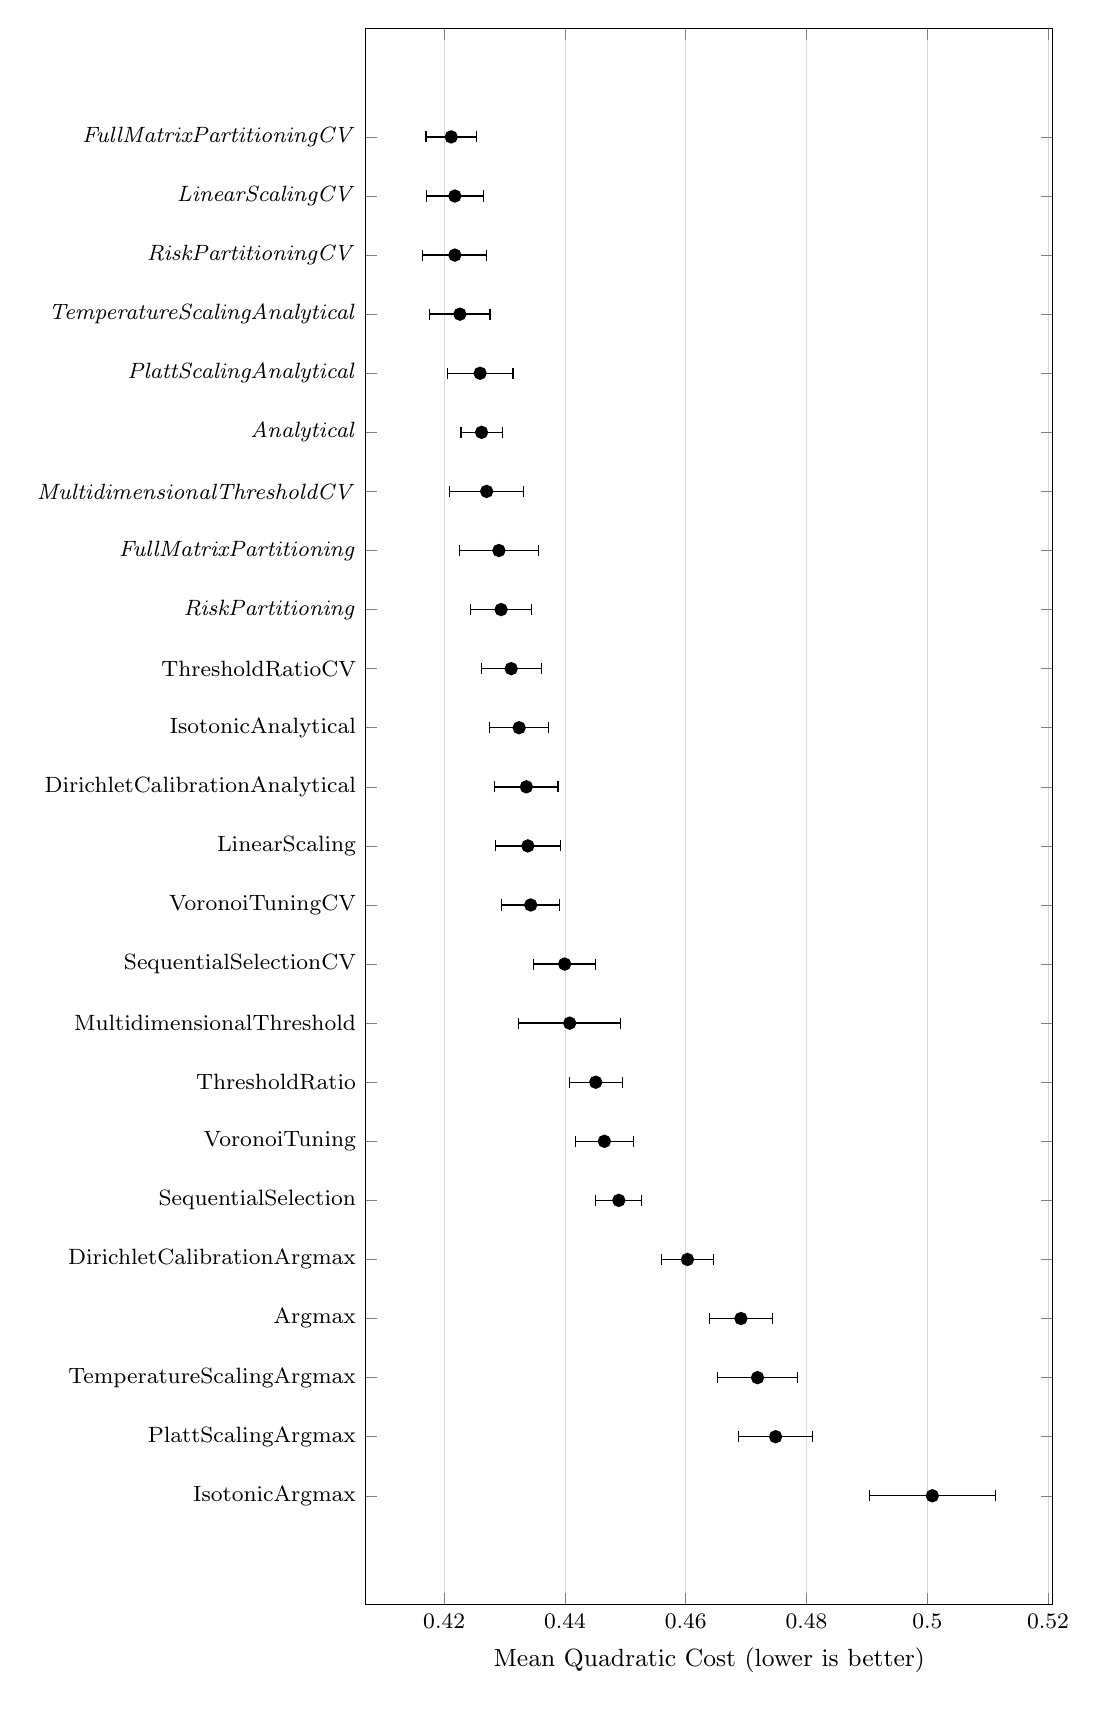
\begin{tikzpicture}
\begin{axis}[
    width=0.85\textwidth, height=21.60cm,
    xlabel={Mean Quadratic Cost (lower is better)},
    symbolic y coords={{FullMatrixPartitioningCV},{LinearScalingCV},{RiskPartitioningCV},{TemperatureScalingAnalytical},{PlattScalingAnalytical},{Analytical},{MultidimensionalThresholdCV},{FullMatrixPartitioning},{RiskPartitioning},{ThresholdRatioCV},{IsotonicAnalytical},{DirichletCalibrationAnalytical},{LinearScaling},{VoronoiTuningCV},{SequentialSelectionCV},{MultidimensionalThreshold},{ThresholdRatio},{VoronoiTuning},{SequentialSelection},{DirichletCalibrationArgmax},{Argmax},{TemperatureScalingArgmax},{PlattScalingArgmax},{IsotonicArgmax}},
    ytick={{FullMatrixPartitioningCV},{LinearScalingCV},{RiskPartitioningCV},{TemperatureScalingAnalytical},{PlattScalingAnalytical},{Analytical},{MultidimensionalThresholdCV},{FullMatrixPartitioning},{RiskPartitioning},{ThresholdRatioCV},{IsotonicAnalytical},{DirichletCalibrationAnalytical},{LinearScaling},{VoronoiTuningCV},{SequentialSelectionCV},{MultidimensionalThreshold},{ThresholdRatio},{VoronoiTuning},{SequentialSelection},{DirichletCalibrationArgmax},{Argmax},{TemperatureScalingArgmax},{PlattScalingArgmax},{IsotonicArgmax}},
    yticklabels={\textit{FullMatrixPartitioningCV},\textit{LinearScalingCV},\textit{RiskPartitioningCV},\textit{TemperatureScalingAnalytical},\textit{PlattScalingAnalytical},\textit{Analytical},\textit{MultidimensionalThresholdCV},\textit{FullMatrixPartitioning},\textit{RiskPartitioning},ThresholdRatioCV,IsotonicAnalytical,DirichletCalibrationAnalytical,LinearScaling,VoronoiTuningCV,SequentialSelectionCV,MultidimensionalThreshold,ThresholdRatio,VoronoiTuning,SequentialSelection,DirichletCalibrationArgmax,Argmax,TemperatureScalingArgmax,PlattScalingArgmax,IsotonicArgmax},
    y dir=reverse,
    enlarge y limits=0.08,
    xmajorgrids=true,
    major grid style={draw=black!15, line width=0.3pt},
    scaled x ticks=false,
    xticklabel style={/pgf/number format/fixed, /pgf/number format/precision=3},
    tick label style={font=\footnotesize},
    label style={font=\small},
    every axis plot/.append style={thick},
]
\addplot[only marks, mark=*, mark size=2pt, color=black, error bars/x dir=both, error bars/x explicit, error bars/error bar style={color=black, line width=0.5pt}] coordinates { (0.421172,{FullMatrixPartitioningCV}) +- (0.00416834,0) };
\addplot[only marks, mark=*, mark size=2pt, color=black, error bars/x dir=both, error bars/x explicit, error bars/error bar style={color=black, line width=0.5pt}] coordinates { (0.42177,{LinearScalingCV}) +- (0.00469818,0) };
\addplot[only marks, mark=*, mark size=2pt, color=black, error bars/x dir=both, error bars/x explicit, error bars/error bar style={color=black, line width=0.5pt}] coordinates { (0.42177,{RiskPartitioningCV}) +- (0.00528125,0) };
\addplot[only marks, mark=*, mark size=2pt, color=black, error bars/x dir=both, error bars/x explicit, error bars/error bar style={color=black, line width=0.5pt}] coordinates { (0.422608,{TemperatureScalingAnalytical}) +- (0.0049866,0) };
\addplot[only marks, mark=*, mark size=2pt, color=black, error bars/x dir=both, error bars/x explicit, error bars/error bar style={color=black, line width=0.5pt}] coordinates { (0.425957,{PlattScalingAnalytical}) +- (0.00544211,0) };
\addplot[only marks, mark=*, mark size=2pt, color=black, error bars/x dir=both, error bars/x explicit, error bars/error bar style={color=black, line width=0.5pt}] coordinates { (0.426196,{Analytical}) +- (0.00340226,0) };
\addplot[only marks, mark=*, mark size=2pt, color=black, error bars/x dir=both, error bars/x explicit, error bars/error bar style={color=black, line width=0.5pt}] coordinates { (0.427033,{MultidimensionalThresholdCV}) +- (0.00608365,0) };
\addplot[only marks, mark=*, mark size=2pt, color=black, error bars/x dir=both, error bars/x explicit, error bars/error bar style={color=black, line width=0.5pt}] coordinates { (0.429067,{FullMatrixPartitioning}) +- (0.00654211,0) };
\addplot[only marks, mark=*, mark size=2pt, color=black, error bars/x dir=both, error bars/x explicit, error bars/error bar style={color=black, line width=0.5pt}] coordinates { (0.429426,{RiskPartitioning}) +- (0.00501822,0) };
\addplot[only marks, mark=*, mark size=2pt, color=black, error bars/x dir=both, error bars/x explicit, error bars/error bar style={color=black, line width=0.5pt}] coordinates { (0.4311,{ThresholdRatioCV}) +- (0.0049551,0) };
\addplot[only marks, mark=*, mark size=2pt, color=black, error bars/x dir=both, error bars/x explicit, error bars/error bar style={color=black, line width=0.5pt}] coordinates { (0.432416,{IsotonicAnalytical}) +- (0.00489392,0) };
\addplot[only marks, mark=*, mark size=2pt, color=black, error bars/x dir=both, error bars/x explicit, error bars/error bar style={color=black, line width=0.5pt}] coordinates { (0.433612,{DirichletCalibrationAnalytical}) +- (0.00524818,0) };
\addplot[only marks, mark=*, mark size=2pt, color=black, error bars/x dir=both, error bars/x explicit, error bars/error bar style={color=black, line width=0.5pt}] coordinates { (0.433852,{LinearScaling}) +- (0.00535553,0) };
\addplot[only marks, mark=*, mark size=2pt, color=black, error bars/x dir=both, error bars/x explicit, error bars/error bar style={color=black, line width=0.5pt}] coordinates { (0.43433,{VoronoiTuningCV}) +- (0.00476955,0) };
\addplot[only marks, mark=*, mark size=2pt, color=black, error bars/x dir=both, error bars/x explicit, error bars/error bar style={color=black, line width=0.5pt}] coordinates { (0.439952,{SequentialSelectionCV}) +- (0.00509619,0) };
\addplot[only marks, mark=*, mark size=2pt, color=black, error bars/x dir=both, error bars/x explicit, error bars/error bar style={color=black, line width=0.5pt}] coordinates { (0.440789,{MultidimensionalThreshold}) +- (0.00843233,0) };
\addplot[only marks, mark=*, mark size=2pt, color=black, error bars/x dir=both, error bars/x explicit, error bars/error bar style={color=black, line width=0.5pt}] coordinates { (0.445096,{ThresholdRatio}) +- (0.00438397,0) };
\addplot[only marks, mark=*, mark size=2pt, color=black, error bars/x dir=both, error bars/x explicit, error bars/error bar style={color=black, line width=0.5pt}] coordinates { (0.446531,{VoronoiTuning}) +- (0.00475151,0) };
\addplot[only marks, mark=*, mark size=2pt, color=black, error bars/x dir=both, error bars/x explicit, error bars/error bar style={color=black, line width=0.5pt}] coordinates { (0.448923,{SequentialSelection}) +- (0.00380797,0) };
\addplot[only marks, mark=*, mark size=2pt, color=black, error bars/x dir=both, error bars/x explicit, error bars/error bar style={color=black, line width=0.5pt}] coordinates { (0.460287,{DirichletCalibrationArgmax}) +- (0.00435614,0) };
\addplot[only marks, mark=*, mark size=2pt, color=black, error bars/x dir=both, error bars/x explicit, error bars/error bar style={color=black, line width=0.5pt}] coordinates { (0.469139,{Argmax}) +- (0.00524985,0) };
\addplot[only marks, mark=*, mark size=2pt, color=black, error bars/x dir=both, error bars/x explicit, error bars/error bar style={color=black, line width=0.5pt}] coordinates { (0.47189,{TemperatureScalingArgmax}) +- (0.0066175,0) };
\addplot[only marks, mark=*, mark size=2pt, color=black, error bars/x dir=both, error bars/x explicit, error bars/error bar style={color=black, line width=0.5pt}] coordinates { (0.47488,{PlattScalingArgmax}) +- (0.00615896,0) };
\addplot[only marks, mark=*, mark size=2pt, color=black, error bars/x dir=both, error bars/x explicit, error bars/error bar style={color=black, line width=0.5pt}] coordinates { (0.500837,{IsotonicArgmax}) +- (0.0104509,0) };
\end{axis}
\end{tikzpicture}%
}
\caption{abalone: Quadratic Cost on LGBM (lower is better). Each dot is a strategy's mean over ten seeds with a $\pm 1$ SE horizontal bar; rows are sorted by mean, and the best strategy and any whose interval overlaps it are italicized.}%
\label{fig:ci-abalone-quadratic_cost}
\end{figure}


\subsection{Calibration in the multiclass simplex}

The parametric calibrate-then-analytical pipelines have win-or-tie rates between $30\%$ (Dirichlet) and $53\%$ (Temperature) on cost cells, against $79$ to $80\%$ for the three leading CV variants. DirichletCalibrationArgmax sits near the floor at $8\%$ on cost.

The calibrators are fit on the dedicated $10\%$ validation partition, while the cross-validated tuning variants use the full $80\%$ pool (roughly seven times the label budget). Whether matched-budget calibration would close the gap is outside the scope of this work, since the natural budget-matching protocols change what ``calibration'' denotes in the comparison (Chapter~\ref{sec:conclusion} discusses this).

\subsection{Vector-tuned versus Voronoi partitioning}

The Voronoi class contains the parallel-shift class and can rotate boundaries (Section~\ref{sec:voronoi_tessellation}, Proposition~\ref{prop:ps_in_vor}). Under the SE-overlap rule, partition by per-cell winning family:
\begin{itemize}
    \item Cost cells: a vector-tuned variant alone is in the winning band on $52\%$ of cells, both families share the band on $38\%$, a Voronoi variant alone on $0.1\%$, and neither on $9\%$.
    \item Maximization cells: both families share the band on $76\%$, vector-tuned alone on $18\%$, Voronoi alone on $1.2\%$, neither on $5\%$.
\end{itemize}
Voronoi variants are therefore rarely the unique winning family. On cost cells they are typically below the SE band; on maximization cells they typically share it with the vector-tuned methods.

This is consistent with Proposition~\ref{prop:ps_in_vor}: containment is population-level. The strict separation of Theorem~\ref{thm:rotational_dominance} requires a rotational regime the OpenML pool does not appear to concentrate in. The extra Voronoi parameters do not earn back their validation cost under the shared $10\%$ split.

\subsection{Cross-validated tuning variants}

Each cross-validated tuning variant has a higher cost win-or-tie rate than its single-split counterpart. Among the leading CV variants, the gap to the corresponding single-split variant is large: RiskPartitioningCV $79\%$ versus RiskPartitioning $29\%$, LinearScalingCV $78\%$ versus LinearScaling $30\%$, FullMatrixPartitioningCV $80\%$ versus FullMatrixPartitioning $34\%$. The single-split variants tune on the same $10\%$ validation partition the calibrators use; the CV variants tune over the full $80\%$ pool.

The cross-validated variant is therefore the recommended default for cost-sensitive multiclass decisions on benchmark pools of this scale.

\subsection{Non-decomposable maximization objectives}

For the macro $F_\beta$ metrics, MCC, and macro G-Mean the cross-validated tuning variants lead. The top is ThresholdRatioCV at $90\%$, with SequentialSelectionCV ($83\%$) and VoronoiTuningCV ($76\%$) next; Argmax sits at $62\%$. The calibrate-then-Argmax strategies fall in the $13$ to $41\%$ range.

Figure~\ref{fig:ci-fot_proving-f2_macro} shows a representative cell, \textit{fot\_proving} with LGBM on macro $F_2$: the cross-validated tuning variants cluster at the top within a narrow band, with Argmax among them, and the calibrate-then-Argmax strategies a few points below.

% Auto-generated by experiments.analysis.generate_ci_plots --- do not edit.
\begin{figure}[H]
\centering
\adjustbox{max width=\textwidth}{%
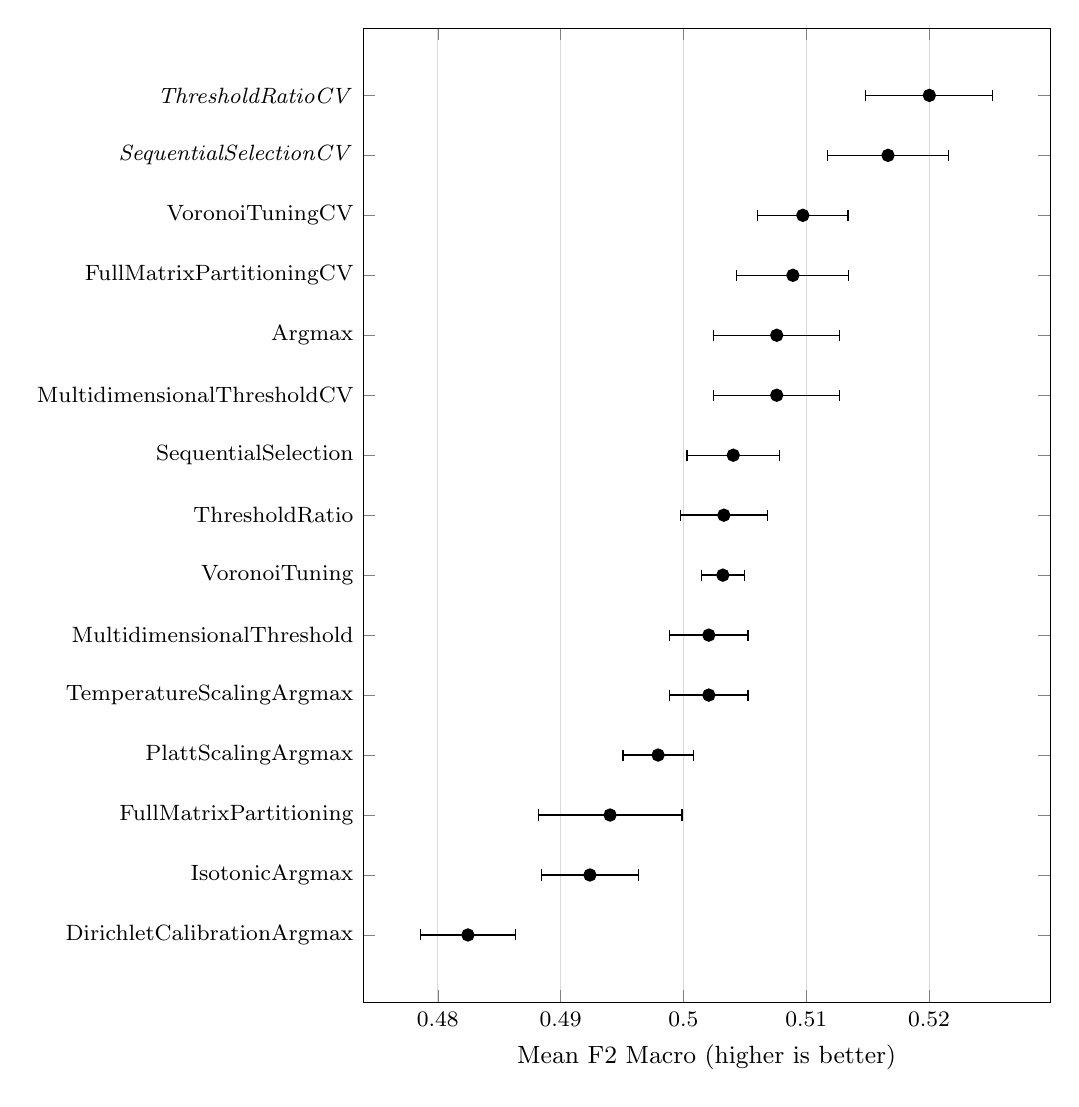
\begin{tikzpicture}
\begin{axis}[
    width=0.85\textwidth, height=13.95cm,
    xlabel={Mean F2 Macro (higher is better)},
    symbolic y coords={{ThresholdRatioCV},{SequentialSelectionCV},{VoronoiTuningCV},{FullMatrixPartitioningCV},{Argmax},{MultidimensionalThresholdCV},{SequentialSelection},{ThresholdRatio},{VoronoiTuning},{MultidimensionalThreshold},{TemperatureScalingArgmax},{PlattScalingArgmax},{FullMatrixPartitioning},{IsotonicArgmax},{DirichletCalibrationArgmax}},
    ytick={{ThresholdRatioCV},{SequentialSelectionCV},{VoronoiTuningCV},{FullMatrixPartitioningCV},{Argmax},{MultidimensionalThresholdCV},{SequentialSelection},{ThresholdRatio},{VoronoiTuning},{MultidimensionalThreshold},{TemperatureScalingArgmax},{PlattScalingArgmax},{FullMatrixPartitioning},{IsotonicArgmax},{DirichletCalibrationArgmax}},
    yticklabels={\textit{ThresholdRatioCV},\textit{SequentialSelectionCV},VoronoiTuningCV,FullMatrixPartitioningCV,Argmax,MultidimensionalThresholdCV,SequentialSelection,ThresholdRatio,VoronoiTuning,MultidimensionalThreshold,TemperatureScalingArgmax,PlattScalingArgmax,FullMatrixPartitioning,IsotonicArgmax,DirichletCalibrationArgmax},
    y dir=reverse,
    enlarge y limits=0.08,
    xmajorgrids=true,
    major grid style={draw=black!15, line width=0.3pt},
    scaled x ticks=false,
    xticklabel style={/pgf/number format/fixed, /pgf/number format/precision=3},
    tick label style={font=\footnotesize},
    label style={font=\small},
    every axis plot/.append style={thick},
]
\addplot[only marks, mark=*, mark size=2pt, color=black, error bars/x dir=both, error bars/x explicit, error bars/error bar style={color=black, line width=0.5pt}] coordinates { (0.520024,{ThresholdRatioCV}) +- (0.00517868,0) };
\addplot[only marks, mark=*, mark size=2pt, color=black, error bars/x dir=both, error bars/x explicit, error bars/error bar style={color=black, line width=0.5pt}] coordinates { (0.51666,{SequentialSelectionCV}) +- (0.00495574,0) };
\addplot[only marks, mark=*, mark size=2pt, color=black, error bars/x dir=both, error bars/x explicit, error bars/error bar style={color=black, line width=0.5pt}] coordinates { (0.509723,{VoronoiTuningCV}) +- (0.0036767,0) };
\addplot[only marks, mark=*, mark size=2pt, color=black, error bars/x dir=both, error bars/x explicit, error bars/error bar style={color=black, line width=0.5pt}] coordinates { (0.508913,{FullMatrixPartitioningCV}) +- (0.00455732,0) };
\addplot[only marks, mark=*, mark size=2pt, color=black, error bars/x dir=both, error bars/x explicit, error bars/error bar style={color=black, line width=0.5pt}] coordinates { (0.507598,{Argmax}) +- (0.00512521,0) };
\addplot[only marks, mark=*, mark size=2pt, color=black, error bars/x dir=both, error bars/x explicit, error bars/error bar style={color=black, line width=0.5pt}] coordinates { (0.507598,{MultidimensionalThresholdCV}) +- (0.00512521,0) };
\addplot[only marks, mark=*, mark size=2pt, color=black, error bars/x dir=both, error bars/x explicit, error bars/error bar style={color=black, line width=0.5pt}] coordinates { (0.504059,{SequentialSelection}) +- (0.00376794,0) };
\addplot[only marks, mark=*, mark size=2pt, color=black, error bars/x dir=both, error bars/x explicit, error bars/error bar style={color=black, line width=0.5pt}] coordinates { (0.503293,{ThresholdRatio}) +- (0.00352692,0) };
\addplot[only marks, mark=*, mark size=2pt, color=black, error bars/x dir=both, error bars/x explicit, error bars/error bar style={color=black, line width=0.5pt}] coordinates { (0.503212,{VoronoiTuning}) +- (0.00173639,0) };
\addplot[only marks, mark=*, mark size=2pt, color=black, error bars/x dir=both, error bars/x explicit, error bars/error bar style={color=black, line width=0.5pt}] coordinates { (0.502071,{MultidimensionalThreshold}) +- (0.00318547,0) };
\addplot[only marks, mark=*, mark size=2pt, color=black, error bars/x dir=both, error bars/x explicit, error bars/error bar style={color=black, line width=0.5pt}] coordinates { (0.502071,{TemperatureScalingArgmax}) +- (0.00318547,0) };
\addplot[only marks, mark=*, mark size=2pt, color=black, error bars/x dir=both, error bars/x explicit, error bars/error bar style={color=black, line width=0.5pt}] coordinates { (0.49794,{PlattScalingArgmax}) +- (0.00286004,0) };
\addplot[only marks, mark=*, mark size=2pt, color=black, error bars/x dir=both, error bars/x explicit, error bars/error bar style={color=black, line width=0.5pt}] coordinates { (0.494029,{FullMatrixPartitioning}) +- (0.00585333,0) };
\addplot[only marks, mark=*, mark size=2pt, color=black, error bars/x dir=both, error bars/x explicit, error bars/error bar style={color=black, line width=0.5pt}] coordinates { (0.492389,{IsotonicArgmax}) +- (0.00395195,0) };
\addplot[only marks, mark=*, mark size=2pt, color=black, error bars/x dir=both, error bars/x explicit, error bars/error bar style={color=black, line width=0.5pt}] coordinates { (0.482454,{DirichletCalibrationArgmax}) +- (0.00386869,0) };
\end{axis}
\end{tikzpicture}%
}
\caption{fot\_proving: F2 Macro on LGBM (higher is better). Each dot is a strategy's mean over ten seeds with a $\pm 1$ SE horizontal bar; rows are sorted by mean, and the best strategy and any whose interval overlaps it are italicized.}%
\label{fig:ci-fot_proving-f2_macro}
\end{figure}


Figures~\ref{fig:win-counts-multiclass-cost} and~\ref{fig:win-counts-multiclass-max} give the per-strategy win and tie rates under the $\pm 1$ SE overlap rule, broken out by base classifier and by dataset size and imbalance bucket; the figure captions document the reading convention and the bootstrap half-width. The dominant pattern on both objective groups is the gap between each cross-validated tuning variant and its single-split counterpart. DirichletCalibrationArgmax sits near the floor on every slice.

% Auto-generated by experiments.analysis.generate_win_counts --- do not edit.
\begin{figure}[H]
\centering
\adjustbox{max width=\textwidth}{%
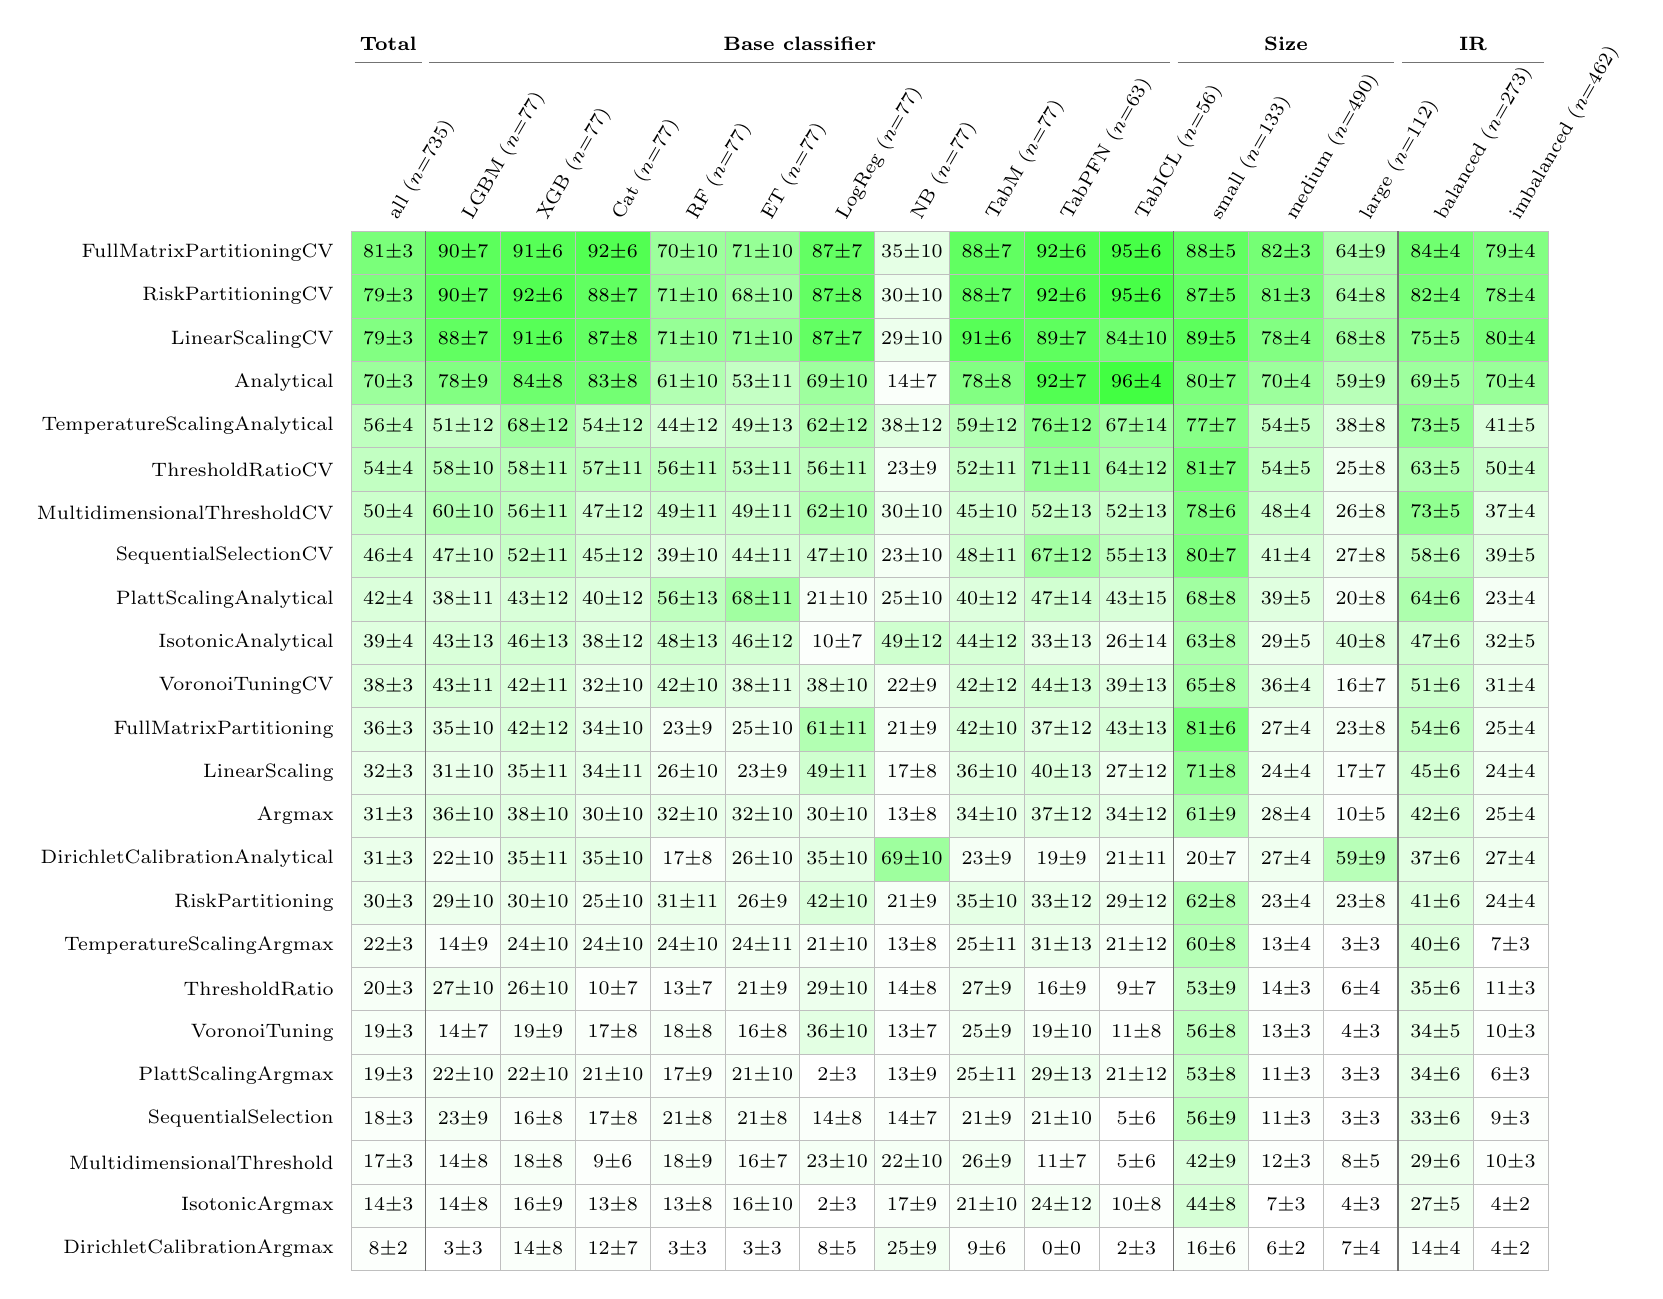
\begin{tikzpicture}[
    x=0.95cm, y=0.55cm,
    cell/.style={rectangle, draw=black!25, line width=0.2pt,
        minimum width=0.95cm, minimum height=0.55cm,
        anchor=center, font=\scriptsize, inner sep=0pt},
    rowlbl/.style={font=\scriptsize, anchor=east},
    collbl/.style={font=\scriptsize, anchor=west, rotate=60},
    grouplbl/.style={font=\scriptsize\bfseries, anchor=south},
    sep/.style={draw=black!55, line width=0.5pt},
]
\node[cell, fill=green!52] at (1, 24) {$81{\pm}3$};
\node[cell, fill=green!64] at (2, 24) {$90{\pm}7$};
\node[cell, fill=green!66] at (3, 24) {$91{\pm}6$};
\node[cell, fill=green!68] at (4, 24) {$92{\pm}6$};
\node[cell, fill=green!39] at (5, 24) {$70{\pm}10$};
\node[cell, fill=green!41] at (6, 24) {$71{\pm}10$};
\node[cell, fill=green!61] at (7, 24) {$87{\pm}7$};
\node[cell, fill=green!10] at (8, 24) {$35{\pm}10$};
\node[cell, fill=green!62] at (9, 24) {$88{\pm}7$};
\node[cell, fill=green!68] at (10, 24) {$92{\pm}6$};
\node[cell, fill=green!72] at (11, 24) {$95{\pm}6$};
\node[cell, fill=green!62] at (12, 24) {$88{\pm}5$};
\node[cell, fill=green!54] at (13, 24) {$82{\pm}3$};
\node[cell, fill=green!33] at (14, 24) {$64{\pm}9$};
\node[cell, fill=green!56] at (15, 24) {$84{\pm}4$};
\node[cell, fill=green!49] at (16, 24) {$79{\pm}4$};
\node[cell, fill=green!51] at (1, 23) {$79{\pm}3$};
\node[cell, fill=green!64] at (2, 23) {$90{\pm}7$};
\node[cell, fill=green!68] at (3, 23) {$92{\pm}6$};
\node[cell, fill=green!62] at (4, 23) {$88{\pm}7$};
\node[cell, fill=green!41] at (5, 23) {$71{\pm}10$};
\node[cell, fill=green!36] at (6, 23) {$68{\pm}10$};
\node[cell, fill=green!61] at (7, 23) {$87{\pm}8$};
\node[cell, fill=green!7] at (8, 23) {$30{\pm}10$};
\node[cell, fill=green!62] at (9, 23) {$88{\pm}7$};
\node[cell, fill=green!68] at (10, 23) {$92{\pm}6$};
\node[cell, fill=green!72] at (11, 23) {$95{\pm}6$};
\node[cell, fill=green!61] at (12, 23) {$87{\pm}5$};
\node[cell, fill=green!52] at (13, 23) {$81{\pm}3$};
\node[cell, fill=green!33] at (14, 23) {$64{\pm}8$};
\node[cell, fill=green!53] at (15, 23) {$82{\pm}4$};
\node[cell, fill=green!49] at (16, 23) {$78{\pm}4$};
\node[cell, fill=green!49] at (1, 22) {$79{\pm}3$};
\node[cell, fill=green!62] at (2, 22) {$88{\pm}7$};
\node[cell, fill=green!66] at (3, 22) {$91{\pm}6$};
\node[cell, fill=green!61] at (4, 22) {$87{\pm}8$};
\node[cell, fill=green!41] at (5, 22) {$71{\pm}10$};
\node[cell, fill=green!41] at (6, 22) {$71{\pm}10$};
\node[cell, fill=green!61] at (7, 22) {$87{\pm}7$};
\node[cell, fill=green!7] at (8, 22) {$29{\pm}10$};
\node[cell, fill=green!66] at (9, 22) {$91{\pm}6$};
\node[cell, fill=green!63] at (10, 22) {$89{\pm}7$};
\node[cell, fill=green!56] at (11, 22) {$84{\pm}10$};
\node[cell, fill=green!64] at (12, 22) {$89{\pm}5$};
\node[cell, fill=green!49] at (13, 22) {$78{\pm}4$};
\node[cell, fill=green!37] at (14, 22) {$68{\pm}8$};
\node[cell, fill=green!46] at (15, 22) {$75{\pm}5$};
\node[cell, fill=green!52] at (16, 22) {$80{\pm}4$};
\node[cell, fill=green!39] at (1, 21) {$70{\pm}3$};
\node[cell, fill=green!49] at (2, 21) {$78{\pm}9$};
\node[cell, fill=green!57] at (3, 21) {$84{\pm}8$};
\node[cell, fill=green!55] at (4, 21) {$83{\pm}8$};
\node[cell, fill=green!30] at (5, 21) {$61{\pm}10$};
\node[cell, fill=green!23] at (6, 21) {$53{\pm}11$};
\node[cell, fill=green!38] at (7, 21) {$69{\pm}10$};
\node[cell, fill=green!2] at (8, 21) {$14{\pm}7$};
\node[cell, fill=green!49] at (9, 21) {$78{\pm}8$};
\node[cell, fill=green!68] at (10, 21) {$92{\pm}7$};
\node[cell, fill=green!74] at (11, 21) {$96{\pm}4$};
\node[cell, fill=green!51] at (12, 21) {$80{\pm}7$};
\node[cell, fill=green!39] at (13, 21) {$70{\pm}4$};
\node[cell, fill=green!28] at (14, 21) {$59{\pm}9$};
\node[cell, fill=green!38] at (15, 21) {$69{\pm}5$};
\node[cell, fill=green!40] at (16, 21) {$70{\pm}4$};
\node[cell, fill=green!25] at (1, 20) {$56{\pm}4$};
\node[cell, fill=green!21] at (2, 20) {$51{\pm}12$};
\node[cell, fill=green!37] at (3, 20) {$68{\pm}12$};
\node[cell, fill=green!23] at (4, 20) {$54{\pm}12$};
\node[cell, fill=green!16] at (5, 20) {$44{\pm}12$};
\node[cell, fill=green!19] at (6, 20) {$49{\pm}13$};
\node[cell, fill=green!31] at (7, 20) {$62{\pm}12$};
\node[cell, fill=green!12] at (8, 20) {$38{\pm}12$};
\node[cell, fill=green!28] at (9, 20) {$59{\pm}12$};
\node[cell, fill=green!46] at (10, 20) {$76{\pm}12$};
\node[cell, fill=green!36] at (11, 20) {$67{\pm}14$};
\node[cell, fill=green!47] at (12, 20) {$77{\pm}7$};
\node[cell, fill=green!23] at (13, 20) {$54{\pm}5$};
\node[cell, fill=green!11] at (14, 20) {$38{\pm}8$};
\node[cell, fill=green!43] at (15, 20) {$73{\pm}5$};
\node[cell, fill=green!14] at (16, 20) {$41{\pm}5$};
\node[cell, fill=green!24] at (1, 19) {$54{\pm}4$};
\node[cell, fill=green!27] at (2, 19) {$58{\pm}10$};
\node[cell, fill=green!27] at (3, 19) {$58{\pm}11$};
\node[cell, fill=green!26] at (4, 19) {$57{\pm}11$};
\node[cell, fill=green!25] at (5, 19) {$56{\pm}11$};
\node[cell, fill=green!23] at (6, 19) {$53{\pm}11$};
\node[cell, fill=green!25] at (7, 19) {$56{\pm}11$};
\node[cell, fill=green!4] at (8, 19) {$23{\pm}9$};
\node[cell, fill=green!22] at (9, 19) {$52{\pm}11$};
\node[cell, fill=green!41] at (10, 19) {$71{\pm}11$};
\node[cell, fill=green!33] at (11, 19) {$64{\pm}12$};
\node[cell, fill=green!53] at (12, 19) {$81{\pm}7$};
\node[cell, fill=green!23] at (13, 19) {$54{\pm}5$};
\node[cell, fill=green!5] at (14, 19) {$25{\pm}8$};
\node[cell, fill=green!31] at (15, 19) {$63{\pm}5$};
\node[cell, fill=green!20] at (16, 19) {$50{\pm}4$};
\node[cell, fill=green!20] at (1, 18) {$50{\pm}4$};
\node[cell, fill=green!29] at (2, 18) {$60{\pm}10$};
\node[cell, fill=green!25] at (3, 18) {$56{\pm}11$};
\node[cell, fill=green!17] at (4, 18) {$47{\pm}12$};
\node[cell, fill=green!19] at (5, 18) {$49{\pm}11$};
\node[cell, fill=green!19] at (6, 18) {$49{\pm}11$};
\node[cell, fill=green!31] at (7, 18) {$62{\pm}10$};
\node[cell, fill=green!7] at (8, 18) {$30{\pm}10$};
\node[cell, fill=green!17] at (9, 18) {$45{\pm}10$};
\node[cell, fill=green!22] at (10, 18) {$52{\pm}13$};
\node[cell, fill=green!21] at (11, 18) {$52{\pm}13$};
\node[cell, fill=green!49] at (12, 18) {$78{\pm}6$};
\node[cell, fill=green!19] at (13, 18) {$48{\pm}4$};
\node[cell, fill=green!5] at (14, 18) {$26{\pm}8$};
\node[cell, fill=green!43] at (15, 18) {$73{\pm}5$};
\node[cell, fill=green!11] at (16, 18) {$37{\pm}4$};
\node[cell, fill=green!17] at (1, 17) {$46{\pm}4$};
\node[cell, fill=green!17] at (2, 17) {$47{\pm}10$};
\node[cell, fill=green!22] at (3, 17) {$52{\pm}11$};
\node[cell, fill=green!17] at (4, 17) {$45{\pm}12$};
\node[cell, fill=green!12] at (5, 17) {$39{\pm}10$};
\node[cell, fill=green!16] at (6, 17) {$44{\pm}11$};
\node[cell, fill=green!17] at (7, 17) {$47{\pm}10$};
\node[cell, fill=green!4] at (8, 17) {$23{\pm}10$};
\node[cell, fill=green!18] at (9, 17) {$48{\pm}11$};
\node[cell, fill=green!36] at (10, 17) {$67{\pm}12$};
\node[cell, fill=green!25] at (11, 17) {$55{\pm}13$};
\node[cell, fill=green!51] at (12, 17) {$80{\pm}7$};
\node[cell, fill=green!14] at (13, 17) {$41{\pm}4$};
\node[cell, fill=green!6] at (14, 17) {$27{\pm}8$};
\node[cell, fill=green!26] at (15, 17) {$58{\pm}6$};
\node[cell, fill=green!12] at (16, 17) {$39{\pm}5$};
\node[cell, fill=green!14] at (1, 16) {$42{\pm}4$};
\node[cell, fill=green!12] at (2, 16) {$38{\pm}11$};
\node[cell, fill=green!15] at (3, 16) {$43{\pm}12$};
\node[cell, fill=green!13] at (4, 16) {$40{\pm}12$};
\node[cell, fill=green!25] at (5, 16) {$56{\pm}13$};
\node[cell, fill=green!37] at (6, 16) {$68{\pm}11$};
\node[cell, fill=green!3] at (7, 16) {$21{\pm}10$};
\node[cell, fill=green!5] at (8, 16) {$25{\pm}10$};
\node[cell, fill=green!13] at (9, 16) {$40{\pm}12$};
\node[cell, fill=green!18] at (10, 16) {$47{\pm}14$};
\node[cell, fill=green!15] at (11, 16) {$43{\pm}15$};
\node[cell, fill=green!37] at (12, 16) {$68{\pm}8$};
\node[cell, fill=green!12] at (13, 16) {$39{\pm}5$};
\node[cell, fill=green!3] at (14, 16) {$20{\pm}8$};
\node[cell, fill=green!32] at (15, 16) {$64{\pm}6$};
\node[cell, fill=green!4] at (16, 16) {$23{\pm}4$};
\node[cell, fill=green!12] at (1, 15) {$39{\pm}4$};
\node[cell, fill=green!15] at (2, 15) {$43{\pm}13$};
\node[cell, fill=green!17] at (3, 15) {$46{\pm}13$};
\node[cell, fill=green!12] at (4, 15) {$38{\pm}12$};
\node[cell, fill=green!18] at (5, 15) {$48{\pm}13$};
\node[cell, fill=green!17] at (6, 15) {$46{\pm}12$};
\node[cell, fill=green!1] at (7, 15) {$10{\pm}7$};
\node[cell, fill=green!19] at (8, 15) {$49{\pm}12$};
\node[cell, fill=green!16] at (9, 15) {$44{\pm}12$};
\node[cell, fill=green!9] at (10, 15) {$33{\pm}13$};
\node[cell, fill=green!5] at (11, 15) {$26{\pm}14$};
\node[cell, fill=green!32] at (12, 15) {$63{\pm}8$};
\node[cell, fill=green!7] at (13, 15) {$29{\pm}5$};
\node[cell, fill=green!13] at (14, 15) {$40{\pm}8$};
\node[cell, fill=green!18] at (15, 15) {$47{\pm}6$};
\node[cell, fill=green!8] at (16, 15) {$32{\pm}5$};
\node[cell, fill=green!12] at (1, 14) {$38{\pm}3$};
\node[cell, fill=green!15] at (2, 14) {$43{\pm}11$};
\node[cell, fill=green!14] at (3, 14) {$42{\pm}11$};
\node[cell, fill=green!8] at (4, 14) {$32{\pm}10$};
\node[cell, fill=green!14] at (5, 14) {$42{\pm}10$};
\node[cell, fill=green!11] at (6, 14) {$38{\pm}11$};
\node[cell, fill=green!11] at (7, 14) {$38{\pm}10$};
\node[cell, fill=green!4] at (8, 14) {$22{\pm}9$};
\node[cell, fill=green!14] at (9, 14) {$42{\pm}12$};
\node[cell, fill=green!16] at (10, 14) {$44{\pm}13$};
\node[cell, fill=green!12] at (11, 14) {$39{\pm}13$};
\node[cell, fill=green!34] at (12, 14) {$65{\pm}8$};
\node[cell, fill=green!10] at (13, 14) {$36{\pm}4$};
\node[cell, fill=green!2] at (14, 14) {$16{\pm}7$};
\node[cell, fill=green!20] at (15, 14) {$51{\pm}6$};
\node[cell, fill=green!7] at (16, 14) {$31{\pm}4$};
\node[cell, fill=green!10] at (1, 13) {$36{\pm}3$};
\node[cell, fill=green!10] at (2, 13) {$35{\pm}10$};
\node[cell, fill=green!14] at (3, 13) {$42{\pm}12$};
\node[cell, fill=green!9] at (4, 13) {$34{\pm}10$};
\node[cell, fill=green!4] at (5, 13) {$23{\pm}9$};
\node[cell, fill=green!5] at (6, 13) {$25{\pm}10$};
\node[cell, fill=green!30] at (7, 13) {$61{\pm}11$};
\node[cell, fill=green!3] at (8, 13) {$21{\pm}9$};
\node[cell, fill=green!14] at (9, 13) {$42{\pm}10$};
\node[cell, fill=green!11] at (10, 13) {$37{\pm}12$};
\node[cell, fill=green!15] at (11, 13) {$43{\pm}13$};
\node[cell, fill=green!53] at (12, 13) {$81{\pm}6$};
\node[cell, fill=green!6] at (13, 13) {$27{\pm}4$};
\node[cell, fill=green!4] at (14, 13) {$23{\pm}8$};
\node[cell, fill=green!23] at (15, 13) {$54{\pm}6$};
\node[cell, fill=green!5] at (16, 13) {$25{\pm}4$};
\node[cell, fill=green!8] at (1, 12) {$32{\pm}3$};
\node[cell, fill=green!8] at (2, 12) {$31{\pm}10$};
\node[cell, fill=green!10] at (3, 12) {$35{\pm}11$};
\node[cell, fill=green!9] at (4, 12) {$34{\pm}11$};
\node[cell, fill=green!5] at (5, 12) {$26{\pm}10$};
\node[cell, fill=green!4] at (6, 12) {$23{\pm}9$};
\node[cell, fill=green!19] at (7, 12) {$49{\pm}11$};
\node[cell, fill=green!2] at (8, 12) {$17{\pm}8$};
\node[cell, fill=green!11] at (9, 12) {$36{\pm}10$};
\node[cell, fill=green!13] at (10, 12) {$40{\pm}13$};
\node[cell, fill=green!6] at (11, 12) {$27{\pm}12$};
\node[cell, fill=green!41] at (12, 12) {$71{\pm}8$};
\node[cell, fill=green!5] at (13, 12) {$24{\pm}4$};
\node[cell, fill=green!2] at (14, 12) {$17{\pm}7$};
\node[cell, fill=green!17] at (15, 12) {$45{\pm}6$};
\node[cell, fill=green!5] at (16, 12) {$24{\pm}4$};
\node[cell, fill=green!8] at (1, 11) {$31{\pm}3$};
\node[cell, fill=green!11] at (2, 11) {$36{\pm}10$};
\node[cell, fill=green!11] at (3, 11) {$38{\pm}10$};
\node[cell, fill=green!7] at (4, 11) {$30{\pm}10$};
\node[cell, fill=green!8] at (5, 11) {$32{\pm}10$};
\node[cell, fill=green!8] at (6, 11) {$32{\pm}10$};
\node[cell, fill=green!7] at (7, 11) {$30{\pm}10$};
\node[cell, fill=green!1] at (8, 11) {$13{\pm}8$};
\node[cell, fill=green!9] at (9, 11) {$34{\pm}10$};
\node[cell, fill=green!11] at (10, 11) {$37{\pm}12$};
\node[cell, fill=green!9] at (11, 11) {$34{\pm}12$};
\node[cell, fill=green!30] at (12, 11) {$61{\pm}9$};
\node[cell, fill=green!6] at (13, 11) {$28{\pm}4$};
\node[cell, fill=green!1] at (14, 11) {$10{\pm}5$};
\node[cell, fill=green!14] at (15, 11) {$42{\pm}6$};
\node[cell, fill=green!5] at (16, 11) {$25{\pm}4$};
\node[cell, fill=green!8] at (1, 10) {$31{\pm}3$};
\node[cell, fill=green!4] at (2, 10) {$22{\pm}10$};
\node[cell, fill=green!10] at (3, 10) {$35{\pm}11$};
\node[cell, fill=green!10] at (4, 10) {$35{\pm}10$};
\node[cell, fill=green!2] at (5, 10) {$17{\pm}8$};
\node[cell, fill=green!5] at (6, 10) {$26{\pm}10$};
\node[cell, fill=green!10] at (7, 10) {$35{\pm}10$};
\node[cell, fill=green!38] at (8, 10) {$69{\pm}10$};
\node[cell, fill=green!4] at (9, 10) {$23{\pm}9$};
\node[cell, fill=green!3] at (10, 10) {$19{\pm}9$};
\node[cell, fill=green!4] at (11, 10) {$21{\pm}11$};
\node[cell, fill=green!3] at (12, 10) {$20{\pm}7$};
\node[cell, fill=green!6] at (13, 10) {$27{\pm}4$};
\node[cell, fill=green!28] at (14, 10) {$59{\pm}9$};
\node[cell, fill=green!11] at (15, 10) {$37{\pm}6$};
\node[cell, fill=green!6] at (16, 10) {$27{\pm}4$};
\node[cell, fill=green!7] at (1, 9) {$30{\pm}3$};
\node[cell, fill=green!7] at (2, 9) {$29{\pm}10$};
\node[cell, fill=green!7] at (3, 9) {$30{\pm}10$};
\node[cell, fill=green!5] at (4, 9) {$25{\pm}10$};
\node[cell, fill=green!8] at (5, 9) {$31{\pm}11$};
\node[cell, fill=green!5] at (6, 9) {$26{\pm}9$};
\node[cell, fill=green!14] at (7, 9) {$42{\pm}10$};
\node[cell, fill=green!3] at (8, 9) {$21{\pm}9$};
\node[cell, fill=green!10] at (9, 9) {$35{\pm}10$};
\node[cell, fill=green!9] at (10, 9) {$33{\pm}12$};
\node[cell, fill=green!7] at (11, 9) {$29{\pm}12$};
\node[cell, fill=green!30] at (12, 9) {$62{\pm}8$};
\node[cell, fill=green!4] at (13, 9) {$23{\pm}4$};
\node[cell, fill=green!4] at (14, 9) {$23{\pm}8$};
\node[cell, fill=green!13] at (15, 9) {$41{\pm}6$};
\node[cell, fill=green!4] at (16, 9) {$24{\pm}4$};
\node[cell, fill=green!4] at (1, 8) {$22{\pm}3$};
\node[cell, fill=green!2] at (2, 8) {$14{\pm}9$};
\node[cell, fill=green!5] at (3, 8) {$24{\pm}10$};
\node[cell, fill=green!5] at (4, 8) {$24{\pm}10$};
\node[cell, fill=green!5] at (5, 8) {$24{\pm}10$};
\node[cell, fill=green!5] at (6, 8) {$24{\pm}11$};
\node[cell, fill=green!3] at (7, 8) {$21{\pm}10$};
\node[cell, fill=green!1] at (8, 8) {$13{\pm}8$};
\node[cell, fill=green!5] at (9, 8) {$25{\pm}11$};
\node[cell, fill=green!7] at (10, 8) {$31{\pm}13$};
\node[cell, fill=green!4] at (11, 8) {$21{\pm}12$};
\node[cell, fill=green!29] at (12, 8) {$60{\pm}8$};
\node[cell, fill=green!1] at (13, 8) {$13{\pm}4$};
\node[cell, fill=green!0] at (14, 8) {$3{\pm}3$};
\node[cell, fill=green!13] at (15, 8) {$40{\pm}6$};
\node[cell, fill=green!0] at (16, 8) {$7{\pm}3$};
\node[cell, fill=green!3] at (1, 7) {$20{\pm}3$};
\node[cell, fill=green!6] at (2, 7) {$27{\pm}10$};
\node[cell, fill=green!5] at (3, 7) {$26{\pm}10$};
\node[cell, fill=green!1] at (4, 7) {$10{\pm}7$};
\node[cell, fill=green!1] at (5, 7) {$13{\pm}7$};
\node[cell, fill=green!3] at (6, 7) {$21{\pm}9$};
\node[cell, fill=green!7] at (7, 7) {$29{\pm}10$};
\node[cell, fill=green!2] at (8, 7) {$14{\pm}8$};
\node[cell, fill=green!6] at (9, 7) {$27{\pm}9$};
\node[cell, fill=green!2] at (10, 7) {$16{\pm}9$};
\node[cell, fill=green!1] at (11, 7) {$9{\pm}7$};
\node[cell, fill=green!22] at (12, 7) {$53{\pm}9$};
\node[cell, fill=green!1] at (13, 7) {$14{\pm}3$};
\node[cell, fill=green!0] at (14, 7) {$6{\pm}4$};
\node[cell, fill=green!10] at (15, 7) {$35{\pm}6$};
\node[cell, fill=green!1] at (16, 7) {$11{\pm}3$};
\node[cell, fill=green!3] at (1, 6) {$19{\pm}3$};
\node[cell, fill=green!2] at (2, 6) {$14{\pm}7$};
\node[cell, fill=green!3] at (3, 6) {$19{\pm}9$};
\node[cell, fill=green!2] at (4, 6) {$17{\pm}8$};
\node[cell, fill=green!3] at (5, 6) {$18{\pm}8$};
\node[cell, fill=green!2] at (6, 6) {$16{\pm}8$};
\node[cell, fill=green!11] at (7, 6) {$36{\pm}10$};
\node[cell, fill=green!1] at (8, 6) {$13{\pm}7$};
\node[cell, fill=green!5] at (9, 6) {$25{\pm}9$};
\node[cell, fill=green!3] at (10, 6) {$19{\pm}10$};
\node[cell, fill=green!1] at (11, 6) {$11{\pm}8$};
\node[cell, fill=green!25] at (12, 6) {$56{\pm}8$};
\node[cell, fill=green!1] at (13, 6) {$13{\pm}3$};
\node[cell, fill=green!0] at (14, 6) {$4{\pm}3$};
\node[cell, fill=green!9] at (15, 6) {$34{\pm}5$};
\node[cell, fill=green!1] at (16, 6) {$10{\pm}3$};
\node[cell, fill=green!3] at (1, 5) {$19{\pm}3$};
\node[cell, fill=green!4] at (2, 5) {$22{\pm}10$};
\node[cell, fill=green!4] at (3, 5) {$22{\pm}10$};
\node[cell, fill=green!3] at (4, 5) {$21{\pm}10$};
\node[cell, fill=green!2] at (5, 5) {$17{\pm}9$};
\node[cell, fill=green!3] at (6, 5) {$21{\pm}10$};
\node[cell, fill=green!0] at (7, 5) {$2{\pm}3$};
\node[cell, fill=green!1] at (8, 5) {$13{\pm}9$};
\node[cell, fill=green!5] at (9, 5) {$25{\pm}11$};
\node[cell, fill=green!7] at (10, 5) {$29{\pm}13$};
\node[cell, fill=green!4] at (11, 5) {$21{\pm}12$};
\node[cell, fill=green!22] at (12, 5) {$53{\pm}8$};
\node[cell, fill=green!1] at (13, 5) {$11{\pm}3$};
\node[cell, fill=green!0] at (14, 5) {$3{\pm}3$};
\node[cell, fill=green!9] at (15, 5) {$34{\pm}6$};
\node[cell, fill=green!0] at (16, 5) {$6{\pm}3$};
\node[cell, fill=green!2] at (1, 4) {$18{\pm}3$};
\node[cell, fill=green!4] at (2, 4) {$23{\pm}9$};
\node[cell, fill=green!2] at (3, 4) {$16{\pm}8$};
\node[cell, fill=green!2] at (4, 4) {$17{\pm}8$};
\node[cell, fill=green!3] at (5, 4) {$21{\pm}8$};
\node[cell, fill=green!3] at (6, 4) {$21{\pm}8$};
\node[cell, fill=green!2] at (7, 4) {$14{\pm}8$};
\node[cell, fill=green!2] at (8, 4) {$14{\pm}7$};
\node[cell, fill=green!3] at (9, 4) {$21{\pm}9$};
\node[cell, fill=green!3] at (10, 4) {$21{\pm}10$};
\node[cell, fill=green!0] at (11, 4) {$5{\pm}6$};
\node[cell, fill=green!25] at (12, 4) {$56{\pm}9$};
\node[cell, fill=green!1] at (13, 4) {$11{\pm}3$};
\node[cell, fill=green!0] at (14, 4) {$3{\pm}3$};
\node[cell, fill=green!9] at (15, 4) {$33{\pm}6$};
\node[cell, fill=green!1] at (16, 4) {$9{\pm}3$};
\node[cell, fill=green!2] at (1, 3) {$17{\pm}3$};
\node[cell, fill=green!2] at (2, 3) {$14{\pm}8$};
\node[cell, fill=green!3] at (3, 3) {$18{\pm}8$};
\node[cell, fill=green!1] at (4, 3) {$9{\pm}6$};
\node[cell, fill=green!3] at (5, 3) {$18{\pm}9$};
\node[cell, fill=green!2] at (6, 3) {$16{\pm}7$};
\node[cell, fill=green!4] at (7, 3) {$23{\pm}10$};
\node[cell, fill=green!4] at (8, 3) {$22{\pm}10$};
\node[cell, fill=green!5] at (9, 3) {$26{\pm}9$};
\node[cell, fill=green!1] at (10, 3) {$11{\pm}7$};
\node[cell, fill=green!0] at (11, 3) {$5{\pm}6$};
\node[cell, fill=green!14] at (12, 3) {$42{\pm}9$};
\node[cell, fill=green!1] at (13, 3) {$12{\pm}3$};
\node[cell, fill=green!1] at (14, 3) {$8{\pm}5$};
\node[cell, fill=green!7] at (15, 3) {$29{\pm}6$};
\node[cell, fill=green!1] at (16, 3) {$10{\pm}3$};
\node[cell, fill=green!2] at (1, 2) {$14{\pm}3$};
\node[cell, fill=green!2] at (2, 2) {$14{\pm}8$};
\node[cell, fill=green!2] at (3, 2) {$16{\pm}9$};
\node[cell, fill=green!1] at (4, 2) {$13{\pm}8$};
\node[cell, fill=green!1] at (5, 2) {$13{\pm}8$};
\node[cell, fill=green!2] at (6, 2) {$16{\pm}10$};
\node[cell, fill=green!0] at (7, 2) {$2{\pm}3$};
\node[cell, fill=green!2] at (8, 2) {$17{\pm}9$};
\node[cell, fill=green!3] at (9, 2) {$21{\pm}10$};
\node[cell, fill=green!5] at (10, 2) {$24{\pm}12$};
\node[cell, fill=green!1] at (11, 2) {$10{\pm}8$};
\node[cell, fill=green!16] at (12, 2) {$44{\pm}8$};
\node[cell, fill=green!0] at (13, 2) {$7{\pm}3$};
\node[cell, fill=green!0] at (14, 2) {$4{\pm}3$};
\node[cell, fill=green!6] at (15, 2) {$27{\pm}5$};
\node[cell, fill=green!0] at (16, 2) {$4{\pm}2$};
\node[cell, fill=green!1] at (1, 1) {$8{\pm}2$};
\node[cell, fill=green!0] at (2, 1) {$3{\pm}3$};
\node[cell, fill=green!2] at (3, 1) {$14{\pm}8$};
\node[cell, fill=green!1] at (4, 1) {$12{\pm}7$};
\node[cell, fill=green!0] at (5, 1) {$3{\pm}3$};
\node[cell, fill=green!0] at (6, 1) {$3{\pm}3$};
\node[cell, fill=green!0] at (7, 1) {$8{\pm}5$};
\node[cell, fill=green!5] at (8, 1) {$25{\pm}9$};
\node[cell, fill=green!1] at (9, 1) {$9{\pm}6$};
\node[cell, fill=green!0] at (10, 1) {$0{\pm}0$};
\node[cell, fill=green!0] at (11, 1) {$2{\pm}3$};
\node[cell, fill=green!2] at (12, 1) {$16{\pm}6$};
\node[cell, fill=green!0] at (13, 1) {$6{\pm}2$};
\node[cell, fill=green!0] at (14, 1) {$7{\pm}4$};
\node[cell, fill=green!2] at (15, 1) {$14{\pm}4$};
\node[cell, fill=green!0] at (16, 1) {$4{\pm}2$};
\node[rowlbl] at (0.4, 24) {FullMatrixPartitioningCV};
\node[rowlbl] at (0.4, 23) {RiskPartitioningCV};
\node[rowlbl] at (0.4, 22) {LinearScalingCV};
\node[rowlbl] at (0.4, 21) {Analytical};
\node[rowlbl] at (0.4, 20) {TemperatureScalingAnalytical};
\node[rowlbl] at (0.4, 19) {ThresholdRatioCV};
\node[rowlbl] at (0.4, 18) {MultidimensionalThresholdCV};
\node[rowlbl] at (0.4, 17) {SequentialSelectionCV};
\node[rowlbl] at (0.4, 16) {PlattScalingAnalytical};
\node[rowlbl] at (0.4, 15) {IsotonicAnalytical};
\node[rowlbl] at (0.4, 14) {VoronoiTuningCV};
\node[rowlbl] at (0.4, 13) {FullMatrixPartitioning};
\node[rowlbl] at (0.4, 12) {LinearScaling};
\node[rowlbl] at (0.4, 11) {Argmax};
\node[rowlbl] at (0.4, 10) {DirichletCalibrationAnalytical};
\node[rowlbl] at (0.4, 9) {RiskPartitioning};
\node[rowlbl] at (0.4, 8) {TemperatureScalingArgmax};
\node[rowlbl] at (0.4, 7) {ThresholdRatio};
\node[rowlbl] at (0.4, 6) {VoronoiTuning};
\node[rowlbl] at (0.4, 5) {PlattScalingArgmax};
\node[rowlbl] at (0.4, 4) {SequentialSelection};
\node[rowlbl] at (0.4, 3) {MultidimensionalThreshold};
\node[rowlbl] at (0.4, 2) {IsotonicArgmax};
\node[rowlbl] at (0.4, 1) {DirichletCalibrationArgmax};
\node[collbl] at (1, 24.6) {all ($n{=}735$)};
\node[collbl] at (2, 24.6) {LGBM ($n{=}77$)};
\node[collbl] at (3, 24.6) {XGB ($n{=}77$)};
\node[collbl] at (4, 24.6) {Cat ($n{=}77$)};
\node[collbl] at (5, 24.6) {RF ($n{=}77$)};
\node[collbl] at (6, 24.6) {ET ($n{=}77$)};
\node[collbl] at (7, 24.6) {LogReg ($n{=}77$)};
\node[collbl] at (8, 24.6) {NB ($n{=}77$)};
\node[collbl] at (9, 24.6) {TabM ($n{=}77$)};
\node[collbl] at (10, 24.6) {TabPFN ($n{=}63$)};
\node[collbl] at (11, 24.6) {TabICL ($n{=}56$)};
\node[collbl] at (12, 24.6) {small ($n{=}133$)};
\node[collbl] at (13, 24.6) {medium ($n{=}490$)};
\node[collbl] at (14, 24.6) {large ($n{=}112$)};
\node[collbl] at (15, 24.6) {balanced ($n{=}273$)};
\node[collbl] at (16, 24.6) {imbalanced ($n{=}462$)};
\draw[black!55, line width=0.5pt] (0.55, 28.4) -- (1.45, 28.4);
\node[grouplbl] at (1.0, 28.45) {Total};
\draw[black!55, line width=0.5pt] (1.55, 28.4) -- (11.45, 28.4);
\node[grouplbl] at (6.5, 28.45) {Base classifier};
\draw[black!55, line width=0.5pt] (11.55, 28.4) -- (14.45, 28.4);
\node[grouplbl] at (13.0, 28.45) {Size};
\draw[black!55, line width=0.5pt] (14.55, 28.4) -- (16.45, 28.4);
\node[grouplbl] at (15.5, 28.45) {IR};
\draw[sep] (1.5, 0.5) -- (1.5, 24.5);
\draw[sep] (11.5, 0.5) -- (11.5, 24.5);
\draw[sep] (14.5, 0.5) -- (14.5, 24.5);
\end{tikzpicture}%
}
\caption{Per-strategy win/tie rates on multiclass cost-matrix objectives. Each cell reads ``$r{\pm}H$'': $r$ is the percentage of (dataset, model, objective) cells in the slice where the strategy won or tied the per-row best under the $\pm 1$ SE overlap rule, and $H$ is the half-width of a 95\% cluster-bootstrap confidence interval for $r$ (percentage points). Shading is a quadratic ($\mathrm{rate}^2$) scale of $r$. Strategies are sorted by overall win rate; ``$n$'' under each column header is the maximum applicable cell count for that slice.}%
\label{fig:win-counts-multiclass-cost}
\end{figure}


% Auto-generated by experiments.analysis.generate_win_counts --- do not edit.
\begin{figure}[H]
\centering
\adjustbox{max width=\textwidth}{%
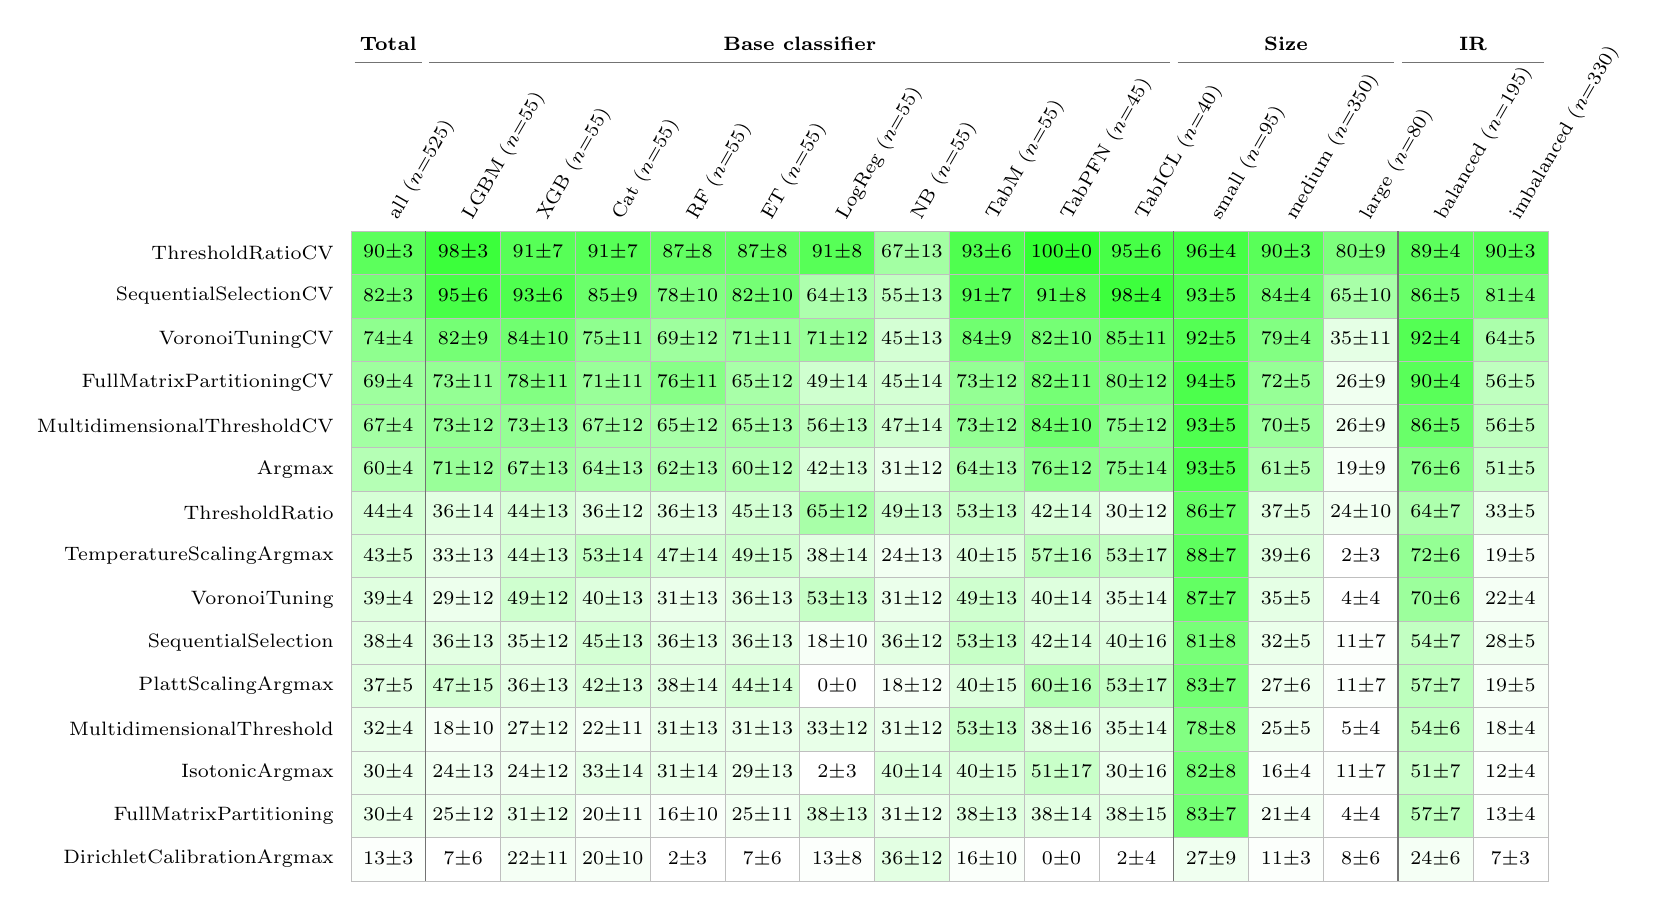
\begin{tikzpicture}[
    x=0.95cm, y=0.55cm,
    cell/.style={rectangle, draw=black!25, line width=0.2pt,
        minimum width=0.95cm, minimum height=0.55cm,
        anchor=center, font=\scriptsize, inner sep=0pt},
    rowlbl/.style={font=\scriptsize, anchor=east},
    collbl/.style={font=\scriptsize, anchor=west, rotate=60},
    grouplbl/.style={font=\scriptsize\bfseries, anchor=south},
    sep/.style={draw=black!55, line width=0.5pt},
]
\node[cell, fill=green!64] at (1, 15) {$90{\pm}3$};
\node[cell, fill=green!77] at (2, 15) {$98{\pm}3$};
\node[cell, fill=green!66] at (3, 15) {$91{\pm}7$};
\node[cell, fill=green!66] at (4, 15) {$91{\pm}7$};
\node[cell, fill=green!61] at (5, 15) {$87{\pm}8$};
\node[cell, fill=green!61] at (6, 15) {$87{\pm}8$};
\node[cell, fill=green!66] at (7, 15) {$91{\pm}8$};
\node[cell, fill=green!36] at (8, 15) {$67{\pm}13$};
\node[cell, fill=green!69] at (9, 15) {$93{\pm}6$};
\node[cell, fill=green!80] at (10, 15) {$100{\pm}0$};
\node[cell, fill=green!72] at (11, 15) {$95{\pm}6$};
\node[cell, fill=green!73] at (12, 15) {$96{\pm}4$};
\node[cell, fill=green!65] at (13, 15) {$90{\pm}3$};
\node[cell, fill=green!51] at (14, 15) {$80{\pm}9$};
\node[cell, fill=green!64] at (15, 15) {$89{\pm}4$};
\node[cell, fill=green!65] at (16, 15) {$90{\pm}3$};
\node[cell, fill=green!54] at (1, 14) {$82{\pm}3$};
\node[cell, fill=green!72] at (2, 14) {$95{\pm}6$};
\node[cell, fill=green!69] at (3, 14) {$93{\pm}6$};
\node[cell, fill=green!58] at (4, 14) {$85{\pm}9$};
\node[cell, fill=green!49] at (5, 14) {$78{\pm}10$};
\node[cell, fill=green!54] at (6, 14) {$82{\pm}10$};
\node[cell, fill=green!32] at (7, 14) {$64{\pm}13$};
\node[cell, fill=green!24] at (8, 14) {$55{\pm}13$};
\node[cell, fill=green!66] at (9, 14) {$91{\pm}7$};
\node[cell, fill=green!66] at (10, 14) {$91{\pm}8$};
\node[cell, fill=green!76] at (11, 14) {$98{\pm}4$};
\node[cell, fill=green!69] at (12, 14) {$93{\pm}5$};
\node[cell, fill=green!56] at (13, 14) {$84{\pm}4$};
\node[cell, fill=green!34] at (14, 14) {$65{\pm}10$};
\node[cell, fill=green!59] at (15, 14) {$86{\pm}5$};
\node[cell, fill=green!52] at (16, 14) {$81{\pm}4$};
\node[cell, fill=green!44] at (1, 13) {$74{\pm}4$};
\node[cell, fill=green!54] at (2, 13) {$82{\pm}9$};
\node[cell, fill=green!56] at (3, 13) {$84{\pm}10$};
\node[cell, fill=green!44] at (4, 13) {$75{\pm}11$};
\node[cell, fill=green!38] at (5, 13) {$69{\pm}12$};
\node[cell, fill=green!40] at (6, 13) {$71{\pm}11$};
\node[cell, fill=green!40] at (7, 13) {$71{\pm}12$};
\node[cell, fill=green!17] at (8, 13) {$45{\pm}13$};
\node[cell, fill=green!56] at (9, 13) {$84{\pm}9$};
\node[cell, fill=green!54] at (10, 13) {$82{\pm}10$};
\node[cell, fill=green!58] at (11, 13) {$85{\pm}11$};
\node[cell, fill=green!67] at (12, 13) {$92{\pm}5$};
\node[cell, fill=green!49] at (13, 13) {$79{\pm}4$};
\node[cell, fill=green!10] at (14, 13) {$35{\pm}11$};
\node[cell, fill=green!67] at (15, 13) {$92{\pm}4$};
\node[cell, fill=green!33] at (16, 13) {$64{\pm}5$};
\node[cell, fill=green!38] at (1, 12) {$69{\pm}4$};
\node[cell, fill=green!42] at (2, 12) {$73{\pm}11$};
\node[cell, fill=green!49] at (3, 12) {$78{\pm}11$};
\node[cell, fill=green!40] at (4, 12) {$71{\pm}11$};
\node[cell, fill=green!47] at (5, 12) {$76{\pm}11$};
\node[cell, fill=green!34] at (6, 12) {$65{\pm}12$};
\node[cell, fill=green!19] at (7, 12) {$49{\pm}14$};
\node[cell, fill=green!17] at (8, 12) {$45{\pm}14$};
\node[cell, fill=green!42] at (9, 12) {$73{\pm}12$};
\node[cell, fill=green!54] at (10, 12) {$82{\pm}11$};
\node[cell, fill=green!51] at (11, 12) {$80{\pm}12$};
\node[cell, fill=green!70] at (12, 12) {$94{\pm}5$};
\node[cell, fill=green!41] at (13, 12) {$72{\pm}5$};
\node[cell, fill=green!6] at (14, 12) {$26{\pm}9$};
\node[cell, fill=green!65] at (15, 12) {$90{\pm}4$};
\node[cell, fill=green!25] at (16, 12) {$56{\pm}5$};
\node[cell, fill=green!36] at (1, 11) {$67{\pm}4$};
\node[cell, fill=green!42] at (2, 11) {$73{\pm}12$};
\node[cell, fill=green!42] at (3, 11) {$73{\pm}13$};
\node[cell, fill=green!36] at (4, 11) {$67{\pm}12$};
\node[cell, fill=green!34] at (5, 11) {$65{\pm}12$};
\node[cell, fill=green!34] at (6, 11) {$65{\pm}13$};
\node[cell, fill=green!25] at (7, 11) {$56{\pm}13$};
\node[cell, fill=green!18] at (8, 11) {$47{\pm}14$};
\node[cell, fill=green!42] at (9, 11) {$73{\pm}12$};
\node[cell, fill=green!57] at (10, 11) {$84{\pm}10$};
\node[cell, fill=green!45] at (11, 11) {$75{\pm}12$};
\node[cell, fill=green!69] at (12, 11) {$93{\pm}5$};
\node[cell, fill=green!39] at (13, 11) {$70{\pm}5$};
\node[cell, fill=green!6] at (14, 11) {$26{\pm}9$};
\node[cell, fill=green!59] at (15, 11) {$86{\pm}5$};
\node[cell, fill=green!25] at (16, 11) {$56{\pm}5$};
\node[cell, fill=green!29] at (1, 10) {$60{\pm}4$};
\node[cell, fill=green!40] at (2, 10) {$71{\pm}12$};
\node[cell, fill=green!36] at (3, 10) {$67{\pm}13$};
\node[cell, fill=green!32] at (4, 10) {$64{\pm}13$};
\node[cell, fill=green!31] at (5, 10) {$62{\pm}13$};
\node[cell, fill=green!29] at (6, 10) {$60{\pm}12$};
\node[cell, fill=green!14] at (7, 10) {$42{\pm}13$};
\node[cell, fill=green!8] at (8, 10) {$31{\pm}12$};
\node[cell, fill=green!32] at (9, 10) {$64{\pm}13$};
\node[cell, fill=green!46] at (10, 10) {$76{\pm}12$};
\node[cell, fill=green!45] at (11, 10) {$75{\pm}14$};
\node[cell, fill=green!69] at (12, 10) {$93{\pm}5$};
\node[cell, fill=green!30] at (13, 10) {$61{\pm}5$};
\node[cell, fill=green!3] at (14, 10) {$19{\pm}9$};
\node[cell, fill=green!47] at (15, 10) {$76{\pm}6$};
\node[cell, fill=green!21] at (16, 10) {$51{\pm}5$};
\node[cell, fill=green!16] at (1, 9) {$44{\pm}4$};
\node[cell, fill=green!11] at (2, 9) {$36{\pm}14$};
\node[cell, fill=green!15] at (3, 9) {$44{\pm}13$};
\node[cell, fill=green!11] at (4, 9) {$36{\pm}12$};
\node[cell, fill=green!11] at (5, 9) {$36{\pm}13$};
\node[cell, fill=green!17] at (6, 9) {$45{\pm}13$};
\node[cell, fill=green!34] at (7, 9) {$65{\pm}12$};
\node[cell, fill=green!19] at (8, 9) {$49{\pm}13$};
\node[cell, fill=green!22] at (9, 9) {$53{\pm}13$};
\node[cell, fill=green!14] at (10, 9) {$42{\pm}14$};
\node[cell, fill=green!7] at (11, 9) {$30{\pm}12$};
\node[cell, fill=green!60] at (12, 9) {$86{\pm}7$};
\node[cell, fill=green!11] at (13, 9) {$37{\pm}5$};
\node[cell, fill=green!5] at (14, 9) {$24{\pm}10$};
\node[cell, fill=green!32] at (15, 9) {$64{\pm}7$};
\node[cell, fill=green!9] at (16, 9) {$33{\pm}5$};
\node[cell, fill=green!15] at (1, 8) {$43{\pm}5$};
\node[cell, fill=green!9] at (2, 8) {$33{\pm}13$};
\node[cell, fill=green!16] at (3, 8) {$44{\pm}13$};
\node[cell, fill=green!23] at (4, 8) {$53{\pm}14$};
\node[cell, fill=green!17] at (5, 8) {$47{\pm}14$};
\node[cell, fill=green!19] at (6, 8) {$49{\pm}15$};
\node[cell, fill=green!11] at (7, 8) {$38{\pm}14$};
\node[cell, fill=green!5] at (8, 8) {$24{\pm}13$};
\node[cell, fill=green!13] at (9, 8) {$40{\pm}15$};
\node[cell, fill=green!26] at (10, 8) {$57{\pm}16$};
\node[cell, fill=green!23] at (11, 8) {$53{\pm}17$};
\node[cell, fill=green!63] at (12, 8) {$88{\pm}7$};
\node[cell, fill=green!12] at (13, 8) {$39{\pm}6$};
\node[cell, fill=green!0] at (14, 8) {$2{\pm}3$};
\node[cell, fill=green!42] at (15, 8) {$72{\pm}6$};
\node[cell, fill=green!3] at (16, 8) {$19{\pm}5$};
\node[cell, fill=green!12] at (1, 7) {$39{\pm}4$};
\node[cell, fill=green!7] at (2, 7) {$29{\pm}12$};
\node[cell, fill=green!19] at (3, 7) {$49{\pm}12$};
\node[cell, fill=green!13] at (4, 7) {$40{\pm}13$};
\node[cell, fill=green!8] at (5, 7) {$31{\pm}13$};
\node[cell, fill=green!11] at (6, 7) {$36{\pm}13$};
\node[cell, fill=green!22] at (7, 7) {$53{\pm}13$};
\node[cell, fill=green!8] at (8, 7) {$31{\pm}12$};
\node[cell, fill=green!19] at (9, 7) {$49{\pm}13$};
\node[cell, fill=green!13] at (10, 7) {$40{\pm}14$};
\node[cell, fill=green!10] at (11, 7) {$35{\pm}14$};
\node[cell, fill=green!61] at (12, 7) {$87{\pm}7$};
\node[cell, fill=green!10] at (13, 7) {$35{\pm}5$};
\node[cell, fill=green!0] at (14, 7) {$4{\pm}4$};
\node[cell, fill=green!39] at (15, 7) {$70{\pm}6$};
\node[cell, fill=green!4] at (16, 7) {$22{\pm}4$};
\node[cell, fill=green!11] at (1, 6) {$38{\pm}4$};
\node[cell, fill=green!11] at (2, 6) {$36{\pm}13$};
\node[cell, fill=green!10] at (3, 6) {$35{\pm}12$};
\node[cell, fill=green!17] at (4, 6) {$45{\pm}13$};
\node[cell, fill=green!11] at (5, 6) {$36{\pm}13$};
\node[cell, fill=green!11] at (6, 6) {$36{\pm}13$};
\node[cell, fill=green!3] at (7, 6) {$18{\pm}10$};
\node[cell, fill=green!11] at (8, 6) {$36{\pm}12$};
\node[cell, fill=green!22] at (9, 6) {$53{\pm}13$};
\node[cell, fill=green!14] at (10, 6) {$42{\pm}14$};
\node[cell, fill=green!13] at (11, 6) {$40{\pm}16$};
\node[cell, fill=green!53] at (12, 6) {$81{\pm}8$};
\node[cell, fill=green!8] at (13, 6) {$32{\pm}5$};
\node[cell, fill=green!1] at (14, 6) {$11{\pm}7$};
\node[cell, fill=green!24] at (15, 6) {$54{\pm}7$};
\node[cell, fill=green!6] at (16, 6) {$28{\pm}5$};
\node[cell, fill=green!11] at (1, 5) {$37{\pm}5$};
\node[cell, fill=green!17] at (2, 5) {$47{\pm}15$};
\node[cell, fill=green!10] at (3, 5) {$36{\pm}13$};
\node[cell, fill=green!14] at (4, 5) {$42{\pm}13$};
\node[cell, fill=green!11] at (5, 5) {$38{\pm}14$};
\node[cell, fill=green!16] at (6, 5) {$44{\pm}14$};
\node[cell, fill=green!0] at (7, 5) {$0{\pm}0$};
\node[cell, fill=green!3] at (8, 5) {$18{\pm}12$};
\node[cell, fill=green!13] at (9, 5) {$40{\pm}15$};
\node[cell, fill=green!29] at (10, 5) {$60{\pm}16$};
\node[cell, fill=green!23] at (11, 5) {$53{\pm}17$};
\node[cell, fill=green!55] at (12, 5) {$83{\pm}7$};
\node[cell, fill=green!6] at (13, 5) {$27{\pm}6$};
\node[cell, fill=green!1] at (14, 5) {$11{\pm}7$};
\node[cell, fill=green!26] at (15, 5) {$57{\pm}7$};
\node[cell, fill=green!3] at (16, 5) {$19{\pm}5$};
\node[cell, fill=green!8] at (1, 4) {$32{\pm}4$};
\node[cell, fill=green!3] at (2, 4) {$18{\pm}10$};
\node[cell, fill=green!6] at (3, 4) {$27{\pm}12$};
\node[cell, fill=green!4] at (4, 4) {$22{\pm}11$};
\node[cell, fill=green!8] at (5, 4) {$31{\pm}13$};
\node[cell, fill=green!8] at (6, 4) {$31{\pm}13$};
\node[cell, fill=green!9] at (7, 4) {$33{\pm}12$};
\node[cell, fill=green!8] at (8, 4) {$31{\pm}12$};
\node[cell, fill=green!22] at (9, 4) {$53{\pm}13$};
\node[cell, fill=green!11] at (10, 4) {$38{\pm}16$};
\node[cell, fill=green!10] at (11, 4) {$35{\pm}14$};
\node[cell, fill=green!49] at (12, 4) {$78{\pm}8$};
\node[cell, fill=green!5] at (13, 4) {$25{\pm}5$};
\node[cell, fill=green!0] at (14, 4) {$5{\pm}4$};
\node[cell, fill=green!24] at (15, 4) {$54{\pm}6$};
\node[cell, fill=green!3] at (16, 4) {$18{\pm}4$};
\node[cell, fill=green!7] at (1, 3) {$30{\pm}4$};
\node[cell, fill=green!5] at (2, 3) {$24{\pm}13$};
\node[cell, fill=green!5] at (3, 3) {$24{\pm}12$};
\node[cell, fill=green!9] at (4, 3) {$33{\pm}14$};
\node[cell, fill=green!8] at (5, 3) {$31{\pm}14$};
\node[cell, fill=green!7] at (6, 3) {$29{\pm}13$};
\node[cell, fill=green!0] at (7, 3) {$2{\pm}3$};
\node[cell, fill=green!13] at (8, 3) {$40{\pm}14$};
\node[cell, fill=green!13] at (9, 3) {$40{\pm}15$};
\node[cell, fill=green!21] at (10, 3) {$51{\pm}17$};
\node[cell, fill=green!7] at (11, 3) {$30{\pm}16$};
\node[cell, fill=green!54] at (12, 3) {$82{\pm}8$};
\node[cell, fill=green!2] at (13, 3) {$16{\pm}4$};
\node[cell, fill=green!1] at (14, 3) {$11{\pm}7$};
\node[cell, fill=green!21] at (15, 3) {$51{\pm}7$};
\node[cell, fill=green!1] at (16, 3) {$12{\pm}4$};
\node[cell, fill=green!7] at (1, 2) {$30{\pm}4$};
\node[cell, fill=green!5] at (2, 2) {$25{\pm}12$};
\node[cell, fill=green!8] at (3, 2) {$31{\pm}12$};
\node[cell, fill=green!3] at (4, 2) {$20{\pm}11$};
\node[cell, fill=green!2] at (5, 2) {$16{\pm}10$};
\node[cell, fill=green!5] at (6, 2) {$25{\pm}11$};
\node[cell, fill=green!12] at (7, 2) {$38{\pm}13$};
\node[cell, fill=green!8] at (8, 2) {$31{\pm}12$};
\node[cell, fill=green!12] at (9, 2) {$38{\pm}13$};
\node[cell, fill=green!11] at (10, 2) {$38{\pm}14$};
\node[cell, fill=green!11] at (11, 2) {$38{\pm}15$};
\node[cell, fill=green!55] at (12, 2) {$83{\pm}7$};
\node[cell, fill=green!4] at (13, 2) {$21{\pm}4$};
\node[cell, fill=green!0] at (14, 2) {$4{\pm}4$};
\node[cell, fill=green!26] at (15, 2) {$57{\pm}7$};
\node[cell, fill=green!1] at (16, 2) {$13{\pm}4$};
\node[cell, fill=green!1] at (1, 1) {$13{\pm}3$};
\node[cell, fill=green!0] at (2, 1) {$7{\pm}6$};
\node[cell, fill=green!4] at (3, 1) {$22{\pm}11$};
\node[cell, fill=green!3] at (4, 1) {$20{\pm}10$};
\node[cell, fill=green!0] at (5, 1) {$2{\pm}3$};
\node[cell, fill=green!0] at (6, 1) {$7{\pm}6$};
\node[cell, fill=green!1] at (7, 1) {$13{\pm}8$};
\node[cell, fill=green!11] at (8, 1) {$36{\pm}12$};
\node[cell, fill=green!2] at (9, 1) {$16{\pm}10$};
\node[cell, fill=green!0] at (10, 1) {$0{\pm}0$};
\node[cell, fill=green!0] at (11, 1) {$2{\pm}4$};
\node[cell, fill=green!6] at (12, 1) {$27{\pm}9$};
\node[cell, fill=green!1] at (13, 1) {$11{\pm}3$};
\node[cell, fill=green!0] at (14, 1) {$8{\pm}6$};
\node[cell, fill=green!4] at (15, 1) {$24{\pm}6$};
\node[cell, fill=green!0] at (16, 1) {$7{\pm}3$};
\node[rowlbl] at (0.4, 15) {ThresholdRatioCV};
\node[rowlbl] at (0.4, 14) {SequentialSelectionCV};
\node[rowlbl] at (0.4, 13) {VoronoiTuningCV};
\node[rowlbl] at (0.4, 12) {FullMatrixPartitioningCV};
\node[rowlbl] at (0.4, 11) {MultidimensionalThresholdCV};
\node[rowlbl] at (0.4, 10) {Argmax};
\node[rowlbl] at (0.4, 9) {ThresholdRatio};
\node[rowlbl] at (0.4, 8) {TemperatureScalingArgmax};
\node[rowlbl] at (0.4, 7) {VoronoiTuning};
\node[rowlbl] at (0.4, 6) {SequentialSelection};
\node[rowlbl] at (0.4, 5) {PlattScalingArgmax};
\node[rowlbl] at (0.4, 4) {MultidimensionalThreshold};
\node[rowlbl] at (0.4, 3) {IsotonicArgmax};
\node[rowlbl] at (0.4, 2) {FullMatrixPartitioning};
\node[rowlbl] at (0.4, 1) {DirichletCalibrationArgmax};
\node[collbl] at (1, 15.6) {all ($n{=}525$)};
\node[collbl] at (2, 15.6) {LGBM ($n{=}55$)};
\node[collbl] at (3, 15.6) {XGB ($n{=}55$)};
\node[collbl] at (4, 15.6) {Cat ($n{=}55$)};
\node[collbl] at (5, 15.6) {RF ($n{=}55$)};
\node[collbl] at (6, 15.6) {ET ($n{=}55$)};
\node[collbl] at (7, 15.6) {LogReg ($n{=}55$)};
\node[collbl] at (8, 15.6) {NB ($n{=}55$)};
\node[collbl] at (9, 15.6) {TabM ($n{=}55$)};
\node[collbl] at (10, 15.6) {TabPFN ($n{=}45$)};
\node[collbl] at (11, 15.6) {TabICL ($n{=}40$)};
\node[collbl] at (12, 15.6) {small ($n{=}95$)};
\node[collbl] at (13, 15.6) {medium ($n{=}350$)};
\node[collbl] at (14, 15.6) {large ($n{=}80$)};
\node[collbl] at (15, 15.6) {balanced ($n{=}195$)};
\node[collbl] at (16, 15.6) {imbalanced ($n{=}330$)};
\draw[black!55, line width=0.5pt] (0.55, 19.4) -- (1.45, 19.4);
\node[grouplbl] at (1.0, 19.45) {Total};
\draw[black!55, line width=0.5pt] (1.55, 19.4) -- (11.45, 19.4);
\node[grouplbl] at (6.5, 19.45) {Base classifier};
\draw[black!55, line width=0.5pt] (11.55, 19.4) -- (14.45, 19.4);
\node[grouplbl] at (13.0, 19.45) {Size};
\draw[black!55, line width=0.5pt] (14.55, 19.4) -- (16.45, 19.4);
\node[grouplbl] at (15.5, 19.45) {IR};
\draw[sep] (1.5, 0.5) -- (1.5, 15.5);
\draw[sep] (11.5, 0.5) -- (11.5, 15.5);
\draw[sep] (14.5, 0.5) -- (14.5, 15.5);
\end{tikzpicture}%
}
\caption{Per-strategy win/tie rates on multiclass maximization metrics. Each cell reads ``$r{\pm}H$'': $r$ is the percentage of (dataset, model, objective) cells in the slice where the strategy won or tied the per-row best under the $\pm 1$ SE overlap rule, and $H$ is the half-width of a 95\% cluster-bootstrap confidence interval for $r$ (percentage points). Shading is a quadratic ($\mathrm{rate}^2$) scale of $r$. Strategies are sorted by overall win rate; ``$n$'' under each column header is the maximum applicable cell count for that slice.}%
\label{fig:win-counts-multiclass-max}
\end{figure}


\section{Summary of multiclass analysis}

The multiclass campaign supports three conclusions.

\begin{enumerate}
    \item The cross-validated tuning variants lead the per-row comparison on both objective groups. On cost objectives three variants share the top within sampling noise: FullMatrixPartitioningCV ($80\%$), RiskPartitioningCV ($79\%$), LinearScalingCV ($78\%$). On maximization metrics ThresholdRatioCV leads at $90\%$.
    \item The calibrate-then-analytical pipelines do not match the leading CV variants on cost (their win-or-tie rates are $30$ to $53\%$). The calibrators are fit on the $10\%$ validation partition while the CV variants use the full $80\%$ pool, so this gap is consistent with a label-budget gap but does not isolate it from other differences.
    \item The richer Voronoi class does not improve on the vector-tuned variants on this benchmark. Counting cells where a Voronoi variant is the unique SE-overlap winning family, the rate is $0.1\%$ on cost cells and $1.2\%$ on maximization cells. This is consistent with the population-level containment of Proposition~\ref{prop:ps_in_vor}: the strict advantage of Theorem~\ref{thm:rotational_dominance} requires a rotational regime the OpenML pool does not appear to concentrate in.
\end{enumerate}

%!TeX root=../carlo_master.tex
\chapter{Sensitivity to estimation misspecification across K}\label{sec:misspec_sensitivity_K}

The binary and multiclass campaigns of Sections~\ref{sec:binary_experiments} and~\ref{sec:multiclass_experiments} differ on a secondary observation. On cost-matrix objectives, the lead in overall win/tie rate of the best strategy over the bare analytical plug-in rule narrows from $87\%$ versus $69\%$ in the binary setting (Figure~\ref{fig:win-counts-binary-cost}) to $80\%$ versus $69\%$ in the multiclass setting (Figure~\ref{fig:win-counts-multiclass-cost}), i.e.\ from an $18$-point lead to an $11$-point lead. On the non-decomposable maximization metrics, where the analytical rule reduces to argmax-of-probabilities, the comparison narrows from $100\%$ versus $45\%$ (Figure~\ref{fig:win-counts-binary-max}) to $90\%$ versus $62\%$ (Figure~\ref{fig:win-counts-multiclass-max}). The direction is consistent across both objective families: the lead of the best strategy over the analytical rule shrinks as $K$ grows.

There are two candidate explanations. Either the multiclass validation partition carries little exploitable signal, or the analytical Bayes-optimal rule itself becomes more robust to distributional misspecification as $K$ grows. We test the second reading with two controlled synthetic experiments and propose a candidate mechanism for it.

\section{Synthetic experiments}\label{sec:misspec_sensitivity_experiments}

Both experiments use closed-form Gaussian class-conditional densities and evaluate the analytical Bayes-optimal rule directly under the perturbed distribution; Monte Carlo enters only to evaluate expectations. They differ in the perturbation: variance scaling (Section~\ref{sec:misspec_sensitivity_variance}) is observable only under an asymmetric cost, while per-class random mean shifts (Section~\ref{sec:misspec_sensitivity_meanshift}) break the argmax-invariance and reproduce the K-monotone ordering under both symmetric and asymmetric cost.

\subsection{Variance scaling}\label{sec:misspec_sensitivity_variance}

Let $\mathbb{P}_1$ denote the reference distribution over $(X, Y) \in \mathbb{R}^2 \times \mathcal{Y}$ in which the class priors are uniform ($\pi_k = 1/K$) and each class-conditional density is isotropic Gaussian, $p_1(x \mid Y{=}k) = \mathcal{N}(\mathbf{m}_k, \sigma^2 \mathbf{I})$ with $\sigma = 1$; it is the identity member of the variance family $\{\mathbb{P}_\lambda\}_{\lambda \geq 1}$ defined next. The feature-space class means $\mathbf{m}_k \in \mathbb{R}^2$ are placed at the vertices of a regular $K$-gon of radius $2$, so the geometric arrangement is rotationally symmetric; at this fixed radius the distance between adjacent class means, $4\sin(\pi/K)$, decreases as $K$ grows.

The misspecified member $\mathbb{P}_\lambda$ shares the means and priors of $\mathbb{P}_1$ but scales every class-conditional density to $p_\lambda(x \mid Y{=}k) = \mathcal{N}(\mathbf{m}_k, \lambda\sigma^2 \mathbf{I})$ for a single variance multiplier $\lambda \geq 1$, with the reference recovered at the identity value $\lambda = 1$. Write $\boldsymbol{\eta}_1(x)$ and $\boldsymbol{\eta}_\lambda(x)$ for the conditional class probabilities induced by $\mathbb{P}_1$ and $\mathbb{P}_\lambda$ at $x$. Here $\boldsymbol{\eta}_1$ plays the role of the misspecified plug-in estimate $\hat{\mathbf{p}}$ and $\boldsymbol{\eta}_\lambda$ the role of the truth $\boldsymbol{\eta}$, so the difference $\boldsymbol{\eta}_\lambda - \boldsymbol{\eta}_1$ is the estimation error $\boldsymbol{\epsilon}$ of Section~\ref{sec:analytical_fragility}.

The misspecified rule applies the Bayes-optimal decision $\delta^*$ from~\eqref{eq:bayes_optimal_delta} to $\boldsymbol{\eta}_1(x)$, equivalent to assuming the variance is $\sigma^2$, while the oracle applies the same $\delta^*$ to $\boldsymbol{\eta}_\lambda(x)$. Figure~\ref{fig:misspec-sensitivity-setup-geometry} illustrates the construction at $K = 5$: the assumed unit-variance contours sit inside the larger contours of $\mathbb{P}_\lambda$, and the misspecified rule built for the inner geometry is asked to act on data drawn from the outer one.

\begin{figure}[H]
    \centering
    \documentclass[tikz, border=10pt]{standalone}
\usepackage{tikz}
\usepackage{amsmath}
\usetikzlibrary{calc}

\begin{document}
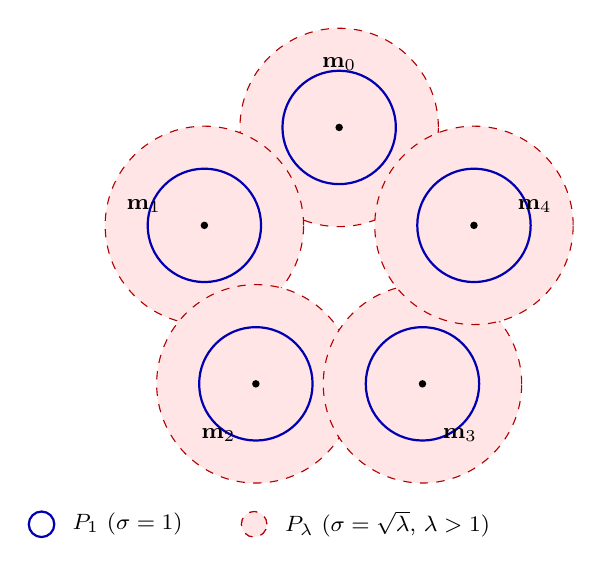
\begin{tikzpicture}[font=\sffamily, scale=0.9]

    % K = 5 class means on a regular K-gon of radius r = 2. mu_0 sits
    % at the top (angle 90 deg); the remaining four vertices are spaced
    % 72 deg apart going counter-clockwise.
    \def\sep{2}
    \def\sigP{0.8}
    \def\sigQ{1.4}

    % Q variance contours, drawn first so the P0 rings sit on top.
    \foreach \i in {0,1,2,3,4} {
        \pgfmathsetmacro{\angle}{90 + 72 * \i}
        \pgfmathsetmacro{\xc}{\sep*cos(\angle)}
        \pgfmathsetmacro{\yc}{\sep*sin(\angle)}
        \fill[red!10] (\xc,\yc) circle (\sigQ);
        \draw[red!70!black, dashed, thin] (\xc,\yc) circle (\sigQ);
    }

    % P0 variance contours plus class-mean dots.
    \foreach \i in {0,1,2,3,4} {
        \pgfmathsetmacro{\angle}{90 + 72 * \i}
        \pgfmathsetmacro{\xc}{\sep*cos(\angle)}
        \pgfmathsetmacro{\yc}{\sep*sin(\angle)}
        \draw[blue!70!black, thick] (\xc,\yc) circle (\sigP);
        \fill[black] (\xc,\yc) circle (1.5pt);
        \pgfmathsetmacro{\lxc}{1.45*\xc}
        \pgfmathsetmacro{\lyc}{1.45*\yc}
        \node[font=\footnotesize] at (\lxc,\lyc) {$\mathbf{m}_{\i}$};
    }

    % Legend.
    \begin{scope}[shift={(-4.2, -3.6)}, font=\footnotesize]
        \draw[blue!70!black, thick] (0,0) circle (0.18);
        \node[anchor=west] at (0.3, 0) {$\mathbb{P}_1$ ($\sigma = 1$)};
        \draw[red!70!black, dashed, thin] (3.0, 0) circle (0.18);
        \fill[red!10] (3.0, 0) circle (0.18);
        \draw[red!70!black, dashed, thin] (3.0, 0) circle (0.18);
        \node[anchor=west] at (3.3, 0) {$\mathbb{P}_\lambda$ ($\sigma = \sqrt{\lambda}$, $\lambda > 1$)};
    \end{scope}

\end{tikzpicture}
\end{document}

    \caption{Variance-scaling perturbation at $K = 5$ in $\mathbb{R}^2$. The class means $\mathbf{m}_k$ sit at the vertices of a regular $K$-gon of radius $2$. Solid blue rings show the $\mathbb{P}_1$ contours at $\sigma = 1$; faded red rings show $\mathbb{P}_\lambda$ contours at $\sigma = \sqrt{\lambda}$ for an example $\lambda > 1$ (here $\lambda \approx 3$). The misspecified rule is built for the inner geometry and applied to data sampled from the outer one.}%
    \label{fig:misspec-sensitivity-setup-geometry}
\end{figure}

The variance multiplier $\lambda$ is the construction's K-independent sweep parameter, so the per-$K$ curves share a common horizontal axis: the per-class KL divergence between $\mathbb{P}_1$ and $\mathbb{P}_\lambda$ equals $(d/2)(\log\lambda + 1/\lambda - 1)$ with $d = 2$, independent of $K$ (Appendix~\ref{app:kl_invariance}). We sweep $17$ log-spaced values of $\lambda$ in $[1, 16]$.

The cost matrix $\mathbf{C}$ is the Asymmetric $10\times$ family from Section~\ref{sec:multiclass_setup}: class $K{-}1$ is designated high-cost so that misclassifying it carries cost $10$, while every other off-diagonal misclassification carries cost $1$. Writing $R_\lambda(h) = \mathbb{E}_{\mathbb{P}_\lambda}[C_{Y, h(X)}]$ for the expected risk of a classifier $h$ under $\mathbb{P}_\lambda$, the oracle classifier is $h^*_\lambda(x) = \delta^*(\boldsymbol{\eta}_\lambda(x))$ and the misspecified classifier is $h^*_1(x) = \delta^*(\boldsymbol{\eta}_1(x))$. We report the relative excess risk,
\begin{equation}
    \frac{R_\lambda(h^*_1) - R_\lambda(h^*_\lambda)}{R_\lambda(h^*_\lambda)},
    \label{eq:misspec_sensitivity_relative_regret}
\end{equation}
which normalises out the baseline difficulty of the cost matrix and is identically zero at $\lambda = 1$ (where the two classifiers coincide).

Expectations are estimated by stratified Monte Carlo. Each task draws $n_{\mathrm{MC}} = 100{,}000$ samples from $\mathbb{P}_\lambda$, evaluates both classifiers on the same samples (shared-sample evaluation cancels most of the Monte Carlo variance in the difference, since the two classifiers agree at every $x$ that is not near a decision boundary), and records both risk estimates. The replicate seed vector is drawn deterministically from a master seed and persisted alongside the run, matching the protocol used by the mean-shift sweep of Section~\ref{sec:misspec_sensitivity_meanshift}. The sweep covers $K \in \{2, 3, 4, 5, 7, 10, 15, 20\}$; the lower endpoint $K = 2$ recovers the binary problem and serves as the bridge to Section~\ref{sec:binary_experiments}.

Figure~\ref{fig:misspec-sensitivity-variance} overlays the eight per-$K$ curves on a single panel. All curves anchor near zero and grow with $\lambda$. The ordering is monotone in $K$ across the bulk of the sweep: at every fixed $\lambda$ above the Monte Carlo floor the $K = 2$ curve sits highest, $K = 3$ next, and so on down to $K = 20$ at the bottom. Between $K = 2$ and $K = 20$ the relative excess risk differs by a factor of roughly seven to eight across $\lambda \in [1, 16]$.

This K-monotone ordering of relative excess risk is the empirical phenomenon predicted qualitatively by the second reading of the section's opening; Section~\ref{sec:misspec_sensitivity_mechanism} proposes a candidate geometric mechanism for it.

\begin{figure}[H]
    \centering
    % Auto-generated by experiments.analysis.generate_variance_figure --- do not edit.
% Cost: Asymmetric 10x. Uniform variance perturbation across classes, lambda >= 1.
% Horizontal axis is the variance multiplier lambda.
% Left log-log, right linear; bands are normal-approx 95% CIs (mean +/- 1.96 * SE).
\noindent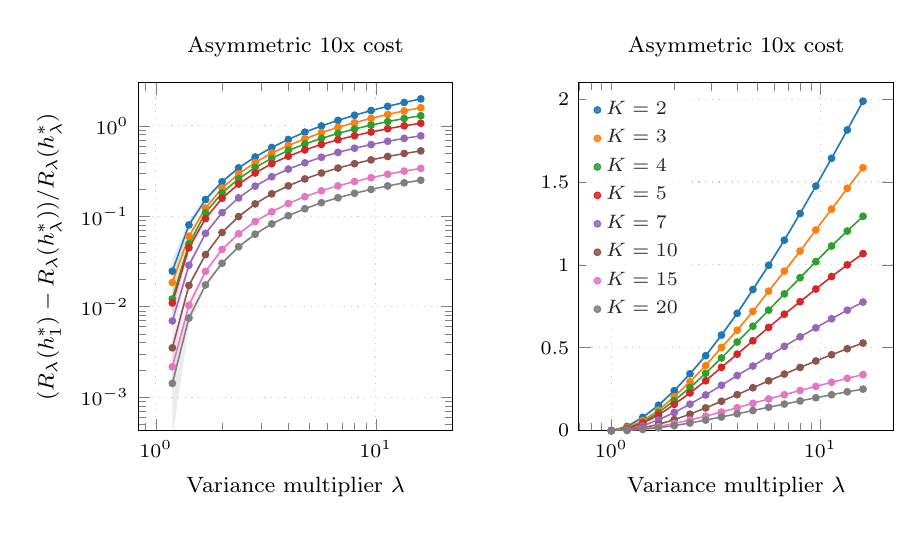
\begin{tikzpicture}
\begin{groupplot}[
    group style={group size=2 by 1, horizontal sep=1.6cm},
    width=0.46\textwidth, height=6.0cm,
    grid=major, grid style={dotted, gray!40},
    xmode=log,
    tick label style={font=\scriptsize},
    label style={font=\footnotesize},
    title style={font=\footnotesize},
]
\nextgroupplot[
    title={Asymmetric 10x cost},
    xlabel={Variance multiplier $\lambda$},
    ylabel={$(R_\lambda(h^{\ast}_1) - R_\lambda(h^{\ast}_\lambda)) / R_\lambda(h^{\ast}_\lambda)$},
    ymode=log,
    xmin=0.8323, xmax=22.4, ymin=0.000425688, ymax=2.99919,
]
\addplot[name path=lo_log_K2, draw=none, forget plot] coordinates {
        (1.189, 0.0161447)
        (1.414, 0.0718404)
        (1.682, 0.142239)
        (2, 0.231757)
        (2.378, 0.333251)
        (2.828, 0.441629)
        (3.364, 0.563046)
        (4, 0.692213)
        (4.757, 0.836961)
        (5.657, 0.98451)
        (6.727, 1.13795)
        (8, 1.29971)
        (9.514, 1.46486)
        (11.314, 1.6324)
        (13.454, 1.80237)
        (16, 1.97649)
    };
\addplot[name path=hi_log_K2, draw=none, forget plot] coordinates {
        (1.189, 0.0333247)
        (1.414, 0.0884253)
        (1.682, 0.163695)
        (2, 0.250187)
        (2.378, 0.352524)
        (2.828, 0.462834)
        (3.364, 0.589603)
        (4, 0.722949)
        (4.757, 0.865979)
        (5.657, 1.0107)
        (6.727, 1.16066)
        (8, 1.32026)
        (9.514, 1.48627)
        (11.314, 1.65422)
        (13.454, 1.82666)
        (16, 1.99946)
    };
\addplot[color={rgb,255:red,31; green,119; blue,180}, opacity=0.15, forget plot] fill between [of=lo_log_K2 and hi_log_K2];
\addplot[only marks, mark=*, mark size=1.2pt, color={rgb,255:red,31; green,119; blue,180}] coordinates {
        (1.189, 0.0247347)
        (1.414, 0.0801328)
        (1.682, 0.152967)
        (2, 0.240972)
        (2.378, 0.342888)
        (2.828, 0.452231)
        (3.364, 0.576325)
        (4, 0.707581)
        (4.757, 0.85147)
        (5.657, 0.997606)
        (6.727, 1.14931)
        (8, 1.30999)
        (9.514, 1.47557)
        (11.314, 1.64331)
        (13.454, 1.81451)
        (16, 1.98798)
    };
\addplot[color={rgb,255:red,31; green,119; blue,180}, line width=0.55pt, forget plot] coordinates {
        (1.189, 0.0247347)
        (1.414, 0.0801328)
        (1.682, 0.152967)
        (2, 0.240972)
        (2.378, 0.342888)
        (2.828, 0.452231)
        (3.364, 0.576325)
        (4, 0.707581)
        (4.757, 0.85147)
        (5.657, 0.997606)
        (6.727, 1.14931)
        (8, 1.30999)
        (9.514, 1.47557)
        (11.314, 1.64331)
        (13.454, 1.81451)
        (16, 1.98798)
    };
\addplot[name path=lo_log_K3, draw=none, forget plot] coordinates {
        (1.189, 0.0137686)
        (1.414, 0.0552877)
        (1.682, 0.115988)
        (2, 0.195324)
        (2.378, 0.286426)
        (2.828, 0.382433)
        (3.364, 0.490037)
        (4, 0.593463)
        (4.757, 0.708625)
        (5.657, 0.830985)
        (6.727, 0.952376)
        (8, 1.07403)
        (9.514, 1.20365)
        (11.314, 1.32945)
        (13.454, 1.45665)
        (16, 1.5818)
    };
\addplot[name path=hi_log_K3, draw=none, forget plot] coordinates {
        (1.189, 0.0232883)
        (1.414, 0.0648708)
        (1.682, 0.13004)
        (2, 0.214727)
        (2.378, 0.303447)
        (2.828, 0.40297)
        (3.364, 0.512568)
        (4, 0.618329)
        (4.757, 0.730788)
        (5.657, 0.852117)
        (6.727, 0.97242)
        (8, 1.0927)
        (9.514, 1.21752)
        (11.314, 1.34388)
        (13.454, 1.46793)
        (16, 1.59037)
    };
\addplot[color={rgb,255:red,255; green,127; blue,14}, opacity=0.15, forget plot] fill between [of=lo_log_K3 and hi_log_K3];
\addplot[only marks, mark=*, mark size=1.2pt, color={rgb,255:red,255; green,127; blue,14}] coordinates {
        (1.189, 0.0185285)
        (1.414, 0.0600792)
        (1.682, 0.123014)
        (2, 0.205025)
        (2.378, 0.294936)
        (2.828, 0.392701)
        (3.364, 0.501303)
        (4, 0.605896)
        (4.757, 0.719706)
        (5.657, 0.841551)
        (6.727, 0.962398)
        (8, 1.08336)
        (9.514, 1.21058)
        (11.314, 1.33667)
        (13.454, 1.46229)
        (16, 1.58608)
    };
\addplot[color={rgb,255:red,255; green,127; blue,14}, line width=0.55pt, forget plot] coordinates {
        (1.189, 0.0185285)
        (1.414, 0.0600792)
        (1.682, 0.123014)
        (2, 0.205025)
        (2.378, 0.294936)
        (2.828, 0.392701)
        (3.364, 0.501303)
        (4, 0.605896)
        (4.757, 0.719706)
        (5.657, 0.841551)
        (6.727, 0.962398)
        (8, 1.08336)
        (9.514, 1.21058)
        (11.314, 1.33667)
        (13.454, 1.46229)
        (16, 1.58608)
    };
\addplot[name path=lo_log_K4, draw=none, forget plot] coordinates {
        (1.189, 0.00786415)
        (1.414, 0.0468163)
        (1.682, 0.103907)
        (2, 0.175578)
        (2.378, 0.251519)
        (2.828, 0.339396)
        (3.364, 0.432449)
        (4, 0.526692)
        (4.757, 0.622574)
        (5.657, 0.719398)
        (6.727, 0.818424)
        (8, 0.916216)
        (9.514, 1.01238)
        (11.314, 1.10722)
        (13.454, 1.19747)
        (16, 1.28595)
    };
\addplot[name path=hi_log_K4, draw=none, forget plot] coordinates {
        (1.189, 0.0164744)
        (1.414, 0.0522307)
        (1.682, 0.114793)
        (2, 0.187296)
        (2.378, 0.266792)
        (2.828, 0.352795)
        (3.364, 0.443914)
        (4, 0.542168)
        (4.757, 0.637706)
        (5.657, 0.734813)
        (6.727, 0.831237)
        (8, 0.929232)
        (9.514, 1.02673)
        (11.314, 1.12098)
        (13.454, 1.21126)
        (16, 1.30044)
    };
\addplot[color={rgb,255:red,44; green,160; blue,44}, opacity=0.15, forget plot] fill between [of=lo_log_K4 and hi_log_K4];
\addplot[only marks, mark=*, mark size=1.2pt, color={rgb,255:red,44; green,160; blue,44}] coordinates {
        (1.189, 0.0121693)
        (1.414, 0.0495235)
        (1.682, 0.10935)
        (2, 0.181437)
        (2.378, 0.259155)
        (2.828, 0.346095)
        (3.364, 0.438182)
        (4, 0.53443)
        (4.757, 0.63014)
        (5.657, 0.727105)
        (6.727, 0.82483)
        (8, 0.922724)
        (9.514, 1.01956)
        (11.314, 1.1141)
        (13.454, 1.20437)
        (16, 1.29319)
    };
\addplot[color={rgb,255:red,44; green,160; blue,44}, line width=0.55pt, forget plot] coordinates {
        (1.189, 0.0121693)
        (1.414, 0.0495235)
        (1.682, 0.10935)
        (2, 0.181437)
        (2.378, 0.259155)
        (2.828, 0.346095)
        (3.364, 0.438182)
        (4, 0.53443)
        (4.757, 0.63014)
        (5.657, 0.727105)
        (6.727, 0.82483)
        (8, 0.922724)
        (9.514, 1.01956)
        (11.314, 1.1141)
        (13.454, 1.20437)
        (16, 1.29319)
    };
\addplot[name path=lo_log_K5, draw=none, forget plot] coordinates {
        (1.189, 0.00858714)
        (1.414, 0.0412982)
        (1.682, 0.0908124)
        (2, 0.153464)
        (2.378, 0.220724)
        (2.828, 0.296552)
        (3.364, 0.377461)
        (4, 0.457546)
        (4.757, 0.538286)
        (5.657, 0.618597)
        (6.727, 0.697442)
        (8, 0.773356)
        (9.514, 0.848852)
        (11.314, 0.924177)
        (13.454, 0.995903)
        (16, 1.06329)
    };
\addplot[name path=hi_log_K5, draw=none, forget plot] coordinates {
        (1.189, 0.0134082)
        (1.414, 0.0484077)
        (1.682, 0.0977084)
        (2, 0.163215)
        (2.378, 0.233467)
        (2.828, 0.305662)
        (3.364, 0.386235)
        (4, 0.465198)
        (4.757, 0.545995)
        (5.657, 0.62696)
        (6.727, 0.707023)
        (8, 0.782956)
        (9.514, 0.859622)
        (11.314, 0.934936)
        (13.454, 1.00517)
        (16, 1.07274)
    };
\addplot[color={rgb,255:red,214; green,39; blue,40}, opacity=0.15, forget plot] fill between [of=lo_log_K5 and hi_log_K5];
\addplot[only marks, mark=*, mark size=1.2pt, color={rgb,255:red,214; green,39; blue,40}] coordinates {
        (1.189, 0.0109977)
        (1.414, 0.044853)
        (1.682, 0.0942604)
        (2, 0.15834)
        (2.378, 0.227096)
        (2.828, 0.301107)
        (3.364, 0.381848)
        (4, 0.461372)
        (4.757, 0.54214)
        (5.657, 0.622778)
        (6.727, 0.702232)
        (8, 0.778156)
        (9.514, 0.854237)
        (11.314, 0.929557)
        (13.454, 1.00054)
        (16, 1.06801)
    };
\addplot[color={rgb,255:red,214; green,39; blue,40}, line width=0.55pt, forget plot] coordinates {
        (1.189, 0.0109977)
        (1.414, 0.044853)
        (1.682, 0.0942604)
        (2, 0.15834)
        (2.378, 0.227096)
        (2.828, 0.301107)
        (3.364, 0.381848)
        (4, 0.461372)
        (4.757, 0.54214)
        (5.657, 0.622778)
        (6.727, 0.702232)
        (8, 0.778156)
        (9.514, 0.854237)
        (11.314, 0.929557)
        (13.454, 1.00054)
        (16, 1.06801)
    };
\addplot[name path=lo_log_K7, draw=none, forget plot] coordinates {
        (1.189, 0.00489146)
        (1.414, 0.0256547)
        (1.682, 0.0620802)
        (2, 0.106804)
        (2.378, 0.156521)
        (2.828, 0.211665)
        (3.364, 0.270368)
        (4, 0.329369)
        (4.757, 0.385826)
        (5.657, 0.444772)
        (6.727, 0.505012)
        (8, 0.561215)
        (9.514, 0.616402)
        (11.314, 0.67075)
        (13.454, 0.723249)
        (16, 0.773113)
    };
\addplot[name path=hi_log_K7, draw=none, forget plot] coordinates {
        (1.189, 0.0090175)
        (1.414, 0.0318048)
        (1.682, 0.0671157)
        (2, 0.112398)
        (2.378, 0.162664)
        (2.828, 0.218827)
        (3.364, 0.276874)
        (4, 0.335041)
        (4.757, 0.393183)
        (5.657, 0.454228)
        (6.727, 0.51215)
        (8, 0.570211)
        (9.514, 0.623927)
        (11.314, 0.67861)
        (13.454, 0.730012)
        (16, 0.778521)
    };
\addplot[color={rgb,255:red,148; green,103; blue,189}, opacity=0.15, forget plot] fill between [of=lo_log_K7 and hi_log_K7];
\addplot[only marks, mark=*, mark size=1.2pt, color={rgb,255:red,148; green,103; blue,189}] coordinates {
        (1.189, 0.00695448)
        (1.414, 0.0287297)
        (1.682, 0.064598)
        (2, 0.109601)
        (2.378, 0.159592)
        (2.828, 0.215246)
        (3.364, 0.273621)
        (4, 0.332205)
        (4.757, 0.389504)
        (5.657, 0.4495)
        (6.727, 0.508581)
        (8, 0.565713)
        (9.514, 0.620165)
        (11.314, 0.67468)
        (13.454, 0.72663)
        (16, 0.775817)
    };
\addplot[color={rgb,255:red,148; green,103; blue,189}, line width=0.55pt, forget plot] coordinates {
        (1.189, 0.00695448)
        (1.414, 0.0287297)
        (1.682, 0.064598)
        (2, 0.109601)
        (2.378, 0.159592)
        (2.828, 0.215246)
        (3.364, 0.273621)
        (4, 0.332205)
        (4.757, 0.389504)
        (5.657, 0.4495)
        (6.727, 0.508581)
        (8, 0.565713)
        (9.514, 0.620165)
        (11.314, 0.67468)
        (13.454, 0.72663)
        (16, 0.775817)
    };
\addplot[name path=lo_log_K10, draw=none, forget plot] coordinates {
        (1.189, 0.00241518)
        (1.414, 0.0161753)
        (1.682, 0.0360415)
        (2, 0.0636871)
        (2.378, 0.0957237)
        (2.828, 0.133838)
        (3.364, 0.173433)
        (4, 0.214331)
        (4.757, 0.256292)
        (5.657, 0.298534)
        (6.727, 0.339362)
        (8, 0.379891)
        (9.514, 0.418268)
        (11.314, 0.455481)
        (13.454, 0.491666)
        (16, 0.526482)
    };
\addplot[name path=hi_log_K10, draw=none, forget plot] coordinates {
        (1.189, 0.00459898)
        (1.414, 0.0181741)
        (1.682, 0.0393009)
        (2, 0.0686597)
        (2.378, 0.102639)
        (2.828, 0.140313)
        (3.364, 0.180654)
        (4, 0.219588)
        (4.757, 0.260894)
        (5.657, 0.302297)
        (6.727, 0.342851)
        (8, 0.382769)
        (9.514, 0.422214)
        (11.314, 0.460574)
        (13.454, 0.496621)
        (16, 0.530226)
    };
\addplot[color={rgb,255:red,140; green,86; blue,75}, opacity=0.15, forget plot] fill between [of=lo_log_K10 and hi_log_K10];
\addplot[only marks, mark=*, mark size=1.2pt, color={rgb,255:red,140; green,86; blue,75}] coordinates {
        (1.189, 0.00350708)
        (1.414, 0.0171747)
        (1.682, 0.0376712)
        (2, 0.0661734)
        (2.378, 0.0991812)
        (2.828, 0.137075)
        (3.364, 0.177044)
        (4, 0.216959)
        (4.757, 0.258593)
        (5.657, 0.300416)
        (6.727, 0.341107)
        (8, 0.38133)
        (9.514, 0.420241)
        (11.314, 0.458028)
        (13.454, 0.494143)
        (16, 0.528354)
    };
\addplot[color={rgb,255:red,140; green,86; blue,75}, line width=0.55pt, forget plot] coordinates {
        (1.189, 0.00350708)
        (1.414, 0.0171747)
        (1.682, 0.0376712)
        (2, 0.0661734)
        (2.378, 0.0991812)
        (2.828, 0.137075)
        (3.364, 0.177044)
        (4, 0.216959)
        (4.757, 0.258593)
        (5.657, 0.300416)
        (6.727, 0.341107)
        (8, 0.38133)
        (9.514, 0.420241)
        (11.314, 0.458028)
        (13.454, 0.494143)
        (16, 0.528354)
    };
\addplot[name path=lo_log_K15, draw=none, forget plot] coordinates {
        (1.189, 0.001182)
        (1.414, 0.00862062)
        (1.682, 0.0232245)
        (2, 0.0412677)
        (2.378, 0.0615452)
        (2.828, 0.0847089)
        (3.364, 0.109374)
        (4, 0.135708)
        (4.757, 0.161873)
        (5.657, 0.189942)
        (6.727, 0.214806)
        (8, 0.23984)
        (9.514, 0.263725)
        (11.314, 0.28837)
        (13.454, 0.312157)
        (16, 0.335172)
    };
\addplot[name path=hi_log_K15, draw=none, forget plot] coordinates {
        (1.189, 0.00314398)
        (1.414, 0.012143)
        (1.682, 0.0258598)
        (2, 0.0446189)
        (2.378, 0.0664429)
        (2.828, 0.0901067)
        (3.364, 0.114541)
        (4, 0.140388)
        (4.757, 0.167171)
        (5.657, 0.192335)
        (6.727, 0.218389)
        (8, 0.244384)
        (9.514, 0.270009)
        (11.314, 0.29453)
        (13.454, 0.318543)
        (16, 0.340795)
    };
\addplot[color={rgb,255:red,227; green,119; blue,194}, opacity=0.15, forget plot] fill between [of=lo_log_K15 and hi_log_K15];
\addplot[only marks, mark=*, mark size=1.2pt, color={rgb,255:red,227; green,119; blue,194}] coordinates {
        (1.189, 0.00216299)
        (1.414, 0.0103818)
        (1.682, 0.0245422)
        (2, 0.0429433)
        (2.378, 0.0639941)
        (2.828, 0.0874078)
        (3.364, 0.111958)
        (4, 0.138048)
        (4.757, 0.164522)
        (5.657, 0.191139)
        (6.727, 0.216598)
        (8, 0.242112)
        (9.514, 0.266867)
        (11.314, 0.29145)
        (13.454, 0.31535)
        (16, 0.337984)
    };
\addplot[color={rgb,255:red,227; green,119; blue,194}, line width=0.55pt, forget plot] coordinates {
        (1.189, 0.00216299)
        (1.414, 0.0103818)
        (1.682, 0.0245422)
        (2, 0.0429433)
        (2.378, 0.0639941)
        (2.828, 0.0874078)
        (3.364, 0.111958)
        (4, 0.138048)
        (4.757, 0.164522)
        (5.657, 0.191139)
        (6.727, 0.216598)
        (8, 0.242112)
        (9.514, 0.266867)
        (11.314, 0.29145)
        (13.454, 0.31535)
        (16, 0.337984)
    };
\addplot[name path=lo_log_K20, draw=none, forget plot] coordinates {
        (1.189, 0.0003523)
        (1.414, 0.00614175)
        (1.682, 0.0162756)
        (2, 0.0286209)
        (2.378, 0.0437608)
        (2.828, 0.0615339)
        (3.364, 0.0802796)
        (4, 0.0996629)
        (4.757, 0.118941)
        (5.657, 0.139655)
        (6.727, 0.158926)
        (8, 0.177475)
        (9.514, 0.196231)
        (11.314, 0.21439)
        (13.454, 0.23227)
        (16, 0.248269)
    };
\addplot[name path=hi_log_K20, draw=none, forget plot] coordinates {
        (1.189, 0.00248562)
        (1.414, 0.00882633)
        (1.682, 0.0184819)
        (2, 0.0318147)
        (2.378, 0.0482381)
        (2.828, 0.0651807)
        (3.364, 0.0842073)
        (4, 0.103315)
        (4.757, 0.122889)
        (5.657, 0.142877)
        (6.727, 0.161536)
        (8, 0.181019)
        (9.514, 0.199929)
        (11.314, 0.218523)
        (13.454, 0.236528)
        (16, 0.252079)
    };
\addplot[color={rgb,255:red,127; green,127; blue,127}, opacity=0.15, forget plot] fill between [of=lo_log_K20 and hi_log_K20];
\addplot[only marks, mark=*, mark size=1.2pt, color={rgb,255:red,127; green,127; blue,127}] coordinates {
        (1.189, 0.00141896)
        (1.414, 0.00748404)
        (1.682, 0.0173788)
        (2, 0.0302178)
        (2.378, 0.0459995)
        (2.828, 0.0633573)
        (3.364, 0.0822435)
        (4, 0.101489)
        (4.757, 0.120915)
        (5.657, 0.141266)
        (6.727, 0.160231)
        (8, 0.179247)
        (9.514, 0.19808)
        (11.314, 0.216457)
        (13.454, 0.234399)
        (16, 0.250174)
    };
\addplot[color={rgb,255:red,127; green,127; blue,127}, line width=0.55pt, forget plot] coordinates {
        (1.189, 0.00141896)
        (1.414, 0.00748404)
        (1.682, 0.0173788)
        (2, 0.0302178)
        (2.378, 0.0459995)
        (2.828, 0.0633573)
        (3.364, 0.0822435)
        (4, 0.101489)
        (4.757, 0.120915)
        (5.657, 0.141266)
        (6.727, 0.160231)
        (8, 0.179247)
        (9.514, 0.19808)
        (11.314, 0.216457)
        (13.454, 0.234399)
        (16, 0.250174)
    };
\nextgroupplot[
    title={Asymmetric 10x cost},
    xlabel={Variance multiplier $\lambda$},
    ymode=normal,
    legend style={font=\scriptsize, fill opacity=0.85, draw=none, at={(0.02,0.98)}, anchor=north west},
    legend cell align=left,
    xmin=0.7, xmax=22.4, ymin=0, ymax=2.09943,
]
\addplot[name path=lo_lin_K2, draw=none, forget plot] coordinates {
        (1, 0)
        (1.189, 0.0161447)
        (1.414, 0.0718404)
        (1.682, 0.142239)
        (2, 0.231757)
        (2.378, 0.333251)
        (2.828, 0.441629)
        (3.364, 0.563046)
        (4, 0.692213)
        (4.757, 0.836961)
        (5.657, 0.98451)
        (6.727, 1.13795)
        (8, 1.29971)
        (9.514, 1.46486)
        (11.314, 1.6324)
        (13.454, 1.80237)
        (16, 1.97649)
    };
\addplot[name path=hi_lin_K2, draw=none, forget plot] coordinates {
        (1, 0)
        (1.189, 0.0333247)
        (1.414, 0.0884253)
        (1.682, 0.163695)
        (2, 0.250187)
        (2.378, 0.352524)
        (2.828, 0.462834)
        (3.364, 0.589603)
        (4, 0.722949)
        (4.757, 0.865979)
        (5.657, 1.0107)
        (6.727, 1.16066)
        (8, 1.32026)
        (9.514, 1.48627)
        (11.314, 1.65422)
        (13.454, 1.82666)
        (16, 1.99946)
    };
\addplot[color={rgb,255:red,31; green,119; blue,180}, opacity=0.15, forget plot] fill between [of=lo_lin_K2 and hi_lin_K2];
\addplot[only marks, mark=*, mark size=1.2pt, color={rgb,255:red,31; green,119; blue,180}] coordinates {
        (1, 0)
        (1.189, 0.0247347)
        (1.414, 0.0801328)
        (1.682, 0.152967)
        (2, 0.240972)
        (2.378, 0.342888)
        (2.828, 0.452231)
        (3.364, 0.576325)
        (4, 0.707581)
        (4.757, 0.85147)
        (5.657, 0.997606)
        (6.727, 1.14931)
        (8, 1.30999)
        (9.514, 1.47557)
        (11.314, 1.64331)
        (13.454, 1.81451)
        (16, 1.98798)
    };
\addplot[color={rgb,255:red,31; green,119; blue,180}, line width=0.55pt, forget plot] coordinates {
        (1, 0)
        (1.189, 0.0247347)
        (1.414, 0.0801328)
        (1.682, 0.152967)
        (2, 0.240972)
        (2.378, 0.342888)
        (2.828, 0.452231)
        (3.364, 0.576325)
        (4, 0.707581)
        (4.757, 0.85147)
        (5.657, 0.997606)
        (6.727, 1.14931)
        (8, 1.30999)
        (9.514, 1.47557)
        (11.314, 1.64331)
        (13.454, 1.81451)
        (16, 1.98798)
    };
\addplot[name path=lo_lin_K3, draw=none, forget plot] coordinates {
        (1, 0)
        (1.189, 0.0137686)
        (1.414, 0.0552877)
        (1.682, 0.115988)
        (2, 0.195324)
        (2.378, 0.286426)
        (2.828, 0.382433)
        (3.364, 0.490037)
        (4, 0.593463)
        (4.757, 0.708625)
        (5.657, 0.830985)
        (6.727, 0.952376)
        (8, 1.07403)
        (9.514, 1.20365)
        (11.314, 1.32945)
        (13.454, 1.45665)
        (16, 1.5818)
    };
\addplot[name path=hi_lin_K3, draw=none, forget plot] coordinates {
        (1, 0)
        (1.189, 0.0232883)
        (1.414, 0.0648708)
        (1.682, 0.13004)
        (2, 0.214727)
        (2.378, 0.303447)
        (2.828, 0.40297)
        (3.364, 0.512568)
        (4, 0.618329)
        (4.757, 0.730788)
        (5.657, 0.852117)
        (6.727, 0.97242)
        (8, 1.0927)
        (9.514, 1.21752)
        (11.314, 1.34388)
        (13.454, 1.46793)
        (16, 1.59037)
    };
\addplot[color={rgb,255:red,255; green,127; blue,14}, opacity=0.15, forget plot] fill between [of=lo_lin_K3 and hi_lin_K3];
\addplot[only marks, mark=*, mark size=1.2pt, color={rgb,255:red,255; green,127; blue,14}] coordinates {
        (1, 0)
        (1.189, 0.0185285)
        (1.414, 0.0600792)
        (1.682, 0.123014)
        (2, 0.205025)
        (2.378, 0.294936)
        (2.828, 0.392701)
        (3.364, 0.501303)
        (4, 0.605896)
        (4.757, 0.719706)
        (5.657, 0.841551)
        (6.727, 0.962398)
        (8, 1.08336)
        (9.514, 1.21058)
        (11.314, 1.33667)
        (13.454, 1.46229)
        (16, 1.58608)
    };
\addplot[color={rgb,255:red,255; green,127; blue,14}, line width=0.55pt, forget plot] coordinates {
        (1, 0)
        (1.189, 0.0185285)
        (1.414, 0.0600792)
        (1.682, 0.123014)
        (2, 0.205025)
        (2.378, 0.294936)
        (2.828, 0.392701)
        (3.364, 0.501303)
        (4, 0.605896)
        (4.757, 0.719706)
        (5.657, 0.841551)
        (6.727, 0.962398)
        (8, 1.08336)
        (9.514, 1.21058)
        (11.314, 1.33667)
        (13.454, 1.46229)
        (16, 1.58608)
    };
\addplot[name path=lo_lin_K4, draw=none, forget plot] coordinates {
        (1, 0)
        (1.189, 0.00786415)
        (1.414, 0.0468163)
        (1.682, 0.103907)
        (2, 0.175578)
        (2.378, 0.251519)
        (2.828, 0.339396)
        (3.364, 0.432449)
        (4, 0.526692)
        (4.757, 0.622574)
        (5.657, 0.719398)
        (6.727, 0.818424)
        (8, 0.916216)
        (9.514, 1.01238)
        (11.314, 1.10722)
        (13.454, 1.19747)
        (16, 1.28595)
    };
\addplot[name path=hi_lin_K4, draw=none, forget plot] coordinates {
        (1, 0)
        (1.189, 0.0164744)
        (1.414, 0.0522307)
        (1.682, 0.114793)
        (2, 0.187296)
        (2.378, 0.266792)
        (2.828, 0.352795)
        (3.364, 0.443914)
        (4, 0.542168)
        (4.757, 0.637706)
        (5.657, 0.734813)
        (6.727, 0.831237)
        (8, 0.929232)
        (9.514, 1.02673)
        (11.314, 1.12098)
        (13.454, 1.21126)
        (16, 1.30044)
    };
\addplot[color={rgb,255:red,44; green,160; blue,44}, opacity=0.15, forget plot] fill between [of=lo_lin_K4 and hi_lin_K4];
\addplot[only marks, mark=*, mark size=1.2pt, color={rgb,255:red,44; green,160; blue,44}] coordinates {
        (1, 0)
        (1.189, 0.0121693)
        (1.414, 0.0495235)
        (1.682, 0.10935)
        (2, 0.181437)
        (2.378, 0.259155)
        (2.828, 0.346095)
        (3.364, 0.438182)
        (4, 0.53443)
        (4.757, 0.63014)
        (5.657, 0.727105)
        (6.727, 0.82483)
        (8, 0.922724)
        (9.514, 1.01956)
        (11.314, 1.1141)
        (13.454, 1.20437)
        (16, 1.29319)
    };
\addplot[color={rgb,255:red,44; green,160; blue,44}, line width=0.55pt, forget plot] coordinates {
        (1, 0)
        (1.189, 0.0121693)
        (1.414, 0.0495235)
        (1.682, 0.10935)
        (2, 0.181437)
        (2.378, 0.259155)
        (2.828, 0.346095)
        (3.364, 0.438182)
        (4, 0.53443)
        (4.757, 0.63014)
        (5.657, 0.727105)
        (6.727, 0.82483)
        (8, 0.922724)
        (9.514, 1.01956)
        (11.314, 1.1141)
        (13.454, 1.20437)
        (16, 1.29319)
    };
\addplot[name path=lo_lin_K5, draw=none, forget plot] coordinates {
        (1, 0)
        (1.189, 0.00858714)
        (1.414, 0.0412982)
        (1.682, 0.0908124)
        (2, 0.153464)
        (2.378, 0.220724)
        (2.828, 0.296552)
        (3.364, 0.377461)
        (4, 0.457546)
        (4.757, 0.538286)
        (5.657, 0.618597)
        (6.727, 0.697442)
        (8, 0.773356)
        (9.514, 0.848852)
        (11.314, 0.924177)
        (13.454, 0.995903)
        (16, 1.06329)
    };
\addplot[name path=hi_lin_K5, draw=none, forget plot] coordinates {
        (1, 0)
        (1.189, 0.0134082)
        (1.414, 0.0484077)
        (1.682, 0.0977084)
        (2, 0.163215)
        (2.378, 0.233467)
        (2.828, 0.305662)
        (3.364, 0.386235)
        (4, 0.465198)
        (4.757, 0.545995)
        (5.657, 0.62696)
        (6.727, 0.707023)
        (8, 0.782956)
        (9.514, 0.859622)
        (11.314, 0.934936)
        (13.454, 1.00517)
        (16, 1.07274)
    };
\addplot[color={rgb,255:red,214; green,39; blue,40}, opacity=0.15, forget plot] fill between [of=lo_lin_K5 and hi_lin_K5];
\addplot[only marks, mark=*, mark size=1.2pt, color={rgb,255:red,214; green,39; blue,40}] coordinates {
        (1, 0)
        (1.189, 0.0109977)
        (1.414, 0.044853)
        (1.682, 0.0942604)
        (2, 0.15834)
        (2.378, 0.227096)
        (2.828, 0.301107)
        (3.364, 0.381848)
        (4, 0.461372)
        (4.757, 0.54214)
        (5.657, 0.622778)
        (6.727, 0.702232)
        (8, 0.778156)
        (9.514, 0.854237)
        (11.314, 0.929557)
        (13.454, 1.00054)
        (16, 1.06801)
    };
\addplot[color={rgb,255:red,214; green,39; blue,40}, line width=0.55pt, forget plot] coordinates {
        (1, 0)
        (1.189, 0.0109977)
        (1.414, 0.044853)
        (1.682, 0.0942604)
        (2, 0.15834)
        (2.378, 0.227096)
        (2.828, 0.301107)
        (3.364, 0.381848)
        (4, 0.461372)
        (4.757, 0.54214)
        (5.657, 0.622778)
        (6.727, 0.702232)
        (8, 0.778156)
        (9.514, 0.854237)
        (11.314, 0.929557)
        (13.454, 1.00054)
        (16, 1.06801)
    };
\addplot[name path=lo_lin_K7, draw=none, forget plot] coordinates {
        (1, 0)
        (1.189, 0.00489146)
        (1.414, 0.0256547)
        (1.682, 0.0620802)
        (2, 0.106804)
        (2.378, 0.156521)
        (2.828, 0.211665)
        (3.364, 0.270368)
        (4, 0.329369)
        (4.757, 0.385826)
        (5.657, 0.444772)
        (6.727, 0.505012)
        (8, 0.561215)
        (9.514, 0.616402)
        (11.314, 0.67075)
        (13.454, 0.723249)
        (16, 0.773113)
    };
\addplot[name path=hi_lin_K7, draw=none, forget plot] coordinates {
        (1, 0)
        (1.189, 0.0090175)
        (1.414, 0.0318048)
        (1.682, 0.0671157)
        (2, 0.112398)
        (2.378, 0.162664)
        (2.828, 0.218827)
        (3.364, 0.276874)
        (4, 0.335041)
        (4.757, 0.393183)
        (5.657, 0.454228)
        (6.727, 0.51215)
        (8, 0.570211)
        (9.514, 0.623927)
        (11.314, 0.67861)
        (13.454, 0.730012)
        (16, 0.778521)
    };
\addplot[color={rgb,255:red,148; green,103; blue,189}, opacity=0.15, forget plot] fill between [of=lo_lin_K7 and hi_lin_K7];
\addplot[only marks, mark=*, mark size=1.2pt, color={rgb,255:red,148; green,103; blue,189}] coordinates {
        (1, 0)
        (1.189, 0.00695448)
        (1.414, 0.0287297)
        (1.682, 0.064598)
        (2, 0.109601)
        (2.378, 0.159592)
        (2.828, 0.215246)
        (3.364, 0.273621)
        (4, 0.332205)
        (4.757, 0.389504)
        (5.657, 0.4495)
        (6.727, 0.508581)
        (8, 0.565713)
        (9.514, 0.620165)
        (11.314, 0.67468)
        (13.454, 0.72663)
        (16, 0.775817)
    };
\addplot[color={rgb,255:red,148; green,103; blue,189}, line width=0.55pt, forget plot] coordinates {
        (1, 0)
        (1.189, 0.00695448)
        (1.414, 0.0287297)
        (1.682, 0.064598)
        (2, 0.109601)
        (2.378, 0.159592)
        (2.828, 0.215246)
        (3.364, 0.273621)
        (4, 0.332205)
        (4.757, 0.389504)
        (5.657, 0.4495)
        (6.727, 0.508581)
        (8, 0.565713)
        (9.514, 0.620165)
        (11.314, 0.67468)
        (13.454, 0.72663)
        (16, 0.775817)
    };
\addplot[name path=lo_lin_K10, draw=none, forget plot] coordinates {
        (1, 0)
        (1.189, 0.00241518)
        (1.414, 0.0161753)
        (1.682, 0.0360415)
        (2, 0.0636871)
        (2.378, 0.0957237)
        (2.828, 0.133838)
        (3.364, 0.173433)
        (4, 0.214331)
        (4.757, 0.256292)
        (5.657, 0.298534)
        (6.727, 0.339362)
        (8, 0.379891)
        (9.514, 0.418268)
        (11.314, 0.455481)
        (13.454, 0.491666)
        (16, 0.526482)
    };
\addplot[name path=hi_lin_K10, draw=none, forget plot] coordinates {
        (1, 0)
        (1.189, 0.00459898)
        (1.414, 0.0181741)
        (1.682, 0.0393009)
        (2, 0.0686597)
        (2.378, 0.102639)
        (2.828, 0.140313)
        (3.364, 0.180654)
        (4, 0.219588)
        (4.757, 0.260894)
        (5.657, 0.302297)
        (6.727, 0.342851)
        (8, 0.382769)
        (9.514, 0.422214)
        (11.314, 0.460574)
        (13.454, 0.496621)
        (16, 0.530226)
    };
\addplot[color={rgb,255:red,140; green,86; blue,75}, opacity=0.15, forget plot] fill between [of=lo_lin_K10 and hi_lin_K10];
\addplot[only marks, mark=*, mark size=1.2pt, color={rgb,255:red,140; green,86; blue,75}] coordinates {
        (1, 0)
        (1.189, 0.00350708)
        (1.414, 0.0171747)
        (1.682, 0.0376712)
        (2, 0.0661734)
        (2.378, 0.0991812)
        (2.828, 0.137075)
        (3.364, 0.177044)
        (4, 0.216959)
        (4.757, 0.258593)
        (5.657, 0.300416)
        (6.727, 0.341107)
        (8, 0.38133)
        (9.514, 0.420241)
        (11.314, 0.458028)
        (13.454, 0.494143)
        (16, 0.528354)
    };
\addplot[color={rgb,255:red,140; green,86; blue,75}, line width=0.55pt, forget plot] coordinates {
        (1, 0)
        (1.189, 0.00350708)
        (1.414, 0.0171747)
        (1.682, 0.0376712)
        (2, 0.0661734)
        (2.378, 0.0991812)
        (2.828, 0.137075)
        (3.364, 0.177044)
        (4, 0.216959)
        (4.757, 0.258593)
        (5.657, 0.300416)
        (6.727, 0.341107)
        (8, 0.38133)
        (9.514, 0.420241)
        (11.314, 0.458028)
        (13.454, 0.494143)
        (16, 0.528354)
    };
\addplot[name path=lo_lin_K15, draw=none, forget plot] coordinates {
        (1, 0)
        (1.189, 0.001182)
        (1.414, 0.00862062)
        (1.682, 0.0232245)
        (2, 0.0412677)
        (2.378, 0.0615452)
        (2.828, 0.0847089)
        (3.364, 0.109374)
        (4, 0.135708)
        (4.757, 0.161873)
        (5.657, 0.189942)
        (6.727, 0.214806)
        (8, 0.23984)
        (9.514, 0.263725)
        (11.314, 0.28837)
        (13.454, 0.312157)
        (16, 0.335172)
    };
\addplot[name path=hi_lin_K15, draw=none, forget plot] coordinates {
        (1, 0)
        (1.189, 0.00314398)
        (1.414, 0.012143)
        (1.682, 0.0258598)
        (2, 0.0446189)
        (2.378, 0.0664429)
        (2.828, 0.0901067)
        (3.364, 0.114541)
        (4, 0.140388)
        (4.757, 0.167171)
        (5.657, 0.192335)
        (6.727, 0.218389)
        (8, 0.244384)
        (9.514, 0.270009)
        (11.314, 0.29453)
        (13.454, 0.318543)
        (16, 0.340795)
    };
\addplot[color={rgb,255:red,227; green,119; blue,194}, opacity=0.15, forget plot] fill between [of=lo_lin_K15 and hi_lin_K15];
\addplot[only marks, mark=*, mark size=1.2pt, color={rgb,255:red,227; green,119; blue,194}] coordinates {
        (1, 0)
        (1.189, 0.00216299)
        (1.414, 0.0103818)
        (1.682, 0.0245422)
        (2, 0.0429433)
        (2.378, 0.0639941)
        (2.828, 0.0874078)
        (3.364, 0.111958)
        (4, 0.138048)
        (4.757, 0.164522)
        (5.657, 0.191139)
        (6.727, 0.216598)
        (8, 0.242112)
        (9.514, 0.266867)
        (11.314, 0.29145)
        (13.454, 0.31535)
        (16, 0.337984)
    };
\addplot[color={rgb,255:red,227; green,119; blue,194}, line width=0.55pt, forget plot] coordinates {
        (1, 0)
        (1.189, 0.00216299)
        (1.414, 0.0103818)
        (1.682, 0.0245422)
        (2, 0.0429433)
        (2.378, 0.0639941)
        (2.828, 0.0874078)
        (3.364, 0.111958)
        (4, 0.138048)
        (4.757, 0.164522)
        (5.657, 0.191139)
        (6.727, 0.216598)
        (8, 0.242112)
        (9.514, 0.266867)
        (11.314, 0.29145)
        (13.454, 0.31535)
        (16, 0.337984)
    };
\addplot[name path=lo_lin_K20, draw=none, forget plot] coordinates {
        (1, 0)
        (1.189, 0.0003523)
        (1.414, 0.00614175)
        (1.682, 0.0162756)
        (2, 0.0286209)
        (2.378, 0.0437608)
        (2.828, 0.0615339)
        (3.364, 0.0802796)
        (4, 0.0996629)
        (4.757, 0.118941)
        (5.657, 0.139655)
        (6.727, 0.158926)
        (8, 0.177475)
        (9.514, 0.196231)
        (11.314, 0.21439)
        (13.454, 0.23227)
        (16, 0.248269)
    };
\addplot[name path=hi_lin_K20, draw=none, forget plot] coordinates {
        (1, 0)
        (1.189, 0.00248562)
        (1.414, 0.00882633)
        (1.682, 0.0184819)
        (2, 0.0318147)
        (2.378, 0.0482381)
        (2.828, 0.0651807)
        (3.364, 0.0842073)
        (4, 0.103315)
        (4.757, 0.122889)
        (5.657, 0.142877)
        (6.727, 0.161536)
        (8, 0.181019)
        (9.514, 0.199929)
        (11.314, 0.218523)
        (13.454, 0.236528)
        (16, 0.252079)
    };
\addplot[color={rgb,255:red,127; green,127; blue,127}, opacity=0.15, forget plot] fill between [of=lo_lin_K20 and hi_lin_K20];
\addplot[only marks, mark=*, mark size=1.2pt, color={rgb,255:red,127; green,127; blue,127}] coordinates {
        (1, 0)
        (1.189, 0.00141896)
        (1.414, 0.00748404)
        (1.682, 0.0173788)
        (2, 0.0302178)
        (2.378, 0.0459995)
        (2.828, 0.0633573)
        (3.364, 0.0822435)
        (4, 0.101489)
        (4.757, 0.120915)
        (5.657, 0.141266)
        (6.727, 0.160231)
        (8, 0.179247)
        (9.514, 0.19808)
        (11.314, 0.216457)
        (13.454, 0.234399)
        (16, 0.250174)
    };
\addplot[color={rgb,255:red,127; green,127; blue,127}, line width=0.55pt, forget plot] coordinates {
        (1, 0)
        (1.189, 0.00141896)
        (1.414, 0.00748404)
        (1.682, 0.0173788)
        (2, 0.0302178)
        (2.378, 0.0459995)
        (2.828, 0.0633573)
        (3.364, 0.0822435)
        (4, 0.101489)
        (4.757, 0.120915)
        (5.657, 0.141266)
        (6.727, 0.160231)
        (8, 0.179247)
        (9.514, 0.19808)
        (11.314, 0.216457)
        (13.454, 0.234399)
        (16, 0.250174)
    };
\legend{$K=2$, $K=3$, $K=4$, $K=5$, $K=7$, $K=10$, $K=15$, $K=20$}
\end{groupplot}
\end{tikzpicture}%

    \caption{Relative excess risk of the Bayes-optimal classifier designed for $\mathbb{P}_1$ when the data is drawn from $\mathbb{P}_\lambda$, as a function of the variance multiplier $\lambda$. Each curve covers $17$ log-spaced values of $\lambda \in [1, 16]$ for a fixed number of classes $K$. The cost matrix is Asymmetric $10\times$. Points are averages over $10$ replicate seeds; shaded bands are normal-approx $95\%$ CIs ($\mathrm{mean} \pm 1.96 \cdot \mathrm{SE}$ across seeds), and lines are linear interpolation between the per-$\lambda$ seed means.}%
    \label{fig:misspec-sensitivity-variance}
\end{figure}

The exact slope of each curve depends on the cost matrix and on the geometric arrangement of the class means. Section~\ref{sec:misspec_sensitivity_mechanism} proposes a dimensional dilution mechanism for diffuse perturbations of $\boldsymbol{\eta}$ that predicts a K-monotone ordering of this kind.

The reliance on asymmetric cost is itself a feature of variance scaling. Under Symmetric $0/1$ cost the construction is degenerate: variance scaling preserves the argmax of $\boldsymbol{\eta}$ at every $x$ (the closest centroid under $\boldsymbol{\eta}_1$ stays the closest under $\boldsymbol{\eta}_\lambda$), the misspecified and oracle classifiers agree everywhere, and the relative excess risk is identically zero. The Asymmetric $10\times$ cost was used precisely because it weighs the full vector $\boldsymbol{\eta}$ rather than only its argmax. Any test of the K-flattening under symmetric cost therefore requires a perturbation that affects the argmax of $\boldsymbol{\eta}$.

\subsection{Random per-class mean shifts}\label{sec:misspec_sensitivity_meanshift}

The variance experiment leaves two concerns open. First, it is observable only under cost matrices that weigh the full vector $\boldsymbol{\eta}$ (Section~\ref{sec:misspec_sensitivity_variance}), so the K-flattening could be specific to cost asymmetry rather than a property of the misspecification itself. Second, the Asymmetric $10\times$ cost couples to $K$: the high-cost class is one of $K$, so its relative weight in the cost-weighted argmin changes with $K$, and the geometric dilution is confounded with a cost-structure-versus-$K$ effect.

The mean-shift experiment addresses both concerns. The perturbation affects the argmax of $\boldsymbol{\eta}$, so it is observable under Symmetric $0/1$ cost as well, and the geometric arrangement has $K$-independent pairwise inter-class distance. What still varies with $K$ is the number of classes, and with it the dimension $K-1$ that the mechanism of Section~\ref{sec:misspec_sensitivity_mechanism} is about.

The construction has three ingredients, all chosen to keep one knob varying with $K$ at a time. First, the class means are placed at $K$ mutually equidistant points in $\mathbb{R}^{K-1}$. With every pair of class means at the same Euclidean distance, no two classes are geometrically privileged as ``neighbours''. Second, the circumradius of this arrangement is rescaled with $K$ so that the pairwise inter-class distance is itself $K$-independent. Writing $R_{\mathrm{circ}}(K)$ for the circumradius, the vertex norms satisfy $\|\mathbf{m}_j\| = R_{\mathrm{circ}}(K)$ and the pairwise inner products are $\mathbf{m}_j^\top \mathbf{m}_k = -R_{\mathrm{circ}}(K)^2 / (K-1)$, so the pairwise distance is
\begin{equation}
    \|\mathbf{m}_j - \mathbf{m}_k\| = R_{\mathrm{circ}}(K)\,\sqrt{\tfrac{2K}{K-1}}.
    \label{eq:meanshift_pairwise}
\end{equation}
Choosing $R_{\mathrm{circ}}(K) = \sqrt{2(K-1)/K} \cdot s$ for a scalar $s$ gives a $K$-independent pairwise distance of $2s$, equivalently a $K$-independent pairwise KL of $2s^2/\sigma^2$ between any two reference class-conditional Gaussians (Appendix~\ref{app:kl_invariance}). We set $s = 2\sigma$ throughout so the pairwise distance is $4\sigma$ for every $K$, matching the $K=2$ baseline of the variance experiment (two K-gon centroids on a line at distance $2\sigma \cdot 2 = 4\sigma$ from each other). Third, the perturbation drives each class's mean by an independent random unit vector $\mathbf{v}_k$ uniformly distributed on the sphere $S^{K-2}$, rescaled to a fixed magnitude $\xi$,
\begin{equation}
    \mathbf{m}_k^{\xi} = \mathbf{m}_k + \xi\,\mathbf{v}_k, \qquad \mathbf{v}_k \overset{\mathrm{iid}}{\sim} \mathrm{Unif}(S^{K-2}).
    \label{eq:meanshift}
\end{equation}
The reference member of the family $\{\mathbb{P}_\xi\}_{\xi \geq 0}$ is the unperturbed configuration $\mathbb{P}_0$ ($\xi = 0$), and the data are drawn from $\mathbb{P}_\xi$. The per-class shift length is deterministic in $\xi$; only the direction of each shift is random and varies seed-to-seed. The shifts are independent across classes, so each class's contribution to $\boldsymbol{\eta}(x)$ is perturbed independently. Figure~\ref{fig:misspec-sensitivity-meanshift-setup} illustrates the construction at $K = 3$, the only case that fits in $\mathbb{R}^2$.

\begin{figure}[H]
    \centering
    \documentclass[tikz, border=10pt]{standalone}
\usepackage{tikz}
\usepackage{amsmath}
\usetikzlibrary{calc}

\begin{document}
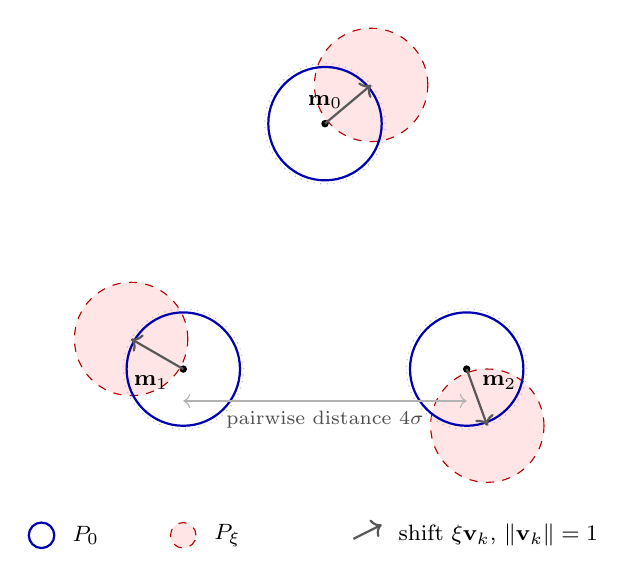
\begin{tikzpicture}[font=\sffamily, scale=0.9]

    % K=3 vertices of a regular simplex in R^{K-1} = R^2: an
    % equilateral triangle with K-independent pairwise distance.
    % Pairwise = 2*sqrt(2)*sigma ~= 2.828, so circumradius =
    % pairwise / sqrt(3) ~= 1.633 for K=3 (or use direct formula
    % R(K=3) = sqrt(2*(K-1)/K)*sigma * sqrt(2*K/(K-1))... wait the
    % cleanest is just use the chord formula).
    \def\rad{2.309}
    \def\rng{0.8}
    \def\shf{0.85}

    \pgfmathsetmacro{\axc}{\rad*cos(90)}
    \pgfmathsetmacro{\ayc}{\rad*sin(90)}
    \pgfmathsetmacro{\bxc}{\rad*cos(210)}
    \pgfmathsetmacro{\byc}{\rad*sin(210)}
    \pgfmathsetmacro{\cxc}{\rad*cos(330)}
    \pgfmathsetmacro{\cyc}{\rad*sin(330)}

    \pgfmathsetmacro{\axQ}{\axc + \shf*cos(40)}
    \pgfmathsetmacro{\ayQ}{\ayc + \shf*sin(40)}
    \pgfmathsetmacro{\bxQ}{\bxc + \shf*cos(150)}
    \pgfmathsetmacro{\byQ}{\byc + \shf*sin(150)}
    \pgfmathsetmacro{\cxQ}{\cxc + \shf*cos(290)}
    \pgfmathsetmacro{\cyQ}{\cyc + \shf*sin(290)}

    \fill[red!10] (\axQ,\ayQ) circle (\rng);
    \draw[red!70!black, dashed, thin] (\axQ,\ayQ) circle (\rng);
    \fill[red!10] (\bxQ,\byQ) circle (\rng);
    \draw[red!70!black, dashed, thin] (\bxQ,\byQ) circle (\rng);
    \fill[red!10] (\cxQ,\cyQ) circle (\rng);
    \draw[red!70!black, dashed, thin] (\cxQ,\cyQ) circle (\rng);

    \draw[gray!50, dotted, thin] (\axc,\ayc) circle (\shf);
    \draw[gray!50, dotted, thin] (\bxc,\byc) circle (\shf);
    \draw[gray!50, dotted, thin] (\cxc,\cyc) circle (\shf);

    \draw[blue!70!black, thick] (\axc,\ayc) circle (\rng);
    \draw[blue!70!black, thick] (\bxc,\byc) circle (\rng);
    \draw[blue!70!black, thick] (\cxc,\cyc) circle (\rng);
    \fill[black] (\axc,\ayc) circle (1.5pt);
    \fill[black] (\bxc,\byc) circle (1.5pt);
    \fill[black] (\cxc,\cyc) circle (1.5pt);

    \draw[->, gray!70!black, thick] (\axc,\ayc) -- (\axQ,\ayQ);
    \draw[->, gray!70!black, thick] (\bxc,\byc) -- (\bxQ,\byQ);
    \draw[->, gray!70!black, thick] (\cxc,\cyc) -- (\cxQ,\cyQ);

    \node[font=\footnotesize, above=2pt] at (\axc,\ayc) {$\mathbf{m}_0$};
    \node[font=\footnotesize, below left=-1pt and 2pt] at (\bxc,\byc) {$\mathbf{m}_1$};
    \node[font=\footnotesize, below right=-1pt and 2pt] at (\cxc,\cyc) {$\mathbf{m}_2$};

    % Pairwise-distance indicator below the bottom edge.
    \pgfmathsetmacro{\midx}{0.5*(\bxc + \cxc)}
    \pgfmathsetmacro{\midy}{\byc - 0.45}
    \draw[gray!60, <->, thin] (\bxc, \midy) -- (\cxc, \midy);
    \node[font=\scriptsize, color=gray!60!black, below] at (\midx, \midy)
        {pairwise distance $4\sigma$};

    \begin{scope}[shift={(-4.0, -3.5)}, font=\footnotesize]
        \draw[blue!70!black, thick] (0,0) circle (0.18);
        \node[anchor=west] at (0.3, 0) {$\mathbb{P}_0$};
        \fill[red!10] (2.0, 0) circle (0.18);
        \draw[red!70!black, dashed, thin] (2.0, 0) circle (0.18);
        \node[anchor=west] at (2.3, 0) {$\mathbb{P}_\xi$};
        \draw[->, gray!70!black, thick] (4.4, -0.05) -- (4.8, 0.15);
        \node[anchor=west] at (4.9, 0) {shift $\xi\mathbf{v}_k$, $\|\mathbf{v}_k\|=1$};
    \end{scope}

\end{tikzpicture}
\end{document}

    \caption{Random per-class mean-shift construction at $K = 3$, the only case that embeds in $\mathbb{R}^2$ (since $K-1 = 2$). The three $\mathbb{P}_0$ class means $\mathbf{m}_k$ (black dots, solid blue rings) sit at the vertices of an equilateral triangle with pairwise distance $4\sigma$ (matching the $K=2$ baseline of the variance experiment). Dotted grey circles show the unit sphere $S^{K-2}$ of allowed shift directions; one realization of the random shifts $\mathbf{v}_k$ is shown as grey arrows of length $\xi$ from each $\mathbf{m}_k$ to the corresponding $\mathbb{P}_\xi$ centroid (dashed red ring). The directions of the three shifts are drawn independently, so the induced perturbation of $\boldsymbol{\eta}(x)$ at every sample point spreads over multiple simplex coordinates rather than concentrating on a single class boundary.}%
    \label{fig:misspec-sensitivity-meanshift-setup}
\end{figure}

Under this construction the per-class Euclidean shift magnitude $\xi$ is K-independent by design. The induced per-class KL divergence between $\mathbb{P}_0$ and $\mathbb{P}_\xi$ reduces to $\xi^2/(2\sigma^2)$, again independent of $K$ (Appendix~\ref{app:kl_invariance}). The horizontal axis is therefore deterministic in $\xi$ even though the per-class shift directions are random per seed. The pairwise inter-class distance is fixed by the choice of $R_{\mathrm{circ}}(K)$. The number of classes, and with it the ambient dimension $K-1$, still varies with $K$.

The cost matrix is again the Asymmetric $10\times$ family, and we also report the Symmetric $0/1$ loss as the cost configuration the variance experiment cannot probe. By analogy with the variance setup, we report the relative excess risk $(R_\xi(h^*_0) - R_\xi(h^*_\xi))/R_\xi(h^*_\xi)$, where $R_\xi(h) = \mathbb{E}_{\mathbb{P}_\xi}[C_{Y, h(X)}]$ is the expected risk under $\mathbb{P}_\xi$, the misspecified classifier $h^*_0(x) = \delta^*(\boldsymbol{\eta}_0(x))$ is built from the unperturbed conditional class probabilities, and the oracle $h^*_\xi(x) = \delta^*(\boldsymbol{\eta}_\xi(x))$ from the perturbed ones.

\begin{figure}[H]
    \centering
    % Auto-generated by experiments.analysis.generate_meanshift_figure --- do not edit.
% K mutually equidistant centroids in R^{K-1}; per-class iid unit shifts of magnitude xi (sigma = 1). Horizontal axis is
% xi/sigma, the per-class Euclidean shift magnitude in units of class
% noise. Top row log-log, bottom row linear; bands are normal-approx
% 95% CIs from mean +/- 1.96 * SE across seeds.
\noindent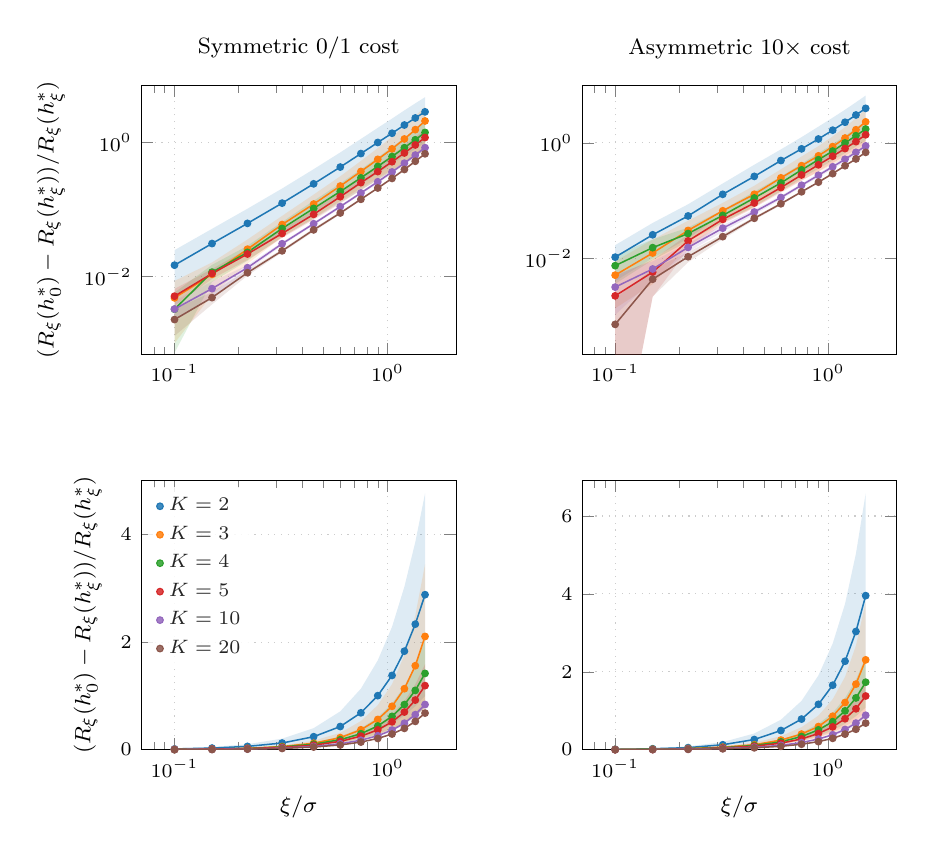
\begin{tikzpicture}
\begin{groupplot}[
    group style={group size=2 by 2, horizontal sep=1.6cm, vertical sep=1.6cm},
    width=0.46\textwidth, height=5.0cm,
    grid=major, grid style={dotted, gray!40},
    xmode=log,
    tick label style={font=\scriptsize},
    label style={font=\footnotesize},
    title style={font=\footnotesize},
]
\nextgroupplot[
    title={Symmetric $0/1$ cost},
    ylabel={$(R_\xi(h^{\ast}_0) - R_\xi(h^{\ast}_\xi)) / R_\xi(h^{\ast}_\xi)$},
    ymode=log,
    xmin=0.07, xmax=2.1, ymin=0.000685695, ymax=7.15445,
]
\addplot[name path=lo_sym_log_K2, draw=none, forget plot] coordinates {
        (0.1, 0.00479413)
        (0.15, 0.0106267)
        (0.22, 0.0214577)
        (0.32, 0.0432953)
        (0.45, 0.0839113)
        (0.6, 0.149655)
        (0.75, 0.238141)
        (0.9, 0.348816)
        (1.05, 0.47909)
        (1.2, 0.635607)
        (1.35, 0.809838)
        (1.5, 0.999864)
    };
\addplot[name path=hi_sym_log_K2, draw=none, forget plot] coordinates {
        (0.1, 0.0248536)
        (0.15, 0.0517165)
        (0.22, 0.10322)
        (0.32, 0.206799)
        (0.45, 0.401742)
        (0.6, 0.714299)
        (0.75, 1.13604)
        (0.9, 1.66378)
        (1.05, 2.28639)
        (1.2, 3.03259)
        (1.35, 3.86369)
        (1.5, 4.76964)
    };
\addplot[color={rgb,255:red,31; green,119; blue,180}, opacity=0.15, forget plot] fill between [of=lo_sym_log_K2 and hi_sym_log_K2];
\addplot[only marks, mark=*, mark size=1.2pt, color={rgb,255:red,31; green,119; blue,180}] coordinates {
        (0.1, 0.0148239)
        (0.15, 0.0311716)
        (0.22, 0.062339)
        (0.32, 0.125047)
        (0.45, 0.242826)
        (0.6, 0.431977)
        (0.75, 0.68709)
        (0.9, 1.0063)
        (1.05, 1.38274)
        (1.2, 1.8341)
        (1.35, 2.33676)
        (1.5, 2.88475)
    };
\addplot[color={rgb,255:red,31; green,119; blue,180}, line width=0.55pt, forget plot] coordinates {
        (0.1, 0.0148239)
        (0.15, 0.0311716)
        (0.22, 0.062339)
        (0.32, 0.125047)
        (0.45, 0.242826)
        (0.6, 0.431977)
        (0.75, 0.68709)
        (0.9, 1.0063)
        (1.05, 1.38274)
        (1.2, 1.8341)
        (1.35, 2.33676)
        (1.5, 2.88475)
    };
\addplot[name path=lo_sym_log_K3, draw=none, forget plot] coordinates {
        (0.1, 0.00101292)
        (0.15, 0.00538669)
        (0.22, 0.0155358)
        (0.32, 0.0390362)
        (0.45, 0.0742413)
        (0.6, 0.135207)
        (0.75, 0.209557)
        (0.9, 0.296696)
        (1.05, 0.394729)
        (1.2, 0.509497)
        (1.35, 0.631362)
        (1.5, 0.762559)
    };
\addplot[name path=hi_sym_log_K3, draw=none, forget plot] coordinates {
        (0.1, 0.00861534)
        (0.15, 0.0162603)
        (0.22, 0.0358173)
        (0.32, 0.0807344)
        (0.45, 0.167964)
        (0.6, 0.314797)
        (0.75, 0.533391)
        (0.9, 0.830348)
        (1.05, 1.2211)
        (1.2, 1.76115)
        (1.35, 2.49511)
        (1.5, 3.45303)
    };
\addplot[color={rgb,255:red,255; green,127; blue,14}, opacity=0.15, forget plot] fill between [of=lo_sym_log_K3 and hi_sym_log_K3];
\addplot[only marks, mark=*, mark size=1.2pt, color={rgb,255:red,255; green,127; blue,14}] coordinates {
        (0.1, 0.00481413)
        (0.15, 0.0108235)
        (0.22, 0.0256765)
        (0.32, 0.0598853)
        (0.45, 0.121102)
        (0.6, 0.225002)
        (0.75, 0.371474)
        (0.9, 0.563522)
        (1.05, 0.807915)
        (1.2, 1.13532)
        (1.35, 1.56324)
        (1.5, 2.10779)
    };
\addplot[color={rgb,255:red,255; green,127; blue,14}, line width=0.55pt, forget plot] coordinates {
        (0.1, 0.00481413)
        (0.15, 0.0108235)
        (0.22, 0.0256765)
        (0.32, 0.0598853)
        (0.45, 0.121102)
        (0.6, 0.225002)
        (0.75, 0.371474)
        (0.9, 0.563522)
        (1.05, 0.807915)
        (1.2, 1.13532)
        (1.35, 1.56324)
        (1.5, 2.10779)
    };
\addplot[name path=lo_sym_log_K4, draw=none, forget plot] coordinates {
        (0.1, 0.00072934)
        (0.15, 0.0083266)
        (0.22, 0.0172268)
        (0.32, 0.0391476)
        (0.45, 0.073082)
        (0.6, 0.127957)
        (0.75, 0.19645)
        (0.9, 0.280219)
        (1.05, 0.381776)
        (1.2, 0.499274)
        (1.35, 0.632871)
        (1.5, 0.781204)
    };
\addplot[name path=hi_sym_log_K4, draw=none, forget plot] coordinates {
        (0.1, 0.00579146)
        (0.15, 0.0149971)
        (0.22, 0.028811)
        (0.32, 0.065496)
        (0.45, 0.135616)
        (0.6, 0.245802)
        (0.75, 0.400127)
        (0.9, 0.603321)
        (1.05, 0.859459)
        (1.2, 1.18244)
        (1.35, 1.57532)
        (1.5, 2.05876)
    };
\addplot[color={rgb,255:red,44; green,160; blue,44}, opacity=0.15, forget plot] fill between [of=lo_sym_log_K4 and hi_sym_log_K4];
\addplot[only marks, mark=*, mark size=1.2pt, color={rgb,255:red,44; green,160; blue,44}] coordinates {
        (0.1, 0.0032604)
        (0.15, 0.0116619)
        (0.22, 0.0230189)
        (0.32, 0.0523218)
        (0.45, 0.104349)
        (0.6, 0.186879)
        (0.75, 0.298288)
        (0.9, 0.44177)
        (1.05, 0.620618)
        (1.2, 0.840859)
        (1.35, 1.1041)
        (1.5, 1.41998)
    };
\addplot[color={rgb,255:red,44; green,160; blue,44}, line width=0.55pt, forget plot] coordinates {
        (0.1, 0.0032604)
        (0.15, 0.0116619)
        (0.22, 0.0230189)
        (0.32, 0.0523218)
        (0.45, 0.104349)
        (0.6, 0.186879)
        (0.75, 0.298288)
        (0.9, 0.44177)
        (1.05, 0.620618)
        (1.2, 0.840859)
        (1.35, 1.1041)
        (1.5, 1.41998)
    };
\addplot[name path=lo_sym_log_K5, draw=none, forget plot] coordinates {
        (0.1, 0.00366337)
        (0.15, 0.00923033)
        (0.22, 0.0177409)
        (0.32, 0.0378419)
        (0.45, 0.0703574)
        (0.6, 0.123427)
        (0.75, 0.195658)
        (0.9, 0.278567)
        (1.05, 0.380557)
        (1.2, 0.498134)
        (1.35, 0.632073)
        (1.5, 0.792972)
    };
\addplot[name path=hi_sym_log_K5, draw=none, forget plot] coordinates {
        (0.1, 0.00654942)
        (0.15, 0.0130258)
        (0.22, 0.0257625)
        (0.32, 0.0502497)
        (0.45, 0.0997646)
        (0.6, 0.188727)
        (0.75, 0.310173)
        (0.9, 0.461311)
        (1.05, 0.657862)
        (1.2, 0.904491)
        (1.35, 1.21642)
        (1.5, 1.59235)
    };
\addplot[color={rgb,255:red,214; green,39; blue,40}, opacity=0.15, forget plot] fill between [of=lo_sym_log_K5 and hi_sym_log_K5];
\addplot[only marks, mark=*, mark size=1.2pt, color={rgb,255:red,214; green,39; blue,40}] coordinates {
        (0.1, 0.00510639)
        (0.15, 0.011128)
        (0.22, 0.0217517)
        (0.32, 0.0440458)
        (0.45, 0.085061)
        (0.6, 0.156077)
        (0.75, 0.252916)
        (0.9, 0.369939)
        (1.05, 0.51921)
        (1.2, 0.701312)
        (1.35, 0.924247)
        (1.5, 1.19266)
    };
\addplot[color={rgb,255:red,214; green,39; blue,40}, line width=0.55pt, forget plot] coordinates {
        (0.1, 0.00510639)
        (0.15, 0.011128)
        (0.22, 0.0217517)
        (0.32, 0.0440458)
        (0.45, 0.085061)
        (0.6, 0.156077)
        (0.75, 0.252916)
        (0.9, 0.369939)
        (1.05, 0.51921)
        (1.2, 0.701312)
        (1.35, 0.924247)
        (1.5, 1.19266)
    };
\addplot[name path=lo_sym_log_K10, draw=none, forget plot] coordinates {
        (0.1, 0.00219756)
        (0.15, 0.00478832)
        (0.22, 0.0122953)
        (0.32, 0.0292442)
        (0.45, 0.0583731)
        (0.6, 0.105202)
        (0.75, 0.168833)
        (0.9, 0.24628)
        (1.05, 0.344181)
        (1.2, 0.46354)
        (1.35, 0.6102)
        (1.5, 0.782947)
    };
\addplot[name path=hi_sym_log_K10, draw=none, forget plot] coordinates {
        (0.1, 0.00436093)
        (0.15, 0.00845224)
        (0.22, 0.0148511)
        (0.32, 0.032712)
        (0.45, 0.0647861)
        (0.6, 0.116745)
        (0.75, 0.18578)
        (0.9, 0.275163)
        (1.05, 0.386317)
        (1.2, 0.524443)
        (1.35, 0.695829)
        (1.5, 0.899684)
    };
\addplot[color={rgb,255:red,148; green,103; blue,189}, opacity=0.15, forget plot] fill between [of=lo_sym_log_K10 and hi_sym_log_K10];
\addplot[only marks, mark=*, mark size=1.2pt, color={rgb,255:red,148; green,103; blue,189}] coordinates {
        (0.1, 0.00327924)
        (0.15, 0.00662028)
        (0.22, 0.0135732)
        (0.32, 0.0309781)
        (0.45, 0.0615796)
        (0.6, 0.110973)
        (0.75, 0.177307)
        (0.9, 0.260721)
        (1.05, 0.365249)
        (1.2, 0.493991)
        (1.35, 0.653014)
        (1.5, 0.841316)
    };
\addplot[color={rgb,255:red,148; green,103; blue,189}, line width=0.55pt, forget plot] coordinates {
        (0.1, 0.00327924)
        (0.15, 0.00662028)
        (0.22, 0.0135732)
        (0.32, 0.0309781)
        (0.45, 0.0615796)
        (0.6, 0.110973)
        (0.75, 0.177307)
        (0.9, 0.260721)
        (1.05, 0.365249)
        (1.2, 0.493991)
        (1.35, 0.653014)
        (1.5, 0.841316)
    };
\addplot[name path=lo_sym_log_K20, draw=none, forget plot] coordinates {
        (0.1, 0.00130057)
        (0.15, 0.00384653)
        (0.22, 0.0103883)
        (0.32, 0.0228958)
        (0.45, 0.0469817)
        (0.6, 0.0849483)
        (0.75, 0.136973)
        (0.9, 0.20328)
        (1.05, 0.282032)
        (1.2, 0.384263)
        (1.35, 0.50756)
        (1.5, 0.654986)
    };
\addplot[name path=hi_sym_log_K20, draw=none, forget plot] coordinates {
        (0.1, 0.00327074)
        (0.15, 0.00587021)
        (0.22, 0.0124935)
        (0.32, 0.0256339)
        (0.45, 0.0527819)
        (0.6, 0.0932644)
        (0.75, 0.148181)
        (0.9, 0.217217)
        (1.05, 0.302976)
        (1.2, 0.410711)
        (1.35, 0.547136)
        (1.5, 0.708301)
    };
\addplot[color={rgb,255:red,140; green,86; blue,75}, opacity=0.15, forget plot] fill between [of=lo_sym_log_K20 and hi_sym_log_K20];
\addplot[only marks, mark=*, mark size=1.2pt, color={rgb,255:red,140; green,86; blue,75}] coordinates {
        (0.1, 0.00228565)
        (0.15, 0.00485837)
        (0.22, 0.0114409)
        (0.32, 0.0242648)
        (0.45, 0.0498818)
        (0.6, 0.0891064)
        (0.75, 0.142577)
        (0.9, 0.210248)
        (1.05, 0.292504)
        (1.2, 0.397487)
        (1.35, 0.527348)
        (1.5, 0.681643)
    };
\addplot[color={rgb,255:red,140; green,86; blue,75}, line width=0.55pt, forget plot] coordinates {
        (0.1, 0.00228565)
        (0.15, 0.00485837)
        (0.22, 0.0114409)
        (0.32, 0.0242648)
        (0.45, 0.0498818)
        (0.6, 0.0891064)
        (0.75, 0.142577)
        (0.9, 0.210248)
        (1.05, 0.292504)
        (1.2, 0.397487)
        (1.35, 0.527348)
        (1.5, 0.681643)
    };
\nextgroupplot[
    title={Asymmetric $10\times$ cost},
    ymode=log,
    xmin=0.07, xmax=2.1, ymin=0.000215628, ymax=9.8693,
]
\addplot[name path=lo_asym_log_K2, draw=none, forget plot] coordinates {
        (0.1, 0.00404221)
        (0.15, 0.0101025)
        (0.22, 0.0220831)
        (0.32, 0.0587623)
        (0.45, 0.107057)
        (0.6, 0.216361)
        (0.75, 0.319181)
        (0.9, 0.424571)
        (1.05, 0.589102)
        (1.2, 0.799497)
        (1.35, 1.03537)
        (1.5, 1.33018)
    };
\addplot[name path=hi_asym_log_K2, draw=none, forget plot] coordinates {
        (0.1, 0.0169239)
        (0.15, 0.0410333)
        (0.22, 0.0863961)
        (0.32, 0.197918)
        (0.45, 0.417872)
        (0.6, 0.770693)
        (0.75, 1.25485)
        (0.9, 1.90792)
        (1.05, 2.72518)
        (1.2, 3.74447)
        (1.35, 5.03355)
        (1.5, 6.57953)
    };
\addplot[color={rgb,255:red,31; green,119; blue,180}, opacity=0.15, forget plot] fill between [of=lo_asym_log_K2 and hi_asym_log_K2];
\addplot[only marks, mark=*, mark size=1.2pt, color={rgb,255:red,31; green,119; blue,180}] coordinates {
        (0.1, 0.010483)
        (0.15, 0.0255679)
        (0.22, 0.0542396)
        (0.32, 0.12834)
        (0.45, 0.262464)
        (0.6, 0.493527)
        (0.75, 0.787016)
        (0.9, 1.16624)
        (1.05, 1.65714)
        (1.2, 2.27198)
        (1.35, 3.03446)
        (1.5, 3.95486)
    };
\addplot[color={rgb,255:red,31; green,119; blue,180}, line width=0.55pt, forget plot] coordinates {
        (0.1, 0.010483)
        (0.15, 0.0255679)
        (0.22, 0.0542396)
        (0.32, 0.12834)
        (0.45, 0.262464)
        (0.6, 0.493527)
        (0.75, 0.787016)
        (0.9, 1.16624)
        (1.05, 1.65714)
        (1.2, 2.27198)
        (1.35, 3.03446)
        (1.5, 3.95486)
    };
\addplot[name path=lo_asym_log_K3, draw=none, forget plot] coordinates {
        (0.1, 0.00136093)
        (0.15, 0.00358624)
        (0.22, 0.016007)
        (0.32, 0.0417922)
        (0.45, 0.0766133)
        (0.6, 0.146798)
        (0.75, 0.224957)
        (0.9, 0.312806)
        (1.05, 0.424596)
        (1.2, 0.552503)
        (1.35, 0.694238)
        (1.5, 0.826407)
    };
\addplot[name path=hi_asym_log_K3, draw=none, forget plot] coordinates {
        (0.1, 0.00887904)
        (0.15, 0.0211426)
        (0.22, 0.0448668)
        (0.32, 0.0913721)
        (0.45, 0.180868)
        (0.6, 0.348829)
        (0.75, 0.579568)
        (0.9, 0.877415)
        (1.05, 1.29664)
        (1.2, 1.86933)
        (1.35, 2.6734)
        (1.5, 3.78737)
    };
\addplot[color={rgb,255:red,255; green,127; blue,14}, opacity=0.15, forget plot] fill between [of=lo_asym_log_K3 and hi_asym_log_K3];
\addplot[only marks, mark=*, mark size=1.2pt, color={rgb,255:red,255; green,127; blue,14}] coordinates {
        (0.1, 0.00511998)
        (0.15, 0.0123644)
        (0.22, 0.0304369)
        (0.32, 0.0665821)
        (0.45, 0.128741)
        (0.6, 0.247813)
        (0.75, 0.402262)
        (0.9, 0.59511)
        (1.05, 0.860619)
        (1.2, 1.21092)
        (1.35, 1.68382)
        (1.5, 2.30689)
    };
\addplot[color={rgb,255:red,255; green,127; blue,14}, line width=0.55pt, forget plot] coordinates {
        (0.1, 0.00511998)
        (0.15, 0.0123644)
        (0.22, 0.0304369)
        (0.32, 0.0665821)
        (0.45, 0.128741)
        (0.6, 0.247813)
        (0.75, 0.402262)
        (0.9, 0.59511)
        (1.05, 0.860619)
        (1.2, 1.21092)
        (1.35, 1.68382)
        (1.5, 2.30689)
    };
\addplot[name path=lo_asym_log_K4, draw=none, forget plot] coordinates {
        (0.1, 0.00360833)
        (0.15, 0.00937548)
        (0.22, 0.0195996)
        (0.32, 0.0417038)
        (0.45, 0.0792056)
        (0.6, 0.143576)
        (0.75, 0.243691)
        (0.9, 0.356287)
        (1.05, 0.494392)
        (1.2, 0.667025)
        (1.35, 0.861869)
        (1.5, 1.08397)
    };
\addplot[name path=hi_asym_log_K4, draw=none, forget plot] coordinates {
        (0.1, 0.0113252)
        (0.15, 0.0212602)
        (0.22, 0.0341269)
        (0.32, 0.0691245)
        (0.45, 0.142751)
        (0.6, 0.261314)
        (0.75, 0.436963)
        (0.9, 0.664554)
        (1.05, 0.94753)
        (1.2, 1.32899)
        (1.35, 1.79871)
        (1.5, 2.38291)
    };
\addplot[color={rgb,255:red,44; green,160; blue,44}, opacity=0.15, forget plot] fill between [of=lo_asym_log_K4 and hi_asym_log_K4];
\addplot[only marks, mark=*, mark size=1.2pt, color={rgb,255:red,44; green,160; blue,44}] coordinates {
        (0.1, 0.00746674)
        (0.15, 0.0153178)
        (0.22, 0.0268632)
        (0.32, 0.0554142)
        (0.45, 0.110979)
        (0.6, 0.202445)
        (0.75, 0.340327)
        (0.9, 0.510421)
        (1.05, 0.720961)
        (1.2, 0.998009)
        (1.35, 1.33029)
        (1.5, 1.73344)
    };
\addplot[color={rgb,255:red,44; green,160; blue,44}, line width=0.55pt, forget plot] coordinates {
        (0.1, 0.00746674)
        (0.15, 0.0153178)
        (0.22, 0.0268632)
        (0.32, 0.0554142)
        (0.45, 0.110979)
        (0.6, 0.202445)
        (0.75, 0.340327)
        (0.9, 0.510421)
        (1.05, 0.720961)
        (1.2, 0.998009)
        (1.35, 1.33029)
        (1.5, 1.73344)
    };
\addplot[name path=lo_asym_log_K5, draw=none, forget plot] coordinates {
        (0.1, 1e-06)
        (0.15, 0.00214183)
        (0.22, 0.0143102)
        (0.32, 0.039251)
        (0.45, 0.0752167)
        (0.6, 0.137255)
        (0.75, 0.220699)
        (0.9, 0.321327)
        (1.05, 0.447093)
        (1.2, 0.596443)
        (1.35, 0.762064)
        (1.5, 0.980136)
    };
\addplot[name path=hi_asym_log_K5, draw=none, forget plot] coordinates {
        (0.1, 0.00496161)
        (0.15, 0.0094138)
        (0.22, 0.0258233)
        (0.32, 0.0553959)
        (0.45, 0.106542)
        (0.6, 0.199316)
        (0.75, 0.335072)
        (0.9, 0.511368)
        (1.05, 0.726727)
        (1.2, 0.996146)
        (1.35, 1.33885)
        (1.5, 1.77886)
    };
\addplot[color={rgb,255:red,214; green,39; blue,40}, opacity=0.15, forget plot] fill between [of=lo_asym_log_K5 and hi_asym_log_K5];
\addplot[only marks, mark=*, mark size=1.2pt, color={rgb,255:red,214; green,39; blue,40}] coordinates {
        (0.1, 0.00224054)
        (0.15, 0.00577782)
        (0.22, 0.0200667)
        (0.32, 0.0473235)
        (0.45, 0.0908795)
        (0.6, 0.168285)
        (0.75, 0.277886)
        (0.9, 0.416347)
        (1.05, 0.58691)
        (1.2, 0.796295)
        (1.35, 1.05045)
        (1.5, 1.3795)
    };
\addplot[color={rgb,255:red,214; green,39; blue,40}, line width=0.55pt, forget plot] coordinates {
        (0.1, 0.00224054)
        (0.15, 0.00577782)
        (0.22, 0.0200667)
        (0.32, 0.0473235)
        (0.45, 0.0908795)
        (0.6, 0.168285)
        (0.75, 0.277886)
        (0.9, 0.416347)
        (1.05, 0.58691)
        (1.2, 0.796295)
        (1.35, 1.05045)
        (1.5, 1.3795)
    };
\addplot[name path=lo_asym_log_K10, draw=none, forget plot] coordinates {
        (0.1, 0.00105006)
        (0.15, 0.00422709)
        (0.22, 0.0128087)
        (0.32, 0.0289705)
        (0.45, 0.0571527)
        (0.6, 0.104925)
        (0.75, 0.172229)
        (0.9, 0.252662)
        (1.05, 0.352477)
        (1.2, 0.473448)
        (1.35, 0.619829)
        (1.5, 0.796576)
    };
\addplot[name path=hi_asym_log_K10, draw=none, forget plot] coordinates {
        (0.1, 0.00530229)
        (0.15, 0.00885979)
        (0.22, 0.0181438)
        (0.32, 0.0375764)
        (0.45, 0.0697994)
        (0.6, 0.121587)
        (0.75, 0.196885)
        (0.9, 0.296651)
        (1.05, 0.417331)
        (1.2, 0.566569)
        (1.35, 0.748686)
        (1.5, 0.972695)
    };
\addplot[color={rgb,255:red,148; green,103; blue,189}, opacity=0.15, forget plot] fill between [of=lo_asym_log_K10 and hi_asym_log_K10];
\addplot[only marks, mark=*, mark size=1.2pt, color={rgb,255:red,148; green,103; blue,189}] coordinates {
        (0.1, 0.00317618)
        (0.15, 0.00654344)
        (0.22, 0.0154762)
        (0.32, 0.0332735)
        (0.45, 0.063476)
        (0.6, 0.113256)
        (0.75, 0.184557)
        (0.9, 0.274657)
        (1.05, 0.384904)
        (1.2, 0.520008)
        (1.35, 0.684258)
        (1.5, 0.884635)
    };
\addplot[color={rgb,255:red,148; green,103; blue,189}, line width=0.55pt, forget plot] coordinates {
        (0.1, 0.00317618)
        (0.15, 0.00654344)
        (0.22, 0.0154762)
        (0.32, 0.0332735)
        (0.45, 0.063476)
        (0.6, 0.113256)
        (0.75, 0.184557)
        (0.9, 0.274657)
        (1.05, 0.384904)
        (1.2, 0.520008)
        (1.35, 0.684258)
        (1.5, 0.884635)
    };
\addplot[name path=lo_asym_log_K20, draw=none, forget plot] coordinates {
        (0.1, 1e-06)
        (0.15, 0.00218368)
        (0.22, 0.00855039)
        (0.32, 0.021457)
        (0.45, 0.0461646)
        (0.6, 0.0835023)
        (0.75, 0.136047)
        (0.9, 0.202113)
        (1.05, 0.283951)
        (1.2, 0.388186)
        (1.35, 0.50797)
        (1.5, 0.656882)
    };
\addplot[name path=hi_asym_log_K20, draw=none, forget plot] coordinates {
        (0.1, 0.00202139)
        (0.15, 0.00651597)
        (0.22, 0.0127907)
        (0.32, 0.026049)
        (0.45, 0.0525555)
        (0.6, 0.092684)
        (0.75, 0.147832)
        (0.9, 0.214878)
        (1.05, 0.302193)
        (1.2, 0.414008)
        (1.35, 0.54467)
        (1.5, 0.711647)
    };
\addplot[color={rgb,255:red,140; green,86; blue,75}, opacity=0.15, forget plot] fill between [of=lo_asym_log_K20 and hi_asym_log_K20];
\addplot[only marks, mark=*, mark size=1.2pt, color={rgb,255:red,140; green,86; blue,75}] coordinates {
        (0.1, 0.000718759)
        (0.15, 0.00434983)
        (0.22, 0.0106705)
        (0.32, 0.023753)
        (0.45, 0.0493601)
        (0.6, 0.0880932)
        (0.75, 0.141939)
        (0.9, 0.208496)
        (1.05, 0.293072)
        (1.2, 0.401097)
        (1.35, 0.52632)
        (1.5, 0.684265)
    };
\addplot[color={rgb,255:red,140; green,86; blue,75}, line width=0.55pt, forget plot] coordinates {
        (0.1, 0.000718759)
        (0.15, 0.00434983)
        (0.22, 0.0106705)
        (0.32, 0.023753)
        (0.45, 0.0493601)
        (0.6, 0.0880932)
        (0.75, 0.141939)
        (0.9, 0.208496)
        (1.05, 0.293072)
        (1.2, 0.401097)
        (1.35, 0.52632)
        (1.5, 0.684265)
    };
\nextgroupplot[
    title={},
    xlabel={$\xi/\sigma$},
    ylabel={$(R_\xi(h^{\ast}_0) - R_\xi(h^{\ast}_\xi)) / R_\xi(h^{\ast}_\xi)$},
    ymode=normal,
    legend style={font=\scriptsize, fill opacity=0.85, draw=none, at={(0.02,0.98)}, anchor=north west},
    legend cell align=left,
    xmin=0.07, xmax=2.1, ymin=0, ymax=5.00812,
]
\addplot[name path=lo_sym_lin_K2, draw=none, forget plot] coordinates {
        (0, 0)
        (0.1, 0.00479413)
        (0.15, 0.0106267)
        (0.22, 0.0214577)
        (0.32, 0.0432953)
        (0.45, 0.0839113)
        (0.6, 0.149655)
        (0.75, 0.238141)
        (0.9, 0.348816)
        (1.05, 0.47909)
        (1.2, 0.635607)
        (1.35, 0.809838)
        (1.5, 0.999864)
    };
\addplot[name path=hi_sym_lin_K2, draw=none, forget plot] coordinates {
        (0, 0)
        (0.1, 0.0248536)
        (0.15, 0.0517165)
        (0.22, 0.10322)
        (0.32, 0.206799)
        (0.45, 0.401742)
        (0.6, 0.714299)
        (0.75, 1.13604)
        (0.9, 1.66378)
        (1.05, 2.28639)
        (1.2, 3.03259)
        (1.35, 3.86369)
        (1.5, 4.76964)
    };
\addplot[color={rgb,255:red,31; green,119; blue,180}, opacity=0.15, forget plot] fill between [of=lo_sym_lin_K2 and hi_sym_lin_K2];
\addplot[only marks, mark=*, mark size=1.2pt, color={rgb,255:red,31; green,119; blue,180}] coordinates {
        (0, 0)
        (0.1, 0.0148239)
        (0.15, 0.0311716)
        (0.22, 0.062339)
        (0.32, 0.125047)
        (0.45, 0.242826)
        (0.6, 0.431977)
        (0.75, 0.68709)
        (0.9, 1.0063)
        (1.05, 1.38274)
        (1.2, 1.8341)
        (1.35, 2.33676)
        (1.5, 2.88475)
    };
\addplot[color={rgb,255:red,31; green,119; blue,180}, line width=0.55pt, forget plot] coordinates {
        (0, 0)
        (0.1, 0.0148239)
        (0.15, 0.0311716)
        (0.22, 0.062339)
        (0.32, 0.125047)
        (0.45, 0.242826)
        (0.6, 0.431977)
        (0.75, 0.68709)
        (0.9, 1.0063)
        (1.05, 1.38274)
        (1.2, 1.8341)
        (1.35, 2.33676)
        (1.5, 2.88475)
    };
\addplot[name path=lo_sym_lin_K3, draw=none, forget plot] coordinates {
        (0, 0)
        (0.1, 0.00101292)
        (0.15, 0.00538669)
        (0.22, 0.0155358)
        (0.32, 0.0390362)
        (0.45, 0.0742413)
        (0.6, 0.135207)
        (0.75, 0.209557)
        (0.9, 0.296696)
        (1.05, 0.394729)
        (1.2, 0.509497)
        (1.35, 0.631362)
        (1.5, 0.762559)
    };
\addplot[name path=hi_sym_lin_K3, draw=none, forget plot] coordinates {
        (0, 0)
        (0.1, 0.00861534)
        (0.15, 0.0162603)
        (0.22, 0.0358173)
        (0.32, 0.0807344)
        (0.45, 0.167964)
        (0.6, 0.314797)
        (0.75, 0.533391)
        (0.9, 0.830348)
        (1.05, 1.2211)
        (1.2, 1.76115)
        (1.35, 2.49511)
        (1.5, 3.45303)
    };
\addplot[color={rgb,255:red,255; green,127; blue,14}, opacity=0.15, forget plot] fill between [of=lo_sym_lin_K3 and hi_sym_lin_K3];
\addplot[only marks, mark=*, mark size=1.2pt, color={rgb,255:red,255; green,127; blue,14}] coordinates {
        (0, 0)
        (0.1, 0.00481413)
        (0.15, 0.0108235)
        (0.22, 0.0256765)
        (0.32, 0.0598853)
        (0.45, 0.121102)
        (0.6, 0.225002)
        (0.75, 0.371474)
        (0.9, 0.563522)
        (1.05, 0.807915)
        (1.2, 1.13532)
        (1.35, 1.56324)
        (1.5, 2.10779)
    };
\addplot[color={rgb,255:red,255; green,127; blue,14}, line width=0.55pt, forget plot] coordinates {
        (0, 0)
        (0.1, 0.00481413)
        (0.15, 0.0108235)
        (0.22, 0.0256765)
        (0.32, 0.0598853)
        (0.45, 0.121102)
        (0.6, 0.225002)
        (0.75, 0.371474)
        (0.9, 0.563522)
        (1.05, 0.807915)
        (1.2, 1.13532)
        (1.35, 1.56324)
        (1.5, 2.10779)
    };
\addplot[name path=lo_sym_lin_K4, draw=none, forget plot] coordinates {
        (0, 0)
        (0.1, 0.00072934)
        (0.15, 0.0083266)
        (0.22, 0.0172268)
        (0.32, 0.0391476)
        (0.45, 0.073082)
        (0.6, 0.127957)
        (0.75, 0.19645)
        (0.9, 0.280219)
        (1.05, 0.381776)
        (1.2, 0.499274)
        (1.35, 0.632871)
        (1.5, 0.781204)
    };
\addplot[name path=hi_sym_lin_K4, draw=none, forget plot] coordinates {
        (0, 0)
        (0.1, 0.00579146)
        (0.15, 0.0149971)
        (0.22, 0.028811)
        (0.32, 0.065496)
        (0.45, 0.135616)
        (0.6, 0.245802)
        (0.75, 0.400127)
        (0.9, 0.603321)
        (1.05, 0.859459)
        (1.2, 1.18244)
        (1.35, 1.57532)
        (1.5, 2.05876)
    };
\addplot[color={rgb,255:red,44; green,160; blue,44}, opacity=0.15, forget plot] fill between [of=lo_sym_lin_K4 and hi_sym_lin_K4];
\addplot[only marks, mark=*, mark size=1.2pt, color={rgb,255:red,44; green,160; blue,44}] coordinates {
        (0, 0)
        (0.1, 0.0032604)
        (0.15, 0.0116619)
        (0.22, 0.0230189)
        (0.32, 0.0523218)
        (0.45, 0.104349)
        (0.6, 0.186879)
        (0.75, 0.298288)
        (0.9, 0.44177)
        (1.05, 0.620618)
        (1.2, 0.840859)
        (1.35, 1.1041)
        (1.5, 1.41998)
    };
\addplot[color={rgb,255:red,44; green,160; blue,44}, line width=0.55pt, forget plot] coordinates {
        (0, 0)
        (0.1, 0.0032604)
        (0.15, 0.0116619)
        (0.22, 0.0230189)
        (0.32, 0.0523218)
        (0.45, 0.104349)
        (0.6, 0.186879)
        (0.75, 0.298288)
        (0.9, 0.44177)
        (1.05, 0.620618)
        (1.2, 0.840859)
        (1.35, 1.1041)
        (1.5, 1.41998)
    };
\addplot[name path=lo_sym_lin_K5, draw=none, forget plot] coordinates {
        (0, 0)
        (0.1, 0.00366337)
        (0.15, 0.00923033)
        (0.22, 0.0177409)
        (0.32, 0.0378419)
        (0.45, 0.0703574)
        (0.6, 0.123427)
        (0.75, 0.195658)
        (0.9, 0.278567)
        (1.05, 0.380557)
        (1.2, 0.498134)
        (1.35, 0.632073)
        (1.5, 0.792972)
    };
\addplot[name path=hi_sym_lin_K5, draw=none, forget plot] coordinates {
        (0, 0)
        (0.1, 0.00654942)
        (0.15, 0.0130258)
        (0.22, 0.0257625)
        (0.32, 0.0502497)
        (0.45, 0.0997646)
        (0.6, 0.188727)
        (0.75, 0.310173)
        (0.9, 0.461311)
        (1.05, 0.657862)
        (1.2, 0.904491)
        (1.35, 1.21642)
        (1.5, 1.59235)
    };
\addplot[color={rgb,255:red,214; green,39; blue,40}, opacity=0.15, forget plot] fill between [of=lo_sym_lin_K5 and hi_sym_lin_K5];
\addplot[only marks, mark=*, mark size=1.2pt, color={rgb,255:red,214; green,39; blue,40}] coordinates {
        (0, 0)
        (0.1, 0.00510639)
        (0.15, 0.011128)
        (0.22, 0.0217517)
        (0.32, 0.0440458)
        (0.45, 0.085061)
        (0.6, 0.156077)
        (0.75, 0.252916)
        (0.9, 0.369939)
        (1.05, 0.51921)
        (1.2, 0.701312)
        (1.35, 0.924247)
        (1.5, 1.19266)
    };
\addplot[color={rgb,255:red,214; green,39; blue,40}, line width=0.55pt, forget plot] coordinates {
        (0, 0)
        (0.1, 0.00510639)
        (0.15, 0.011128)
        (0.22, 0.0217517)
        (0.32, 0.0440458)
        (0.45, 0.085061)
        (0.6, 0.156077)
        (0.75, 0.252916)
        (0.9, 0.369939)
        (1.05, 0.51921)
        (1.2, 0.701312)
        (1.35, 0.924247)
        (1.5, 1.19266)
    };
\addplot[name path=lo_sym_lin_K10, draw=none, forget plot] coordinates {
        (0, 0)
        (0.1, 0.00219756)
        (0.15, 0.00478832)
        (0.22, 0.0122953)
        (0.32, 0.0292442)
        (0.45, 0.0583731)
        (0.6, 0.105202)
        (0.75, 0.168833)
        (0.9, 0.24628)
        (1.05, 0.344181)
        (1.2, 0.46354)
        (1.35, 0.6102)
        (1.5, 0.782947)
    };
\addplot[name path=hi_sym_lin_K10, draw=none, forget plot] coordinates {
        (0, 0)
        (0.1, 0.00436093)
        (0.15, 0.00845224)
        (0.22, 0.0148511)
        (0.32, 0.032712)
        (0.45, 0.0647861)
        (0.6, 0.116745)
        (0.75, 0.18578)
        (0.9, 0.275163)
        (1.05, 0.386317)
        (1.2, 0.524443)
        (1.35, 0.695829)
        (1.5, 0.899684)
    };
\addplot[color={rgb,255:red,148; green,103; blue,189}, opacity=0.15, forget plot] fill between [of=lo_sym_lin_K10 and hi_sym_lin_K10];
\addplot[only marks, mark=*, mark size=1.2pt, color={rgb,255:red,148; green,103; blue,189}] coordinates {
        (0, 0)
        (0.1, 0.00327924)
        (0.15, 0.00662028)
        (0.22, 0.0135732)
        (0.32, 0.0309781)
        (0.45, 0.0615796)
        (0.6, 0.110973)
        (0.75, 0.177307)
        (0.9, 0.260721)
        (1.05, 0.365249)
        (1.2, 0.493991)
        (1.35, 0.653014)
        (1.5, 0.841316)
    };
\addplot[color={rgb,255:red,148; green,103; blue,189}, line width=0.55pt, forget plot] coordinates {
        (0, 0)
        (0.1, 0.00327924)
        (0.15, 0.00662028)
        (0.22, 0.0135732)
        (0.32, 0.0309781)
        (0.45, 0.0615796)
        (0.6, 0.110973)
        (0.75, 0.177307)
        (0.9, 0.260721)
        (1.05, 0.365249)
        (1.2, 0.493991)
        (1.35, 0.653014)
        (1.5, 0.841316)
    };
\addplot[name path=lo_sym_lin_K20, draw=none, forget plot] coordinates {
        (0, 0)
        (0.1, 0.00130057)
        (0.15, 0.00384653)
        (0.22, 0.0103883)
        (0.32, 0.0228958)
        (0.45, 0.0469817)
        (0.6, 0.0849483)
        (0.75, 0.136973)
        (0.9, 0.20328)
        (1.05, 0.282032)
        (1.2, 0.384263)
        (1.35, 0.50756)
        (1.5, 0.654986)
    };
\addplot[name path=hi_sym_lin_K20, draw=none, forget plot] coordinates {
        (0, 0)
        (0.1, 0.00327074)
        (0.15, 0.00587021)
        (0.22, 0.0124935)
        (0.32, 0.0256339)
        (0.45, 0.0527819)
        (0.6, 0.0932644)
        (0.75, 0.148181)
        (0.9, 0.217217)
        (1.05, 0.302976)
        (1.2, 0.410711)
        (1.35, 0.547136)
        (1.5, 0.708301)
    };
\addplot[color={rgb,255:red,140; green,86; blue,75}, opacity=0.15, forget plot] fill between [of=lo_sym_lin_K20 and hi_sym_lin_K20];
\addplot[only marks, mark=*, mark size=1.2pt, color={rgb,255:red,140; green,86; blue,75}] coordinates {
        (0, 0)
        (0.1, 0.00228565)
        (0.15, 0.00485837)
        (0.22, 0.0114409)
        (0.32, 0.0242648)
        (0.45, 0.0498818)
        (0.6, 0.0891064)
        (0.75, 0.142577)
        (0.9, 0.210248)
        (1.05, 0.292504)
        (1.2, 0.397487)
        (1.35, 0.527348)
        (1.5, 0.681643)
    };
\addplot[color={rgb,255:red,140; green,86; blue,75}, line width=0.55pt, forget plot] coordinates {
        (0, 0)
        (0.1, 0.00228565)
        (0.15, 0.00485837)
        (0.22, 0.0114409)
        (0.32, 0.0242648)
        (0.45, 0.0498818)
        (0.6, 0.0891064)
        (0.75, 0.142577)
        (0.9, 0.210248)
        (1.05, 0.292504)
        (1.2, 0.397487)
        (1.35, 0.527348)
        (1.5, 0.681643)
    };
\legend{$K=2$, $K=3$, $K=4$, $K=5$, $K=10$, $K=20$}
\nextgroupplot[
    title={},
    xlabel={$\xi/\sigma$},
    ymode=normal,
    xmin=0.07, xmax=2.1, ymin=0, ymax=6.90851,
]
\addplot[name path=lo_asym_lin_K2, draw=none, forget plot] coordinates {
        (0, 0)
        (0.1, 0.00404221)
        (0.15, 0.0101025)
        (0.22, 0.0220831)
        (0.32, 0.0587623)
        (0.45, 0.107057)
        (0.6, 0.216361)
        (0.75, 0.319181)
        (0.9, 0.424571)
        (1.05, 0.589102)
        (1.2, 0.799497)
        (1.35, 1.03537)
        (1.5, 1.33018)
    };
\addplot[name path=hi_asym_lin_K2, draw=none, forget plot] coordinates {
        (0, 0)
        (0.1, 0.0169239)
        (0.15, 0.0410333)
        (0.22, 0.0863961)
        (0.32, 0.197918)
        (0.45, 0.417872)
        (0.6, 0.770693)
        (0.75, 1.25485)
        (0.9, 1.90792)
        (1.05, 2.72518)
        (1.2, 3.74447)
        (1.35, 5.03355)
        (1.5, 6.57953)
    };
\addplot[color={rgb,255:red,31; green,119; blue,180}, opacity=0.15, forget plot] fill between [of=lo_asym_lin_K2 and hi_asym_lin_K2];
\addplot[only marks, mark=*, mark size=1.2pt, color={rgb,255:red,31; green,119; blue,180}] coordinates {
        (0, 0)
        (0.1, 0.010483)
        (0.15, 0.0255679)
        (0.22, 0.0542396)
        (0.32, 0.12834)
        (0.45, 0.262464)
        (0.6, 0.493527)
        (0.75, 0.787016)
        (0.9, 1.16624)
        (1.05, 1.65714)
        (1.2, 2.27198)
        (1.35, 3.03446)
        (1.5, 3.95486)
    };
\addplot[color={rgb,255:red,31; green,119; blue,180}, line width=0.55pt, forget plot] coordinates {
        (0, 0)
        (0.1, 0.010483)
        (0.15, 0.0255679)
        (0.22, 0.0542396)
        (0.32, 0.12834)
        (0.45, 0.262464)
        (0.6, 0.493527)
        (0.75, 0.787016)
        (0.9, 1.16624)
        (1.05, 1.65714)
        (1.2, 2.27198)
        (1.35, 3.03446)
        (1.5, 3.95486)
    };
\addplot[name path=lo_asym_lin_K3, draw=none, forget plot] coordinates {
        (0, 0)
        (0.1, 0.00136093)
        (0.15, 0.00358624)
        (0.22, 0.016007)
        (0.32, 0.0417922)
        (0.45, 0.0766133)
        (0.6, 0.146798)
        (0.75, 0.224957)
        (0.9, 0.312806)
        (1.05, 0.424596)
        (1.2, 0.552503)
        (1.35, 0.694238)
        (1.5, 0.826407)
    };
\addplot[name path=hi_asym_lin_K3, draw=none, forget plot] coordinates {
        (0, 0)
        (0.1, 0.00887904)
        (0.15, 0.0211426)
        (0.22, 0.0448668)
        (0.32, 0.0913721)
        (0.45, 0.180868)
        (0.6, 0.348829)
        (0.75, 0.579568)
        (0.9, 0.877415)
        (1.05, 1.29664)
        (1.2, 1.86933)
        (1.35, 2.6734)
        (1.5, 3.78737)
    };
\addplot[color={rgb,255:red,255; green,127; blue,14}, opacity=0.15, forget plot] fill between [of=lo_asym_lin_K3 and hi_asym_lin_K3];
\addplot[only marks, mark=*, mark size=1.2pt, color={rgb,255:red,255; green,127; blue,14}] coordinates {
        (0, 0)
        (0.1, 0.00511998)
        (0.15, 0.0123644)
        (0.22, 0.0304369)
        (0.32, 0.0665821)
        (0.45, 0.128741)
        (0.6, 0.247813)
        (0.75, 0.402262)
        (0.9, 0.59511)
        (1.05, 0.860619)
        (1.2, 1.21092)
        (1.35, 1.68382)
        (1.5, 2.30689)
    };
\addplot[color={rgb,255:red,255; green,127; blue,14}, line width=0.55pt, forget plot] coordinates {
        (0, 0)
        (0.1, 0.00511998)
        (0.15, 0.0123644)
        (0.22, 0.0304369)
        (0.32, 0.0665821)
        (0.45, 0.128741)
        (0.6, 0.247813)
        (0.75, 0.402262)
        (0.9, 0.59511)
        (1.05, 0.860619)
        (1.2, 1.21092)
        (1.35, 1.68382)
        (1.5, 2.30689)
    };
\addplot[name path=lo_asym_lin_K4, draw=none, forget plot] coordinates {
        (0, 0)
        (0.1, 0.00360833)
        (0.15, 0.00937548)
        (0.22, 0.0195996)
        (0.32, 0.0417038)
        (0.45, 0.0792056)
        (0.6, 0.143576)
        (0.75, 0.243691)
        (0.9, 0.356287)
        (1.05, 0.494392)
        (1.2, 0.667025)
        (1.35, 0.861869)
        (1.5, 1.08397)
    };
\addplot[name path=hi_asym_lin_K4, draw=none, forget plot] coordinates {
        (0, 0)
        (0.1, 0.0113252)
        (0.15, 0.0212602)
        (0.22, 0.0341269)
        (0.32, 0.0691245)
        (0.45, 0.142751)
        (0.6, 0.261314)
        (0.75, 0.436963)
        (0.9, 0.664554)
        (1.05, 0.94753)
        (1.2, 1.32899)
        (1.35, 1.79871)
        (1.5, 2.38291)
    };
\addplot[color={rgb,255:red,44; green,160; blue,44}, opacity=0.15, forget plot] fill between [of=lo_asym_lin_K4 and hi_asym_lin_K4];
\addplot[only marks, mark=*, mark size=1.2pt, color={rgb,255:red,44; green,160; blue,44}] coordinates {
        (0, 0)
        (0.1, 0.00746674)
        (0.15, 0.0153178)
        (0.22, 0.0268632)
        (0.32, 0.0554142)
        (0.45, 0.110979)
        (0.6, 0.202445)
        (0.75, 0.340327)
        (0.9, 0.510421)
        (1.05, 0.720961)
        (1.2, 0.998009)
        (1.35, 1.33029)
        (1.5, 1.73344)
    };
\addplot[color={rgb,255:red,44; green,160; blue,44}, line width=0.55pt, forget plot] coordinates {
        (0, 0)
        (0.1, 0.00746674)
        (0.15, 0.0153178)
        (0.22, 0.0268632)
        (0.32, 0.0554142)
        (0.45, 0.110979)
        (0.6, 0.202445)
        (0.75, 0.340327)
        (0.9, 0.510421)
        (1.05, 0.720961)
        (1.2, 0.998009)
        (1.35, 1.33029)
        (1.5, 1.73344)
    };
\addplot[name path=lo_asym_lin_K5, draw=none, forget plot] coordinates {
        (0, 0)
        (0.1, -0.000480527)
        (0.15, 0.00214183)
        (0.22, 0.0143102)
        (0.32, 0.039251)
        (0.45, 0.0752167)
        (0.6, 0.137255)
        (0.75, 0.220699)
        (0.9, 0.321327)
        (1.05, 0.447093)
        (1.2, 0.596443)
        (1.35, 0.762064)
        (1.5, 0.980136)
    };
\addplot[name path=hi_asym_lin_K5, draw=none, forget plot] coordinates {
        (0, 0)
        (0.1, 0.00496161)
        (0.15, 0.0094138)
        (0.22, 0.0258233)
        (0.32, 0.0553959)
        (0.45, 0.106542)
        (0.6, 0.199316)
        (0.75, 0.335072)
        (0.9, 0.511368)
        (1.05, 0.726727)
        (1.2, 0.996146)
        (1.35, 1.33885)
        (1.5, 1.77886)
    };
\addplot[color={rgb,255:red,214; green,39; blue,40}, opacity=0.15, forget plot] fill between [of=lo_asym_lin_K5 and hi_asym_lin_K5];
\addplot[only marks, mark=*, mark size=1.2pt, color={rgb,255:red,214; green,39; blue,40}] coordinates {
        (0, 0)
        (0.1, 0.00224054)
        (0.15, 0.00577782)
        (0.22, 0.0200667)
        (0.32, 0.0473235)
        (0.45, 0.0908795)
        (0.6, 0.168285)
        (0.75, 0.277886)
        (0.9, 0.416347)
        (1.05, 0.58691)
        (1.2, 0.796295)
        (1.35, 1.05045)
        (1.5, 1.3795)
    };
\addplot[color={rgb,255:red,214; green,39; blue,40}, line width=0.55pt, forget plot] coordinates {
        (0, 0)
        (0.1, 0.00224054)
        (0.15, 0.00577782)
        (0.22, 0.0200667)
        (0.32, 0.0473235)
        (0.45, 0.0908795)
        (0.6, 0.168285)
        (0.75, 0.277886)
        (0.9, 0.416347)
        (1.05, 0.58691)
        (1.2, 0.796295)
        (1.35, 1.05045)
        (1.5, 1.3795)
    };
\addplot[name path=lo_asym_lin_K10, draw=none, forget plot] coordinates {
        (0, 0)
        (0.1, 0.00105006)
        (0.15, 0.00422709)
        (0.22, 0.0128087)
        (0.32, 0.0289705)
        (0.45, 0.0571527)
        (0.6, 0.104925)
        (0.75, 0.172229)
        (0.9, 0.252662)
        (1.05, 0.352477)
        (1.2, 0.473448)
        (1.35, 0.619829)
        (1.5, 0.796576)
    };
\addplot[name path=hi_asym_lin_K10, draw=none, forget plot] coordinates {
        (0, 0)
        (0.1, 0.00530229)
        (0.15, 0.00885979)
        (0.22, 0.0181438)
        (0.32, 0.0375764)
        (0.45, 0.0697994)
        (0.6, 0.121587)
        (0.75, 0.196885)
        (0.9, 0.296651)
        (1.05, 0.417331)
        (1.2, 0.566569)
        (1.35, 0.748686)
        (1.5, 0.972695)
    };
\addplot[color={rgb,255:red,148; green,103; blue,189}, opacity=0.15, forget plot] fill between [of=lo_asym_lin_K10 and hi_asym_lin_K10];
\addplot[only marks, mark=*, mark size=1.2pt, color={rgb,255:red,148; green,103; blue,189}] coordinates {
        (0, 0)
        (0.1, 0.00317618)
        (0.15, 0.00654344)
        (0.22, 0.0154762)
        (0.32, 0.0332735)
        (0.45, 0.063476)
        (0.6, 0.113256)
        (0.75, 0.184557)
        (0.9, 0.274657)
        (1.05, 0.384904)
        (1.2, 0.520008)
        (1.35, 0.684258)
        (1.5, 0.884635)
    };
\addplot[color={rgb,255:red,148; green,103; blue,189}, line width=0.55pt, forget plot] coordinates {
        (0, 0)
        (0.1, 0.00317618)
        (0.15, 0.00654344)
        (0.22, 0.0154762)
        (0.32, 0.0332735)
        (0.45, 0.063476)
        (0.6, 0.113256)
        (0.75, 0.184557)
        (0.9, 0.274657)
        (1.05, 0.384904)
        (1.2, 0.520008)
        (1.35, 0.684258)
        (1.5, 0.884635)
    };
\addplot[name path=lo_asym_lin_K20, draw=none, forget plot] coordinates {
        (0, 0)
        (0.1, -0.000583874)
        (0.15, 0.00218368)
        (0.22, 0.00855039)
        (0.32, 0.021457)
        (0.45, 0.0461646)
        (0.6, 0.0835023)
        (0.75, 0.136047)
        (0.9, 0.202113)
        (1.05, 0.283951)
        (1.2, 0.388186)
        (1.35, 0.50797)
        (1.5, 0.656882)
    };
\addplot[name path=hi_asym_lin_K20, draw=none, forget plot] coordinates {
        (0, 0)
        (0.1, 0.00202139)
        (0.15, 0.00651597)
        (0.22, 0.0127907)
        (0.32, 0.026049)
        (0.45, 0.0525555)
        (0.6, 0.092684)
        (0.75, 0.147832)
        (0.9, 0.214878)
        (1.05, 0.302193)
        (1.2, 0.414008)
        (1.35, 0.54467)
        (1.5, 0.711647)
    };
\addplot[color={rgb,255:red,140; green,86; blue,75}, opacity=0.15, forget plot] fill between [of=lo_asym_lin_K20 and hi_asym_lin_K20];
\addplot[only marks, mark=*, mark size=1.2pt, color={rgb,255:red,140; green,86; blue,75}] coordinates {
        (0, 0)
        (0.1, 0.000718759)
        (0.15, 0.00434983)
        (0.22, 0.0106705)
        (0.32, 0.023753)
        (0.45, 0.0493601)
        (0.6, 0.0880932)
        (0.75, 0.141939)
        (0.9, 0.208496)
        (1.05, 0.293072)
        (1.2, 0.401097)
        (1.35, 0.52632)
        (1.5, 0.684265)
    };
\addplot[color={rgb,255:red,140; green,86; blue,75}, line width=0.55pt, forget plot] coordinates {
        (0, 0)
        (0.1, 0.000718759)
        (0.15, 0.00434983)
        (0.22, 0.0106705)
        (0.32, 0.023753)
        (0.45, 0.0493601)
        (0.6, 0.0880932)
        (0.75, 0.141939)
        (0.9, 0.208496)
        (1.05, 0.293072)
        (1.2, 0.401097)
        (1.35, 0.52632)
        (1.5, 0.684265)
    };
\end{groupplot}
\end{tikzpicture}%

    \caption{Relative excess risk under the random per-class mean-shift perturbation of Equation~\eqref{eq:meanshift}, as a function of the per-class Euclidean shift magnitude $\xi/\sigma$. The class means are at $K$ mutually equidistant points in $\mathbb{R}^{K-1}$ with $K$-dependent circumradius $R_{\mathrm{circ}}(K) = 2\sigma\sqrt{2(K-1)/K}$ chosen so the pairwise inter-class distance is the same for every $K$; each class's mean is shifted by an independent random unit direction scaled to magnitude $\xi$. Left column: Symmetric $0/1$ cost. Right column: Asymmetric $10\times$ cost. Shaded bands are normal-approx $95\%$ CIs ($\mathrm{mean} \pm 1.96 \cdot \mathrm{SE}$ across $10$ replicate seeds).}%
    \label{fig:misspec-sensitivity-meanshift}
\end{figure}

Figure~\ref{fig:misspec-sensitivity-meanshift} shows the relative excess risk under both cost matrices. At every fixed $\xi/\sigma$ above the Monte Carlo floor the $K = 2$ curve sits above $K = 3$, $K = 3$ above $K = 4$, and so on down to $K = 20$, in both panels. The $K=2$-to-$K=20$ spread at the right edge of the linear panels is roughly four- to six-fold.

The K-monotone ordering and the position of $K = 2$ at the top both reproduce under symmetric $0/1$ cost, dispatching the cost-coupling caveat raised at the end of Section~\ref{sec:misspec_sensitivity_variance}: the decrease in relative excess risk does not require the asymmetric cost coupling of the variance construction.

The fixed pairwise inter-class distance removes the shrinking adjacent-mean distance of the variance experiment, but not every source of $K$-dependence in the oracle risk: with more classes at the same pairwise distance, the Bayes risk $R_\xi(h^*_\xi)$ still changes with $K$. Because the reported quantity divides by this oracle risk, the plotted decrease concerns excess risk relative to the oracle risk; it does not by itself establish that the absolute excess risk $R_\xi(h^*_0) - R_\xi(h^*_\xi)$ decreases with $K$.

Both experiments show the relative excess risk of the misspecified Bayes-optimal rule decreasing as $K$ grows, under two perturbation modes (variance scaling, per-class random mean shifts) and two cost configurations (Asymmetric $10\times$, Symmetric $0/1$), consistent with the second reading of the section's opening. Because the oracle risk also changes with $K$, this decrease reflects the oracle risk as well as the perturbation geometry. The next section isolates a dimensional-dilution mechanism under explicit assumptions on perturbations in probability space; shifting or rescaling Gaussian class-conditional densities does not guarantee these assumptions.

\section{Mechanism and numerical verification of dimensional dilution}\label{sec:misspec_sensitivity_mechanism}

The K-monotone ordering observed in Figures~\ref{fig:misspec-sensitivity-variance} and~\ref{fig:misspec-sensitivity-meanshift} motivates a candidate geometric explanation. The simplex $\Delta^{K-1}$ has $K-1$ degrees of freedom, while a scalar functional of a probability vector probes only one. An isotropic perturbation of fixed Euclidean radius $r$ in the $(K-1)$-dimensional tangent space of $\Delta^{K-1}$ projects onto any fixed scalar gradient with expected squared overlap $r^2/(K-1)$, the standard concentration-of-measure behaviour of uniform random vectors on a high-dimensional sphere.

The rest of this section makes the observation precise as a lemma, verifies it numerically in a synthetic setting where the assumptions hold by construction, and discusses why the lemma's quantitative exponent does not transfer to the misspecification experiments at finite perturbation magnitude.

\subsection{Pointwise dilution and its integrated form}\label{sec:misspec_sensitivity_lemma}

Throughout this subsection, $\delta : \Delta^{K-1} \to \mathcal{Y}$ denotes a fixed decision rule. The per-sample expected cost of $\delta$ at a probability vector $\mathbf{p} \in \Delta^{K-1}$ is
\begin{equation}\label{eq:per_sample_cost_functional}
    \phi_\delta(\mathbf{p}) := \mathcal{L}_{\delta(\mathbf{p})}(\mathbf{p}) = \mathbf{c}_{\delta(\mathbf{p})}^\top \mathbf{p},
\end{equation}
the global conditional-risk functional $\mathcal{L}_i$ of Section~\ref{sec:multiclass} evaluated at the action $\delta(\mathbf{p})$ that $\delta$ selects at $\mathbf{p}$ (Eq.~\eqref{eq:bayes_optimal_delta}). The integrated cost-sensitive risk of $\delta$ along a curve $X \mapsto \boldsymbol{\eta}(X)$ is $\mathcal{R}(\delta; \boldsymbol{\eta}) := \mathbb{E}_X[\phi_\delta(\boldsymbol{\eta}(X))]$. The experiments of Sections~\ref{sec:misspec_sensitivity_variance} and~\ref{sec:misspec_sensitivity_meanshift} report the integrated regret $\mathcal{R}(\delta_{\mathrm{ref}}; \boldsymbol{\eta}_\theta) - \mathcal{R}(\delta_\theta; \boldsymbol{\eta}_\theta)$, where $\mathbb{P}_\theta$ is the perturbed member of the misspecification family ($\theta = \lambda$ for variance scaling, $\theta = \xi$ for mean shifts) and $\mathbb{P}_{\mathrm{ref}}$ its reference (identity) member, $\delta_{\mathrm{ref}}$ is the Bayes-optimal rule for the reference class probabilities $\boldsymbol{\eta}_{\mathrm{ref}}$, $\delta_\theta$ is the oracle Bayes-optimal rule for the true class probabilities $\boldsymbol{\eta}_\theta$, and the expectation is taken under $\mathbb{P}_\theta$.

A perturbation $\boldsymbol{\epsilon}$ of a probability vector $\boldsymbol{\eta} \in \Delta^{K-1}$ must keep $\boldsymbol{\eta} + \boldsymbol{\epsilon}$ a probability vector, so its entries sum to zero. The set of admissible perturbations is
\begin{equation}\label{eq:perturbation_space}
    V := \{ \mathbf{v} \in \mathbb{R}^K : \mathbf{1}^\top \mathbf{v} = 0 \},
\end{equation}
a $(K-1)$-dimensional linear subspace of $\mathbb{R}^K$. We equip $V$ with the Euclidean inner product inherited from $\mathbb{R}^K$, and measure the size of a perturbation by its Euclidean radius $r := \|\boldsymbol{\epsilon}\|$.

The two ingredients of the mechanism are a smoothness condition on the scalar functional and a directional condition on the perturbation.

\begin{assumption}[Local smoothness]\label{ass:smoothness}
    The measurable functional $\phi : \Delta^{K-1} \to \mathbb{R}$ is differentiable at an interior point $\mathbf{p} \in \Delta^{K-1}$ with gradient $\mathbf{g} \in V$, and there exist a constant $M > 0$ and a smoothness radius $\rho > 0$ such that $\mathbf{p} + \boldsymbol{\epsilon} \in \Delta^{K-1}$ for every $\boldsymbol{\epsilon} \in V$ with $\|\boldsymbol{\epsilon}\| \leq \rho$, and the second-order remainder satisfies
    \begin{equation}\label{eq:smoothness_bound}
        \bigl|\phi(\mathbf{p} + \boldsymbol{\epsilon}) - \phi(\mathbf{p}) - \mathbf{g}^\top \boldsymbol{\epsilon}\bigr| \leq M\,\|\boldsymbol{\epsilon}\|^2 \quad \text{for all } \boldsymbol{\epsilon} \in V \text{ with } \|\boldsymbol{\epsilon}\| \leq \rho.
    \end{equation}
\end{assumption}

The condition is satisfied by the per-sample expected cost $\phi_\delta$ at any interior $\mathbf{p}$ that does not lie on the decision boundary of $\delta$: small perturbations of $\mathbf{p}$ do not flip the chosen action, and on a neighbourhood of $\mathbf{p}$ the functional $\phi_\delta$ is linear in its argument, $\phi_\delta(\mathbf{q}) = \mathbf{c}_{\delta(\mathbf{p})}^\top \mathbf{q}$. The directional derivative along any $\boldsymbol{\epsilon} \in V$ is therefore $\mathbf{c}_{\delta(\mathbf{p})}^\top \boldsymbol{\epsilon}$, and the lemma's gradient (the unique $\mathbf{g} \in V$ representing this directional derivative) is the centered cost column $\mathbf{c}_{\delta(\mathbf{p})} - \bar{c}_{\delta(\mathbf{p})}\mathbf{1}$ with $\bar{c}_i = K^{-1}\mathbf{1}^\top \mathbf{c}_i$, generally nonzero. The second-order remainder in Eq.~\eqref{eq:smoothness_bound} is identically zero because a linear function has no quadratic term in its Taylor expansion.

\begin{assumption}[Diffuse perturbation direction]\label{ass:diffuse}
    The perturbation $\boldsymbol{\epsilon}$ is a random vector taking values in $V$, with distribution uniform on the Euclidean sphere $\{\mathbf{v} \in V : \|\mathbf{v}\| = r\}$ for some $0 < r \leq \rho$.
\end{assumption}

This is a modelling choice rather than a literal description of the perturbations realised by either experiment. It encodes the idea that the misspecification energy is spread over the available directions rather than concentrated on a single pair of classes; without diffusion, the decision problem reduces to a binary subproblem and the mechanism does not apply.

\begin{lemma}[Dimensional dilution]\label{lem:dimensional_dilution}
    Let $K \geq 2$. Under Assumptions~\ref{ass:smoothness} and~\ref{ass:diffuse},
    \begin{equation}\label{eq:dimensional_dilution}
        \mathbb{E}\bigl[(\phi(\mathbf{p} + \boldsymbol{\epsilon}) - \phi(\mathbf{p}))^2\bigr] = \frac{r^2}{K-1}\,\|\mathbf{g}\|^2 + O(r^3).
    \end{equation}
\end{lemma}

\begin{proof}
    Choose an orthonormal basis $\mathbf{b}_1, \ldots, \mathbf{b}_{K-1}$ of $V$ (distinct from the simplex vertices $\mathbf{e}_k$). The Helmert basis $\mathbf{b}_k = (\underbrace{1, \ldots, 1}_{k}, -k, 0, \ldots, 0)/\sqrt{k(k+1)}$ is one such choice, and the argument does not depend on the particular basis. Write $\boldsymbol{\epsilon} = \sum_{k=1}^{K-1} Z_k \mathbf{b}_k$ for scalar coordinates $Z_k = \boldsymbol{\epsilon}^\top \mathbf{b}_k$. Since the $\mathbf{b}_k$ are orthonormal, $\|\boldsymbol{\epsilon}\|^2 = \sum_k Z_k^2$, which equals $r^2$ deterministically by Assumption~\ref{ass:diffuse}. Uniform distribution of $\boldsymbol{\epsilon}$ on the radius-$r$ sphere in $V$ is equivalent to uniform distribution of $(Z_1, \ldots, Z_{K-1})$ on the radius-$r$ sphere in $\mathbb{R}^{K-1}$.

    The uniform distribution on a sphere is invariant under coordinate permutations and sign flips, so $\mathbb{E}[Z_k Z_l] = 0$ for $k \neq l$ and $\mathbb{E}[Z_k^2]$ does not depend on $k$. Combined with $\sum_k \mathbb{E}[Z_k^2] = r^2$, this gives $\mathbb{E}[Z_k^2] = r^2/(K-1)$ for each $k$.

    Since $\mathbf{g} \in V$, we may write $\mathbf{g} = \sum_k (\mathbf{g}^\top \mathbf{b}_k)\,\mathbf{b}_k$, so $\mathbf{g}^\top \boldsymbol{\epsilon} = \sum_k (\mathbf{g}^\top \mathbf{b}_k)\,Z_k$ and
    \begin{equation*}
        \mathbb{E}\bigl[(\mathbf{g}^\top \boldsymbol{\epsilon})^2\bigr] = \sum_k (\mathbf{g}^\top \mathbf{b}_k)^2 \cdot \mathbb{E}[Z_k^2] = \frac{r^2}{K-1} \sum_k (\mathbf{g}^\top \mathbf{b}_k)^2 = \frac{r^2}{K-1}\,\|\mathbf{g}\|^2.
    \end{equation*}
    By Assumption~\ref{ass:smoothness}, $\phi(\mathbf{p} + \boldsymbol{\epsilon}) - \phi(\mathbf{p}) = \mathbf{g}^\top \boldsymbol{\epsilon} + \mathrm{rem}(\boldsymbol{\epsilon})$ with $|\mathrm{rem}(\boldsymbol{\epsilon})| \leq M\,r^2$. Squaring and taking expectations, the cross term $\mathbb{E}[(\mathbf{g}^\top \boldsymbol{\epsilon})\,\mathrm{rem}(\boldsymbol{\epsilon})]$ is bounded in absolute value by $\|\mathbf{g}\| \cdot r \cdot M\,r^2 = O(r^3)$ (Cauchy-Schwarz) and the squared remainder by $M^2\,r^4 = O(r^4)$, yielding Eq.~\eqref{eq:dimensional_dilution}.
\end{proof}

Lemma~\ref{lem:dimensional_dilution} is pointwise: a single probability vector $\mathbf{p}$, a single rule's gradient $\mathbf{g}$. The experiments report quantities averaged over $X \sim \mathbb{P}_\theta$. The following corollary is the integration of the lemma along the curve $X \mapsto \boldsymbol{\eta}(X)$ for a fixed rule.

\begin{corollary}[Integrated dilution]\label{cor:integrated_dilution}
    Let $K \geq 2$. Fix a measurable rule $\delta$ and a measurable curve $X \mapsto \boldsymbol{\eta}(X)$. Suppose there is one radius $\rho > 0$ such that Assumption~\ref{ass:smoothness} holds with that radius at $\boldsymbol{\eta}(X)$ for almost every $X$, with gradient $\mathbf{g}_\delta(X) \in V$ and remainder constant $M(X)$, both square-integrable in $X$. Suppose further that the perturbation $\boldsymbol{\epsilon}(X) \in V$, conditionally on $X$, is uniform on the radius-$r$ sphere in $V$, with $0 < r \leq \rho$. Then
    \begin{equation}\label{eq:integrated_dilution}
        \mathbb{E}_{X,\boldsymbol{\epsilon}}\!\bigl[(\phi_\delta(\boldsymbol{\eta}(X) + \boldsymbol{\epsilon}(X)) - \phi_\delta(\boldsymbol{\eta}(X)))^2\bigr] = \frac{r^2}{K-1}\,\mathbb{E}_X[\|\mathbf{g}_\delta(X)\|^2] + O(r^3).
    \end{equation}
\end{corollary}

\begin{proof}
    Apply Lemma~\ref{lem:dimensional_dilution} conditionally on $X$, then take the outer expectation. The leading term integrates to $\frac{r^2}{K-1}\,\mathbb{E}_X[\|\mathbf{g}_\delta(X)\|^2]$. The conditional remainder is bounded by an absolute constant times $M(X)\,\|\mathbf{g}_\delta(X)\|\,r^3 + M(X)^2\,r^4$; its expectation is finite by the square-integrability of $M$ and $\mathbf{g}_\delta$ together with Cauchy-Schwarz, so the integrated remainder is $O(r^3)$.
\end{proof}

\subsection{Numerical verification of the dilution lemma}\label{sec:misspec_sensitivity_lemma_verification}

We verify the Lemma's leading-order prediction in its native setting: reference probability vectors drawn from a Dirichlet on the simplex interior, and perturbations sampled uniformly on the radius-$r$ sphere in $V$.

We do not attempt the verification on the variance or mean-shift constructions of Sections~\ref{sec:misspec_sensitivity_variance} and~\ref{sec:misspec_sensitivity_meanshift}. Those constructions induce differences $\boldsymbol{\eta}_\theta(X) - \boldsymbol{\eta}_{\mathrm{ref}}(X)$ whose covariance at fixed $X$ depends on the Gaussian geometry of the classes rather than satisfying Assumption~\ref{ass:diffuse}'s uniform-on-sphere distribution, so the lemma's quantitative exponent does not transfer at finite perturbation magnitude. Their empirical content is the K-monotone ordering of relative excess risk in Figures~\ref{fig:misspec-sensitivity-variance} and~\ref{fig:misspec-sensitivity-meanshift}, with which the dilution mechanism is qualitatively consistent.

For each $K \in \{2, 3, 4, 5, 7, 10, 15, 20\}$, perturbation radius $r$, and cost configuration $\mathbf{C}$ (Symmetric $0/1$, Asymmetric $M\times$ for $M \in \{2, 5, 10\}$), we draw $n_p = 400$ reference probability vectors $\mathbf{p}_i \overset{\mathrm{iid}}{\sim} \mathrm{Dir}(a\mathbf{1})$ with symmetric concentration $a = 2$, take $\delta(\mathbf{p}_i) = \arg\min_{j \in \mathcal{Y}} (\mathbf{p}_i^\top \mathbf{C})_j$ as the cost-sensitive action, and form the centered cost column $\mathbf{g}_i = \mathbf{c}_{\delta(\mathbf{p}_i)} - \bar c_{\delta(\mathbf{p}_i)}\mathbf{1}$. At each $\mathbf{p}_i$ we draw $n_{\epsilon} = 1000$ perturbations $\boldsymbol{\epsilon}_{ij}$ uniformly on the radius-$r$ sphere in $V$ (Assumption~\ref{ass:diffuse}). Figure~\ref{fig:lemma-test-setup} illustrates the construction at $K = 3$, where $V$ is two-dimensional and the radius-$r$ sphere is a circle around $\mathbf{p}$ in the simplex tangent plane.

\begin{figure}[H]
    \centering
    \documentclass[tikz, border=10pt]{standalone}
\usepackage{tikz}
\usepackage{amsmath}
\usetikzlibrary{calc, arrows.meta}

\begin{document}
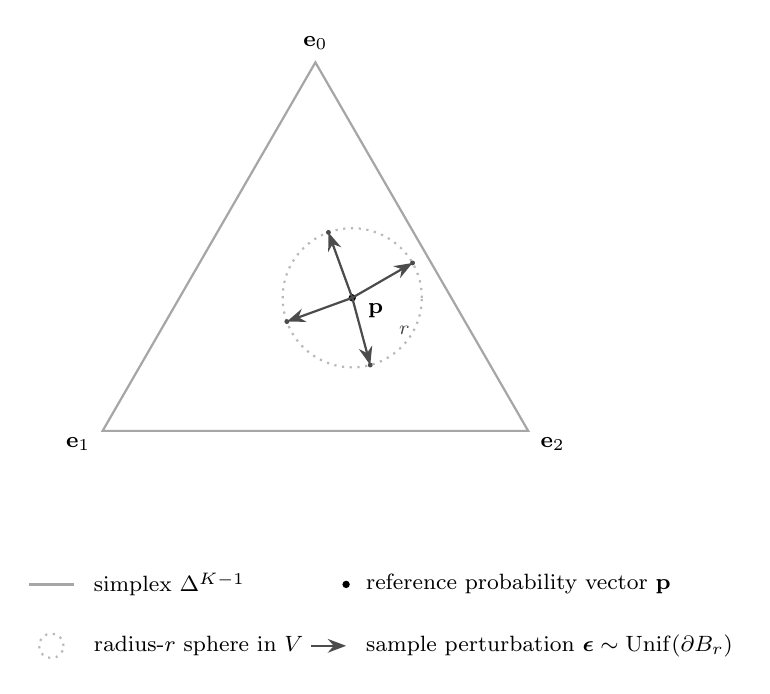
\begin{tikzpicture}[font=\sffamily, scale=2.6]

    % K = 3 case: the simplex Delta^2 embeds in R^3 as the triangle
    % with vertices e_0, e_1, e_2. Drawn here in the 2D centered
    % tangent plane V (a (K-1)-dim subspace of R^K). The radius-r
    % sphere in V is, for K=3, a circle around the reference probability
    % vector p; sample perturbations eps sit on that circle.
    \def\rad{1.2}
    \def\rball{0.34}

    \pgfmathsetmacro{\axc}{\rad*cos(90)}
    \pgfmathsetmacro{\ayc}{\rad*sin(90)}
    \pgfmathsetmacro{\bxc}{\rad*cos(210)}
    \pgfmathsetmacro{\byc}{\rad*sin(210)}
    \pgfmathsetmacro{\cxc}{\rad*cos(330)}
    \pgfmathsetmacro{\cyc}{\rad*sin(330)}

    % Simplex triangle Delta^{K-1}.
    \draw[gray!70, thick]
        (\axc,\ayc) -- (\bxc,\byc) -- (\cxc,\cyc) -- cycle;
    \node[font=\footnotesize, above=1pt] at (\axc,\ayc) {$\mathbf{e}_0$};
    \node[font=\footnotesize, below left=-1pt and 1pt]
        at (\bxc,\byc) {$\mathbf{e}_1$};
    \node[font=\footnotesize, below right=-1pt and 1pt]
        at (\cxc,\cyc) {$\mathbf{e}_2$};

    % Reference probability vector p in the interior, slightly off-center
    % (matching the typical Dirichlet(alpha=2) sample).
    \def\pX{0.18}
    \def\pY{0.05}
    \fill[black] (\pX,\pY) circle (0.018);
    \node[font=\footnotesize, anchor=north west]
        at (\pX+0.03,\pY+0.02) {$\mathbf{p}$};

    % Radius-r sphere in V: at K=3, V is 2-dim and the sphere is a
    % circle around p. Drawn dotted to suggest "set of allowed
    % perturbations".
    \draw[gray!55, dotted, thick] (\pX,\pY) circle (\rball);

    % A handful of sample eps perturbations on the sphere (arrows from p
    % to the circle). Angles chosen to avoid overlap with the labels.
    \foreach \ang in {30, 110, 200, 285} {
        \pgfmathsetmacro{\ux}{\pX + \rball*cos(\ang)}
        \pgfmathsetmacro{\uy}{\pY + \rball*sin(\ang)}
        \draw[->, gray!60!black, thick, >=Stealth]
            (\pX,\pY) -- (\ux,\uy);
        \fill[gray!60!black] (\ux,\uy) circle (0.012);
    }

    % Annotation for the radius.
    \pgfmathsetmacro{\rax}{\pX + \rball*cos(285)*0.55}
    \pgfmathsetmacro{\ray}{\pY + \rball*sin(285)*0.55}
    \node[font=\scriptsize, color=gray!55!black, anchor=west]
        at ($(\pX,\pY)+(0.18,-0.16)$) {$r$};

    % Legend, laid out as a 2x2 grid so it fits under the simplex
    % rather than running past the right edge of the figure.
    \begin{scope}[shift={(-1.40, -1.35)}, font=\footnotesize]
        % Row 1.
        \draw[gray!70, thick] (0, 0) -- (0.22, 0);
        \node[anchor=west] at (0.27, 0)
            {simplex $\Delta^{K-1}$};
        \fill[black] (1.55, 0) circle (0.018);
        \node[anchor=west] at (1.60, 0)
            {reference probability vector $\mathbf{p}$};
        % Row 2.
        \draw[gray!55, dotted, thick] (0.11, -0.30) circle (0.06);
        \node[anchor=west] at (0.27, -0.30)
            {radius-$r$ sphere in $V$};
        \draw[->, gray!60!black, thick, >=Stealth]
            (1.38, -0.30) -- (1.55, -0.30);
        \node[anchor=west] at (1.60, -0.30)
            {sample perturbation $\boldsymbol{\epsilon}\sim\mathrm{Unif}(\partial B_r)$};
    \end{scope}

\end{tikzpicture}
\end{document}

    \caption{Geometry of the synthetic Lemma verification at $K = 3$. The simplex $\Delta^{K-1}$ is the triangle with vertices $\mathbf{e}_0, \mathbf{e}_1, \mathbf{e}_2$. A reference probability vector $\mathbf{p}$ is drawn from $\mathrm{Dir}(a\mathbf{1})$ ($a = 2$) in the interior; perturbations $\boldsymbol{\epsilon}$ are then drawn uniformly on the radius-$r$ sphere of $V$, which at $K = 3$ is the circle of radius $r$ around $\mathbf{p}$ in the simplex tangent plane (dotted). Four sample $\boldsymbol{\epsilon}$ realisations are shown.}%
    \label{fig:lemma-test-setup}
\end{figure}

Lemma~\ref{lem:dimensional_dilution}'s linearised content is the projection identity $\mathbb{E}[(\mathbf{g}^\top \boldsymbol{\epsilon})^2] = r^2/(K-1)\,\|\mathbf{g}\|^2$; integrating over the reference probability vectors,
\begin{equation}\label{eq:lemma_test_prediction}
    \frac{\mathbb{E}_\mathbf{p}\!\left[\mathbb{E}_{\boldsymbol{\epsilon}}\!\bigl[(\mathbf{g}(\mathbf{p})^\top \boldsymbol{\epsilon})^2\bigr]\right]}{\mathbb{E}_\mathbf{p}[\|\mathbf{g}(\mathbf{p})\|^2]} = \frac{r^2}{K-1}.
\end{equation}
This is the Lemma's leading-order claim, exact at any $r$ within the smoothness radius $\rho$ of Assumption~\ref{ass:smoothness}; the higher-order remainder of the lemma's expansion would enter only through nonlinearities of $\phi_\delta$, which are absent for the cost-sensitive functional on the interior of each decision region. Regressing $\log(\mathbb{E}_\mathbf{p}\,\mathbb{E}_{\boldsymbol{\epsilon}}[(\mathbf{g}^\top \boldsymbol{\epsilon})^2] / \mathbb{E}_\mathbf{p}[\|\mathbf{g}\|^2])$ against $\log(K-1)$ at each $r$ recovers the empirical K-decay exponent $\widehat{\gamma}$, which Eq.~\eqref{eq:lemma_test_prediction} predicts to equal $1$ uniformly across cost matrices.

\begin{table}[H]
    \centering
    % Auto-generated by experiments.analysis.generate_lemma_test_table --- do not edit.
\begin{tabular}{lcc}
    \toprule
    Cost configuration & $\widehat{\gamma}$ at $r=0.01$ & $\widehat{\gamma}$ at $r=0.2$ \\
    \midrule
    Symmetric $0/1$ & $1.000$ $[1.000,\,1.000]$ & $1.000$ $[1.000,\,1.000]$ \\
    Asymmetric $2\times$ & $1.000$ $[1.000,\,1.000]$ & $1.000$ $[1.000,\,1.000]$ \\
    Asymmetric $5\times$ & $1.000$ $[0.999,\,1.000]$ & $1.000$ $[0.999,\,1.000]$ \\
    Asymmetric $10\times$ & $1.000$ $[0.999,\,1.000]$ & $1.000$ $[0.999,\,1.000]$ \\
    \bottomrule
\end{tabular}%

    \caption{Fitted K-decay exponent $\widehat{\gamma}$ for the four cost configurations at the smallest and largest swept perturbation radii. At each $r$, $\widehat{\gamma}$ is the negative ordinary-least-squares (OLS) slope of $\log(\mathbb{E}_\mathbf{p}\,\mathbb{E}_{\boldsymbol{\epsilon}}[(\mathbf{g}^\top \boldsymbol{\epsilon})^2] / \mathbb{E}_\mathbf{p}[\|\mathbf{g}\|^2])$ regressed against $\log(K-1)$ across $K \in \{2, 3, 4, 5, 7, 10, 15, 20\}$; bracketed intervals are normal-approx $95\%$ CIs from the OLS slope standard error. Equation~\eqref{eq:lemma_test_prediction} predicts $\widehat{\gamma} = 1$ uniformly across cost matrices and $r$.}%
    \label{tab:lemma-test}
\end{table}

Table~\ref{tab:lemma-test} reports $\widehat{\gamma}$ for the four cost configurations at the smallest swept radius $r = 0.01$ and the largest $r = 0.2$. All entries equal $1$ to three decimal places with sampling-error intervals narrower than $\pm 0.001$. The linearised projection identity holds exactly across cost matrices and radii, as Eq.~\eqref{eq:lemma_test_prediction} predicts.

The non-linear contribution of $\phi_\delta(\mathbf{p} + \boldsymbol{\epsilon}) - \phi_\delta(\mathbf{p})$ on the set where $\boldsymbol{\epsilon}$ flips the cost-sensitive action of $\delta$ is not in the Lemma's regime: Eq.~\ref{eq:smoothness_bound} requires $\|\boldsymbol{\epsilon}\| \leq \rho$, and $\rho$ in turn requires that $\mathbf{p}$ has enough margin from the decision boundaries for the chosen action to be stable in a $\rho$-neighbourhood. This exclusion is why the lemma's exponent transfers cleanly here and not to the variance or mean-shift constructions, whose action-flip events at large perturbations produce the structural deviations from $1/(K-1)$.

\subsection{Scope of the dilution mechanism}\label{sec:misspec_sensitivity_caveats}

The $1/(K-1)$ rate is a property of the linearised functional under an isotropic perturbation of $V$, and neither variance scaling nor mean shifts meet that idealisation. The conditional covariance of $\boldsymbol{\eta}_\theta(X) - \boldsymbol{\eta}_{\mathrm{ref}}(X)$ at fixed $X$ depends on $\boldsymbol{\eta}_{\mathrm{ref}}(X)$ rather than being a scalar multiple of the projector onto $V$, and finite-magnitude perturbations flip decision regions of $\delta$ outside the smoothness regime. The K-monotone ordering observed across both perturbation modes and both cost configurations is consistent with the dilution mechanism, but the exact rate is not expected to transfer.

This suggests a reading of the section's opening observation: the analytical rule may trail the per-row best on a smaller fraction of cost cells in Section~\ref{sec:multiclass_experiments} than in Section~\ref{sec:binary_experiments} because its excess risk relative to the oracle risk decays with $K$, leaving less relative room for a decision-layer correction.

The binary endpoint reads the same way in reverse. At $K = 2$ the relative excess risk climbs steeply with perturbation magnitude in Figures~\ref{fig:misspec-sensitivity-variance} and~\ref{fig:misspec-sensitivity-meanshift}, matching the binary chapter's finding that calibration composed with the analytical rule and direct empirical tuning both improve over the plug-in rule on a substantial fraction of (dataset, model, objective) triples. Empirical tuning continues to help under misspecifications outside the diffuse family considered here (instance-dependent cost shifts, rotational distortions of the kind exploited by Theorem~\ref{thm:rotational_dominance}, or perturbations concentrated on a single pair of classes), while in the two synthetic families the relative excess risk left for it to remove declines with $K$.

Two caveats remain. First, the synthetic comparison is between two known class-probability functions rather than between a fitted estimator and the truth, so the OpenML pattern of Section~\ref{sec:multiclass_experiments} mixes the geometric effect probed here with sample-complexity effects on the tuning side. Second, whether realistic estimator misspecification on a real dataset is diffuse enough for this mechanism to dominate over the worst-case binary-subproblem regime is an open empirical question.

%!TeX root=../carlo_master.tex
\chapter{Conclusion}\label{sec:conclusion}

This dissertation has argued that the decision stage of cost-sensitive classification is a learnable component, separable from the inference estimator that supplies it and small enough to be fit reliably from a held-out partition. The present chapter closes the work in four parts: a chapter-by-chapter summary of the contributions, a practitioner-facing recipe extracted from the campaigns, the scope decisions that bound the claims, and the follow-up directions they invite.

\section{Summary of contributions}

This dissertation treats the decision stage of cost-sensitive classification as a separately optimizable component, distinct from the inference stage that produces the probability estimates it consumes. The motivation is that the analytical plug-in rule incurs excess risk when the probability estimator is miscalibrated under an asymmetric cost structure, the regime that modern classifiers routinely occupy. A held-out optimization of the decision layer corrects decision-level miscalibrations that the analytical rule cannot.

Chapter~\ref{sec:theory} gives the structural reason this correction is admissible: a complexity asymmetry between the two stages. The inference model may be high-complexity and miscalibrated, while the decision class has dimension polynomial in $K$. On a validation sample of size $m$ drawn independently of the estimator fit, the decision layer therefore admits a generalization bound of order $\sqrt{d_\mathrm{dec}/m}$ (Proposition~\ref{prop:gen_bound}).

This capacity argument is necessary, not sufficient. It establishes that the decision layer is learnable in principle, but not that the gain materializes on a given dataset. On a single small held-out split the empirical minimizer can underperform the analytical plug-in. Across both campaigns the improvement is reliable only when the decision layer is selected by cross-validation over the full training pool. The capacity bound makes the procedure statistically sound; it is the cross-validated estimation, not the bound, that produces the improvement in practice.

In the binary setting (Chapters~\ref{sec:binary} and~\ref{sec:binary_experiments}) we derive the analytical Elkan threshold and characterize its fragility under probability miscalibration. The campaign spans fourteen datasets, ten base classifiers, and ten objectives. EmpiricalCV wins or ties the per-row best on $87\%$ of cost cells and $99.9\%$ of maximization-metric cells.

In the multiclass setting (Chapters~\ref{sec:multiclass} through~\ref{sec:multiclass_experiments}) we develop a taxonomy of partition-optimization strategies (the parallel shift and linear class scaling of \citet{obrien2008costsensitive}, the probability-ratio thresholding of \citet{lachiche2003improving} and the multidimensional thresholding of \citet{marchetti2025multidimensional}, each equivalent under $0/1$ loss to one of the O'Brien parameterizations, and a priority-based sequential cascade), grouping the matrix-parameterized classes $\mathcal{H}_{PS} \cup \mathcal{H}_{Sc} \cup \mathcal{H}_{Full}$ under a single framework and identifying $\mathcal{H}_{PS} \cup \mathcal{H}_{Sc}$ as the $K-1$-parameter vector-tuned subset. We compute Natarajan-dimension bounds for the convex-partition score classes: $d_{Nat}(\mathcal{H}_{PS}) = K-1$, $d_{Nat}(\mathcal{H}_{Sc}) \leq K-1$, and $d_{Nat}(\mathcal{H}_{Full}) \leq K^2$. The unconstrained Voronoi class $\mathcal{H}_{Vor}$ of Chapter~\ref{sec:voronoi_tessellation} properly contains $\mathcal{H}_{PS}$ (Proposition~\ref{prop:ps_in_vor}), with strict population risk separation from $\mathcal{H}_{PS}$ exhibited on a $K{=}3$ witness under symmetric $0/1$ loss via the DLC subclass $\mathcal{H}_{Vor}^{\mathrm{DLC}}$ (Theorem~\ref{thm:rotational_dominance}). The class actually fit is $\mathcal{H}_{Vor}^{\mathrm{DLC}} \subseteq \mathcal{H}_{Vor}^{\Delta}$ at $d_{Nat} \leq K^2$, rather than the $d_{Nat} \leq K^2 + K$ unconstrained class on which Proposition~\ref{prop:ps_in_vor} relies.

The cross-validated tuning variants lead the multiclass per-row comparison as in the binary setting. On cost objectives three variants are tied at the top within sampling noise (FullMatrixPartitioningCV at $80\%$, RiskPartitioningCV at $79\%$, LinearScalingCV at $78\%$ win-or-tie); on maximization metrics ThresholdRatioCV leads at $90\%$. The richer Voronoi class does not improve on these: counting cells where a Voronoi variant is the unique SE-overlap winning family, the rate is $0.1\%$ on cost cells and $1.2\%$ on maximization cells. This is consistent with Proposition~\ref{prop:ps_in_vor}, which guarantees only no-worse population risk; the strict advantage of Theorem~\ref{thm:rotational_dominance} requires a rotational regime the OpenML benchmark does not appear to concentrate in.

Chapter~\ref{sec:misspec_sensitivity_K} adds a second-order observation about how the decision-layer advantage depends on $K$. The lead of the best strategy over the bare analytical rule on cost cells narrows from $18$ points in binary ($87\%$ versus $69\%$ win-or-tie) to $11$ points in multiclass ($80\%$ versus $69\%$), so the room for a decision-layer correction narrows as $K$ grows. The dimensional-dilution mechanism predicts this direction qualitatively: a diffuse misspecification of $\boldsymbol{\eta}$ of fixed Euclidean radius projects onto a scalar cost functional with expected squared overlap of order $1/(K-1)$ (Lemma~\ref{lem:dimensional_dilution}), verified to that exponent in a synthetic setting where its assumptions hold by construction. The benchmark comparison and the synthetic mechanism are not equivalent: the benchmark mixes the geometric effect with sample-complexity effects on the tuning side, and the lemma's quantitative exponent does not transfer at finite perturbation magnitude in the variance-scaling and mean-shift experiments.

\section{A practitioner recipe}\label{sec:practitioner_recipe}

The campaigns support a short rule of thumb. Use a cross-validated decision-layer tuner whenever the training data supports it: EmpiricalCV in binary and, in multiclass, FullMatrixPartitioningCV, RiskPartitioningCV, or LinearScalingCV for cost-decomposable objectives, and ThresholdRatioCV for non-decomposable maximization metrics. These strategies lead every campaign aggregate in this dissertation, from $87\%$ and $99.9\%$ for EmpiricalCV on binary cost and maximization cells to the $78$--$80\%$ band on multiclass cost cells and $90\%$ on multiclass maximization cells. The one exception is a well-calibrated estimator (the three deep tabular models in their supported regimes) paired with a cost-decomposable objective, where the bare Analytical plug-in is competitive within sampling noise and consumes no held-out data.

Two operational caveats follow. First, the empirical family beats the analytical plug-in only when the full training pool funds the tuning: single-split Empirical on the $10\%$ validation partition wins or ties just $42\%$ of binary cost cells, below the bare Analytical's $69\%$, so an in-budget held-out split is not a substitute for cross-validating over the full $80\%$ pool. Second, the richer partition classes earn their parameters only when the data supplies a matching signal. VoronoiTuning is appropriate when the estimator's miscalibration rotates the optimal boundaries (the regime constructed in Section~\ref{sec:boundary_rotation_experiment}); the OpenML pool does not concentrate there, and the vector-tuned and full-matrix CV variants meet or beat it within sampling noise on both objective groups.

\section{Limitations}

Nine scope decisions bound the claims above and invite extension.

\begin{enumerate}
    \item The evaluation protocol is fixed throughout the campaigns: $80/20$ train-test, with a $70/10$ train/validation split inside the train-full pool for the single-split tuners and $5$-fold stratified cross-validation over the full $80\%$ pool for the CV variants. How the per-strategy rankings vary with these knobs (a tighter or looser validation partition, a different fold count, or repeated CV) is not investigated.
    \item The per-strategy search ranges (for instance $\boldsymbol{\Delta} \in [-1, 1]^{K \times K}$ for FullMatrixPartitioning, $b_k \in [-1, 1]$ for MultidimensionalThreshold, $\tau_k \in [0.01, 1.5]$ for ThresholdRatio) are fixed by a single up-front choice rather than adapted per dataset, classifier, objective, or cost-matrix scale. A more carefully designed search space (rescaling $\boldsymbol{\Delta}$ by $C_{\max}$ to track the anchor magnitude, widening the parallel-shift band on objectives where the best $\mathbf{b}$ sits near the search boundary, or per-regime tuning) could move any of the tuning variants in either direction, so the per-strategy rankings reflect both the strategies themselves and the specific ranges adopted here.
    \item The Voronoi optimization relies on stochastic local search, since the empirical risk is piecewise constant in the prototype configuration. A differentiable surrogate (for instance, a softmax-temperature relaxation of the nearest-prototype assignment) would admit first-order methods. The sampling distribution that feeds the search is a separate axis: the experiments use the sequential $d^2$ sampler of Section~\ref{sec:voronoi_samplers}, adopted as the only one of the six surveyed there that satisfies~\eqref{eq:dlc} with probability one across the full $K$ sweep, but a sampler biased toward the analytical-parallel-shift seed, or one that relaxes the DLC in exchange for wider coverage of $\mathcal{H}_{Vor}^{\Delta}$, is unexplored. Either change may reduce the gap between the matrix-parameterized methods and Voronoi observed on the OpenML benchmark.
    \item The multiclass benchmark covers $K \leq 10$. Whether the empirical Pareto-dominance of the matrix-parameterized methods over Voronoi inverts at larger $K$, where the additional rotational degrees of freedom grow quadratically in $K$, is left open.
    \item The models are evaluated at default parameters only. A controlled study of how decision-layer tuning interacts with base-estimator calibration quality across model capacities would refine the practical recommendations of Section~\ref{sec:practitioner_recipe}.
    \item The benchmark draws exclusively from tabular OpenML datasets and tabular-oriented base classifiers (logistic regression, gradient-boosted trees, random forests, and three deep tabular architectures). Whether the per-strategy rankings and the recommendations of Section~\ref{sec:practitioner_recipe} transfer to non-tabular multiclass settings (image classification with convolutional or transformer backbones, text classification with language-model embeddings, time-series, audio, or graph classification) is an open question; the calibration profiles and typical cost-asymmetry regimes practitioners face in those domains may differ enough that a separate benchmark is required.
    \item The calibrate-then-decide strategies fit on the $10\%$ validation partition while their direct-tuning CV counterparts use the full $80\%$ pool, a roughly sevenfold gap in label budget. The natural matched-budget protocol is to cross-validate the calibrator parameters as hyperparameters, the same treatment the CV tuning variants give to thresholds and partition parameters; this is left outside scope, and the calibrate-then-decide rankings are read as conditional on the budget asymmetry.
    \item The $1/(K-1)$ dilution exponent is a property of the linearized cost functional under an isotropic perturbation of the simplex tangent space. The variance-scaling and mean-shift experiments reproduce the K-monotone ordering but not the exact exponent at finite perturbation magnitude. Whether realistic estimator misspecification on a real dataset is sufficiently diffuse for this mechanism to dominate over the worst-case binary-subproblem regime is an open question.
    \item Running the campaigns end-to-end is non-trivially expensive (Appendix~\ref{app:compute} documents the wall-clock and cloud-spend footprint, together with the harness optimisations that brought the multiclass campaign down by an order of magnitude). The compute floor constrained how many of the axes flagged in the limitations above could be explored: sweeping the validation-split size, the fold count, or the per-strategy search ranges, or adding seeds, datasets, or estimator-capacity ablations, would have required compute beyond what was budgeted for this work.
\end{enumerate}

\section{Future work}

The two-stage formulation leaves four natural follow-up directions.

\paragraph{Cost-into-loss training.} The alternative paradigm set aside in this dissertation folds the cost structure into the training objective rather than pushing it to the decision stage. Cost-weighted cross-entropy, focal loss, and differentiable surrogates for confusion-matrix metrics, including the Score-Oriented Loss framework of \citet{marchetti2022sol}, are the main candidates. The two routes are not mutually exclusive: a cost-weighted training objective can still be paired with a tuned decision rule. A controlled comparison on the benchmarks of Chapters~\ref{sec:binary_experiments} and~\ref{sec:multiclass_experiments} would quantify when integrating the cost into the loss replaces, complements, or is dominated by tuning at the decision stage.

\paragraph{Richer cost structure.} The cost matrix is treated here as a fixed constant. Many applied settings carry costs that depend on the input (fraud detection where the loss scales with transaction value, medical triage where the misclassification cost depends on patient characteristics), on time (drift, deteriorating signal, deadlines), or on group membership (fairness constraints expressed as group-conditional miscalibration penalties). Extending the partition-optimization framework to $\mathbf{C}(x)$, $\mathbf{C}(t)$, or $\mathbf{C}(g)$ requires reformulating $\mathcal{H}_{PS}$, for instance, as parameter fields over the conditioning variable rather than constants on the simplex; the analytical plug-in rule extends in form, since it is already a pointwise minimization $\arg\min_k \mathbf{c}_k^\top \boldsymbol{\eta}(x)$ at each $x$ and only the cost vector needs to be queried at the conditioning variable, but the empirical-tuning machinery does not transfer immediately, since the partition parameters themselves become $x$-, $t$-, or $g$-indexed.

\paragraph{Argmax as the default elsewhere in ML.} The decision-stage perspective developed here is one specialization of a recurring pattern: in many machine-learning pipelines a selection step (whether final or repeated inside the pipeline) is a learnable design choice that the standard implementation forgoes by defaulting to argmax or its top-$k$ cousin. In autoregressive language-model decoding, greedy next-token selection gives way to temperature sampling, nucleus and top-$k$ sampling \citep{holtzman2020curious}, beam search, and contrastive or speculative decoding. In reinforcement learning and contextual bandits \citep{sutton2018reinforcement}, the entire exploration literature exists to improve on greedy argmax over value estimates ($\varepsilon$-greedy, Boltzmann sampling, UCB, Thompson sampling); modern actor-critic methods (PPO, SAC) replace deterministic argmax policies with stochastic ones, with entropy regularization explicitly penalizing argmax collapse, and risk-sensitive RL replaces expected-return-argmax with CVaR or distortion-based action rules \citep{tamar2015cvar}, a direct analogue of the cost-sensitive theme here. The pattern recurs in semantic segmentation (per-pixel argmax versus learned decoders or CRF post-processing \citep{krahenbuhl2011efficient}), in retrieval and recommendation (top-$k$ cutoffs and ranking-aware thresholds), in selective classification (predict-vs-abstain thresholds, \citealp{geifman2017selective}), and in object detection (the confidence threshold of non-maximum suppression, \citealp{bodla2017soft}). Each of these has a learnable or cost-aware variant that the standard pipeline silently forgoes.

\paragraph{Releasing the library.} The decision strategies of this dissertation are implemented in \texttt{threshold\_opt}, a Python library that follows the scikit-learn \citep{pedregosa2011scikit} estimator conventions: every strategy inherits from a common \texttt{DecisionStrategy} base class and exposes a \texttt{fit(X, y, objective)} / \texttt{predict(X)} pair, with composable post-hoc calibrators, a vectorised cost-aware metric implementation, and the harness optimisations of Appendix~\ref{app:compute} on the experiment side. Finalising the public-API documentation, type annotations, and PyPI release is a concrete follow-up. Decision-stage tuning is a step that practitioners commonly skip, defaulting to the cost-blind argmax; the campaigns in this dissertation suggest that the gap on miscalibrated estimators and non-decomposable objectives is large enough to warrant a library that makes adopting the decision-layer step as routine as fitting a calibrator.

The argmax that ships with every off-the-shelf classifier is a choice, not a constant. When the estimator is well-calibrated and the objective is cost-decomposable, Bayesian decision theory supplies the answer in closed form: the analytical Elkan threshold and its multiclass partition boundary are competitive without any held-out tuning. When the estimator is miscalibrated or the objective is non-decomposable, the answer is a learnable rule, fit on a validation partition with the same care as a calibrator. The decision stage is small enough to learn; the cost of leaving it at the cost-blind default is large enough to matter.


%%%%%%%%%%%%%%%%%%%%%%%%%%%%%%%% APPENDICES %%%%%%%%%%%%%%%%%%%%%%%%%%%%%%%%%%%%

\cleardoublepage

\pagestyle{appendix}

\appendix

\addappheadtotoc

%!TeX root=../carlo_master.tex
\chapter{Supplementary proofs}\label{app:supplementary_proofs}

This appendix collects proofs and verifications deferred from the main text for readability: the Bayes risk identity (Proposition~\ref{prop:bayes_risk_identity}, Chapter~\ref{sec:theory}), the unit VC dimension of one-dimensional threshold functions (Lemma~\ref{lem:vc_thresh}, Chapter~\ref{sec:theory}), the optimality of the calibrate-then-decide pipeline (Proposition~\ref{prop:calibrate_then_decide}, Chapter~\ref{sec:binary}), the admissibility verifications behind Examples~\ref{ex:inadmissible} and~\ref{ex:hedge} together with the proof of Proposition~\ref{prop:elementwise_admissible} (Chapter~\ref{sec:multiclass}), and the vertical-stack witness for the strict risk separation between the Voronoi and parallel-shift classes (Theorem~\ref{thm:rotational_dominance}, Chapter~\ref{sec:voronoi_tessellation}).

\begin{proof}[Proof of Proposition~\ref{prop:bayes_risk_identity}]
Since each map $x \mapsto \mathcal{R}(\hat{y} \mid x)$ is $\Sigma_{\mathcal{X}}$-measurable for every fixed $\hat{y} \in \mathcal{Y}$ and $\mathcal{Y}$ is finite, the level sets
\begin{equation*}
\begin{split}
    \{x \in \mathcal{X} \mid h^*(x) = k\} = {}& \bigcap_{j > k}\{x \in \mathcal{X} \mid \mathcal{R}(k \mid x) \leq \mathcal{R}(j \mid x)\} \\
    & {} \cap \bigcap_{j < k}\{x \in \mathcal{X} \mid \mathcal{R}(k \mid x) < \mathcal{R}(j \mid x)\}
\end{split}
\end{equation*}
are finite Boolean combinations of measurable sets, so $h^*$ is $\Sigma_{\mathcal{X}}/\Sigma_{\mathcal{Y}}$-measurable and $h^* \in \mathcal{H}_{all}$. Boundedness of $\mathbf{C}$ ensures $0 \leq \mathcal{R}(\hat{y} \mid x) \leq C_{max}$ for every $\hat{y}$ and $x$, so $R(h)$ is finite for all $h \in \mathcal{H}_{all}$ and the Lebesgue integral is well-defined.

For every $h \in \mathcal{H}_{all}$ and every $x \in \mathcal{X}$, the pointwise bound $\mathcal{R}(h(x) \mid x) \geq \min_{\hat{y} \in \mathcal{Y}} \mathcal{R}(\hat{y} \mid x)$ holds; monotonicity of the Lebesgue integral lifts this to $R(h) \geq \mathbb{E}_X[\min_{\hat{y}} \mathcal{R}(\hat{y} \mid X)]$. Since $h^*$ attains the pointwise minimum at every $x \in \mathcal{X}$ and lies in $\mathcal{H}_{all}$, this lower bound is realized at $h^*$, which proves Eq.~(\ref{eq:bayes_risk_identity}).
\end{proof}

\begin{proof}[Proof of Lemma~\ref{lem:vc_thresh}]
We show that $\mathcal{H}_{thresh}$ can shatter a set of size 1 but cannot shatter any set of size 2.

First, we establish the lower bound $d_{VC} \geq 1$. Consider a set containing a single probability estimate $z_1 = 0.5$. We can generate all $2^1$ possible labelings by varying $\tau$. If we select a threshold $\tau = 0.6$, the decision rule yields $\delta_{0.6}(0.5) = 0$ since $0.5 < 0.6$. Conversely, if we select $\tau = 0.4$, the rule yields $\delta_{0.4}(0.5) = 1$ since $0.5 \geq 0.4$. As the classifier can assign both possible labels to the point, the set is shattered.

Next, we establish the upper bound $d_{VC} < 2$ by contradiction. Consider an arbitrary set of two distinct points $\{z_1, z_2\} \subset [0, 1]$. Without loss of generality, assume the points are ordered such that $z_1 < z_2$. For the set to be shattered, there must exist thresholds capable of producing all $2^2 = 4$ dichotomies. However, consider the specific labeling assignment $(y_1=1, y_2=0)$. For the hypothesis $\delta_\tau$ to predict $y_1=1$, we require $z_1 \geq \tau$. Simultaneously, to predict $y_2=0$, we require $z_2 < \tau$. These two conditions require that $z_1 \geq \tau > z_2$. Combining $z_1 \geq \tau$ with $\tau > z_2$ yields $z_1 > z_2$ by transitivity, which contradicts our initial assumption that $z_1 < z_2$. Therefore, it is impossible to assign a positive label to the smaller value while assigning a negative label to the larger value. Since at least one labeling is unattainable, no set of size 2 can be shattered.

We conclude that $d_{VC}(\mathcal{H}_{thresh}) = 1$.
\end{proof}

\begin{proof}[Proof of Proposition~\ref{prop:calibrate_then_decide}]
Under the stated condition, $\delta_g(x) = \mathbb{I}(\eta(x) \geq p^*)$. By Lemma~\ref{lem:threshold_optimality}, this attains the minimum conditional risk at every $x$ (it agrees with the smallest-index Bayes rule of Eq.~\eqref{eq:bayes_optimal} off the risk-neutral tie set $\{\eta = p^*\}$, where both actions are risk-minimizers), so $\delta_g$ attains the Bayes risk and coincides with $h^*$ in risk.
\end{proof}

\begin{proof}[Verification of Example~\ref{ex:inadmissible}]
Class~1 is not strictly dominated element-wise by any single alternative class: it is superior to Class~0 when the true class is~2 ($6 < 10$) and superior to Class~2 when the true class is~0, so its inadmissibility is not detectable from the entries of $\mathbf{C}$ alone. The risk of action 1 is nonetheless strictly greater than the minimum risk of the alternative actions at every vertex of the probability simplex. When the class probability is concentrated on Class 0 ($\mathbf{p} = \mathbf{e}_0$), the optimal decision is Class 0 (risk 0). When the class probability is concentrated on Class 2 ($\mathbf{p} = \mathbf{e}_2$), the optimal decision is Class 2 (risk 0). Even when the class probability is concentrated on Class 1 ($\mathbf{p} = \mathbf{e}_1$), predicting Class 1 incurs a cost of 6, whereas predicting either Class 0 or Class 2 incurs a lower cost of 4. Since the conditional risk functions $\mathcal{L}_i(\mathbf{p}) = \mathbf{c}_i^\top \mathbf{p}$ are linear, the constant risk surface of action~1 ($\mathbf{c}_1^\top \mathbf{p} = 6$) lies strictly above the pointwise lower envelope $\min(\mathcal{L}_0, \mathcal{L}_2)$ of the two competing actions, whose maximum over $\Delta^{K-1}$ is $5$, attained at $\mathbf{p} = (\tfrac{1}{2}, 0, \tfrac{1}{2})$. Consequently, there exists no point $\mathbf{p} \in \Delta^{K-1}$ where action 1 minimizes the expected loss, rendering the decision region $\mathcal{P}_1^*$ empty and the matrix inadmissible.
\end{proof}

\begin{proof}[Verification of Example~\ref{ex:hedge}]
Classes~$0$ and~$1$ form a costly confusable pair: predicting one when the other is true incurs a cost of $10$. Class~$2$ is a low-stakes hedge, costing $2$ to predict whether the truth is $0$ or $1$, while a correct prediction of class~$2$ costs~$5$. The matrix is admissible. Predicting class $0$ is the unique risk-minimizer at $\mathbf{e}_0$, with cost $0$ against $10$ and $2$, and predicting class $1$ at $\mathbf{e}_1$ by symmetry. Predicting class $2$ is the unique risk-minimizer at $\mathbf{p} = (\tfrac{1}{2}, \tfrac{1}{2}, 0)$, where its risk $\mathbf{c}_2^\top \mathbf{p} = 2$ falls strictly below the value $5$ shared by actions $0$ and $1$; the strict inequality persists on an open neighborhood, so every decision region has non-empty interior. Element-wise reasonableness (Definition~\ref{def:elementwise}) fails at the true class $2$: the correct prediction costs $C_{22} = 5$, whereas predicting $0$ or $1$ costs only $C_{20} = C_{21} = 3$. At $\mathbf{e}_2$ actions $0$ and $1$ cost $3$ against its $5$, so class $2$ is the optimal action at no vertex of $\Delta^{K-1}$ and is risk-optimal only in the interior, where the estimator is uncertain between the confusable pair.
\end{proof}

\begin{proof}[Proof of Proposition~\ref{prop:elementwise_admissible}]
    \emph{(1)} Fix a class $j$ and evaluate the conditional risks at the vertex $\mathbf{e}_j \in \Delta^{K-1}$. Since the $l$-th coordinate of $\mathbf{e}_j$ equals $1$ if $l = j$ and $0$ otherwise, the risk of action $i$ is $\mathcal{L}_i(\mathbf{e}_j) = \mathbf{c}_i^\top \mathbf{e}_j = C_{ji}$. Element-wise reasonableness gives $C_{jj} < C_{ji}$ for all $i \neq j$, so $j$ is the unique minimizer of $i \mapsto \mathcal{L}_i(\mathbf{e}_j)$. Hence $\mathbf{e}_j$ witnesses the admissibility condition for class $j$; as $j$ was arbitrary, $\mathbf{C}$ is admissible.

    \emph{(2)} For $K = 2$ write $t = p_1 \in [0, 1]$ with $p_0 = 1 - t$. Each $\mathcal{L}_i$ is affine in $t$, so $D(t) = \mathcal{L}_0(t) - \mathcal{L}_1(t)$ is affine. If $D$ were constant, one action would weakly dominate everywhere and the other region would be empty, contradicting admissibility; hence $D$ is non-constant and changes sign on $(0,1)$, with $D(0) = C_{00} - C_{01}$ and $D(1) = C_{10} - C_{11}$ of strict opposite signs. The sign assignment in which action $0$ is optimal near $\mathbf{e}_0$ yields $C_{00} < C_{01}$ and $C_{11} < C_{10}$, the element-wise condition; the opposite assignment is the same matrix with the two action labels swapped. With only two affine risks the minimizer is a sub-interval whose optimal action at each endpoint is one of the two classes, so no action is optimal solely in the interior and no substantive gap exists at $K = 2$. For $K \ge 3$, Example~\ref{ex:hedge} is admissible yet not element-wise reasonable ($C_{22} = 5 \not< C_{20} = C_{21} = 3$); appending classes that are strictly optimal at their own vertices extends the construction to any larger $K$, so the inclusion is strict.
\end{proof}

\begin{proof}[Proof of Theorem~\ref{thm:rotational_dominance}]
    Take $K = 3$ and $\mathbf{C} = \mathbf{1}\mathbf{1}^\top - \mathbf{I}$ ($0/1$ loss). Consider the three points
    \[
        \mathbf{p}_C = (0.8,\, 0.1,\, 0.1)^\top,\quad
        \mathbf{p}_A = (0.4,\, 0.3,\, 0.3)^\top,\quad
        \mathbf{p}_B = (0.0,\, 0.5,\, 0.5)^\top,
    \]
    with true labels $0$, $1$, $2$ respectively. Let $\mathbb{P}$ place mass $1/3$ on each pair $(\mathbf{p}_C, 0)$, $(\mathbf{p}_A, 1)$, $(\mathbf{p}_B, 2)$ with the estimator the identity, so under $0/1$ loss $R(\delta)$ is one-third the number of these three points that $\delta$ misclassifies. All three lie on the altitude $p_1 = p_2$, varying only in $p_0$ (Figure~\ref{fig:voronoi_proof}).

    \begin{figure}[H]
        \centering
        \documentclass[tikz, border=10pt]{standalone}
\usepackage{tikz}
\usepackage{amsmath}
\usetikzlibrary{shapes, calc, backgrounds}

\begin{document}
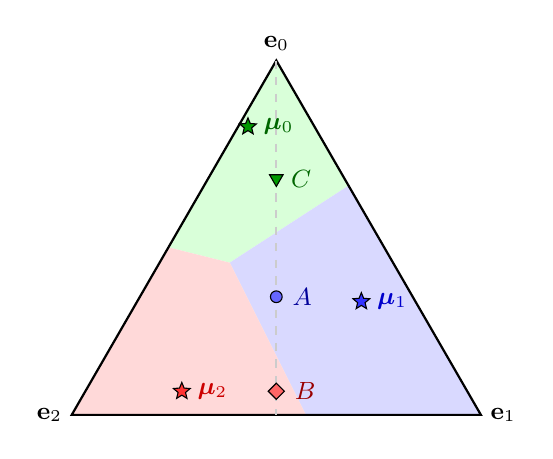
\begin{tikzpicture}[scale=0.6, font=\sffamily]

    % --- 1. Define Coordinates ---
    
    % The Triangle Vertices (Simplex)
    \coordinate (Top) at (0, 5);          
    \coordinate (Right) at (4.33, -2.5);  
    \coordinate (Left) at (-4.33, -2.5);  

    % The Prototypes (Stars)
    \coordinate (Mu0) at (-0.6, 3.6);    % Green (Top)
    \coordinate (Mu1) at (1.8, -0.1);    % Blue (Middle-Right)
    \coordinate (Mu2) at (-2.0, -2.0);   % Red (Bottom-Left)

    % The Data Points
    \coordinate (C) at (0, 2.5);   % Top Data
    \coordinate (A) at (0, 0);     % Middle Data
    \coordinate (B) at (0, -2.0);  % Bottom Data

    % --- 2. Background Regions (Voronoi Clipping) ---
    % Note: We draw these first so they are behind everything else
    
    % Region 0 (Green)
    \begin{scope}
        \clip (Top) -- (Right) -- (Left) -- cycle; 
        \path (Mu0) -- (Mu1) coordinate[midway] (M01);
        \clip ($(M01)!20cm!90:(Mu1)$) -- ($(M01)!20cm!-90:(Mu1)$) -- ($(M01)!20cm!180:(Mu1)$) -- cycle;
        \path (Mu0) -- (Mu2) coordinate[midway] (M02);
        \clip ($(M02)!20cm!90:(Mu2)$) -- ($(M02)!20cm!-90:(Mu2)$) -- ($(M02)!20cm!180:(Mu2)$) -- cycle;
        \fill[green!15] (-5,-5) rectangle (5,5);
    \end{scope}

    % Region 1 (Blue)
    \begin{scope}
        \clip (Top) -- (Right) -- (Left) -- cycle;
        \path (Mu1) -- (Mu0) coordinate[midway] (M10);
        \clip ($(M10)!20cm!90:(Mu0)$) -- ($(M10)!20cm!-90:(Mu0)$) -- ($(M10)!20cm!180:(Mu0)$) -- cycle;
        \path (Mu1) -- (Mu2) coordinate[midway] (M12);
        \clip ($(M12)!20cm!90:(Mu2)$) -- ($(M12)!20cm!-90:(Mu2)$) -- ($(M12)!20cm!180:(Mu2)$) -- cycle;
        \fill[blue!15] (-5,-5) rectangle (5,5);
    \end{scope}

    % Region 2 (Red)
    \begin{scope}
        \clip (Top) -- (Right) -- (Left) -- cycle;
        \path (Mu2) -- (Mu0) coordinate[midway] (M20);
        \clip ($(M20)!20cm!90:(Mu0)$) -- ($(M20)!20cm!-90:(Mu0)$) -- ($(M20)!20cm!180:(Mu0)$) -- cycle;
        \path (Mu2) -- (Mu1) coordinate[midway] (M21);
        \clip ($(M21)!20cm!90:(Mu1)$) -- ($(M21)!20cm!-90:(Mu1)$) -- ($(M21)!20cm!180:(Mu1)$) -- cycle;
        \fill[red!15] (-5,-5) rectangle (5,5);
    \end{scope}

    % --- 3. Draw Boundaries (Bisector Lines) ---
    % \begin{scope}
    %     \clip (Top) -- (Right) -- (Left) -- cycle;
    %     \draw[thick, green!50!black] ($(M01)!10cm!90:(Mu1)$) -- ($(M01)!10cm!-90:(Mu1)$);
    %     \draw[thick, blue!50!black] ($(M12)!10cm!90:(Mu2)$) -- ($(M12)!10cm!-90:(Mu2)$);
    %     \draw[thick, red!50!black] ($(M02)!10cm!90:(Mu2)$) -- ($(M02)!10cm!-90:(Mu2)$);
    % \end{scope}

    % --- 4. Main Triangle Frame & Blind Spot Line ---
    \draw[thick] (Top) -- (Right) -- (Left) -- cycle;
    \draw[dashed, gray!40, thick] (0, 5) -- (0, -2.5);

    % --- 5. Labels ---
    \node[above, font=\small] at (Top) {$\mathbf{e}_0$};
    \node[right, font=\small] at (Right) {$\mathbf{e}_1$};
    \node[left, font=\small] at (Left) {$\mathbf{e}_2$};

    % --- 6. Prototypes (Stars) ---
    \node[star, star points=5, star point ratio=2.25, fill=green!60!black, draw=black, inner sep=1pt] (Star0) at (Mu0) {};
    \node[right, green!40!black, font=\small\bfseries] at (Star0.east) {$\boldsymbol{\mu}_0$};
    
    \node[star, star points=5, star point ratio=2.25, fill=blue!80, draw=black, inner sep=1pt] (Star1) at (Mu1) {};
    \node[right, blue!80!black, font=\small\bfseries] at (Star1.east) {$\boldsymbol{\mu}_1$};
    
    \node[star, star points=5, star point ratio=2.25, fill=red!80, draw=black, inner sep=1pt] (Star2) at (Mu2) {};
    \node[right, red!80!black, font=\small\bfseries] at (Star2.east) {$\boldsymbol{\mu}_2$};

    % --- 7. Data Points ---
    % C (True: 0)
    \node[regular polygon, regular polygon sides=3, rotate=180, fill=green!60!black, draw=black, inner sep=1pt] (NodeC) at (C) {};
    \node[right, green!40!black, font=\small\bfseries] at (NodeC.west) {$C$};

    % A (True: 1)
    \node[circle, fill=blue!60, draw=black, inner sep=1.5pt] (NodeA) at (A) {};
    \node[right, blue!60!black, font=\small\bfseries] at (NodeA.east) {$A$};

    % B (True: 2)
    \node[diamond, fill=red!60, draw=black, inner sep=1.5pt] (NodeB) at (B) {};
    \node[right, red!60!black, font=\small\bfseries] at (NodeB.east) {$B$};

    % % --- 8. Legend ---
    % \matrix [draw, fill=white, fill opacity=0.9, anchor=south east, nodes={scale=0.8, anchor=west}] at (Right) {
    %     \node [regular polygon, regular polygon sides=3, rotate=180, fill=green!60!black, inner sep=1.5pt, label=right:Class 0] {}; \\
    %     \node [circle, fill=blue!60, inner sep=2pt, label=right:Class 1] {}; \\
    %     \node [diamond, fill=red!60, inner sep=2.5pt, label=right:Class 2] {}; \\
    %     \node [star, star points=5, fill=black, inner sep=2pt, label=right:Prototypes] {}; \\
    % };

\end{tikzpicture}
\end{document}
        \caption{Voronoi resolution of the vertical-stack configuration. Points $C, A, B$ lie along the altitude $p_1 = p_2$ that is invariant under the parallel-shift class-1-vs-2 score (Eq.~\ref{eq:vertical_stack_invariance}). Voronoi prototypes placed at distinct altitudes recover the correct partition into three horizontal strata.}\label{fig:voronoi_proof}
    \end{figure}

    Under $0/1$ loss, $\mathbf{c}_1 - \mathbf{c}_2 = (0, -1, 1)^\top$, so the difference between class-$1$ and class-$2$ parallel-shift scores is
    \begin{equation}\label{eq:vertical_stack_invariance}
        s_1(\mathbf{p}) - s_2(\mathbf{p}) = (\alpha_1 - \alpha_2) + (p_2 - p_1).
    \end{equation}
    Whenever $p_1 = p_2$ the cost terms of classes $1$ and $2$ coincide, so classifying $\mathbf{p}_A$ as $1$ forces $s_1(\mathbf{p}_A) \le s_2(\mathbf{p}_A)$, i.e.\ $\alpha_1 \le \alpha_2$, and classifying $\mathbf{p}_B$ as $2$ forces $\alpha_2 \le \alpha_1$. Both hold only if $\alpha_1 = \alpha_2$, whereupon $s_1 \equiv s_2$ on the altitude and $\mathbf{p}_A, \mathbf{p}_B$ receive the same label, so at least one of them is misclassified. Every parallel-shift rule therefore errs on at least one of the three points, giving $\inf_{\delta \in \mathcal{H}_{PS}} R(\delta) \ge 1/3 > 0$.

    Take $\boldsymbol{\mu}_0 = \mathbf{e}_0$, $\boldsymbol{\mu}_1 = (0.4, 0.5, 0.1)^\top$, $\boldsymbol{\mu}_2 = (0.1, 0.4, 0.5)^\top$. Direct computation shows~\eqref{eq:thm_vertex_consistency} holds for every $k$ (e.g., for $k = 1$, $\|\mathbf{e}_1 - \boldsymbol{\mu}_1\|_2^2 = 0.42 < 0.62 = \|\mathbf{e}_1 - \boldsymbol{\mu}_2\|_2^2 < 2 = \|\mathbf{e}_1 - \boldsymbol{\mu}_0\|_2^2$), so $\mathcal{M} \in \mathcal{H}_{Vor}^{\mathrm{DLC}}$. The squared distances at the two ambiguous points are
    \[
        d^2(\mathbf{p}_A, \boldsymbol{\mu}_1) = 0.08 < 0.14 = d^2(\mathbf{p}_A, \boldsymbol{\mu}_2), \qquad
        d^2(\mathbf{p}_B, \boldsymbol{\mu}_2) = 0.02 < 0.32 = d^2(\mathbf{p}_B, \boldsymbol{\mu}_1),
    \]
    so $\mathbf{p}_A \in \mathcal{P}_1^{\mathcal{M}}$ and $\mathbf{p}_B \in \mathcal{P}_2^{\mathcal{M}}$. At the third point $d^2(\mathbf{p}_C, \boldsymbol{\mu}_0) = 0.06 < 0.32 = d^2(\mathbf{p}_C, \boldsymbol{\mu}_1)$ and $< 0.74 = d^2(\mathbf{p}_C, \boldsymbol{\mu}_2)$, so $\mathbf{p}_C \in \mathcal{P}_0^{\mathcal{M}}$. All three points are thus classified to their true labels, so $R = 0$; since $\inf_{\delta \in \mathcal{H}_{PS}} R(\delta) \ge 1/3$, the strict separation $\inf_{\delta \in \mathcal{H}_{Vor}^{\mathrm{DLC}}} R(\delta) < \inf_{\delta \in \mathcal{H}_{PS}} R(\delta)$ follows. The Voronoi rule achieves this by placing prototypes at distinct altitudes, exploiting the $p_0$ direction that the parallel-shift score~\eqref{eq:vertical_stack_invariance} cannot see.
\end{proof}
\par
%!TeX root=../carlo_master.tex
\chapter{K-invariance of the misspecification budget}\label{app:kl_invariance}

The sweep parameters of Sections~\ref{sec:misspec_sensitivity_variance} and~\ref{sec:misspec_sensitivity_meanshift} are stated to be ``K-independent'', meaning that the per-$K$ curves can be overlaid on a common horizontal axis without an extra rescaling. The strongest sense in which this holds is that the KL divergence between the reference and perturbed distributions depends only on the sweep parameter and not on the number of classes. This appendix records the elementary computation for each construction.

\section{Variance scaling}

For the variance-scaling family of Section~\ref{sec:misspec_sensitivity_variance}, both members share uniform priors $\pi_k = 1/K$ and isotropic Gaussian class-conditionals on $\mathbb{R}^d$ with $d = 2$: the reference is $p_1(\cdot \mid Y{=}k) = \mathcal{N}(\mathbf{m}_k, \sigma^2 \mathbf{I})$ and the perturbed member is $p_\lambda(\cdot \mid Y{=}k) = \mathcal{N}(\mathbf{m}_k, \lambda\sigma^2 \mathbf{I})$. The general multivariate-Gaussian formula reads
\begin{equation}\label{eq:kl_gaussian_general}
    D_{\mathrm{KL}}\bigl(\mathcal{N}(\boldsymbol{\mu}_0, \Sigma_0) \,\big\|\, \mathcal{N}(\boldsymbol{\mu}_1, \Sigma_1)\bigr) = \tfrac{1}{2}\Bigl[\mathrm{tr}(\Sigma_1^{-1}\Sigma_0) - d + \log\tfrac{\det \Sigma_1}{\det \Sigma_0} + (\boldsymbol{\mu}_1 - \boldsymbol{\mu}_0)^\top \Sigma_1^{-1}(\boldsymbol{\mu}_1 - \boldsymbol{\mu}_0)\Bigr].
\end{equation}
Specialising to $\boldsymbol{\mu}_0 = \boldsymbol{\mu}_1 = \mathbf{m}_k$, $\Sigma_0 = \sigma^2 \mathbf{I}$, and $\Sigma_1 = \lambda\sigma^2 \mathbf{I}$ collapses the four terms in order: $\mathrm{tr}((\lambda\sigma^2)^{-1}\sigma^2 \mathbf{I}) = d/\lambda$, the dimension contributes $-d$, the log-determinant ratio is $\log(\lambda\sigma^2/\sigma^2)^d = d\log\lambda$, and the quadratic mean-difference term vanishes. Combining the three surviving terms gives
\begin{equation}\label{eq:kl_variance_perclass}
    D_{\mathrm{KL}}\bigl(p_1(\cdot \mid Y{=}k) \,\big\|\, p_\lambda(\cdot \mid Y{=}k)\bigr) = \tfrac{1}{2}\bigl(d/\lambda - d + d\log\lambda\bigr) = \frac{d}{2}\left(\log \lambda + \frac{1}{\lambda} - 1\right).
\end{equation}
The right-hand side depends on $\lambda$ and on the ambient dimension $d = 2$, but not on $K$. By the chain rule of relative entropy, $D_{\mathrm{KL}}(\mathbb{P}_1 \,\|\, \mathbb{P}_\lambda)$ equals the KL between the $Y$-marginals plus the $\pi$-weighted average of the per-class KLs on $X \mid Y$; the marginal term vanishes because the two distributions share the uniform $Y$-marginal, and the per-class summand is constant in $k$, so
\begin{equation}\label{eq:kl_variance_joint}
    D_{\mathrm{KL}}(\mathbb{P}_1 \,\|\, \mathbb{P}_\lambda) = \sum_{k=0}^{K-1} \pi_k\, D_{\mathrm{KL}}\bigl(p_1(\cdot \mid Y{=}k) \,\big\|\, p_\lambda(\cdot \mid Y{=}k)\bigr) = \frac{d}{2}\left(\log \lambda + \frac{1}{\lambda} - 1\right).
\end{equation}
Fixing $\lambda$ therefore fixes the per-class and joint KL budgets at the same value for every $K$, so the per-$K$ curves of Figure~\ref{fig:misspec-sensitivity-variance} are comparable along the horizontal axis without renormalisation.

\section{Random per-class mean shifts}

The mean-shift family of Section~\ref{sec:misspec_sensitivity_meanshift} replaces each class mean $\mathbf{m}_k$ by $\mathbf{m}_k + \xi\,\mathbf{v}_k$ in $\mathbb{R}^{K-1}$, with the per-class covariance fixed at $\sigma^2 \mathbf{I}$. The ambient dimension now scales with $K$, but specialising Eq.~\eqref{eq:kl_gaussian_general} to $\Sigma_0 = \Sigma_1 = \sigma^2 \mathbf{I}$ kills the trace and log-determinant contributions ($\mathrm{tr}((\sigma^2)^{-1}\sigma^2 \mathbf{I}) - d = 0$, $\log(\det \sigma^2 \mathbf{I}/\det \sigma^2 \mathbf{I}) = 0$) and leaves only the quadratic mean-difference term, so the per-class KL reduces to the squared Euclidean distance between the means relative to $\sigma^2$:
\begin{equation}\label{eq:kl_meanshift_perclass}
    D_{\mathrm{KL}}\bigl(p_0(\cdot \mid Y{=}k) \,\big\|\, p_\xi(\cdot \mid Y{=}k)\bigr) = \frac{(\xi\,\mathbf{v}_k)^\top (\sigma^2 \mathbf{I})^{-1} (\xi\,\mathbf{v}_k)}{2} = \frac{\|\xi\,\mathbf{v}_k\|^2}{2\sigma^2} = \frac{\xi^2}{2\sigma^2},
\end{equation}
using $\|\mathbf{v}_k\| = 1$ in the last step. The right-hand side depends on $\xi/\sigma$ alone and is constant in $k$, so the same chain-rule argument as in Eq.~\eqref{eq:kl_variance_joint} (shared uniform $Y$-marginal, per-class summand independent of $k$) gives a joint KL of $\xi^2/(2\sigma^2)$. The horizontal axis $\xi/\sigma$ of Figure~\ref{fig:misspec-sensitivity-meanshift} is therefore a K-independent misspecification budget, exactly as $\lambda$ is in the variance case.

The same calculation applied to the reference family $\mathbb{P}_0$ alone explains the $R_{\mathrm{circ}}(K) = 2\sigma\sqrt{2(K-1)/K}$ rescaling of Section~\ref{sec:misspec_sensitivity_meanshift}: for any pair $j \neq k$ of equal-covariance class-conditional Gaussians of $\mathbb{P}_0$ the same specialisation of Eq.~\eqref{eq:kl_gaussian_general} gives $D_{\mathrm{KL}}(p_0(\cdot \mid Y{=}j) \,\|\, p_0(\cdot \mid Y{=}k)) = \|\mathbf{m}_j - \mathbf{m}_k\|^2/(2\sigma^2)$. The choice of $R_{\mathrm{circ}}(K)$ that pins the pairwise Euclidean distance at $4\sigma$ for every $K$ therefore pins the pairwise KL at $(4\sigma)^2/(2\sigma^2) = 8$. The reference geometry and the perturbation are then both calibrated to K-independent KL budgets; what still varies with $K$ is the number of classes, and with it the ambient dimension $K-1$ of the simplex.
\par
%!TeX root=../carlo_master.tex
\chapter{Complexity measures for hypothesis classes}\label{app:complexity}

Three capacity measures control the uniform convergence arguments in this dissertation, each matched to a different output type. All yield bounds of the form
\begin{equation}
    R \leq \hat{R} + c\, \sqrt{\frac{d}{m}},
\end{equation}
where $d$ is the relevant capacity measure and $c$ is a factor that depends on $m$, $K$, and $1/\nu$ through logarithms, multiplied by $C_{max}$ when the loss is bounded by $C_{max}$. For the decision classes the factor is explicit, $c_{bin}$ in Eq.~\eqref{eq:clean_gen_bound} and $c_{Nat}$ in Remark~\ref{rem:natarajan_gen_bound}, under the hypotheses stated there. Because the rate has the same form, calibration complexity and decision complexity can be compared on equal footing. These are worst-case uniform-convergence rates: a small $d$ makes the bound tight only once $m \geq c^2 d/\epsilon^2$, so the realized benefit of a low-capacity decision layer is governed by the available validation label budget, not by $d$ alone.

The three measures also nest into one another:
\begin{itemize}
    \item $d_P$ reduces to $d_{VC}$ when functions are binary-valued.
    \item $d_{Nat}$ reduces to $d_{VC}$ when $K = 2$.
    \item For multiclass classifiers induced by real-valued scores
          ($\delta(\mathbf{p}) = \mathrm{argmin}_{k \in \mathcal{Y}}\, s_k(\mathbf{p})$),
          the Natarajan dimension of a $W$-parameter linear-score class is at most $W$
          (Lemma~\ref{lem:linear_embedding}).
\end{itemize}

Table~\ref{tab:complexity_unified} maps each pipeline component to its complexity measure.

\begin{table}[H]
    \centering\small
    \begin{tabular}{@{}llll@{}}
        \toprule
        \textbf{Component} & \textbf{Output} & \textbf{Measure} & \textbf{Where Used} \\
        \midrule
        Binary threshold $\delta_\tau$ & $\{0,1\}$ & $d_{VC}$
            & Lemma~\ref{lem:vc_thresh}, Prop.~\ref{prop:gen_bound} \\
        Multiclass decision $\delta\colon \Delta^{K-1}\!\to\!\mathcal{Y}$ & $\{0,\ldots,K{-}1\}$ & $d_{Nat}$
            & Secs.~\ref{sec:partition_optimization},~\ref{sec:voronoi_tessellation} \\
        Binary calibrator $g\colon [0,1]\!\to\![0,1]$ & $\mathbb{R}$ & $d_P$
            & Prop.~\ref{prop:calibrator_complexity} \\
        Multiclass calibrator $g\colon \Delta^{K-1}\!\to\!\Delta^{K-1}$ & $\mathbb{R}^K$ & $d_P$ (per class)
            & Sec.~\ref{sec:multiclass_calibration} \\
        \bottomrule
    \end{tabular}
    \caption{Mapping from pipeline components to complexity measures.}\label{tab:complexity_unified}
\end{table}

The decision classes of Chapters~\ref{sec:partition_optimization} and~\ref{sec:voronoi_tessellation} ($\mathcal{H}_{Full}$, $\mathcal{H}_{PS}$, $\mathcal{H}_{Vor}$, $\mathcal{H}_{Vor}^{\Delta}$) are all multiclass rules of the form $\mathbf{p} \mapsto \mathrm{argmin}_{k \in \mathcal{Y}} s_k(\mathbf{p}; w)$ whose per-class scores $s_k$ are controlled by a finite parameter $w$. We give a single embedding argument that bounds the Natarajan dimension (Definition~\ref{def:natarajan_dimension}) of all four, and identify which of the chapter bounds are exact and which hold only up to the constant absorbed by the embedding.

The argument uses the following external result. Fix per-class feature maps $\Phi_k: \Delta^{K-1} \to \mathbb{R}^{W}$ and let $\mathcal{H}_\Phi = \{\, \mathbf{p} \mapsto \mathrm{argmax}_{k \in \mathcal{Y}}\, w^\top \Phi_k(\mathbf{p}) : w \in \mathbb{R}^{W} \,\}$ be the free linear-score class they induce, with $w$ ranging over all of $\mathbb{R}^{W}$. The bound established by \citet[Theorem~7]{danielyshalev2014optimal}, $d_{Nat}(\mathcal{H}_\Phi) \leq W$, is the multiclass counterpart of the $W$-parameter VC bound for binary linear classifiers; negating $w$ exchanges $\mathrm{argmax}$ and $\mathrm{argmin}$ and leaves the bound unchanged.

\begin{lemma}[Subclass monotonicity]\label{lem:nat_monotone}
    If $\mathcal{H}' \subseteq \mathcal{H}$ then $d_{Nat}(\mathcal{H}') \leq d_{Nat}(\mathcal{H})$.
\end{lemma}
\begin{proof}
    A set N-shattered by $\mathcal{H}'$ with target functions $f_0, f_1$ is N-shattered by $\mathcal{H}$ with the same $f_0, f_1$, since every hypothesis the shattering requires belongs to $\mathcal{H}' \subseteq \mathcal{H}$. The largest N-shattered cardinality therefore cannot decrease when the class is enlarged.
\end{proof}

\begin{lemma}[Linear-score embedding]\label{lem:linear_embedding}
    Let $\mathcal{H} = \{\, \mathbf{p} \mapsto \mathrm{argmin}_{k \in \mathcal{Y}} s_k(\mathbf{p}; w) : w \in \mathbb{R}^{W} \,\}$ with
    \begin{equation}
        s_k(\mathbf{p}; w) = w^\top \Phi_k(\mathbf{p}) + g_k(\mathbf{p}),
    \end{equation}
    where $\Phi_k: \Delta^{K-1} \to \mathbb{R}^{W}$ and $g_k: \Delta^{K-1} \to \mathbb{R}$ are fixed and independent of $w$. Then $d_{Nat}(\mathcal{H}) \leq W$. If instead the per-class scores are affine in a lifted parameter of dimension $\widetilde{W}$, into which the structural parameters of $\mathcal{H}$ map by a fixed (possibly nonlinear) rule, then $\mathcal{H}$ is a subclass of the corresponding free linear-score class and $d_{Nat}(\mathcal{H}) \leq \widetilde{W}$.
\end{lemma}
\begin{proof}
    Let $C = \{\mathbf{p}_1, \ldots, \mathbf{p}_m\} \subseteq \Delta^{K-1}$ be N-shattered by $\mathcal{H}$ (Definition~\ref{def:natarajan_dimension}) with witness functions $f_0, f_1: C \to \mathcal{Y}$, $f_0(\mathbf{p}) \neq f_1(\mathbf{p})$ for all $\mathbf{p} \in C$. For each $\mathbf{p} \in C$ define the difference vector and the fixed scalar offset
    \begin{equation*}
        \boldsymbol{\rho}(\mathbf{p}) = \Phi_{f_0(\mathbf{p})}(\mathbf{p}) - \Phi_{f_1(\mathbf{p})}(\mathbf{p}) \in \mathbb{R}^{W}, \qquad
        h(\mathbf{p}) = g_{f_0(\mathbf{p})}(\mathbf{p}) - g_{f_1(\mathbf{p})}(\mathbf{p}) \in \mathbb{R},
    \end{equation*}
    where $h(\mathbf{p})$ does not depend on $w$. Then $s_{f_0(\mathbf{p})}(\mathbf{p}; w) - s_{f_1(\mathbf{p})}(\mathbf{p}; w) = w^\top \boldsymbol{\rho}(\mathbf{p}) + h(\mathbf{p})$. Suppose $m > W$. The $m$ difference vectors $\boldsymbol{\rho}(\mathbf{p})$ are then linearly dependent, so there are coefficients $c_{\mathbf{p}}$, not all zero, with $\sum_{\mathbf{p} \in C} c_{\mathbf{p}} \boldsymbol{\rho}(\mathbf{p}) = \mathbf{0}$. For every parameter $w$ the weighted sum of score gaps is therefore the same number,
    \begin{equation*}
        \sum_{\mathbf{p} \in C} c_{\mathbf{p}} \bigl(s_{f_0(\mathbf{p})}(\mathbf{p}; w) - s_{f_1(\mathbf{p})}(\mathbf{p}; w)\bigr) = \sum_{\mathbf{p} \in C} c_{\mathbf{p}}\, h(\mathbf{p}).
    \end{equation*}
    By N-shattering, some $w$ realizes the labeling that selects $f_0(\mathbf{p})$ where $c_{\mathbf{p}} > 0$ and $f_1(\mathbf{p})$ where $c_{\mathbf{p}} < 0$. Since the rule is an $\mathrm{argmin}$, the selected label has the smaller or equal score, so every summand on the left is nonpositive. Some other $w$ realizes the opposite labeling, for which every summand is nonnegative. Both sums equal the same fixed number, which is therefore zero, so every summand with $c_{\mathbf{p}} \neq 0$ vanishes in both realizations: at such a point $f_0(\mathbf{p})$ and $f_1(\mathbf{p})$ tie as minimizers in both realizations, yet opposite labels are selected. This is impossible under the smallest-index tie-breaking rule: when both labels minimize the score, the rule can select only the smaller of them. Hence $|C| = m \le W$, and $d_{Nat}(\mathcal{H}) \le W$. With $g_k \equiv 0$ this is exactly the bound of \citet[Theorem~7]{danielyshalev2014optimal} for the free class $\mathcal{H}_\Phi$. In the lifted case, the structural parameters of $\mathcal{H}$ map by a fixed (possibly nonlinear) rule into the free linear-score class of dimension $\widetilde{W}$, so $\mathcal{H}$ is a subclass of it and Lemma~\ref{lem:nat_monotone} with \citet[Theorem~7]{danielyshalev2014optimal} gives $d_{Nat}(\mathcal{H}) \leq \widetilde{W}$.
\end{proof}

Table~\ref{tab:partition_natarajan} instantiates the two lemmas for the four classes. For $\mathcal{H}_{PS}$ the scores are affine in the learnable parameter and the bound is exact: the $\leq K-1$ upper bound matches the explicit shattering of $K-1$ points in the proof of Theorem~\ref{thm:ps_complexity}, giving $d_{Nat}(\mathcal{H}_{PS}) = K-1$. For $\mathcal{H}_{Full}$ the same embedding gives the upper bound $\leq K^2$; the inclusion $\mathcal{H}_{PS} \subseteq \mathcal{H}_{Full}$ supplies only the lower bound $\geq K-1$, so $d_{Nat}(\mathcal{H}_{Full})$ is bounded as $\leq K^2$ without a matching quadratic lower bound. For the Voronoi classes the squared-norm bias couples the weight and offset of each prototype, so the embedding is the coupled case: the prototype coordinates ($K^2$ for $\mathcal{H}_{Vor}$, $K(K-1)$ for $\mathcal{H}_{Vor}^{\Delta}$) are the free parameters, the lifted free class adds one offset per class, and Lemma~\ref{lem:linear_embedding} yields the bounds $\leq K^2+K$ and $\leq K^2$ respectively.

\begin{table}[h]
    \centering
    \begin{tabular}{@{}lllll@{}}
        \toprule
        Class & Free parameters & Fixed term $g_k$ & Lemma~\ref{lem:linear_embedding} & $d_{Nat}$ \\
        \midrule
        $\mathcal{H}_{Full}$ & $K^2$ ($\mathbf{A}$) & none & $\leq K^2$ & $\leq K^2$ \\
        $\mathcal{H}_{PS}$ & $K-1$ ($\mathbf{v}$) & $\mathbf{c}_k^\top \mathbf{p}$ & $\leq K-1$ & $= K-1$ \\
        $\mathcal{H}_{Sc}$ & $K-1$ ($\boldsymbol{\beta}$, gauge $\beta_0{=}1$) & $C_{0k}\,p_0$ & $\leq K-1$ & $\leq K-1$ \\
        $\mathcal{H}_{Vor}$ & $K^2$ (prototypes, coupled) & none & $\leq K^2 + K$ & $\leq K^2$ \\
        $\mathcal{H}_{Vor}^{\Delta}$ & $K(K-1)$ (prototypes, coupled) & none & $\leq K^2$ & $\leq K^2$ \\
        \bottomrule
    \end{tabular}
    \caption{Natarajan-dimension bounds for the partition score classes via Lemmas~\ref{lem:nat_monotone} and~\ref{lem:linear_embedding}. Lower bounds: the explicit shattering of $K-1$ points in the proof of Theorem~\ref{thm:ps_complexity} gives the matching bound $d_{Nat}(\mathcal{H}_{PS}) = K-1$; propagated through the inclusions $\mathcal{H}_{PS} \subseteq \mathcal{H}_{Full}$ and $\mathcal{H}_{PS} \subseteq \mathcal{H}_{Vor}$ (Proposition~\ref{prop:ps_in_vor}) it yields only the lower bound $\geq K-1$ for the remaining classes, whose dimensions are therefore reported as the stated upper bounds rather than matching quadratic orders.}\label{tab:partition_natarajan}
\end{table}

\begin{remark}\label{rem:voronoi_embedding_bounds}
    The embedding bounds for $\mathcal{H}_{Vor}$ and $\mathcal{H}_{Vor}^{\Delta}$ are the prototype counts plus a per-class bias. The lifted linear-score class adds one bias coordinate per class, so the embedding gives $\leq K^2 + K$ and $\leq K^2$ respectively; for $\mathcal{H}_{Vor}$, Theorem~\ref{thm:voronoi_complexity} improves the first to the $\leq K^2$ bound for $\mathcal{H}_{Full}$. The value of the Voronoi parameterization is therefore the prototype geometry, the DLC, and the sampler that preserves it, not a lower capacity bound.
\end{remark}
\par
%!TeX root=../carlo_master.tex
\chapter{Computational resources}\label{app:compute}

The empirical campaigns of Sections~\ref{sec:binary_experiments} and~\ref{sec:multiclass_experiments} ran on rented cloud virtual machines; the synthetic studies of Section~\ref{sec:voronoi_comparison}, the boundary-rotation scenario of Section~\ref{sec:boundary_rotation_experiment}, and all table and figure generation ran locally on a personal laptop. Cloud machine-type selection, bootstrap, and run discipline are documented in \texttt{experiments/cloud/README.md}.

\paragraph{Cloud hardware.} Two virtual-machine types covered the OpenML benchmarks, running in parallel and merging their per-seed parquet shards on the laptop after each campaign. A Google Cloud CPU instance (\texttt{n2-highcpu-80}: 80 Intel Ice~Lake vCPUs, 80\,GB RAM, Ubuntu 24.04~LTS) ran the seven non-neural base estimators (GaussianNB, Logistic Regression, Random Forest, Extra Trees, XGBoost, LightGBM, CatBoost). A RunPod pod with one NVIDIA H200 (141\,GB HBM3e) on RunPod's CUDA~12.8 / PyTorch~2.8 PyTorch image ran the three deep tabular estimators (TabM, TabPFN, TabICLv2).

\paragraph{Per-study compute.} Each campaign uses ten replicate seeds and the dataset, model, strategy, and objective registries documented in its experimental-setup subsection. The merged parquets hold $136{,}680$ (dataset, model, objective, strategy, seed) rows for binary and $276{,}960$ for multiclass. Wall clock per leg, rounded: the CPU VM ran for ${\approx}\,10\,\text{min}$ on binary and ${\approx}\,2\,\text{h}$ on multiclass, and the H200 pod for ${\approx}\,2\,\text{h}$ on binary and ${\approx}\,25\,\text{min}$ on multiclass. The decision-stage \texttt{fit} calls themselves are a small fraction of total compute: the per-row \texttt{strategy\_fit\_seconds} field of the merged multiclass parquet sums to ${\approx}\,35\,\text{CPU-h}$ across all joblib workers, dominated by the five cross-validated tuning variants at ${\approx}\,5\text{--}6\,\text{CPU-h}$ each; on the binary side the harness caches base-model probabilities and replays them across objectives rather than refitting, keeping the recorded decision-stage cost negligible (${<}\,0.1\,\text{CPU-h}$).

\paragraph{Performance engineering.} The wall-clock figures above reflect a sequence of targeted optimizations to the harness and the \texttt{threshold\_opt} library; without them the multiclass campaign would have been several orders of magnitude more expensive. Three categories account for most of the gain. First, sharing cross-validation fold refits across the seven multiclass CV-variant strategies, which all use the same deterministic stratified $K$-fold split: refitting once per (dataset, model) and reusing through a pipeline-level cache dropped a representative smoke run from ${\approx}\,2.5\,\text{h}$ to under $30\,\text{min}$. Second, vectorizing the partition-optimizer inner loops and replacing finite-difference gradients in the Dirichlet calibrator with an analytical Jacobian, each yielding order-of-magnitude per-call speedups. Third, oversubscription control on the 80-vCPU CPU VM\@: base estimators are pinned to a single thread and the surrounding BLAS, OpenMP, and PyTorch pools are capped to one thread per joblib worker.

\paragraph{Total spend.} Total cloud spend over the project lifetime was approximately USD 140 on RunPod GPU and BRL 480 on Google Cloud CPU, inclusive of development-time smoke runs, GPU connection checks, and occasional resumed runs. The synthetic studies and the analysis pipeline added no cloud cost.

\paragraph{Reproducibility.} The merged parquets and per-row metadata (ten replicate seeds sampled deterministically from a master seed, the per-row \texttt{strategy\_fit\_seconds}, and the model-side test AUCs on both data partitions) are stored under \texttt{experiments/results/} and re-run end-to-end via \texttt{make experiments-binary} and \texttt{make experiments-multiclass}; the environment is pinned through a fixed \texttt{.python-version} and a committed \texttt{uv.lock}. A \texttt{pytest} suite over \texttt{src/} and \texttt{experiments/} (\texttt{make test}) covers the library and the harness, \texttt{make test-reproducibility} asserts that a fixed seed yields identical fits and predictions, and \texttt{make test-freshness} regenerates every committed table and figure from the stored results and fails on any diff against the versioned copy; the same suite runs in continuous integration on every push and pull request.
\par
%!TeX root=../carlo_master.tex
\chapter{Machine-checked proofs}\label{app:formalization}

The mathematical statements of this dissertation are also stated and proved in Lean~4 \citep{demoura2021lean4}, a proof assistant whose kernel accepts a proof only if every inference step is valid, using its mathematical library Mathlib \citep{mathlib2020}. The development is in the folder \texttt{lean/} of the accompanying repository. This appendix reports what it covers, how each formal statement is linked to the text, and what it does not establish. Verification concerns the stated mathematical results; it does not establish the correctness of the experimental software or of the empirical conclusions.

\section{Scope and method}\label{sec:formalization_method}

The development covers every theorem-like environment of the dissertation (definitions, assumptions, examples, lemmas, propositions, theorems, corollaries, and remarks) and nine displayed equations. It includes the decision-risk identities, conditional calibration, the simplex geometry of the decision regions, the capacity of the hypothesis classes, the generalization bounds, the Gaussian Kullback--Leibler computations, the moments of the uniform distribution on a sphere, and the invariant of the sequential sampler.

Each formal statement carries the \LaTeX{} label of the statement it represents as a Lean attribute. An audit program traverses the tagged declarations and records the axioms on which each proof depends. A script joins that record with the theorem-like environments of the dissertation source and generates the status table reproduced below. The audit rejects incomplete proofs and duplicate tags; the script rejects tags without a corresponding label and axioms outside the registered list. Whether a Lean statement says what its printed counterpart says is not checked by these programs; it rests on an AI-assisted comparison of each tagged statement with the text. The formal proof of a statement need not follow the printed argument.

\section{Proofs of cited results}\label{sec:formalization_axioms}

No result is assumed as an axiom. The uniform-convergence bound for classes of finite VC dimension \citep[Corollary~3.19]{mohri2018foundations}, which Proposition~\ref{prop:gen_bound} applies, is itself proved in the development through McDiarmid's inequality, symmetrization, Massart's lemma, and Sauer's lemma. The capacity results for pseudo-dimension and for multiclass linear-score classes are also proved. Every tagged proof depends only on the three standard axioms of Lean: propositional extensionality, the axiom of choice, and the soundness of quotients.

Hypotheses that the text states explicitly remain explicit in the formal statements: admissibility of the cost matrix, a common smoothness radius, and the approximation of a rule class by a countable class of measurable rules. The formal statements of the risk identities also assume that $\eta$ is the conditional law of the label given the input; such a conditional law exists for every data distribution in the formal setting.

\section{Status of each result}\label{sec:formalization_table}

A statement is \emph{Verified} when a Lean theorem proves it, or proves a stronger statement that implies it, with only the three standard axioms. A definition or assumption is \emph{Formalized} when it is transcribed and used by the development; it is not a proved result. Of the $40$ theorem-like environments, $30$ are verified statements and $10$ are formalized definitions or assumptions; none is verified only in part, and none lacks a Lean counterpart. Together with the nine displayed equations, there are $49$ tagged declarations and no incomplete proofs.

% Auto-generated by lean/scripts/render_table.py --- do not edit.
{\small
\renewcommand{\arraystretch}{1.15}
\begin{longtable}{@{}l >{\raggedright\arraybackslash}p{0.58\textwidth} l@{}}
\caption{Machine-checked status of every theorem-like statement in this dissertation.}\label{tab:formalization}\\
\toprule
\textbf{Statement} & \textbf{Lean declaration} & \textbf{Status} \\
\midrule
\endfirsthead

\multicolumn{3}{@{}l}{\textit{Table~\ref{tab:formalization} (continued)}}\\
\toprule
\textbf{Statement} & \textbf{Lean declaration} & \textbf{Status} \\
\midrule
\endhead

\bottomrule
\endlastfoot

\multicolumn{3}{@{}l}{\textit{Theoretical framework}}\\
\midrule
Proposition~\ref{prop:bayes_risk_identity} & \texttt{Risk.\allowbreak{}bayes\_risk\_identity} & Verified \\
Proposition~\ref{prop:excess_risk_bound} & \texttt{Risk.\allowbreak{}excess\_risk\_bound} & Verified \\
Definition~\ref{def:vc_dimension} & \texttt{Capacity.\allowbreak{}vcDim} & Formalized \\
Proposition~\ref{prop:gen_bound} & \texttt{SeparableBounds.\allowbreak{}gen\_bound\_binary\_thesis\_of\_approx} & Verified \\
Lemma~\ref{lem:vc_thresh} & \texttt{Capacity.\allowbreak{}vcDim\_thresholdClass} & Verified \\
\midrule
\multicolumn{3}{@{}l}{\textit{Binary classification ($K=2$)}}\\
\midrule
Lemma~\ref{lem:threshold_optimality} & \texttt{Binary.\allowbreak{}threshold\_optimality} & Verified \\
Definition~\ref{def:calibration} & \texttt{Binary.\allowbreak{}PerfectCalibration} & Formalized \\
Proposition~\ref{prop:calibrate_then_decide} & \texttt{Binary.\allowbreak{}calibrate\_then\_decide\_integrated} & Verified \\
Definition~\ref{def:pseudo_dimension} & \texttt{Capacity.\allowbreak{}pseudoDim} & Formalized \\
Proposition~\ref{prop:calibrator_complexity} & \texttt{Capacity.\allowbreak{}calibrator\_complexity} & Verified \\
\midrule
\multicolumn{3}{@{}l}{\textit{Multiclass classification ($K > 2$)}}\\
\midrule
Definition~\ref{def:admissibility} & \texttt{Multiclass.\allowbreak{}Admissible} & Formalized \\
Example~\ref{ex:inadmissible} & \texttt{Examples.\allowbreak{}not\_admissible\_inad} & Verified \\
Definition~\ref{def:elementwise} & \texttt{Multiclass.\allowbreak{}ElementwiseReasonable} & Formalized \\
Example~\ref{ex:hedge} & \texttt{Examples.\allowbreak{}elementwise\_strictly\_stronger} & Verified \\
Proposition~\ref{prop:elementwise_admissible} & \texttt{Examples.\allowbreak{}elementwise\_admissible} & Verified \\
Theorem~\ref{thm:rigid_partition} & \texttt{Multiclass.\allowbreak{}rigid\_partition} & Verified \\
\midrule
\multicolumn{3}{@{}l}{\textit{Approaches to partition optimization}}\\
\midrule
Proposition~\ref{prop:parallel_invariance} & \texttt{Partition.\allowbreak{}parallel\_invariance} & Verified \\
Proposition~\ref{prop:column_rotation} & \texttt{Partition.\allowbreak{}column\_rotation} & Verified \\
Proposition~\ref{prop:ratio_equivalence} & \texttt{Partition.\allowbreak{}ratio\_equivalence} & Verified \\
Proposition~\ref{prop:marchetti_equivalence} & \texttt{Partition.\allowbreak{}marchetti\_equivalence} & Verified \\
\midrule
\multicolumn{3}{@{}l}{\textit{Voronoi tessellations as decision hypothesis class}}\\
\midrule
Definition~\ref{def:voronoi_rule} & \texttt{Voronoi.\allowbreak{}voronoiRule} & Formalized \\
Proposition~\ref{prop:voronoi_full_equality} & \texttt{Complexity.\allowbreak{}HVor\_eq\_HFull} & Verified \\
Theorem~\ref{thm:rotational_dominance} & \texttt{Witness.\allowbreak{}rotational\_dominance} & Verified \\
Proposition~\ref{prop:ps_in_vor} & \texttt{Complexity.\allowbreak{}HPS\_ssubset\_HVor\_unrestricted} & Verified \\
Definition~\ref{def:dlc} & \texttt{Voronoi.\allowbreak{}DLC} & Formalized \\
Proposition~\ref{prop:seqd2_correct} & \texttt{SequentialSampler.\allowbreak{}seqd2\_correct} & Verified \\
Definition~\ref{def:natarajan_dimension} & \texttt{Capacity.\allowbreak{}natDim} & Formalized \\
Remark~\ref{rem:natarajan_gen_bound} & \texttt{PointwiseApprox.\allowbreak{}gen\_bound\_natarajan\_clean\_of\_approx\_event} & Verified \\
Theorem~\ref{thm:ps_complexity} & \texttt{Complexity.\allowbreak{}ps\_complexity} & Verified \\
Theorem~\ref{thm:sc_complexity} & \texttt{Complexity.\allowbreak{}sc\_complexity\_sharp} & Verified \\
Theorem~\ref{thm:full_complexity} & \texttt{Complexity.\allowbreak{}full\_complexity\_quadratic} & Verified \\
Theorem~\ref{thm:voronoi_complexity} & \texttt{Complexity.\allowbreak{}voronoi\_complexity\_quadratic} & Verified \\
Remark~\ref{rem:multiclass_calibration} & \texttt{Capacity.\allowbreak{}multiclass\_calibration} & Verified \\
\midrule
\multicolumn{3}{@{}l}{\textit{Sensitivity to estimation misspecification across K}}\\
\midrule
Assumption~\ref{ass:smoothness} & \texttt{Diffusion.\allowbreak{}LocalSmoothness} & Formalized \\
Assumption~\ref{ass:diffuse} & \texttt{Diffusion.\allowbreak{}Diffuse} & Formalized \\
Lemma~\ref{lem:dimensional_dilution} & \texttt{SphereSymmetry.\allowbreak{}dimensional\_dilution} & Verified \\
Corollary~\ref{cor:integrated_dilution} & \texttt{SphereSymmetry.\allowbreak{}integrated\_dilution} & Verified \\
\midrule
\multicolumn{3}{@{}l}{\textit{Complexity measures for hypothesis classes}}\\
\midrule
Lemma~\ref{lem:nat_monotone} & \texttt{Capacity.\allowbreak{}natDim\_mono} & Verified \\
Lemma~\ref{lem:linear_embedding} & \texttt{Capacity.\allowbreak{}natDim\_le\_of\_linear\_scores} & Verified \\
Remark~\ref{rem:voronoi_embedding_bounds} & \texttt{Complexity.\allowbreak{}voronoi\_complexity} & Verified \\
\midrule
\multicolumn{3}{@{}l}{\textit{Displayed equations}}\\
\midrule
Equation~\eqref{eq:clean_gen_bound} & \texttt{SeparableBounds.\allowbreak{}gen\_bound\_binary\_clean\_of\_approx} & Verified \\
Equation~\eqref{eq:dsq_identity} & \texttt{Voronoi.\allowbreak{}dsq\_vertex} & Verified \\
Equation~\eqref{eq:elkan_threshold} & \texttt{Binary.\allowbreak{}elkanThreshold\_mem\_Ioo} & Verified \\
Equation~\eqref{eq:kl_gaussian_general} & \texttt{GaussianKL.\allowbreak{}klDiv\_multivariateGaussian} & Verified \\
Equation~\eqref{eq:kl_meanshift_perclass} & \texttt{GaussianKL.\allowbreak{}kl\_meanshift\_perclass} & Verified \\
Equation~\eqref{eq:kl_variance_joint} & \texttt{GaussianKL.\allowbreak{}kl\_variance\_joint} & Verified \\
Equation~\eqref{eq:kl_variance_perclass} & \texttt{GaussianKL.\allowbreak{}kl\_variance\_perclass} & Verified \\
Equation~\eqref{eq:meanshift_pairwise} & \texttt{GaussianKL.\allowbreak{}pairwise\_dist} & Verified \\
Equation~\eqref{eq:seqd2_invariant} & \texttt{SequentialSampler.\allowbreak{}build\_invariant} & Verified \\
\end{longtable}
}


Table~\ref{tab:formalization} is generated from the checked declarations and the dissertation source.

\section{Reproducing the check}\label{sec:formalization_repro}

The development pins Lean~4.33.0 and the matching Mathlib release through the committed toolchain and manifest files. From the repository root, \texttt{make lean-setup} installs the toolchain manager and downloads the Mathlib build cache, \texttt{make lean-build} checks every proof, and \texttt{make lean-audit} regenerates the axiom record and Table~\ref{tab:formalization}. The table is committed, so compiling the dissertation does not require a Lean installation.
\par
%!TeX root=../carlo_master.tex
\chapter{How AI was used in this work}\label{app:ai-disclosure}

We are living through a period in which large language models have become a routine part of technical work. This dissertation studies decision strategies for classification, but the same probabilistic machinery that underpins the classifiers examined here also powers the writing and coding assistants that helped produce this document. This appendix gives an account of how they were used.

Assistants were used to draft and refactor the \texttt{threshold\_opt} library, the experiment harness and analysis scripts, the test suite, and the cloud tooling; to survey the related literature and inform the dataset selection toward diverse scenarios and overlap with data used by prior work; to locate candidate bibliographic references and page numbers, which were verified against the original sources; to draft and revise several prose subsections; and to generate and cross-check shorter derivations. Earlier in the project this was a web-based paste-in-and-out workflow; once the \LaTeX{} source was moved into the code repository it became an IDE-integrated loop in which a proposed diff was accepted, edited, or rejected before each commit, and during writing I ran one-shot ``cold reader'' passes asking a model to flag unsupported claims and inconsistencies between prose, tables, and figures. The analysis of the empirical results came out of the same loop: assistants proposed readings of the tables and figures, and the ones that appear here are those I judged correct.

The Lean formalization of Appendix~\ref{app:formalization} was generated by AI assistants, including the formal statements, their proofs, and the comparison of each tagged statement with the text. My own reading of the formal statements was limited by a basic knowledge of Lean; their agreement with the printed statements rests on the AI-assisted comparison. The Lean kernel guarantees that every formal theorem is proved. Working through the formalization also helped identify errors and missing hypotheses, which were then corrected.

The research questions and the theoretical contributions are mine.
\par

%%%%%%%%%%%%%%%%%%%%%%%%%%%%%%% BIBLIOGRAPHY %%%%%%%%%%%%%%%%%%%%%%%%%%%%%%%%%%%

\backmatter

\pagestyle{backmatter}

% Extra space in the ToC before the references.
\addtocontents{toc}{\vspace{2\baselineskip plus .5\baselineskip minus .5\baselineskip}}

\printbibliography[
  title=\refname\label{sec:bib},
  heading=bibintoc,
]

\end{document}
